\documentclass[twoside]{book}

% Packages required by doxygen
\usepackage{fixltx2e}
\usepackage{calc}
\usepackage{doxygen}
\usepackage[export]{adjustbox} % also loads graphicx
\usepackage{graphicx}
\usepackage[utf8]{inputenc}
\usepackage{makeidx}
\usepackage{multicol}
\usepackage{multirow}
\PassOptionsToPackage{warn}{textcomp}
\usepackage{textcomp}
\usepackage[nointegrals]{wasysym}
\usepackage[table]{xcolor}

% Font selection
\usepackage[T1]{fontenc}
\usepackage[scaled=.90]{helvet}
\usepackage{courier}
\usepackage{amssymb}
\usepackage{sectsty}
\renewcommand{\familydefault}{\sfdefault}
\allsectionsfont{%
  \fontseries{bc}\selectfont%
  \color{darkgray}%
}
\renewcommand{\DoxyLabelFont}{%
  \fontseries{bc}\selectfont%
  \color{darkgray}%
}
\newcommand{\+}{\discretionary{\mbox{\scriptsize$\hookleftarrow$}}{}{}}

% Page & text layout
\usepackage{geometry}
\geometry{%
  a4paper,%
  top=2.5cm,%
  bottom=2.5cm,%
  left=2.5cm,%
  right=2.5cm%
}
\tolerance=750
\hfuzz=15pt
\hbadness=750
\setlength{\emergencystretch}{15pt}
\setlength{\parindent}{0cm}
\setlength{\parskip}{3ex plus 2ex minus 2ex}
\makeatletter
\renewcommand{\paragraph}{%
  \@startsection{paragraph}{4}{0ex}{-1.0ex}{1.0ex}{%
    \normalfont\normalsize\bfseries\SS@parafont%
  }%
}
\renewcommand{\subparagraph}{%
  \@startsection{subparagraph}{5}{0ex}{-1.0ex}{1.0ex}{%
    \normalfont\normalsize\bfseries\SS@subparafont%
  }%
}
\makeatother

% Headers & footers
\usepackage{fancyhdr}
\pagestyle{fancyplain}
\fancyhead[LE]{\fancyplain{}{\bfseries\thepage}}
\fancyhead[CE]{\fancyplain{}{}}
\fancyhead[RE]{\fancyplain{}{\bfseries\leftmark}}
\fancyhead[LO]{\fancyplain{}{\bfseries\rightmark}}
\fancyhead[CO]{\fancyplain{}{}}
\fancyhead[RO]{\fancyplain{}{\bfseries\thepage}}
\fancyfoot[LE]{\fancyplain{}{}}
\fancyfoot[CE]{\fancyplain{}{}}
\fancyfoot[RE]{\fancyplain{}{\bfseries\scriptsize Generated by Doxygen }}
\fancyfoot[LO]{\fancyplain{}{\bfseries\scriptsize Generated by Doxygen }}
\fancyfoot[CO]{\fancyplain{}{}}
\fancyfoot[RO]{\fancyplain{}{}}
\renewcommand{\footrulewidth}{0.4pt}
\renewcommand{\chaptermark}[1]{%
  \markboth{#1}{}%
}
\renewcommand{\sectionmark}[1]{%
  \markright{\thesection\ #1}%
}

% Indices & bibliography
\usepackage{natbib}
\usepackage[titles]{tocloft}
\setcounter{tocdepth}{3}
\setcounter{secnumdepth}{5}
\makeindex

% Hyperlinks (required, but should be loaded last)
\usepackage{ifpdf}
\ifpdf
  \usepackage[pdftex,pagebackref=true]{hyperref}
\else
  \usepackage[ps2pdf,pagebackref=true]{hyperref}
\fi
\hypersetup{%
  colorlinks=true,%
  linkcolor=blue,%
  citecolor=blue,%
  unicode%
}

% Custom commands
\newcommand{\clearemptydoublepage}{%
  \newpage{\pagestyle{empty}\cleardoublepage}%
}

\usepackage{caption}
\captionsetup{labelsep=space,justification=centering,font={bf},singlelinecheck=off,skip=4pt,position=top}

%===== C O N T E N T S =====

\begin{document}

% Titlepage & ToC
\hypersetup{pageanchor=false,
             bookmarksnumbered=true,
             pdfencoding=unicode
            }
\pagenumbering{alph}
\begin{titlepage}
\vspace*{7cm}
\begin{center}%
{\Large Dragon\+Force\+Academy }\\
\vspace*{1cm}
{\large Generated by Doxygen 1.8.12}\\
\end{center}
\end{titlepage}
\clearemptydoublepage
\pagenumbering{roman}
\tableofcontents
\clearemptydoublepage
\pagenumbering{arabic}
\hypersetup{pageanchor=true}

%--- Begin generated contents ---
\chapter{Hierarchical Index}
\section{Class Hierarchy}
This inheritance list is sorted roughly, but not completely, alphabetically\+:\begin{DoxyCompactList}
\item \contentsline{section}{Binary\+Tree$<$ T $>$}{\pageref{class_binary_tree}}{}
\item \contentsline{section}{Binary\+Tree$<$ node\+Match $>$}{\pageref{class_binary_tree}}{}
\item \contentsline{section}{B\+T\+Itr\+In$<$ T $>$}{\pageref{class_b_t_itr_in}}{}
\item \contentsline{section}{B\+T\+Itr\+Level$<$ T $>$}{\pageref{class_b_t_itr_level}}{}
\item \contentsline{section}{B\+T\+Itr\+Post$<$ T $>$}{\pageref{class_b_t_itr_post}}{}
\item \contentsline{section}{B\+T\+Itr\+Pre$<$ T $>$}{\pageref{class_b_t_itr_pre}}{}
\item \contentsline{section}{B\+T\+Node$<$ T $>$}{\pageref{class_b_t_node}}{}
\item \contentsline{section}{B\+T\+Node$<$ node\+Match $>$}{\pageref{class_b_t_node}}{}
\item \contentsline{section}{Club}{\pageref{class_club}}{}
\item \contentsline{section}{Date}{\pageref{class_date}}{}
\item \contentsline{section}{E\+CG}{\pageref{class_e_c_g}}{}
\item \contentsline{section}{Fraction}{\pageref{class_fraction}}{}
\item \contentsline{section}{Info}{\pageref{class_info}}{}
\begin{DoxyCompactList}
\item \contentsline{section}{Info\+DF}{\pageref{class_info_d_f}}{}
\item \contentsline{section}{Info\+FW}{\pageref{class_info_f_w}}{}
\item \contentsline{section}{Info\+GK}{\pageref{class_info_g_k}}{}
\item \contentsline{section}{Info\+MF}{\pageref{class_info_m_f}}{}
\end{DoxyCompactList}
\item \contentsline{section}{Invalid\+Date}{\pageref{class_invalid_date}}{}
\item \contentsline{section}{Invalid\+Input}{\pageref{class_invalid_input}}{}
\item \contentsline{section}{Invalid\+Stream}{\pageref{class_invalid_stream}}{}
\item \contentsline{section}{Level}{\pageref{class_level}}{}
\item \contentsline{section}{Match}{\pageref{class_match}}{}
\item \contentsline{section}{Season}{\pageref{class_season}}{}
\item \contentsline{section}{Sort\+Training}{\pageref{class_sort_training}}{}
\item \contentsline{section}{Table}{\pageref{class_table}}{}
\item \contentsline{section}{Tournament}{\pageref{class_tournament}}{}
\item \contentsline{section}{Training}{\pageref{class_training}}{}
\item \contentsline{section}{Underflow}{\pageref{class_underflow}}{}
\item \contentsline{section}{Worker}{\pageref{class_worker}}{}
\begin{DoxyCompactList}
\item \contentsline{section}{Athlete}{\pageref{class_athlete}}{}
\begin{DoxyCompactList}
\item \contentsline{section}{Defender}{\pageref{class_defender}}{}
\item \contentsline{section}{Forward}{\pageref{class_forward}}{}
\item \contentsline{section}{Goalkeeper}{\pageref{class_goalkeeper}}{}
\item \contentsline{section}{Midfielder}{\pageref{class_midfielder}}{}
\end{DoxyCompactList}
\item \contentsline{section}{Coach}{\pageref{class_coach}}{}
\end{DoxyCompactList}
\end{DoxyCompactList}

\chapter{Class Index}
\section{Class List}
Here are the classes, structs, unions and interfaces with brief descriptions\+:\begin{DoxyCompactList}
\item\contentsline{section}{\hyperlink{class_athlete}{Athlete} \\*An athlete. }{\pageref{class_athlete}}{}
\item\contentsline{section}{\hyperlink{class_binary_tree}{Binary\+Tree$<$ T $>$} \\*A binary tree. }{\pageref{class_binary_tree}}{}
\item\contentsline{section}{\hyperlink{class_b_t_itr_in}{B\+T\+Itr\+In$<$ T $>$} \\*An in binary tree iterator. }{\pageref{class_b_t_itr_in}}{}
\item\contentsline{section}{\hyperlink{class_b_t_itr_level}{B\+T\+Itr\+Level$<$ T $>$} \\*A level binary tree iterator. }{\pageref{class_b_t_itr_level}}{}
\item\contentsline{section}{\hyperlink{class_b_t_itr_post}{B\+T\+Itr\+Post$<$ T $>$} \\*A post binary tree iterator. }{\pageref{class_b_t_itr_post}}{}
\item\contentsline{section}{\hyperlink{class_b_t_itr_pre}{B\+T\+Itr\+Pre$<$ T $>$} \\*A pre binary tree iterator. }{\pageref{class_b_t_itr_pre}}{}
\item\contentsline{section}{\hyperlink{class_b_t_node}{B\+T\+Node$<$ T $>$} \\*A binary tree node. }{\pageref{class_b_t_node}}{}
\item\contentsline{section}{\hyperlink{class_club}{Club} \\*A club. }{\pageref{class_club}}{}
\item\contentsline{section}{\hyperlink{class_coach}{Coach} \\*A coach. }{\pageref{class_coach}}{}
\item\contentsline{section}{\hyperlink{class_date}{Date} }{\pageref{class_date}}{}
\item\contentsline{section}{\hyperlink{class_defender}{Defender} \\*A defender. }{\pageref{class_defender}}{}
\item\contentsline{section}{\hyperlink{class_e_c_g}{E\+CG} \\*An ecg. }{\pageref{class_e_c_g}}{}
\item\contentsline{section}{\hyperlink{class_forward}{Forward} \\*A forward. }{\pageref{class_forward}}{}
\item\contentsline{section}{\hyperlink{class_fraction}{Fraction} }{\pageref{class_fraction}}{}
\item\contentsline{section}{\hyperlink{class_goalkeeper}{Goalkeeper} }{\pageref{class_goalkeeper}}{}
\item\contentsline{section}{\hyperlink{class_info}{Info} }{\pageref{class_info}}{}
\item\contentsline{section}{\hyperlink{class_info_d_f}{Info\+DF} \\*\hyperlink{class_defender}{Defender}\textquotesingle{}s performance information. }{\pageref{class_info_d_f}}{}
\item\contentsline{section}{\hyperlink{class_info_f_w}{Info\+FW} \\*\hyperlink{class_forward}{Forward}\textquotesingle{}s performance information. }{\pageref{class_info_f_w}}{}
\item\contentsline{section}{\hyperlink{class_info_g_k}{Info\+GK} }{\pageref{class_info_g_k}}{}
\item\contentsline{section}{\hyperlink{class_info_m_f}{Info\+MF} \\*A \hyperlink{class_midfielder}{Midfielder}\textquotesingle{}s performance information. }{\pageref{class_info_m_f}}{}
\item\contentsline{section}{\hyperlink{class_invalid_date}{Invalid\+Date} \\*An invalid date. }{\pageref{class_invalid_date}}{}
\item\contentsline{section}{\hyperlink{class_invalid_input}{Invalid\+Input} \\*An invalid input. }{\pageref{class_invalid_input}}{}
\item\contentsline{section}{\hyperlink{class_invalid_stream}{Invalid\+Stream} \\*An invalid stream. }{\pageref{class_invalid_stream}}{}
\item\contentsline{section}{\hyperlink{class_level}{Level} }{\pageref{class_level}}{}
\item\contentsline{section}{\hyperlink{class_match}{Match} \\*A match. }{\pageref{class_match}}{}
\item\contentsline{section}{\hyperlink{class_midfielder}{Midfielder} }{\pageref{class_midfielder}}{}
\item\contentsline{section}{\hyperlink{class_season}{Season} \\*A season. }{\pageref{class_season}}{}
\item\contentsline{section}{\hyperlink{class_sort_training}{Sort\+Training} \\*A sort training. }{\pageref{class_sort_training}}{}
\item\contentsline{section}{\hyperlink{class_table}{Table} }{\pageref{class_table}}{}
\item\contentsline{section}{\hyperlink{class_tournament}{Tournament} \\*A tournament. }{\pageref{class_tournament}}{}
\item\contentsline{section}{\hyperlink{class_training}{Training} \\*A training. }{\pageref{class_training}}{}
\item\contentsline{section}{\hyperlink{class_underflow}{Underflow} \\*An underflow. }{\pageref{class_underflow}}{}
\item\contentsline{section}{\hyperlink{class_worker}{Worker} \\*\hyperlink{class_worker}{Worker} Class }{\pageref{class_worker}}{}
\end{DoxyCompactList}

\chapter{File Index}
\section{File List}
Here is a list of all files with brief descriptions\+:\begin{DoxyCompactList}
\item\contentsline{section}{\hyperlink{_athlete_8cpp}{Athlete.\+cpp} }{\pageref{_athlete_8cpp}}{}
\item\contentsline{section}{\hyperlink{_athlete_8hpp}{Athlete.\+hpp} }{\pageref{_athlete_8hpp}}{}
\item\contentsline{section}{\hyperlink{_b_s_t_8h}{B\+S\+T.\+h} }{\pageref{_b_s_t_8h}}{}
\item\contentsline{section}{\hyperlink{_club_8cpp}{Club.\+cpp} }{\pageref{_club_8cpp}}{}
\item\contentsline{section}{\hyperlink{_club_8hpp}{Club.\+hpp} }{\pageref{_club_8hpp}}{}
\item\contentsline{section}{\hyperlink{_coach_8cpp}{Coach.\+cpp} }{\pageref{_coach_8cpp}}{}
\item\contentsline{section}{\hyperlink{_coach_8hpp}{Coach.\+hpp} }{\pageref{_coach_8hpp}}{}
\item\contentsline{section}{\hyperlink{_defender_8cpp}{Defender.\+cpp} }{\pageref{_defender_8cpp}}{}
\item\contentsline{section}{\hyperlink{_defender_8hpp}{Defender.\+hpp} }{\pageref{_defender_8hpp}}{}
\item\contentsline{section}{\hyperlink{_e_c_g_8cpp}{E\+C\+G.\+cpp} }{\pageref{_e_c_g_8cpp}}{}
\item\contentsline{section}{\hyperlink{_e_c_g_8hpp}{E\+C\+G.\+hpp} }{\pageref{_e_c_g_8hpp}}{}
\item\contentsline{section}{\hyperlink{_exceptions_8cpp}{Exceptions.\+cpp} }{\pageref{_exceptions_8cpp}}{}
\item\contentsline{section}{\hyperlink{_exceptions_8hpp}{Exceptions.\+hpp} }{\pageref{_exceptions_8hpp}}{}
\item\contentsline{section}{\hyperlink{_forward_8cpp}{Forward.\+cpp} }{\pageref{_forward_8cpp}}{}
\item\contentsline{section}{\hyperlink{_forward_8hpp}{Forward.\+hpp} }{\pageref{_forward_8hpp}}{}
\item\contentsline{section}{\hyperlink{_goalkeeper_8cpp}{Goalkeeper.\+cpp} }{\pageref{_goalkeeper_8cpp}}{}
\item\contentsline{section}{\hyperlink{_goalkeeper_8hpp}{Goalkeeper.\+hpp} }{\pageref{_goalkeeper_8hpp}}{}
\item\contentsline{section}{\hyperlink{_info_athletes_8cpp}{Info\+Athletes.\+cpp} }{\pageref{_info_athletes_8cpp}}{}
\item\contentsline{section}{\hyperlink{_info_athletes_8hpp}{Info\+Athletes.\+hpp} }{\pageref{_info_athletes_8hpp}}{}
\item\contentsline{section}{\hyperlink{_level_8cpp}{Level.\+cpp} }{\pageref{_level_8cpp}}{}
\item\contentsline{section}{\hyperlink{_level_8h}{Level.\+h} }{\pageref{_level_8h}}{}
\item\contentsline{section}{\hyperlink{_match_8cpp}{Match.\+cpp} }{\pageref{_match_8cpp}}{}
\item\contentsline{section}{\hyperlink{_match_8hpp}{Match.\+hpp} }{\pageref{_match_8hpp}}{}
\item\contentsline{section}{\hyperlink{_menus_8cpp}{Menus.\+cpp} }{\pageref{_menus_8cpp}}{}
\item\contentsline{section}{\hyperlink{_menus_8h}{Menus.\+h} }{\pageref{_menus_8h}}{}
\item\contentsline{section}{\hyperlink{_midfielder_8cpp}{Midfielder.\+cpp} }{\pageref{_midfielder_8cpp}}{}
\item\contentsline{section}{\hyperlink{_midfielder_8hpp}{Midfielder.\+hpp} }{\pageref{_midfielder_8hpp}}{}
\item\contentsline{section}{\hyperlink{_season_8cpp}{Season.\+cpp} }{\pageref{_season_8cpp}}{}
\item\contentsline{section}{\hyperlink{_season_8hpp}{Season.\+hpp} }{\pageref{_season_8hpp}}{}
\item\contentsline{section}{\hyperlink{_tournament_8cpp}{Tournament.\+cpp} }{\pageref{_tournament_8cpp}}{}
\item\contentsline{section}{\hyperlink{_tournament_8hpp}{Tournament.\+hpp} }{\pageref{_tournament_8hpp}}{}
\item\contentsline{section}{\hyperlink{_training_8cpp}{Training.\+cpp} }{\pageref{_training_8cpp}}{}
\item\contentsline{section}{\hyperlink{_training_8hpp}{Training.\+hpp} }{\pageref{_training_8hpp}}{}
\item\contentsline{section}{\hyperlink{_utils_8cpp}{Utils.\+cpp} }{\pageref{_utils_8cpp}}{}
\item\contentsline{section}{\hyperlink{_utils_8hpp}{Utils.\+hpp} }{\pageref{_utils_8hpp}}{}
\item\contentsline{section}{\hyperlink{_worker_8cpp}{Worker.\+cpp} }{\pageref{_worker_8cpp}}{}
\item\contentsline{section}{\hyperlink{_worker_8hpp}{Worker.\+hpp} }{\pageref{_worker_8hpp}}{}
\end{DoxyCompactList}

\chapter{Class Documentation}
\hypertarget{class_athlete}{}\section{Athlete Class Reference}
\label{class_athlete}\index{Athlete@{Athlete}}


An athlete.  




{\ttfamily \#include $<$Athlete.\+hpp$>$}

Inheritance diagram for Athlete\+:\begin{figure}[H]
\begin{center}
\leavevmode
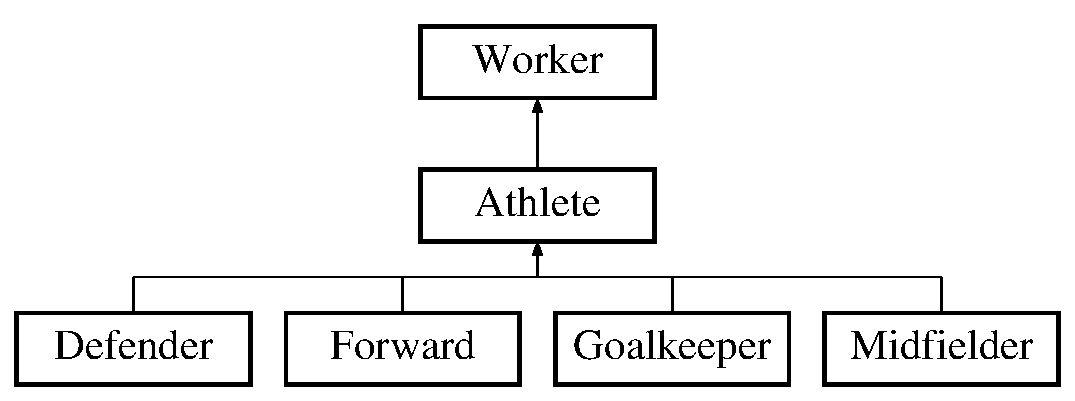
\includegraphics[height=3.000000cm]{class_athlete}
\end{center}
\end{figure}
\subsection*{Public Member Functions}
\begin{DoxyCompactItemize}
\item 
\hyperlink{class_athlete_ae606aa946830e5ea0a05bf8f4fe22132}{Athlete} (string \hyperlink{class_worker_a66cf57341253a31e418cf8abad59ffb1}{name}, \hyperlink{class_date}{Date} \hyperlink{class_worker_a3c1845f40a084b471750a787a87614dd}{birthdate}, unsigned int \hyperlink{class_worker_adfafba55f967994f4595bd914bbba127}{civil\+ID}, unsigned char \hyperlink{class_athlete_a80a64bb1d5c943aaa7ca152d596d9914}{height}, unsigned int \hyperlink{class_worker_afc39287cd510977cfe7697ed2c86b2ca}{id}=0)
\begin{DoxyCompactList}\small\item\em \hyperlink{class_athlete}{Athlete}\textquotesingle{}s Constructor. \end{DoxyCompactList}\item 
\hyperlink{class_athlete_a47d08c02239cf9dec64223ddf7e133fe}{Athlete} (string \&new\+Athlete, \hyperlink{_utils_8hpp_ab91b34ae619fcdfcba4522b4f335bf83}{Position} \hyperlink{class_athlete_ab6c8f0df2238999ed76e563510ac0b38}{position})
\begin{DoxyCompactList}\small\item\em \hyperlink{class_athlete}{Athlete}\textquotesingle{}s Constructor that reads from the athlete\textquotesingle{}s file. \end{DoxyCompactList}\item 
\hyperlink{class_athlete_a8afd915bce6c257a4f512c97fe42a518}{$\sim$\+Athlete} ()
\begin{DoxyCompactList}\small\item\em Destructor. \end{DoxyCompactList}\item 
unsigned int \hyperlink{class_athlete_a18ca289d50900c3825f21d36f2bf8d75}{get\+Position} () const
\begin{DoxyCompactList}\small\item\em Gets the athlete\textquotesingle{}s position. \end{DoxyCompactList}\item 
unsigned int \hyperlink{class_athlete_a54a75ed3943dc6b5e229997be8422466}{get\+Height} () const
\begin{DoxyCompactList}\small\item\em Gets the athlete\textquotesingle{}s height. \end{DoxyCompactList}\item 
\hyperlink{class_e_c_g}{E\+CG} $\ast$ \hyperlink{class_athlete_a9655c13ed4126435df2e57e64884deab}{get\+E\+CG} () const
\begin{DoxyCompactList}\small\item\em Gets the athlete\textquotesingle{}s ecg. \end{DoxyCompactList}\item 
void \hyperlink{class_athlete_a7eda9551e23db1e742a33e9ac61bd42d}{update\+E\+CG} (bool resultado, \hyperlink{class_date}{Date} expiration\+Date)
\begin{DoxyCompactList}\small\item\em Updates the ecg. \end{DoxyCompactList}\item 
bool \hyperlink{class_athlete_a5a6f1744e0944cbabbe333964d6357f4}{is\+Athlete} () const
\begin{DoxyCompactList}\small\item\em Query if this object is athlete. \end{DoxyCompactList}\item 
string \hyperlink{class_athlete_a44a5a7f1676c6ad2faca9bf51877a6f8}{generate\+Info} () const
\begin{DoxyCompactList}\small\item\em Generates the athlete\textquotesingle{}s performance information. \end{DoxyCompactList}\item 
vector$<$ string $>$ \hyperlink{class_athlete_a4c7813bb2b52b7095cb7e85aef2e54d5}{show\+In\+Screen} () const
\begin{DoxyCompactList}\small\item\em Shows all the athlete\textquotesingle{}s information in screen. \end{DoxyCompactList}\item 
void \hyperlink{class_athlete_a73fdec76546be945f02cc2b6d90b99ca}{set\+Birth\+Date} (\hyperlink{class_date}{Date} new\+Birthdate)
\begin{DoxyCompactList}\small\item\em Sets birth date. \end{DoxyCompactList}\item 
void \hyperlink{class_athlete_ab96f3138f984bb830aa69f1502961dc8}{set\+Height} (unsigned int new\+Height)
\begin{DoxyCompactList}\small\item\em Sets the athlete\textquotesingle{}s height. \end{DoxyCompactList}\end{DoxyCompactItemize}
\subsection*{Protected Attributes}
\begin{DoxyCompactItemize}
\item 
unsigned char \hyperlink{class_athlete_a80a64bb1d5c943aaa7ca152d596d9914}{height}
\begin{DoxyCompactList}\small\item\em \hyperlink{class_athlete}{Athlete}\textquotesingle{}s height. \end{DoxyCompactList}\item 
\hyperlink{class_e_c_g}{E\+CG} $\ast$ \hyperlink{class_athlete_aa9576b3d16acdbe4c6efaeed68f690d7}{ecg}
\begin{DoxyCompactList}\small\item\em pointer to ecg when there\textquotesingle{}s an athlete\textquotesingle{}s class. \end{DoxyCompactList}\item 
\hyperlink{_utils_8hpp_ab91b34ae619fcdfcba4522b4f335bf83}{Position} \hyperlink{class_athlete_ab6c8f0df2238999ed76e563510ac0b38}{position}
\begin{DoxyCompactList}\small\item\em \hyperlink{class_athlete}{Athlete}\textquotesingle{}s position. \end{DoxyCompactList}\end{DoxyCompactItemize}
\subsection*{Additional Inherited Members}


\subsection{Detailed Description}
An athlete. 

Luís, 20/11/2016. 

\subsection{Constructor \& Destructor Documentation}
\hypertarget{class_athlete_ae606aa946830e5ea0a05bf8f4fe22132}{}\label{class_athlete_ae606aa946830e5ea0a05bf8f4fe22132} 
\index{Athlete@{Athlete}!Athlete@{Athlete}}
\index{Athlete@{Athlete}!Athlete@{Athlete}}
\subsubsection{\texorpdfstring{Athlete()}{Athlete()}\hspace{0.1cm}{\footnotesize\ttfamily [1/2]}}
{\footnotesize\ttfamily Athlete\+::\+Athlete (\begin{DoxyParamCaption}\item[{string}]{name,  }\item[{\hyperlink{class_date}{Date}}]{birthdate,  }\item[{unsigned int}]{civil\+ID,  }\item[{unsigned char}]{height,  }\item[{unsigned int}]{id = {\ttfamily 0} }\end{DoxyParamCaption})}



\hyperlink{class_athlete}{Athlete}\textquotesingle{}s Constructor. 

Luís, 20/11/2016. 


\begin{DoxyParams}{Parameters}
{\em name} & The name. \\
\hline
{\em birthdate} & The birthdate. \\
\hline
{\em civil\+ID} & Identifier for the civil. \\
\hline
{\em height} & The height. \\
\hline
{\em id} & (Optional) The identifier. \\
\hline
\end{DoxyParams}
\hypertarget{class_athlete_a47d08c02239cf9dec64223ddf7e133fe}{}\label{class_athlete_a47d08c02239cf9dec64223ddf7e133fe} 
\index{Athlete@{Athlete}!Athlete@{Athlete}}
\index{Athlete@{Athlete}!Athlete@{Athlete}}
\subsubsection{\texorpdfstring{Athlete()}{Athlete()}\hspace{0.1cm}{\footnotesize\ttfamily [2/2]}}
{\footnotesize\ttfamily Athlete\+::\+Athlete (\begin{DoxyParamCaption}\item[{string \&}]{new\+Athlete,  }\item[{\hyperlink{_utils_8hpp_ab91b34ae619fcdfcba4522b4f335bf83}{Position}}]{position }\end{DoxyParamCaption})}



\hyperlink{class_athlete}{Athlete}\textquotesingle{}s Constructor that reads from the athlete\textquotesingle{}s file. 

Luís, 20/11/2016. 


\begin{DoxyParams}{Parameters}
{\em new\+Athlete} & \mbox{[}in,out\mbox{]} The new athlete. \\
\hline
{\em position} & The position. \\
\hline
\end{DoxyParams}
\hypertarget{class_athlete_a8afd915bce6c257a4f512c97fe42a518}{}\label{class_athlete_a8afd915bce6c257a4f512c97fe42a518} 
\index{Athlete@{Athlete}!````~Athlete@{$\sim$\+Athlete}}
\index{````~Athlete@{$\sim$\+Athlete}!Athlete@{Athlete}}
\subsubsection{\texorpdfstring{$\sim$\+Athlete()}{~Athlete()}}
{\footnotesize\ttfamily Athlete\+::$\sim$\+Athlete (\begin{DoxyParamCaption}{ }\end{DoxyParamCaption})}



Destructor. 

Luís, 20/11/2016. 

\subsection{Member Function Documentation}
\hypertarget{class_athlete_a44a5a7f1676c6ad2faca9bf51877a6f8}{}\label{class_athlete_a44a5a7f1676c6ad2faca9bf51877a6f8} 
\index{Athlete@{Athlete}!generate\+Info@{generate\+Info}}
\index{generate\+Info@{generate\+Info}!Athlete@{Athlete}}
\subsubsection{\texorpdfstring{generate\+Info()}{generateInfo()}}
{\footnotesize\ttfamily string Athlete\+::generate\+Info (\begin{DoxyParamCaption}{ }\end{DoxyParamCaption}) const\hspace{0.3cm}{\ttfamily [virtual]}}



Generates the athlete\textquotesingle{}s performance information. 

Luís, 20/11/2016. 

\begin{DoxyReturn}{Returns}
The athlete\textquotesingle{}s performance information. 
\end{DoxyReturn}


Reimplemented from \hyperlink{class_worker_ac77905603b86c58cb0a87d6389dca744}{Worker}.

\hypertarget{class_athlete_a9655c13ed4126435df2e57e64884deab}{}\label{class_athlete_a9655c13ed4126435df2e57e64884deab} 
\index{Athlete@{Athlete}!get\+E\+CG@{get\+E\+CG}}
\index{get\+E\+CG@{get\+E\+CG}!Athlete@{Athlete}}
\subsubsection{\texorpdfstring{get\+E\+C\+G()}{getECG()}}
{\footnotesize\ttfamily \hyperlink{class_e_c_g}{E\+CG} $\ast$ Athlete\+::get\+E\+CG (\begin{DoxyParamCaption}{ }\end{DoxyParamCaption}) const\hspace{0.3cm}{\ttfamily [virtual]}}



Gets the athlete\textquotesingle{}s ecg. 

Luís, 20/11/2016. 

\begin{DoxyReturn}{Returns}
Null if it fails, else the ecg. 
\end{DoxyReturn}


Reimplemented from \hyperlink{class_worker_a625cb5da072fd244f38f42e15693058a}{Worker}.

\hypertarget{class_athlete_a54a75ed3943dc6b5e229997be8422466}{}\label{class_athlete_a54a75ed3943dc6b5e229997be8422466} 
\index{Athlete@{Athlete}!get\+Height@{get\+Height}}
\index{get\+Height@{get\+Height}!Athlete@{Athlete}}
\subsubsection{\texorpdfstring{get\+Height()}{getHeight()}}
{\footnotesize\ttfamily unsigned int Athlete\+::get\+Height (\begin{DoxyParamCaption}{ }\end{DoxyParamCaption}) const\hspace{0.3cm}{\ttfamily [virtual]}}



Gets the athlete\textquotesingle{}s height. 

Luís, 20/11/2016. 

\begin{DoxyReturn}{Returns}
The athlete\textquotesingle{}s height. 
\end{DoxyReturn}


Implements \hyperlink{class_worker_a1c5dcdc1c7dc5e498a44f678e964bbfd}{Worker}.

\hypertarget{class_athlete_a18ca289d50900c3825f21d36f2bf8d75}{}\label{class_athlete_a18ca289d50900c3825f21d36f2bf8d75} 
\index{Athlete@{Athlete}!get\+Position@{get\+Position}}
\index{get\+Position@{get\+Position}!Athlete@{Athlete}}
\subsubsection{\texorpdfstring{get\+Position()}{getPosition()}}
{\footnotesize\ttfamily unsigned int Athlete\+::get\+Position (\begin{DoxyParamCaption}{ }\end{DoxyParamCaption}) const\hspace{0.3cm}{\ttfamily [virtual]}}



Gets the athlete\textquotesingle{}s position. 

Luís, 20/11/2016. 

\begin{DoxyReturn}{Returns}
The athlete\textquotesingle{}s position. 
\end{DoxyReturn}


Implements \hyperlink{class_worker_a5fd37dea8c5e6579c1deecbfc1b22db9}{Worker}.

\hypertarget{class_athlete_a5a6f1744e0944cbabbe333964d6357f4}{}\label{class_athlete_a5a6f1744e0944cbabbe333964d6357f4} 
\index{Athlete@{Athlete}!is\+Athlete@{is\+Athlete}}
\index{is\+Athlete@{is\+Athlete}!Athlete@{Athlete}}
\subsubsection{\texorpdfstring{is\+Athlete()}{isAthlete()}}
{\footnotesize\ttfamily bool Athlete\+::is\+Athlete (\begin{DoxyParamCaption}{ }\end{DoxyParamCaption}) const\hspace{0.3cm}{\ttfamily [virtual]}}



Query if this object is athlete. 

Luís, 20/11/2016. 

\begin{DoxyReturn}{Returns}
True if athlete, false if not. 
\end{DoxyReturn}


Implements \hyperlink{class_worker_a0a2eb7505b3a734184be3dfdf3316cc3}{Worker}.

\hypertarget{class_athlete_a73fdec76546be945f02cc2b6d90b99ca}{}\label{class_athlete_a73fdec76546be945f02cc2b6d90b99ca} 
\index{Athlete@{Athlete}!set\+Birth\+Date@{set\+Birth\+Date}}
\index{set\+Birth\+Date@{set\+Birth\+Date}!Athlete@{Athlete}}
\subsubsection{\texorpdfstring{set\+Birth\+Date()}{setBirthDate()}}
{\footnotesize\ttfamily void Athlete\+::set\+Birth\+Date (\begin{DoxyParamCaption}\item[{\hyperlink{class_date}{Date}}]{new\+Birthdate }\end{DoxyParamCaption})\hspace{0.3cm}{\ttfamily [virtual]}}



Sets birth date. 

Luís, 20/11/2016. 


\begin{DoxyParams}{Parameters}
{\em new\+Birthdate} & The new birthdate. \\
\hline
\end{DoxyParams}


Reimplemented from \hyperlink{class_worker_ac48a8315ccdeb2913cd98ea223660f72}{Worker}.

\hypertarget{class_athlete_ab96f3138f984bb830aa69f1502961dc8}{}\label{class_athlete_ab96f3138f984bb830aa69f1502961dc8} 
\index{Athlete@{Athlete}!set\+Height@{set\+Height}}
\index{set\+Height@{set\+Height}!Athlete@{Athlete}}
\subsubsection{\texorpdfstring{set\+Height()}{setHeight()}}
{\footnotesize\ttfamily void Athlete\+::set\+Height (\begin{DoxyParamCaption}\item[{unsigned int}]{new\+Height }\end{DoxyParamCaption})\hspace{0.3cm}{\ttfamily [virtual]}}



Sets the athlete\textquotesingle{}s height. 

Luís, 20/11/2016. 


\begin{DoxyParams}{Parameters}
{\em new\+Height} & New height. \\
\hline
\end{DoxyParams}


Reimplemented from \hyperlink{class_worker_a64124dca31baa9b110779c7698c15a57}{Worker}.

\hypertarget{class_athlete_a4c7813bb2b52b7095cb7e85aef2e54d5}{}\label{class_athlete_a4c7813bb2b52b7095cb7e85aef2e54d5} 
\index{Athlete@{Athlete}!show\+In\+Screen@{show\+In\+Screen}}
\index{show\+In\+Screen@{show\+In\+Screen}!Athlete@{Athlete}}
\subsubsection{\texorpdfstring{show\+In\+Screen()}{showInScreen()}}
{\footnotesize\ttfamily vector$<$ string $>$ Athlete\+::show\+In\+Screen (\begin{DoxyParamCaption}{ }\end{DoxyParamCaption}) const\hspace{0.3cm}{\ttfamily [virtual]}}



Shows all the athlete\textquotesingle{}s information in screen. 

This is a method that shows all the athlete\textquotesingle{}s informaton on the screen

Luís, 20/11/2016. 

\begin{DoxyReturn}{Returns}
A vector of strings; 
\end{DoxyReturn}


Reimplemented from \hyperlink{class_worker_aca1475c72f6e7c6b85114b0bba0da038}{Worker}.

\hypertarget{class_athlete_a7eda9551e23db1e742a33e9ac61bd42d}{}\label{class_athlete_a7eda9551e23db1e742a33e9ac61bd42d} 
\index{Athlete@{Athlete}!update\+E\+CG@{update\+E\+CG}}
\index{update\+E\+CG@{update\+E\+CG}!Athlete@{Athlete}}
\subsubsection{\texorpdfstring{update\+E\+C\+G()}{updateECG()}}
{\footnotesize\ttfamily void Athlete\+::update\+E\+CG (\begin{DoxyParamCaption}\item[{bool}]{resultado,  }\item[{\hyperlink{class_date}{Date}}]{expiration\+Date }\end{DoxyParamCaption})\hspace{0.3cm}{\ttfamily [virtual]}}



Updates the ecg. 

Luís, 20/11/2016. 


\begin{DoxyParams}{Parameters}
{\em resultado} & True to result. \\
\hline
{\em expiration\+Date} & The expiration date. \\
\hline
\end{DoxyParams}


Reimplemented from \hyperlink{class_worker_a7d06c15a1d9872d629988aa054996627}{Worker}.



\subsection{Member Data Documentation}
\hypertarget{class_athlete_aa9576b3d16acdbe4c6efaeed68f690d7}{}\label{class_athlete_aa9576b3d16acdbe4c6efaeed68f690d7} 
\index{Athlete@{Athlete}!ecg@{ecg}}
\index{ecg@{ecg}!Athlete@{Athlete}}
\subsubsection{\texorpdfstring{ecg}{ecg}}
{\footnotesize\ttfamily \hyperlink{class_e_c_g}{E\+CG}$\ast$ Athlete\+::ecg\hspace{0.3cm}{\ttfamily [protected]}}



pointer to ecg when there\textquotesingle{}s an athlete\textquotesingle{}s class. 

\hypertarget{class_athlete_a80a64bb1d5c943aaa7ca152d596d9914}{}\label{class_athlete_a80a64bb1d5c943aaa7ca152d596d9914} 
\index{Athlete@{Athlete}!height@{height}}
\index{height@{height}!Athlete@{Athlete}}
\subsubsection{\texorpdfstring{height}{height}}
{\footnotesize\ttfamily unsigned char Athlete\+::height\hspace{0.3cm}{\ttfamily [protected]}}



\hyperlink{class_athlete}{Athlete}\textquotesingle{}s height. 

\hypertarget{class_athlete_ab6c8f0df2238999ed76e563510ac0b38}{}\label{class_athlete_ab6c8f0df2238999ed76e563510ac0b38} 
\index{Athlete@{Athlete}!position@{position}}
\index{position@{position}!Athlete@{Athlete}}
\subsubsection{\texorpdfstring{position}{position}}
{\footnotesize\ttfamily \hyperlink{_utils_8hpp_ab91b34ae619fcdfcba4522b4f335bf83}{Position} Athlete\+::position\hspace{0.3cm}{\ttfamily [protected]}}



\hyperlink{class_athlete}{Athlete}\textquotesingle{}s position. 



The documentation for this class was generated from the following files\+:\begin{DoxyCompactItemize}
\item 
\hyperlink{_athlete_8hpp}{Athlete.\+hpp}\item 
\hyperlink{_athlete_8cpp}{Athlete.\+cpp}\end{DoxyCompactItemize}

\hypertarget{class_binary_tree}{}\section{Binary\+Tree$<$ T $>$ Class Template Reference}
\label{class_binary_tree}\index{Binary\+Tree$<$ T $>$@{Binary\+Tree$<$ T $>$}}


A binary tree.  




{\ttfamily \#include $<$B\+S\+T.\+h$>$}

\subsection*{Public Member Functions}
\begin{DoxyCompactItemize}
\item 
\hyperlink{class_binary_tree_a9202cce23960faf8f647c6765decccd4}{Binary\+Tree} ()
\begin{DoxyCompactList}\small\item\em Default constructor. \end{DoxyCompactList}\item 
\hyperlink{class_binary_tree_a196a1463712d6f5dfab9e36b26622545}{Binary\+Tree} (const \hyperlink{class_binary_tree}{Binary\+Tree} \&t)
\begin{DoxyCompactList}\small\item\em Copy constructor. \end{DoxyCompactList}\item 
\hyperlink{class_binary_tree_a0e9f40807e8572d3c48ae3c1c97297d9}{Binary\+Tree} (const T \&)
\begin{DoxyCompactList}\small\item\em Constructor. \end{DoxyCompactList}\item 
\hyperlink{class_binary_tree_af4fdef67ba18a1e1839137452fa5b7f3}{Binary\+Tree} (const T \&elem, const \hyperlink{class_binary_tree}{Binary\+Tree} \&esq, const \hyperlink{class_binary_tree}{Binary\+Tree} \&dir)
\begin{DoxyCompactList}\small\item\em Constructor. \end{DoxyCompactList}\item 
\hyperlink{class_binary_tree_a390c319c0b28b958463851119edb8af3}{$\sim$\+Binary\+Tree} ()
\begin{DoxyCompactList}\small\item\em Destructor. \end{DoxyCompactList}\item 
const \hyperlink{class_binary_tree}{Binary\+Tree} \& \hyperlink{class_binary_tree_ac279bcb6977dde769bba27ffba0b1b1f}{operator=} (const \hyperlink{class_binary_tree}{Binary\+Tree} \&rhs)
\begin{DoxyCompactList}\small\item\em Assignment operator. \end{DoxyCompactList}\item 
bool \hyperlink{class_binary_tree_a0d870186995435510057e2b1312e1250}{is\+Empty} () const
\begin{DoxyCompactList}\small\item\em Query if this object is empty. \end{DoxyCompactList}\item 
T \& \hyperlink{class_binary_tree_afe7bd436227bc88b66920abc08ebeaba}{get\+Root} () const
\begin{DoxyCompactList}\small\item\em Gets the root. \end{DoxyCompactList}\item 
void \hyperlink{class_binary_tree_ad72c34cb7d17ae7d3eaaa43bfcc80de3}{make\+Empty} ()
\begin{DoxyCompactList}\small\item\em Makes an empty binary tree. \end{DoxyCompactList}\item 
void \hyperlink{class_binary_tree_a01a8974d6d5f26e03ac0f2fa142a12b2}{output\+Preorder} (ostream \&out) const
\begin{DoxyCompactList}\small\item\em Output preorder. \end{DoxyCompactList}\end{DoxyCompactItemize}
\subsection*{Private Member Functions}
\begin{DoxyCompactItemize}
\item 
void \hyperlink{class_binary_tree_a751ae424bb621e6cf72c53b58174ba5a}{make\+Empty} (\hyperlink{class_b_t_node}{B\+T\+Node}$<$ T $>$ $\ast$r)
\begin{DoxyCompactList}\small\item\em Makes an empty node. \end{DoxyCompactList}\item 
\hyperlink{class_b_t_node}{B\+T\+Node}$<$ T $>$ $\ast$ \hyperlink{class_binary_tree_a014618e17cbd8ec616e95db4c028c60f}{copy\+Subtree} (const \hyperlink{class_b_t_node}{B\+T\+Node}$<$ T $>$ $\ast$n) const
\begin{DoxyCompactList}\small\item\em Copies the subtree described by n. \end{DoxyCompactList}\item 
void \hyperlink{class_binary_tree_a1ffb7f4262ab5f14c76b5bb945c77a8d}{output\+Preorder} (ostream \&out, const \hyperlink{class_b_t_node}{B\+T\+Node}$<$ T $>$ $\ast$n) const
\begin{DoxyCompactList}\small\item\em Output preorder. \end{DoxyCompactList}\end{DoxyCompactItemize}
\subsection*{Private Attributes}
\begin{DoxyCompactItemize}
\item 
\hyperlink{class_b_t_node}{B\+T\+Node}$<$ T $>$ $\ast$ \hyperlink{class_binary_tree_ae587d62783bdf539c98ba7b392be47db}{root}
\begin{DoxyCompactList}\small\item\em The root. \end{DoxyCompactList}\end{DoxyCompactItemize}
\subsection*{Friends}
\begin{DoxyCompactItemize}
\item 
class \hyperlink{class_binary_tree_a803b4f6df7f3239e80af1600d26a7d30}{B\+T\+Itr\+In$<$ T $>$}
\begin{DoxyCompactList}\small\item\em A bt itr in. \end{DoxyCompactList}\item 
class \hyperlink{class_binary_tree_adfe4104666d42d9d6fb4b4ffc1c1fe51}{B\+T\+Itr\+Pre$<$ T $>$}
\begin{DoxyCompactList}\small\item\em A bt itr pre. \end{DoxyCompactList}\item 
class \hyperlink{class_binary_tree_af3c09c804ca3ba21c07c7d7eb41fd606}{B\+T\+Itr\+Post$<$ T $>$}
\begin{DoxyCompactList}\small\item\em A bt itr post. \end{DoxyCompactList}\item 
class \hyperlink{class_binary_tree_aa111eea53d6a1abdc602ea0fc0740878}{B\+T\+Itr\+Level$<$ T $>$}
\begin{DoxyCompactList}\small\item\em A bt itr level. \end{DoxyCompactList}\end{DoxyCompactItemize}


\subsection{Detailed Description}
\subsubsection*{template$<$class T$>$\newline
class Binary\+Tree$<$ T $>$}

A binary tree. 

Lu�s, 20/11/2016. 


\begin{DoxyTemplParams}{Template Parameters}
{\em T} & Generic type parameter. \\
\hline
\end{DoxyTemplParams}


\subsection{Constructor \& Destructor Documentation}
\hypertarget{class_binary_tree_a9202cce23960faf8f647c6765decccd4}{}\label{class_binary_tree_a9202cce23960faf8f647c6765decccd4} 
\index{Binary\+Tree@{Binary\+Tree}!Binary\+Tree@{Binary\+Tree}}
\index{Binary\+Tree@{Binary\+Tree}!Binary\+Tree@{Binary\+Tree}}
\subsubsection{\texorpdfstring{Binary\+Tree()}{BinaryTree()}\hspace{0.1cm}{\footnotesize\ttfamily [1/4]}}
{\footnotesize\ttfamily template$<$class T$>$ \\
\hyperlink{class_binary_tree}{Binary\+Tree}$<$ T $>$\+::\hyperlink{class_binary_tree}{Binary\+Tree} (\begin{DoxyParamCaption}{ }\end{DoxyParamCaption})\hspace{0.3cm}{\ttfamily [inline]}}



Default constructor. 

Lu�s, 20/11/2016. \hypertarget{class_binary_tree_a196a1463712d6f5dfab9e36b26622545}{}\label{class_binary_tree_a196a1463712d6f5dfab9e36b26622545} 
\index{Binary\+Tree@{Binary\+Tree}!Binary\+Tree@{Binary\+Tree}}
\index{Binary\+Tree@{Binary\+Tree}!Binary\+Tree@{Binary\+Tree}}
\subsubsection{\texorpdfstring{Binary\+Tree()}{BinaryTree()}\hspace{0.1cm}{\footnotesize\ttfamily [2/4]}}
{\footnotesize\ttfamily template$<$class T $>$ \\
\hyperlink{class_binary_tree}{Binary\+Tree}$<$ T $>$\+::\hyperlink{class_binary_tree}{Binary\+Tree} (\begin{DoxyParamCaption}\item[{const \hyperlink{class_binary_tree}{Binary\+Tree}$<$ T $>$ \&}]{t }\end{DoxyParamCaption})}



Copy constructor. 

Lu�s, 20/11/2016. 


\begin{DoxyParams}{Parameters}
{\em t} & The \hyperlink{class_binary_tree}{Binary\+Tree} to process. \\
\hline
\end{DoxyParams}
\hypertarget{class_binary_tree_a0e9f40807e8572d3c48ae3c1c97297d9}{}\label{class_binary_tree_a0e9f40807e8572d3c48ae3c1c97297d9} 
\index{Binary\+Tree@{Binary\+Tree}!Binary\+Tree@{Binary\+Tree}}
\index{Binary\+Tree@{Binary\+Tree}!Binary\+Tree@{Binary\+Tree}}
\subsubsection{\texorpdfstring{Binary\+Tree()}{BinaryTree()}\hspace{0.1cm}{\footnotesize\ttfamily [3/4]}}
{\footnotesize\ttfamily template$<$class T$>$ \\
\hyperlink{class_binary_tree}{Binary\+Tree}$<$ T $>$\+::\hyperlink{class_binary_tree}{Binary\+Tree} (\begin{DoxyParamCaption}\item[{const T \&}]{v }\end{DoxyParamCaption})}



Constructor. 

Lu�s, 20/11/2016. 


\begin{DoxyParams}{Parameters}
{\em parameter1} & The first parameter. \\
\hline
\end{DoxyParams}
\hypertarget{class_binary_tree_af4fdef67ba18a1e1839137452fa5b7f3}{}\label{class_binary_tree_af4fdef67ba18a1e1839137452fa5b7f3} 
\index{Binary\+Tree@{Binary\+Tree}!Binary\+Tree@{Binary\+Tree}}
\index{Binary\+Tree@{Binary\+Tree}!Binary\+Tree@{Binary\+Tree}}
\subsubsection{\texorpdfstring{Binary\+Tree()}{BinaryTree()}\hspace{0.1cm}{\footnotesize\ttfamily [4/4]}}
{\footnotesize\ttfamily template$<$class T$>$ \\
\hyperlink{class_binary_tree}{Binary\+Tree}$<$ T $>$\+::\hyperlink{class_binary_tree}{Binary\+Tree} (\begin{DoxyParamCaption}\item[{const T \&}]{elem,  }\item[{const \hyperlink{class_binary_tree}{Binary\+Tree}$<$ T $>$ \&}]{esq,  }\item[{const \hyperlink{class_binary_tree}{Binary\+Tree}$<$ T $>$ \&}]{dir }\end{DoxyParamCaption})}



Constructor. 

Lu�s, 20/11/2016. 


\begin{DoxyParams}{Parameters}
{\em elem} & The element. \\
\hline
{\em esq} & The left node. \\
\hline
{\em dir} & The right node. \\
\hline
\end{DoxyParams}
\hypertarget{class_binary_tree_a390c319c0b28b958463851119edb8af3}{}\label{class_binary_tree_a390c319c0b28b958463851119edb8af3} 
\index{Binary\+Tree@{Binary\+Tree}!````~Binary\+Tree@{$\sim$\+Binary\+Tree}}
\index{````~Binary\+Tree@{$\sim$\+Binary\+Tree}!Binary\+Tree@{Binary\+Tree}}
\subsubsection{\texorpdfstring{$\sim$\+Binary\+Tree()}{~BinaryTree()}}
{\footnotesize\ttfamily template$<$class T$>$ \\
\hyperlink{class_binary_tree}{Binary\+Tree}$<$ T $>$\+::$\sim$\hyperlink{class_binary_tree}{Binary\+Tree} (\begin{DoxyParamCaption}{ }\end{DoxyParamCaption})\hspace{0.3cm}{\ttfamily [inline]}}



Destructor. 

Lu�s, 20/11/2016. 

\subsection{Member Function Documentation}
\hypertarget{class_binary_tree_a014618e17cbd8ec616e95db4c028c60f}{}\label{class_binary_tree_a014618e17cbd8ec616e95db4c028c60f} 
\index{Binary\+Tree@{Binary\+Tree}!copy\+Subtree@{copy\+Subtree}}
\index{copy\+Subtree@{copy\+Subtree}!Binary\+Tree@{Binary\+Tree}}
\subsubsection{\texorpdfstring{copy\+Subtree()}{copySubtree()}}
{\footnotesize\ttfamily template$<$class T$>$ \\
\hyperlink{class_b_t_node}{B\+T\+Node}$<$ T $>$ $\ast$ \hyperlink{class_binary_tree}{Binary\+Tree}$<$ T $>$\+::copy\+Subtree (\begin{DoxyParamCaption}\item[{const \hyperlink{class_b_t_node}{B\+T\+Node}$<$ T $>$ $\ast$}]{n }\end{DoxyParamCaption}) const\hspace{0.3cm}{\ttfamily [private]}}



Copies the subtree described by n. 

Lu�s, 20/11/2016. 


\begin{DoxyParams}{Parameters}
{\em n} & The node to process. \\
\hline
\end{DoxyParams}


\begin{DoxyReturn}{Returns}
Null if it fails, else a pointer to a node; 
\end{DoxyReturn}
\hypertarget{class_binary_tree_afe7bd436227bc88b66920abc08ebeaba}{}\label{class_binary_tree_afe7bd436227bc88b66920abc08ebeaba} 
\index{Binary\+Tree@{Binary\+Tree}!get\+Root@{get\+Root}}
\index{get\+Root@{get\+Root}!Binary\+Tree@{Binary\+Tree}}
\subsubsection{\texorpdfstring{get\+Root()}{getRoot()}}
{\footnotesize\ttfamily template$<$class T$>$ \\
T\& \hyperlink{class_binary_tree}{Binary\+Tree}$<$ T $>$\+::get\+Root (\begin{DoxyParamCaption}{ }\end{DoxyParamCaption}) const\hspace{0.3cm}{\ttfamily [inline]}}



Gets the root. 

Lu�s, 20/11/2016. 


\begin{DoxyExceptions}{Exceptions}
{\em \hyperlink{class_underflow}{Underflow}} & Thrown when an underflow error condition occurs. \\
\hline
\end{DoxyExceptions}


\begin{DoxyReturn}{Returns}
The root. 
\end{DoxyReturn}
\hypertarget{class_binary_tree_a0d870186995435510057e2b1312e1250}{}\label{class_binary_tree_a0d870186995435510057e2b1312e1250} 
\index{Binary\+Tree@{Binary\+Tree}!is\+Empty@{is\+Empty}}
\index{is\+Empty@{is\+Empty}!Binary\+Tree@{Binary\+Tree}}
\subsubsection{\texorpdfstring{is\+Empty()}{isEmpty()}}
{\footnotesize\ttfamily template$<$class T$>$ \\
bool \hyperlink{class_binary_tree}{Binary\+Tree}$<$ T $>$\+::is\+Empty (\begin{DoxyParamCaption}{ }\end{DoxyParamCaption}) const\hspace{0.3cm}{\ttfamily [inline]}}



Query if this object is empty. 

Lu�s, 20/11/2016. 

\begin{DoxyReturn}{Returns}
True if empty, false if not. 
\end{DoxyReturn}
\hypertarget{class_binary_tree_ad72c34cb7d17ae7d3eaaa43bfcc80de3}{}\label{class_binary_tree_ad72c34cb7d17ae7d3eaaa43bfcc80de3} 
\index{Binary\+Tree@{Binary\+Tree}!make\+Empty@{make\+Empty}}
\index{make\+Empty@{make\+Empty}!Binary\+Tree@{Binary\+Tree}}
\subsubsection{\texorpdfstring{make\+Empty()}{makeEmpty()}\hspace{0.1cm}{\footnotesize\ttfamily [1/2]}}
{\footnotesize\ttfamily template$<$class T $>$ \\
void \hyperlink{class_binary_tree}{Binary\+Tree}$<$ T $>$\+::make\+Empty (\begin{DoxyParamCaption}{ }\end{DoxyParamCaption})}



Makes an empty binary tree. 

Lu�s, 20/11/2016. \hypertarget{class_binary_tree_a751ae424bb621e6cf72c53b58174ba5a}{}\label{class_binary_tree_a751ae424bb621e6cf72c53b58174ba5a} 
\index{Binary\+Tree@{Binary\+Tree}!make\+Empty@{make\+Empty}}
\index{make\+Empty@{make\+Empty}!Binary\+Tree@{Binary\+Tree}}
\subsubsection{\texorpdfstring{make\+Empty()}{makeEmpty()}\hspace{0.1cm}{\footnotesize\ttfamily [2/2]}}
{\footnotesize\ttfamily template$<$class T$>$ \\
void \hyperlink{class_binary_tree}{Binary\+Tree}$<$ T $>$\+::make\+Empty (\begin{DoxyParamCaption}\item[{\hyperlink{class_b_t_node}{B\+T\+Node}$<$ T $>$ $\ast$}]{r }\end{DoxyParamCaption})\hspace{0.3cm}{\ttfamily [private]}}



Makes an empty node. 

Lu�s, 20/11/2016. 


\begin{DoxyParams}{Parameters}
{\em r} & \mbox{[}in,out\mbox{]} If non-\/null, binary tree node pointer to process. \\
\hline
\end{DoxyParams}
\hypertarget{class_binary_tree_ac279bcb6977dde769bba27ffba0b1b1f}{}\label{class_binary_tree_ac279bcb6977dde769bba27ffba0b1b1f} 
\index{Binary\+Tree@{Binary\+Tree}!operator=@{operator=}}
\index{operator=@{operator=}!Binary\+Tree@{Binary\+Tree}}
\subsubsection{\texorpdfstring{operator=()}{operator=()}}
{\footnotesize\ttfamily template$<$class T $>$ \\
const \hyperlink{class_binary_tree}{Binary\+Tree}$<$ T $>$ \& \hyperlink{class_binary_tree}{Binary\+Tree}$<$ T $>$\+::operator= (\begin{DoxyParamCaption}\item[{const \hyperlink{class_binary_tree}{Binary\+Tree}$<$ T $>$ \&}]{rhs }\end{DoxyParamCaption})}



Assignment operator. 

Lu�s, 20/11/2016. 


\begin{DoxyParams}{Parameters}
{\em rhs} & The right hand side. \\
\hline
\end{DoxyParams}


\begin{DoxyReturn}{Returns}
A shallow copy of this object. 
\end{DoxyReturn}
\hypertarget{class_binary_tree_a01a8974d6d5f26e03ac0f2fa142a12b2}{}\label{class_binary_tree_a01a8974d6d5f26e03ac0f2fa142a12b2} 
\index{Binary\+Tree@{Binary\+Tree}!output\+Preorder@{output\+Preorder}}
\index{output\+Preorder@{output\+Preorder}!Binary\+Tree@{Binary\+Tree}}
\subsubsection{\texorpdfstring{output\+Preorder()}{outputPreorder()}\hspace{0.1cm}{\footnotesize\ttfamily [1/2]}}
{\footnotesize\ttfamily template$<$class T $>$ \\
void \hyperlink{class_binary_tree}{Binary\+Tree}$<$ T $>$\+::output\+Preorder (\begin{DoxyParamCaption}\item[{ostream \&}]{out }\end{DoxyParamCaption}) const}



Output preorder. 

Lu�s, 20/11/2016. 


\begin{DoxyParams}{Parameters}
{\em out} & \mbox{[}in,out\mbox{]} The outfile. \\
\hline
\end{DoxyParams}
\hypertarget{class_binary_tree_a1ffb7f4262ab5f14c76b5bb945c77a8d}{}\label{class_binary_tree_a1ffb7f4262ab5f14c76b5bb945c77a8d} 
\index{Binary\+Tree@{Binary\+Tree}!output\+Preorder@{output\+Preorder}}
\index{output\+Preorder@{output\+Preorder}!Binary\+Tree@{Binary\+Tree}}
\subsubsection{\texorpdfstring{output\+Preorder()}{outputPreorder()}\hspace{0.1cm}{\footnotesize\ttfamily [2/2]}}
{\footnotesize\ttfamily template$<$class T$>$ \\
void \hyperlink{class_binary_tree}{Binary\+Tree}$<$ T $>$\+::output\+Preorder (\begin{DoxyParamCaption}\item[{ostream \&}]{out,  }\item[{const \hyperlink{class_b_t_node}{B\+T\+Node}$<$ T $>$ $\ast$}]{n }\end{DoxyParamCaption}) const\hspace{0.3cm}{\ttfamily [private]}}



Output preorder. 

Lu�s, 20/11/2016. 


\begin{DoxyParams}{Parameters}
{\em out} & \mbox{[}in,out\mbox{]} The outfile. \\
\hline
{\em n} & The node pointer to process. \\
\hline
\end{DoxyParams}


\subsection{Friends And Related Function Documentation}
\hypertarget{class_binary_tree_a803b4f6df7f3239e80af1600d26a7d30}{}\label{class_binary_tree_a803b4f6df7f3239e80af1600d26a7d30} 
\index{Binary\+Tree@{Binary\+Tree}!B\+T\+Itr\+In$<$ T $>$@{B\+T\+Itr\+In$<$ T $>$}}
\index{B\+T\+Itr\+In$<$ T $>$@{B\+T\+Itr\+In$<$ T $>$}!Binary\+Tree@{Binary\+Tree}}
\subsubsection{\texorpdfstring{B\+T\+Itr\+In$<$ T $>$}{BTItrIn< T >}}
{\footnotesize\ttfamily template$<$class T$>$ \\
friend class \hyperlink{class_b_t_itr_in}{B\+T\+Itr\+In}$<$ T $>$\hspace{0.3cm}{\ttfamily [friend]}}



A bt itr in. 

Lu�s, 20/11/2016. 


\begin{DoxyTemplParams}{Template Parameters}
{\em T} & Generic type parameter. \\
\hline
\end{DoxyTemplParams}
\hypertarget{class_binary_tree_aa111eea53d6a1abdc602ea0fc0740878}{}\label{class_binary_tree_aa111eea53d6a1abdc602ea0fc0740878} 
\index{Binary\+Tree@{Binary\+Tree}!B\+T\+Itr\+Level$<$ T $>$@{B\+T\+Itr\+Level$<$ T $>$}}
\index{B\+T\+Itr\+Level$<$ T $>$@{B\+T\+Itr\+Level$<$ T $>$}!Binary\+Tree@{Binary\+Tree}}
\subsubsection{\texorpdfstring{B\+T\+Itr\+Level$<$ T $>$}{BTItrLevel< T >}}
{\footnotesize\ttfamily template$<$class T$>$ \\
friend class \hyperlink{class_b_t_itr_level}{B\+T\+Itr\+Level}$<$ T $>$\hspace{0.3cm}{\ttfamily [friend]}}



A bt itr level. 

Lu�s, 20/11/2016. 


\begin{DoxyTemplParams}{Template Parameters}
{\em T} & Generic type parameter. \\
\hline
\end{DoxyTemplParams}
\hypertarget{class_binary_tree_af3c09c804ca3ba21c07c7d7eb41fd606}{}\label{class_binary_tree_af3c09c804ca3ba21c07c7d7eb41fd606} 
\index{Binary\+Tree@{Binary\+Tree}!B\+T\+Itr\+Post$<$ T $>$@{B\+T\+Itr\+Post$<$ T $>$}}
\index{B\+T\+Itr\+Post$<$ T $>$@{B\+T\+Itr\+Post$<$ T $>$}!Binary\+Tree@{Binary\+Tree}}
\subsubsection{\texorpdfstring{B\+T\+Itr\+Post$<$ T $>$}{BTItrPost< T >}}
{\footnotesize\ttfamily template$<$class T$>$ \\
friend class \hyperlink{class_b_t_itr_post}{B\+T\+Itr\+Post}$<$ T $>$\hspace{0.3cm}{\ttfamily [friend]}}



A bt itr post. 

Lu�s, 20/11/2016. 


\begin{DoxyTemplParams}{Template Parameters}
{\em T} & Generic type parameter. \\
\hline
\end{DoxyTemplParams}
\hypertarget{class_binary_tree_adfe4104666d42d9d6fb4b4ffc1c1fe51}{}\label{class_binary_tree_adfe4104666d42d9d6fb4b4ffc1c1fe51} 
\index{Binary\+Tree@{Binary\+Tree}!B\+T\+Itr\+Pre$<$ T $>$@{B\+T\+Itr\+Pre$<$ T $>$}}
\index{B\+T\+Itr\+Pre$<$ T $>$@{B\+T\+Itr\+Pre$<$ T $>$}!Binary\+Tree@{Binary\+Tree}}
\subsubsection{\texorpdfstring{B\+T\+Itr\+Pre$<$ T $>$}{BTItrPre< T >}}
{\footnotesize\ttfamily template$<$class T$>$ \\
friend class \hyperlink{class_b_t_itr_pre}{B\+T\+Itr\+Pre}$<$ T $>$\hspace{0.3cm}{\ttfamily [friend]}}



A bt itr pre. 

Lu�s, 20/11/2016. 


\begin{DoxyTemplParams}{Template Parameters}
{\em T} & Generic type parameter. \\
\hline
\end{DoxyTemplParams}


\subsection{Member Data Documentation}
\hypertarget{class_binary_tree_ae587d62783bdf539c98ba7b392be47db}{}\label{class_binary_tree_ae587d62783bdf539c98ba7b392be47db} 
\index{Binary\+Tree@{Binary\+Tree}!root@{root}}
\index{root@{root}!Binary\+Tree@{Binary\+Tree}}
\subsubsection{\texorpdfstring{root}{root}}
{\footnotesize\ttfamily template$<$class T$>$ \\
\hyperlink{class_b_t_node}{B\+T\+Node}$<$T$>$$\ast$ \hyperlink{class_binary_tree}{Binary\+Tree}$<$ T $>$\+::root\hspace{0.3cm}{\ttfamily [private]}}



The root. 



The documentation for this class was generated from the following file\+:\begin{DoxyCompactItemize}
\item 
\hyperlink{_b_s_t_8h}{B\+S\+T.\+h}\end{DoxyCompactItemize}

\hypertarget{class_b_t_itr_in}{}\section{B\+T\+Itr\+In$<$ T $>$ Class Template Reference}
\label{class_b_t_itr_in}\index{B\+T\+Itr\+In$<$ T $>$@{B\+T\+Itr\+In$<$ T $>$}}


An in binary tree iterator.  




{\ttfamily \#include $<$B\+S\+T.\+h$>$}

\subsection*{Public Member Functions}
\begin{DoxyCompactItemize}
\item 
\hyperlink{class_b_t_itr_in_a97695772bf055a51e72523695ad6e138}{B\+T\+Itr\+In} (const \hyperlink{class_binary_tree}{Binary\+Tree}$<$ T $>$ \&bt)
\begin{DoxyCompactList}\small\item\em Constructor. \end{DoxyCompactList}\item 
void \hyperlink{class_b_t_itr_in_a4f5a9d36fe927d076d0d566d7c14582a}{advance} ()
\begin{DoxyCompactList}\small\item\em Advances this object. \end{DoxyCompactList}\item 
T \& \hyperlink{class_b_t_itr_in_a0fbe544d77133bbddf008685f9d95bdc}{retrieve} ()
\begin{DoxyCompactList}\small\item\em Retrieves a reference to a T. \end{DoxyCompactList}\item 
bool \hyperlink{class_b_t_itr_in_ad244b304d9bd2570c7d6d2ca557212a4}{is\+At\+End} ()
\begin{DoxyCompactList}\small\item\em Query if this object is at end. \end{DoxyCompactList}\end{DoxyCompactItemize}
\subsection*{Private Member Functions}
\begin{DoxyCompactItemize}
\item 
void \hyperlink{class_b_t_itr_in_a97a517be39439aa958384e0868fe46a3}{slide\+Left} (\hyperlink{class_b_t_node}{B\+T\+Node}$<$ T $>$ $\ast$n)
\begin{DoxyCompactList}\small\item\em Slide left. \end{DoxyCompactList}\end{DoxyCompactItemize}
\subsection*{Private Attributes}
\begin{DoxyCompactItemize}
\item 
stack$<$ \hyperlink{class_b_t_node}{B\+T\+Node}$<$ T $>$ $\ast$ $>$ \hyperlink{class_b_t_itr_in_aa50afea931b98eaa5c5d6d8cc8eb82fe}{itr\+Stack}
\begin{DoxyCompactList}\small\item\em Stack of itrs. \end{DoxyCompactList}\end{DoxyCompactItemize}


\subsection{Detailed Description}
\subsubsection*{template$<$class T$>$\newline
class B\+T\+Itr\+In$<$ T $>$}

An in binary tree iterator. 

Lu�s, 20/11/2016. 


\begin{DoxyTemplParams}{Template Parameters}
{\em T} & Generic type parameter. \\
\hline
\end{DoxyTemplParams}


Lu�s, 20/11/2016. 

\subsection{Constructor \& Destructor Documentation}
\hypertarget{class_b_t_itr_in_a97695772bf055a51e72523695ad6e138}{}\label{class_b_t_itr_in_a97695772bf055a51e72523695ad6e138} 
\index{B\+T\+Itr\+In@{B\+T\+Itr\+In}!B\+T\+Itr\+In@{B\+T\+Itr\+In}}
\index{B\+T\+Itr\+In@{B\+T\+Itr\+In}!B\+T\+Itr\+In@{B\+T\+Itr\+In}}
\subsubsection{\texorpdfstring{B\+T\+Itr\+In()}{BTItrIn()}}
{\footnotesize\ttfamily template$<$class T $>$ \\
\hyperlink{class_b_t_itr_in}{B\+T\+Itr\+In}$<$ T $>$\+::\hyperlink{class_b_t_itr_in}{B\+T\+Itr\+In} (\begin{DoxyParamCaption}\item[{const \hyperlink{class_binary_tree}{Binary\+Tree}$<$ T $>$ \&}]{bt }\end{DoxyParamCaption})}



Constructor. 

Lu�s, 20/11/2016. 


\begin{DoxyParams}{Parameters}
{\em bt} & The binary tree. \\
\hline
\end{DoxyParams}


\subsection{Member Function Documentation}
\hypertarget{class_b_t_itr_in_a4f5a9d36fe927d076d0d566d7c14582a}{}\label{class_b_t_itr_in_a4f5a9d36fe927d076d0d566d7c14582a} 
\index{B\+T\+Itr\+In@{B\+T\+Itr\+In}!advance@{advance}}
\index{advance@{advance}!B\+T\+Itr\+In@{B\+T\+Itr\+In}}
\subsubsection{\texorpdfstring{advance()}{advance()}}
{\footnotesize\ttfamily template$<$class T $>$ \\
void \hyperlink{class_b_t_itr_in}{B\+T\+Itr\+In}$<$ T $>$\+::advance (\begin{DoxyParamCaption}{ }\end{DoxyParamCaption})}



Advances this object. 

Lu�s, 20/11/2016. \hypertarget{class_b_t_itr_in_ad244b304d9bd2570c7d6d2ca557212a4}{}\label{class_b_t_itr_in_ad244b304d9bd2570c7d6d2ca557212a4} 
\index{B\+T\+Itr\+In@{B\+T\+Itr\+In}!is\+At\+End@{is\+At\+End}}
\index{is\+At\+End@{is\+At\+End}!B\+T\+Itr\+In@{B\+T\+Itr\+In}}
\subsubsection{\texorpdfstring{is\+At\+End()}{isAtEnd()}}
{\footnotesize\ttfamily template$<$class T $>$ \\
bool \hyperlink{class_b_t_itr_in}{B\+T\+Itr\+In}$<$ T $>$\+::is\+At\+End (\begin{DoxyParamCaption}{ }\end{DoxyParamCaption})\hspace{0.3cm}{\ttfamily [inline]}}



Query if this object is at end. 

Lu�s, 20/11/2016. 

\begin{DoxyReturn}{Returns}
True if at end, false if not. 
\end{DoxyReturn}
\hypertarget{class_b_t_itr_in_a0fbe544d77133bbddf008685f9d95bdc}{}\label{class_b_t_itr_in_a0fbe544d77133bbddf008685f9d95bdc} 
\index{B\+T\+Itr\+In@{B\+T\+Itr\+In}!retrieve@{retrieve}}
\index{retrieve@{retrieve}!B\+T\+Itr\+In@{B\+T\+Itr\+In}}
\subsubsection{\texorpdfstring{retrieve()}{retrieve()}}
{\footnotesize\ttfamily template$<$class T $>$ \\
T\& \hyperlink{class_b_t_itr_in}{B\+T\+Itr\+In}$<$ T $>$\+::retrieve (\begin{DoxyParamCaption}{ }\end{DoxyParamCaption})\hspace{0.3cm}{\ttfamily [inline]}}



Retrieves a reference to a T. 

Lu�s, 20/11/2016. 

\begin{DoxyReturn}{Returns}
A reference to a T. 
\end{DoxyReturn}
\hypertarget{class_b_t_itr_in_a97a517be39439aa958384e0868fe46a3}{}\label{class_b_t_itr_in_a97a517be39439aa958384e0868fe46a3} 
\index{B\+T\+Itr\+In@{B\+T\+Itr\+In}!slide\+Left@{slide\+Left}}
\index{slide\+Left@{slide\+Left}!B\+T\+Itr\+In@{B\+T\+Itr\+In}}
\subsubsection{\texorpdfstring{slide\+Left()}{slideLeft()}}
{\footnotesize\ttfamily template$<$class T $>$ \\
void \hyperlink{class_b_t_itr_in}{B\+T\+Itr\+In}$<$ T $>$\+::slide\+Left (\begin{DoxyParamCaption}\item[{\hyperlink{class_b_t_node}{B\+T\+Node}$<$ T $>$ $\ast$}]{n }\end{DoxyParamCaption})\hspace{0.3cm}{\ttfamily [private]}}



Slide left. 

Lu�s, 20/11/2016. 


\begin{DoxyParams}{Parameters}
{\em n} & \mbox{[}in,out\mbox{]} If non-\/null, the \hyperlink{class_b_t_node}{B\+T\+Node}$<$T$>$ to process. \\
\hline
\end{DoxyParams}


\subsection{Member Data Documentation}
\hypertarget{class_b_t_itr_in_aa50afea931b98eaa5c5d6d8cc8eb82fe}{}\label{class_b_t_itr_in_aa50afea931b98eaa5c5d6d8cc8eb82fe} 
\index{B\+T\+Itr\+In@{B\+T\+Itr\+In}!itr\+Stack@{itr\+Stack}}
\index{itr\+Stack@{itr\+Stack}!B\+T\+Itr\+In@{B\+T\+Itr\+In}}
\subsubsection{\texorpdfstring{itr\+Stack}{itrStack}}
{\footnotesize\ttfamily template$<$class T $>$ \\
stack$<$\hyperlink{class_b_t_node}{B\+T\+Node}$<$T$>$ $\ast$$>$ \hyperlink{class_b_t_itr_in}{B\+T\+Itr\+In}$<$ T $>$\+::itr\+Stack\hspace{0.3cm}{\ttfamily [private]}}



Stack of itrs. 



The documentation for this class was generated from the following file\+:\begin{DoxyCompactItemize}
\item 
\hyperlink{_b_s_t_8h}{B\+S\+T.\+h}\end{DoxyCompactItemize}

\hypertarget{class_b_t_itr_level}{}\section{B\+T\+Itr\+Level$<$ T $>$ Class Template Reference}
\label{class_b_t_itr_level}\index{B\+T\+Itr\+Level$<$ T $>$@{B\+T\+Itr\+Level$<$ T $>$}}


A level binary tree iterator.  




{\ttfamily \#include $<$B\+S\+T.\+h$>$}

\subsection*{Public Member Functions}
\begin{DoxyCompactItemize}
\item 
\hyperlink{class_b_t_itr_level_a9973e6775bfa77ec8627d3a7b238ff18}{B\+T\+Itr\+Level} (const \hyperlink{class_binary_tree}{Binary\+Tree}$<$ T $>$ \&bt)
\begin{DoxyCompactList}\small\item\em Constructor. \end{DoxyCompactList}\item 
void \hyperlink{class_b_t_itr_level_ac8ce8142bece1f85e6f0a2680dc10521}{advance} ()
\begin{DoxyCompactList}\small\item\em Advances this object. \end{DoxyCompactList}\item 
T \& \hyperlink{class_b_t_itr_level_a827ba7cfbc59ecd9620d0dfc85091c55}{retrieve} ()
\begin{DoxyCompactList}\small\item\em Retrieves a reference to a T. \end{DoxyCompactList}\item 
\hyperlink{class_b_t_node}{B\+T\+Node}$<$ T $>$ $\ast$ \hyperlink{class_b_t_itr_level_a244e59c5a0ac8ef22f0f8f011382d0ed}{get\+Node} () const
\begin{DoxyCompactList}\small\item\em Gets the node. \end{DoxyCompactList}\item 
bool \hyperlink{class_b_t_itr_level_ac612118afbbb777f0093bc08345e7b37}{is\+At\+End} ()
\begin{DoxyCompactList}\small\item\em Query if this object is at end. \end{DoxyCompactList}\end{DoxyCompactItemize}
\subsection*{Private Attributes}
\begin{DoxyCompactItemize}
\item 
queue$<$ \hyperlink{class_b_t_node}{B\+T\+Node}$<$ T $>$ $\ast$ $>$ \hyperlink{class_b_t_itr_level_a2492422e798ffbb71d65744167bf7dab}{itr\+Queue}
\begin{DoxyCompactList}\small\item\em Queue of itrs. \end{DoxyCompactList}\end{DoxyCompactItemize}


\subsection{Detailed Description}
\subsubsection*{template$<$class T$>$\newline
class B\+T\+Itr\+Level$<$ T $>$}

A level binary tree iterator. 

Lu�s, 20/11/2016. 


\begin{DoxyTemplParams}{Template Parameters}
{\em T} & Generic type parameter. \\
\hline
\end{DoxyTemplParams}


\subsection{Constructor \& Destructor Documentation}
\hypertarget{class_b_t_itr_level_a9973e6775bfa77ec8627d3a7b238ff18}{}\label{class_b_t_itr_level_a9973e6775bfa77ec8627d3a7b238ff18} 
\index{B\+T\+Itr\+Level@{B\+T\+Itr\+Level}!B\+T\+Itr\+Level@{B\+T\+Itr\+Level}}
\index{B\+T\+Itr\+Level@{B\+T\+Itr\+Level}!B\+T\+Itr\+Level@{B\+T\+Itr\+Level}}
\subsubsection{\texorpdfstring{B\+T\+Itr\+Level()}{BTItrLevel()}}
{\footnotesize\ttfamily template$<$class T $>$ \\
\hyperlink{class_b_t_itr_level}{B\+T\+Itr\+Level}$<$ T $>$\+::\hyperlink{class_b_t_itr_level}{B\+T\+Itr\+Level} (\begin{DoxyParamCaption}\item[{const \hyperlink{class_binary_tree}{Binary\+Tree}$<$ T $>$ \&}]{bt }\end{DoxyParamCaption})}



Constructor. 

Lu�s, 20/11/2016. 


\begin{DoxyParams}{Parameters}
{\em bt} & The bt. \\
\hline
\end{DoxyParams}


\subsection{Member Function Documentation}
\hypertarget{class_b_t_itr_level_ac8ce8142bece1f85e6f0a2680dc10521}{}\label{class_b_t_itr_level_ac8ce8142bece1f85e6f0a2680dc10521} 
\index{B\+T\+Itr\+Level@{B\+T\+Itr\+Level}!advance@{advance}}
\index{advance@{advance}!B\+T\+Itr\+Level@{B\+T\+Itr\+Level}}
\subsubsection{\texorpdfstring{advance()}{advance()}}
{\footnotesize\ttfamily template$<$class T $>$ \\
void \hyperlink{class_b_t_itr_level}{B\+T\+Itr\+Level}$<$ T $>$\+::advance (\begin{DoxyParamCaption}{ }\end{DoxyParamCaption})}



Advances this object. 

Lu�s, 20/11/2016. \hypertarget{class_b_t_itr_level_a244e59c5a0ac8ef22f0f8f011382d0ed}{}\label{class_b_t_itr_level_a244e59c5a0ac8ef22f0f8f011382d0ed} 
\index{B\+T\+Itr\+Level@{B\+T\+Itr\+Level}!get\+Node@{get\+Node}}
\index{get\+Node@{get\+Node}!B\+T\+Itr\+Level@{B\+T\+Itr\+Level}}
\subsubsection{\texorpdfstring{get\+Node()}{getNode()}}
{\footnotesize\ttfamily template$<$class T $>$ \\
\hyperlink{class_b_t_node}{B\+T\+Node}$<$T$>$$\ast$ \hyperlink{class_b_t_itr_level}{B\+T\+Itr\+Level}$<$ T $>$\+::get\+Node (\begin{DoxyParamCaption}{ }\end{DoxyParamCaption}) const\hspace{0.3cm}{\ttfamily [inline]}}



Gets the node. 

Lu�s, 20/11/2016. 

\begin{DoxyReturn}{Returns}
Null if it fails, else the node. 
\end{DoxyReturn}
\hypertarget{class_b_t_itr_level_ac612118afbbb777f0093bc08345e7b37}{}\label{class_b_t_itr_level_ac612118afbbb777f0093bc08345e7b37} 
\index{B\+T\+Itr\+Level@{B\+T\+Itr\+Level}!is\+At\+End@{is\+At\+End}}
\index{is\+At\+End@{is\+At\+End}!B\+T\+Itr\+Level@{B\+T\+Itr\+Level}}
\subsubsection{\texorpdfstring{is\+At\+End()}{isAtEnd()}}
{\footnotesize\ttfamily template$<$class T $>$ \\
bool \hyperlink{class_b_t_itr_level}{B\+T\+Itr\+Level}$<$ T $>$\+::is\+At\+End (\begin{DoxyParamCaption}{ }\end{DoxyParamCaption})\hspace{0.3cm}{\ttfamily [inline]}}



Query if this object is at end. 

Lu�s, 20/11/2016. 

\begin{DoxyReturn}{Returns}
True if at end, false if not. 
\end{DoxyReturn}
\hypertarget{class_b_t_itr_level_a827ba7cfbc59ecd9620d0dfc85091c55}{}\label{class_b_t_itr_level_a827ba7cfbc59ecd9620d0dfc85091c55} 
\index{B\+T\+Itr\+Level@{B\+T\+Itr\+Level}!retrieve@{retrieve}}
\index{retrieve@{retrieve}!B\+T\+Itr\+Level@{B\+T\+Itr\+Level}}
\subsubsection{\texorpdfstring{retrieve()}{retrieve()}}
{\footnotesize\ttfamily template$<$class T $>$ \\
T\& \hyperlink{class_b_t_itr_level}{B\+T\+Itr\+Level}$<$ T $>$\+::retrieve (\begin{DoxyParamCaption}{ }\end{DoxyParamCaption})\hspace{0.3cm}{\ttfamily [inline]}}



Retrieves a reference to a T. 

Lu�s, 20/11/2016. 

\begin{DoxyReturn}{Returns}
A reference to a T. 
\end{DoxyReturn}


\subsection{Member Data Documentation}
\hypertarget{class_b_t_itr_level_a2492422e798ffbb71d65744167bf7dab}{}\label{class_b_t_itr_level_a2492422e798ffbb71d65744167bf7dab} 
\index{B\+T\+Itr\+Level@{B\+T\+Itr\+Level}!itr\+Queue@{itr\+Queue}}
\index{itr\+Queue@{itr\+Queue}!B\+T\+Itr\+Level@{B\+T\+Itr\+Level}}
\subsubsection{\texorpdfstring{itr\+Queue}{itrQueue}}
{\footnotesize\ttfamily template$<$class T $>$ \\
queue$<$\hyperlink{class_b_t_node}{B\+T\+Node}$<$T$>$ $\ast$$>$ \hyperlink{class_b_t_itr_level}{B\+T\+Itr\+Level}$<$ T $>$\+::itr\+Queue\hspace{0.3cm}{\ttfamily [private]}}



Queue of itrs. 



The documentation for this class was generated from the following file\+:\begin{DoxyCompactItemize}
\item 
\hyperlink{_b_s_t_8h}{B\+S\+T.\+h}\end{DoxyCompactItemize}

\hypertarget{class_b_t_itr_post}{}\section{B\+T\+Itr\+Post$<$ T $>$ Class Template Reference}
\label{class_b_t_itr_post}\index{B\+T\+Itr\+Post$<$ T $>$@{B\+T\+Itr\+Post$<$ T $>$}}


A post binary tree iterator.  




{\ttfamily \#include $<$B\+S\+T.\+h$>$}

\subsection*{Public Member Functions}
\begin{DoxyCompactItemize}
\item 
\hyperlink{class_b_t_itr_post_a52b3ebaefe70085321204f69db9449e7}{B\+T\+Itr\+Post} (const \hyperlink{class_binary_tree}{Binary\+Tree}$<$ T $>$ \&bt)
\begin{DoxyCompactList}\small\item\em Constructor. \end{DoxyCompactList}\item 
void \hyperlink{class_b_t_itr_post_abe3a1f620e4122aa6c5d2ba120465ace}{advance} ()
\begin{DoxyCompactList}\small\item\em Advances this object. \end{DoxyCompactList}\item 
T \& \hyperlink{class_b_t_itr_post_ae3578aa6f427291651f51ab5d7305dbd}{retrieve} ()
\begin{DoxyCompactList}\small\item\em Retrieves a reference to a T. \end{DoxyCompactList}\item 
bool \hyperlink{class_b_t_itr_post_ad3ab7ee3ff8897eff2f2ee2971c452d8}{is\+At\+End} ()
\begin{DoxyCompactList}\small\item\em Query if this object is at end. \end{DoxyCompactList}\end{DoxyCompactItemize}
\subsection*{Private Member Functions}
\begin{DoxyCompactItemize}
\item 
void \hyperlink{class_b_t_itr_post_aeb538575d0d9e74c15e856d4ec7c2afc}{slide\+Down} (\hyperlink{class_b_t_node}{B\+T\+Node}$<$ T $>$ $\ast$n)
\begin{DoxyCompactList}\small\item\em Slide down. \end{DoxyCompactList}\end{DoxyCompactItemize}
\subsection*{Private Attributes}
\begin{DoxyCompactItemize}
\item 
stack$<$ \hyperlink{class_b_t_node}{B\+T\+Node}$<$ T $>$ $\ast$ $>$ \hyperlink{class_b_t_itr_post_ae6749ceccbea8e413da53a0ab5b150c5}{itr\+Stack}
\begin{DoxyCompactList}\small\item\em Stack of itrs. \end{DoxyCompactList}\item 
stack$<$ bool $>$ \hyperlink{class_b_t_itr_post_aa5f0b8f3427dcff09eda7a83fb0ba963}{visit\+Stack}
\begin{DoxyCompactList}\small\item\em Stack of visits. \end{DoxyCompactList}\end{DoxyCompactItemize}


\subsection{Detailed Description}
\subsubsection*{template$<$class T$>$\newline
class B\+T\+Itr\+Post$<$ T $>$}

A post binary tree iterator. 

Lu�s, 20/11/2016. 


\begin{DoxyTemplParams}{Template Parameters}
{\em T} & Generic type parameter. \\
\hline
\end{DoxyTemplParams}


Lu�s, 20/11/2016. 

\subsection{Constructor \& Destructor Documentation}
\hypertarget{class_b_t_itr_post_a52b3ebaefe70085321204f69db9449e7}{}\label{class_b_t_itr_post_a52b3ebaefe70085321204f69db9449e7} 
\index{B\+T\+Itr\+Post@{B\+T\+Itr\+Post}!B\+T\+Itr\+Post@{B\+T\+Itr\+Post}}
\index{B\+T\+Itr\+Post@{B\+T\+Itr\+Post}!B\+T\+Itr\+Post@{B\+T\+Itr\+Post}}
\subsubsection{\texorpdfstring{B\+T\+Itr\+Post()}{BTItrPost()}}
{\footnotesize\ttfamily template$<$class T $>$ \\
\hyperlink{class_b_t_itr_post}{B\+T\+Itr\+Post}$<$ T $>$\+::\hyperlink{class_b_t_itr_post}{B\+T\+Itr\+Post} (\begin{DoxyParamCaption}\item[{const \hyperlink{class_binary_tree}{Binary\+Tree}$<$ T $>$ \&}]{bt }\end{DoxyParamCaption})}



Constructor. 

Lu�s, 20/11/2016. 


\begin{DoxyParams}{Parameters}
{\em bt} & The binary tree. \\
\hline
\end{DoxyParams}


\subsection{Member Function Documentation}
\hypertarget{class_b_t_itr_post_abe3a1f620e4122aa6c5d2ba120465ace}{}\label{class_b_t_itr_post_abe3a1f620e4122aa6c5d2ba120465ace} 
\index{B\+T\+Itr\+Post@{B\+T\+Itr\+Post}!advance@{advance}}
\index{advance@{advance}!B\+T\+Itr\+Post@{B\+T\+Itr\+Post}}
\subsubsection{\texorpdfstring{advance()}{advance()}}
{\footnotesize\ttfamily template$<$class T $>$ \\
void \hyperlink{class_b_t_itr_post}{B\+T\+Itr\+Post}$<$ T $>$\+::advance (\begin{DoxyParamCaption}{ }\end{DoxyParamCaption})}



Advances this object. 

Lu�s, 20/11/2016. \hypertarget{class_b_t_itr_post_ad3ab7ee3ff8897eff2f2ee2971c452d8}{}\label{class_b_t_itr_post_ad3ab7ee3ff8897eff2f2ee2971c452d8} 
\index{B\+T\+Itr\+Post@{B\+T\+Itr\+Post}!is\+At\+End@{is\+At\+End}}
\index{is\+At\+End@{is\+At\+End}!B\+T\+Itr\+Post@{B\+T\+Itr\+Post}}
\subsubsection{\texorpdfstring{is\+At\+End()}{isAtEnd()}}
{\footnotesize\ttfamily template$<$class T $>$ \\
bool \hyperlink{class_b_t_itr_post}{B\+T\+Itr\+Post}$<$ T $>$\+::is\+At\+End (\begin{DoxyParamCaption}{ }\end{DoxyParamCaption})\hspace{0.3cm}{\ttfamily [inline]}}



Query if this object is at end. 

Lu�s, 20/11/2016. 

\begin{DoxyReturn}{Returns}
True if at end, false if not. 
\end{DoxyReturn}
\hypertarget{class_b_t_itr_post_ae3578aa6f427291651f51ab5d7305dbd}{}\label{class_b_t_itr_post_ae3578aa6f427291651f51ab5d7305dbd} 
\index{B\+T\+Itr\+Post@{B\+T\+Itr\+Post}!retrieve@{retrieve}}
\index{retrieve@{retrieve}!B\+T\+Itr\+Post@{B\+T\+Itr\+Post}}
\subsubsection{\texorpdfstring{retrieve()}{retrieve()}}
{\footnotesize\ttfamily template$<$class T $>$ \\
T\& \hyperlink{class_b_t_itr_post}{B\+T\+Itr\+Post}$<$ T $>$\+::retrieve (\begin{DoxyParamCaption}{ }\end{DoxyParamCaption})\hspace{0.3cm}{\ttfamily [inline]}}



Retrieves a reference to a T. 

Lu�s, 20/11/2016. 

\begin{DoxyReturn}{Returns}
A reference to a T. 
\end{DoxyReturn}
\hypertarget{class_b_t_itr_post_aeb538575d0d9e74c15e856d4ec7c2afc}{}\label{class_b_t_itr_post_aeb538575d0d9e74c15e856d4ec7c2afc} 
\index{B\+T\+Itr\+Post@{B\+T\+Itr\+Post}!slide\+Down@{slide\+Down}}
\index{slide\+Down@{slide\+Down}!B\+T\+Itr\+Post@{B\+T\+Itr\+Post}}
\subsubsection{\texorpdfstring{slide\+Down()}{slideDown()}}
{\footnotesize\ttfamily template$<$class T $>$ \\
void \hyperlink{class_b_t_itr_post}{B\+T\+Itr\+Post}$<$ T $>$\+::slide\+Down (\begin{DoxyParamCaption}\item[{\hyperlink{class_b_t_node}{B\+T\+Node}$<$ T $>$ $\ast$}]{n }\end{DoxyParamCaption})\hspace{0.3cm}{\ttfamily [private]}}



Slide down. 

Lu�s, 20/11/2016. 


\begin{DoxyParams}{Parameters}
{\em n} & \mbox{[}in,out\mbox{]} If non-\/null, the binary tree node to process. \\
\hline
\end{DoxyParams}


\subsection{Member Data Documentation}
\hypertarget{class_b_t_itr_post_ae6749ceccbea8e413da53a0ab5b150c5}{}\label{class_b_t_itr_post_ae6749ceccbea8e413da53a0ab5b150c5} 
\index{B\+T\+Itr\+Post@{B\+T\+Itr\+Post}!itr\+Stack@{itr\+Stack}}
\index{itr\+Stack@{itr\+Stack}!B\+T\+Itr\+Post@{B\+T\+Itr\+Post}}
\subsubsection{\texorpdfstring{itr\+Stack}{itrStack}}
{\footnotesize\ttfamily template$<$class T $>$ \\
stack$<$\hyperlink{class_b_t_node}{B\+T\+Node}$<$T$>$ $\ast$$>$ \hyperlink{class_b_t_itr_post}{B\+T\+Itr\+Post}$<$ T $>$\+::itr\+Stack\hspace{0.3cm}{\ttfamily [private]}}



Stack of itrs. 

\hypertarget{class_b_t_itr_post_aa5f0b8f3427dcff09eda7a83fb0ba963}{}\label{class_b_t_itr_post_aa5f0b8f3427dcff09eda7a83fb0ba963} 
\index{B\+T\+Itr\+Post@{B\+T\+Itr\+Post}!visit\+Stack@{visit\+Stack}}
\index{visit\+Stack@{visit\+Stack}!B\+T\+Itr\+Post@{B\+T\+Itr\+Post}}
\subsubsection{\texorpdfstring{visit\+Stack}{visitStack}}
{\footnotesize\ttfamily template$<$class T $>$ \\
stack$<$bool$>$ \hyperlink{class_b_t_itr_post}{B\+T\+Itr\+Post}$<$ T $>$\+::visit\+Stack\hspace{0.3cm}{\ttfamily [private]}}



Stack of visits. 



The documentation for this class was generated from the following file\+:\begin{DoxyCompactItemize}
\item 
\hyperlink{_b_s_t_8h}{B\+S\+T.\+h}\end{DoxyCompactItemize}

\hypertarget{class_b_t_itr_pre}{}\section{B\+T\+Itr\+Pre$<$ T $>$ Class Template Reference}
\label{class_b_t_itr_pre}\index{B\+T\+Itr\+Pre$<$ T $>$@{B\+T\+Itr\+Pre$<$ T $>$}}


A pre binary tree iterator.  




{\ttfamily \#include $<$B\+S\+T.\+h$>$}

\subsection*{Public Member Functions}
\begin{DoxyCompactItemize}
\item 
\hyperlink{class_b_t_itr_pre_a4a68172c6c10386dd15b4e5249242e7d}{B\+T\+Itr\+Pre} (const \hyperlink{class_binary_tree}{Binary\+Tree}$<$ T $>$ \&bt)
\begin{DoxyCompactList}\small\item\em Constructor. \end{DoxyCompactList}\item 
void \hyperlink{class_b_t_itr_pre_a57bc2f03031b0937c78942d72cc6ff04}{advance} ()
\begin{DoxyCompactList}\small\item\em Advances this object. \end{DoxyCompactList}\item 
T \& \hyperlink{class_b_t_itr_pre_ab3870263f5fcf5eaa790da26a660e6c1}{retrieve} ()
\begin{DoxyCompactList}\small\item\em Retrieves a reference to a T. \end{DoxyCompactList}\item 
bool \hyperlink{class_b_t_itr_pre_ad1bdc87a2c17f8161518fe341b13e2eb}{is\+At\+End} ()
\begin{DoxyCompactList}\small\item\em Query if this object is at end. \end{DoxyCompactList}\end{DoxyCompactItemize}
\subsection*{Private Attributes}
\begin{DoxyCompactItemize}
\item 
stack$<$ \hyperlink{class_b_t_node}{B\+T\+Node}$<$ T $>$ $\ast$ $>$ \hyperlink{class_b_t_itr_pre_ac098f1be548f958870da75274f63c20a}{itr\+Stack}
\begin{DoxyCompactList}\small\item\em Stack of iterators. \end{DoxyCompactList}\end{DoxyCompactItemize}


\subsection{Detailed Description}
\subsubsection*{template$<$class T$>$\newline
class B\+T\+Itr\+Pre$<$ T $>$}

A pre binary tree iterator. 

Lu�s, 20/11/2016. 


\begin{DoxyTemplParams}{Template Parameters}
{\em T} & Generic type parameter. \\
\hline
\end{DoxyTemplParams}


\subsection{Constructor \& Destructor Documentation}
\hypertarget{class_b_t_itr_pre_a4a68172c6c10386dd15b4e5249242e7d}{}\label{class_b_t_itr_pre_a4a68172c6c10386dd15b4e5249242e7d} 
\index{B\+T\+Itr\+Pre@{B\+T\+Itr\+Pre}!B\+T\+Itr\+Pre@{B\+T\+Itr\+Pre}}
\index{B\+T\+Itr\+Pre@{B\+T\+Itr\+Pre}!B\+T\+Itr\+Pre@{B\+T\+Itr\+Pre}}
\subsubsection{\texorpdfstring{B\+T\+Itr\+Pre()}{BTItrPre()}}
{\footnotesize\ttfamily template$<$class T $>$ \\
\hyperlink{class_b_t_itr_pre}{B\+T\+Itr\+Pre}$<$ T $>$\+::\hyperlink{class_b_t_itr_pre}{B\+T\+Itr\+Pre} (\begin{DoxyParamCaption}\item[{const \hyperlink{class_binary_tree}{Binary\+Tree}$<$ T $>$ \&}]{bt }\end{DoxyParamCaption})}



Constructor. 

Lu�s, 20/11/2016. 


\begin{DoxyParams}{Parameters}
{\em bt} & The bt. \\
\hline
\end{DoxyParams}


\subsection{Member Function Documentation}
\hypertarget{class_b_t_itr_pre_a57bc2f03031b0937c78942d72cc6ff04}{}\label{class_b_t_itr_pre_a57bc2f03031b0937c78942d72cc6ff04} 
\index{B\+T\+Itr\+Pre@{B\+T\+Itr\+Pre}!advance@{advance}}
\index{advance@{advance}!B\+T\+Itr\+Pre@{B\+T\+Itr\+Pre}}
\subsubsection{\texorpdfstring{advance()}{advance()}}
{\footnotesize\ttfamily template$<$class T $>$ \\
void \hyperlink{class_b_t_itr_pre}{B\+T\+Itr\+Pre}$<$ T $>$\+::advance (\begin{DoxyParamCaption}{ }\end{DoxyParamCaption})}



Advances this object. 

Lu�s, 20/11/2016. \hypertarget{class_b_t_itr_pre_ad1bdc87a2c17f8161518fe341b13e2eb}{}\label{class_b_t_itr_pre_ad1bdc87a2c17f8161518fe341b13e2eb} 
\index{B\+T\+Itr\+Pre@{B\+T\+Itr\+Pre}!is\+At\+End@{is\+At\+End}}
\index{is\+At\+End@{is\+At\+End}!B\+T\+Itr\+Pre@{B\+T\+Itr\+Pre}}
\subsubsection{\texorpdfstring{is\+At\+End()}{isAtEnd()}}
{\footnotesize\ttfamily template$<$class T $>$ \\
bool \hyperlink{class_b_t_itr_pre}{B\+T\+Itr\+Pre}$<$ T $>$\+::is\+At\+End (\begin{DoxyParamCaption}{ }\end{DoxyParamCaption})\hspace{0.3cm}{\ttfamily [inline]}}



Query if this object is at end. 

Lu�s, 20/11/2016. 

\begin{DoxyReturn}{Returns}
True if at end, false if not. 
\end{DoxyReturn}
\hypertarget{class_b_t_itr_pre_ab3870263f5fcf5eaa790da26a660e6c1}{}\label{class_b_t_itr_pre_ab3870263f5fcf5eaa790da26a660e6c1} 
\index{B\+T\+Itr\+Pre@{B\+T\+Itr\+Pre}!retrieve@{retrieve}}
\index{retrieve@{retrieve}!B\+T\+Itr\+Pre@{B\+T\+Itr\+Pre}}
\subsubsection{\texorpdfstring{retrieve()}{retrieve()}}
{\footnotesize\ttfamily template$<$class T $>$ \\
T\& \hyperlink{class_b_t_itr_pre}{B\+T\+Itr\+Pre}$<$ T $>$\+::retrieve (\begin{DoxyParamCaption}{ }\end{DoxyParamCaption})\hspace{0.3cm}{\ttfamily [inline]}}



Retrieves a reference to a T. 

Lu�s, 20/11/2016. 

\begin{DoxyReturn}{Returns}
A reference to a T. 
\end{DoxyReturn}


\subsection{Member Data Documentation}
\hypertarget{class_b_t_itr_pre_ac098f1be548f958870da75274f63c20a}{}\label{class_b_t_itr_pre_ac098f1be548f958870da75274f63c20a} 
\index{B\+T\+Itr\+Pre@{B\+T\+Itr\+Pre}!itr\+Stack@{itr\+Stack}}
\index{itr\+Stack@{itr\+Stack}!B\+T\+Itr\+Pre@{B\+T\+Itr\+Pre}}
\subsubsection{\texorpdfstring{itr\+Stack}{itrStack}}
{\footnotesize\ttfamily template$<$class T $>$ \\
stack$<$\hyperlink{class_b_t_node}{B\+T\+Node}$<$T$>$ $\ast$$>$ \hyperlink{class_b_t_itr_pre}{B\+T\+Itr\+Pre}$<$ T $>$\+::itr\+Stack\hspace{0.3cm}{\ttfamily [private]}}



Stack of iterators. 



The documentation for this class was generated from the following file\+:\begin{DoxyCompactItemize}
\item 
\hyperlink{_b_s_t_8h}{B\+S\+T.\+h}\end{DoxyCompactItemize}

\hypertarget{class_b_t_node}{}\section{B\+T\+Node$<$ T $>$ Class Template Reference}
\label{class_b_t_node}\index{B\+T\+Node$<$ T $>$@{B\+T\+Node$<$ T $>$}}


A binary tree node.  




{\ttfamily \#include $<$B\+S\+T.\+h$>$}

\subsection*{Public Member Functions}
\begin{DoxyCompactItemize}
\item 
\hyperlink{class_b_t_node_ac661db17e2ca3d62ccb194e15d9129c8}{B\+T\+Node} (const T \&e, \hyperlink{class_b_t_node}{B\+T\+Node} $\ast$esq=0, \hyperlink{class_b_t_node}{B\+T\+Node} $\ast$dir=0)
\begin{DoxyCompactList}\small\item\em Constructor. \end{DoxyCompactList}\item 
T \hyperlink{class_b_t_node_a8a170221bb5f3739315b1a2a0ba5b29d}{get\+Element} () const
\begin{DoxyCompactList}\small\item\em Gets the element. \end{DoxyCompactList}\item 
\hyperlink{class_b_t_node}{B\+T\+Node} $\ast$ \hyperlink{class_b_t_node_a41c4caa8fb704ab154691afc9c3ae16c}{get\+Left\+Node} () const
\begin{DoxyCompactList}\small\item\em Gets left node. \end{DoxyCompactList}\item 
\hyperlink{class_b_t_node}{B\+T\+Node} $\ast$ \hyperlink{class_b_t_node_ab1ac58ec32f9eef9e6fc7256eedf178f}{get\+Right\+Node} () const
\begin{DoxyCompactList}\small\item\em Gets right node. \end{DoxyCompactList}\end{DoxyCompactItemize}
\subsection*{Private Attributes}
\begin{DoxyCompactItemize}
\item 
T \hyperlink{class_b_t_node_a5af80803940db6648650f82b195b0bfa}{element}
\item 
\hyperlink{class_b_t_node}{B\+T\+Node} $\ast$ \hyperlink{class_b_t_node_afef471ad1ee94338582f80711f95e117}{left}
\item 
\hyperlink{class_b_t_node}{B\+T\+Node} $\ast$ \hyperlink{class_b_t_node_a187cd1e3bf5999aee01799d56e36aec0}{right}
\end{DoxyCompactItemize}
\subsection*{Friends}
\begin{DoxyCompactItemize}
\item 
class \hyperlink{class_b_t_node_a730de1b2d6b429de119b29edb7b6607b}{Binary\+Tree$<$ T $>$}
\item 
class \hyperlink{class_b_t_node_a803b4f6df7f3239e80af1600d26a7d30}{B\+T\+Itr\+In$<$ T $>$}
\item 
class \hyperlink{class_b_t_node_adfe4104666d42d9d6fb4b4ffc1c1fe51}{B\+T\+Itr\+Pre$<$ T $>$}
\item 
class \hyperlink{class_b_t_node_af3c09c804ca3ba21c07c7d7eb41fd606}{B\+T\+Itr\+Post$<$ T $>$}
\item 
class \hyperlink{class_b_t_node_aa111eea53d6a1abdc602ea0fc0740878}{B\+T\+Itr\+Level$<$ T $>$}
\end{DoxyCompactItemize}


\subsection{Detailed Description}
\subsubsection*{template$<$class T$>$\newline
class B\+T\+Node$<$ T $>$}

A binary tree node. 

Lu�s, 20/11/2016. 


\begin{DoxyTemplParams}{Template Parameters}
{\em T} & Generic type parameter. \\
\hline
\end{DoxyTemplParams}


\subsection{Constructor \& Destructor Documentation}
\hypertarget{class_b_t_node_ac661db17e2ca3d62ccb194e15d9129c8}{}\label{class_b_t_node_ac661db17e2ca3d62ccb194e15d9129c8} 
\index{B\+T\+Node@{B\+T\+Node}!B\+T\+Node@{B\+T\+Node}}
\index{B\+T\+Node@{B\+T\+Node}!B\+T\+Node@{B\+T\+Node}}
\subsubsection{\texorpdfstring{B\+T\+Node()}{BTNode()}}
{\footnotesize\ttfamily template$<$class T$>$ \\
\hyperlink{class_b_t_node}{B\+T\+Node}$<$ T $>$\+::\hyperlink{class_b_t_node}{B\+T\+Node} (\begin{DoxyParamCaption}\item[{const T \&}]{e,  }\item[{\hyperlink{class_b_t_node}{B\+T\+Node}$<$ T $>$ $\ast$}]{esq = {\ttfamily 0},  }\item[{\hyperlink{class_b_t_node}{B\+T\+Node}$<$ T $>$ $\ast$}]{dir = {\ttfamily 0} }\end{DoxyParamCaption})\hspace{0.3cm}{\ttfamily [inline]}}



Constructor. 

Lu�s, 20/11/2016. 


\begin{DoxyParams}{Parameters}
{\em e} & The T to process. \\
\hline
{\em esq} & \mbox{[}in,out\mbox{]} (Optional) If non-\/null, the left node. \\
\hline
{\em dir} & \mbox{[}in,out\mbox{]} (Optional) If non-\/null, the right node. \\
\hline
\end{DoxyParams}


\subsection{Member Function Documentation}
\hypertarget{class_b_t_node_a8a170221bb5f3739315b1a2a0ba5b29d}{}\label{class_b_t_node_a8a170221bb5f3739315b1a2a0ba5b29d} 
\index{B\+T\+Node@{B\+T\+Node}!get\+Element@{get\+Element}}
\index{get\+Element@{get\+Element}!B\+T\+Node@{B\+T\+Node}}
\subsubsection{\texorpdfstring{get\+Element()}{getElement()}}
{\footnotesize\ttfamily template$<$class T$>$ \\
T \hyperlink{class_b_t_node}{B\+T\+Node}$<$ T $>$\+::get\+Element (\begin{DoxyParamCaption}{ }\end{DoxyParamCaption}) const\hspace{0.3cm}{\ttfamily [inline]}}



Gets the element. 

Lu�s, 20/11/2016. 

\begin{DoxyReturn}{Returns}
The element. 
\end{DoxyReturn}
\hypertarget{class_b_t_node_a41c4caa8fb704ab154691afc9c3ae16c}{}\label{class_b_t_node_a41c4caa8fb704ab154691afc9c3ae16c} 
\index{B\+T\+Node@{B\+T\+Node}!get\+Left\+Node@{get\+Left\+Node}}
\index{get\+Left\+Node@{get\+Left\+Node}!B\+T\+Node@{B\+T\+Node}}
\subsubsection{\texorpdfstring{get\+Left\+Node()}{getLeftNode()}}
{\footnotesize\ttfamily template$<$class T$>$ \\
\hyperlink{class_b_t_node}{B\+T\+Node}$\ast$ \hyperlink{class_b_t_node}{B\+T\+Node}$<$ T $>$\+::get\+Left\+Node (\begin{DoxyParamCaption}{ }\end{DoxyParamCaption}) const\hspace{0.3cm}{\ttfamily [inline]}}



Gets left node. 

Lu�s, 20/11/2016. 

\begin{DoxyReturn}{Returns}
Null if it fails, else the left node. 
\end{DoxyReturn}
\hypertarget{class_b_t_node_ab1ac58ec32f9eef9e6fc7256eedf178f}{}\label{class_b_t_node_ab1ac58ec32f9eef9e6fc7256eedf178f} 
\index{B\+T\+Node@{B\+T\+Node}!get\+Right\+Node@{get\+Right\+Node}}
\index{get\+Right\+Node@{get\+Right\+Node}!B\+T\+Node@{B\+T\+Node}}
\subsubsection{\texorpdfstring{get\+Right\+Node()}{getRightNode()}}
{\footnotesize\ttfamily template$<$class T$>$ \\
\hyperlink{class_b_t_node}{B\+T\+Node}$\ast$ \hyperlink{class_b_t_node}{B\+T\+Node}$<$ T $>$\+::get\+Right\+Node (\begin{DoxyParamCaption}{ }\end{DoxyParamCaption}) const\hspace{0.3cm}{\ttfamily [inline]}}



Gets right node. 

Lu�s, 20/11/2016. 

\begin{DoxyReturn}{Returns}
Null if it fails, else the right node. 
\end{DoxyReturn}


\subsection{Friends And Related Function Documentation}
\hypertarget{class_b_t_node_a730de1b2d6b429de119b29edb7b6607b}{}\label{class_b_t_node_a730de1b2d6b429de119b29edb7b6607b} 
\index{B\+T\+Node@{B\+T\+Node}!Binary\+Tree$<$ T $>$@{Binary\+Tree$<$ T $>$}}
\index{Binary\+Tree$<$ T $>$@{Binary\+Tree$<$ T $>$}!B\+T\+Node@{B\+T\+Node}}
\subsubsection{\texorpdfstring{Binary\+Tree$<$ T $>$}{BinaryTree< T >}}
{\footnotesize\ttfamily template$<$class T$>$ \\
friend class \hyperlink{class_binary_tree}{Binary\+Tree}$<$ T $>$\hspace{0.3cm}{\ttfamily [friend]}}

\hypertarget{class_b_t_node_a803b4f6df7f3239e80af1600d26a7d30}{}\label{class_b_t_node_a803b4f6df7f3239e80af1600d26a7d30} 
\index{B\+T\+Node@{B\+T\+Node}!B\+T\+Itr\+In$<$ T $>$@{B\+T\+Itr\+In$<$ T $>$}}
\index{B\+T\+Itr\+In$<$ T $>$@{B\+T\+Itr\+In$<$ T $>$}!B\+T\+Node@{B\+T\+Node}}
\subsubsection{\texorpdfstring{B\+T\+Itr\+In$<$ T $>$}{BTItrIn< T >}}
{\footnotesize\ttfamily template$<$class T$>$ \\
friend class \hyperlink{class_b_t_itr_in}{B\+T\+Itr\+In}$<$ T $>$\hspace{0.3cm}{\ttfamily [friend]}}

\hypertarget{class_b_t_node_aa111eea53d6a1abdc602ea0fc0740878}{}\label{class_b_t_node_aa111eea53d6a1abdc602ea0fc0740878} 
\index{B\+T\+Node@{B\+T\+Node}!B\+T\+Itr\+Level$<$ T $>$@{B\+T\+Itr\+Level$<$ T $>$}}
\index{B\+T\+Itr\+Level$<$ T $>$@{B\+T\+Itr\+Level$<$ T $>$}!B\+T\+Node@{B\+T\+Node}}
\subsubsection{\texorpdfstring{B\+T\+Itr\+Level$<$ T $>$}{BTItrLevel< T >}}
{\footnotesize\ttfamily template$<$class T$>$ \\
friend class \hyperlink{class_b_t_itr_level}{B\+T\+Itr\+Level}$<$ T $>$\hspace{0.3cm}{\ttfamily [friend]}}

\hypertarget{class_b_t_node_af3c09c804ca3ba21c07c7d7eb41fd606}{}\label{class_b_t_node_af3c09c804ca3ba21c07c7d7eb41fd606} 
\index{B\+T\+Node@{B\+T\+Node}!B\+T\+Itr\+Post$<$ T $>$@{B\+T\+Itr\+Post$<$ T $>$}}
\index{B\+T\+Itr\+Post$<$ T $>$@{B\+T\+Itr\+Post$<$ T $>$}!B\+T\+Node@{B\+T\+Node}}
\subsubsection{\texorpdfstring{B\+T\+Itr\+Post$<$ T $>$}{BTItrPost< T >}}
{\footnotesize\ttfamily template$<$class T$>$ \\
friend class \hyperlink{class_b_t_itr_post}{B\+T\+Itr\+Post}$<$ T $>$\hspace{0.3cm}{\ttfamily [friend]}}

\hypertarget{class_b_t_node_adfe4104666d42d9d6fb4b4ffc1c1fe51}{}\label{class_b_t_node_adfe4104666d42d9d6fb4b4ffc1c1fe51} 
\index{B\+T\+Node@{B\+T\+Node}!B\+T\+Itr\+Pre$<$ T $>$@{B\+T\+Itr\+Pre$<$ T $>$}}
\index{B\+T\+Itr\+Pre$<$ T $>$@{B\+T\+Itr\+Pre$<$ T $>$}!B\+T\+Node@{B\+T\+Node}}
\subsubsection{\texorpdfstring{B\+T\+Itr\+Pre$<$ T $>$}{BTItrPre< T >}}
{\footnotesize\ttfamily template$<$class T$>$ \\
friend class \hyperlink{class_b_t_itr_pre}{B\+T\+Itr\+Pre}$<$ T $>$\hspace{0.3cm}{\ttfamily [friend]}}



\subsection{Member Data Documentation}
\hypertarget{class_b_t_node_a5af80803940db6648650f82b195b0bfa}{}\label{class_b_t_node_a5af80803940db6648650f82b195b0bfa} 
\index{B\+T\+Node@{B\+T\+Node}!element@{element}}
\index{element@{element}!B\+T\+Node@{B\+T\+Node}}
\subsubsection{\texorpdfstring{element}{element}}
{\footnotesize\ttfamily template$<$class T$>$ \\
T \hyperlink{class_b_t_node}{B\+T\+Node}$<$ T $>$\+::element\hspace{0.3cm}{\ttfamily [private]}}

\hypertarget{class_b_t_node_afef471ad1ee94338582f80711f95e117}{}\label{class_b_t_node_afef471ad1ee94338582f80711f95e117} 
\index{B\+T\+Node@{B\+T\+Node}!left@{left}}
\index{left@{left}!B\+T\+Node@{B\+T\+Node}}
\subsubsection{\texorpdfstring{left}{left}}
{\footnotesize\ttfamily template$<$class T$>$ \\
\hyperlink{class_b_t_node}{B\+T\+Node}$\ast$ \hyperlink{class_b_t_node}{B\+T\+Node}$<$ T $>$\+::left\hspace{0.3cm}{\ttfamily [private]}}

\hypertarget{class_b_t_node_a187cd1e3bf5999aee01799d56e36aec0}{}\label{class_b_t_node_a187cd1e3bf5999aee01799d56e36aec0} 
\index{B\+T\+Node@{B\+T\+Node}!right@{right}}
\index{right@{right}!B\+T\+Node@{B\+T\+Node}}
\subsubsection{\texorpdfstring{right}{right}}
{\footnotesize\ttfamily template$<$class T$>$ \\
\hyperlink{class_b_t_node}{B\+T\+Node} $\ast$ \hyperlink{class_b_t_node}{B\+T\+Node}$<$ T $>$\+::right\hspace{0.3cm}{\ttfamily [private]}}



The documentation for this class was generated from the following file\+:\begin{DoxyCompactItemize}
\item 
\hyperlink{_b_s_t_8h}{B\+S\+T.\+h}\end{DoxyCompactItemize}

\hypertarget{class_club}{}\section{Club Class Reference}
\label{class_club}\index{Club@{Club}}


A club.  




{\ttfamily \#include $<$Club.\+hpp$>$}

\subsection*{Public Member Functions}
\begin{DoxyCompactItemize}
\item 
\hyperlink{class_club_a53bcd4e9c5b32098f2170d6800b4279a}{Club} (string \hyperlink{class_club_acd01c6183dc0747ad3c3ab8167bd860e}{club\+Name})
\begin{DoxyCompactList}\small\item\em \hyperlink{class_club}{Club}\textquotesingle{}s Constructor. \end{DoxyCompactList}\item 
\hyperlink{class_club_a07cefb3e65bdcd9144abc29d3203bf4b}{Club} (string \hyperlink{class_club_acd01c6183dc0747ad3c3ab8167bd860e}{club\+Name}, bool empty=false)
\begin{DoxyCompactList}\small\item\em \hyperlink{class_club}{Club}\textquotesingle{}s Constructor. \end{DoxyCompactList}\item 
string \hyperlink{class_club_a68e75a8eba166549cffc62f53b448ad7}{get\+Name} () const
\begin{DoxyCompactList}\small\item\em Gets the club\textquotesingle{}s name. \end{DoxyCompactList}\item 
map$<$ unsigned int, \hyperlink{class_worker}{Worker} $\ast$ $>$ \hyperlink{class_club_abbfc819640d18b6b19d0741865d37e37}{get\+Workers} () const
\begin{DoxyCompactList}\small\item\em Gets the workers\textquotesingle{} vector. \end{DoxyCompactList}\item 
vector$<$ \hyperlink{class_season}{Season} $\ast$ $>$ \hyperlink{class_club_ac150576208dbfa2a823003db3ae35601}{get\+Seasons} () const
\begin{DoxyCompactList}\small\item\em Gets the seasons\textquotesingle{} vector. \end{DoxyCompactList}\item 
void \hyperlink{class_club_a8d73696e267c2abfc8601b710a5c5202}{add\+Player} (\hyperlink{_utils_8hpp_ab91b34ae619fcdfcba4522b4f335bf83}{Position} pos, string name, \hyperlink{class_date}{Date} birthdate, unsigned char height)
\begin{DoxyCompactList}\small\item\em Adds a player. \end{DoxyCompactList}\item 
void \hyperlink{class_club_a45e40e92c28330c08ea0739f6213056f}{add\+Player} (\hyperlink{_utils_8hpp_ab91b34ae619fcdfcba4522b4f335bf83}{Position} pos, string name, \hyperlink{class_date}{Date} birthdate, unsigned int civil\+ID, unsigned char height)
\begin{DoxyCompactList}\small\item\em Adds a player to the club, putting the player in the respective season and level. \end{DoxyCompactList}\item 
bool \hyperlink{class_club_a0ba1e1dd655c3866111476aed700a7ac}{remove\+Athlete} (unsigned int athlete\+Id)
\begin{DoxyCompactList}\small\item\em Removes the athlete by his id. \end{DoxyCompactList}\item 
bool \hyperlink{class_club_a2ecfd114e812c310d6155d111b500d6c}{reativate\+Athlete} (unsigned int athlete\+Id)
\begin{DoxyCompactList}\small\item\em Reativates an athlete. \end{DoxyCompactList}\item 
void \hyperlink{class_club_adb3e6585bb13e96d4a9395f06f493170}{edit\+Player} (unsigned int athlete\+Id, string new\+Name, \hyperlink{class_date}{Date} new\+Birth\+Date, unsigned int new\+Height, unsigned int new\+Civil\+ID)
\begin{DoxyCompactList}\small\item\em Edits the athlete\textquotesingle{}s atributes. \end{DoxyCompactList}\item 
map$<$ unsigned int, \hyperlink{class_worker}{Worker} $\ast$ $>$ \hyperlink{class_club_a30cf5a5b67250ca9bc5f7aa5a7628f92}{get\+Athletes} (bool only\+Actives=false) const
\begin{DoxyCompactList}\small\item\em Gets the athletes. \end{DoxyCompactList}\item 
map$<$ unsigned int, \hyperlink{class_worker}{Worker} $\ast$ $>$ \hyperlink{class_club_a8daf0174b3d095cf6c8480f9bf3ab0e8}{get\+Inactives} (unsigned char workers\+Type=0) const
\begin{DoxyCompactList}\small\item\em Gets the inactives from the coaches map. \end{DoxyCompactList}\item 
map$<$ unsigned int, \hyperlink{class_worker}{Worker} $\ast$ $>$ \hyperlink{class_club_ad93b5a4d38cc3af7decf777a47a26880}{get\+Coaches} (bool only\+Actives=false) const
\begin{DoxyCompactList}\small\item\em Gets the coaches. \end{DoxyCompactList}\item 
void \hyperlink{class_club_ab74a638a755a3d7b1239f418f8257c19}{show\+Athletes} (bool only\+Actives=false) const
\begin{DoxyCompactList}\small\item\em Shows all the athletes. \end{DoxyCompactList}\item 
bool \hyperlink{class_club_a0a4b9097d0be7470b4a547c13a86adcb}{show\+Athlete} (unsigned int \hyperlink{_training_8hpp_aa44c715f606358e721f7911b15a1cfc5a280d7329079c73a4a5df3f35697b60b1}{id}) const
\begin{DoxyCompactList}\small\item\em Shows the athlete by his id. \end{DoxyCompactList}\item 
void \hyperlink{class_club_a55d6ed46c6d937143172a01ac8ddf7cc}{show\+Athletes\+Inactives} () const
\begin{DoxyCompactList}\small\item\em Shows the inactive athletes. \end{DoxyCompactList}\item 
void \hyperlink{class_club_ab75ce29b014480adce6c4628c1dd8e0b}{add\+Coach} (\hyperlink{_utils_8hpp_ad6bce769911d709b802464c1ec12e7ad}{Coach\+Type} position, string name, \hyperlink{class_date}{Date} birthdate, unsigned int civil\+ID, \hyperlink{_utils_8hpp_a226b190c54f09ab6ba8ac83b28e3c4b6}{age\+Level} level, bool main\+Coach=false)
\begin{DoxyCompactList}\small\item\em Adds a coach. \end{DoxyCompactList}\item 
bool \hyperlink{class_club_adf82412445e01740989ee1956b13a556}{remove\+Coach} (unsigned int coach\+Id)
\begin{DoxyCompactList}\small\item\em Removes the coach by coach\+Id. \end{DoxyCompactList}\item 
bool \hyperlink{class_club_a91ea60cae983d86c47e492aa77e59147}{reativate\+Coach} (unsigned int coach\+Id)
\begin{DoxyCompactList}\small\item\em Reativates a coach. \end{DoxyCompactList}\item 
void \hyperlink{class_club_a4a22977499beaf71a8bb369ac3c91ba1}{show\+Coaches} (bool only\+Actives=false) const
\begin{DoxyCompactList}\small\item\em Shows the coaches. \end{DoxyCompactList}\item 
void \hyperlink{class_club_a38615db317f0be62839fd65b3a827840}{show\+Coaches\+Inactives} () const
\begin{DoxyCompactList}\small\item\em Shows the inactive coaches. \end{DoxyCompactList}\item 
void \hyperlink{class_club_a8c659903f10d653b6ce946c0e9526209}{edit\+Coach} (unsigned int coach\+Id, string new\+Name, \hyperlink{class_date}{Date} new\+Birth\+Date, unsigned int new\+Civil\+ID, unsigned int new\+Coach\+Type)
\begin{DoxyCompactList}\small\item\em Edits a coach. \end{DoxyCompactList}\item 
bool \hyperlink{class_club_a4c867a8b3743c99fa57131709be0172a}{is\+Program\+Club} () const
\begin{DoxyCompactList}\small\item\em Query if this object is the program club. \end{DoxyCompactList}\item 
void \hyperlink{class_club_ad6b354484c2c621378e130388384df21}{save\+Changes} ()
\begin{DoxyCompactList}\small\item\em Saves the changesmade by the user. \end{DoxyCompactList}\item 
string \hyperlink{class_club_ae3d6a0ff813da8740a801d3051105203}{get\+Path\+To\+Club\+Folder} () const
\begin{DoxyCompactList}\small\item\em Gets path to the club\textquotesingle{}s folder. \end{DoxyCompactList}\item 
string \hyperlink{class_club_a08b6495dcd132fd4e7215af14f72234e}{get\+Path\+To\+Club\+Athletes\+File} () const
\begin{DoxyCompactList}\small\item\em Gets path to the club athletes file. \end{DoxyCompactList}\item 
string \hyperlink{class_club_a9da4d254d3ae0844edfd140d8750bb33}{get\+Path\+To\+Club\+Coaches\+File} () const
\begin{DoxyCompactList}\small\item\em Gets path to the club coaches file. \end{DoxyCompactList}\item 
string \hyperlink{class_club_abdac4c28ac139581c4745f08aff90c68}{get\+Path\+To\+Club\+Info\+File} () const
\begin{DoxyCompactList}\small\item\em Gets path to the club information file. \end{DoxyCompactList}\item 
int \hyperlink{class_club_ab308d426042797fc462b485204004eba}{find\+Worker\+By\+Civil\+ID} (unsigned int civil\+ID)
\begin{DoxyCompactList}\small\item\em Searches for the worker by civil identifier. \end{DoxyCompactList}\item 
bool \hyperlink{class_club_a0903daff929fe8647a7a5e97e789c748}{update\+E\+CG} (unsigned int athlete\+ID, bool result)
\begin{DoxyCompactList}\small\item\em Updates the ecg. \end{DoxyCompactList}\item 
void \hyperlink{class_club_a7296755ad0d242ed597d9520c6d79a45}{schedule\+Match} (string opponent\+Club, \hyperlink{class_date}{Date} match\+Date, \hyperlink{class_level}{Level} $\ast$level, \hyperlink{_utils_8hpp_a747637046be33d7273262104aad8069d}{Match\+Type} type)
\begin{DoxyCompactList}\small\item\em Schedule match. \end{DoxyCompactList}\item 
void \hyperlink{class_club_ac7ab630922da1744b1a8223512ae4dc6}{call\+Up\+Players} (string match\+Id, vector$<$ unsigned int $>$ match\+Players, \hyperlink{class_level}{Level} $\ast$level)
\begin{DoxyCompactList}\small\item\em Call up players for a scheduled match. \end{DoxyCompactList}\item 
void \hyperlink{class_club_ae330b70a246969ed36e76aedcc77fa0a}{call\+Up\+Players} (string opponent\+Club, \hyperlink{class_date}{Date} match\+Date, \hyperlink{class_level}{Level} $\ast$level, \hyperlink{_utils_8hpp_a747637046be33d7273262104aad8069d}{Match\+Type} type, vector$<$ unsigned int $>$ match\+Players)
\begin{DoxyCompactList}\small\item\em Call up players for a non scheduled match. \end{DoxyCompactList}\item 
void \hyperlink{class_club_a92bf3c683dc8fbb4ef73672d8a241e40}{register\+Match} (string match\+Id, \hyperlink{class_level}{Level} $\ast$level, unsigned int home\+Team\+Score, unsigned int away\+Team\+Score, map$<$ unsigned int, \hyperlink{class_info}{Info} $\ast$$>$ match\+Players)
\begin{DoxyCompactList}\small\item\em Registers a scheduled match and the match players performance. \end{DoxyCompactList}\item 
void \hyperlink{class_club_a64291b5f72e6864a9982195411bdb705}{register\+Match} (string opponent\+Club, \hyperlink{class_date}{Date} match\+Date, \hyperlink{class_level}{Level} $\ast$level, \hyperlink{_utils_8hpp_a747637046be33d7273262104aad8069d}{Match\+Type} type, unsigned int home\+Team\+Score, unsigned int away\+Team\+Score, map$<$ unsigned int, \hyperlink{class_info}{Info} $\ast$$>$ match\+Players)
\begin{DoxyCompactList}\small\item\em Registers a non scheduled match and the match players performance. \end{DoxyCompactList}\item 
void \hyperlink{class_club_a65e4343bba040f67bf27576eb68a7921}{register\+Match} (string match\+Id, \hyperlink{class_level}{Level} $\ast$level, unsigned int home\+Team\+Score, unsigned int away\+Team\+Score, vector$<$ unsigned int $>$ match\+Players)
\begin{DoxyCompactList}\small\item\em Registers a sheduled match without the match players perforamnce. \end{DoxyCompactList}\item 
void \hyperlink{class_club_a5bb1f9f0f9f3cbef1f77330482b7b297}{register\+Match} (string opponent\+Club, \hyperlink{class_date}{Date} match\+Date, \hyperlink{class_level}{Level} $\ast$level, \hyperlink{_utils_8hpp_a747637046be33d7273262104aad8069d}{Match\+Type} type, unsigned int home\+Team\+Score, unsigned int away\+Team\+Score, vector$<$ unsigned int $>$ match\+Players)
\item 
void \hyperlink{class_club_aaa8b24f7bbc9fc3cb114b9dd4ee65af3}{schedule\+Training} (\hyperlink{class_date}{Date} training\+Date, \hyperlink{class_level}{Level} $\ast$level)
\item 
void \hyperlink{class_club_ab980545f4b4236481268705d9d965f13}{register\+Training} (unsigned int training\+Id, \hyperlink{class_level}{Level} $\ast$level, vector$<$ unsigned int $>$ missing\+Players)
\item 
void \hyperlink{class_club_a0085b30f629ff1ca45090738ecaba5b7}{register\+Training} (\hyperlink{class_date}{Date} training\+Date, \hyperlink{class_level}{Level} $\ast$level, vector$<$ unsigned int $>$ missing\+Players)
\end{DoxyCompactItemize}
\subsection*{Private Attributes}
\begin{DoxyCompactItemize}
\item 
bool \hyperlink{class_club_aff52eace9c0bf641cc73a55b5c062bc4}{program\+Club}
\begin{DoxyCompactList}\small\item\em True to program club. \end{DoxyCompactList}\item 
string \hyperlink{class_club_acd01c6183dc0747ad3c3ab8167bd860e}{club\+Name}
\begin{DoxyCompactList}\small\item\em club\textquotesingle{}s name. \end{DoxyCompactList}\item 
map$<$ unsigned int, \hyperlink{class_worker}{Worker} $\ast$ $>$ \hyperlink{class_club_acbdc0f19e2a14b6e3fe79c92081a0b6e}{all\+Workers}
\begin{DoxyCompactList}\small\item\em workers\textquotesingle{} map. \end{DoxyCompactList}\item 
vector$<$ \hyperlink{class_season}{Season} $\ast$ $>$ \hyperlink{class_club_af94fabc0c00f49220bd959b0ec2bda26}{seasons}
\begin{DoxyCompactList}\small\item\em vector that includes all played season. \end{DoxyCompactList}\item 
unsigned int \hyperlink{class_club_a953a3ef4d0bde6a35ff94f481aba34cb}{number\+Of\+Seasons}
\begin{DoxyCompactList}\small\item\em number of seasons played. \end{DoxyCompactList}\item 
string \hyperlink{class_club_a7c15547fa5dac447cd5a986ae3b4f7c3}{path\+To\+Club\+Folder}
\begin{DoxyCompactList}\small\item\em path to the club\textquotesingle{}s folder. \end{DoxyCompactList}\item 
string \hyperlink{class_club_ad3865f52b2164f79107444b5959ee931}{path\+To\+Club\+Athletes\+File}
\begin{DoxyCompactList}\small\item\em path to the athletes\textquotesingle{} file. \end{DoxyCompactList}\item 
string \hyperlink{class_club_adf720213158504d95078824fc769918e}{path\+To\+Club\+Coaches\+File}
\begin{DoxyCompactList}\small\item\em path to the coaches\textquotesingle{} file. \end{DoxyCompactList}\item 
string \hyperlink{class_club_a01f1d1dc26bca7dda9ceea7521d294eb}{path\+To\+Club\+Info\+File}
\begin{DoxyCompactList}\small\item\em path to the club\textquotesingle{}s info file. \end{DoxyCompactList}\end{DoxyCompactItemize}


\subsection{Detailed Description}
A club. 

Luís, 20/11/2016. 

\subsection{Constructor \& Destructor Documentation}
\hypertarget{class_club_a53bcd4e9c5b32098f2170d6800b4279a}{}\label{class_club_a53bcd4e9c5b32098f2170d6800b4279a} 
\index{Club@{Club}!Club@{Club}}
\index{Club@{Club}!Club@{Club}}
\subsubsection{\texorpdfstring{Club()}{Club()}\hspace{0.1cm}{\footnotesize\ttfamily [1/2]}}
{\footnotesize\ttfamily Club\+::\+Club (\begin{DoxyParamCaption}\item[{string}]{club\+Name }\end{DoxyParamCaption})}



\hyperlink{class_club}{Club}\textquotesingle{}s Constructor. 

Luís, 20/11/2016. 


\begin{DoxyParams}{Parameters}
{\em club\+Name} & Name of the club. \\
\hline
\end{DoxyParams}
\hypertarget{class_club_a07cefb3e65bdcd9144abc29d3203bf4b}{}\label{class_club_a07cefb3e65bdcd9144abc29d3203bf4b} 
\index{Club@{Club}!Club@{Club}}
\index{Club@{Club}!Club@{Club}}
\subsubsection{\texorpdfstring{Club()}{Club()}\hspace{0.1cm}{\footnotesize\ttfamily [2/2]}}
{\footnotesize\ttfamily Club\+::\+Club (\begin{DoxyParamCaption}\item[{string}]{club\+Name,  }\item[{bool}]{empty = {\ttfamily false} }\end{DoxyParamCaption})}



\hyperlink{class_club}{Club}\textquotesingle{}s Constructor. 

Luís, 20/11/2016. 


\begin{DoxyParams}{Parameters}
{\em club\+Name} & Name of the club. \\
\hline
{\em empty} & (Optional) True to empty. \\
\hline
\end{DoxyParams}


\subsection{Member Function Documentation}
\hypertarget{class_club_ab75ce29b014480adce6c4628c1dd8e0b}{}\label{class_club_ab75ce29b014480adce6c4628c1dd8e0b} 
\index{Club@{Club}!add\+Coach@{add\+Coach}}
\index{add\+Coach@{add\+Coach}!Club@{Club}}
\subsubsection{\texorpdfstring{add\+Coach()}{addCoach()}}
{\footnotesize\ttfamily void Club\+::add\+Coach (\begin{DoxyParamCaption}\item[{\hyperlink{_utils_8hpp_ad6bce769911d709b802464c1ec12e7ad}{Coach\+Type}}]{position,  }\item[{string}]{name,  }\item[{\hyperlink{class_date}{Date}}]{birthdate,  }\item[{unsigned int}]{civil\+ID,  }\item[{\hyperlink{_utils_8hpp_a226b190c54f09ab6ba8ac83b28e3c4b6}{age\+Level}}]{level,  }\item[{bool}]{main\+Coach = {\ttfamily false} }\end{DoxyParamCaption})}



Adds a coach. 

Luís, 20/11/2016. 


\begin{DoxyParams}{Parameters}
{\em position} & The position. \\
\hline
{\em name} & The name. \\
\hline
{\em birthdate} & The birthdate. \\
\hline
{\em civil\+ID} & Identifier for the civil. \\
\hline
{\em level} & The level. \\
\hline
{\em main\+Coach} & (Optional) True to main coach. \\
\hline
\end{DoxyParams}
\hypertarget{class_club_a8d73696e267c2abfc8601b710a5c5202}{}\label{class_club_a8d73696e267c2abfc8601b710a5c5202} 
\index{Club@{Club}!add\+Player@{add\+Player}}
\index{add\+Player@{add\+Player}!Club@{Club}}
\subsubsection{\texorpdfstring{add\+Player()}{addPlayer()}\hspace{0.1cm}{\footnotesize\ttfamily [1/2]}}
{\footnotesize\ttfamily void Club\+::add\+Player (\begin{DoxyParamCaption}\item[{\hyperlink{_utils_8hpp_ab91b34ae619fcdfcba4522b4f335bf83}{Position}}]{pos,  }\item[{string}]{name,  }\item[{\hyperlink{class_date}{Date}}]{birthdate,  }\item[{unsigned char}]{height }\end{DoxyParamCaption})}



Adds a player. 

Luís, 20/11/2016. 


\begin{DoxyParams}{Parameters}
{\em pos} & The position. \\
\hline
{\em name} & The name. \\
\hline
{\em birthdate} & The birthdate. \\
\hline
{\em height} & The height. \\
\hline
\end{DoxyParams}
\hypertarget{class_club_a45e40e92c28330c08ea0739f6213056f}{}\label{class_club_a45e40e92c28330c08ea0739f6213056f} 
\index{Club@{Club}!add\+Player@{add\+Player}}
\index{add\+Player@{add\+Player}!Club@{Club}}
\subsubsection{\texorpdfstring{add\+Player()}{addPlayer()}\hspace{0.1cm}{\footnotesize\ttfamily [2/2]}}
{\footnotesize\ttfamily void Club\+::add\+Player (\begin{DoxyParamCaption}\item[{\hyperlink{_utils_8hpp_ab91b34ae619fcdfcba4522b4f335bf83}{Position}}]{pos,  }\item[{string}]{name,  }\item[{\hyperlink{class_date}{Date}}]{birthdate,  }\item[{unsigned int}]{civil\+ID,  }\item[{unsigned char}]{height }\end{DoxyParamCaption})}



Adds a player to the club, putting the player in the respective season and level. 

Luís, 20/11/2016. 


\begin{DoxyParams}{Parameters}
{\em pos} & The position. \\
\hline
{\em name} & The name. \\
\hline
{\em birthdate} & The birthdate. \\
\hline
{\em civil\+ID} & Identifier for the civil. \\
\hline
{\em height} & The height. \\
\hline
\end{DoxyParams}
\hypertarget{class_club_ac7ab630922da1744b1a8223512ae4dc6}{}\label{class_club_ac7ab630922da1744b1a8223512ae4dc6} 
\index{Club@{Club}!call\+Up\+Players@{call\+Up\+Players}}
\index{call\+Up\+Players@{call\+Up\+Players}!Club@{Club}}
\subsubsection{\texorpdfstring{call\+Up\+Players()}{callUpPlayers()}\hspace{0.1cm}{\footnotesize\ttfamily [1/2]}}
{\footnotesize\ttfamily void Club\+::call\+Up\+Players (\begin{DoxyParamCaption}\item[{string}]{match\+Id,  }\item[{vector$<$ unsigned int $>$}]{match\+Players,  }\item[{\hyperlink{class_level}{Level} $\ast$}]{level }\end{DoxyParamCaption})}



Call up players for a scheduled match. 

Luís, 20/11/2016. 


\begin{DoxyParams}{Parameters}
{\em match\+Id} & Identifier for the match. \\
\hline
{\em match\+Players} & The match players. \\
\hline
{\em level} & \mbox{[}in,out\mbox{]} If non-\/null, the level. \\
\hline
\end{DoxyParams}
\hypertarget{class_club_ae330b70a246969ed36e76aedcc77fa0a}{}\label{class_club_ae330b70a246969ed36e76aedcc77fa0a} 
\index{Club@{Club}!call\+Up\+Players@{call\+Up\+Players}}
\index{call\+Up\+Players@{call\+Up\+Players}!Club@{Club}}
\subsubsection{\texorpdfstring{call\+Up\+Players()}{callUpPlayers()}\hspace{0.1cm}{\footnotesize\ttfamily [2/2]}}
{\footnotesize\ttfamily void Club\+::call\+Up\+Players (\begin{DoxyParamCaption}\item[{string}]{opponent\+Club,  }\item[{\hyperlink{class_date}{Date}}]{match\+Date,  }\item[{\hyperlink{class_level}{Level} $\ast$}]{level,  }\item[{\hyperlink{_utils_8hpp_a747637046be33d7273262104aad8069d}{Match\+Type}}]{type,  }\item[{vector$<$ unsigned int $>$}]{match\+Players }\end{DoxyParamCaption})}



Call up players for a non scheduled match. 

Luís, 20/11/2016. 


\begin{DoxyParams}{Parameters}
{\em opponent\+Club} & The opponent club. \\
\hline
{\em match\+Date} & The match date. \\
\hline
{\em level} & \mbox{[}in,out\mbox{]} If non-\/null, the level. \\
\hline
{\em type} & The type. \\
\hline
{\em match\+Players} & The match players. \\
\hline
\end{DoxyParams}
\hypertarget{class_club_a8c659903f10d653b6ce946c0e9526209}{}\label{class_club_a8c659903f10d653b6ce946c0e9526209} 
\index{Club@{Club}!edit\+Coach@{edit\+Coach}}
\index{edit\+Coach@{edit\+Coach}!Club@{Club}}
\subsubsection{\texorpdfstring{edit\+Coach()}{editCoach()}}
{\footnotesize\ttfamily void Club\+::edit\+Coach (\begin{DoxyParamCaption}\item[{unsigned int}]{coach\+Id,  }\item[{string}]{new\+Name,  }\item[{\hyperlink{class_date}{Date}}]{new\+Birth\+Date,  }\item[{unsigned int}]{new\+Civil\+ID,  }\item[{unsigned int}]{new\+Coach\+Type }\end{DoxyParamCaption})}



Edits a coach. 

Luís, 20/11/2016. 


\begin{DoxyParams}{Parameters}
{\em coach\+Id} & Identifier for the coach. \\
\hline
{\em new\+Name} & Name of the new. \\
\hline
{\em new\+Birth\+Date} & The new birth date. \\
\hline
{\em new\+Civil\+ID} & Identifier for the new civil. \\
\hline
{\em new\+Coach\+Type} & Type of the new coach. \\
\hline
\end{DoxyParams}
\hypertarget{class_club_adb3e6585bb13e96d4a9395f06f493170}{}\label{class_club_adb3e6585bb13e96d4a9395f06f493170} 
\index{Club@{Club}!edit\+Player@{edit\+Player}}
\index{edit\+Player@{edit\+Player}!Club@{Club}}
\subsubsection{\texorpdfstring{edit\+Player()}{editPlayer()}}
{\footnotesize\ttfamily void Club\+::edit\+Player (\begin{DoxyParamCaption}\item[{unsigned int}]{athlete\+Id,  }\item[{string}]{new\+Name,  }\item[{\hyperlink{class_date}{Date}}]{new\+Birth\+Date,  }\item[{unsigned int}]{new\+Height,  }\item[{unsigned int}]{new\+Civil\+ID }\end{DoxyParamCaption})}



Edits the athlete\textquotesingle{}s atributes. 

Luís, 20/11/2016. 


\begin{DoxyParams}{Parameters}
{\em athlete\+Id} & Identifier for the athlete. \\
\hline
{\em new\+Name} & Name of the new. \\
\hline
{\em new\+Birth\+Date} & The new birth date. \\
\hline
{\em new\+Height} & Height of the new. \\
\hline
{\em new\+Civil\+ID} & Identifier for the new civil. \\
\hline
\end{DoxyParams}
\hypertarget{class_club_ab308d426042797fc462b485204004eba}{}\label{class_club_ab308d426042797fc462b485204004eba} 
\index{Club@{Club}!find\+Worker\+By\+Civil\+ID@{find\+Worker\+By\+Civil\+ID}}
\index{find\+Worker\+By\+Civil\+ID@{find\+Worker\+By\+Civil\+ID}!Club@{Club}}
\subsubsection{\texorpdfstring{find\+Worker\+By\+Civil\+I\+D()}{findWorkerByCivilID()}}
{\footnotesize\ttfamily int Club\+::find\+Worker\+By\+Civil\+ID (\begin{DoxyParamCaption}\item[{unsigned int}]{civil\+ID }\end{DoxyParamCaption})}



Searches for the worker by civil identifier. 

Luís, 20/11/2016. 


\begin{DoxyParams}{Parameters}
{\em civil\+ID} & Civil identifier. \\
\hline
\end{DoxyParams}


\begin{DoxyReturn}{Returns}
The found worker by civil identifier. 
\end{DoxyReturn}
\hypertarget{class_club_a30cf5a5b67250ca9bc5f7aa5a7628f92}{}\label{class_club_a30cf5a5b67250ca9bc5f7aa5a7628f92} 
\index{Club@{Club}!get\+Athletes@{get\+Athletes}}
\index{get\+Athletes@{get\+Athletes}!Club@{Club}}
\subsubsection{\texorpdfstring{get\+Athletes()}{getAthletes()}}
{\footnotesize\ttfamily map$<$ unsigned int, \hyperlink{class_worker}{Worker} $\ast$ $>$ Club\+::get\+Athletes (\begin{DoxyParamCaption}\item[{bool}]{only\+Actives = {\ttfamily false} }\end{DoxyParamCaption}) const}



Gets the athletes. 

Luís, 20/11/2016. 


\begin{DoxyParams}{Parameters}
{\em only\+Actives} & (Optional) True to only actives. \\
\hline
\end{DoxyParams}


\begin{DoxyReturn}{Returns}
Null if it fails, else gets the athletes. 
\end{DoxyReturn}
\hypertarget{class_club_ad93b5a4d38cc3af7decf777a47a26880}{}\label{class_club_ad93b5a4d38cc3af7decf777a47a26880} 
\index{Club@{Club}!get\+Coaches@{get\+Coaches}}
\index{get\+Coaches@{get\+Coaches}!Club@{Club}}
\subsubsection{\texorpdfstring{get\+Coaches()}{getCoaches()}}
{\footnotesize\ttfamily map$<$ unsigned int, \hyperlink{class_worker}{Worker} $\ast$ $>$ Club\+::get\+Coaches (\begin{DoxyParamCaption}\item[{bool}]{only\+Actives = {\ttfamily false} }\end{DoxyParamCaption}) const}



Gets the coaches. 

Luís, 20/11/2016. 


\begin{DoxyParams}{Parameters}
{\em only\+Actives} & (Optional) True to only actives. \\
\hline
\end{DoxyParams}


\begin{DoxyReturn}{Returns}
Null if it fails, else gets the coaches. 
\end{DoxyReturn}
\hypertarget{class_club_a8daf0174b3d095cf6c8480f9bf3ab0e8}{}\label{class_club_a8daf0174b3d095cf6c8480f9bf3ab0e8} 
\index{Club@{Club}!get\+Inactives@{get\+Inactives}}
\index{get\+Inactives@{get\+Inactives}!Club@{Club}}
\subsubsection{\texorpdfstring{get\+Inactives()}{getInactives()}}
{\footnotesize\ttfamily map$<$ unsigned int, \hyperlink{class_worker}{Worker} $\ast$ $>$ Club\+::get\+Inactives (\begin{DoxyParamCaption}\item[{unsigned char}]{workers\+Type = {\ttfamily 0} }\end{DoxyParamCaption}) const}



Gets the inactives from the coaches map. 

Luís, 20/11/2016. 


\begin{DoxyParams}{Parameters}
{\em workers\+Type} & (Optional) Type of the workers. \\
\hline
\end{DoxyParams}


\begin{DoxyReturn}{Returns}
Null if it fails, else gets the inactives. 
\end{DoxyReturn}
\hypertarget{class_club_a68e75a8eba166549cffc62f53b448ad7}{}\label{class_club_a68e75a8eba166549cffc62f53b448ad7} 
\index{Club@{Club}!get\+Name@{get\+Name}}
\index{get\+Name@{get\+Name}!Club@{Club}}
\subsubsection{\texorpdfstring{get\+Name()}{getName()}}
{\footnotesize\ttfamily string Club\+::get\+Name (\begin{DoxyParamCaption}{ }\end{DoxyParamCaption}) const}



Gets the club\textquotesingle{}s name. 

Luís, 20/11/2016. 

\begin{DoxyReturn}{Returns}
The name. 
\end{DoxyReturn}


This is a method that gets the club\textquotesingle{}s name \hypertarget{class_club_a08b6495dcd132fd4e7215af14f72234e}{}\label{class_club_a08b6495dcd132fd4e7215af14f72234e} 
\index{Club@{Club}!get\+Path\+To\+Club\+Athletes\+File@{get\+Path\+To\+Club\+Athletes\+File}}
\index{get\+Path\+To\+Club\+Athletes\+File@{get\+Path\+To\+Club\+Athletes\+File}!Club@{Club}}
\subsubsection{\texorpdfstring{get\+Path\+To\+Club\+Athletes\+File()}{getPathToClubAthletesFile()}}
{\footnotesize\ttfamily string Club\+::get\+Path\+To\+Club\+Athletes\+File (\begin{DoxyParamCaption}{ }\end{DoxyParamCaption}) const}



Gets path to the club athletes file. 

Luís, 20/11/2016. 

\begin{DoxyReturn}{Returns}
The path to the club athletes file. 
\end{DoxyReturn}
\hypertarget{class_club_a9da4d254d3ae0844edfd140d8750bb33}{}\label{class_club_a9da4d254d3ae0844edfd140d8750bb33} 
\index{Club@{Club}!get\+Path\+To\+Club\+Coaches\+File@{get\+Path\+To\+Club\+Coaches\+File}}
\index{get\+Path\+To\+Club\+Coaches\+File@{get\+Path\+To\+Club\+Coaches\+File}!Club@{Club}}
\subsubsection{\texorpdfstring{get\+Path\+To\+Club\+Coaches\+File()}{getPathToClubCoachesFile()}}
{\footnotesize\ttfamily string Club\+::get\+Path\+To\+Club\+Coaches\+File (\begin{DoxyParamCaption}{ }\end{DoxyParamCaption}) const}



Gets path to the club coaches file. 

Luís, 20/11/2016. 

\begin{DoxyReturn}{Returns}
The path to the club coaches file. 
\end{DoxyReturn}
\hypertarget{class_club_ae3d6a0ff813da8740a801d3051105203}{}\label{class_club_ae3d6a0ff813da8740a801d3051105203} 
\index{Club@{Club}!get\+Path\+To\+Club\+Folder@{get\+Path\+To\+Club\+Folder}}
\index{get\+Path\+To\+Club\+Folder@{get\+Path\+To\+Club\+Folder}!Club@{Club}}
\subsubsection{\texorpdfstring{get\+Path\+To\+Club\+Folder()}{getPathToClubFolder()}}
{\footnotesize\ttfamily string Club\+::get\+Path\+To\+Club\+Folder (\begin{DoxyParamCaption}{ }\end{DoxyParamCaption}) const}



Gets path to the club\textquotesingle{}s folder. 

Luís, 20/11/2016. 

\begin{DoxyReturn}{Returns}
The path to the club\textquotesingle{}s folder. 
\end{DoxyReturn}
\hypertarget{class_club_abdac4c28ac139581c4745f08aff90c68}{}\label{class_club_abdac4c28ac139581c4745f08aff90c68} 
\index{Club@{Club}!get\+Path\+To\+Club\+Info\+File@{get\+Path\+To\+Club\+Info\+File}}
\index{get\+Path\+To\+Club\+Info\+File@{get\+Path\+To\+Club\+Info\+File}!Club@{Club}}
\subsubsection{\texorpdfstring{get\+Path\+To\+Club\+Info\+File()}{getPathToClubInfoFile()}}
{\footnotesize\ttfamily string Club\+::get\+Path\+To\+Club\+Info\+File (\begin{DoxyParamCaption}{ }\end{DoxyParamCaption}) const}



Gets path to the club information file. 

Luís, 20/11/2016. 

\begin{DoxyReturn}{Returns}
The path to the club information file. 
\end{DoxyReturn}
\hypertarget{class_club_ac150576208dbfa2a823003db3ae35601}{}\label{class_club_ac150576208dbfa2a823003db3ae35601} 
\index{Club@{Club}!get\+Seasons@{get\+Seasons}}
\index{get\+Seasons@{get\+Seasons}!Club@{Club}}
\subsubsection{\texorpdfstring{get\+Seasons()}{getSeasons()}}
{\footnotesize\ttfamily vector$<$ \hyperlink{class_season}{Season} $\ast$ $>$ Club\+::get\+Seasons (\begin{DoxyParamCaption}{ }\end{DoxyParamCaption}) const}



Gets the seasons\textquotesingle{} vector. 

Luís, 20/11/2016. 

\begin{DoxyReturn}{Returns}
Null if it fails, else gets the seasons. 
\end{DoxyReturn}
\hypertarget{class_club_abbfc819640d18b6b19d0741865d37e37}{}\label{class_club_abbfc819640d18b6b19d0741865d37e37} 
\index{Club@{Club}!get\+Workers@{get\+Workers}}
\index{get\+Workers@{get\+Workers}!Club@{Club}}
\subsubsection{\texorpdfstring{get\+Workers()}{getWorkers()}}
{\footnotesize\ttfamily map$<$ unsigned int, \hyperlink{class_worker}{Worker} $\ast$ $>$ Club\+::get\+Workers (\begin{DoxyParamCaption}{ }\end{DoxyParamCaption}) const}



Gets the workers\textquotesingle{} vector. 

Luís, 20/11/2016. 

\begin{DoxyReturn}{Returns}
Null if it fails, else gets the workers. 
\end{DoxyReturn}
\hypertarget{class_club_a4c867a8b3743c99fa57131709be0172a}{}\label{class_club_a4c867a8b3743c99fa57131709be0172a} 
\index{Club@{Club}!is\+Program\+Club@{is\+Program\+Club}}
\index{is\+Program\+Club@{is\+Program\+Club}!Club@{Club}}
\subsubsection{\texorpdfstring{is\+Program\+Club()}{isProgramClub()}}
{\footnotesize\ttfamily bool Club\+::is\+Program\+Club (\begin{DoxyParamCaption}{ }\end{DoxyParamCaption}) const}



Query if this object is the program club. 

Luís, 20/11/2016. 

\begin{DoxyReturn}{Returns}
True if program club, false if not. 
\end{DoxyReturn}
\hypertarget{class_club_a2ecfd114e812c310d6155d111b500d6c}{}\label{class_club_a2ecfd114e812c310d6155d111b500d6c} 
\index{Club@{Club}!reativate\+Athlete@{reativate\+Athlete}}
\index{reativate\+Athlete@{reativate\+Athlete}!Club@{Club}}
\subsubsection{\texorpdfstring{reativate\+Athlete()}{reativateAthlete()}}
{\footnotesize\ttfamily bool Club\+::reativate\+Athlete (\begin{DoxyParamCaption}\item[{unsigned int}]{athlete\+Id }\end{DoxyParamCaption})}



Reativates an athlete. 

Luís, 20/11/2016. 


\begin{DoxyParams}{Parameters}
{\em athlete\+Id} & Identifier for the athlete. \\
\hline
\end{DoxyParams}


\begin{DoxyReturn}{Returns}
True if it finds the player and reativates him, false if it doesn\textquotesingle{}t find the player. 
\end{DoxyReturn}
\hypertarget{class_club_a91ea60cae983d86c47e492aa77e59147}{}\label{class_club_a91ea60cae983d86c47e492aa77e59147} 
\index{Club@{Club}!reativate\+Coach@{reativate\+Coach}}
\index{reativate\+Coach@{reativate\+Coach}!Club@{Club}}
\subsubsection{\texorpdfstring{reativate\+Coach()}{reativateCoach()}}
{\footnotesize\ttfamily bool Club\+::reativate\+Coach (\begin{DoxyParamCaption}\item[{unsigned int}]{coach\+Id }\end{DoxyParamCaption})}



Reativates a coach. 

Luís, 20/11/2016. 


\begin{DoxyParams}{Parameters}
{\em coach\+Id} & Identifier for the coach. \\
\hline
\end{DoxyParams}


\begin{DoxyReturn}{Returns}
True if it finds an inactive coach, false if it fails. 
\end{DoxyReturn}
\hypertarget{class_club_a92bf3c683dc8fbb4ef73672d8a241e40}{}\label{class_club_a92bf3c683dc8fbb4ef73672d8a241e40} 
\index{Club@{Club}!register\+Match@{register\+Match}}
\index{register\+Match@{register\+Match}!Club@{Club}}
\subsubsection{\texorpdfstring{register\+Match()}{registerMatch()}\hspace{0.1cm}{\footnotesize\ttfamily [1/4]}}
{\footnotesize\ttfamily void Club\+::register\+Match (\begin{DoxyParamCaption}\item[{string}]{match\+Id,  }\item[{\hyperlink{class_level}{Level} $\ast$}]{level,  }\item[{unsigned int}]{home\+Team\+Score,  }\item[{unsigned int}]{away\+Team\+Score,  }\item[{map$<$ unsigned int, \hyperlink{class_info}{Info} $\ast$$>$}]{match\+Players }\end{DoxyParamCaption})}



Registers a scheduled match and the match players performance. 

Luís, 20/11/2016. 


\begin{DoxyParams}{Parameters}
{\em match\+Id} & Identifier for the match. \\
\hline
{\em level} & \mbox{[}in,out\mbox{]} If non-\/null, the level. \\
\hline
{\em home\+Team\+Score} & The home team score. \\
\hline
{\em away\+Team\+Score} & The away team score. \\
\hline
{\em match\+Players} & \mbox{[}in,out\mbox{]} If non-\/null, the match players. \\
\hline
\end{DoxyParams}
\hypertarget{class_club_a64291b5f72e6864a9982195411bdb705}{}\label{class_club_a64291b5f72e6864a9982195411bdb705} 
\index{Club@{Club}!register\+Match@{register\+Match}}
\index{register\+Match@{register\+Match}!Club@{Club}}
\subsubsection{\texorpdfstring{register\+Match()}{registerMatch()}\hspace{0.1cm}{\footnotesize\ttfamily [2/4]}}
{\footnotesize\ttfamily void Club\+::register\+Match (\begin{DoxyParamCaption}\item[{string}]{opponent\+Club,  }\item[{\hyperlink{class_date}{Date}}]{match\+Date,  }\item[{\hyperlink{class_level}{Level} $\ast$}]{level,  }\item[{\hyperlink{_utils_8hpp_a747637046be33d7273262104aad8069d}{Match\+Type}}]{type,  }\item[{unsigned int}]{home\+Team\+Score,  }\item[{unsigned int}]{away\+Team\+Score,  }\item[{map$<$ unsigned int, \hyperlink{class_info}{Info} $\ast$$>$}]{match\+Players }\end{DoxyParamCaption})}



Registers a non scheduled match and the match players performance. 

Luís, 20/11/2016. 


\begin{DoxyParams}{Parameters}
{\em opponent\+Club} & The opponent club. \\
\hline
{\em match\+Date} & The match date. \\
\hline
{\em level} & \mbox{[}in,out\mbox{]} If non-\/null, the level. \\
\hline
{\em type} & The type. \\
\hline
{\em home\+Team\+Score} & The home team score. \\
\hline
{\em away\+Team\+Score} & The away team score. \\
\hline
{\em match\+Players} & \mbox{[}in,out\mbox{]} If non-\/null, the match players. \\
\hline
\end{DoxyParams}
\hypertarget{class_club_a65e4343bba040f67bf27576eb68a7921}{}\label{class_club_a65e4343bba040f67bf27576eb68a7921} 
\index{Club@{Club}!register\+Match@{register\+Match}}
\index{register\+Match@{register\+Match}!Club@{Club}}
\subsubsection{\texorpdfstring{register\+Match()}{registerMatch()}\hspace{0.1cm}{\footnotesize\ttfamily [3/4]}}
{\footnotesize\ttfamily void Club\+::register\+Match (\begin{DoxyParamCaption}\item[{string}]{match\+Id,  }\item[{\hyperlink{class_level}{Level} $\ast$}]{level,  }\item[{unsigned int}]{home\+Team\+Score,  }\item[{unsigned int}]{away\+Team\+Score,  }\item[{vector$<$ unsigned int $>$}]{match\+Players }\end{DoxyParamCaption})}



Registers a sheduled match without the match players perforamnce. 

Luís, 20/11/2016. 


\begin{DoxyParams}{Parameters}
{\em match\+Id} & Identifier for the match. \\
\hline
{\em level} & \mbox{[}in,out\mbox{]} If non-\/null, the level. \\
\hline
{\em home\+Team\+Score} & The home team score. \\
\hline
{\em away\+Team\+Score} & The away team score. \\
\hline
{\em match\+Players} & The match players. \\
\hline
\end{DoxyParams}
\hypertarget{class_club_a5bb1f9f0f9f3cbef1f77330482b7b297}{}\label{class_club_a5bb1f9f0f9f3cbef1f77330482b7b297} 
\index{Club@{Club}!register\+Match@{register\+Match}}
\index{register\+Match@{register\+Match}!Club@{Club}}
\subsubsection{\texorpdfstring{register\+Match()}{registerMatch()}\hspace{0.1cm}{\footnotesize\ttfamily [4/4]}}
{\footnotesize\ttfamily void Club\+::register\+Match (\begin{DoxyParamCaption}\item[{string}]{opponent\+Club,  }\item[{\hyperlink{class_date}{Date}}]{match\+Date,  }\item[{\hyperlink{class_level}{Level} $\ast$}]{level,  }\item[{\hyperlink{_utils_8hpp_a747637046be33d7273262104aad8069d}{Match\+Type}}]{type,  }\item[{unsigned int}]{home\+Team\+Score,  }\item[{unsigned int}]{away\+Team\+Score,  }\item[{vector$<$ unsigned int $>$}]{match\+Players }\end{DoxyParamCaption})}

\hypertarget{class_club_ab980545f4b4236481268705d9d965f13}{}\label{class_club_ab980545f4b4236481268705d9d965f13} 
\index{Club@{Club}!register\+Training@{register\+Training}}
\index{register\+Training@{register\+Training}!Club@{Club}}
\subsubsection{\texorpdfstring{register\+Training()}{registerTraining()}\hspace{0.1cm}{\footnotesize\ttfamily [1/2]}}
{\footnotesize\ttfamily void Club\+::register\+Training (\begin{DoxyParamCaption}\item[{unsigned int}]{training\+Id,  }\item[{\hyperlink{class_level}{Level} $\ast$}]{level,  }\item[{vector$<$ unsigned int $>$}]{missing\+Players }\end{DoxyParamCaption})}

\hypertarget{class_club_a0085b30f629ff1ca45090738ecaba5b7}{}\label{class_club_a0085b30f629ff1ca45090738ecaba5b7} 
\index{Club@{Club}!register\+Training@{register\+Training}}
\index{register\+Training@{register\+Training}!Club@{Club}}
\subsubsection{\texorpdfstring{register\+Training()}{registerTraining()}\hspace{0.1cm}{\footnotesize\ttfamily [2/2]}}
{\footnotesize\ttfamily void Club\+::register\+Training (\begin{DoxyParamCaption}\item[{\hyperlink{class_date}{Date}}]{training\+Date,  }\item[{\hyperlink{class_level}{Level} $\ast$}]{level,  }\item[{vector$<$ unsigned int $>$}]{missing\+Players }\end{DoxyParamCaption})}

\hypertarget{class_club_a0ba1e1dd655c3866111476aed700a7ac}{}\label{class_club_a0ba1e1dd655c3866111476aed700a7ac} 
\index{Club@{Club}!remove\+Athlete@{remove\+Athlete}}
\index{remove\+Athlete@{remove\+Athlete}!Club@{Club}}
\subsubsection{\texorpdfstring{remove\+Athlete()}{removeAthlete()}}
{\footnotesize\ttfamily bool Club\+::remove\+Athlete (\begin{DoxyParamCaption}\item[{unsigned int}]{athlete\+Id }\end{DoxyParamCaption})}



Removes the athlete by his id. 

Luís, 20/11/2016. 


\begin{DoxyParams}{Parameters}
{\em athlete\+Id} & Identifier for the athlete. \\
\hline
\end{DoxyParams}


\begin{DoxyReturn}{Returns}
True if it finds the athlete and removes it, false if it doesn\textquotesingle{}t find the player. 
\end{DoxyReturn}
\hypertarget{class_club_adf82412445e01740989ee1956b13a556}{}\label{class_club_adf82412445e01740989ee1956b13a556} 
\index{Club@{Club}!remove\+Coach@{remove\+Coach}}
\index{remove\+Coach@{remove\+Coach}!Club@{Club}}
\subsubsection{\texorpdfstring{remove\+Coach()}{removeCoach()}}
{\footnotesize\ttfamily bool Club\+::remove\+Coach (\begin{DoxyParamCaption}\item[{unsigned int}]{coach\+Id }\end{DoxyParamCaption})}



Removes the coach by coach\+Id. 

Luís, 20/11/2016. 


\begin{DoxyParams}{Parameters}
{\em coach\+Id} & Identifier for the coach. \\
\hline
\end{DoxyParams}


\begin{DoxyReturn}{Returns}
True if it finds the coach, false if it fails. 
\end{DoxyReturn}
\hypertarget{class_club_ad6b354484c2c621378e130388384df21}{}\label{class_club_ad6b354484c2c621378e130388384df21} 
\index{Club@{Club}!save\+Changes@{save\+Changes}}
\index{save\+Changes@{save\+Changes}!Club@{Club}}
\subsubsection{\texorpdfstring{save\+Changes()}{saveChanges()}}
{\footnotesize\ttfamily void Club\+::save\+Changes (\begin{DoxyParamCaption}{ }\end{DoxyParamCaption})}



Saves the changesmade by the user. 

Luís, 20/11/2016. \hypertarget{class_club_a7296755ad0d242ed597d9520c6d79a45}{}\label{class_club_a7296755ad0d242ed597d9520c6d79a45} 
\index{Club@{Club}!schedule\+Match@{schedule\+Match}}
\index{schedule\+Match@{schedule\+Match}!Club@{Club}}
\subsubsection{\texorpdfstring{schedule\+Match()}{scheduleMatch()}}
{\footnotesize\ttfamily void Club\+::schedule\+Match (\begin{DoxyParamCaption}\item[{string}]{opponent\+Club,  }\item[{\hyperlink{class_date}{Date}}]{match\+Date,  }\item[{\hyperlink{class_level}{Level} $\ast$}]{level,  }\item[{\hyperlink{_utils_8hpp_a747637046be33d7273262104aad8069d}{Match\+Type}}]{type }\end{DoxyParamCaption})}



Schedule match. 

Luís, 20/11/2016. 


\begin{DoxyParams}{Parameters}
{\em opponent\+Club} & The opponent club. \\
\hline
{\em match\+Date} & The match date. \\
\hline
{\em level} & \mbox{[}in,out\mbox{]} If non-\/null, the level. \\
\hline
{\em type} & The match type. \\
\hline
\end{DoxyParams}
\hypertarget{class_club_aaa8b24f7bbc9fc3cb114b9dd4ee65af3}{}\label{class_club_aaa8b24f7bbc9fc3cb114b9dd4ee65af3} 
\index{Club@{Club}!schedule\+Training@{schedule\+Training}}
\index{schedule\+Training@{schedule\+Training}!Club@{Club}}
\subsubsection{\texorpdfstring{schedule\+Training()}{scheduleTraining()}}
{\footnotesize\ttfamily void Club\+::schedule\+Training (\begin{DoxyParamCaption}\item[{\hyperlink{class_date}{Date}}]{training\+Date,  }\item[{\hyperlink{class_level}{Level} $\ast$}]{level }\end{DoxyParamCaption})}

\hypertarget{class_club_a0a4b9097d0be7470b4a547c13a86adcb}{}\label{class_club_a0a4b9097d0be7470b4a547c13a86adcb} 
\index{Club@{Club}!show\+Athlete@{show\+Athlete}}
\index{show\+Athlete@{show\+Athlete}!Club@{Club}}
\subsubsection{\texorpdfstring{show\+Athlete()}{showAthlete()}}
{\footnotesize\ttfamily bool Club\+::show\+Athlete (\begin{DoxyParamCaption}\item[{unsigned int}]{id }\end{DoxyParamCaption}) const}



Shows the athlete by his id. 

Luís, 20/11/2016. 


\begin{DoxyParams}{Parameters}
{\em id} & The identifier. \\
\hline
\end{DoxyParams}


\begin{DoxyReturn}{Returns}
True if it finds the player, false if it fails. 
\end{DoxyReturn}
\hypertarget{class_club_ab74a638a755a3d7b1239f418f8257c19}{}\label{class_club_ab74a638a755a3d7b1239f418f8257c19} 
\index{Club@{Club}!show\+Athletes@{show\+Athletes}}
\index{show\+Athletes@{show\+Athletes}!Club@{Club}}
\subsubsection{\texorpdfstring{show\+Athletes()}{showAthletes()}}
{\footnotesize\ttfamily void Club\+::show\+Athletes (\begin{DoxyParamCaption}\item[{bool}]{only\+Actives = {\ttfamily false} }\end{DoxyParamCaption}) const}



Shows all the athletes. 

Luís, 20/11/2016. 


\begin{DoxyParams}{Parameters}
{\em only\+Actives} & (Optional) True to only actives. \\
\hline
\end{DoxyParams}
\hypertarget{class_club_a55d6ed46c6d937143172a01ac8ddf7cc}{}\label{class_club_a55d6ed46c6d937143172a01ac8ddf7cc} 
\index{Club@{Club}!show\+Athletes\+Inactives@{show\+Athletes\+Inactives}}
\index{show\+Athletes\+Inactives@{show\+Athletes\+Inactives}!Club@{Club}}
\subsubsection{\texorpdfstring{show\+Athletes\+Inactives()}{showAthletesInactives()}}
{\footnotesize\ttfamily void Club\+::show\+Athletes\+Inactives (\begin{DoxyParamCaption}{ }\end{DoxyParamCaption}) const}



Shows the inactive athletes. 

Luís, 20/11/2016. \hypertarget{class_club_a4a22977499beaf71a8bb369ac3c91ba1}{}\label{class_club_a4a22977499beaf71a8bb369ac3c91ba1} 
\index{Club@{Club}!show\+Coaches@{show\+Coaches}}
\index{show\+Coaches@{show\+Coaches}!Club@{Club}}
\subsubsection{\texorpdfstring{show\+Coaches()}{showCoaches()}}
{\footnotesize\ttfamily void Club\+::show\+Coaches (\begin{DoxyParamCaption}\item[{bool}]{only\+Actives = {\ttfamily false} }\end{DoxyParamCaption}) const}



Shows the coaches. 

Luís, 20/11/2016. 


\begin{DoxyParams}{Parameters}
{\em only\+Actives} & (Optional) True to only actives. \\
\hline
\end{DoxyParams}
\hypertarget{class_club_a38615db317f0be62839fd65b3a827840}{}\label{class_club_a38615db317f0be62839fd65b3a827840} 
\index{Club@{Club}!show\+Coaches\+Inactives@{show\+Coaches\+Inactives}}
\index{show\+Coaches\+Inactives@{show\+Coaches\+Inactives}!Club@{Club}}
\subsubsection{\texorpdfstring{show\+Coaches\+Inactives()}{showCoachesInactives()}}
{\footnotesize\ttfamily void Club\+::show\+Coaches\+Inactives (\begin{DoxyParamCaption}{ }\end{DoxyParamCaption}) const}



Shows the inactive coaches. 

Luís, 20/11/2016. \hypertarget{class_club_a0903daff929fe8647a7a5e97e789c748}{}\label{class_club_a0903daff929fe8647a7a5e97e789c748} 
\index{Club@{Club}!update\+E\+CG@{update\+E\+CG}}
\index{update\+E\+CG@{update\+E\+CG}!Club@{Club}}
\subsubsection{\texorpdfstring{update\+E\+C\+G()}{updateECG()}}
{\footnotesize\ttfamily bool Club\+::update\+E\+CG (\begin{DoxyParamCaption}\item[{unsigned int}]{athlete\+ID,  }\item[{bool}]{result }\end{DoxyParamCaption})}



Updates the ecg. 

Luís, 20/11/2016. 


\begin{DoxyParams}{Parameters}
{\em athlete\+ID} & Identifier for the athlete. \\
\hline
{\em result} & True to result. \\
\hline
\end{DoxyParams}


\begin{DoxyReturn}{Returns}
True if it succeeds, false if it fails. 
\end{DoxyReturn}


\subsection{Member Data Documentation}
\hypertarget{class_club_acbdc0f19e2a14b6e3fe79c92081a0b6e}{}\label{class_club_acbdc0f19e2a14b6e3fe79c92081a0b6e} 
\index{Club@{Club}!all\+Workers@{all\+Workers}}
\index{all\+Workers@{all\+Workers}!Club@{Club}}
\subsubsection{\texorpdfstring{all\+Workers}{allWorkers}}
{\footnotesize\ttfamily map$<$unsigned int, \hyperlink{class_worker}{Worker}$\ast$$>$ Club\+::all\+Workers\hspace{0.3cm}{\ttfamily [private]}}



workers\textquotesingle{} map. 

\hypertarget{class_club_acd01c6183dc0747ad3c3ab8167bd860e}{}\label{class_club_acd01c6183dc0747ad3c3ab8167bd860e} 
\index{Club@{Club}!club\+Name@{club\+Name}}
\index{club\+Name@{club\+Name}!Club@{Club}}
\subsubsection{\texorpdfstring{club\+Name}{clubName}}
{\footnotesize\ttfamily string Club\+::club\+Name\hspace{0.3cm}{\ttfamily [private]}}



club\textquotesingle{}s name. 

\hypertarget{class_club_a953a3ef4d0bde6a35ff94f481aba34cb}{}\label{class_club_a953a3ef4d0bde6a35ff94f481aba34cb} 
\index{Club@{Club}!number\+Of\+Seasons@{number\+Of\+Seasons}}
\index{number\+Of\+Seasons@{number\+Of\+Seasons}!Club@{Club}}
\subsubsection{\texorpdfstring{number\+Of\+Seasons}{numberOfSeasons}}
{\footnotesize\ttfamily unsigned int Club\+::number\+Of\+Seasons\hspace{0.3cm}{\ttfamily [private]}}



number of seasons played. 

\hypertarget{class_club_ad3865f52b2164f79107444b5959ee931}{}\label{class_club_ad3865f52b2164f79107444b5959ee931} 
\index{Club@{Club}!path\+To\+Club\+Athletes\+File@{path\+To\+Club\+Athletes\+File}}
\index{path\+To\+Club\+Athletes\+File@{path\+To\+Club\+Athletes\+File}!Club@{Club}}
\subsubsection{\texorpdfstring{path\+To\+Club\+Athletes\+File}{pathToClubAthletesFile}}
{\footnotesize\ttfamily string Club\+::path\+To\+Club\+Athletes\+File\hspace{0.3cm}{\ttfamily [private]}}



path to the athletes\textquotesingle{} file. 

\hypertarget{class_club_adf720213158504d95078824fc769918e}{}\label{class_club_adf720213158504d95078824fc769918e} 
\index{Club@{Club}!path\+To\+Club\+Coaches\+File@{path\+To\+Club\+Coaches\+File}}
\index{path\+To\+Club\+Coaches\+File@{path\+To\+Club\+Coaches\+File}!Club@{Club}}
\subsubsection{\texorpdfstring{path\+To\+Club\+Coaches\+File}{pathToClubCoachesFile}}
{\footnotesize\ttfamily string Club\+::path\+To\+Club\+Coaches\+File\hspace{0.3cm}{\ttfamily [private]}}



path to the coaches\textquotesingle{} file. 

\hypertarget{class_club_a7c15547fa5dac447cd5a986ae3b4f7c3}{}\label{class_club_a7c15547fa5dac447cd5a986ae3b4f7c3} 
\index{Club@{Club}!path\+To\+Club\+Folder@{path\+To\+Club\+Folder}}
\index{path\+To\+Club\+Folder@{path\+To\+Club\+Folder}!Club@{Club}}
\subsubsection{\texorpdfstring{path\+To\+Club\+Folder}{pathToClubFolder}}
{\footnotesize\ttfamily string Club\+::path\+To\+Club\+Folder\hspace{0.3cm}{\ttfamily [private]}}



path to the club\textquotesingle{}s folder. 

\hypertarget{class_club_a01f1d1dc26bca7dda9ceea7521d294eb}{}\label{class_club_a01f1d1dc26bca7dda9ceea7521d294eb} 
\index{Club@{Club}!path\+To\+Club\+Info\+File@{path\+To\+Club\+Info\+File}}
\index{path\+To\+Club\+Info\+File@{path\+To\+Club\+Info\+File}!Club@{Club}}
\subsubsection{\texorpdfstring{path\+To\+Club\+Info\+File}{pathToClubInfoFile}}
{\footnotesize\ttfamily string Club\+::path\+To\+Club\+Info\+File\hspace{0.3cm}{\ttfamily [private]}}



path to the club\textquotesingle{}s info file. 

\hypertarget{class_club_aff52eace9c0bf641cc73a55b5c062bc4}{}\label{class_club_aff52eace9c0bf641cc73a55b5c062bc4} 
\index{Club@{Club}!program\+Club@{program\+Club}}
\index{program\+Club@{program\+Club}!Club@{Club}}
\subsubsection{\texorpdfstring{program\+Club}{programClub}}
{\footnotesize\ttfamily bool Club\+::program\+Club\hspace{0.3cm}{\ttfamily [private]}}



True to program club. 

\hypertarget{class_club_af94fabc0c00f49220bd959b0ec2bda26}{}\label{class_club_af94fabc0c00f49220bd959b0ec2bda26} 
\index{Club@{Club}!seasons@{seasons}}
\index{seasons@{seasons}!Club@{Club}}
\subsubsection{\texorpdfstring{seasons}{seasons}}
{\footnotesize\ttfamily vector$<$\hyperlink{class_season}{Season}$\ast$$>$ Club\+::seasons\hspace{0.3cm}{\ttfamily [private]}}



vector that includes all played season. 



The documentation for this class was generated from the following files\+:\begin{DoxyCompactItemize}
\item 
\hyperlink{_club_8hpp}{Club.\+hpp}\item 
\hyperlink{_club_8cpp}{Club.\+cpp}\end{DoxyCompactItemize}

\hypertarget{class_coach}{}\section{Coach Class Reference}
\label{class_coach}\index{Coach@{Coach}}


A coach.  




{\ttfamily \#include $<$Coach.\+hpp$>$}

Inheritance diagram for Coach\+:\begin{figure}[H]
\begin{center}
\leavevmode
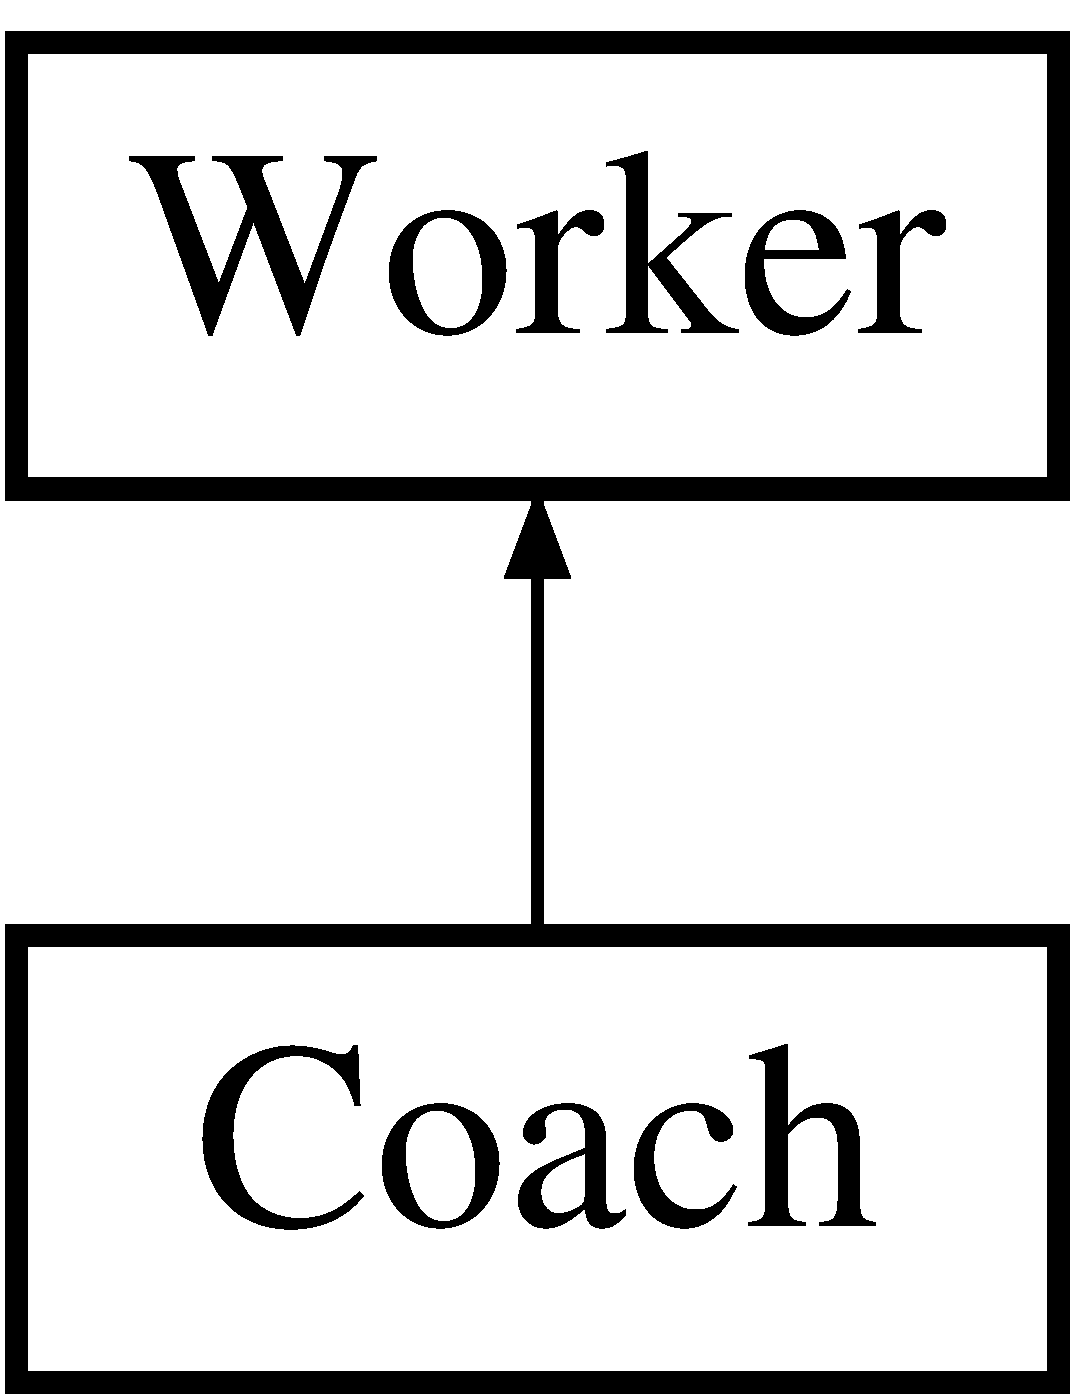
\includegraphics[height=2.000000cm]{class_coach}
\end{center}
\end{figure}
\subsection*{Public Member Functions}
\begin{DoxyCompactItemize}
\item 
\hyperlink{class_coach_af830e5ddd2f9e94118c98f953c0b2bde}{Coach} (string \hyperlink{class_worker_a66cf57341253a31e418cf8abad59ffb1}{name}, \hyperlink{class_date}{Date} \hyperlink{class_worker_a3c1845f40a084b471750a787a87614dd}{birthdate}, unsigned int \hyperlink{class_worker_adfafba55f967994f4595bd914bbba127}{civil\+ID}, \hyperlink{_utils_8hpp_ad6bce769911d709b802464c1ec12e7ad}{Coach\+Type} coach\+Role, unsigned int \hyperlink{class_worker_afc39287cd510977cfe7697ed2c86b2ca}{id}=0)
\begin{DoxyCompactList}\small\item\em \hyperlink{class_coach}{Coach} constructor. \end{DoxyCompactList}\item 
\hyperlink{class_coach_af578863f8d3846803ce9cccd280d6ffe}{Coach} (string \&new\+Coach)
\begin{DoxyCompactList}\small\item\em \hyperlink{class_coach}{Coach}\textquotesingle{}s Constructor that reads from the coaches\textquotesingle{} file. \end{DoxyCompactList}\item 
unsigned int \hyperlink{class_coach_a408361901fdbc11fd990b5fa26a94803}{get\+ID} () const
\begin{DoxyCompactList}\small\item\em Gets the coach\textquotesingle{}s identifier. \end{DoxyCompactList}\item 
bool \hyperlink{class_coach_a6329a96f3fea5b02b46b4e6caf519359}{is\+Athlete} () const
\begin{DoxyCompactList}\small\item\em Query if this object is athlete. \end{DoxyCompactList}\item 
unsigned int \hyperlink{class_coach_aa248ee0fec4a5dfdddb8c235ad4ae4a8}{get\+Position} () const
\begin{DoxyCompactList}\small\item\em Gets the coach\textquotesingle{}s position. \end{DoxyCompactList}\item 
unsigned int \hyperlink{class_coach_af899da3e98bc326b9abdf3ef46cf5279}{get\+Height} () const
\begin{DoxyCompactList}\small\item\em Gets the coach\textquotesingle{}s height. \end{DoxyCompactList}\item 
\hyperlink{class_info}{Info} $\ast$ \hyperlink{class_coach_a527d675556892403695d70c438d76151}{get\+Info} () const
\begin{DoxyCompactList}\small\item\em Gets the coach\textquotesingle{}s information. \end{DoxyCompactList}\item 
void \hyperlink{class_coach_a989f8c8ec5ba95849503f79376fc68bb}{add\+Info} (\hyperlink{class_info}{Info} $\ast$more\+Info)
\begin{DoxyCompactList}\small\item\em Adds an information. \end{DoxyCompactList}\item 
string \hyperlink{class_coach_a95f841d14e6994708a7f230a5d3a8d23}{generate\+Info} () const
\begin{DoxyCompactList}\small\item\em Generates the coach\textquotesingle{}s information. \end{DoxyCompactList}\item 
vector$<$ string $>$ \hyperlink{class_coach_a954ee94a35267f5992d1a84d25c15c7f}{show\+In\+Screen} () const
\begin{DoxyCompactList}\small\item\em Shows all the coach\textquotesingle{}s information in the screen. \end{DoxyCompactList}\item 
void \hyperlink{class_coach_aef508cef2680594ef837407790d00db6}{set\+Birth\+Date} (\hyperlink{class_date}{Date} new\+Birthdate)
\begin{DoxyCompactList}\small\item\em Sets the coach\textquotesingle{}s birth date. \end{DoxyCompactList}\item 
void \hyperlink{class_coach_a72de329d96f180eca4108c7103946ee3}{set\+Coach\+Type} (\hyperlink{_utils_8hpp_ad6bce769911d709b802464c1ec12e7ad}{Coach\+Type} new\+Type)
\begin{DoxyCompactList}\small\item\em Sets coach\textquotesingle{}s type. \end{DoxyCompactList}\end{DoxyCompactItemize}
\subsection*{Private Attributes}
\begin{DoxyCompactItemize}
\item 
\hyperlink{_utils_8hpp_ad6bce769911d709b802464c1ec12e7ad}{Coach\+Type} \hyperlink{class_coach_aac51e9d7398550135eb64a32e903002f}{trainer\+Position}
\begin{DoxyCompactList}\small\item\em coach\textquotesingle{}s position. \end{DoxyCompactList}\end{DoxyCompactItemize}
\subsection*{Additional Inherited Members}


\subsection{Detailed Description}
A coach. 

Lu�s, 20/11/2016. 

\subsection{Constructor \& Destructor Documentation}
\hypertarget{class_coach_af830e5ddd2f9e94118c98f953c0b2bde}{}\label{class_coach_af830e5ddd2f9e94118c98f953c0b2bde} 
\index{Coach@{Coach}!Coach@{Coach}}
\index{Coach@{Coach}!Coach@{Coach}}
\subsubsection{\texorpdfstring{Coach()}{Coach()}\hspace{0.1cm}{\footnotesize\ttfamily [1/2]}}
{\footnotesize\ttfamily Coach\+::\+Coach (\begin{DoxyParamCaption}\item[{string}]{name,  }\item[{\hyperlink{class_date}{Date}}]{birthdate,  }\item[{unsigned int}]{civil\+ID,  }\item[{\hyperlink{_utils_8hpp_ad6bce769911d709b802464c1ec12e7ad}{Coach\+Type}}]{coach\+Role,  }\item[{unsigned int}]{id = {\ttfamily 0} }\end{DoxyParamCaption})}



\hyperlink{class_coach}{Coach} constructor. 

This is a constructor that uses the name, birthdate, civil\+ID, coach\textquotesingle{}s role and id 

\hyperlink{class_coach}{Coach}\textquotesingle{}s Constructor. 

Lu�s, 20/11/2016. 


\begin{DoxyParams}{Parameters}
{\em name} & The name. \\
\hline
{\em birthdate} & The birthdate. \\
\hline
{\em civil\+ID} & Civil identifier. \\
\hline
{\em coach\+Role} & The coach role. \\
\hline
{\em id} & (Optional) The identifier. \\
\hline
\end{DoxyParams}
\hypertarget{class_coach_af578863f8d3846803ce9cccd280d6ffe}{}\label{class_coach_af578863f8d3846803ce9cccd280d6ffe} 
\index{Coach@{Coach}!Coach@{Coach}}
\index{Coach@{Coach}!Coach@{Coach}}
\subsubsection{\texorpdfstring{Coach()}{Coach()}\hspace{0.1cm}{\footnotesize\ttfamily [2/2]}}
{\footnotesize\ttfamily Coach\+::\+Coach (\begin{DoxyParamCaption}\item[{string \&}]{new\+Coach }\end{DoxyParamCaption})}



\hyperlink{class_coach}{Coach}\textquotesingle{}s Constructor that reads from the coaches\textquotesingle{} file. 

This is a constructor that uses the coach\textquotesingle{}s name

Lu�s, 20/11/2016. 


\begin{DoxyParams}{Parameters}
{\em new\+Coach} & \mbox{[}in,out\mbox{]} The new coach. \\
\hline
\end{DoxyParams}


\subsection{Member Function Documentation}
\hypertarget{class_coach_a989f8c8ec5ba95849503f79376fc68bb}{}\label{class_coach_a989f8c8ec5ba95849503f79376fc68bb} 
\index{Coach@{Coach}!add\+Info@{add\+Info}}
\index{add\+Info@{add\+Info}!Coach@{Coach}}
\subsubsection{\texorpdfstring{add\+Info()}{addInfo()}}
{\footnotesize\ttfamily void Coach\+::add\+Info (\begin{DoxyParamCaption}\item[{\hyperlink{class_info}{Info} $\ast$}]{more\+Info }\end{DoxyParamCaption})\hspace{0.3cm}{\ttfamily [inline]}, {\ttfamily [virtual]}}



Adds an information. 

Lu�s, 20/11/2016. 


\begin{DoxyParams}{Parameters}
{\em more\+Info} & If non-\/null, all the coach\textquotesingle{}s information. \\
\hline
\end{DoxyParams}


Reimplemented from \hyperlink{class_worker_ad54db262f7473cc729c371dd54e292eb}{Worker}.

\hypertarget{class_coach_a95f841d14e6994708a7f230a5d3a8d23}{}\label{class_coach_a95f841d14e6994708a7f230a5d3a8d23} 
\index{Coach@{Coach}!generate\+Info@{generate\+Info}}
\index{generate\+Info@{generate\+Info}!Coach@{Coach}}
\subsubsection{\texorpdfstring{generate\+Info()}{generateInfo()}}
{\footnotesize\ttfamily string Coach\+::generate\+Info (\begin{DoxyParamCaption}{ }\end{DoxyParamCaption}) const\hspace{0.3cm}{\ttfamily [virtual]}}



Generates the coach\textquotesingle{}s information. 

Lu�s, 20/11/2016. 

\begin{DoxyReturn}{Returns}
The coach\textquotesingle{}s information. 
\end{DoxyReturn}


Reimplemented from \hyperlink{class_worker_ac77905603b86c58cb0a87d6389dca744}{Worker}.

\hypertarget{class_coach_af899da3e98bc326b9abdf3ef46cf5279}{}\label{class_coach_af899da3e98bc326b9abdf3ef46cf5279} 
\index{Coach@{Coach}!get\+Height@{get\+Height}}
\index{get\+Height@{get\+Height}!Coach@{Coach}}
\subsubsection{\texorpdfstring{get\+Height()}{getHeight()}}
{\footnotesize\ttfamily unsigned int Coach\+::get\+Height (\begin{DoxyParamCaption}{ }\end{DoxyParamCaption}) const\hspace{0.3cm}{\ttfamily [virtual]}}



Gets the coach\textquotesingle{}s height. 

Lu�s, 20/11/2016. 

\begin{DoxyReturn}{Returns}
The coach\textquotesingle{}s height. 
\end{DoxyReturn}


Implements \hyperlink{class_worker_a1c5dcdc1c7dc5e498a44f678e964bbfd}{Worker}.

\hypertarget{class_coach_a408361901fdbc11fd990b5fa26a94803}{}\label{class_coach_a408361901fdbc11fd990b5fa26a94803} 
\index{Coach@{Coach}!get\+ID@{get\+ID}}
\index{get\+ID@{get\+ID}!Coach@{Coach}}
\subsubsection{\texorpdfstring{get\+I\+D()}{getID()}}
{\footnotesize\ttfamily unsigned int Coach\+::get\+ID (\begin{DoxyParamCaption}{ }\end{DoxyParamCaption}) const\hspace{0.3cm}{\ttfamily [virtual]}}



Gets the coach\textquotesingle{}s identifier. 

Lu�s, 20/11/2016. 

\begin{DoxyReturn}{Returns}
The coach\textquotesingle{}s identifier. 
\end{DoxyReturn}


Implements \hyperlink{class_worker_a8b3e221c4a1ebd12ade03ee9b9c86182}{Worker}.

\hypertarget{class_coach_a527d675556892403695d70c438d76151}{}\label{class_coach_a527d675556892403695d70c438d76151} 
\index{Coach@{Coach}!get\+Info@{get\+Info}}
\index{get\+Info@{get\+Info}!Coach@{Coach}}
\subsubsection{\texorpdfstring{get\+Info()}{getInfo()}}
{\footnotesize\ttfamily \hyperlink{class_info}{Info}$\ast$ Coach\+::get\+Info (\begin{DoxyParamCaption}{ }\end{DoxyParamCaption}) const\hspace{0.3cm}{\ttfamily [inline]}, {\ttfamily [virtual]}}



Gets the coach\textquotesingle{}s information. 

This is a method that gets the coach\textquotesingle{}s information

Lu�s, 20/11/2016. 

\begin{DoxyReturn}{Returns}
Null if it fails, else the coach\textquotesingle{}s information. 
\end{DoxyReturn}


Reimplemented from \hyperlink{class_worker_a95a4f7c750644937859b8e14515a480e}{Worker}.

\hypertarget{class_coach_aa248ee0fec4a5dfdddb8c235ad4ae4a8}{}\label{class_coach_aa248ee0fec4a5dfdddb8c235ad4ae4a8} 
\index{Coach@{Coach}!get\+Position@{get\+Position}}
\index{get\+Position@{get\+Position}!Coach@{Coach}}
\subsubsection{\texorpdfstring{get\+Position()}{getPosition()}}
{\footnotesize\ttfamily unsigned int Coach\+::get\+Position (\begin{DoxyParamCaption}{ }\end{DoxyParamCaption}) const\hspace{0.3cm}{\ttfamily [virtual]}}



Gets the coach\textquotesingle{}s position. 

This is a method that gets the coach\textquotesingle{}s position

Lu�s, 20/11/2016. 

\begin{DoxyReturn}{Returns}
The coah\textquotesingle{}s position. 
\end{DoxyReturn}


Implements \hyperlink{class_worker_a5fd37dea8c5e6579c1deecbfc1b22db9}{Worker}.

\hypertarget{class_coach_a6329a96f3fea5b02b46b4e6caf519359}{}\label{class_coach_a6329a96f3fea5b02b46b4e6caf519359} 
\index{Coach@{Coach}!is\+Athlete@{is\+Athlete}}
\index{is\+Athlete@{is\+Athlete}!Coach@{Coach}}
\subsubsection{\texorpdfstring{is\+Athlete()}{isAthlete()}}
{\footnotesize\ttfamily bool Coach\+::is\+Athlete (\begin{DoxyParamCaption}{ }\end{DoxyParamCaption}) const\hspace{0.3cm}{\ttfamily [virtual]}}



Query if this object is athlete. 

This is a method that checks if the worker is an athlete

Lu�s, 20/11/2016. 

\begin{DoxyReturn}{Returns}
True if athlete, false if not. 
\end{DoxyReturn}


Implements \hyperlink{class_worker_a0a2eb7505b3a734184be3dfdf3316cc3}{Worker}.

\hypertarget{class_coach_aef508cef2680594ef837407790d00db6}{}\label{class_coach_aef508cef2680594ef837407790d00db6} 
\index{Coach@{Coach}!set\+Birth\+Date@{set\+Birth\+Date}}
\index{set\+Birth\+Date@{set\+Birth\+Date}!Coach@{Coach}}
\subsubsection{\texorpdfstring{set\+Birth\+Date()}{setBirthDate()}}
{\footnotesize\ttfamily void Coach\+::set\+Birth\+Date (\begin{DoxyParamCaption}\item[{\hyperlink{class_date}{Date}}]{new\+Birthdate }\end{DoxyParamCaption})\hspace{0.3cm}{\ttfamily [virtual]}}



Sets the coach\textquotesingle{}s birth date. 

Lu�s, 20/11/2016. 


\begin{DoxyParams}{Parameters}
{\em new\+Birthdate} & The new birthdate. \\
\hline
\end{DoxyParams}


Reimplemented from \hyperlink{class_worker_ac48a8315ccdeb2913cd98ea223660f72}{Worker}.

\hypertarget{class_coach_a72de329d96f180eca4108c7103946ee3}{}\label{class_coach_a72de329d96f180eca4108c7103946ee3} 
\index{Coach@{Coach}!set\+Coach\+Type@{set\+Coach\+Type}}
\index{set\+Coach\+Type@{set\+Coach\+Type}!Coach@{Coach}}
\subsubsection{\texorpdfstring{set\+Coach\+Type()}{setCoachType()}}
{\footnotesize\ttfamily void Coach\+::set\+Coach\+Type (\begin{DoxyParamCaption}\item[{\hyperlink{_utils_8hpp_ad6bce769911d709b802464c1ec12e7ad}{Coach\+Type}}]{new\+Type }\end{DoxyParamCaption})\hspace{0.3cm}{\ttfamily [virtual]}}



Sets coach\textquotesingle{}s type. 

Lu�s, 20/11/2016. 


\begin{DoxyParams}{Parameters}
{\em new\+Type} & New coach\textquotesingle{}s type. \\
\hline
\end{DoxyParams}


Reimplemented from \hyperlink{class_worker_ae84b05468a6fdbadad9163bfc18e0569}{Worker}.

\hypertarget{class_coach_a954ee94a35267f5992d1a84d25c15c7f}{}\label{class_coach_a954ee94a35267f5992d1a84d25c15c7f} 
\index{Coach@{Coach}!show\+In\+Screen@{show\+In\+Screen}}
\index{show\+In\+Screen@{show\+In\+Screen}!Coach@{Coach}}
\subsubsection{\texorpdfstring{show\+In\+Screen()}{showInScreen()}}
{\footnotesize\ttfamily vector$<$ string $>$ Coach\+::show\+In\+Screen (\begin{DoxyParamCaption}{ }\end{DoxyParamCaption}) const\hspace{0.3cm}{\ttfamily [virtual]}}



Shows all the coach\textquotesingle{}s information in the screen. 

Lu�s, 20/11/2016. 

\begin{DoxyReturn}{Returns}
A vector of strings; 
\end{DoxyReturn}


Reimplemented from \hyperlink{class_worker_aca1475c72f6e7c6b85114b0bba0da038}{Worker}.



\subsection{Member Data Documentation}
\hypertarget{class_coach_aac51e9d7398550135eb64a32e903002f}{}\label{class_coach_aac51e9d7398550135eb64a32e903002f} 
\index{Coach@{Coach}!trainer\+Position@{trainer\+Position}}
\index{trainer\+Position@{trainer\+Position}!Coach@{Coach}}
\subsubsection{\texorpdfstring{trainer\+Position}{trainerPosition}}
{\footnotesize\ttfamily \hyperlink{_utils_8hpp_ad6bce769911d709b802464c1ec12e7ad}{Coach\+Type} Coach\+::trainer\+Position\hspace{0.3cm}{\ttfamily [private]}}



coach\textquotesingle{}s position. 



The documentation for this class was generated from the following files\+:\begin{DoxyCompactItemize}
\item 
\hyperlink{_coach_8hpp}{Coach.\+hpp}\item 
\hyperlink{_coach_8cpp}{Coach.\+cpp}\end{DoxyCompactItemize}

\hypertarget{class_date}{}\section{Date Class Reference}
\label{class_date}\index{Date@{Date}}


{\ttfamily \#include $<$Utils.\+hpp$>$}

\subsection*{Public Member Functions}
\begin{DoxyCompactItemize}
\item 
\hyperlink{class_date_a4e59ed4ba66eec61c27460c5d09fa1bd}{Date} ()
\item 
\hyperlink{class_date_aed0ec4ac9e00fb6130f8a642a61180b9}{Date} (string data)
\item 
\hyperlink{class_date_ae0f1f3db515c009b0a9f77869edc7599}{Date} (unsigned int dia, unsigned int mes, unsigned int ano)
\item 
\hyperlink{class_date_a5b859c0abe4bcf936dc7a7124e079659}{Date} (ifstream \&in\+Stream)
\item 
int \hyperlink{class_date_a0f253815240e70f4c39cb93cc68bd3f4}{get\+Day} () const
\item 
int \hyperlink{class_date_a332f6e3a2f6a40d73742b6dab7be0f64}{get\+Month} () const
\item 
int \hyperlink{class_date_a8b0869f34c2b38d108ab83ee2e770e5d}{get\+Year} () const
\item 
void \hyperlink{class_date_a742b1032af5bbd3e4c9ddfc9c21c1a5a}{set\+Day} (int dia)
\item 
void \hyperlink{class_date_a11b56160e1dbb550b68a7dd54c968204}{set\+Month} (int mes)
\item 
void \hyperlink{class_date_a62230a93ff2ce92cd4b30408622393af}{set\+Year} (int ano)
\item 
void \hyperlink{class_date_af7ea8f12ad1c018f58dbc85f9c844b03}{save} (ofstream \&out) const
\item 
string \hyperlink{class_date_affb645fa983d4e0317ba0aa8f5998fd1}{show\+Date} () const
\item 
void \hyperlink{class_date_ada293ae20419963c246a7831096f6091}{set\+Current\+Date} ()
\item 
string \hyperlink{class_date_a5ea4980f43e2b098e033651e199d2793}{str} () const
\end{DoxyCompactItemize}
\subsection*{Private Member Functions}
\begin{DoxyCompactItemize}
\item 
bool \hyperlink{class_date_a434957869afa4b4e1275e00fe6a67216}{is\+Leap} (int \hyperlink{class_date_a3eeced2ed56bc95d56782b9e738db8ea}{year}) const
\item 
int \hyperlink{class_date_a102f0523e4d84ad9cef682f2ff233808}{num\+Days} (int \hyperlink{class_date_a533843e07c6ac8d19fee9b16f5336ba2}{month}, int \hyperlink{class_date_a3eeced2ed56bc95d56782b9e738db8ea}{year}) const
\end{DoxyCompactItemize}
\subsection*{Private Attributes}
\begin{DoxyCompactItemize}
\item 
int \hyperlink{class_date_a5b192adcabf2b2871e3f0b76c1ec1601}{day}
\item 
int \hyperlink{class_date_a533843e07c6ac8d19fee9b16f5336ba2}{month}
\item 
int \hyperlink{class_date_a3eeced2ed56bc95d56782b9e738db8ea}{year}
\end{DoxyCompactItemize}
\subsection*{Friends}
\begin{DoxyCompactItemize}
\item 
ifstream \& \hyperlink{class_date_ab895bef0d8545ab4875f6bfc4a7fd4f7}{operator$>$$>$} (ifstream \&in\+Stream, \hyperlink{class_date}{Date} \&date\+To\+Read)
\item 
bool \hyperlink{class_date_ad9736995fa90a35631dc5f220e33e4b2}{operator$>$=} (const \hyperlink{class_date}{Date} \&date1, const \hyperlink{class_date}{Date} date2)
\item 
bool \hyperlink{class_date_aa2e695ccf211714fafbc8c73cb7e5419}{operator$<$} (const \hyperlink{class_date}{Date} \&date1, const \hyperlink{class_date}{Date} \&date2)
\item 
bool \hyperlink{class_date_a588c6068972f9e69bc50292405c1fac7}{operator==} (const \hyperlink{class_date}{Date} \&date1, const \hyperlink{class_date}{Date} \&date2)
\item 
ostream \& \hyperlink{class_date_a7f6a6b50c5a5aca26dd5b5631c2f5c43}{operator$<$$<$} (ostream \&out, const \hyperlink{class_date}{Date} \&data)
\item 
int \hyperlink{class_date_ac5bf05534baacb5dc11f6abbb4e1f621}{operator-\/} (const \hyperlink{class_date}{Date} \&date1, const \hyperlink{class_date}{Date} \&date2)
\end{DoxyCompactItemize}


\subsection{Constructor \& Destructor Documentation}
\hypertarget{class_date_a4e59ed4ba66eec61c27460c5d09fa1bd}{}\label{class_date_a4e59ed4ba66eec61c27460c5d09fa1bd} 
\index{Date@{Date}!Date@{Date}}
\index{Date@{Date}!Date@{Date}}
\subsubsection{\texorpdfstring{Date()}{Date()}\hspace{0.1cm}{\footnotesize\ttfamily [1/4]}}
{\footnotesize\ttfamily Date\+::\+Date (\begin{DoxyParamCaption}{ }\end{DoxyParamCaption})}

\hypertarget{class_date_aed0ec4ac9e00fb6130f8a642a61180b9}{}\label{class_date_aed0ec4ac9e00fb6130f8a642a61180b9} 
\index{Date@{Date}!Date@{Date}}
\index{Date@{Date}!Date@{Date}}
\subsubsection{\texorpdfstring{Date()}{Date()}\hspace{0.1cm}{\footnotesize\ttfamily [2/4]}}
{\footnotesize\ttfamily Date\+::\+Date (\begin{DoxyParamCaption}\item[{string}]{data }\end{DoxyParamCaption})}

\hypertarget{class_date_ae0f1f3db515c009b0a9f77869edc7599}{}\label{class_date_ae0f1f3db515c009b0a9f77869edc7599} 
\index{Date@{Date}!Date@{Date}}
\index{Date@{Date}!Date@{Date}}
\subsubsection{\texorpdfstring{Date()}{Date()}\hspace{0.1cm}{\footnotesize\ttfamily [3/4]}}
{\footnotesize\ttfamily Date\+::\+Date (\begin{DoxyParamCaption}\item[{unsigned int}]{dia,  }\item[{unsigned int}]{mes,  }\item[{unsigned int}]{ano }\end{DoxyParamCaption})}

\hypertarget{class_date_a5b859c0abe4bcf936dc7a7124e079659}{}\label{class_date_a5b859c0abe4bcf936dc7a7124e079659} 
\index{Date@{Date}!Date@{Date}}
\index{Date@{Date}!Date@{Date}}
\subsubsection{\texorpdfstring{Date()}{Date()}\hspace{0.1cm}{\footnotesize\ttfamily [4/4]}}
{\footnotesize\ttfamily Date\+::\+Date (\begin{DoxyParamCaption}\item[{ifstream \&}]{in\+Stream }\end{DoxyParamCaption})}



\subsection{Member Function Documentation}
\hypertarget{class_date_a0f253815240e70f4c39cb93cc68bd3f4}{}\label{class_date_a0f253815240e70f4c39cb93cc68bd3f4} 
\index{Date@{Date}!get\+Day@{get\+Day}}
\index{get\+Day@{get\+Day}!Date@{Date}}
\subsubsection{\texorpdfstring{get\+Day()}{getDay()}}
{\footnotesize\ttfamily int Date\+::get\+Day (\begin{DoxyParamCaption}{ }\end{DoxyParamCaption}) const}

\hypertarget{class_date_a332f6e3a2f6a40d73742b6dab7be0f64}{}\label{class_date_a332f6e3a2f6a40d73742b6dab7be0f64} 
\index{Date@{Date}!get\+Month@{get\+Month}}
\index{get\+Month@{get\+Month}!Date@{Date}}
\subsubsection{\texorpdfstring{get\+Month()}{getMonth()}}
{\footnotesize\ttfamily int Date\+::get\+Month (\begin{DoxyParamCaption}{ }\end{DoxyParamCaption}) const}

\hypertarget{class_date_a8b0869f34c2b38d108ab83ee2e770e5d}{}\label{class_date_a8b0869f34c2b38d108ab83ee2e770e5d} 
\index{Date@{Date}!get\+Year@{get\+Year}}
\index{get\+Year@{get\+Year}!Date@{Date}}
\subsubsection{\texorpdfstring{get\+Year()}{getYear()}}
{\footnotesize\ttfamily int Date\+::get\+Year (\begin{DoxyParamCaption}{ }\end{DoxyParamCaption}) const}

\hypertarget{class_date_a434957869afa4b4e1275e00fe6a67216}{}\label{class_date_a434957869afa4b4e1275e00fe6a67216} 
\index{Date@{Date}!is\+Leap@{is\+Leap}}
\index{is\+Leap@{is\+Leap}!Date@{Date}}
\subsubsection{\texorpdfstring{is\+Leap()}{isLeap()}}
{\footnotesize\ttfamily bool Date\+::is\+Leap (\begin{DoxyParamCaption}\item[{int}]{year }\end{DoxyParamCaption}) const\hspace{0.3cm}{\ttfamily [private]}}

\hypertarget{class_date_a102f0523e4d84ad9cef682f2ff233808}{}\label{class_date_a102f0523e4d84ad9cef682f2ff233808} 
\index{Date@{Date}!num\+Days@{num\+Days}}
\index{num\+Days@{num\+Days}!Date@{Date}}
\subsubsection{\texorpdfstring{num\+Days()}{numDays()}}
{\footnotesize\ttfamily int Date\+::num\+Days (\begin{DoxyParamCaption}\item[{int}]{month,  }\item[{int}]{year }\end{DoxyParamCaption}) const\hspace{0.3cm}{\ttfamily [private]}}

\hypertarget{class_date_af7ea8f12ad1c018f58dbc85f9c844b03}{}\label{class_date_af7ea8f12ad1c018f58dbc85f9c844b03} 
\index{Date@{Date}!save@{save}}
\index{save@{save}!Date@{Date}}
\subsubsection{\texorpdfstring{save()}{save()}}
{\footnotesize\ttfamily void Date\+::save (\begin{DoxyParamCaption}\item[{ofstream \&}]{out }\end{DoxyParamCaption}) const}

\hypertarget{class_date_ada293ae20419963c246a7831096f6091}{}\label{class_date_ada293ae20419963c246a7831096f6091} 
\index{Date@{Date}!set\+Current\+Date@{set\+Current\+Date}}
\index{set\+Current\+Date@{set\+Current\+Date}!Date@{Date}}
\subsubsection{\texorpdfstring{set\+Current\+Date()}{setCurrentDate()}}
{\footnotesize\ttfamily void Date\+::set\+Current\+Date (\begin{DoxyParamCaption}{ }\end{DoxyParamCaption})}

\hypertarget{class_date_a742b1032af5bbd3e4c9ddfc9c21c1a5a}{}\label{class_date_a742b1032af5bbd3e4c9ddfc9c21c1a5a} 
\index{Date@{Date}!set\+Day@{set\+Day}}
\index{set\+Day@{set\+Day}!Date@{Date}}
\subsubsection{\texorpdfstring{set\+Day()}{setDay()}}
{\footnotesize\ttfamily void Date\+::set\+Day (\begin{DoxyParamCaption}\item[{int}]{dia }\end{DoxyParamCaption})}

\hypertarget{class_date_a11b56160e1dbb550b68a7dd54c968204}{}\label{class_date_a11b56160e1dbb550b68a7dd54c968204} 
\index{Date@{Date}!set\+Month@{set\+Month}}
\index{set\+Month@{set\+Month}!Date@{Date}}
\subsubsection{\texorpdfstring{set\+Month()}{setMonth()}}
{\footnotesize\ttfamily void Date\+::set\+Month (\begin{DoxyParamCaption}\item[{int}]{mes }\end{DoxyParamCaption})}

\hypertarget{class_date_a62230a93ff2ce92cd4b30408622393af}{}\label{class_date_a62230a93ff2ce92cd4b30408622393af} 
\index{Date@{Date}!set\+Year@{set\+Year}}
\index{set\+Year@{set\+Year}!Date@{Date}}
\subsubsection{\texorpdfstring{set\+Year()}{setYear()}}
{\footnotesize\ttfamily void Date\+::set\+Year (\begin{DoxyParamCaption}\item[{int}]{ano }\end{DoxyParamCaption})}

\hypertarget{class_date_affb645fa983d4e0317ba0aa8f5998fd1}{}\label{class_date_affb645fa983d4e0317ba0aa8f5998fd1} 
\index{Date@{Date}!show\+Date@{show\+Date}}
\index{show\+Date@{show\+Date}!Date@{Date}}
\subsubsection{\texorpdfstring{show\+Date()}{showDate()}}
{\footnotesize\ttfamily string Date\+::show\+Date (\begin{DoxyParamCaption}{ }\end{DoxyParamCaption}) const}

\hypertarget{class_date_a5ea4980f43e2b098e033651e199d2793}{}\label{class_date_a5ea4980f43e2b098e033651e199d2793} 
\index{Date@{Date}!str@{str}}
\index{str@{str}!Date@{Date}}
\subsubsection{\texorpdfstring{str()}{str()}}
{\footnotesize\ttfamily string Date\+::str (\begin{DoxyParamCaption}{ }\end{DoxyParamCaption}) const}



\subsection{Friends And Related Function Documentation}
\hypertarget{class_date_ac5bf05534baacb5dc11f6abbb4e1f621}{}\label{class_date_ac5bf05534baacb5dc11f6abbb4e1f621} 
\index{Date@{Date}!operator-\/@{operator-\/}}
\index{operator-\/@{operator-\/}!Date@{Date}}
\subsubsection{\texorpdfstring{operator-\/}{operator-}}
{\footnotesize\ttfamily int operator-\/ (\begin{DoxyParamCaption}\item[{const \hyperlink{class_date}{Date} \&}]{date1,  }\item[{const \hyperlink{class_date}{Date} \&}]{date2 }\end{DoxyParamCaption})\hspace{0.3cm}{\ttfamily [friend]}}

\hypertarget{class_date_aa2e695ccf211714fafbc8c73cb7e5419}{}\label{class_date_aa2e695ccf211714fafbc8c73cb7e5419} 
\index{Date@{Date}!operator$<$@{operator$<$}}
\index{operator$<$@{operator$<$}!Date@{Date}}
\subsubsection{\texorpdfstring{operator$<$}{operator<}}
{\footnotesize\ttfamily bool operator$<$ (\begin{DoxyParamCaption}\item[{const \hyperlink{class_date}{Date} \&}]{date1,  }\item[{const \hyperlink{class_date}{Date} \&}]{date2 }\end{DoxyParamCaption})\hspace{0.3cm}{\ttfamily [friend]}}

\hypertarget{class_date_a7f6a6b50c5a5aca26dd5b5631c2f5c43}{}\label{class_date_a7f6a6b50c5a5aca26dd5b5631c2f5c43} 
\index{Date@{Date}!operator$<$$<$@{operator$<$$<$}}
\index{operator$<$$<$@{operator$<$$<$}!Date@{Date}}
\subsubsection{\texorpdfstring{operator$<$$<$}{operator<<}}
{\footnotesize\ttfamily ostream\& operator$<$$<$ (\begin{DoxyParamCaption}\item[{ostream \&}]{out,  }\item[{const \hyperlink{class_date}{Date} \&}]{data }\end{DoxyParamCaption})\hspace{0.3cm}{\ttfamily [friend]}}

\hypertarget{class_date_a588c6068972f9e69bc50292405c1fac7}{}\label{class_date_a588c6068972f9e69bc50292405c1fac7} 
\index{Date@{Date}!operator==@{operator==}}
\index{operator==@{operator==}!Date@{Date}}
\subsubsection{\texorpdfstring{operator==}{operator==}}
{\footnotesize\ttfamily bool operator== (\begin{DoxyParamCaption}\item[{const \hyperlink{class_date}{Date} \&}]{date1,  }\item[{const \hyperlink{class_date}{Date} \&}]{date2 }\end{DoxyParamCaption})\hspace{0.3cm}{\ttfamily [friend]}}

\hypertarget{class_date_ad9736995fa90a35631dc5f220e33e4b2}{}\label{class_date_ad9736995fa90a35631dc5f220e33e4b2} 
\index{Date@{Date}!operator$>$=@{operator$>$=}}
\index{operator$>$=@{operator$>$=}!Date@{Date}}
\subsubsection{\texorpdfstring{operator$>$=}{operator>=}}
{\footnotesize\ttfamily bool operator$>$= (\begin{DoxyParamCaption}\item[{const \hyperlink{class_date}{Date} \&}]{date1,  }\item[{const \hyperlink{class_date}{Date}}]{date2 }\end{DoxyParamCaption})\hspace{0.3cm}{\ttfamily [friend]}}

\hypertarget{class_date_ab895bef0d8545ab4875f6bfc4a7fd4f7}{}\label{class_date_ab895bef0d8545ab4875f6bfc4a7fd4f7} 
\index{Date@{Date}!operator$>$$>$@{operator$>$$>$}}
\index{operator$>$$>$@{operator$>$$>$}!Date@{Date}}
\subsubsection{\texorpdfstring{operator$>$$>$}{operator>>}}
{\footnotesize\ttfamily ifstream\& operator$>$$>$ (\begin{DoxyParamCaption}\item[{ifstream \&}]{in\+Stream,  }\item[{\hyperlink{class_date}{Date} \&}]{date\+To\+Read }\end{DoxyParamCaption})\hspace{0.3cm}{\ttfamily [friend]}}



\subsection{Member Data Documentation}
\hypertarget{class_date_a5b192adcabf2b2871e3f0b76c1ec1601}{}\label{class_date_a5b192adcabf2b2871e3f0b76c1ec1601} 
\index{Date@{Date}!day@{day}}
\index{day@{day}!Date@{Date}}
\subsubsection{\texorpdfstring{day}{day}}
{\footnotesize\ttfamily int Date\+::day\hspace{0.3cm}{\ttfamily [private]}}

\hypertarget{class_date_a533843e07c6ac8d19fee9b16f5336ba2}{}\label{class_date_a533843e07c6ac8d19fee9b16f5336ba2} 
\index{Date@{Date}!month@{month}}
\index{month@{month}!Date@{Date}}
\subsubsection{\texorpdfstring{month}{month}}
{\footnotesize\ttfamily int Date\+::month\hspace{0.3cm}{\ttfamily [private]}}

\hypertarget{class_date_a3eeced2ed56bc95d56782b9e738db8ea}{}\label{class_date_a3eeced2ed56bc95d56782b9e738db8ea} 
\index{Date@{Date}!year@{year}}
\index{year@{year}!Date@{Date}}
\subsubsection{\texorpdfstring{year}{year}}
{\footnotesize\ttfamily int Date\+::year\hspace{0.3cm}{\ttfamily [private]}}



The documentation for this class was generated from the following files\+:\begin{DoxyCompactItemize}
\item 
\hyperlink{_utils_8hpp}{Utils.\+hpp}\item 
\hyperlink{_utils_8cpp}{Utils.\+cpp}\end{DoxyCompactItemize}

\hypertarget{class_defender}{}\section{Defender Class Reference}
\label{class_defender}\index{Defender@{Defender}}


A defender.  




{\ttfamily \#include $<$Defender.\+hpp$>$}

Inheritance diagram for Defender\+:\begin{figure}[H]
\begin{center}
\leavevmode
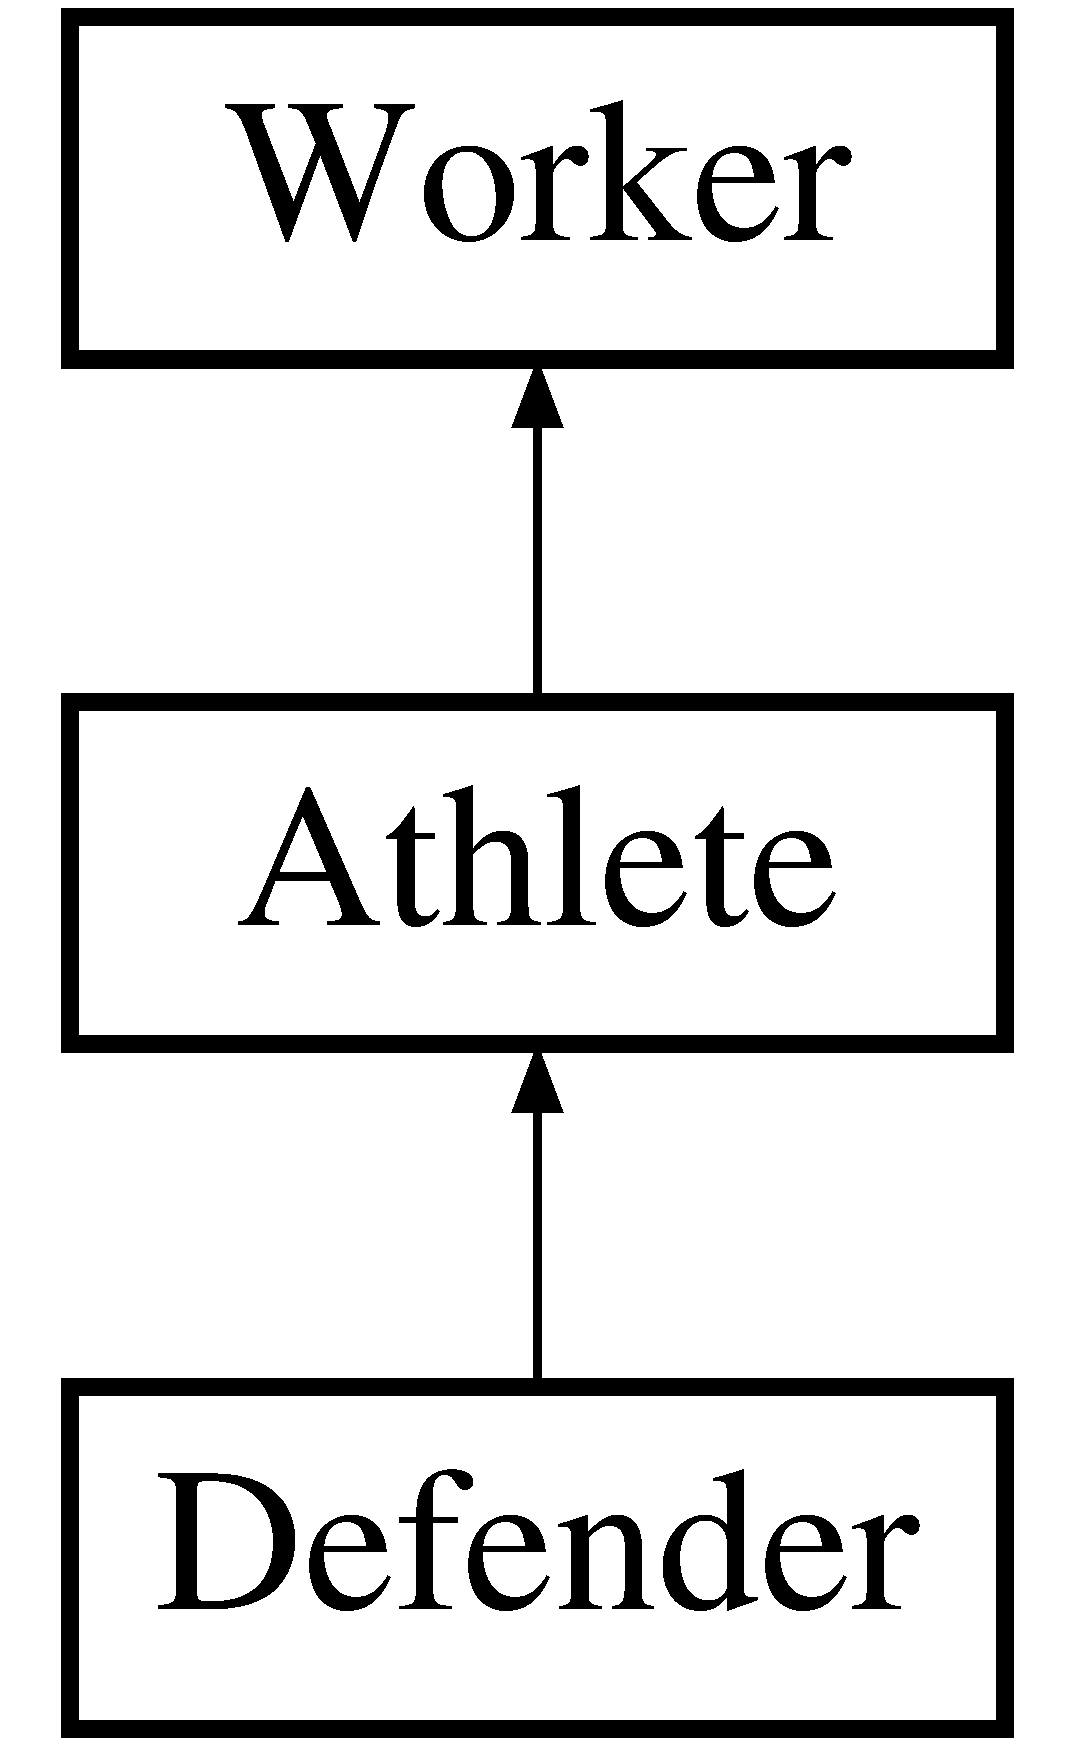
\includegraphics[height=3.000000cm]{class_defender}
\end{center}
\end{figure}
\subsection*{Public Member Functions}
\begin{DoxyCompactItemize}
\item 
\hyperlink{class_defender_aa09b1f02e3314aef1463528b3a0c70e2}{Defender} (string \hyperlink{class_worker_a66cf57341253a31e418cf8abad59ffb1}{name}, \hyperlink{class_date}{Date} \hyperlink{class_worker_a3c1845f40a084b471750a787a87614dd}{birthdate}, unsigned int \hyperlink{class_worker_adfafba55f967994f4595bd914bbba127}{civil\+ID}, unsigned char \hyperlink{class_athlete_a80a64bb1d5c943aaa7ca152d596d9914}{height}, unsigned int=0)
\begin{DoxyCompactList}\small\item\em Constructor. The id is set automatically \end{DoxyCompactList}\item 
\hyperlink{class_defender_a2ad862369c0babb9fc303d43bfa3321b}{Defender} (string \&new\+DF)
\begin{DoxyCompactList}\small\item\em Constructor that reads from the athlete\textquotesingle{}s file. \end{DoxyCompactList}\item 
\hyperlink{class_defender_ac0872f9e6cae6078b87cbcf9fa32f3ba}{$\sim$\+Defender} ()
\begin{DoxyCompactList}\small\item\em Destructor. \end{DoxyCompactList}\item 
unsigned int \hyperlink{class_defender_ad2aadb1cb382bf08522bd858ecc69667}{get\+ID} () const
\begin{DoxyCompactList}\small\item\em Gets the defender\textquotesingle{}s identifier. \end{DoxyCompactList}\item 
\hyperlink{class_info}{Info} $\ast$ \hyperlink{class_defender_a54de21eac6353f8847ac109b8a08fcab}{get\+Info} () const
\begin{DoxyCompactList}\small\item\em Gets the defender\textquotesingle{}s performance information. \end{DoxyCompactList}\item 
void \hyperlink{class_defender_abcd887808491719d6e40d92d68862b4e}{add\+Info} (\hyperlink{class_info}{Info} $\ast$more\+Info)
\begin{DoxyCompactList}\small\item\em Adds information to the defender. \end{DoxyCompactList}\end{DoxyCompactItemize}
\subsection*{Private Attributes}
\begin{DoxyCompactItemize}
\item 
\hyperlink{class_info}{Info} $\ast$ \hyperlink{class_defender_a849c8836a0dff2abd8df7a8d6434cc8c}{general\+Info}
\begin{DoxyCompactList}\small\item\em defender\textquotesingle{}s general info. \end{DoxyCompactList}\end{DoxyCompactItemize}
\subsection*{Additional Inherited Members}


\subsection{Detailed Description}
A defender. 

Luís, 20/11/2016. 

\subsection{Constructor \& Destructor Documentation}
\hypertarget{class_defender_aa09b1f02e3314aef1463528b3a0c70e2}{}\label{class_defender_aa09b1f02e3314aef1463528b3a0c70e2} 
\index{Defender@{Defender}!Defender@{Defender}}
\index{Defender@{Defender}!Defender@{Defender}}
\subsubsection{\texorpdfstring{Defender()}{Defender()}\hspace{0.1cm}{\footnotesize\ttfamily [1/2]}}
{\footnotesize\ttfamily Defender\+::\+Defender (\begin{DoxyParamCaption}\item[{string}]{name,  }\item[{\hyperlink{class_date}{Date}}]{birthdate,  }\item[{unsigned int}]{civil\+ID,  }\item[{unsigned char}]{height,  }\item[{unsigned int}]{id = {\ttfamily 0} }\end{DoxyParamCaption})}



Constructor. The id is set automatically 

Luís, 20/11/2016. 


\begin{DoxyParams}{Parameters}
{\em name} & The name. \\
\hline
{\em birthdate} & The birthdate. \\
\hline
{\em civil\+ID} & Civil identifier. \\
\hline
{\em height} & The height. \\
\hline
\end{DoxyParams}
\hypertarget{class_defender_a2ad862369c0babb9fc303d43bfa3321b}{}\label{class_defender_a2ad862369c0babb9fc303d43bfa3321b} 
\index{Defender@{Defender}!Defender@{Defender}}
\index{Defender@{Defender}!Defender@{Defender}}
\subsubsection{\texorpdfstring{Defender()}{Defender()}\hspace{0.1cm}{\footnotesize\ttfamily [2/2]}}
{\footnotesize\ttfamily Defender\+::\+Defender (\begin{DoxyParamCaption}\item[{string \&}]{new\+DF }\end{DoxyParamCaption})}



Constructor that reads from the athlete\textquotesingle{}s file. 

Luís, 20/11/2016. 


\begin{DoxyParams}{Parameters}
{\em new\+DF} & \mbox{[}in,out\mbox{]} The new df. \\
\hline
\end{DoxyParams}
\hypertarget{class_defender_ac0872f9e6cae6078b87cbcf9fa32f3ba}{}\label{class_defender_ac0872f9e6cae6078b87cbcf9fa32f3ba} 
\index{Defender@{Defender}!````~Defender@{$\sim$\+Defender}}
\index{````~Defender@{$\sim$\+Defender}!Defender@{Defender}}
\subsubsection{\texorpdfstring{$\sim$\+Defender()}{~Defender()}}
{\footnotesize\ttfamily Defender\+::$\sim$\+Defender (\begin{DoxyParamCaption}{ }\end{DoxyParamCaption})}



Destructor. 

Luís, 20/11/2016. 

\subsection{Member Function Documentation}
\hypertarget{class_defender_abcd887808491719d6e40d92d68862b4e}{}\label{class_defender_abcd887808491719d6e40d92d68862b4e} 
\index{Defender@{Defender}!add\+Info@{add\+Info}}
\index{add\+Info@{add\+Info}!Defender@{Defender}}
\subsubsection{\texorpdfstring{add\+Info()}{addInfo()}}
{\footnotesize\ttfamily void Defender\+::add\+Info (\begin{DoxyParamCaption}\item[{\hyperlink{class_info}{Info} $\ast$}]{more\+Info }\end{DoxyParamCaption})\hspace{0.3cm}{\ttfamily [virtual]}}



Adds information to the defender. 

Luís, 20/11/2016. 


\begin{DoxyParams}{Parameters}
{\em more\+Info} & \mbox{[}in,out\mbox{]} If non-\/null, all the defender\textquotesingle{}s performance information. \\
\hline
\end{DoxyParams}


Reimplemented from \hyperlink{class_worker_ad54db262f7473cc729c371dd54e292eb}{Worker}.

\hypertarget{class_defender_ad2aadb1cb382bf08522bd858ecc69667}{}\label{class_defender_ad2aadb1cb382bf08522bd858ecc69667} 
\index{Defender@{Defender}!get\+ID@{get\+ID}}
\index{get\+ID@{get\+ID}!Defender@{Defender}}
\subsubsection{\texorpdfstring{get\+I\+D()}{getID()}}
{\footnotesize\ttfamily unsigned int Defender\+::get\+ID (\begin{DoxyParamCaption}{ }\end{DoxyParamCaption}) const\hspace{0.3cm}{\ttfamily [virtual]}}



Gets the defender\textquotesingle{}s identifier. 

Luís, 20/11/2016. 

\begin{DoxyReturn}{Returns}
The defender\textquotesingle{}s identifier. 
\end{DoxyReturn}


Implements \hyperlink{class_worker_a8b3e221c4a1ebd12ade03ee9b9c86182}{Worker}.

\hypertarget{class_defender_a54de21eac6353f8847ac109b8a08fcab}{}\label{class_defender_a54de21eac6353f8847ac109b8a08fcab} 
\index{Defender@{Defender}!get\+Info@{get\+Info}}
\index{get\+Info@{get\+Info}!Defender@{Defender}}
\subsubsection{\texorpdfstring{get\+Info()}{getInfo()}}
{\footnotesize\ttfamily \hyperlink{class_info}{Info} $\ast$ Defender\+::get\+Info (\begin{DoxyParamCaption}{ }\end{DoxyParamCaption}) const\hspace{0.3cm}{\ttfamily [virtual]}}



Gets the defender\textquotesingle{}s performance information. 

Luís, 20/11/2016. 

\begin{DoxyReturn}{Returns}
Null if it fails, else the defender\textquotesingle{}s performance information. 
\end{DoxyReturn}


Reimplemented from \hyperlink{class_worker_a95a4f7c750644937859b8e14515a480e}{Worker}.



\subsection{Member Data Documentation}
\hypertarget{class_defender_a849c8836a0dff2abd8df7a8d6434cc8c}{}\label{class_defender_a849c8836a0dff2abd8df7a8d6434cc8c} 
\index{Defender@{Defender}!general\+Info@{general\+Info}}
\index{general\+Info@{general\+Info}!Defender@{Defender}}
\subsubsection{\texorpdfstring{general\+Info}{generalInfo}}
{\footnotesize\ttfamily \hyperlink{class_info}{Info}$\ast$ Defender\+::general\+Info\hspace{0.3cm}{\ttfamily [private]}}



defender\textquotesingle{}s general info. 



The documentation for this class was generated from the following files\+:\begin{DoxyCompactItemize}
\item 
\hyperlink{_defender_8hpp}{Defender.\+hpp}\item 
\hyperlink{_defender_8cpp}{Defender.\+cpp}\end{DoxyCompactItemize}

\hypertarget{class_e_c_g}{}\section{E\+CG Class Reference}
\label{class_e_c_g}\index{E\+CG@{E\+CG}}


An ecg.  




{\ttfamily \#include $<$E\+C\+G.\+hpp$>$}

\subsection*{Public Member Functions}
\begin{DoxyCompactItemize}
\item 
\hyperlink{class_e_c_g_a4405d7c131f1cfd7262444fe65062461}{E\+CG} (bool \hyperlink{class_e_c_g_a29fc67e15b0e5ec13bd4feef93a59df0}{resultado}, \hyperlink{class_date}{Date} \hyperlink{class_e_c_g_a5b4f40c0eb92a88ebc2817ff09dcced9}{expiration\+Date})
\begin{DoxyCompactList}\small\item\em \hyperlink{class_e_c_g}{E\+CG}\textquotesingle{}s constructor. \end{DoxyCompactList}\item 
bool \hyperlink{class_e_c_g_a118ae9d00eff2b226cddff1aeb4e03fc}{get\+Resultado} () const
\begin{DoxyCompactList}\small\item\em Gets the result. \end{DoxyCompactList}\item 
\hyperlink{class_date}{Date} \hyperlink{class_e_c_g_afb89fa72e295fcac879c4bc341395bd4}{get\+Expiration\+Date} () const
\begin{DoxyCompactList}\small\item\em Gets the ecg\textquotesingle{}s expiration date. \end{DoxyCompactList}\item 
string \hyperlink{class_e_c_g_a6c9db502ecbd3d09884fa7a89a194fda}{show\+In\+Screen} () const
\begin{DoxyCompactList}\small\item\em Shows all the \hyperlink{class_e_c_g}{E\+CG}\textquotesingle{}s information on screen. \end{DoxyCompactList}\end{DoxyCompactItemize}
\subsection*{Private Attributes}
\begin{DoxyCompactItemize}
\item 
bool \hyperlink{class_e_c_g_a29fc67e15b0e5ec13bd4feef93a59df0}{resultado}
\begin{DoxyCompactList}\small\item\em \hyperlink{class_e_c_g}{E\+CG}\textquotesingle{}s result. \end{DoxyCompactList}\item 
\hyperlink{class_date}{Date} \hyperlink{class_e_c_g_a5b4f40c0eb92a88ebc2817ff09dcced9}{expiration\+Date}
\begin{DoxyCompactList}\small\item\em \hyperlink{class_e_c_g}{E\+CG}\textquotesingle{}s expiration date. \end{DoxyCompactList}\end{DoxyCompactItemize}


\subsection{Detailed Description}
An ecg. 

Luís, 20/11/2016. 

\subsection{Constructor \& Destructor Documentation}
\hypertarget{class_e_c_g_a4405d7c131f1cfd7262444fe65062461}{}\label{class_e_c_g_a4405d7c131f1cfd7262444fe65062461} 
\index{E\+CG@{E\+CG}!E\+CG@{E\+CG}}
\index{E\+CG@{E\+CG}!E\+CG@{E\+CG}}
\subsubsection{\texorpdfstring{E\+C\+G()}{ECG()}}
{\footnotesize\ttfamily E\+C\+G\+::\+E\+CG (\begin{DoxyParamCaption}\item[{bool}]{resultado,  }\item[{\hyperlink{class_date}{Date}}]{expiration\+Date }\end{DoxyParamCaption})}



\hyperlink{class_e_c_g}{E\+CG}\textquotesingle{}s constructor. 

Creates a new \hyperlink{class_e_c_g}{E\+CG} using result and expiration date 

Constructor. 

Luís, 20/11/2016. 


\begin{DoxyParams}{Parameters}
{\em resultado} & True to result. \\
\hline
{\em expiration\+Date} & The expiration date. \\
\hline
\end{DoxyParams}


\subsection{Member Function Documentation}
\hypertarget{class_e_c_g_afb89fa72e295fcac879c4bc341395bd4}{}\label{class_e_c_g_afb89fa72e295fcac879c4bc341395bd4} 
\index{E\+CG@{E\+CG}!get\+Expiration\+Date@{get\+Expiration\+Date}}
\index{get\+Expiration\+Date@{get\+Expiration\+Date}!E\+CG@{E\+CG}}
\subsubsection{\texorpdfstring{get\+Expiration\+Date()}{getExpirationDate()}}
{\footnotesize\ttfamily \hyperlink{class_date}{Date} E\+C\+G\+::get\+Expiration\+Date (\begin{DoxyParamCaption}{ }\end{DoxyParamCaption}) const}



Gets the ecg\textquotesingle{}s expiration date. 

This is a method that gets the \hyperlink{class_e_c_g}{E\+CG}\textquotesingle{}s expiration date

Luís, 20/11/2016. 

\begin{DoxyReturn}{Returns}
The expiration date. 
\end{DoxyReturn}
\hypertarget{class_e_c_g_a118ae9d00eff2b226cddff1aeb4e03fc}{}\label{class_e_c_g_a118ae9d00eff2b226cddff1aeb4e03fc} 
\index{E\+CG@{E\+CG}!get\+Resultado@{get\+Resultado}}
\index{get\+Resultado@{get\+Resultado}!E\+CG@{E\+CG}}
\subsubsection{\texorpdfstring{get\+Resultado()}{getResultado()}}
{\footnotesize\ttfamily bool E\+C\+G\+::get\+Resultado (\begin{DoxyParamCaption}{ }\end{DoxyParamCaption}) const}



Gets the result. 

This is a method that gets the \hyperlink{class_e_c_g}{E\+CG}\textquotesingle{}s result

Luís, 20/11/2016. 

\begin{DoxyReturn}{Returns}
True if it succeeds, false if it fails. 
\end{DoxyReturn}
\hypertarget{class_e_c_g_a6c9db502ecbd3d09884fa7a89a194fda}{}\label{class_e_c_g_a6c9db502ecbd3d09884fa7a89a194fda} 
\index{E\+CG@{E\+CG}!show\+In\+Screen@{show\+In\+Screen}}
\index{show\+In\+Screen@{show\+In\+Screen}!E\+CG@{E\+CG}}
\subsubsection{\texorpdfstring{show\+In\+Screen()}{showInScreen()}}
{\footnotesize\ttfamily string E\+C\+G\+::show\+In\+Screen (\begin{DoxyParamCaption}{ }\end{DoxyParamCaption}) const}



Shows all the \hyperlink{class_e_c_g}{E\+CG}\textquotesingle{}s information on screen. 

Luís, 20/11/2016. 

\begin{DoxyReturn}{Returns}
A string. 
\end{DoxyReturn}


\subsection{Member Data Documentation}
\hypertarget{class_e_c_g_a5b4f40c0eb92a88ebc2817ff09dcced9}{}\label{class_e_c_g_a5b4f40c0eb92a88ebc2817ff09dcced9} 
\index{E\+CG@{E\+CG}!expiration\+Date@{expiration\+Date}}
\index{expiration\+Date@{expiration\+Date}!E\+CG@{E\+CG}}
\subsubsection{\texorpdfstring{expiration\+Date}{expirationDate}}
{\footnotesize\ttfamily \hyperlink{class_date}{Date} E\+C\+G\+::expiration\+Date\hspace{0.3cm}{\ttfamily [private]}}



\hyperlink{class_e_c_g}{E\+CG}\textquotesingle{}s expiration date. 

\hypertarget{class_e_c_g_a29fc67e15b0e5ec13bd4feef93a59df0}{}\label{class_e_c_g_a29fc67e15b0e5ec13bd4feef93a59df0} 
\index{E\+CG@{E\+CG}!resultado@{resultado}}
\index{resultado@{resultado}!E\+CG@{E\+CG}}
\subsubsection{\texorpdfstring{resultado}{resultado}}
{\footnotesize\ttfamily bool E\+C\+G\+::resultado\hspace{0.3cm}{\ttfamily [private]}}



\hyperlink{class_e_c_g}{E\+CG}\textquotesingle{}s result. 



The documentation for this class was generated from the following files\+:\begin{DoxyCompactItemize}
\item 
\hyperlink{_e_c_g_8hpp}{E\+C\+G.\+hpp}\item 
\hyperlink{_e_c_g_8cpp}{E\+C\+G.\+cpp}\end{DoxyCompactItemize}

\hypertarget{class_forward}{}\section{Forward Class Reference}
\label{class_forward}\index{Forward@{Forward}}


A forward.  




{\ttfamily \#include $<$Forward.\+hpp$>$}

Inheritance diagram for Forward\+:\begin{figure}[H]
\begin{center}
\leavevmode
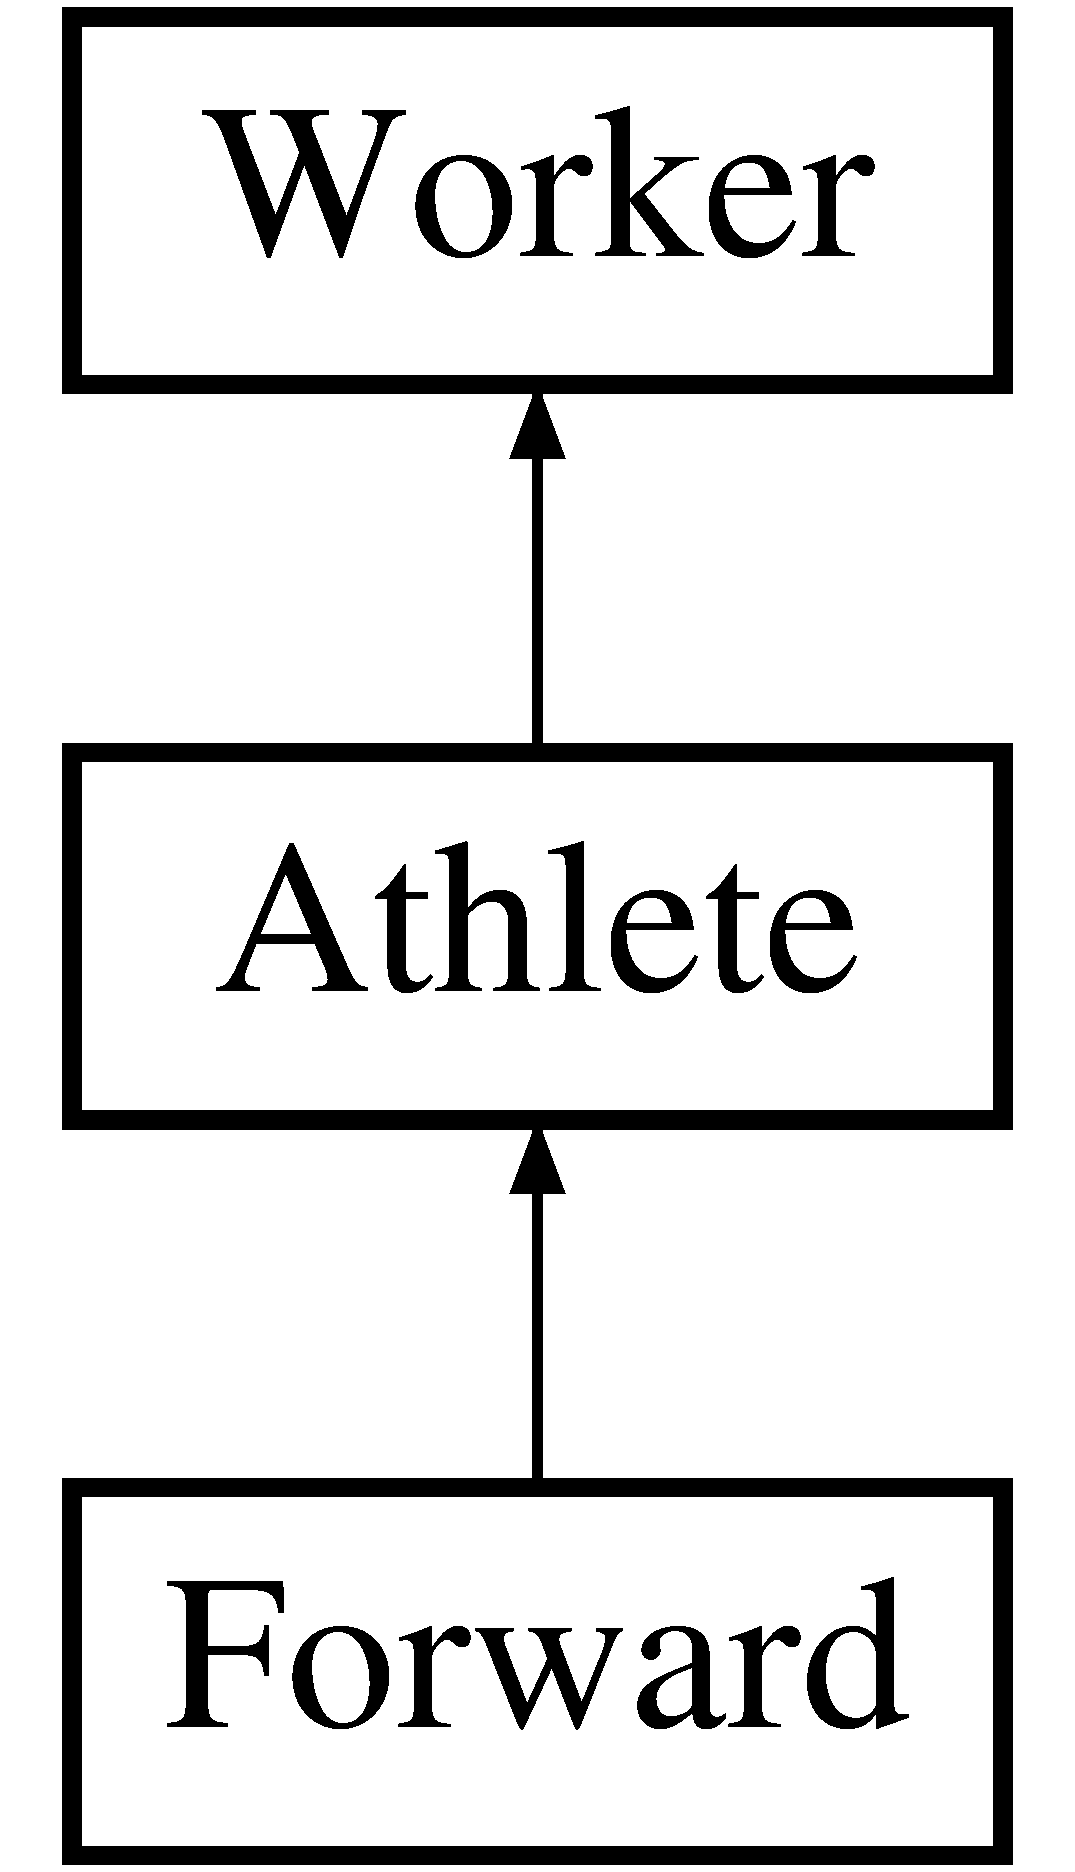
\includegraphics[height=3.000000cm]{class_forward}
\end{center}
\end{figure}
\subsection*{Public Member Functions}
\begin{DoxyCompactItemize}
\item 
\hyperlink{class_forward_ae7ea8d219a77c8b1fdb48bd2f9ef216b}{Forward} (string \hyperlink{class_worker_a66cf57341253a31e418cf8abad59ffb1}{name}, \hyperlink{class_date}{Date} \hyperlink{class_worker_a3c1845f40a084b471750a787a87614dd}{birthdate}, unsigned int \hyperlink{class_worker_adfafba55f967994f4595bd914bbba127}{civil\+ID}, unsigned char \hyperlink{class_athlete_a80a64bb1d5c943aaa7ca152d596d9914}{height}, unsigned \hyperlink{class_worker_afc39287cd510977cfe7697ed2c86b2ca}{id}=0)
\begin{DoxyCompactList}\small\item\em Constructor. The id is set automatically \end{DoxyCompactList}\item 
\hyperlink{class_forward_a2b053b5babe85f26e06a9da516903f6b}{Forward} (string \&new\+FW)
\begin{DoxyCompactList}\small\item\em Constructor that reads from the athletes file \end{DoxyCompactList}\item 
\hyperlink{class_forward_af018f03fdfd0e58c653bbb8411b77ef0}{$\sim$\+Forward} ()
\begin{DoxyCompactList}\small\item\em Destructor. \end{DoxyCompactList}\item 
unsigned int \hyperlink{class_forward_aacec6cafa4f965940286bd81e91e1eed}{get\+ID} () const
\begin{DoxyCompactList}\small\item\em Gets the forward\textquotesingle{}s identifier. \end{DoxyCompactList}\item 
\hyperlink{class_info}{Info} $\ast$ \hyperlink{class_forward_a5d8e8085c9a8c95a3296afc40fca81e5}{get\+Info} () const
\begin{DoxyCompactList}\small\item\em Gets the forward\textquotesingle{}s performance information. \end{DoxyCompactList}\item 
void \hyperlink{class_forward_a18f2db8a8234912d6a27727cb3b04fd9}{add\+Info} (\hyperlink{class_info}{Info} $\ast$more\+Info)
\begin{DoxyCompactList}\small\item\em Adds performance information to the forward. \end{DoxyCompactList}\end{DoxyCompactItemize}
\subsection*{Private Attributes}
\begin{DoxyCompactItemize}
\item 
\hyperlink{class_info}{Info} $\ast$ \hyperlink{class_forward_a64b43b34683be63ca7c8313ae755e4f0}{general\+Info}
\begin{DoxyCompactList}\small\item\em forward\textquotesingle{}s general information. \end{DoxyCompactList}\end{DoxyCompactItemize}
\subsection*{Additional Inherited Members}


\subsection{Detailed Description}
A forward. 

Lu�s, 20/11/2016. 

\subsection{Constructor \& Destructor Documentation}
\hypertarget{class_forward_ae7ea8d219a77c8b1fdb48bd2f9ef216b}{}\label{class_forward_ae7ea8d219a77c8b1fdb48bd2f9ef216b} 
\index{Forward@{Forward}!Forward@{Forward}}
\index{Forward@{Forward}!Forward@{Forward}}
\subsubsection{\texorpdfstring{Forward()}{Forward()}\hspace{0.1cm}{\footnotesize\ttfamily [1/2]}}
{\footnotesize\ttfamily Forward\+::\+Forward (\begin{DoxyParamCaption}\item[{string}]{name,  }\item[{\hyperlink{class_date}{Date}}]{birthdate,  }\item[{unsigned int}]{civil\+ID,  }\item[{unsigned char}]{height,  }\item[{unsigned}]{id = {\ttfamily 0} }\end{DoxyParamCaption})}



Constructor. The id is set automatically 

Lu�s, 20/11/2016. 


\begin{DoxyParams}{Parameters}
{\em name} & The name. \\
\hline
{\em birthdate} & The birthdate. \\
\hline
{\em civil\+ID} & Civil identifier. \\
\hline
{\em height} & The height. \\
\hline
\end{DoxyParams}
\hypertarget{class_forward_a2b053b5babe85f26e06a9da516903f6b}{}\label{class_forward_a2b053b5babe85f26e06a9da516903f6b} 
\index{Forward@{Forward}!Forward@{Forward}}
\index{Forward@{Forward}!Forward@{Forward}}
\subsubsection{\texorpdfstring{Forward()}{Forward()}\hspace{0.1cm}{\footnotesize\ttfamily [2/2]}}
{\footnotesize\ttfamily Forward\+::\+Forward (\begin{DoxyParamCaption}\item[{string \&}]{new\+FW }\end{DoxyParamCaption})}



Constructor that reads from the athletes file 

Lu�s, 20/11/2016. 


\begin{DoxyParams}{Parameters}
{\em new\+FW} & \mbox{[}in,out\mbox{]} The new firmware. \\
\hline
\end{DoxyParams}
\hypertarget{class_forward_af018f03fdfd0e58c653bbb8411b77ef0}{}\label{class_forward_af018f03fdfd0e58c653bbb8411b77ef0} 
\index{Forward@{Forward}!````~Forward@{$\sim$\+Forward}}
\index{````~Forward@{$\sim$\+Forward}!Forward@{Forward}}
\subsubsection{\texorpdfstring{$\sim$\+Forward()}{~Forward()}}
{\footnotesize\ttfamily Forward\+::$\sim$\+Forward (\begin{DoxyParamCaption}{ }\end{DoxyParamCaption})}



Destructor. 

Lu�s, 20/11/2016. 

\subsection{Member Function Documentation}
\hypertarget{class_forward_a18f2db8a8234912d6a27727cb3b04fd9}{}\label{class_forward_a18f2db8a8234912d6a27727cb3b04fd9} 
\index{Forward@{Forward}!add\+Info@{add\+Info}}
\index{add\+Info@{add\+Info}!Forward@{Forward}}
\subsubsection{\texorpdfstring{add\+Info()}{addInfo()}}
{\footnotesize\ttfamily void Forward\+::add\+Info (\begin{DoxyParamCaption}\item[{\hyperlink{class_info}{Info} $\ast$}]{more\+Info }\end{DoxyParamCaption})\hspace{0.3cm}{\ttfamily [virtual]}}



Adds performance information to the forward. 

This is a method that adds information to the forward

Lu�s, 20/11/2016. 


\begin{DoxyParams}{Parameters}
{\em more\+Info} & \mbox{[}in,out\mbox{]} If non-\/null, forward\textquotesingle{}s performance information. \\
\hline
\end{DoxyParams}


Reimplemented from \hyperlink{class_worker_ad54db262f7473cc729c371dd54e292eb}{Worker}.

\hypertarget{class_forward_aacec6cafa4f965940286bd81e91e1eed}{}\label{class_forward_aacec6cafa4f965940286bd81e91e1eed} 
\index{Forward@{Forward}!get\+ID@{get\+ID}}
\index{get\+ID@{get\+ID}!Forward@{Forward}}
\subsubsection{\texorpdfstring{get\+I\+D()}{getID()}}
{\footnotesize\ttfamily unsigned int Forward\+::get\+ID (\begin{DoxyParamCaption}{ }\end{DoxyParamCaption}) const\hspace{0.3cm}{\ttfamily [virtual]}}



Gets the forward\textquotesingle{}s identifier. 

Lu�s, 20/11/2016. 

\begin{DoxyReturn}{Returns}
The forward\textquotesingle{}s identifier. 
\end{DoxyReturn}


Implements \hyperlink{class_worker_a8b3e221c4a1ebd12ade03ee9b9c86182}{Worker}.

\hypertarget{class_forward_a5d8e8085c9a8c95a3296afc40fca81e5}{}\label{class_forward_a5d8e8085c9a8c95a3296afc40fca81e5} 
\index{Forward@{Forward}!get\+Info@{get\+Info}}
\index{get\+Info@{get\+Info}!Forward@{Forward}}
\subsubsection{\texorpdfstring{get\+Info()}{getInfo()}}
{\footnotesize\ttfamily \hyperlink{class_info}{Info} $\ast$ Forward\+::get\+Info (\begin{DoxyParamCaption}{ }\end{DoxyParamCaption}) const\hspace{0.3cm}{\ttfamily [virtual]}}



Gets the forward\textquotesingle{}s performance information. 

Lu�s, 20/11/2016. 

\begin{DoxyReturn}{Returns}
Null if it fails, else the forward\textquotesingle{}s performance information. 
\end{DoxyReturn}


Reimplemented from \hyperlink{class_worker_a95a4f7c750644937859b8e14515a480e}{Worker}.



\subsection{Member Data Documentation}
\hypertarget{class_forward_a64b43b34683be63ca7c8313ae755e4f0}{}\label{class_forward_a64b43b34683be63ca7c8313ae755e4f0} 
\index{Forward@{Forward}!general\+Info@{general\+Info}}
\index{general\+Info@{general\+Info}!Forward@{Forward}}
\subsubsection{\texorpdfstring{general\+Info}{generalInfo}}
{\footnotesize\ttfamily \hyperlink{class_info}{Info}$\ast$ Forward\+::general\+Info\hspace{0.3cm}{\ttfamily [private]}}



forward\textquotesingle{}s general information. 



The documentation for this class was generated from the following files\+:\begin{DoxyCompactItemize}
\item 
\hyperlink{_forward_8hpp}{Forward.\+hpp}\item 
\hyperlink{_forward_8cpp}{Forward.\+cpp}\end{DoxyCompactItemize}

\hypertarget{class_fraction}{}\section{Fraction Class Reference}
\label{class_fraction}\index{Fraction@{Fraction}}


{\ttfamily \#include $<$Utils.\+hpp$>$}

\subsection*{Public Member Functions}
\begin{DoxyCompactItemize}
\item 
\hyperlink{class_fraction_a29efaf0ef03cceab0bfa637e9eea2b7b}{Fraction} ()
\item 
\hyperlink{class_fraction_a55b666fe7b94b74f21d4919d9110805d}{Fraction} (int num, int den)
\item 
\hyperlink{class_fraction_a679e4834d2576a2b96a2904a81e5d990}{Fraction} (string fraction\+String)
\item 
\hyperlink{class_fraction}{Fraction} \hyperlink{class_fraction_ab72bc0a193460150fed673962f0681b9}{operator+} (\hyperlink{class_fraction}{Fraction} value) const
\item 
void \hyperlink{class_fraction_ad2327333e6f9186984eb728a9243ad1a}{operator+=} (\hyperlink{class_fraction}{Fraction} \&value)
\item 
\hyperlink{class_fraction}{Fraction} \hyperlink{class_fraction_a3ab475288d23337521e46c849bd81a88}{operator-\/} (\hyperlink{class_fraction}{Fraction} value) const
\item 
void \hyperlink{class_fraction_a560957bfe9353cfee0a6d30dbf66fb6f}{operator-\/=} (\hyperlink{class_fraction}{Fraction} \&value)
\item 
\hyperlink{class_fraction}{Fraction} \hyperlink{class_fraction_a88635ae851c5f33fe0c313319303220b}{operator$\ast$} (\hyperlink{class_fraction}{Fraction} value) const
\item 
void \hyperlink{class_fraction_a17225bab7600e54903a4716d21f6186b}{operator$\ast$=} (\hyperlink{class_fraction}{Fraction} \&value)
\item 
\hyperlink{class_fraction}{Fraction} \hyperlink{class_fraction_a60479946006e920343c3e03ce9f4f0f2}{operator/} (\hyperlink{class_fraction}{Fraction} value) const
\item 
void \hyperlink{class_fraction_a4a70499be6c756cf4e0f3982bb2558df}{operator/=} (\hyperlink{class_fraction}{Fraction} \&value)
\item 
bool \hyperlink{class_fraction_a7a122e21981f269280383178adce2868}{operator$<$} (\hyperlink{class_fraction}{Fraction} value) const
\item 
bool \hyperlink{class_fraction_ac652d0394b5c8f0046a975bf7ea1b60b}{operator==} (\hyperlink{class_fraction}{Fraction} value) const
\item 
bool \hyperlink{class_fraction_a2fc5da88a8106c34bd15a472c58cd61c}{operator$>$=} (\hyperlink{class_fraction}{Fraction} value) const
\item 
bool \hyperlink{class_fraction_a110a04c675b4737f09e6b84236f3d8e6}{operator$>$} (\hyperlink{class_fraction}{Fraction} value) const
\item 
bool \hyperlink{class_fraction_aa1a199c08a893bfb787a5b5a9915ba8b}{operator$<$=} (\hyperlink{class_fraction}{Fraction} value) const
\item 
\hyperlink{class_fraction}{Fraction} \hyperlink{class_fraction_a41a3516a3b2d8c431ea8a17a033f48a9}{operator$\vert$} (\hyperlink{class_fraction}{Fraction} value) const
\item 
void \hyperlink{class_fraction_a13da35dc2c6c3bee73c749192a61df8a}{operator$\vert$=} (const \hyperlink{class_fraction}{Fraction} \&value)
\item 
\hyperlink{class_fraction}{Fraction} \& \hyperlink{class_fraction_ac8ae2e81294340889183951be2657633}{operator++} ()
\item 
\hyperlink{class_fraction}{Fraction} \hyperlink{class_fraction_a8fc2c460f8cf333d153da2f53a969edf}{operator++} (int)
\item 
void \hyperlink{class_fraction_a8eee4d9ddb8a3484930f7fa5f7ca3ae7}{reduce} ()
\item 
void \hyperlink{class_fraction_a053300eed15ed1783a4316f9b7bf8a4f}{print} (bool original\+Fraction=true) const
\item 
void \hyperlink{class_fraction_a08ffc86159f5b96b10df4bfdf2f5c0a5}{print\+Percentage} () const
\item 
string \hyperlink{class_fraction_af475a2e5500fd3a0c36d918a2950464c}{get\+Frac} () const
\end{DoxyCompactItemize}
\subsection*{Private Attributes}
\begin{DoxyCompactItemize}
\item 
int \hyperlink{class_fraction_a447e179720bd927a19c1d73fb040d1c4}{numerator}
\item 
int \hyperlink{class_fraction_a079acff7892d39be395f14799244d044}{denominator}
\end{DoxyCompactItemize}


\subsection{Constructor \& Destructor Documentation}
\hypertarget{class_fraction_a29efaf0ef03cceab0bfa637e9eea2b7b}{}\label{class_fraction_a29efaf0ef03cceab0bfa637e9eea2b7b} 
\index{Fraction@{Fraction}!Fraction@{Fraction}}
\index{Fraction@{Fraction}!Fraction@{Fraction}}
\subsubsection{\texorpdfstring{Fraction()}{Fraction()}\hspace{0.1cm}{\footnotesize\ttfamily [1/3]}}
{\footnotesize\ttfamily Fraction\+::\+Fraction (\begin{DoxyParamCaption}{ }\end{DoxyParamCaption})}

\hypertarget{class_fraction_a55b666fe7b94b74f21d4919d9110805d}{}\label{class_fraction_a55b666fe7b94b74f21d4919d9110805d} 
\index{Fraction@{Fraction}!Fraction@{Fraction}}
\index{Fraction@{Fraction}!Fraction@{Fraction}}
\subsubsection{\texorpdfstring{Fraction()}{Fraction()}\hspace{0.1cm}{\footnotesize\ttfamily [2/3]}}
{\footnotesize\ttfamily Fraction\+::\+Fraction (\begin{DoxyParamCaption}\item[{int}]{num,  }\item[{int}]{den }\end{DoxyParamCaption})}

\hypertarget{class_fraction_a679e4834d2576a2b96a2904a81e5d990}{}\label{class_fraction_a679e4834d2576a2b96a2904a81e5d990} 
\index{Fraction@{Fraction}!Fraction@{Fraction}}
\index{Fraction@{Fraction}!Fraction@{Fraction}}
\subsubsection{\texorpdfstring{Fraction()}{Fraction()}\hspace{0.1cm}{\footnotesize\ttfamily [3/3]}}
{\footnotesize\ttfamily Fraction\+::\+Fraction (\begin{DoxyParamCaption}\item[{string}]{fraction\+String }\end{DoxyParamCaption})}



\subsection{Member Function Documentation}
\hypertarget{class_fraction_af475a2e5500fd3a0c36d918a2950464c}{}\label{class_fraction_af475a2e5500fd3a0c36d918a2950464c} 
\index{Fraction@{Fraction}!get\+Frac@{get\+Frac}}
\index{get\+Frac@{get\+Frac}!Fraction@{Fraction}}
\subsubsection{\texorpdfstring{get\+Frac()}{getFrac()}}
{\footnotesize\ttfamily string Fraction\+::get\+Frac (\begin{DoxyParamCaption}{ }\end{DoxyParamCaption}) const}

\hypertarget{class_fraction_a88635ae851c5f33fe0c313319303220b}{}\label{class_fraction_a88635ae851c5f33fe0c313319303220b} 
\index{Fraction@{Fraction}!operator$\ast$@{operator$\ast$}}
\index{operator$\ast$@{operator$\ast$}!Fraction@{Fraction}}
\subsubsection{\texorpdfstring{operator$\ast$()}{operator*()}}
{\footnotesize\ttfamily \hyperlink{class_fraction}{Fraction} Fraction\+::operator$\ast$ (\begin{DoxyParamCaption}\item[{\hyperlink{class_fraction}{Fraction}}]{value }\end{DoxyParamCaption}) const}

\hypertarget{class_fraction_a17225bab7600e54903a4716d21f6186b}{}\label{class_fraction_a17225bab7600e54903a4716d21f6186b} 
\index{Fraction@{Fraction}!operator$\ast$=@{operator$\ast$=}}
\index{operator$\ast$=@{operator$\ast$=}!Fraction@{Fraction}}
\subsubsection{\texorpdfstring{operator$\ast$=()}{operator*=()}}
{\footnotesize\ttfamily void Fraction\+::operator$\ast$= (\begin{DoxyParamCaption}\item[{\hyperlink{class_fraction}{Fraction} \&}]{value }\end{DoxyParamCaption})}

\hypertarget{class_fraction_ab72bc0a193460150fed673962f0681b9}{}\label{class_fraction_ab72bc0a193460150fed673962f0681b9} 
\index{Fraction@{Fraction}!operator+@{operator+}}
\index{operator+@{operator+}!Fraction@{Fraction}}
\subsubsection{\texorpdfstring{operator+()}{operator+()}}
{\footnotesize\ttfamily \hyperlink{class_fraction}{Fraction} Fraction\+::operator+ (\begin{DoxyParamCaption}\item[{\hyperlink{class_fraction}{Fraction}}]{value }\end{DoxyParamCaption}) const}

\hypertarget{class_fraction_ac8ae2e81294340889183951be2657633}{}\label{class_fraction_ac8ae2e81294340889183951be2657633} 
\index{Fraction@{Fraction}!operator++@{operator++}}
\index{operator++@{operator++}!Fraction@{Fraction}}
\subsubsection{\texorpdfstring{operator++()}{operator++()}\hspace{0.1cm}{\footnotesize\ttfamily [1/2]}}
{\footnotesize\ttfamily \hyperlink{class_fraction}{Fraction} \& Fraction\+::operator++ (\begin{DoxyParamCaption}{ }\end{DoxyParamCaption})}

\hypertarget{class_fraction_a8fc2c460f8cf333d153da2f53a969edf}{}\label{class_fraction_a8fc2c460f8cf333d153da2f53a969edf} 
\index{Fraction@{Fraction}!operator++@{operator++}}
\index{operator++@{operator++}!Fraction@{Fraction}}
\subsubsection{\texorpdfstring{operator++()}{operator++()}\hspace{0.1cm}{\footnotesize\ttfamily [2/2]}}
{\footnotesize\ttfamily \hyperlink{class_fraction}{Fraction} Fraction\+::operator++ (\begin{DoxyParamCaption}\item[{int}]{ }\end{DoxyParamCaption})}

\hypertarget{class_fraction_ad2327333e6f9186984eb728a9243ad1a}{}\label{class_fraction_ad2327333e6f9186984eb728a9243ad1a} 
\index{Fraction@{Fraction}!operator+=@{operator+=}}
\index{operator+=@{operator+=}!Fraction@{Fraction}}
\subsubsection{\texorpdfstring{operator+=()}{operator+=()}}
{\footnotesize\ttfamily void Fraction\+::operator+= (\begin{DoxyParamCaption}\item[{\hyperlink{class_fraction}{Fraction} \&}]{value }\end{DoxyParamCaption})}

\hypertarget{class_fraction_a3ab475288d23337521e46c849bd81a88}{}\label{class_fraction_a3ab475288d23337521e46c849bd81a88} 
\index{Fraction@{Fraction}!operator-\/@{operator-\/}}
\index{operator-\/@{operator-\/}!Fraction@{Fraction}}
\subsubsection{\texorpdfstring{operator-\/()}{operator-()}}
{\footnotesize\ttfamily \hyperlink{class_fraction}{Fraction} Fraction\+::operator-\/ (\begin{DoxyParamCaption}\item[{\hyperlink{class_fraction}{Fraction}}]{value }\end{DoxyParamCaption}) const}

\hypertarget{class_fraction_a560957bfe9353cfee0a6d30dbf66fb6f}{}\label{class_fraction_a560957bfe9353cfee0a6d30dbf66fb6f} 
\index{Fraction@{Fraction}!operator-\/=@{operator-\/=}}
\index{operator-\/=@{operator-\/=}!Fraction@{Fraction}}
\subsubsection{\texorpdfstring{operator-\/=()}{operator-=()}}
{\footnotesize\ttfamily void Fraction\+::operator-\/= (\begin{DoxyParamCaption}\item[{\hyperlink{class_fraction}{Fraction} \&}]{value }\end{DoxyParamCaption})}

\hypertarget{class_fraction_a60479946006e920343c3e03ce9f4f0f2}{}\label{class_fraction_a60479946006e920343c3e03ce9f4f0f2} 
\index{Fraction@{Fraction}!operator/@{operator/}}
\index{operator/@{operator/}!Fraction@{Fraction}}
\subsubsection{\texorpdfstring{operator/()}{operator/()}}
{\footnotesize\ttfamily \hyperlink{class_fraction}{Fraction} Fraction\+::operator/ (\begin{DoxyParamCaption}\item[{\hyperlink{class_fraction}{Fraction}}]{value }\end{DoxyParamCaption}) const}

\hypertarget{class_fraction_a4a70499be6c756cf4e0f3982bb2558df}{}\label{class_fraction_a4a70499be6c756cf4e0f3982bb2558df} 
\index{Fraction@{Fraction}!operator/=@{operator/=}}
\index{operator/=@{operator/=}!Fraction@{Fraction}}
\subsubsection{\texorpdfstring{operator/=()}{operator/=()}}
{\footnotesize\ttfamily void Fraction\+::operator/= (\begin{DoxyParamCaption}\item[{\hyperlink{class_fraction}{Fraction} \&}]{value }\end{DoxyParamCaption})}

\hypertarget{class_fraction_a7a122e21981f269280383178adce2868}{}\label{class_fraction_a7a122e21981f269280383178adce2868} 
\index{Fraction@{Fraction}!operator$<$@{operator$<$}}
\index{operator$<$@{operator$<$}!Fraction@{Fraction}}
\subsubsection{\texorpdfstring{operator$<$()}{operator<()}}
{\footnotesize\ttfamily bool Fraction\+::operator$<$ (\begin{DoxyParamCaption}\item[{\hyperlink{class_fraction}{Fraction}}]{value }\end{DoxyParamCaption}) const}

\hypertarget{class_fraction_aa1a199c08a893bfb787a5b5a9915ba8b}{}\label{class_fraction_aa1a199c08a893bfb787a5b5a9915ba8b} 
\index{Fraction@{Fraction}!operator$<$=@{operator$<$=}}
\index{operator$<$=@{operator$<$=}!Fraction@{Fraction}}
\subsubsection{\texorpdfstring{operator$<$=()}{operator<=()}}
{\footnotesize\ttfamily bool Fraction\+::operator$<$= (\begin{DoxyParamCaption}\item[{\hyperlink{class_fraction}{Fraction}}]{value }\end{DoxyParamCaption}) const}

\hypertarget{class_fraction_ac652d0394b5c8f0046a975bf7ea1b60b}{}\label{class_fraction_ac652d0394b5c8f0046a975bf7ea1b60b} 
\index{Fraction@{Fraction}!operator==@{operator==}}
\index{operator==@{operator==}!Fraction@{Fraction}}
\subsubsection{\texorpdfstring{operator==()}{operator==()}}
{\footnotesize\ttfamily bool Fraction\+::operator== (\begin{DoxyParamCaption}\item[{\hyperlink{class_fraction}{Fraction}}]{value }\end{DoxyParamCaption}) const}

\hypertarget{class_fraction_a110a04c675b4737f09e6b84236f3d8e6}{}\label{class_fraction_a110a04c675b4737f09e6b84236f3d8e6} 
\index{Fraction@{Fraction}!operator$>$@{operator$>$}}
\index{operator$>$@{operator$>$}!Fraction@{Fraction}}
\subsubsection{\texorpdfstring{operator$>$()}{operator>()}}
{\footnotesize\ttfamily bool Fraction\+::operator$>$ (\begin{DoxyParamCaption}\item[{\hyperlink{class_fraction}{Fraction}}]{value }\end{DoxyParamCaption}) const}

\hypertarget{class_fraction_a2fc5da88a8106c34bd15a472c58cd61c}{}\label{class_fraction_a2fc5da88a8106c34bd15a472c58cd61c} 
\index{Fraction@{Fraction}!operator$>$=@{operator$>$=}}
\index{operator$>$=@{operator$>$=}!Fraction@{Fraction}}
\subsubsection{\texorpdfstring{operator$>$=()}{operator>=()}}
{\footnotesize\ttfamily bool Fraction\+::operator$>$= (\begin{DoxyParamCaption}\item[{\hyperlink{class_fraction}{Fraction}}]{value }\end{DoxyParamCaption}) const}

\hypertarget{class_fraction_a41a3516a3b2d8c431ea8a17a033f48a9}{}\label{class_fraction_a41a3516a3b2d8c431ea8a17a033f48a9} 
\index{Fraction@{Fraction}!operator\texttt{"|}@{operator\texttt{"|}}}
\index{operator\texttt{"|}@{operator\texttt{"|}}!Fraction@{Fraction}}
\subsubsection{\texorpdfstring{operator\texttt{"|}()}{operator|()}}
{\footnotesize\ttfamily \hyperlink{class_fraction}{Fraction} Fraction\+::operator$\vert$ (\begin{DoxyParamCaption}\item[{\hyperlink{class_fraction}{Fraction}}]{value }\end{DoxyParamCaption}) const}

\hypertarget{class_fraction_a13da35dc2c6c3bee73c749192a61df8a}{}\label{class_fraction_a13da35dc2c6c3bee73c749192a61df8a} 
\index{Fraction@{Fraction}!operator\texttt{"|}=@{operator\texttt{"|}=}}
\index{operator\texttt{"|}=@{operator\texttt{"|}=}!Fraction@{Fraction}}
\subsubsection{\texorpdfstring{operator\texttt{"|}=()}{operator|=()}}
{\footnotesize\ttfamily void Fraction\+::operator$\vert$= (\begin{DoxyParamCaption}\item[{const \hyperlink{class_fraction}{Fraction} \&}]{value }\end{DoxyParamCaption})}

\hypertarget{class_fraction_a053300eed15ed1783a4316f9b7bf8a4f}{}\label{class_fraction_a053300eed15ed1783a4316f9b7bf8a4f} 
\index{Fraction@{Fraction}!print@{print}}
\index{print@{print}!Fraction@{Fraction}}
\subsubsection{\texorpdfstring{print()}{print()}}
{\footnotesize\ttfamily void Fraction\+::print (\begin{DoxyParamCaption}\item[{bool}]{original\+Fraction = {\ttfamily true} }\end{DoxyParamCaption}) const}

\hypertarget{class_fraction_a08ffc86159f5b96b10df4bfdf2f5c0a5}{}\label{class_fraction_a08ffc86159f5b96b10df4bfdf2f5c0a5} 
\index{Fraction@{Fraction}!print\+Percentage@{print\+Percentage}}
\index{print\+Percentage@{print\+Percentage}!Fraction@{Fraction}}
\subsubsection{\texorpdfstring{print\+Percentage()}{printPercentage()}}
{\footnotesize\ttfamily void Fraction\+::print\+Percentage (\begin{DoxyParamCaption}{ }\end{DoxyParamCaption}) const}

\hypertarget{class_fraction_a8eee4d9ddb8a3484930f7fa5f7ca3ae7}{}\label{class_fraction_a8eee4d9ddb8a3484930f7fa5f7ca3ae7} 
\index{Fraction@{Fraction}!reduce@{reduce}}
\index{reduce@{reduce}!Fraction@{Fraction}}
\subsubsection{\texorpdfstring{reduce()}{reduce()}}
{\footnotesize\ttfamily void Fraction\+::reduce (\begin{DoxyParamCaption}{ }\end{DoxyParamCaption})}



\subsection{Member Data Documentation}
\hypertarget{class_fraction_a079acff7892d39be395f14799244d044}{}\label{class_fraction_a079acff7892d39be395f14799244d044} 
\index{Fraction@{Fraction}!denominator@{denominator}}
\index{denominator@{denominator}!Fraction@{Fraction}}
\subsubsection{\texorpdfstring{denominator}{denominator}}
{\footnotesize\ttfamily int Fraction\+::denominator\hspace{0.3cm}{\ttfamily [private]}}

\hypertarget{class_fraction_a447e179720bd927a19c1d73fb040d1c4}{}\label{class_fraction_a447e179720bd927a19c1d73fb040d1c4} 
\index{Fraction@{Fraction}!numerator@{numerator}}
\index{numerator@{numerator}!Fraction@{Fraction}}
\subsubsection{\texorpdfstring{numerator}{numerator}}
{\footnotesize\ttfamily int Fraction\+::numerator\hspace{0.3cm}{\ttfamily [private]}}



The documentation for this class was generated from the following files\+:\begin{DoxyCompactItemize}
\item 
\hyperlink{_utils_8hpp}{Utils.\+hpp}\item 
\hyperlink{_utils_8cpp}{Utils.\+cpp}\end{DoxyCompactItemize}

\hypertarget{class_goalkeeper}{}\section{Goalkeeper Class Reference}
\label{class_goalkeeper}\index{Goalkeeper@{Goalkeeper}}


{\ttfamily \#include $<$Goalkeeper.\+hpp$>$}

Inheritance diagram for Goalkeeper\+:\begin{figure}[H]
\begin{center}
\leavevmode
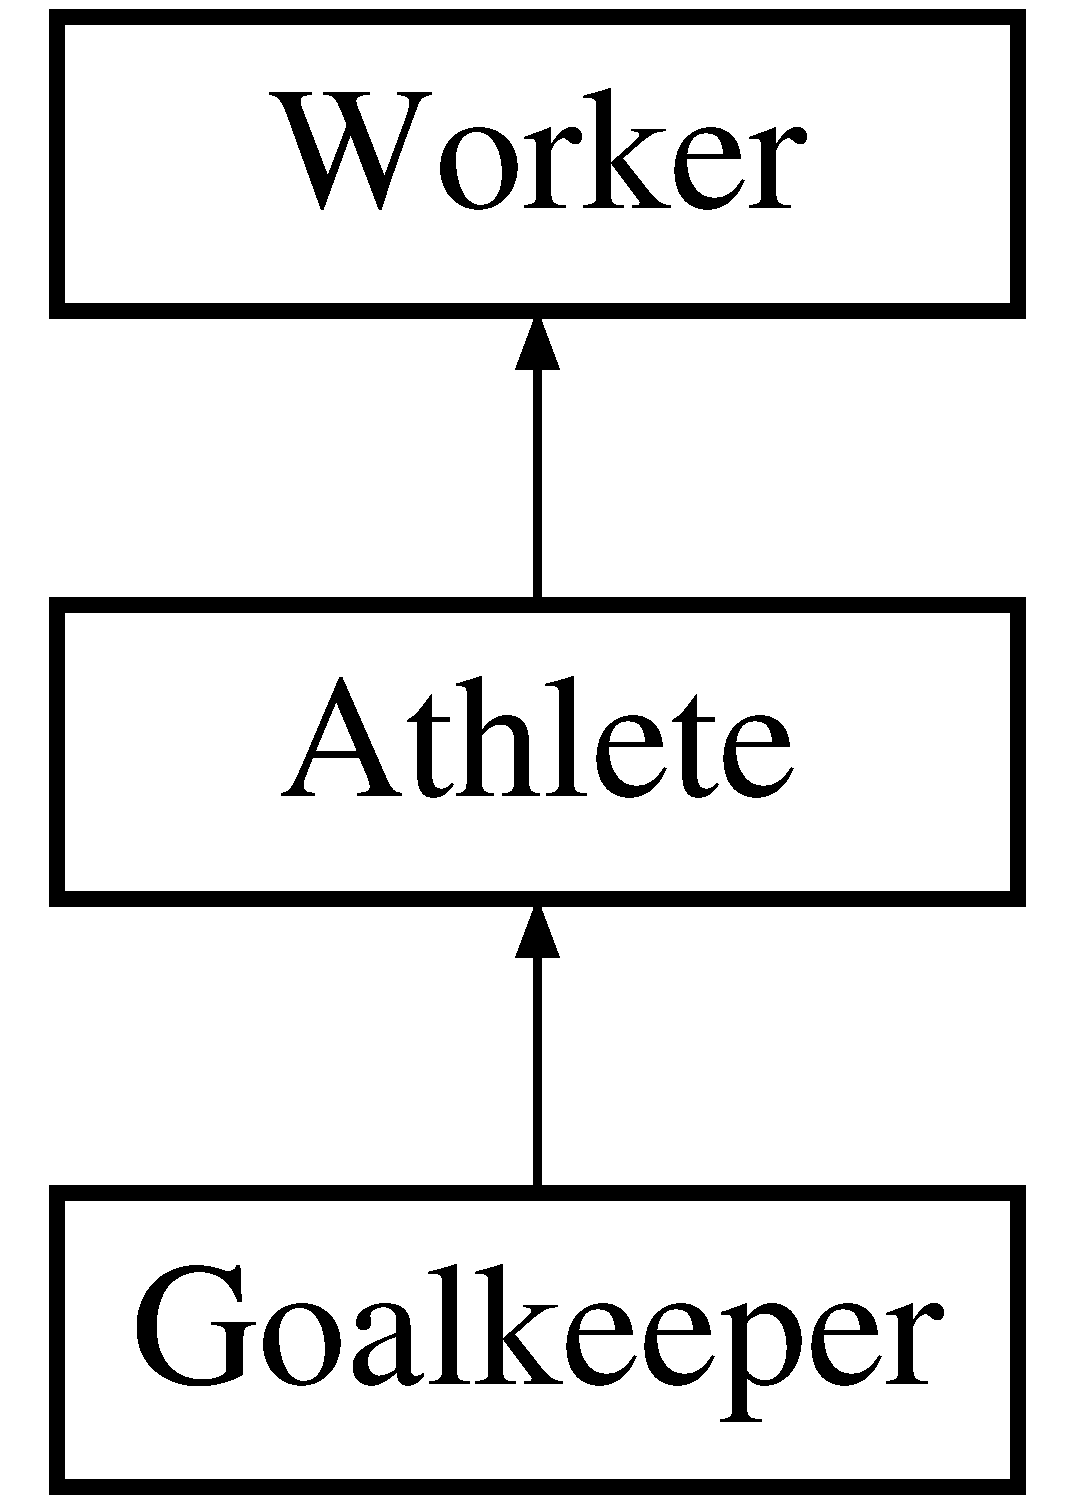
\includegraphics[height=3.000000cm]{class_goalkeeper}
\end{center}
\end{figure}
\subsection*{Public Member Functions}
\begin{DoxyCompactItemize}
\item 
\hyperlink{class_goalkeeper_a41b559a66be23a792b36e7872dedc58e}{Goalkeeper} (string \hyperlink{class_worker_a66cf57341253a31e418cf8abad59ffb1}{name}, \hyperlink{class_date}{Date} \hyperlink{class_worker_a3c1845f40a084b471750a787a87614dd}{birthdate}, unsigned int \hyperlink{class_worker_adfafba55f967994f4595bd914bbba127}{civil\+ID}, unsigned char \hyperlink{class_athlete_a80a64bb1d5c943aaa7ca152d596d9914}{height}, unsigned int=0)
\begin{DoxyCompactList}\small\item\em \hyperlink{class_goalkeeper}{Goalkeeper}\textquotesingle{}s constructors. \end{DoxyCompactList}\item 
\hyperlink{class_goalkeeper_aa5bf0b37a67658a7d8424efda7038a2c}{Goalkeeper} (string \&new\+GK)
\begin{DoxyCompactList}\small\item\em Constructor that creates a new goalkeeper by reading from the athletes file. \end{DoxyCompactList}\item 
\hyperlink{class_goalkeeper_ad06f685ef71e1c5b787088d9a327282a}{$\sim$\+Goalkeeper} ()
\begin{DoxyCompactList}\small\item\em Destructor. \end{DoxyCompactList}\item 
unsigned int \hyperlink{class_goalkeeper_a61cff0476146d2fc063d5ed7be82a123}{get\+ID} () const
\begin{DoxyCompactList}\small\item\em Gets the goalkeeper\textquotesingle{}s identifier. \end{DoxyCompactList}\item 
\hyperlink{class_info}{Info} $\ast$ \hyperlink{class_goalkeeper_a8636c061d81440070cf554d5a3923acb}{get\+Info} () const
\begin{DoxyCompactList}\small\item\em Gets the goalkeeper\textquotesingle{}s performance information. \end{DoxyCompactList}\item 
void \hyperlink{class_goalkeeper_a97fc43118c67d500d7d56abc9c0029fe}{add\+Info} (\hyperlink{class_info}{Info} $\ast$more\+Info)
\begin{DoxyCompactList}\small\item\em Adds performance information to the goalkeeper. \end{DoxyCompactList}\end{DoxyCompactItemize}
\subsection*{Private Attributes}
\begin{DoxyCompactItemize}
\item 
\hyperlink{class_info}{Info} $\ast$ \hyperlink{class_goalkeeper_a30367439b905583e7b5562d19ab531f3}{general\+Info}
\begin{DoxyCompactList}\small\item\em goalkeeper\textquotesingle{}s general info. \end{DoxyCompactList}\end{DoxyCompactItemize}
\subsection*{Additional Inherited Members}


\subsection{Constructor \& Destructor Documentation}
\hypertarget{class_goalkeeper_a41b559a66be23a792b36e7872dedc58e}{}\label{class_goalkeeper_a41b559a66be23a792b36e7872dedc58e} 
\index{Goalkeeper@{Goalkeeper}!Goalkeeper@{Goalkeeper}}
\index{Goalkeeper@{Goalkeeper}!Goalkeeper@{Goalkeeper}}
\subsubsection{\texorpdfstring{Goalkeeper()}{Goalkeeper()}\hspace{0.1cm}{\footnotesize\ttfamily [1/2]}}
{\footnotesize\ttfamily Goalkeeper\+::\+Goalkeeper (\begin{DoxyParamCaption}\item[{string}]{name,  }\item[{\hyperlink{class_date}{Date}}]{birthdate,  }\item[{unsigned int}]{civil\+ID,  }\item[{unsigned char}]{height,  }\item[{unsigned int}]{id = {\ttfamily 0} }\end{DoxyParamCaption})}



\hyperlink{class_goalkeeper}{Goalkeeper}\textquotesingle{}s constructors. 

This is a constructor that creates a new goalkeeper using his name, birthdate, civil\+ID and height. The id is set automatically 

Constructor. th id is set automatically 

Luís, 20/11/2016. 


\begin{DoxyParams}{Parameters}
{\em name} & The name. \\
\hline
{\em birthdate} & The birthdate. \\
\hline
{\em civil\+ID} & Identifier for the civil. \\
\hline
{\em height} & The height. \\
\hline
{\em int} & (Optional) The int. \\
\hline
\end{DoxyParams}
\hypertarget{class_goalkeeper_aa5bf0b37a67658a7d8424efda7038a2c}{}\label{class_goalkeeper_aa5bf0b37a67658a7d8424efda7038a2c} 
\index{Goalkeeper@{Goalkeeper}!Goalkeeper@{Goalkeeper}}
\index{Goalkeeper@{Goalkeeper}!Goalkeeper@{Goalkeeper}}
\subsubsection{\texorpdfstring{Goalkeeper()}{Goalkeeper()}\hspace{0.1cm}{\footnotesize\ttfamily [2/2]}}
{\footnotesize\ttfamily Goalkeeper\+::\+Goalkeeper (\begin{DoxyParamCaption}\item[{string \&}]{new\+GK }\end{DoxyParamCaption})}



Constructor that creates a new goalkeeper by reading from the athletes file. 

Luís, 20/11/2016. 


\begin{DoxyParams}{Parameters}
{\em new\+GK} & \mbox{[}in,out\mbox{]} The new goalkeeper. \\
\hline
\end{DoxyParams}
\hypertarget{class_goalkeeper_ad06f685ef71e1c5b787088d9a327282a}{}\label{class_goalkeeper_ad06f685ef71e1c5b787088d9a327282a} 
\index{Goalkeeper@{Goalkeeper}!````~Goalkeeper@{$\sim$\+Goalkeeper}}
\index{````~Goalkeeper@{$\sim$\+Goalkeeper}!Goalkeeper@{Goalkeeper}}
\subsubsection{\texorpdfstring{$\sim$\+Goalkeeper()}{~Goalkeeper()}}
{\footnotesize\ttfamily Goalkeeper\+::$\sim$\+Goalkeeper (\begin{DoxyParamCaption}{ }\end{DoxyParamCaption})}



Destructor. 

Luís, 20/11/2016. 

\subsection{Member Function Documentation}
\hypertarget{class_goalkeeper_a97fc43118c67d500d7d56abc9c0029fe}{}\label{class_goalkeeper_a97fc43118c67d500d7d56abc9c0029fe} 
\index{Goalkeeper@{Goalkeeper}!add\+Info@{add\+Info}}
\index{add\+Info@{add\+Info}!Goalkeeper@{Goalkeeper}}
\subsubsection{\texorpdfstring{add\+Info()}{addInfo()}}
{\footnotesize\ttfamily void Goalkeeper\+::add\+Info (\begin{DoxyParamCaption}\item[{\hyperlink{class_info}{Info} $\ast$}]{more\+Info }\end{DoxyParamCaption})\hspace{0.3cm}{\ttfamily [virtual]}}



Adds performance information to the goalkeeper. 

This is a method that adds information to the goalkeeper

Luís, 20/11/2016. 


\begin{DoxyParams}{Parameters}
{\em more\+Info} & \mbox{[}in,out\mbox{]} If non-\/null, goalkeeper\textquotesingle{}s performance information. \\
\hline
\end{DoxyParams}


Reimplemented from \hyperlink{class_worker_ad54db262f7473cc729c371dd54e292eb}{Worker}.

\hypertarget{class_goalkeeper_a61cff0476146d2fc063d5ed7be82a123}{}\label{class_goalkeeper_a61cff0476146d2fc063d5ed7be82a123} 
\index{Goalkeeper@{Goalkeeper}!get\+ID@{get\+ID}}
\index{get\+ID@{get\+ID}!Goalkeeper@{Goalkeeper}}
\subsubsection{\texorpdfstring{get\+I\+D()}{getID()}}
{\footnotesize\ttfamily unsigned int Goalkeeper\+::get\+ID (\begin{DoxyParamCaption}{ }\end{DoxyParamCaption}) const\hspace{0.3cm}{\ttfamily [virtual]}}



Gets the goalkeeper\textquotesingle{}s identifier. 

This is a method that gets the goalkeeper\textquotesingle{}s id

Luís, 20/11/2016. 

\begin{DoxyReturn}{Returns}
The goalkeeper\textquotesingle{}s identifier. 
\end{DoxyReturn}


Implements \hyperlink{class_worker_a8b3e221c4a1ebd12ade03ee9b9c86182}{Worker}.

\hypertarget{class_goalkeeper_a8636c061d81440070cf554d5a3923acb}{}\label{class_goalkeeper_a8636c061d81440070cf554d5a3923acb} 
\index{Goalkeeper@{Goalkeeper}!get\+Info@{get\+Info}}
\index{get\+Info@{get\+Info}!Goalkeeper@{Goalkeeper}}
\subsubsection{\texorpdfstring{get\+Info()}{getInfo()}}
{\footnotesize\ttfamily \hyperlink{class_info}{Info} $\ast$ Goalkeeper\+::get\+Info (\begin{DoxyParamCaption}{ }\end{DoxyParamCaption}) const\hspace{0.3cm}{\ttfamily [virtual]}}



Gets the goalkeeper\textquotesingle{}s performance information. 

This is a method that gets the goalkeeper\textquotesingle{}s performance information

Luís, 20/11/2016. 

\begin{DoxyReturn}{Returns}
Null if it fails, else the goalkeeper\textquotesingle{}s performance information. 
\end{DoxyReturn}


Reimplemented from \hyperlink{class_worker_a95a4f7c750644937859b8e14515a480e}{Worker}.



\subsection{Member Data Documentation}
\hypertarget{class_goalkeeper_a30367439b905583e7b5562d19ab531f3}{}\label{class_goalkeeper_a30367439b905583e7b5562d19ab531f3} 
\index{Goalkeeper@{Goalkeeper}!general\+Info@{general\+Info}}
\index{general\+Info@{general\+Info}!Goalkeeper@{Goalkeeper}}
\subsubsection{\texorpdfstring{general\+Info}{generalInfo}}
{\footnotesize\ttfamily \hyperlink{class_info}{Info}$\ast$ Goalkeeper\+::general\+Info\hspace{0.3cm}{\ttfamily [private]}}



goalkeeper\textquotesingle{}s general info. 



The documentation for this class was generated from the following files\+:\begin{DoxyCompactItemize}
\item 
\hyperlink{_goalkeeper_8hpp}{Goalkeeper.\+hpp}\item 
\hyperlink{_goalkeeper_8cpp}{Goalkeeper.\+cpp}\end{DoxyCompactItemize}

\hypertarget{class_info}{}\section{Info Class Reference}
\label{class_info}\index{Info@{Info}}


{\ttfamily \#include $<$Info\+Athletes.\+hpp$>$}

Inheritance diagram for Info\+:\begin{figure}[H]
\begin{center}
\leavevmode
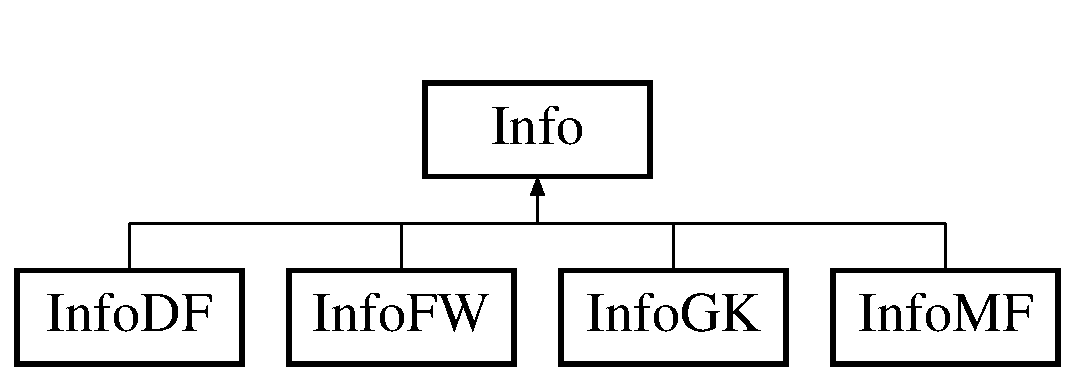
\includegraphics[height=2.000000cm]{class_info}
\end{center}
\end{figure}
\subsection*{Public Member Functions}
\begin{DoxyCompactItemize}
\item 
\hyperlink{class_info_a9eb23cc9b0bc2edee5977ec55f1717e2}{Info} (\hyperlink{class_fraction}{Fraction} \hyperlink{class_info_ae893be5aad319de5d911c3f80cc0a2d4}{training\+Freq}, unsigned int \hyperlink{class_info_aabdfdb282f3ceaae1772574bf2b3cd86}{yellow\+Cards}, unsigned int \hyperlink{class_info_a953c30accc7e6ff301542adfd5824f38}{red\+Cards}, unsigned int \hyperlink{class_info_aecdd57d96490b16a0c2590dd8f34009e}{tackles}, unsigned int \hyperlink{class_info_a2f90c84ba67c0e225dd58cdc14ab7f3d}{fouls}, unsigned int \hyperlink{class_info_a5ad5f72833856502b9c1f6ea50a98619}{goals\+Scored}, unsigned int \hyperlink{class_info_a1c0340af11df3407946b0ffdaae28864}{assists}, \hyperlink{class_fraction}{Fraction} \hyperlink{class_info_a37ee53dc8ae9a9656206e7eb389c6392}{pass\+Accuracy})
\begin{DoxyCompactList}\small\item\em \hyperlink{class_info}{Info} constructors. \end{DoxyCompactList}\item 
\hyperlink{class_info_a2c2d563e5bbaf12ece3b3de638f87a89}{Info} (string \&new\+Info)
\begin{DoxyCompactList}\small\item\em Constructor that creates new athlete\textquotesingle{}s performance information by reading it from athletes file using a string. \end{DoxyCompactList}\item 
\hyperlink{class_info_a89823cdd427a9dfdf3d2e43d938222bd}{Info} ()
\begin{DoxyCompactList}\small\item\em Default constructor. \end{DoxyCompactList}\item 
\hyperlink{class_info_a45dbc59e7e008bcc1849f0260ea2d64f}{Info} (istream \&in\+Stream)
\begin{DoxyCompactList}\small\item\em Constructor that creates new athlete\textquotesingle{}s performance information by reading it from thae athletes file using a stringstream. \end{DoxyCompactList}\item 
\hyperlink{class_fraction}{Fraction} \hyperlink{class_info_ace20d53ed24c8288e7e2fab3d4c4faa1}{get\+Training\+Freq} () const
\begin{DoxyCompactList}\small\item\em Gets the athlete\textquotesingle{}s training attendance. \end{DoxyCompactList}\item 
void \hyperlink{class_info_acbd13c7c7b330089ab211158a5bc6c13}{add\+Training} (\hyperlink{class_fraction}{Fraction} new\+Training=\hyperlink{class_fraction}{Fraction}(1, 1))
\begin{DoxyCompactList}\small\item\em Adds a training and calculates the athlete\textquotesingle{}s overall training attendance. \end{DoxyCompactList}\item 
unsigned int \hyperlink{class_info_ab357ec119b1281b94e37a1a853e1d149}{get\+Yellow\+Cards} () const
\begin{DoxyCompactList}\small\item\em Gets the athlete\textquotesingle{}s number of yellow cards. \end{DoxyCompactList}\item 
unsigned int \hyperlink{class_info_aac0891ef0f8767df1b5782ed108610de}{get\+Red\+Cards} () const
\begin{DoxyCompactList}\small\item\em Gets the athlete\textquotesingle{}s number of red cards. \end{DoxyCompactList}\item 
void \hyperlink{class_info_a414d2bf966a75da821b708bec2ec612d}{add\+Yellow\+Card} ()
\begin{DoxyCompactList}\small\item\em Adds a yellow card to the athlete\textquotesingle{}s total number of yellow cards. \end{DoxyCompactList}\item 
void \hyperlink{class_info_acbfe3707047b1a4f7b9b8442797cbaa3}{add\+Red\+Card} ()
\begin{DoxyCompactList}\small\item\em Adds a red card to the athlete\textquotesingle{}s total number of red cards. \end{DoxyCompactList}\item 
unsigned int \hyperlink{class_info_abab4dbd4bf56022685e1984fffb00c60}{get\+Tackles} () const
\begin{DoxyCompactList}\small\item\em Gets the number of tackles made by the athlete. \end{DoxyCompactList}\item 
void \hyperlink{class_info_a7d57f15ce5bf8b0b069d6f11c2238f36}{add\+Tackles} (unsigned int \hyperlink{class_info_aecdd57d96490b16a0c2590dd8f34009e}{tackles})
\begin{DoxyCompactList}\small\item\em Adds tackles to the total number of tackles made by the athlete. \end{DoxyCompactList}\item 
unsigned int \hyperlink{class_info_a94195f6bb305a247355f4038c18b3a67}{get\+Fouls} () const
\begin{DoxyCompactList}\small\item\em Gets the number of fouls commited by the athlete. \end{DoxyCompactList}\item 
void \hyperlink{class_info_aa4f58053aaff1dc1112f6c6396b64117}{add\+Fouls} (unsigned int \hyperlink{class_info_a2f90c84ba67c0e225dd58cdc14ab7f3d}{fouls})
\begin{DoxyCompactList}\small\item\em Adds fouls to the total number of fouls commited by the athlete. \end{DoxyCompactList}\item 
unsigned int \hyperlink{class_info_a2f29d691be81af12140d1bb88c9b7bad}{get\+Goals\+Scored} () const
\begin{DoxyCompactList}\small\item\em Gets the number of goals scored by the athlete. \end{DoxyCompactList}\item 
void \hyperlink{class_info_a19c376ed8c02c94f7836f1b61c0e1008}{add\+Goals\+Scored} (unsigned int \hyperlink{class_info_a5ad5f72833856502b9c1f6ea50a98619}{goals\+Scored})
\begin{DoxyCompactList}\small\item\em Adds goals to the total number of goals scored by the athlete. \end{DoxyCompactList}\item 
unsigned int \hyperlink{class_info_a38bd3c4f89a9b2f6d57ff7c3b7efa2ea}{get\+Assists} () const
\begin{DoxyCompactList}\small\item\em Gets the number of assists made by the athlete. \end{DoxyCompactList}\item 
void \hyperlink{class_info_accd8e297dc18e19d498376a2532c4862}{add\+Assists} (unsigned int \hyperlink{class_info_a1c0340af11df3407946b0ffdaae28864}{assists})
\begin{DoxyCompactList}\small\item\em Adds assists to the total number of assists made by the athlete. \end{DoxyCompactList}\item 
\hyperlink{class_fraction}{Fraction} \hyperlink{class_info_a8891b7452e20bac9e90f3501d39bdec8}{get\+Pass\+Accuracy} () const
\begin{DoxyCompactList}\small\item\em Gets pass accuracy. \end{DoxyCompactList}\item 
void \hyperlink{class_info_a6a37e09fc6160b19f3f7b480f77393dd}{add\+Pass\+Accuracy} (\hyperlink{class_fraction}{Fraction} \hyperlink{class_info_a37ee53dc8ae9a9656206e7eb389c6392}{pass\+Accuracy})
\begin{DoxyCompactList}\small\item\em Adds a new passing accuracy and calculates the athlete\textquotesingle{}s overall passing accuracy. \end{DoxyCompactList}\item 
virtual unsigned int \hyperlink{class_info_a2d7c53d322a705aaeb08fb79f9ef5211}{get\+Saves} () const
\begin{DoxyCompactList}\small\item\em Gets the number of saves made by the goalkeeper. \end{DoxyCompactList}\item 
virtual void \hyperlink{class_info_a7e66fc93d6ab97827bbf50fa61c71186}{add\+Saves} (unsigned int saves)
\begin{DoxyCompactList}\small\item\em Adds saves to the total number of saves made by the goalkeeper. \end{DoxyCompactList}\item 
virtual unsigned int \hyperlink{class_info_a41d954fad291a5ffdfe29cb1cf3f75ce}{get\+Goals\+Conceeded} () const
\begin{DoxyCompactList}\small\item\em Gets the number of goals conceeded by the goalkeeper. \end{DoxyCompactList}\item 
virtual void \hyperlink{class_info_ae252f25a8dff58017b92ba7a5ad02bc0}{add\+Goals\+Conceeded} (unsigned int goals\+Conceeded)
\begin{DoxyCompactList}\small\item\em Adds goals conceeded to total number of goals conceeded by the goalkeeper. \end{DoxyCompactList}\item 
virtual vector$<$ \hyperlink{_utils_8hpp_a94ee089ecd5db12c81c7edbefaabff4d}{Defender\+Position} $>$ \hyperlink{class_info_afa64d6a602f80674209e3391bf5fa309}{get\+Defender\+Specific\+Positions} () const
\begin{DoxyCompactList}\small\item\em Gets the vector containing the defender specific positions. \end{DoxyCompactList}\item 
virtual void \hyperlink{class_info_a33d98f07e5a276f9a3d0a08275f559b3}{add\+Defender\+Specific\+Position} (\hyperlink{_utils_8hpp_a94ee089ecd5db12c81c7edbefaabff4d}{Defender\+Position} new\+Pos)
\begin{DoxyCompactList}\small\item\em Adds a defender specific position to the vector containing the different positions of the defender. \end{DoxyCompactList}\item 
virtual vector$<$ \hyperlink{_utils_8hpp_a9f9328fe291d23e820ad594679abd217}{Midfielder\+Position} $>$ \hyperlink{class_info_afb5cbe001c15498897fc4852bd08c114}{get\+Midfielder\+Specific\+Positions} () const
\begin{DoxyCompactList}\small\item\em Gets the vector containing the midfielder specific positions. \end{DoxyCompactList}\item 
virtual void \hyperlink{class_info_ad90cc81b8a235763cf4127d90aa3a66a}{add\+Midfielder\+Specific\+Position} (\hyperlink{_utils_8hpp_a9f9328fe291d23e820ad594679abd217}{Midfielder\+Position} new\+Pos)
\begin{DoxyCompactList}\small\item\em Adds a midfielder specific position to the vector containing the different positions of the midfielder. \end{DoxyCompactList}\item 
virtual vector$<$ \hyperlink{_utils_8hpp_ae6ffae6f01bd3312aac4a44642f14620}{Forward\+Position} $>$ \hyperlink{class_info_abff2f6cd7a845b8bd80c97d9d456e07e}{get\+Forward\+Specific\+Positions} () const
\begin{DoxyCompactList}\small\item\em Gets the vector containing the forward specific positions. \end{DoxyCompactList}\item 
virtual void \hyperlink{class_info_afba094a1c19e8ff4bb3a9048ca6c7f4a}{add\+Attacker\+Specific\+Position} (\hyperlink{_utils_8hpp_ae6ffae6f01bd3312aac4a44642f14620}{Forward\+Position} new\+Pos)
\begin{DoxyCompactList}\small\item\em Adds an attacker specific position to the vector containing the different positions of the forward. \end{DoxyCompactList}\item 
virtual string \hyperlink{class_info_a5e52b35a9c17b58222bb57af16c16ce3}{generate\+String} () const
\begin{DoxyCompactList}\small\item\em Generates a string containing the athlete\textquotesingle{}s performance information. \end{DoxyCompactList}\item 
virtual void \hyperlink{class_info_a7b18f01c7cef1a219d3adb6677f3475f}{save} (ofstream \&out)
\begin{DoxyCompactList}\small\item\em Saves the athlete\textquotesingle{}s performance information into the athlete\textquotesingle{}s file using the overload of the operator$<$$<$, especified above. \end{DoxyCompactList}\item 
void \hyperlink{class_info_a9c2e39f8cfbe6d070d1154313fe0dd2e}{sum\+General\+Info} (const \hyperlink{class_info}{Info} \&info2)
\begin{DoxyCompactList}\small\item\em Adds two different blocks of athlete\textquotesingle{}s perfomance information, adding each atribute with the respective atribute of the other block. \end{DoxyCompactList}\item 
virtual void \hyperlink{class_info_a35d820d35f8ab3b8de15cdfc07f0c5a4}{operator+=} (const \hyperlink{class_info}{Info} $\ast$info2)
\begin{DoxyCompactList}\small\item\em Addition assignment operator. \end{DoxyCompactList}\end{DoxyCompactItemize}
\subsection*{Protected Attributes}
\begin{DoxyCompactItemize}
\item 
\hyperlink{class_fraction}{Fraction} \hyperlink{class_info_ae893be5aad319de5d911c3f80cc0a2d4}{training\+Freq}
\begin{DoxyCompactList}\small\item\em athlete\textquotesingle{}s training frequency percentage. \end{DoxyCompactList}\item 
unsigned int \hyperlink{class_info_aabdfdb282f3ceaae1772574bf2b3cd86}{yellow\+Cards}
\begin{DoxyCompactList}\small\item\em athlete\textquotesingle{}s number of yellow cards. \end{DoxyCompactList}\item 
unsigned int \hyperlink{class_info_a953c30accc7e6ff301542adfd5824f38}{red\+Cards}
\begin{DoxyCompactList}\small\item\em athlete\textquotesingle{}s number of red cards. \end{DoxyCompactList}\item 
unsigned int \hyperlink{class_info_aecdd57d96490b16a0c2590dd8f34009e}{tackles}
\begin{DoxyCompactList}\small\item\em athlete\textquotesingle{}s number of tackles. \end{DoxyCompactList}\item 
unsigned int \hyperlink{class_info_a2f90c84ba67c0e225dd58cdc14ab7f3d}{fouls}
\begin{DoxyCompactList}\small\item\em athlete\textquotesingle{}s number of fouls commited. \end{DoxyCompactList}\item 
unsigned int \hyperlink{class_info_a5ad5f72833856502b9c1f6ea50a98619}{goals\+Scored}
\begin{DoxyCompactList}\small\item\em athlete\textquotesingle{}s number of goals scored. \end{DoxyCompactList}\item 
unsigned int \hyperlink{class_info_a1c0340af11df3407946b0ffdaae28864}{assists}
\begin{DoxyCompactList}\small\item\em athlete\textquotesingle{}s number of assist made. \end{DoxyCompactList}\item 
\hyperlink{class_fraction}{Fraction} \hyperlink{class_info_a37ee53dc8ae9a9656206e7eb389c6392}{pass\+Accuracy}
\begin{DoxyCompactList}\small\item\em athlete\textquotesingle{}s pass accuracy percentage. \end{DoxyCompactList}\end{DoxyCompactItemize}
\subsection*{Friends}
\begin{DoxyCompactItemize}
\item 
ostream \& \hyperlink{class_info_afea35e873bef1ced055e4f0e3eee9838}{operator$<$$<$} (ostream \&out, const \hyperlink{class_info}{Info} \&info)
\begin{DoxyCompactList}\small\item\em Stream insertion operator that writes in the athlete\textquotesingle{}s file the string containing the athlete\textquotesingle{}s performance information generated in the virtual method \hyperlink{class_info_a5e52b35a9c17b58222bb57af16c16ce3}{generate\+String()}, using a stringstream. \end{DoxyCompactList}\end{DoxyCompactItemize}


\subsection{Constructor \& Destructor Documentation}
\hypertarget{class_info_a9eb23cc9b0bc2edee5977ec55f1717e2}{}\label{class_info_a9eb23cc9b0bc2edee5977ec55f1717e2} 
\index{Info@{Info}!Info@{Info}}
\index{Info@{Info}!Info@{Info}}
\subsubsection{\texorpdfstring{Info()}{Info()}\hspace{0.1cm}{\footnotesize\ttfamily [1/4]}}
{\footnotesize\ttfamily Info\+::\+Info (\begin{DoxyParamCaption}\item[{\hyperlink{class_fraction}{Fraction}}]{training\+Freq,  }\item[{unsigned int}]{yellow\+Cards,  }\item[{unsigned int}]{red\+Cards,  }\item[{unsigned int}]{tackles,  }\item[{unsigned int}]{fouls,  }\item[{unsigned int}]{goals\+Scored,  }\item[{unsigned int}]{assists,  }\item[{\hyperlink{class_fraction}{Fraction}}]{pass\+Accuracy }\end{DoxyParamCaption})}



\hyperlink{class_info}{Info} constructors. 

This is a constructor that creates new athlete\textquotesingle{}s performance information using training frequency, number of yellow cards, number of red cards, number of tackles, number of fouls commited, number of goals scored, number of assists, pass accuracy 

Constructor. 

Luís, 20/11/2016. 


\begin{DoxyParams}{Parameters}
{\em training\+Freq} & The training frequency. \\
\hline
{\em yellow\+Cards} & The yellow cards. \\
\hline
{\em red\+Cards} & The red cards. \\
\hline
{\em tackles} & The tackles. \\
\hline
{\em fouls} & The fouls. \\
\hline
{\em goals\+Scored} & The goals scored. \\
\hline
{\em assists} & The assists. \\
\hline
{\em pass\+Accuracy} & The pass accuracy. \\
\hline
\end{DoxyParams}
\hypertarget{class_info_a2c2d563e5bbaf12ece3b3de638f87a89}{}\label{class_info_a2c2d563e5bbaf12ece3b3de638f87a89} 
\index{Info@{Info}!Info@{Info}}
\index{Info@{Info}!Info@{Info}}
\subsubsection{\texorpdfstring{Info()}{Info()}\hspace{0.1cm}{\footnotesize\ttfamily [2/4]}}
{\footnotesize\ttfamily Info\+::\+Info (\begin{DoxyParamCaption}\item[{string \&}]{new\+Info }\end{DoxyParamCaption})}



Constructor that creates new athlete\textquotesingle{}s performance information by reading it from athletes file using a string. 

This is a constructor that creates new athlete\textquotesingle{}s performance information by reading it from athletes file using a string

Luís, 20/11/2016. 


\begin{DoxyParams}{Parameters}
{\em new\+Info} & \mbox{[}in,out\mbox{]} Information describing the new. \\
\hline
\end{DoxyParams}
\hypertarget{class_info_a89823cdd427a9dfdf3d2e43d938222bd}{}\label{class_info_a89823cdd427a9dfdf3d2e43d938222bd} 
\index{Info@{Info}!Info@{Info}}
\index{Info@{Info}!Info@{Info}}
\subsubsection{\texorpdfstring{Info()}{Info()}\hspace{0.1cm}{\footnotesize\ttfamily [3/4]}}
{\footnotesize\ttfamily Info\+::\+Info (\begin{DoxyParamCaption}{ }\end{DoxyParamCaption})}



Default constructor. 

Luís, 20/11/2016. \hypertarget{class_info_a45dbc59e7e008bcc1849f0260ea2d64f}{}\label{class_info_a45dbc59e7e008bcc1849f0260ea2d64f} 
\index{Info@{Info}!Info@{Info}}
\index{Info@{Info}!Info@{Info}}
\subsubsection{\texorpdfstring{Info()}{Info()}\hspace{0.1cm}{\footnotesize\ttfamily [4/4]}}
{\footnotesize\ttfamily Info\+::\+Info (\begin{DoxyParamCaption}\item[{istream \&}]{in\+Stream }\end{DoxyParamCaption})}



Constructor that creates new athlete\textquotesingle{}s performance information by reading it from thae athletes file using a stringstream. 

This is a constructor that creates new athlete\textquotesingle{}s performance information by reading it from thae athletes file using a stringstream

Luís, 20/11/2016. 


\begin{DoxyParams}{Parameters}
{\em in\+Stream} & \mbox{[}in,out\mbox{]} Data read from the athletes file. \\
\hline
\end{DoxyParams}


\subsection{Member Function Documentation}
\hypertarget{class_info_accd8e297dc18e19d498376a2532c4862}{}\label{class_info_accd8e297dc18e19d498376a2532c4862} 
\index{Info@{Info}!add\+Assists@{add\+Assists}}
\index{add\+Assists@{add\+Assists}!Info@{Info}}
\subsubsection{\texorpdfstring{add\+Assists()}{addAssists()}}
{\footnotesize\ttfamily void Info\+::add\+Assists (\begin{DoxyParamCaption}\item[{unsigned int}]{assists }\end{DoxyParamCaption})}



Adds assists to the total number of assists made by the athlete. 

This is a method that adds assists to the total number of assists made by the athlete

Luís, 20/11/2016. 


\begin{DoxyParams}{Parameters}
{\em assists} & The assists made by the athlete. \\
\hline
\end{DoxyParams}
\hypertarget{class_info_afba094a1c19e8ff4bb3a9048ca6c7f4a}{}\label{class_info_afba094a1c19e8ff4bb3a9048ca6c7f4a} 
\index{Info@{Info}!add\+Attacker\+Specific\+Position@{add\+Attacker\+Specific\+Position}}
\index{add\+Attacker\+Specific\+Position@{add\+Attacker\+Specific\+Position}!Info@{Info}}
\subsubsection{\texorpdfstring{add\+Attacker\+Specific\+Position()}{addAttackerSpecificPosition()}}
{\footnotesize\ttfamily virtual void Info\+::add\+Attacker\+Specific\+Position (\begin{DoxyParamCaption}\item[{\hyperlink{_utils_8hpp_ae6ffae6f01bd3312aac4a44642f14620}{Forward\+Position}}]{new\+Pos }\end{DoxyParamCaption})\hspace{0.3cm}{\ttfamily [inline]}, {\ttfamily [virtual]}}



Adds an attacker specific position to the vector containing the different positions of the forward. 

This is a virtual method that adds a specific forward position to the vector containing the different positions of the forward

Luís, 20/11/2016. 


\begin{DoxyParams}{Parameters}
{\em new\+Pos} & The new position. \\
\hline
\end{DoxyParams}


Reimplemented in \hyperlink{class_info_f_w_af8af688ba3e796239736dd9ce450991f}{Info\+FW}.

\hypertarget{class_info_a33d98f07e5a276f9a3d0a08275f559b3}{}\label{class_info_a33d98f07e5a276f9a3d0a08275f559b3} 
\index{Info@{Info}!add\+Defender\+Specific\+Position@{add\+Defender\+Specific\+Position}}
\index{add\+Defender\+Specific\+Position@{add\+Defender\+Specific\+Position}!Info@{Info}}
\subsubsection{\texorpdfstring{add\+Defender\+Specific\+Position()}{addDefenderSpecificPosition()}}
{\footnotesize\ttfamily virtual void Info\+::add\+Defender\+Specific\+Position (\begin{DoxyParamCaption}\item[{\hyperlink{_utils_8hpp_a94ee089ecd5db12c81c7edbefaabff4d}{Defender\+Position}}]{new\+Pos }\end{DoxyParamCaption})\hspace{0.3cm}{\ttfamily [inline]}, {\ttfamily [virtual]}}



Adds a defender specific position to the vector containing the different positions of the defender. 

This is a virtual method that adds a specific defender position to the vector containing the different positions of the defender

Luís, 20/11/2016. 


\begin{DoxyParams}{Parameters}
{\em new\+Pos} & The new position. \\
\hline
\end{DoxyParams}


Reimplemented in \hyperlink{class_info_d_f_aaa161b2c4a56878d3c691ec4de3129c3}{Info\+DF}.

\hypertarget{class_info_aa4f58053aaff1dc1112f6c6396b64117}{}\label{class_info_aa4f58053aaff1dc1112f6c6396b64117} 
\index{Info@{Info}!add\+Fouls@{add\+Fouls}}
\index{add\+Fouls@{add\+Fouls}!Info@{Info}}
\subsubsection{\texorpdfstring{add\+Fouls()}{addFouls()}}
{\footnotesize\ttfamily void Info\+::add\+Fouls (\begin{DoxyParamCaption}\item[{unsigned int}]{fouls }\end{DoxyParamCaption})}



Adds fouls to the total number of fouls commited by the athlete. 

This is a method that adds fouls to the total number of fouls commited by the athlete

Luís, 20/11/2016. 


\begin{DoxyParams}{Parameters}
{\em tackles} & The fouls commited by the player. \\
\hline
\end{DoxyParams}
\hypertarget{class_info_ae252f25a8dff58017b92ba7a5ad02bc0}{}\label{class_info_ae252f25a8dff58017b92ba7a5ad02bc0} 
\index{Info@{Info}!add\+Goals\+Conceeded@{add\+Goals\+Conceeded}}
\index{add\+Goals\+Conceeded@{add\+Goals\+Conceeded}!Info@{Info}}
\subsubsection{\texorpdfstring{add\+Goals\+Conceeded()}{addGoalsConceeded()}}
{\footnotesize\ttfamily virtual void Info\+::add\+Goals\+Conceeded (\begin{DoxyParamCaption}\item[{unsigned int}]{goals\+Conceeded }\end{DoxyParamCaption})\hspace{0.3cm}{\ttfamily [inline]}, {\ttfamily [virtual]}}



Adds goals conceeded to total number of goals conceeded by the goalkeeper. 

This is a virtual method that adds goals conceeded to total number of goals conceeded by the goalkeeper

Luís, 20/11/2016. 


\begin{DoxyParams}{Parameters}
{\em goals\+Conceeded} & The goals conceeded. \\
\hline
\end{DoxyParams}


Reimplemented in \hyperlink{class_info_g_k_aa29eeb0025487da9106007246478a0b5}{Info\+GK}.

\hypertarget{class_info_a19c376ed8c02c94f7836f1b61c0e1008}{}\label{class_info_a19c376ed8c02c94f7836f1b61c0e1008} 
\index{Info@{Info}!add\+Goals\+Scored@{add\+Goals\+Scored}}
\index{add\+Goals\+Scored@{add\+Goals\+Scored}!Info@{Info}}
\subsubsection{\texorpdfstring{add\+Goals\+Scored()}{addGoalsScored()}}
{\footnotesize\ttfamily void Info\+::add\+Goals\+Scored (\begin{DoxyParamCaption}\item[{unsigned int}]{goals\+Scored }\end{DoxyParamCaption})}



Adds goals to the total number of goals scored by the athlete. 

This is a method that adds goals to the total number of goals scored by the athlete

Luís, 20/11/2016. 


\begin{DoxyParams}{Parameters}
{\em goals\+Scored} & The goals scored by the athlete. \\
\hline
\end{DoxyParams}
\hypertarget{class_info_ad90cc81b8a235763cf4127d90aa3a66a}{}\label{class_info_ad90cc81b8a235763cf4127d90aa3a66a} 
\index{Info@{Info}!add\+Midfielder\+Specific\+Position@{add\+Midfielder\+Specific\+Position}}
\index{add\+Midfielder\+Specific\+Position@{add\+Midfielder\+Specific\+Position}!Info@{Info}}
\subsubsection{\texorpdfstring{add\+Midfielder\+Specific\+Position()}{addMidfielderSpecificPosition()}}
{\footnotesize\ttfamily virtual void Info\+::add\+Midfielder\+Specific\+Position (\begin{DoxyParamCaption}\item[{\hyperlink{_utils_8hpp_a9f9328fe291d23e820ad594679abd217}{Midfielder\+Position}}]{new\+Pos }\end{DoxyParamCaption})\hspace{0.3cm}{\ttfamily [inline]}, {\ttfamily [virtual]}}



Adds a midfielder specific position to the vector containing the different positions of the midfielder. 

This is a virtual method that adds a specific midfielder position to the vector containing the different positions of the midfielder

Luís, 20/11/2016. 


\begin{DoxyParams}{Parameters}
{\em new\+Pos} & The new position. \\
\hline
\end{DoxyParams}


Reimplemented in \hyperlink{class_info_m_f_a9b6f1e8cd28291746e3bf51863e1c7b0}{Info\+MF}.

\hypertarget{class_info_a6a37e09fc6160b19f3f7b480f77393dd}{}\label{class_info_a6a37e09fc6160b19f3f7b480f77393dd} 
\index{Info@{Info}!add\+Pass\+Accuracy@{add\+Pass\+Accuracy}}
\index{add\+Pass\+Accuracy@{add\+Pass\+Accuracy}!Info@{Info}}
\subsubsection{\texorpdfstring{add\+Pass\+Accuracy()}{addPassAccuracy()}}
{\footnotesize\ttfamily void Info\+::add\+Pass\+Accuracy (\begin{DoxyParamCaption}\item[{\hyperlink{class_fraction}{Fraction}}]{pass\+Accuracy }\end{DoxyParamCaption})}



Adds a new passing accuracy and calculates the athlete\textquotesingle{}s overall passing accuracy. 

This is a method that adds a new passing accuracy and calculates the athlete\textquotesingle{}s overall passing accuracy

Luís, 20/11/2016. 


\begin{DoxyParams}{Parameters}
{\em pass\+Accuracy} & The pass accuracy. \\
\hline
\end{DoxyParams}
\hypertarget{class_info_acbfe3707047b1a4f7b9b8442797cbaa3}{}\label{class_info_acbfe3707047b1a4f7b9b8442797cbaa3} 
\index{Info@{Info}!add\+Red\+Card@{add\+Red\+Card}}
\index{add\+Red\+Card@{add\+Red\+Card}!Info@{Info}}
\subsubsection{\texorpdfstring{add\+Red\+Card()}{addRedCard()}}
{\footnotesize\ttfamily void Info\+::add\+Red\+Card (\begin{DoxyParamCaption}{ }\end{DoxyParamCaption})}



Adds a red card to the athlete\textquotesingle{}s total number of red cards. 

This is a method that adds a red card to the athlete\textquotesingle{}s total number of red cards

Luís, 20/11/2016. \hypertarget{class_info_a7e66fc93d6ab97827bbf50fa61c71186}{}\label{class_info_a7e66fc93d6ab97827bbf50fa61c71186} 
\index{Info@{Info}!add\+Saves@{add\+Saves}}
\index{add\+Saves@{add\+Saves}!Info@{Info}}
\subsubsection{\texorpdfstring{add\+Saves()}{addSaves()}}
{\footnotesize\ttfamily virtual void Info\+::add\+Saves (\begin{DoxyParamCaption}\item[{unsigned int}]{saves }\end{DoxyParamCaption})\hspace{0.3cm}{\ttfamily [inline]}, {\ttfamily [virtual]}}



Adds saves to the total number of saves made by the goalkeeper. 

This is a virtual method that adds saves to the total number of saves made by the goalkeeper

Luís, 20/11/2016. 


\begin{DoxyParams}{Parameters}
{\em saves} & The saves. \\
\hline
\end{DoxyParams}


Reimplemented in \hyperlink{class_info_g_k_aa1535598fa29b199374a404dda8b73f2}{Info\+GK}.

\hypertarget{class_info_a7d57f15ce5bf8b0b069d6f11c2238f36}{}\label{class_info_a7d57f15ce5bf8b0b069d6f11c2238f36} 
\index{Info@{Info}!add\+Tackles@{add\+Tackles}}
\index{add\+Tackles@{add\+Tackles}!Info@{Info}}
\subsubsection{\texorpdfstring{add\+Tackles()}{addTackles()}}
{\footnotesize\ttfamily void Info\+::add\+Tackles (\begin{DoxyParamCaption}\item[{unsigned int}]{tackles }\end{DoxyParamCaption})}



Adds tackles to the total number of tackles made by the athlete. 

This is a method that adds tackles to the total number of tackles made by the athlete

Luís, 20/11/2016. 


\begin{DoxyParams}{Parameters}
{\em tackles} & The tackles made by the player. \\
\hline
\end{DoxyParams}
\hypertarget{class_info_acbd13c7c7b330089ab211158a5bc6c13}{}\label{class_info_acbd13c7c7b330089ab211158a5bc6c13} 
\index{Info@{Info}!add\+Training@{add\+Training}}
\index{add\+Training@{add\+Training}!Info@{Info}}
\subsubsection{\texorpdfstring{add\+Training()}{addTraining()}}
{\footnotesize\ttfamily void Info\+::add\+Training (\begin{DoxyParamCaption}\item[{\hyperlink{class_fraction}{Fraction}}]{new\+Training = {\ttfamily \hyperlink{class_fraction}{Fraction}(1,1)} }\end{DoxyParamCaption})}



Adds a training and calculates the athlete\textquotesingle{}s overall training attendance. 

This is a method that adds a new training training frequency and calculates the athlete\textquotesingle{}s overall training attendance

Luís, 20/11/2016. 


\begin{DoxyParams}{Parameters}
{\em new\+Training} & (Optional) The new training. \\
\hline
\end{DoxyParams}
\hypertarget{class_info_a414d2bf966a75da821b708bec2ec612d}{}\label{class_info_a414d2bf966a75da821b708bec2ec612d} 
\index{Info@{Info}!add\+Yellow\+Card@{add\+Yellow\+Card}}
\index{add\+Yellow\+Card@{add\+Yellow\+Card}!Info@{Info}}
\subsubsection{\texorpdfstring{add\+Yellow\+Card()}{addYellowCard()}}
{\footnotesize\ttfamily void Info\+::add\+Yellow\+Card (\begin{DoxyParamCaption}{ }\end{DoxyParamCaption})}



Adds a yellow card to the athlete\textquotesingle{}s total number of yellow cards. 

This is a method that adds a yellow card to the athlete\textquotesingle{}s total number of yellow cards

Luís, 20/11/2016. \hypertarget{class_info_a5e52b35a9c17b58222bb57af16c16ce3}{}\label{class_info_a5e52b35a9c17b58222bb57af16c16ce3} 
\index{Info@{Info}!generate\+String@{generate\+String}}
\index{generate\+String@{generate\+String}!Info@{Info}}
\subsubsection{\texorpdfstring{generate\+String()}{generateString()}}
{\footnotesize\ttfamily string Info\+::generate\+String (\begin{DoxyParamCaption}{ }\end{DoxyParamCaption}) const\hspace{0.3cm}{\ttfamily [virtual]}}



Generates a string containing the athlete\textquotesingle{}s performance information. 

This is a virtual method that generates a string containing the athlete\textquotesingle{}s performance information

Luís, 20/11/2016. 

\begin{DoxyReturn}{Returns}
The string containing the athlete\textquotesingle{}s performance information. 
\end{DoxyReturn}


Reimplemented in \hyperlink{class_info_f_w_a4c5957205aa850fcdc1d6ba30f085543}{Info\+FW}, \hyperlink{class_info_m_f_ac61b01c6bfed2c31bd4ddbc2baba097d}{Info\+MF}, \hyperlink{class_info_d_f_a036c0f0898331e092f913da788b7ccdb}{Info\+DF}, and \hyperlink{class_info_g_k_a7bdc5a14f105385b4d856c8df7a4c7d0}{Info\+GK}.

\hypertarget{class_info_a38bd3c4f89a9b2f6d57ff7c3b7efa2ea}{}\label{class_info_a38bd3c4f89a9b2f6d57ff7c3b7efa2ea} 
\index{Info@{Info}!get\+Assists@{get\+Assists}}
\index{get\+Assists@{get\+Assists}!Info@{Info}}
\subsubsection{\texorpdfstring{get\+Assists()}{getAssists()}}
{\footnotesize\ttfamily unsigned int Info\+::get\+Assists (\begin{DoxyParamCaption}{ }\end{DoxyParamCaption}) const}



Gets the number of assists made by the athlete. 

This is a method that gets the number of assists made by the athlete

Luís, 20/11/2016. 

\begin{DoxyReturn}{Returns}
The assists made by the athlete. 
\end{DoxyReturn}
\hypertarget{class_info_afa64d6a602f80674209e3391bf5fa309}{}\label{class_info_afa64d6a602f80674209e3391bf5fa309} 
\index{Info@{Info}!get\+Defender\+Specific\+Positions@{get\+Defender\+Specific\+Positions}}
\index{get\+Defender\+Specific\+Positions@{get\+Defender\+Specific\+Positions}!Info@{Info}}
\subsubsection{\texorpdfstring{get\+Defender\+Specific\+Positions()}{getDefenderSpecificPositions()}}
{\footnotesize\ttfamily virtual vector$<$\hyperlink{_utils_8hpp_a94ee089ecd5db12c81c7edbefaabff4d}{Defender\+Position}$>$ Info\+::get\+Defender\+Specific\+Positions (\begin{DoxyParamCaption}{ }\end{DoxyParamCaption}) const\hspace{0.3cm}{\ttfamily [inline]}, {\ttfamily [virtual]}}



Gets the vector containing the defender specific positions. 

This is a virtual method that gets the vector containing the different positions of the defender

Luís, 20/11/2016. 

\begin{DoxyReturn}{Returns}
The vector containing the defender specific positions. 
\end{DoxyReturn}


Reimplemented in \hyperlink{class_info_d_f_a8e30128320b378b09477070781f9fe98}{Info\+DF}.

\hypertarget{class_info_abff2f6cd7a845b8bd80c97d9d456e07e}{}\label{class_info_abff2f6cd7a845b8bd80c97d9d456e07e} 
\index{Info@{Info}!get\+Forward\+Specific\+Positions@{get\+Forward\+Specific\+Positions}}
\index{get\+Forward\+Specific\+Positions@{get\+Forward\+Specific\+Positions}!Info@{Info}}
\subsubsection{\texorpdfstring{get\+Forward\+Specific\+Positions()}{getForwardSpecificPositions()}}
{\footnotesize\ttfamily virtual vector$<$\hyperlink{_utils_8hpp_ae6ffae6f01bd3312aac4a44642f14620}{Forward\+Position}$>$ Info\+::get\+Forward\+Specific\+Positions (\begin{DoxyParamCaption}{ }\end{DoxyParamCaption}) const\hspace{0.3cm}{\ttfamily [inline]}, {\ttfamily [virtual]}}



Gets the vector containing the forward specific positions. 

This is a virtual method that gets the vector containing the different position of the forward

Luís, 20/11/2016. 

\begin{DoxyReturn}{Returns}
The forward specific positions. 
\end{DoxyReturn}


Reimplemented in \hyperlink{class_info_f_w_a9bce628dbf938dc530f9333d587b100a}{Info\+FW}.

\hypertarget{class_info_a94195f6bb305a247355f4038c18b3a67}{}\label{class_info_a94195f6bb305a247355f4038c18b3a67} 
\index{Info@{Info}!get\+Fouls@{get\+Fouls}}
\index{get\+Fouls@{get\+Fouls}!Info@{Info}}
\subsubsection{\texorpdfstring{get\+Fouls()}{getFouls()}}
{\footnotesize\ttfamily unsigned int Info\+::get\+Fouls (\begin{DoxyParamCaption}{ }\end{DoxyParamCaption}) const}



Gets the number of fouls commited by the athlete. 

This is a method that gets the number of fouls commited by the athlete

Luís, 20/11/2016. 

\begin{DoxyReturn}{Returns}
The fouls commited by the athlete. 
\end{DoxyReturn}
\hypertarget{class_info_a41d954fad291a5ffdfe29cb1cf3f75ce}{}\label{class_info_a41d954fad291a5ffdfe29cb1cf3f75ce} 
\index{Info@{Info}!get\+Goals\+Conceeded@{get\+Goals\+Conceeded}}
\index{get\+Goals\+Conceeded@{get\+Goals\+Conceeded}!Info@{Info}}
\subsubsection{\texorpdfstring{get\+Goals\+Conceeded()}{getGoalsConceeded()}}
{\footnotesize\ttfamily virtual unsigned int Info\+::get\+Goals\+Conceeded (\begin{DoxyParamCaption}{ }\end{DoxyParamCaption}) const\hspace{0.3cm}{\ttfamily [inline]}, {\ttfamily [virtual]}}



Gets the number of goals conceeded by the goalkeeper. 

This is a virtual method that gets the number of goals conceeded by the goalkeeper

Luís, 20/11/2016. 

\begin{DoxyReturn}{Returns}
The goals conceeded. 
\end{DoxyReturn}


Reimplemented in \hyperlink{class_info_g_k_a069874de6c798b3237388f3dbdb14de1}{Info\+GK}.

\hypertarget{class_info_a2f29d691be81af12140d1bb88c9b7bad}{}\label{class_info_a2f29d691be81af12140d1bb88c9b7bad} 
\index{Info@{Info}!get\+Goals\+Scored@{get\+Goals\+Scored}}
\index{get\+Goals\+Scored@{get\+Goals\+Scored}!Info@{Info}}
\subsubsection{\texorpdfstring{get\+Goals\+Scored()}{getGoalsScored()}}
{\footnotesize\ttfamily unsigned int Info\+::get\+Goals\+Scored (\begin{DoxyParamCaption}{ }\end{DoxyParamCaption}) const}



Gets the number of goals scored by the athlete. 

This is a method that gets the number of goals scored by the athlete

Luís, 20/11/2016. 

\begin{DoxyReturn}{Returns}
The number of goals scored by the athlete. 
\end{DoxyReturn}
\hypertarget{class_info_afb5cbe001c15498897fc4852bd08c114}{}\label{class_info_afb5cbe001c15498897fc4852bd08c114} 
\index{Info@{Info}!get\+Midfielder\+Specific\+Positions@{get\+Midfielder\+Specific\+Positions}}
\index{get\+Midfielder\+Specific\+Positions@{get\+Midfielder\+Specific\+Positions}!Info@{Info}}
\subsubsection{\texorpdfstring{get\+Midfielder\+Specific\+Positions()}{getMidfielderSpecificPositions()}}
{\footnotesize\ttfamily virtual vector$<$\hyperlink{_utils_8hpp_a9f9328fe291d23e820ad594679abd217}{Midfielder\+Position}$>$ Info\+::get\+Midfielder\+Specific\+Positions (\begin{DoxyParamCaption}{ }\end{DoxyParamCaption}) const\hspace{0.3cm}{\ttfamily [inline]}, {\ttfamily [virtual]}}



Gets the vector containing the midfielder specific positions. 

This is a virtual method that gets the vector containing the different positions of the midfielder

Luís, 20/11/2016. 

\begin{DoxyReturn}{Returns}
The vector containing the midfielder specific positions. 
\end{DoxyReturn}


Reimplemented in \hyperlink{class_info_m_f_a1f91cbfd828fdfd6970a3b91b5c04945}{Info\+MF}.

\hypertarget{class_info_a8891b7452e20bac9e90f3501d39bdec8}{}\label{class_info_a8891b7452e20bac9e90f3501d39bdec8} 
\index{Info@{Info}!get\+Pass\+Accuracy@{get\+Pass\+Accuracy}}
\index{get\+Pass\+Accuracy@{get\+Pass\+Accuracy}!Info@{Info}}
\subsubsection{\texorpdfstring{get\+Pass\+Accuracy()}{getPassAccuracy()}}
{\footnotesize\ttfamily \hyperlink{class_fraction}{Fraction} Info\+::get\+Pass\+Accuracy (\begin{DoxyParamCaption}{ }\end{DoxyParamCaption}) const}



Gets pass accuracy. 

This is a method that gets the athlete\textquotesingle{}s passing accuracy

Luís, 20/11/2016. 

\begin{DoxyReturn}{Returns}
The pass accuracy. 
\end{DoxyReturn}
\hypertarget{class_info_aac0891ef0f8767df1b5782ed108610de}{}\label{class_info_aac0891ef0f8767df1b5782ed108610de} 
\index{Info@{Info}!get\+Red\+Cards@{get\+Red\+Cards}}
\index{get\+Red\+Cards@{get\+Red\+Cards}!Info@{Info}}
\subsubsection{\texorpdfstring{get\+Red\+Cards()}{getRedCards()}}
{\footnotesize\ttfamily unsigned int Info\+::get\+Red\+Cards (\begin{DoxyParamCaption}{ }\end{DoxyParamCaption}) const}



Gets the athlete\textquotesingle{}s number of red cards. 

This is a method that gets the athlete\textquotesingle{}s number of red cards

Luís, 20/11/2016. 

\begin{DoxyReturn}{Returns}
The athlete\textquotesingle{}s number of red cards. 
\end{DoxyReturn}
\hypertarget{class_info_a2d7c53d322a705aaeb08fb79f9ef5211}{}\label{class_info_a2d7c53d322a705aaeb08fb79f9ef5211} 
\index{Info@{Info}!get\+Saves@{get\+Saves}}
\index{get\+Saves@{get\+Saves}!Info@{Info}}
\subsubsection{\texorpdfstring{get\+Saves()}{getSaves()}}
{\footnotesize\ttfamily virtual unsigned int Info\+::get\+Saves (\begin{DoxyParamCaption}{ }\end{DoxyParamCaption}) const\hspace{0.3cm}{\ttfamily [inline]}, {\ttfamily [virtual]}}



Gets the number of saves made by the goalkeeper. 

This is a virtual method that gets the number of saves made by the goalkeeper

Luís, 20/11/2016. 

\begin{DoxyReturn}{Returns}
The number of saves made by the goalkeeper. 
\end{DoxyReturn}


Reimplemented in \hyperlink{class_info_g_k_a5690b8056b8f30b5127f99b46ef9a5d9}{Info\+GK}.

\hypertarget{class_info_abab4dbd4bf56022685e1984fffb00c60}{}\label{class_info_abab4dbd4bf56022685e1984fffb00c60} 
\index{Info@{Info}!get\+Tackles@{get\+Tackles}}
\index{get\+Tackles@{get\+Tackles}!Info@{Info}}
\subsubsection{\texorpdfstring{get\+Tackles()}{getTackles()}}
{\footnotesize\ttfamily unsigned int Info\+::get\+Tackles (\begin{DoxyParamCaption}{ }\end{DoxyParamCaption}) const}



Gets the number of tackles made by the athlete. 

This is a method that gets the number of tackles made by the athlete

Luís, 20/11/2016. 

\begin{DoxyReturn}{Returns}
The number of tackles made by the athlete. 
\end{DoxyReturn}
\hypertarget{class_info_ace20d53ed24c8288e7e2fab3d4c4faa1}{}\label{class_info_ace20d53ed24c8288e7e2fab3d4c4faa1} 
\index{Info@{Info}!get\+Training\+Freq@{get\+Training\+Freq}}
\index{get\+Training\+Freq@{get\+Training\+Freq}!Info@{Info}}
\subsubsection{\texorpdfstring{get\+Training\+Freq()}{getTrainingFreq()}}
{\footnotesize\ttfamily \hyperlink{class_fraction}{Fraction} Info\+::get\+Training\+Freq (\begin{DoxyParamCaption}{ }\end{DoxyParamCaption}) const}



Gets the athlete\textquotesingle{}s training attendance. 

This is a method that gets the athlete\textquotesingle{}s training frequency

Luís, 20/11/2016. 

\begin{DoxyReturn}{Returns}
The training attendance. 
\end{DoxyReturn}
\hypertarget{class_info_ab357ec119b1281b94e37a1a853e1d149}{}\label{class_info_ab357ec119b1281b94e37a1a853e1d149} 
\index{Info@{Info}!get\+Yellow\+Cards@{get\+Yellow\+Cards}}
\index{get\+Yellow\+Cards@{get\+Yellow\+Cards}!Info@{Info}}
\subsubsection{\texorpdfstring{get\+Yellow\+Cards()}{getYellowCards()}}
{\footnotesize\ttfamily unsigned int Info\+::get\+Yellow\+Cards (\begin{DoxyParamCaption}{ }\end{DoxyParamCaption}) const}



Gets the athlete\textquotesingle{}s number of yellow cards. 

This is a method that gets the athlete\textquotesingle{}s number of yellow cards

Luís, 20/11/2016. 

\begin{DoxyReturn}{Returns}
The athlete\textquotesingle{}s number of yellow cards. 
\end{DoxyReturn}
\hypertarget{class_info_a35d820d35f8ab3b8de15cdfc07f0c5a4}{}\label{class_info_a35d820d35f8ab3b8de15cdfc07f0c5a4} 
\index{Info@{Info}!operator+=@{operator+=}}
\index{operator+=@{operator+=}!Info@{Info}}
\subsubsection{\texorpdfstring{operator+=()}{operator+=()}}
{\footnotesize\ttfamily virtual void Info\+::operator+= (\begin{DoxyParamCaption}\item[{const \hyperlink{class_info}{Info} $\ast$}]{info2 }\end{DoxyParamCaption})\hspace{0.3cm}{\ttfamily [inline]}, {\ttfamily [virtual]}}



Addition assignment operator. 

Luís, 20/11/2016. 


\begin{DoxyParams}{Parameters}
{\em info2} & The second block information. \\
\hline
\end{DoxyParams}


Reimplemented in \hyperlink{class_info_f_w_aa4819d4c6348908eee81e5e71552cf8d}{Info\+FW}, \hyperlink{class_info_m_f_a937a1514afaedfa94b2f5372f91edce5}{Info\+MF}, \hyperlink{class_info_d_f_a7dc54a1e9dbb5028eb1f9972d1e42951}{Info\+DF}, and \hyperlink{class_info_g_k_a1554aaf307cb45226fb26c6d6380a47e}{Info\+GK}.

\hypertarget{class_info_a7b18f01c7cef1a219d3adb6677f3475f}{}\label{class_info_a7b18f01c7cef1a219d3adb6677f3475f} 
\index{Info@{Info}!save@{save}}
\index{save@{save}!Info@{Info}}
\subsubsection{\texorpdfstring{save()}{save()}}
{\footnotesize\ttfamily void Info\+::save (\begin{DoxyParamCaption}\item[{ofstream \&}]{out }\end{DoxyParamCaption})\hspace{0.3cm}{\ttfamily [virtual]}}



Saves the athlete\textquotesingle{}s performance information into the athlete\textquotesingle{}s file using the overload of the operator$<$$<$, especified above. 

Luís, 20/11/2016. 


\begin{DoxyParams}{Parameters}
{\em out} & \mbox{[}in,out\mbox{]} The outfile to save. \\
\hline
\end{DoxyParams}
\hypertarget{class_info_a9c2e39f8cfbe6d070d1154313fe0dd2e}{}\label{class_info_a9c2e39f8cfbe6d070d1154313fe0dd2e} 
\index{Info@{Info}!sum\+General\+Info@{sum\+General\+Info}}
\index{sum\+General\+Info@{sum\+General\+Info}!Info@{Info}}
\subsubsection{\texorpdfstring{sum\+General\+Info()}{sumGeneralInfo()}}
{\footnotesize\ttfamily void Info\+::sum\+General\+Info (\begin{DoxyParamCaption}\item[{const \hyperlink{class_info}{Info} \&}]{info2 }\end{DoxyParamCaption})}



Adds two different blocks of athlete\textquotesingle{}s perfomance information, adding each atribute with the respective atribute of the other block. 

This is a method that adds two different blocks of athlete\textquotesingle{}s perfomance information, adding each atribute with the respective atribute of the other block

Luís, 20/11/2016. 


\begin{DoxyParams}{Parameters}
{\em info2} & The second block information. \\
\hline
\end{DoxyParams}


\subsection{Friends And Related Function Documentation}
\hypertarget{class_info_afea35e873bef1ced055e4f0e3eee9838}{}\label{class_info_afea35e873bef1ced055e4f0e3eee9838} 
\index{Info@{Info}!operator$<$$<$@{operator$<$$<$}}
\index{operator$<$$<$@{operator$<$$<$}!Info@{Info}}
\subsubsection{\texorpdfstring{operator$<$$<$}{operator<<}}
{\footnotesize\ttfamily ostream\& operator$<$$<$ (\begin{DoxyParamCaption}\item[{ostream \&}]{out,  }\item[{const \hyperlink{class_info}{Info} \&}]{info }\end{DoxyParamCaption})\hspace{0.3cm}{\ttfamily [friend]}}



Stream insertion operator that writes in the athlete\textquotesingle{}s file the string containing the athlete\textquotesingle{}s performance information generated in the virtual method \hyperlink{class_info_a5e52b35a9c17b58222bb57af16c16ce3}{generate\+String()}, using a stringstream. 

This is an stream extraction operator that writes in the athlete\textquotesingle{}s file the string containing the athlete\textquotesingle{}s performance information generated in the virtual method \hyperlink{class_info_a5e52b35a9c17b58222bb57af16c16ce3}{generate\+String()}, using a stringstream

Luís, 20/11/2016. 


\begin{DoxyParams}{Parameters}
{\em out} & \mbox{[}in,out\mbox{]} The atheletes file. \\
\hline
{\em info} & The athlete\textquotesingle{}s performance information. \\
\hline
\end{DoxyParams}


\begin{DoxyReturn}{Returns}
The shifted result. 
\end{DoxyReturn}


\subsection{Member Data Documentation}
\hypertarget{class_info_a1c0340af11df3407946b0ffdaae28864}{}\label{class_info_a1c0340af11df3407946b0ffdaae28864} 
\index{Info@{Info}!assists@{assists}}
\index{assists@{assists}!Info@{Info}}
\subsubsection{\texorpdfstring{assists}{assists}}
{\footnotesize\ttfamily unsigned int Info\+::assists\hspace{0.3cm}{\ttfamily [protected]}}



athlete\textquotesingle{}s number of assist made. 

\hypertarget{class_info_a2f90c84ba67c0e225dd58cdc14ab7f3d}{}\label{class_info_a2f90c84ba67c0e225dd58cdc14ab7f3d} 
\index{Info@{Info}!fouls@{fouls}}
\index{fouls@{fouls}!Info@{Info}}
\subsubsection{\texorpdfstring{fouls}{fouls}}
{\footnotesize\ttfamily unsigned int Info\+::fouls\hspace{0.3cm}{\ttfamily [protected]}}



athlete\textquotesingle{}s number of fouls commited. 

\hypertarget{class_info_a5ad5f72833856502b9c1f6ea50a98619}{}\label{class_info_a5ad5f72833856502b9c1f6ea50a98619} 
\index{Info@{Info}!goals\+Scored@{goals\+Scored}}
\index{goals\+Scored@{goals\+Scored}!Info@{Info}}
\subsubsection{\texorpdfstring{goals\+Scored}{goalsScored}}
{\footnotesize\ttfamily unsigned int Info\+::goals\+Scored\hspace{0.3cm}{\ttfamily [protected]}}



athlete\textquotesingle{}s number of goals scored. 

\hypertarget{class_info_a37ee53dc8ae9a9656206e7eb389c6392}{}\label{class_info_a37ee53dc8ae9a9656206e7eb389c6392} 
\index{Info@{Info}!pass\+Accuracy@{pass\+Accuracy}}
\index{pass\+Accuracy@{pass\+Accuracy}!Info@{Info}}
\subsubsection{\texorpdfstring{pass\+Accuracy}{passAccuracy}}
{\footnotesize\ttfamily \hyperlink{class_fraction}{Fraction} Info\+::pass\+Accuracy\hspace{0.3cm}{\ttfamily [protected]}}



athlete\textquotesingle{}s pass accuracy percentage. 

\hypertarget{class_info_a953c30accc7e6ff301542adfd5824f38}{}\label{class_info_a953c30accc7e6ff301542adfd5824f38} 
\index{Info@{Info}!red\+Cards@{red\+Cards}}
\index{red\+Cards@{red\+Cards}!Info@{Info}}
\subsubsection{\texorpdfstring{red\+Cards}{redCards}}
{\footnotesize\ttfamily unsigned int Info\+::red\+Cards\hspace{0.3cm}{\ttfamily [protected]}}



athlete\textquotesingle{}s number of red cards. 

\hypertarget{class_info_aecdd57d96490b16a0c2590dd8f34009e}{}\label{class_info_aecdd57d96490b16a0c2590dd8f34009e} 
\index{Info@{Info}!tackles@{tackles}}
\index{tackles@{tackles}!Info@{Info}}
\subsubsection{\texorpdfstring{tackles}{tackles}}
{\footnotesize\ttfamily unsigned int Info\+::tackles\hspace{0.3cm}{\ttfamily [protected]}}



athlete\textquotesingle{}s number of tackles. 

\hypertarget{class_info_ae893be5aad319de5d911c3f80cc0a2d4}{}\label{class_info_ae893be5aad319de5d911c3f80cc0a2d4} 
\index{Info@{Info}!training\+Freq@{training\+Freq}}
\index{training\+Freq@{training\+Freq}!Info@{Info}}
\subsubsection{\texorpdfstring{training\+Freq}{trainingFreq}}
{\footnotesize\ttfamily \hyperlink{class_fraction}{Fraction} Info\+::training\+Freq\hspace{0.3cm}{\ttfamily [protected]}}



athlete\textquotesingle{}s training frequency percentage. 

\hypertarget{class_info_aabdfdb282f3ceaae1772574bf2b3cd86}{}\label{class_info_aabdfdb282f3ceaae1772574bf2b3cd86} 
\index{Info@{Info}!yellow\+Cards@{yellow\+Cards}}
\index{yellow\+Cards@{yellow\+Cards}!Info@{Info}}
\subsubsection{\texorpdfstring{yellow\+Cards}{yellowCards}}
{\footnotesize\ttfamily unsigned int Info\+::yellow\+Cards\hspace{0.3cm}{\ttfamily [protected]}}



athlete\textquotesingle{}s number of yellow cards. 



The documentation for this class was generated from the following files\+:\begin{DoxyCompactItemize}
\item 
\hyperlink{_info_athletes_8hpp}{Info\+Athletes.\+hpp}\item 
\hyperlink{_info_athletes_8cpp}{Info\+Athletes.\+cpp}\end{DoxyCompactItemize}

\hypertarget{class_info_d_f}{}\section{Info\+DF Class Reference}
\label{class_info_d_f}\index{Info\+DF@{Info\+DF}}


\hyperlink{class_defender}{Defender}\textquotesingle{}s performance information.  




{\ttfamily \#include $<$Info\+Athletes.\+hpp$>$}

Inheritance diagram for Info\+DF\+:\begin{figure}[H]
\begin{center}
\leavevmode
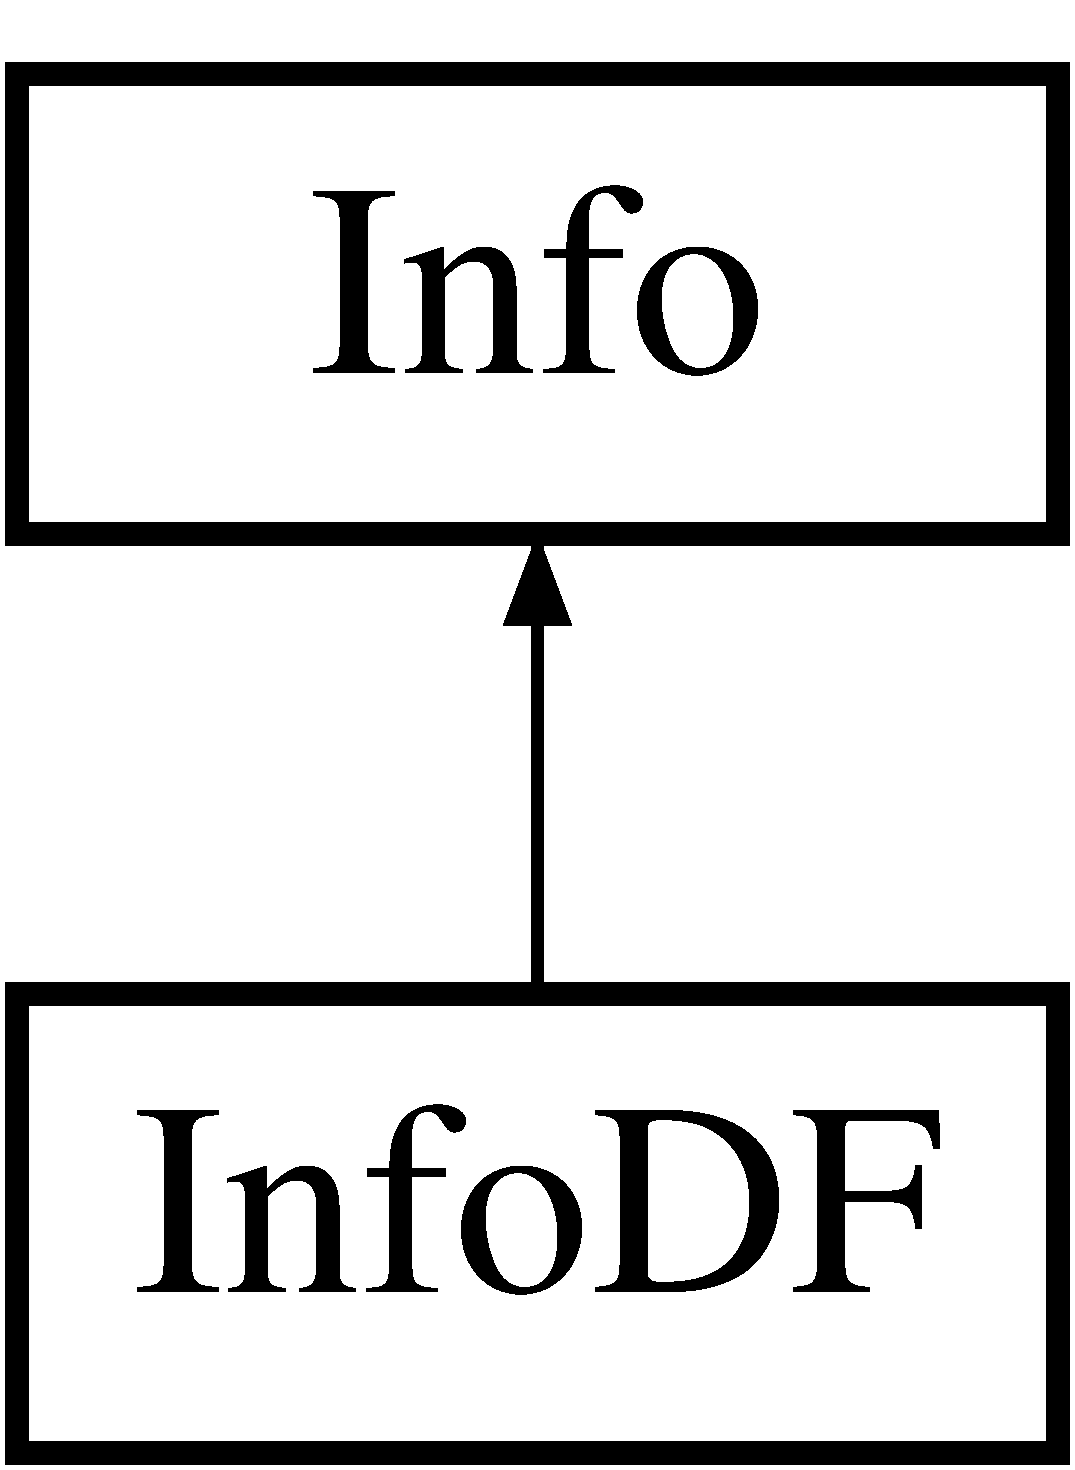
\includegraphics[height=2.000000cm]{class_info_d_f}
\end{center}
\end{figure}
\subsection*{Public Member Functions}
\begin{DoxyCompactItemize}
\item 
\hyperlink{class_info_d_f_af55f2bb64e046196f749756e4d5f8112}{Info\+DF} (\hyperlink{class_fraction}{Fraction} \hyperlink{class_info_ae893be5aad319de5d911c3f80cc0a2d4}{training\+Freq}, unsigned int \hyperlink{class_info_aabdfdb282f3ceaae1772574bf2b3cd86}{yellow\+Cards}, unsigned int \hyperlink{class_info_a953c30accc7e6ff301542adfd5824f38}{red\+Cards}, unsigned int \hyperlink{class_info_aecdd57d96490b16a0c2590dd8f34009e}{tackles}, unsigned int \hyperlink{class_info_a2f90c84ba67c0e225dd58cdc14ab7f3d}{fouls}, unsigned int \hyperlink{class_info_a5ad5f72833856502b9c1f6ea50a98619}{goals\+Scored}, unsigned int \hyperlink{class_info_a1c0340af11df3407946b0ffdaae28864}{assists}, \hyperlink{class_fraction}{Fraction} \hyperlink{class_info_a37ee53dc8ae9a9656206e7eb389c6392}{pass\+Accuracy}, vector$<$ \hyperlink{_utils_8hpp_a94ee089ecd5db12c81c7edbefaabff4d}{Defender\+Position} $>$ \hyperlink{class_info_d_f_ae694b60f6efc0190b16a99748b0eca40}{positions})
\begin{DoxyCompactList}\small\item\em \hyperlink{class_info_d_f}{Info\+DF}\textquotesingle{}s constructors. \end{DoxyCompactList}\item 
\hyperlink{class_info_d_f_abc2533cd09063a1bd3c70c82ab1a4f70}{Info\+DF} (string \&new\+Info)
\begin{DoxyCompactList}\small\item\em Constructor that creates new defender\textquotesingle{}s performance information by reading it from athletes file using a string. \end{DoxyCompactList}\item 
\hyperlink{class_info_d_f_a4643516a0a0ba1b391ff35f6267abdf2}{Info\+DF} ()
\begin{DoxyCompactList}\small\item\em Default constructor. \end{DoxyCompactList}\item 
\hyperlink{class_info_d_f_a54560987e55966335300ba6a3034c926}{Info\+DF} (istream \&in\+Stream)
\begin{DoxyCompactList}\small\item\em Constructor that creates new defender\textquotesingle{}s performance information by reading it from thae athletes file using a stringstream. \end{DoxyCompactList}\item 
vector$<$ \hyperlink{_utils_8hpp_a94ee089ecd5db12c81c7edbefaabff4d}{Defender\+Position} $>$ \hyperlink{class_info_d_f_a8e30128320b378b09477070781f9fe98}{get\+Defender\+Specific\+Positions} () const
\begin{DoxyCompactList}\small\item\em Gets the vector containing defender specific positions. \end{DoxyCompactList}\item 
void \hyperlink{class_info_d_f_aaa161b2c4a56878d3c691ec4de3129c3}{add\+Defender\+Specific\+Position} (\hyperlink{_utils_8hpp_a94ee089ecd5db12c81c7edbefaabff4d}{Defender\+Position} new\+Pos)
\begin{DoxyCompactList}\small\item\em Adds a defender specific position to the vector containing the different positions of the defender. \end{DoxyCompactList}\item 
string \hyperlink{class_info_d_f_a036c0f0898331e092f913da788b7ccdb}{generate\+String} () const
\begin{DoxyCompactList}\small\item\em Generates a string containing the defender\textquotesingle{}s performance information. \end{DoxyCompactList}\item 
void \hyperlink{class_info_d_f_a7dc54a1e9dbb5028eb1f9972d1e42951}{operator+=} (const \hyperlink{class_info}{Info} $\ast$info2)
\begin{DoxyCompactList}\small\item\em Addition assignment operator that adds two different blocks of defender\textquotesingle{}s performance information. \end{DoxyCompactList}\end{DoxyCompactItemize}
\subsection*{Protected Attributes}
\begin{DoxyCompactItemize}
\item 
vector$<$ \hyperlink{_utils_8hpp_a94ee089ecd5db12c81c7edbefaabff4d}{Defender\+Position} $>$ \hyperlink{class_info_d_f_ae694b60f6efc0190b16a99748b0eca40}{positions}
\begin{DoxyCompactList}\small\item\em vector containing the different defender positions. \end{DoxyCompactList}\end{DoxyCompactItemize}


\subsection{Detailed Description}
\hyperlink{class_defender}{Defender}\textquotesingle{}s performance information. 

Luís, 20/11/2016. 

\subsection{Constructor \& Destructor Documentation}
\hypertarget{class_info_d_f_af55f2bb64e046196f749756e4d5f8112}{}\label{class_info_d_f_af55f2bb64e046196f749756e4d5f8112} 
\index{Info\+DF@{Info\+DF}!Info\+DF@{Info\+DF}}
\index{Info\+DF@{Info\+DF}!Info\+DF@{Info\+DF}}
\subsubsection{\texorpdfstring{Info\+D\+F()}{InfoDF()}\hspace{0.1cm}{\footnotesize\ttfamily [1/4]}}
{\footnotesize\ttfamily Info\+D\+F\+::\+Info\+DF (\begin{DoxyParamCaption}\item[{\hyperlink{class_fraction}{Fraction}}]{training\+Freq,  }\item[{unsigned int}]{yellow\+Cards,  }\item[{unsigned int}]{red\+Cards,  }\item[{unsigned int}]{tackles,  }\item[{unsigned int}]{fouls,  }\item[{unsigned int}]{goals\+Scored,  }\item[{unsigned int}]{assists,  }\item[{\hyperlink{class_fraction}{Fraction}}]{pass\+Accuracy,  }\item[{vector$<$ \hyperlink{_utils_8hpp_a94ee089ecd5db12c81c7edbefaabff4d}{Defender\+Position} $>$}]{positions }\end{DoxyParamCaption})}



\hyperlink{class_info_d_f}{Info\+DF}\textquotesingle{}s constructors. 

This is a constructor that creates new defender\textquotesingle{}s performance information using training frequency, number of yellow cards, number of red cards, number of tackles, number of fouls commited, number of goals scored, number of assists, pass accuracy 

Constructor. 

Luís, 20/11/2016. 


\begin{DoxyParams}{Parameters}
{\em training\+Freq} & The training frequency. \\
\hline
{\em yellow\+Cards} & The yellow cards. \\
\hline
{\em red\+Cards} & The red cards. \\
\hline
{\em tackles} & The tackles. \\
\hline
{\em fouls} & The fouls. \\
\hline
{\em goals\+Scored} & The goals scored. \\
\hline
{\em assists} & The assists. \\
\hline
{\em pass\+Accuracy} & The pass accuracy. \\
\hline
{\em positions} & The positions. \\
\hline
\end{DoxyParams}
\hypertarget{class_info_d_f_abc2533cd09063a1bd3c70c82ab1a4f70}{}\label{class_info_d_f_abc2533cd09063a1bd3c70c82ab1a4f70} 
\index{Info\+DF@{Info\+DF}!Info\+DF@{Info\+DF}}
\index{Info\+DF@{Info\+DF}!Info\+DF@{Info\+DF}}
\subsubsection{\texorpdfstring{Info\+D\+F()}{InfoDF()}\hspace{0.1cm}{\footnotesize\ttfamily [2/4]}}
{\footnotesize\ttfamily Info\+D\+F\+::\+Info\+DF (\begin{DoxyParamCaption}\item[{string \&}]{new\+Info }\end{DoxyParamCaption})}



Constructor that creates new defender\textquotesingle{}s performance information by reading it from athletes file using a string. 

This is a constructor that creates new defender\textquotesingle{}s performance information by reading it from athletes file using a string

Luís, 20/11/2016. 


\begin{DoxyParams}{Parameters}
{\em new\+Info} & \mbox{[}in,out\mbox{]} Information describing the new. \\
\hline
\end{DoxyParams}
\hypertarget{class_info_d_f_a4643516a0a0ba1b391ff35f6267abdf2}{}\label{class_info_d_f_a4643516a0a0ba1b391ff35f6267abdf2} 
\index{Info\+DF@{Info\+DF}!Info\+DF@{Info\+DF}}
\index{Info\+DF@{Info\+DF}!Info\+DF@{Info\+DF}}
\subsubsection{\texorpdfstring{Info\+D\+F()}{InfoDF()}\hspace{0.1cm}{\footnotesize\ttfamily [3/4]}}
{\footnotesize\ttfamily Info\+D\+F\+::\+Info\+DF (\begin{DoxyParamCaption}{ }\end{DoxyParamCaption})}



Default constructor. 

This is the \hyperlink{class_info_d_f}{Info\+DF}\textquotesingle{}s class empty constructor

Luís, 20/11/2016. \hypertarget{class_info_d_f_a54560987e55966335300ba6a3034c926}{}\label{class_info_d_f_a54560987e55966335300ba6a3034c926} 
\index{Info\+DF@{Info\+DF}!Info\+DF@{Info\+DF}}
\index{Info\+DF@{Info\+DF}!Info\+DF@{Info\+DF}}
\subsubsection{\texorpdfstring{Info\+D\+F()}{InfoDF()}\hspace{0.1cm}{\footnotesize\ttfamily [4/4]}}
{\footnotesize\ttfamily Info\+D\+F\+::\+Info\+DF (\begin{DoxyParamCaption}\item[{istream \&}]{in\+Stream }\end{DoxyParamCaption})}



Constructor that creates new defender\textquotesingle{}s performance information by reading it from thae athletes file using a stringstream. 

This is a constructor that creates new defender\textquotesingle{}s performance information by reading it from thae athletes file using a stringstream

Luís, 20/11/2016. 


\begin{DoxyParams}{Parameters}
{\em in\+Stream} & \mbox{[}in,out\mbox{]} Stream to read data from. \\
\hline
\end{DoxyParams}


\subsection{Member Function Documentation}
\hypertarget{class_info_d_f_aaa161b2c4a56878d3c691ec4de3129c3}{}\label{class_info_d_f_aaa161b2c4a56878d3c691ec4de3129c3} 
\index{Info\+DF@{Info\+DF}!add\+Defender\+Specific\+Position@{add\+Defender\+Specific\+Position}}
\index{add\+Defender\+Specific\+Position@{add\+Defender\+Specific\+Position}!Info\+DF@{Info\+DF}}
\subsubsection{\texorpdfstring{add\+Defender\+Specific\+Position()}{addDefenderSpecificPosition()}}
{\footnotesize\ttfamily void Info\+D\+F\+::add\+Defender\+Specific\+Position (\begin{DoxyParamCaption}\item[{\hyperlink{_utils_8hpp_a94ee089ecd5db12c81c7edbefaabff4d}{Defender\+Position}}]{new\+Pos }\end{DoxyParamCaption})\hspace{0.3cm}{\ttfamily [virtual]}}



Adds a defender specific position to the vector containing the different positions of the defender. 

This is a method that adds a specific defender position to the vector containing the different positions of the defender

Luís, 20/11/2016. 


\begin{DoxyParams}{Parameters}
{\em new\+Pos} & The new position. \\
\hline
\end{DoxyParams}


Reimplemented from \hyperlink{class_info_a33d98f07e5a276f9a3d0a08275f559b3}{Info}.

\hypertarget{class_info_d_f_a036c0f0898331e092f913da788b7ccdb}{}\label{class_info_d_f_a036c0f0898331e092f913da788b7ccdb} 
\index{Info\+DF@{Info\+DF}!generate\+String@{generate\+String}}
\index{generate\+String@{generate\+String}!Info\+DF@{Info\+DF}}
\subsubsection{\texorpdfstring{generate\+String()}{generateString()}}
{\footnotesize\ttfamily string Info\+D\+F\+::generate\+String (\begin{DoxyParamCaption}{ }\end{DoxyParamCaption}) const\hspace{0.3cm}{\ttfamily [virtual]}}



Generates a string containing the defender\textquotesingle{}s performance information. 

This is a method that generates a string containing the defender\textquotesingle{}s performance information

Luís, 20/11/2016. 

\begin{DoxyReturn}{Returns}
The string containing the defender\textquotesingle{}s performance information. 
\end{DoxyReturn}


Reimplemented from \hyperlink{class_info_a5e52b35a9c17b58222bb57af16c16ce3}{Info}.

\hypertarget{class_info_d_f_a8e30128320b378b09477070781f9fe98}{}\label{class_info_d_f_a8e30128320b378b09477070781f9fe98} 
\index{Info\+DF@{Info\+DF}!get\+Defender\+Specific\+Positions@{get\+Defender\+Specific\+Positions}}
\index{get\+Defender\+Specific\+Positions@{get\+Defender\+Specific\+Positions}!Info\+DF@{Info\+DF}}
\subsubsection{\texorpdfstring{get\+Defender\+Specific\+Positions()}{getDefenderSpecificPositions()}}
{\footnotesize\ttfamily vector$<$ \hyperlink{_utils_8hpp_a94ee089ecd5db12c81c7edbefaabff4d}{Defender\+Position} $>$ Info\+D\+F\+::get\+Defender\+Specific\+Positions (\begin{DoxyParamCaption}{ }\end{DoxyParamCaption}) const\hspace{0.3cm}{\ttfamily [virtual]}}



Gets the vector containing defender specific positions. 

This is a method that gets the vector containing the different positions of the defender

Luís, 20/11/2016. 

\begin{DoxyReturn}{Returns}
The the vector containing defender specific positions. 
\end{DoxyReturn}


Reimplemented from \hyperlink{class_info_afa64d6a602f80674209e3391bf5fa309}{Info}.

\hypertarget{class_info_d_f_a7dc54a1e9dbb5028eb1f9972d1e42951}{}\label{class_info_d_f_a7dc54a1e9dbb5028eb1f9972d1e42951} 
\index{Info\+DF@{Info\+DF}!operator+=@{operator+=}}
\index{operator+=@{operator+=}!Info\+DF@{Info\+DF}}
\subsubsection{\texorpdfstring{operator+=()}{operator+=()}}
{\footnotesize\ttfamily void Info\+D\+F\+::operator+= (\begin{DoxyParamCaption}\item[{const \hyperlink{class_info}{Info} $\ast$}]{info2 }\end{DoxyParamCaption})\hspace{0.3cm}{\ttfamily [virtual]}}



Addition assignment operator that adds two different blocks of defender\textquotesingle{}s performance information. 

This is an assignment operator that adds two different blocks of defender\textquotesingle{}s performance information

Luís, 20/11/2016. 


\begin{DoxyParams}{Parameters}
{\em info2} & The second block information. \\
\hline
\end{DoxyParams}


Reimplemented from \hyperlink{class_info_a35d820d35f8ab3b8de15cdfc07f0c5a4}{Info}.



\subsection{Member Data Documentation}
\hypertarget{class_info_d_f_ae694b60f6efc0190b16a99748b0eca40}{}\label{class_info_d_f_ae694b60f6efc0190b16a99748b0eca40} 
\index{Info\+DF@{Info\+DF}!positions@{positions}}
\index{positions@{positions}!Info\+DF@{Info\+DF}}
\subsubsection{\texorpdfstring{positions}{positions}}
{\footnotesize\ttfamily vector$<$\hyperlink{_utils_8hpp_a94ee089ecd5db12c81c7edbefaabff4d}{Defender\+Position}$>$ Info\+D\+F\+::positions\hspace{0.3cm}{\ttfamily [protected]}}



vector containing the different defender positions. 



The documentation for this class was generated from the following files\+:\begin{DoxyCompactItemize}
\item 
\hyperlink{_info_athletes_8hpp}{Info\+Athletes.\+hpp}\item 
\hyperlink{_info_athletes_8cpp}{Info\+Athletes.\+cpp}\end{DoxyCompactItemize}

\hypertarget{class_info_f_w}{}\section{Info\+FW Class Reference}
\label{class_info_f_w}\index{Info\+FW@{Info\+FW}}


\hyperlink{class_forward}{Forward}\textquotesingle{}s performance information.  




{\ttfamily \#include $<$Info\+Athletes.\+hpp$>$}

Inheritance diagram for Info\+FW\+:\begin{figure}[H]
\begin{center}
\leavevmode
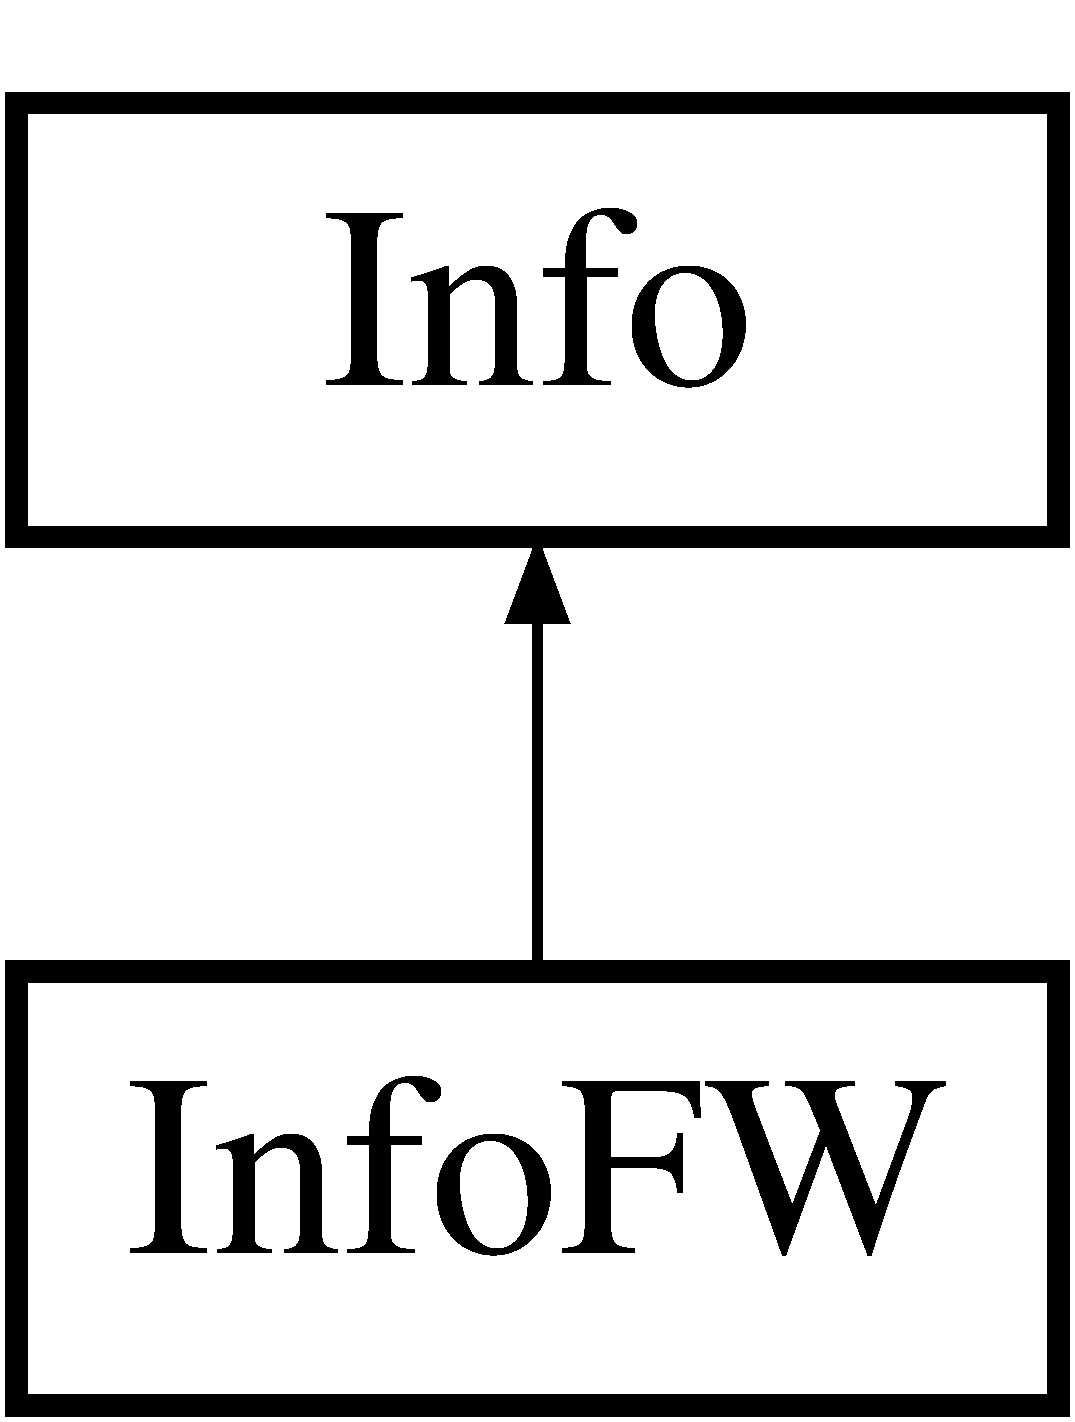
\includegraphics[height=2.000000cm]{class_info_f_w}
\end{center}
\end{figure}
\subsection*{Public Member Functions}
\begin{DoxyCompactItemize}
\item 
\hyperlink{class_info_f_w_a03c85ce3609ac34d37f0afee1e4a67c6}{Info\+FW} (\hyperlink{class_fraction}{Fraction} \hyperlink{class_info_ae893be5aad319de5d911c3f80cc0a2d4}{training\+Freq}, unsigned int \hyperlink{class_info_aabdfdb282f3ceaae1772574bf2b3cd86}{yellow\+Cards}, unsigned int \hyperlink{class_info_a953c30accc7e6ff301542adfd5824f38}{red\+Cards}, unsigned int \hyperlink{class_info_aecdd57d96490b16a0c2590dd8f34009e}{tackles}, unsigned int \hyperlink{class_info_a2f90c84ba67c0e225dd58cdc14ab7f3d}{fouls}, unsigned int \hyperlink{class_info_a5ad5f72833856502b9c1f6ea50a98619}{goals\+Scored}, unsigned int \hyperlink{class_info_a1c0340af11df3407946b0ffdaae28864}{assists}, \hyperlink{class_fraction}{Fraction} \hyperlink{class_info_a37ee53dc8ae9a9656206e7eb389c6392}{pass\+Accuracy}, vector$<$ \hyperlink{_utils_8hpp_ae6ffae6f01bd3312aac4a44642f14620}{Forward\+Position} $>$ \hyperlink{class_info_f_w_ab6a247d57fee089e4a7ad08e798c101b}{positions})
\begin{DoxyCompactList}\small\item\em \hyperlink{class_info_f_w}{Info\+FW}\textquotesingle{}s constructors. \end{DoxyCompactList}\item 
\hyperlink{class_info_f_w_ad4b4d077d84d8943bb1bccf8a9679e63}{Info\+FW} (string \&new\+Info)
\begin{DoxyCompactList}\small\item\em Constructor that creates new forward\textquotesingle{}s performance information by reading it from athletes file using a string. \end{DoxyCompactList}\item 
\hyperlink{class_info_f_w_aa45a6024762145dffd2c6c82648bc2ea}{Info\+FW} ()
\begin{DoxyCompactList}\small\item\em Default constructor. \end{DoxyCompactList}\item 
\hyperlink{class_info_f_w_a2d29763451213dd0f92fee314e3ff2e9}{Info\+FW} (istream \&in\+Stream)
\begin{DoxyCompactList}\small\item\em Constructor that creates new forward\textquotesingle{}s performance information by reading it from thae athletes file using a stringstream. \end{DoxyCompactList}\item 
vector$<$ \hyperlink{_utils_8hpp_ae6ffae6f01bd3312aac4a44642f14620}{Forward\+Position} $>$ \hyperlink{class_info_f_w_a9bce628dbf938dc530f9333d587b100a}{get\+Forward\+Specific\+Positions} () const
\begin{DoxyCompactList}\small\item\em Gets the vector containing forward specific positions. \end{DoxyCompactList}\item 
void \hyperlink{class_info_f_w_af8af688ba3e796239736dd9ce450991f}{add\+Attacker\+Specific\+Position} (\hyperlink{_utils_8hpp_ae6ffae6f01bd3312aac4a44642f14620}{Forward\+Position} new\+Pos)
\begin{DoxyCompactList}\small\item\em Adds an attacker specific position to the vector containing the different positions of the forward. \end{DoxyCompactList}\item 
string \hyperlink{class_info_f_w_a4c5957205aa850fcdc1d6ba30f085543}{generate\+String} () const
\begin{DoxyCompactList}\small\item\em Generates a string containing the forward\textquotesingle{}s performance information. \end{DoxyCompactList}\item 
void \hyperlink{class_info_f_w_aa4819d4c6348908eee81e5e71552cf8d}{operator+=} (const \hyperlink{class_info}{Info} $\ast$info2)
\begin{DoxyCompactList}\small\item\em Addition assignment operator that adds two different blocks of forward\textquotesingle{}s performance information. \end{DoxyCompactList}\end{DoxyCompactItemize}
\subsection*{Protected Attributes}
\begin{DoxyCompactItemize}
\item 
vector$<$ \hyperlink{_utils_8hpp_ae6ffae6f01bd3312aac4a44642f14620}{Forward\+Position} $>$ \hyperlink{class_info_f_w_ab6a247d57fee089e4a7ad08e798c101b}{positions}
\begin{DoxyCompactList}\small\item\em vector containing the different midfielder positions. \end{DoxyCompactList}\end{DoxyCompactItemize}


\subsection{Detailed Description}
\hyperlink{class_forward}{Forward}\textquotesingle{}s performance information. 

Luís, 20/11/2016. 

\subsection{Constructor \& Destructor Documentation}
\hypertarget{class_info_f_w_a03c85ce3609ac34d37f0afee1e4a67c6}{}\label{class_info_f_w_a03c85ce3609ac34d37f0afee1e4a67c6} 
\index{Info\+FW@{Info\+FW}!Info\+FW@{Info\+FW}}
\index{Info\+FW@{Info\+FW}!Info\+FW@{Info\+FW}}
\subsubsection{\texorpdfstring{Info\+F\+W()}{InfoFW()}\hspace{0.1cm}{\footnotesize\ttfamily [1/4]}}
{\footnotesize\ttfamily Info\+F\+W\+::\+Info\+FW (\begin{DoxyParamCaption}\item[{\hyperlink{class_fraction}{Fraction}}]{training\+Freq,  }\item[{unsigned int}]{yellow\+Cards,  }\item[{unsigned int}]{red\+Cards,  }\item[{unsigned int}]{tackles,  }\item[{unsigned int}]{fouls,  }\item[{unsigned int}]{goals\+Scored,  }\item[{unsigned int}]{assists,  }\item[{\hyperlink{class_fraction}{Fraction}}]{pass\+Accuracy,  }\item[{vector$<$ \hyperlink{_utils_8hpp_ae6ffae6f01bd3312aac4a44642f14620}{Forward\+Position} $>$}]{positions }\end{DoxyParamCaption})}



\hyperlink{class_info_f_w}{Info\+FW}\textquotesingle{}s constructors. 

This is a constructor that creates new forward\textquotesingle{}s performance information using training frequency, number of yellow cards, number of red cards, number of tackles, number of fouls commited, number of goals scored, number of assists, pass accuracy 

Constructor. 

Luís, 20/11/2016. 


\begin{DoxyParams}{Parameters}
{\em training\+Freq} & The training frequency. \\
\hline
{\em yellow\+Cards} & The yellow cards. \\
\hline
{\em red\+Cards} & The red cards. \\
\hline
{\em tackles} & The tackles. \\
\hline
{\em fouls} & The fouls. \\
\hline
{\em goals\+Scored} & The goals scored. \\
\hline
{\em assists} & The assists. \\
\hline
{\em pass\+Accuracy} & The pass accuracy. \\
\hline
{\em positions} & The positions. \\
\hline
\end{DoxyParams}
\hypertarget{class_info_f_w_ad4b4d077d84d8943bb1bccf8a9679e63}{}\label{class_info_f_w_ad4b4d077d84d8943bb1bccf8a9679e63} 
\index{Info\+FW@{Info\+FW}!Info\+FW@{Info\+FW}}
\index{Info\+FW@{Info\+FW}!Info\+FW@{Info\+FW}}
\subsubsection{\texorpdfstring{Info\+F\+W()}{InfoFW()}\hspace{0.1cm}{\footnotesize\ttfamily [2/4]}}
{\footnotesize\ttfamily Info\+F\+W\+::\+Info\+FW (\begin{DoxyParamCaption}\item[{string \&}]{new\+Info }\end{DoxyParamCaption})}



Constructor that creates new forward\textquotesingle{}s performance information by reading it from athletes file using a string. 

This is a constructor that creates new forward\textquotesingle{}s performance information by reading it from athletes file using a string

Luís, 20/11/2016. 


\begin{DoxyParams}{Parameters}
{\em new\+Info} & \mbox{[}in,out\mbox{]} Information describing the new. \\
\hline
\end{DoxyParams}
\hypertarget{class_info_f_w_aa45a6024762145dffd2c6c82648bc2ea}{}\label{class_info_f_w_aa45a6024762145dffd2c6c82648bc2ea} 
\index{Info\+FW@{Info\+FW}!Info\+FW@{Info\+FW}}
\index{Info\+FW@{Info\+FW}!Info\+FW@{Info\+FW}}
\subsubsection{\texorpdfstring{Info\+F\+W()}{InfoFW()}\hspace{0.1cm}{\footnotesize\ttfamily [3/4]}}
{\footnotesize\ttfamily Info\+F\+W\+::\+Info\+FW (\begin{DoxyParamCaption}{ }\end{DoxyParamCaption})}



Default constructor. 

This is the \hyperlink{class_info_f_w}{Info\+FW}\textquotesingle{}s class empty constructor

Luís, 20/11/2016. \hypertarget{class_info_f_w_a2d29763451213dd0f92fee314e3ff2e9}{}\label{class_info_f_w_a2d29763451213dd0f92fee314e3ff2e9} 
\index{Info\+FW@{Info\+FW}!Info\+FW@{Info\+FW}}
\index{Info\+FW@{Info\+FW}!Info\+FW@{Info\+FW}}
\subsubsection{\texorpdfstring{Info\+F\+W()}{InfoFW()}\hspace{0.1cm}{\footnotesize\ttfamily [4/4]}}
{\footnotesize\ttfamily Info\+F\+W\+::\+Info\+FW (\begin{DoxyParamCaption}\item[{istream \&}]{in\+Stream }\end{DoxyParamCaption})}



Constructor that creates new forward\textquotesingle{}s performance information by reading it from thae athletes file using a stringstream. 

This is a constructor that creates new forward\textquotesingle{}s performance information by reading it from thae athletes file using a stringstream

Luís, 20/11/2016. 


\begin{DoxyParams}{Parameters}
{\em in\+Stream} & \mbox{[}in,out\mbox{]} Stream to read data from. \\
\hline
\end{DoxyParams}


\subsection{Member Function Documentation}
\hypertarget{class_info_f_w_af8af688ba3e796239736dd9ce450991f}{}\label{class_info_f_w_af8af688ba3e796239736dd9ce450991f} 
\index{Info\+FW@{Info\+FW}!add\+Attacker\+Specific\+Position@{add\+Attacker\+Specific\+Position}}
\index{add\+Attacker\+Specific\+Position@{add\+Attacker\+Specific\+Position}!Info\+FW@{Info\+FW}}
\subsubsection{\texorpdfstring{add\+Attacker\+Specific\+Position()}{addAttackerSpecificPosition()}}
{\footnotesize\ttfamily void Info\+F\+W\+::add\+Attacker\+Specific\+Position (\begin{DoxyParamCaption}\item[{\hyperlink{_utils_8hpp_ae6ffae6f01bd3312aac4a44642f14620}{Forward\+Position}}]{new\+Pos }\end{DoxyParamCaption})\hspace{0.3cm}{\ttfamily [virtual]}}



Adds an attacker specific position to the vector containing the different positions of the forward. 

This is a method that adds a specific forward position to the vector containing the different positions of the forward

Luís, 20/11/2016. 


\begin{DoxyParams}{Parameters}
{\em new\+Pos} & The new position. \\
\hline
\end{DoxyParams}


Reimplemented from \hyperlink{class_info_afba094a1c19e8ff4bb3a9048ca6c7f4a}{Info}.

\hypertarget{class_info_f_w_a4c5957205aa850fcdc1d6ba30f085543}{}\label{class_info_f_w_a4c5957205aa850fcdc1d6ba30f085543} 
\index{Info\+FW@{Info\+FW}!generate\+String@{generate\+String}}
\index{generate\+String@{generate\+String}!Info\+FW@{Info\+FW}}
\subsubsection{\texorpdfstring{generate\+String()}{generateString()}}
{\footnotesize\ttfamily string Info\+F\+W\+::generate\+String (\begin{DoxyParamCaption}{ }\end{DoxyParamCaption}) const\hspace{0.3cm}{\ttfamily [virtual]}}



Generates a string containing the forward\textquotesingle{}s performance information. 

This is a method that generates a string containing the forward\textquotesingle{}s performance information

Luís, 20/11/2016. 

\begin{DoxyReturn}{Returns}
The string containing the forward\textquotesingle{}s performance information. 
\end{DoxyReturn}


Reimplemented from \hyperlink{class_info_a5e52b35a9c17b58222bb57af16c16ce3}{Info}.

\hypertarget{class_info_f_w_a9bce628dbf938dc530f9333d587b100a}{}\label{class_info_f_w_a9bce628dbf938dc530f9333d587b100a} 
\index{Info\+FW@{Info\+FW}!get\+Forward\+Specific\+Positions@{get\+Forward\+Specific\+Positions}}
\index{get\+Forward\+Specific\+Positions@{get\+Forward\+Specific\+Positions}!Info\+FW@{Info\+FW}}
\subsubsection{\texorpdfstring{get\+Forward\+Specific\+Positions()}{getForwardSpecificPositions()}}
{\footnotesize\ttfamily vector$<$ \hyperlink{_utils_8hpp_ae6ffae6f01bd3312aac4a44642f14620}{Forward\+Position} $>$ Info\+F\+W\+::get\+Forward\+Specific\+Positions (\begin{DoxyParamCaption}{ }\end{DoxyParamCaption}) const\hspace{0.3cm}{\ttfamily [virtual]}}



Gets the vector containing forward specific positions. 

This is a method that gets the vector containing the different positions of the forward

Luís, 20/11/2016. 

\begin{DoxyReturn}{Returns}
The vector containing forward specific positions. 
\end{DoxyReturn}


Reimplemented from \hyperlink{class_info_abff2f6cd7a845b8bd80c97d9d456e07e}{Info}.

\hypertarget{class_info_f_w_aa4819d4c6348908eee81e5e71552cf8d}{}\label{class_info_f_w_aa4819d4c6348908eee81e5e71552cf8d} 
\index{Info\+FW@{Info\+FW}!operator+=@{operator+=}}
\index{operator+=@{operator+=}!Info\+FW@{Info\+FW}}
\subsubsection{\texorpdfstring{operator+=()}{operator+=()}}
{\footnotesize\ttfamily void Info\+F\+W\+::operator+= (\begin{DoxyParamCaption}\item[{const \hyperlink{class_info}{Info} $\ast$}]{info2 }\end{DoxyParamCaption})\hspace{0.3cm}{\ttfamily [virtual]}}



Addition assignment operator that adds two different blocks of forward\textquotesingle{}s performance information. 

This is an assignment operator that adds two different blocks of forward\textquotesingle{}s performance information

Luís, 20/11/2016. 


\begin{DoxyParams}{Parameters}
{\em info2} & The second block information. \\
\hline
\end{DoxyParams}


Reimplemented from \hyperlink{class_info_a35d820d35f8ab3b8de15cdfc07f0c5a4}{Info}.



\subsection{Member Data Documentation}
\hypertarget{class_info_f_w_ab6a247d57fee089e4a7ad08e798c101b}{}\label{class_info_f_w_ab6a247d57fee089e4a7ad08e798c101b} 
\index{Info\+FW@{Info\+FW}!positions@{positions}}
\index{positions@{positions}!Info\+FW@{Info\+FW}}
\subsubsection{\texorpdfstring{positions}{positions}}
{\footnotesize\ttfamily vector$<$\hyperlink{_utils_8hpp_ae6ffae6f01bd3312aac4a44642f14620}{Forward\+Position}$>$ Info\+F\+W\+::positions\hspace{0.3cm}{\ttfamily [protected]}}



vector containing the different midfielder positions. 



The documentation for this class was generated from the following files\+:\begin{DoxyCompactItemize}
\item 
\hyperlink{_info_athletes_8hpp}{Info\+Athletes.\+hpp}\item 
\hyperlink{_info_athletes_8cpp}{Info\+Athletes.\+cpp}\end{DoxyCompactItemize}

\hypertarget{class_info_g_k}{}\section{Info\+GK Class Reference}
\label{class_info_g_k}\index{Info\+GK@{Info\+GK}}


{\ttfamily \#include $<$Info\+Athletes.\+hpp$>$}

Inheritance diagram for Info\+GK\+:\begin{figure}[H]
\begin{center}
\leavevmode
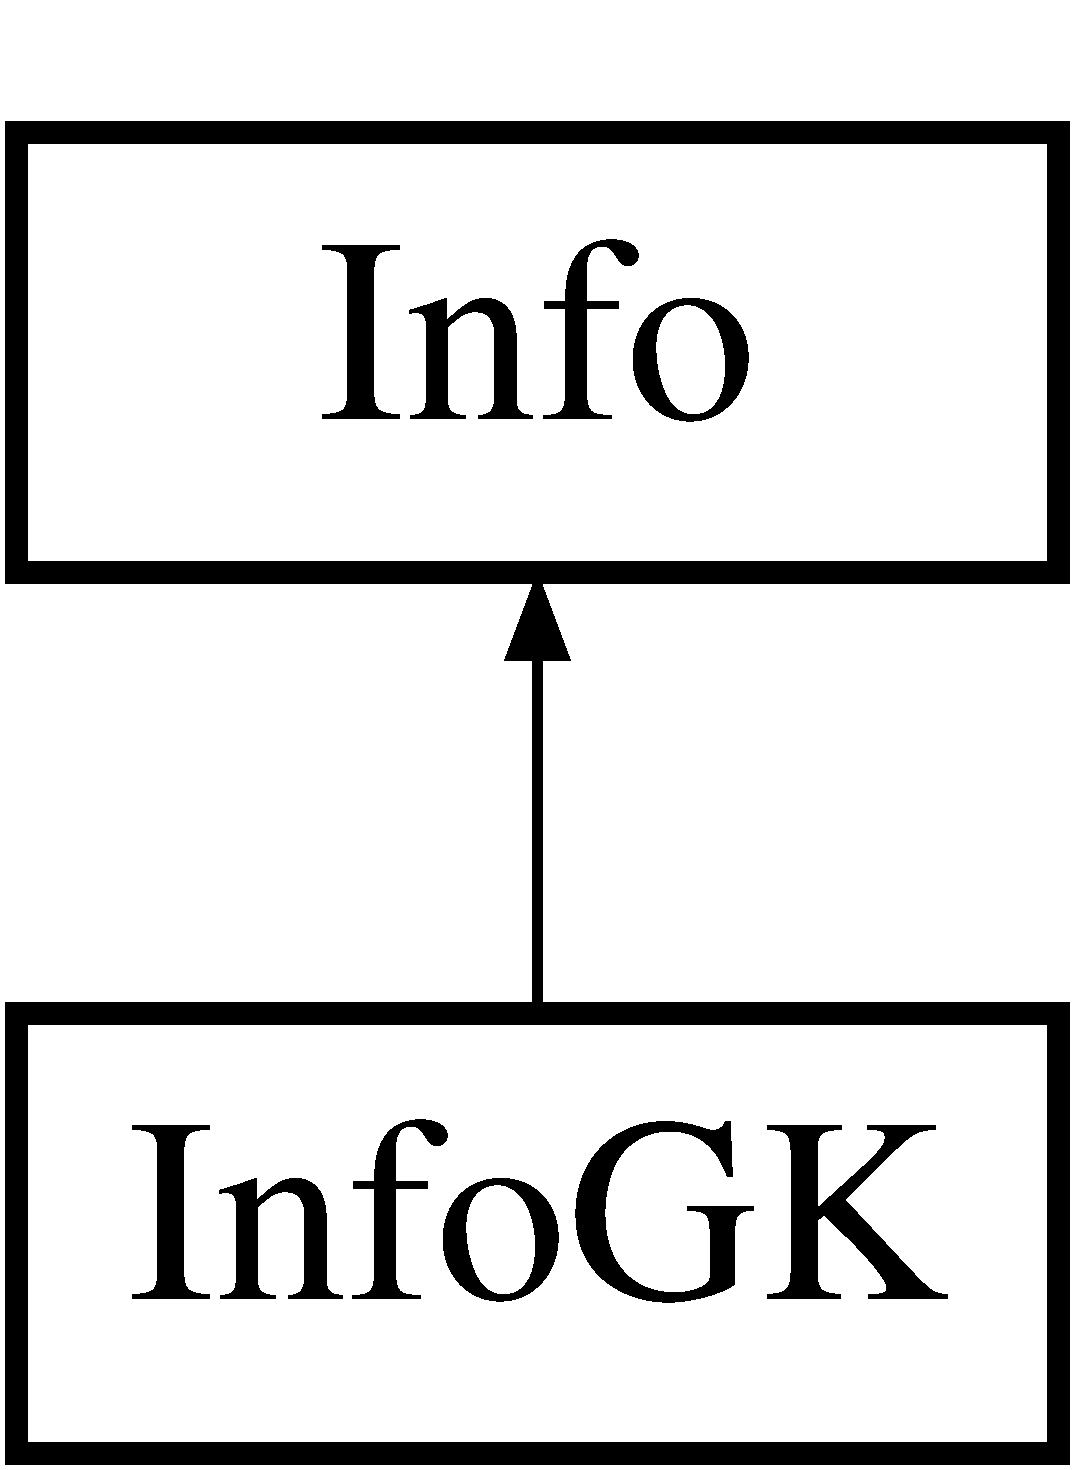
\includegraphics[height=2.000000cm]{class_info_g_k}
\end{center}
\end{figure}
\subsection*{Public Member Functions}
\begin{DoxyCompactItemize}
\item 
\hyperlink{class_info_g_k_ae71501a397ad142ce48e7136be6ebb06}{Info\+GK} (\hyperlink{class_fraction}{Fraction} \hyperlink{class_info_ae893be5aad319de5d911c3f80cc0a2d4}{training\+Freq}, unsigned int \hyperlink{class_info_aabdfdb282f3ceaae1772574bf2b3cd86}{yellow\+Cards}, unsigned int \hyperlink{class_info_a953c30accc7e6ff301542adfd5824f38}{red\+Cards}, unsigned int \hyperlink{class_info_aecdd57d96490b16a0c2590dd8f34009e}{tackles}, unsigned int \hyperlink{class_info_a2f90c84ba67c0e225dd58cdc14ab7f3d}{fouls}, unsigned int \hyperlink{class_info_a5ad5f72833856502b9c1f6ea50a98619}{goals\+Scored}, unsigned int \hyperlink{class_info_a1c0340af11df3407946b0ffdaae28864}{assists}, \hyperlink{class_fraction}{Fraction} \hyperlink{class_info_a37ee53dc8ae9a9656206e7eb389c6392}{pass\+Accuracy}, unsigned int \hyperlink{class_info_g_k_a0cd48fb9138effb26433639f12311794}{saves}, unsigned int \hyperlink{class_info_g_k_a1380b4f12dffe7a8cadd23e06e5c645f}{goals\+Conceeded})
\begin{DoxyCompactList}\small\item\em \hyperlink{class_info_g_k}{Info\+GK}\textquotesingle{}s constructors. \end{DoxyCompactList}\item 
\hyperlink{class_info_g_k_a3492995eb8a38acae93a8068a6be36ea}{Info\+GK} (string \&new\+Info)
\begin{DoxyCompactList}\small\item\em Constructor that creates new goalkeeper\textquotesingle{}s performance information by reading it from athletes file using a string. \end{DoxyCompactList}\item 
\hyperlink{class_info_g_k_a433a9a5bf75d9624be89100bc2e2e118}{Info\+GK} ()
\begin{DoxyCompactList}\small\item\em Default constructor. \end{DoxyCompactList}\item 
\hyperlink{class_info_g_k_aeace217be1619844c5637ba5cd3717ef}{Info\+GK} (istream \&in\+Stream)
\begin{DoxyCompactList}\small\item\em Constructor that creates new goalkeeper\textquotesingle{}s performance information by reading it from thae athletes file using a stringstream. \end{DoxyCompactList}\item 
unsigned int \hyperlink{class_info_g_k_a5690b8056b8f30b5127f99b46ef9a5d9}{get\+Saves} () const
\begin{DoxyCompactList}\small\item\em Gets the number of saves made by the goalkeeper. \end{DoxyCompactList}\item 
void \hyperlink{class_info_g_k_aa1535598fa29b199374a404dda8b73f2}{add\+Saves} (unsigned int \hyperlink{class_info_g_k_a0cd48fb9138effb26433639f12311794}{saves})
\begin{DoxyCompactList}\small\item\em Adds the saves to the total number of saves made by the goalkeeper. \end{DoxyCompactList}\item 
unsigned int \hyperlink{class_info_g_k_a069874de6c798b3237388f3dbdb14de1}{get\+Goals\+Conceeded} () const
\begin{DoxyCompactList}\small\item\em Gets the number of goals conceeded by the goalkeeper. \end{DoxyCompactList}\item 
void \hyperlink{class_info_g_k_aa29eeb0025487da9106007246478a0b5}{add\+Goals\+Conceeded} (unsigned int \hyperlink{class_info_g_k_a1380b4f12dffe7a8cadd23e06e5c645f}{goals\+Conceeded})
\begin{DoxyCompactList}\small\item\em Adds goals conceeded to total number of goals conceeded by the goalkeeper. \end{DoxyCompactList}\item 
string \hyperlink{class_info_g_k_a7bdc5a14f105385b4d856c8df7a4c7d0}{generate\+String} () const
\begin{DoxyCompactList}\small\item\em Generates a string containing the goalkeeper\textquotesingle{}s performance information. \end{DoxyCompactList}\item 
void \hyperlink{class_info_g_k_a1554aaf307cb45226fb26c6d6380a47e}{operator+=} (const \hyperlink{class_info}{Info} $\ast$info2)
\begin{DoxyCompactList}\small\item\em Addition assignment operator that adds two different blocks of goalkeeper\textquotesingle{}s performance information. \end{DoxyCompactList}\end{DoxyCompactItemize}
\subsection*{Protected Attributes}
\begin{DoxyCompactItemize}
\item 
unsigned int \hyperlink{class_info_g_k_a0cd48fb9138effb26433639f12311794}{saves}
\begin{DoxyCompactList}\small\item\em saves made by the goalkeeper atribute. \end{DoxyCompactList}\item 
unsigned int \hyperlink{class_info_g_k_a1380b4f12dffe7a8cadd23e06e5c645f}{goals\+Conceeded}
\begin{DoxyCompactList}\small\item\em goals conceeded by the goalkeeper atribute. \end{DoxyCompactList}\end{DoxyCompactItemize}


\subsection{Constructor \& Destructor Documentation}
\hypertarget{class_info_g_k_ae71501a397ad142ce48e7136be6ebb06}{}\label{class_info_g_k_ae71501a397ad142ce48e7136be6ebb06} 
\index{Info\+GK@{Info\+GK}!Info\+GK@{Info\+GK}}
\index{Info\+GK@{Info\+GK}!Info\+GK@{Info\+GK}}
\subsubsection{\texorpdfstring{Info\+G\+K()}{InfoGK()}\hspace{0.1cm}{\footnotesize\ttfamily [1/4]}}
{\footnotesize\ttfamily Info\+G\+K\+::\+Info\+GK (\begin{DoxyParamCaption}\item[{\hyperlink{class_fraction}{Fraction}}]{training\+Freq,  }\item[{unsigned int}]{yellow\+Cards,  }\item[{unsigned int}]{red\+Cards,  }\item[{unsigned int}]{tackles,  }\item[{unsigned int}]{fouls,  }\item[{unsigned int}]{goals\+Scored,  }\item[{unsigned int}]{assists,  }\item[{\hyperlink{class_fraction}{Fraction}}]{pass\+Accuracy,  }\item[{unsigned int}]{saves,  }\item[{unsigned int}]{goals\+Conceeded }\end{DoxyParamCaption})}



\hyperlink{class_info_g_k}{Info\+GK}\textquotesingle{}s constructors. 

This is a constructor that creates new goalkeeper\textquotesingle{}s performance information using training frequency, number of yellow cards, number of red cards, number of tackles, number of fouls commited, number of goals scored, number of assists, pass accuracy 

Constructor. 

Luís, 20/11/2016. 


\begin{DoxyParams}{Parameters}
{\em training\+Freq} & The training frequency. \\
\hline
{\em yellow\+Cards} & The yellow cards. \\
\hline
{\em red\+Cards} & The red cards. \\
\hline
{\em tackles} & The tackles. \\
\hline
{\em fouls} & The fouls. \\
\hline
{\em goals\+Scored} & The goals scored. \\
\hline
{\em assists} & The assists. \\
\hline
{\em pass\+Accuracy} & The pass accuracy. \\
\hline
{\em saves} & The saves. \\
\hline
{\em goals\+Conceeded} & The goals conceeded. \\
\hline
\end{DoxyParams}
\hypertarget{class_info_g_k_a3492995eb8a38acae93a8068a6be36ea}{}\label{class_info_g_k_a3492995eb8a38acae93a8068a6be36ea} 
\index{Info\+GK@{Info\+GK}!Info\+GK@{Info\+GK}}
\index{Info\+GK@{Info\+GK}!Info\+GK@{Info\+GK}}
\subsubsection{\texorpdfstring{Info\+G\+K()}{InfoGK()}\hspace{0.1cm}{\footnotesize\ttfamily [2/4]}}
{\footnotesize\ttfamily Info\+G\+K\+::\+Info\+GK (\begin{DoxyParamCaption}\item[{string \&}]{new\+Info }\end{DoxyParamCaption})}



Constructor that creates new goalkeeper\textquotesingle{}s performance information by reading it from athletes file using a string. 

This is a constructor that creates new goalkeeper\textquotesingle{}s performance information by reading it from athletes file using a string

Luís, 20/11/2016. 


\begin{DoxyParams}{Parameters}
{\em new\+Info} & \mbox{[}in,out\mbox{]} Information describing the new. \\
\hline
\end{DoxyParams}
\hypertarget{class_info_g_k_a433a9a5bf75d9624be89100bc2e2e118}{}\label{class_info_g_k_a433a9a5bf75d9624be89100bc2e2e118} 
\index{Info\+GK@{Info\+GK}!Info\+GK@{Info\+GK}}
\index{Info\+GK@{Info\+GK}!Info\+GK@{Info\+GK}}
\subsubsection{\texorpdfstring{Info\+G\+K()}{InfoGK()}\hspace{0.1cm}{\footnotesize\ttfamily [3/4]}}
{\footnotesize\ttfamily Info\+G\+K\+::\+Info\+GK (\begin{DoxyParamCaption}{ }\end{DoxyParamCaption})}



Default constructor. 

Luís, 20/11/2016. \hypertarget{class_info_g_k_aeace217be1619844c5637ba5cd3717ef}{}\label{class_info_g_k_aeace217be1619844c5637ba5cd3717ef} 
\index{Info\+GK@{Info\+GK}!Info\+GK@{Info\+GK}}
\index{Info\+GK@{Info\+GK}!Info\+GK@{Info\+GK}}
\subsubsection{\texorpdfstring{Info\+G\+K()}{InfoGK()}\hspace{0.1cm}{\footnotesize\ttfamily [4/4]}}
{\footnotesize\ttfamily Info\+G\+K\+::\+Info\+GK (\begin{DoxyParamCaption}\item[{istream \&}]{in\+Stream }\end{DoxyParamCaption})}



Constructor that creates new goalkeeper\textquotesingle{}s performance information by reading it from thae athletes file using a stringstream. 

Luís, 20/11/2016. 


\begin{DoxyParams}{Parameters}
{\em in\+Stream} & \mbox{[}in,out\mbox{]} Stream to read data from. \\
\hline
\end{DoxyParams}


\subsection{Member Function Documentation}
\hypertarget{class_info_g_k_aa29eeb0025487da9106007246478a0b5}{}\label{class_info_g_k_aa29eeb0025487da9106007246478a0b5} 
\index{Info\+GK@{Info\+GK}!add\+Goals\+Conceeded@{add\+Goals\+Conceeded}}
\index{add\+Goals\+Conceeded@{add\+Goals\+Conceeded}!Info\+GK@{Info\+GK}}
\subsubsection{\texorpdfstring{add\+Goals\+Conceeded()}{addGoalsConceeded()}}
{\footnotesize\ttfamily void Info\+G\+K\+::add\+Goals\+Conceeded (\begin{DoxyParamCaption}\item[{unsigned int}]{goals\+Conceeded }\end{DoxyParamCaption})\hspace{0.3cm}{\ttfamily [virtual]}}



Adds goals conceeded to total number of goals conceeded by the goalkeeper. 

This is a virtual method that adds goals conceeded to total number of goals conceeded by the goalkeeper

Luís, 20/11/2016. 


\begin{DoxyParams}{Parameters}
{\em goals\+Conceeded} & The goals conceeded. \\
\hline
\end{DoxyParams}


Reimplemented from \hyperlink{class_info_ae252f25a8dff58017b92ba7a5ad02bc0}{Info}.

\hypertarget{class_info_g_k_aa1535598fa29b199374a404dda8b73f2}{}\label{class_info_g_k_aa1535598fa29b199374a404dda8b73f2} 
\index{Info\+GK@{Info\+GK}!add\+Saves@{add\+Saves}}
\index{add\+Saves@{add\+Saves}!Info\+GK@{Info\+GK}}
\subsubsection{\texorpdfstring{add\+Saves()}{addSaves()}}
{\footnotesize\ttfamily void Info\+G\+K\+::add\+Saves (\begin{DoxyParamCaption}\item[{unsigned int}]{saves }\end{DoxyParamCaption})\hspace{0.3cm}{\ttfamily [virtual]}}



Adds the saves to the total number of saves made by the goalkeeper. 

This is a method that adds saves to the total number of saves made by the goalkeeper

Luís, 20/11/2016. 


\begin{DoxyParams}{Parameters}
{\em saves} & The saves. \\
\hline
\end{DoxyParams}


Reimplemented from \hyperlink{class_info_a7e66fc93d6ab97827bbf50fa61c71186}{Info}.

\hypertarget{class_info_g_k_a7bdc5a14f105385b4d856c8df7a4c7d0}{}\label{class_info_g_k_a7bdc5a14f105385b4d856c8df7a4c7d0} 
\index{Info\+GK@{Info\+GK}!generate\+String@{generate\+String}}
\index{generate\+String@{generate\+String}!Info\+GK@{Info\+GK}}
\subsubsection{\texorpdfstring{generate\+String()}{generateString()}}
{\footnotesize\ttfamily string Info\+G\+K\+::generate\+String (\begin{DoxyParamCaption}{ }\end{DoxyParamCaption}) const\hspace{0.3cm}{\ttfamily [virtual]}}



Generates a string containing the goalkeeper\textquotesingle{}s performance information. 

This is a method that generates a string containing the goalkeeper\textquotesingle{}s performance information

Luís, 20/11/2016. 

\begin{DoxyReturn}{Returns}
The string containing the goalkeeper\textquotesingle{}s performance information. 
\end{DoxyReturn}


Reimplemented from \hyperlink{class_info_a5e52b35a9c17b58222bb57af16c16ce3}{Info}.

\hypertarget{class_info_g_k_a069874de6c798b3237388f3dbdb14de1}{}\label{class_info_g_k_a069874de6c798b3237388f3dbdb14de1} 
\index{Info\+GK@{Info\+GK}!get\+Goals\+Conceeded@{get\+Goals\+Conceeded}}
\index{get\+Goals\+Conceeded@{get\+Goals\+Conceeded}!Info\+GK@{Info\+GK}}
\subsubsection{\texorpdfstring{get\+Goals\+Conceeded()}{getGoalsConceeded()}}
{\footnotesize\ttfamily unsigned int Info\+G\+K\+::get\+Goals\+Conceeded (\begin{DoxyParamCaption}{ }\end{DoxyParamCaption}) const\hspace{0.3cm}{\ttfamily [virtual]}}



Gets the number of goals conceeded by the goalkeeper. 

This is a method that gets the number of goals conceeded by the goalkeeper

Luís, 20/11/2016. 

\begin{DoxyReturn}{Returns}
The goals conceeded. 
\end{DoxyReturn}


Reimplemented from \hyperlink{class_info_a41d954fad291a5ffdfe29cb1cf3f75ce}{Info}.

\hypertarget{class_info_g_k_a5690b8056b8f30b5127f99b46ef9a5d9}{}\label{class_info_g_k_a5690b8056b8f30b5127f99b46ef9a5d9} 
\index{Info\+GK@{Info\+GK}!get\+Saves@{get\+Saves}}
\index{get\+Saves@{get\+Saves}!Info\+GK@{Info\+GK}}
\subsubsection{\texorpdfstring{get\+Saves()}{getSaves()}}
{\footnotesize\ttfamily unsigned int Info\+G\+K\+::get\+Saves (\begin{DoxyParamCaption}{ }\end{DoxyParamCaption}) const\hspace{0.3cm}{\ttfamily [virtual]}}



Gets the number of saves made by the goalkeeper. 

This is a method that adds saves to the total number of saves made by the goalkeeper

Luís, 20/11/2016. 

\begin{DoxyReturn}{Returns}
The saves. 
\end{DoxyReturn}


Reimplemented from \hyperlink{class_info_a2d7c53d322a705aaeb08fb79f9ef5211}{Info}.

\hypertarget{class_info_g_k_a1554aaf307cb45226fb26c6d6380a47e}{}\label{class_info_g_k_a1554aaf307cb45226fb26c6d6380a47e} 
\index{Info\+GK@{Info\+GK}!operator+=@{operator+=}}
\index{operator+=@{operator+=}!Info\+GK@{Info\+GK}}
\subsubsection{\texorpdfstring{operator+=()}{operator+=()}}
{\footnotesize\ttfamily void Info\+G\+K\+::operator+= (\begin{DoxyParamCaption}\item[{const \hyperlink{class_info}{Info} $\ast$}]{info2 }\end{DoxyParamCaption})\hspace{0.3cm}{\ttfamily [virtual]}}



Addition assignment operator that adds two different blocks of goalkeeper\textquotesingle{}s performance information. 

This is an assignment operator that adds two different blocks of goalkeeper\textquotesingle{}s performance information

Luís, 20/11/2016. 


\begin{DoxyParams}{Parameters}
{\em info2} & The second block of information. \\
\hline
\end{DoxyParams}


Reimplemented from \hyperlink{class_info_a35d820d35f8ab3b8de15cdfc07f0c5a4}{Info}.



\subsection{Member Data Documentation}
\hypertarget{class_info_g_k_a1380b4f12dffe7a8cadd23e06e5c645f}{}\label{class_info_g_k_a1380b4f12dffe7a8cadd23e06e5c645f} 
\index{Info\+GK@{Info\+GK}!goals\+Conceeded@{goals\+Conceeded}}
\index{goals\+Conceeded@{goals\+Conceeded}!Info\+GK@{Info\+GK}}
\subsubsection{\texorpdfstring{goals\+Conceeded}{goalsConceeded}}
{\footnotesize\ttfamily unsigned int Info\+G\+K\+::goals\+Conceeded\hspace{0.3cm}{\ttfamily [protected]}}



goals conceeded by the goalkeeper atribute. 

\hypertarget{class_info_g_k_a0cd48fb9138effb26433639f12311794}{}\label{class_info_g_k_a0cd48fb9138effb26433639f12311794} 
\index{Info\+GK@{Info\+GK}!saves@{saves}}
\index{saves@{saves}!Info\+GK@{Info\+GK}}
\subsubsection{\texorpdfstring{saves}{saves}}
{\footnotesize\ttfamily unsigned int Info\+G\+K\+::saves\hspace{0.3cm}{\ttfamily [protected]}}



saves made by the goalkeeper atribute. 



The documentation for this class was generated from the following files\+:\begin{DoxyCompactItemize}
\item 
\hyperlink{_info_athletes_8hpp}{Info\+Athletes.\+hpp}\item 
\hyperlink{_info_athletes_8cpp}{Info\+Athletes.\+cpp}\end{DoxyCompactItemize}

\hypertarget{class_info_m_f}{}\section{Info\+MF Class Reference}
\label{class_info_m_f}\index{Info\+MF@{Info\+MF}}


A \hyperlink{class_midfielder}{Midfielder}\textquotesingle{}s performance information.  




{\ttfamily \#include $<$Info\+Athletes.\+hpp$>$}

Inheritance diagram for Info\+MF\+:\begin{figure}[H]
\begin{center}
\leavevmode
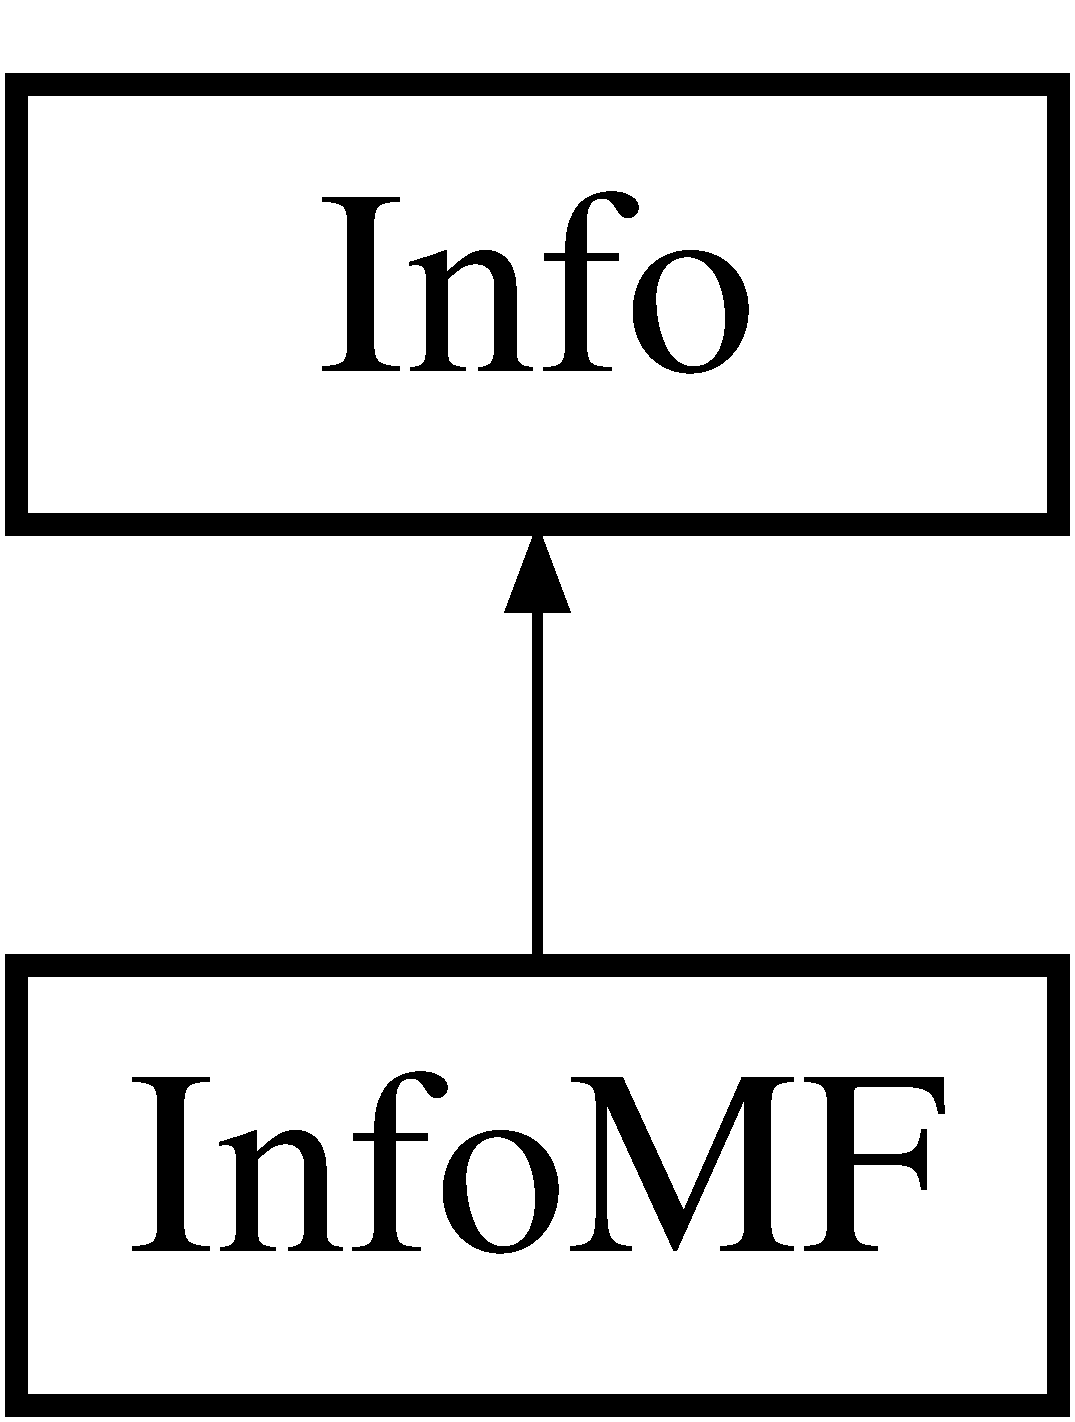
\includegraphics[height=2.000000cm]{class_info_m_f}
\end{center}
\end{figure}
\subsection*{Public Member Functions}
\begin{DoxyCompactItemize}
\item 
\hyperlink{class_info_m_f_ab5ee5aa88e26c288415c6f29545e0279}{Info\+MF} (\hyperlink{class_fraction}{Fraction} \hyperlink{class_info_ae893be5aad319de5d911c3f80cc0a2d4}{training\+Freq}, unsigned int \hyperlink{class_info_aabdfdb282f3ceaae1772574bf2b3cd86}{yellow\+Cards}, unsigned int \hyperlink{class_info_a953c30accc7e6ff301542adfd5824f38}{red\+Cards}, unsigned int \hyperlink{class_info_aecdd57d96490b16a0c2590dd8f34009e}{tackles}, unsigned int \hyperlink{class_info_a2f90c84ba67c0e225dd58cdc14ab7f3d}{fouls}, unsigned int \hyperlink{class_info_a5ad5f72833856502b9c1f6ea50a98619}{goals\+Scored}, unsigned int \hyperlink{class_info_a1c0340af11df3407946b0ffdaae28864}{assists}, \hyperlink{class_fraction}{Fraction} \hyperlink{class_info_a37ee53dc8ae9a9656206e7eb389c6392}{pass\+Accuracy}, vector$<$ \hyperlink{_utils_8hpp_a9f9328fe291d23e820ad594679abd217}{Midfielder\+Position} $>$ \hyperlink{class_info_m_f_ac0ef77d22b8f5c008b8f66034ad0bd81}{positions})
\begin{DoxyCompactList}\small\item\em \hyperlink{class_info_m_f}{Info\+MF}\textquotesingle{}s constructors. \end{DoxyCompactList}\item 
\hyperlink{class_info_m_f_a3b9abc88e1fd6dc2496f3bfec1715735}{Info\+MF} (string \&new\+Info)
\begin{DoxyCompactList}\small\item\em Constructor that creates new midfielder\textquotesingle{}s performance information by reading it from athletes file using a string \end{DoxyCompactList}\item 
\hyperlink{class_info_m_f_af12fdf83050564420b270599b2d8612b}{Info\+MF} ()
\begin{DoxyCompactList}\small\item\em Default constructor. \end{DoxyCompactList}\item 
\hyperlink{class_info_m_f_a30dc23356ceb270ca5ca5f7f2a943245}{Info\+MF} (istream \&in\+Stream)
\begin{DoxyCompactList}\small\item\em Constructor that creates new midfielder\textquotesingle{}s performance information by reading it from thae athletes file using a stringstream. \end{DoxyCompactList}\item 
vector$<$ \hyperlink{_utils_8hpp_a9f9328fe291d23e820ad594679abd217}{Midfielder\+Position} $>$ \hyperlink{class_info_m_f_a1f91cbfd828fdfd6970a3b91b5c04945}{get\+Midfielder\+Specific\+Positions} () const
\begin{DoxyCompactList}\small\item\em Gets the vector containing midfielder specific positions. \end{DoxyCompactList}\item 
void \hyperlink{class_info_m_f_a9b6f1e8cd28291746e3bf51863e1c7b0}{add\+Midfielder\+Specific\+Position} (\hyperlink{_utils_8hpp_a9f9328fe291d23e820ad594679abd217}{Midfielder\+Position} new\+Pos)
\begin{DoxyCompactList}\small\item\em Adds a midfielder specific position to the vector containing the different positions of the midfielder. \end{DoxyCompactList}\item 
string \hyperlink{class_info_m_f_ac61b01c6bfed2c31bd4ddbc2baba097d}{generate\+String} () const
\begin{DoxyCompactList}\small\item\em Generates a string containing the midfielder\textquotesingle{}s performance information. \end{DoxyCompactList}\item 
void \hyperlink{class_info_m_f_a937a1514afaedfa94b2f5372f91edce5}{operator+=} (const \hyperlink{class_info}{Info} $\ast$info2)
\begin{DoxyCompactList}\small\item\em Addition assignment operator that adds two different blocks of midfielder\textquotesingle{}s performance information. \end{DoxyCompactList}\end{DoxyCompactItemize}
\subsection*{Protected Attributes}
\begin{DoxyCompactItemize}
\item 
vector$<$ \hyperlink{_utils_8hpp_a9f9328fe291d23e820ad594679abd217}{Midfielder\+Position} $>$ \hyperlink{class_info_m_f_ac0ef77d22b8f5c008b8f66034ad0bd81}{positions}
\begin{DoxyCompactList}\small\item\em vector containing the different midfielder positions. \end{DoxyCompactList}\end{DoxyCompactItemize}


\subsection{Detailed Description}
A \hyperlink{class_midfielder}{Midfielder}\textquotesingle{}s performance information. 

Luís, 20/11/2016. 

\subsection{Constructor \& Destructor Documentation}
\hypertarget{class_info_m_f_ab5ee5aa88e26c288415c6f29545e0279}{}\label{class_info_m_f_ab5ee5aa88e26c288415c6f29545e0279} 
\index{Info\+MF@{Info\+MF}!Info\+MF@{Info\+MF}}
\index{Info\+MF@{Info\+MF}!Info\+MF@{Info\+MF}}
\subsubsection{\texorpdfstring{Info\+M\+F()}{InfoMF()}\hspace{0.1cm}{\footnotesize\ttfamily [1/4]}}
{\footnotesize\ttfamily Info\+M\+F\+::\+Info\+MF (\begin{DoxyParamCaption}\item[{\hyperlink{class_fraction}{Fraction}}]{training\+Freq,  }\item[{unsigned int}]{yellow\+Cards,  }\item[{unsigned int}]{red\+Cards,  }\item[{unsigned int}]{tackles,  }\item[{unsigned int}]{fouls,  }\item[{unsigned int}]{goals\+Scored,  }\item[{unsigned int}]{assists,  }\item[{\hyperlink{class_fraction}{Fraction}}]{pass\+Accuracy,  }\item[{vector$<$ \hyperlink{_utils_8hpp_a9f9328fe291d23e820ad594679abd217}{Midfielder\+Position} $>$}]{positions }\end{DoxyParamCaption})}



\hyperlink{class_info_m_f}{Info\+MF}\textquotesingle{}s constructors. 

This is a constructor that creates new midfielder\textquotesingle{}s performance information using training frequency, number of yellow cards, number of red cards, number of tackles, number of fouls commited, number of goals scored, number of assists, pass accuracy 

Constructor. 

Luís, 20/11/2016. 


\begin{DoxyParams}{Parameters}
{\em training\+Freq} & The training frequency. \\
\hline
{\em yellow\+Cards} & The yellow cards. \\
\hline
{\em red\+Cards} & The red cards. \\
\hline
{\em tackles} & The tackles. \\
\hline
{\em fouls} & The fouls. \\
\hline
{\em goals\+Scored} & The goals scored. \\
\hline
{\em assists} & The assists. \\
\hline
{\em pass\+Accuracy} & The pass accuracy. \\
\hline
{\em positions} & The positions. \\
\hline
\end{DoxyParams}
\hypertarget{class_info_m_f_a3b9abc88e1fd6dc2496f3bfec1715735}{}\label{class_info_m_f_a3b9abc88e1fd6dc2496f3bfec1715735} 
\index{Info\+MF@{Info\+MF}!Info\+MF@{Info\+MF}}
\index{Info\+MF@{Info\+MF}!Info\+MF@{Info\+MF}}
\subsubsection{\texorpdfstring{Info\+M\+F()}{InfoMF()}\hspace{0.1cm}{\footnotesize\ttfamily [2/4]}}
{\footnotesize\ttfamily Info\+M\+F\+::\+Info\+MF (\begin{DoxyParamCaption}\item[{string \&}]{new\+Info }\end{DoxyParamCaption})}



Constructor that creates new midfielder\textquotesingle{}s performance information by reading it from athletes file using a string 

This is a constructor that creates new midfielder\textquotesingle{}s performance information by reading it from athletes file using a string
\begin{DoxyItemize}
\item / . 
\end{DoxyItemize}

Luís, 20/11/2016. 


\begin{DoxyParams}{Parameters}
{\em new\+Info} & \mbox{[}in,out\mbox{]} Information describing the new. \\
\hline
\end{DoxyParams}
\hypertarget{class_info_m_f_af12fdf83050564420b270599b2d8612b}{}\label{class_info_m_f_af12fdf83050564420b270599b2d8612b} 
\index{Info\+MF@{Info\+MF}!Info\+MF@{Info\+MF}}
\index{Info\+MF@{Info\+MF}!Info\+MF@{Info\+MF}}
\subsubsection{\texorpdfstring{Info\+M\+F()}{InfoMF()}\hspace{0.1cm}{\footnotesize\ttfamily [3/4]}}
{\footnotesize\ttfamily Info\+M\+F\+::\+Info\+MF (\begin{DoxyParamCaption}{ }\end{DoxyParamCaption})}



Default constructor. 

This is the \hyperlink{class_info_m_f}{Info\+MF}\textquotesingle{}s class empty constructor

Luís, 20/11/2016. \hypertarget{class_info_m_f_a30dc23356ceb270ca5ca5f7f2a943245}{}\label{class_info_m_f_a30dc23356ceb270ca5ca5f7f2a943245} 
\index{Info\+MF@{Info\+MF}!Info\+MF@{Info\+MF}}
\index{Info\+MF@{Info\+MF}!Info\+MF@{Info\+MF}}
\subsubsection{\texorpdfstring{Info\+M\+F()}{InfoMF()}\hspace{0.1cm}{\footnotesize\ttfamily [4/4]}}
{\footnotesize\ttfamily Info\+M\+F\+::\+Info\+MF (\begin{DoxyParamCaption}\item[{istream \&}]{in\+Stream }\end{DoxyParamCaption})}



Constructor that creates new midfielder\textquotesingle{}s performance information by reading it from thae athletes file using a stringstream. 

This is a constructor that creates new midfielder\textquotesingle{}s performance information by reading it from thae athletes file using a stringstream

Luís, 20/11/2016. 


\begin{DoxyParams}{Parameters}
{\em in\+Stream} & \mbox{[}in,out\mbox{]} Stream to read data from. \\
\hline
\end{DoxyParams}


\subsection{Member Function Documentation}
\hypertarget{class_info_m_f_a9b6f1e8cd28291746e3bf51863e1c7b0}{}\label{class_info_m_f_a9b6f1e8cd28291746e3bf51863e1c7b0} 
\index{Info\+MF@{Info\+MF}!add\+Midfielder\+Specific\+Position@{add\+Midfielder\+Specific\+Position}}
\index{add\+Midfielder\+Specific\+Position@{add\+Midfielder\+Specific\+Position}!Info\+MF@{Info\+MF}}
\subsubsection{\texorpdfstring{add\+Midfielder\+Specific\+Position()}{addMidfielderSpecificPosition()}}
{\footnotesize\ttfamily void Info\+M\+F\+::add\+Midfielder\+Specific\+Position (\begin{DoxyParamCaption}\item[{\hyperlink{_utils_8hpp_a9f9328fe291d23e820ad594679abd217}{Midfielder\+Position}}]{new\+Pos }\end{DoxyParamCaption})\hspace{0.3cm}{\ttfamily [virtual]}}



Adds a midfielder specific position to the vector containing the different positions of the midfielder. 

This is a method that adds a specific midfielder position to the vector containing the different positions of the midfielder

Luís, 20/11/2016. 


\begin{DoxyParams}{Parameters}
{\em new\+Pos} & The new position. \\
\hline
\end{DoxyParams}


Reimplemented from \hyperlink{class_info_ad90cc81b8a235763cf4127d90aa3a66a}{Info}.

\hypertarget{class_info_m_f_ac61b01c6bfed2c31bd4ddbc2baba097d}{}\label{class_info_m_f_ac61b01c6bfed2c31bd4ddbc2baba097d} 
\index{Info\+MF@{Info\+MF}!generate\+String@{generate\+String}}
\index{generate\+String@{generate\+String}!Info\+MF@{Info\+MF}}
\subsubsection{\texorpdfstring{generate\+String()}{generateString()}}
{\footnotesize\ttfamily string Info\+M\+F\+::generate\+String (\begin{DoxyParamCaption}{ }\end{DoxyParamCaption}) const\hspace{0.3cm}{\ttfamily [virtual]}}



Generates a string containing the midfielder\textquotesingle{}s performance information. 

This is a method that generates a string containing the midfielder\textquotesingle{}s performance information

Luís, 20/11/2016. 

\begin{DoxyReturn}{Returns}
The string. 
\end{DoxyReturn}


Reimplemented from \hyperlink{class_info_a5e52b35a9c17b58222bb57af16c16ce3}{Info}.

\hypertarget{class_info_m_f_a1f91cbfd828fdfd6970a3b91b5c04945}{}\label{class_info_m_f_a1f91cbfd828fdfd6970a3b91b5c04945} 
\index{Info\+MF@{Info\+MF}!get\+Midfielder\+Specific\+Positions@{get\+Midfielder\+Specific\+Positions}}
\index{get\+Midfielder\+Specific\+Positions@{get\+Midfielder\+Specific\+Positions}!Info\+MF@{Info\+MF}}
\subsubsection{\texorpdfstring{get\+Midfielder\+Specific\+Positions()}{getMidfielderSpecificPositions()}}
{\footnotesize\ttfamily vector$<$ \hyperlink{_utils_8hpp_a9f9328fe291d23e820ad594679abd217}{Midfielder\+Position} $>$ Info\+M\+F\+::get\+Midfielder\+Specific\+Positions (\begin{DoxyParamCaption}{ }\end{DoxyParamCaption}) const\hspace{0.3cm}{\ttfamily [virtual]}}



Gets the vector containing midfielder specific positions. 

This is a method that gets the vector containing the different positions of the midfielder

Luís, 20/11/2016. 

\begin{DoxyReturn}{Returns}
The midfielder specific positions. 
\end{DoxyReturn}


Reimplemented from \hyperlink{class_info_afb5cbe001c15498897fc4852bd08c114}{Info}.

\hypertarget{class_info_m_f_a937a1514afaedfa94b2f5372f91edce5}{}\label{class_info_m_f_a937a1514afaedfa94b2f5372f91edce5} 
\index{Info\+MF@{Info\+MF}!operator+=@{operator+=}}
\index{operator+=@{operator+=}!Info\+MF@{Info\+MF}}
\subsubsection{\texorpdfstring{operator+=()}{operator+=()}}
{\footnotesize\ttfamily void Info\+M\+F\+::operator+= (\begin{DoxyParamCaption}\item[{const \hyperlink{class_info}{Info} $\ast$}]{info2 }\end{DoxyParamCaption})\hspace{0.3cm}{\ttfamily [virtual]}}



Addition assignment operator that adds two different blocks of midfielder\textquotesingle{}s performance information. 

This is an assignment operator that adds two different blocks of midfielder\textquotesingle{}s performance information

Luís, 20/11/2016. 


\begin{DoxyParams}{Parameters}
{\em info2} & The second block information. \\
\hline
\end{DoxyParams}


Reimplemented from \hyperlink{class_info_a35d820d35f8ab3b8de15cdfc07f0c5a4}{Info}.



\subsection{Member Data Documentation}
\hypertarget{class_info_m_f_ac0ef77d22b8f5c008b8f66034ad0bd81}{}\label{class_info_m_f_ac0ef77d22b8f5c008b8f66034ad0bd81} 
\index{Info\+MF@{Info\+MF}!positions@{positions}}
\index{positions@{positions}!Info\+MF@{Info\+MF}}
\subsubsection{\texorpdfstring{positions}{positions}}
{\footnotesize\ttfamily vector$<$\hyperlink{_utils_8hpp_a9f9328fe291d23e820ad594679abd217}{Midfielder\+Position}$>$ Info\+M\+F\+::positions\hspace{0.3cm}{\ttfamily [protected]}}



vector containing the different midfielder positions. 



The documentation for this class was generated from the following files\+:\begin{DoxyCompactItemize}
\item 
\hyperlink{_info_athletes_8hpp}{Info\+Athletes.\+hpp}\item 
\hyperlink{_info_athletes_8cpp}{Info\+Athletes.\+cpp}\end{DoxyCompactItemize}

\hypertarget{class_invalid_date}{}\section{Invalid\+Date Class Reference}
\label{class_invalid_date}\index{Invalid\+Date@{Invalid\+Date}}


An invalid date.  




{\ttfamily \#include $<$Exceptions.\+hpp$>$}

\subsection*{Public Member Functions}
\begin{DoxyCompactItemize}
\item 
\hyperlink{class_invalid_date_a8f1350a762e69ee7fab3d96b8ec87455}{Invalid\+Date} (\hyperlink{_exceptions_8hpp_a3c07f150c56e3659483593a47dafc0e3}{Date\+Exception\+Type} \hyperlink{class_invalid_date_a2ec333a89688d1f90713e647720ffda1}{type}, int \hyperlink{class_invalid_date_ae88b81c9928d9f962229b4b60b1ca6e6}{day}, int \hyperlink{class_invalid_date_a63d1eb8cc29192ed24a608efaf8bb841}{month}, int \hyperlink{class_invalid_date_a796e1aee06941892afc67b4ebbbd84c3}{year}, string \hyperlink{class_invalid_date_ae3e99c48b2b32f9f88f1393f1d331ac8}{min\+Date}=\char`\"{}\char`\"{}, string \hyperlink{class_invalid_date_aa7a1be9dd6f1df990c62734800381c2a}{max\+Date}=\char`\"{}\char`\"{})
\begin{DoxyCompactList}\small\item\em Constructor. \end{DoxyCompactList}\item 
string \hyperlink{class_invalid_date_a45284da771728ac2840c252fd261acb5}{get\+Message} ()
\begin{DoxyCompactList}\small\item\em Constructor. \end{DoxyCompactList}\end{DoxyCompactItemize}
\subsection*{Private Attributes}
\begin{DoxyCompactItemize}
\item 
int \hyperlink{class_invalid_date_ae88b81c9928d9f962229b4b60b1ca6e6}{day}
\begin{DoxyCompactList}\small\item\em The day. \end{DoxyCompactList}\item 
int \hyperlink{class_invalid_date_a63d1eb8cc29192ed24a608efaf8bb841}{month}
\begin{DoxyCompactList}\small\item\em The month. \end{DoxyCompactList}\item 
int \hyperlink{class_invalid_date_a796e1aee06941892afc67b4ebbbd84c3}{year}
\begin{DoxyCompactList}\small\item\em The year. \end{DoxyCompactList}\item 
\hyperlink{_exceptions_8hpp_a3c07f150c56e3659483593a47dafc0e3}{Date\+Exception\+Type} \hyperlink{class_invalid_date_a2ec333a89688d1f90713e647720ffda1}{type}
\begin{DoxyCompactList}\small\item\em The exception type. \end{DoxyCompactList}\item 
string \hyperlink{class_invalid_date_aa7a1be9dd6f1df990c62734800381c2a}{max\+Date}
\item 
string \hyperlink{class_invalid_date_ae3e99c48b2b32f9f88f1393f1d331ac8}{min\+Date}
\item 
string \hyperlink{class_invalid_date_add19d43b937e603b19cbf84a993cff91}{exception\+Message}
\begin{DoxyCompactList}\small\item\em Message describing the exception. \end{DoxyCompactList}\end{DoxyCompactItemize}


\subsection{Detailed Description}
An invalid date. 

Luís, 20/11/2016. 

\subsection{Constructor \& Destructor Documentation}
\hypertarget{class_invalid_date_a8f1350a762e69ee7fab3d96b8ec87455}{}\label{class_invalid_date_a8f1350a762e69ee7fab3d96b8ec87455} 
\index{Invalid\+Date@{Invalid\+Date}!Invalid\+Date@{Invalid\+Date}}
\index{Invalid\+Date@{Invalid\+Date}!Invalid\+Date@{Invalid\+Date}}
\subsubsection{\texorpdfstring{Invalid\+Date()}{InvalidDate()}}
{\footnotesize\ttfamily Invalid\+Date\+::\+Invalid\+Date (\begin{DoxyParamCaption}\item[{\hyperlink{_exceptions_8hpp_a3c07f150c56e3659483593a47dafc0e3}{Date\+Exception\+Type}}]{type,  }\item[{int}]{day,  }\item[{int}]{month,  }\item[{int}]{year,  }\item[{string}]{min\+Date = {\ttfamily \char`\"{}\char`\"{}},  }\item[{string}]{max\+Date = {\ttfamily \char`\"{}\char`\"{}} }\end{DoxyParamCaption})}



Constructor. 

Luís, 20/11/2016. 


\begin{DoxyParams}{Parameters}
{\em type} & The date exception type. \\
\hline
{\em day} & The day. \\
\hline
{\em month} & The month. \\
\hline
{\em year} & The year. \\
\hline
\end{DoxyParams}


\subsection{Member Function Documentation}
\hypertarget{class_invalid_date_a45284da771728ac2840c252fd261acb5}{}\label{class_invalid_date_a45284da771728ac2840c252fd261acb5} 
\index{Invalid\+Date@{Invalid\+Date}!get\+Message@{get\+Message}}
\index{get\+Message@{get\+Message}!Invalid\+Date@{Invalid\+Date}}
\subsubsection{\texorpdfstring{get\+Message()}{getMessage()}}
{\footnotesize\ttfamily string Invalid\+Date\+::get\+Message (\begin{DoxyParamCaption}{ }\end{DoxyParamCaption})}



Constructor. 

Luís, 20/11/2016. 


\begin{DoxyParams}{Parameters}
{\em exception\+Message} & Message describing the exception. \\
\hline
{\em day} & The day. \\
\hline
{\em month} & The month. \\
\hline
{\em year} & The year. \\
\hline
\end{DoxyParams}


Gets the exception message. 

Luís, 20/11/2016. 

\begin{DoxyReturn}{Returns}
The exception message. 
\end{DoxyReturn}


\subsection{Member Data Documentation}
\hypertarget{class_invalid_date_ae88b81c9928d9f962229b4b60b1ca6e6}{}\label{class_invalid_date_ae88b81c9928d9f962229b4b60b1ca6e6} 
\index{Invalid\+Date@{Invalid\+Date}!day@{day}}
\index{day@{day}!Invalid\+Date@{Invalid\+Date}}
\subsubsection{\texorpdfstring{day}{day}}
{\footnotesize\ttfamily int Invalid\+Date\+::day\hspace{0.3cm}{\ttfamily [private]}}



The day. 

\hypertarget{class_invalid_date_add19d43b937e603b19cbf84a993cff91}{}\label{class_invalid_date_add19d43b937e603b19cbf84a993cff91} 
\index{Invalid\+Date@{Invalid\+Date}!exception\+Message@{exception\+Message}}
\index{exception\+Message@{exception\+Message}!Invalid\+Date@{Invalid\+Date}}
\subsubsection{\texorpdfstring{exception\+Message}{exceptionMessage}}
{\footnotesize\ttfamily string Invalid\+Date\+::exception\+Message\hspace{0.3cm}{\ttfamily [private]}}



Message describing the exception. 

\hypertarget{class_invalid_date_aa7a1be9dd6f1df990c62734800381c2a}{}\label{class_invalid_date_aa7a1be9dd6f1df990c62734800381c2a} 
\index{Invalid\+Date@{Invalid\+Date}!max\+Date@{max\+Date}}
\index{max\+Date@{max\+Date}!Invalid\+Date@{Invalid\+Date}}
\subsubsection{\texorpdfstring{max\+Date}{maxDate}}
{\footnotesize\ttfamily string Invalid\+Date\+::max\+Date\hspace{0.3cm}{\ttfamily [private]}}

\hypertarget{class_invalid_date_ae3e99c48b2b32f9f88f1393f1d331ac8}{}\label{class_invalid_date_ae3e99c48b2b32f9f88f1393f1d331ac8} 
\index{Invalid\+Date@{Invalid\+Date}!min\+Date@{min\+Date}}
\index{min\+Date@{min\+Date}!Invalid\+Date@{Invalid\+Date}}
\subsubsection{\texorpdfstring{min\+Date}{minDate}}
{\footnotesize\ttfamily string Invalid\+Date\+::min\+Date\hspace{0.3cm}{\ttfamily [private]}}

\hypertarget{class_invalid_date_a63d1eb8cc29192ed24a608efaf8bb841}{}\label{class_invalid_date_a63d1eb8cc29192ed24a608efaf8bb841} 
\index{Invalid\+Date@{Invalid\+Date}!month@{month}}
\index{month@{month}!Invalid\+Date@{Invalid\+Date}}
\subsubsection{\texorpdfstring{month}{month}}
{\footnotesize\ttfamily int Invalid\+Date\+::month\hspace{0.3cm}{\ttfamily [private]}}



The month. 

\hypertarget{class_invalid_date_a2ec333a89688d1f90713e647720ffda1}{}\label{class_invalid_date_a2ec333a89688d1f90713e647720ffda1} 
\index{Invalid\+Date@{Invalid\+Date}!type@{type}}
\index{type@{type}!Invalid\+Date@{Invalid\+Date}}
\subsubsection{\texorpdfstring{type}{type}}
{\footnotesize\ttfamily \hyperlink{_exceptions_8hpp_a3c07f150c56e3659483593a47dafc0e3}{Date\+Exception\+Type} Invalid\+Date\+::type\hspace{0.3cm}{\ttfamily [private]}}



The exception type. 

\hypertarget{class_invalid_date_a796e1aee06941892afc67b4ebbbd84c3}{}\label{class_invalid_date_a796e1aee06941892afc67b4ebbbd84c3} 
\index{Invalid\+Date@{Invalid\+Date}!year@{year}}
\index{year@{year}!Invalid\+Date@{Invalid\+Date}}
\subsubsection{\texorpdfstring{year}{year}}
{\footnotesize\ttfamily int Invalid\+Date\+::year\hspace{0.3cm}{\ttfamily [private]}}



The year. 



The documentation for this class was generated from the following files\+:\begin{DoxyCompactItemize}
\item 
\hyperlink{_exceptions_8hpp}{Exceptions.\+hpp}\item 
\hyperlink{_exceptions_8cpp}{Exceptions.\+cpp}\end{DoxyCompactItemize}

\hypertarget{class_invalid_input}{}\section{Invalid\+Input Class Reference}
\label{class_invalid_input}\index{Invalid\+Input@{Invalid\+Input}}


An invalid input.  




{\ttfamily \#include $<$Exceptions.\+hpp$>$}

\subsection*{Public Member Functions}
\begin{DoxyCompactItemize}
\item 
\hyperlink{class_invalid_input_a0b7eb468e727adcd94e87e5a8c0cf716}{Invalid\+Input} (string \hyperlink{class_invalid_input_a0b76d2656afecfe458b1cc1a87dd98c9}{exception\+Message}=\char`\"{}Invalid Input\char`\"{})
\begin{DoxyCompactList}\small\item\em Constructor. \end{DoxyCompactList}\item 
string \hyperlink{class_invalid_input_abe61234c3ad05ac96a76f6adbba4b377}{get\+Message} ()
\begin{DoxyCompactList}\small\item\em Gets the exception message. \end{DoxyCompactList}\end{DoxyCompactItemize}
\subsection*{Private Attributes}
\begin{DoxyCompactItemize}
\item 
string \hyperlink{class_invalid_input_a0b76d2656afecfe458b1cc1a87dd98c9}{exception\+Message}
\begin{DoxyCompactList}\small\item\em Message describing the exception. \end{DoxyCompactList}\end{DoxyCompactItemize}


\subsection{Detailed Description}
An invalid input. 

Luís, 20/11/2016. 

\subsection{Constructor \& Destructor Documentation}
\hypertarget{class_invalid_input_a0b7eb468e727adcd94e87e5a8c0cf716}{}\label{class_invalid_input_a0b7eb468e727adcd94e87e5a8c0cf716} 
\index{Invalid\+Input@{Invalid\+Input}!Invalid\+Input@{Invalid\+Input}}
\index{Invalid\+Input@{Invalid\+Input}!Invalid\+Input@{Invalid\+Input}}
\subsubsection{\texorpdfstring{Invalid\+Input()}{InvalidInput()}}
{\footnotesize\ttfamily Invalid\+Input\+::\+Invalid\+Input (\begin{DoxyParamCaption}\item[{string}]{exception\+Message = {\ttfamily \char`\"{}Invalid~Input\char`\"{}} }\end{DoxyParamCaption})}



Constructor. 

Luís, 20/11/2016. 


\begin{DoxyParams}{Parameters}
{\em exception\+Message} & Message describing the exception. \\
\hline
\end{DoxyParams}


\subsection{Member Function Documentation}
\hypertarget{class_invalid_input_abe61234c3ad05ac96a76f6adbba4b377}{}\label{class_invalid_input_abe61234c3ad05ac96a76f6adbba4b377} 
\index{Invalid\+Input@{Invalid\+Input}!get\+Message@{get\+Message}}
\index{get\+Message@{get\+Message}!Invalid\+Input@{Invalid\+Input}}
\subsubsection{\texorpdfstring{get\+Message()}{getMessage()}}
{\footnotesize\ttfamily string Invalid\+Input\+::get\+Message (\begin{DoxyParamCaption}{ }\end{DoxyParamCaption})}



Gets the exception message. 

Luís, 20/11/2016. 

\begin{DoxyReturn}{Returns}
The exception message. 
\end{DoxyReturn}


\subsection{Member Data Documentation}
\hypertarget{class_invalid_input_a0b76d2656afecfe458b1cc1a87dd98c9}{}\label{class_invalid_input_a0b76d2656afecfe458b1cc1a87dd98c9} 
\index{Invalid\+Input@{Invalid\+Input}!exception\+Message@{exception\+Message}}
\index{exception\+Message@{exception\+Message}!Invalid\+Input@{Invalid\+Input}}
\subsubsection{\texorpdfstring{exception\+Message}{exceptionMessage}}
{\footnotesize\ttfamily string Invalid\+Input\+::exception\+Message\hspace{0.3cm}{\ttfamily [private]}}



Message describing the exception. 



The documentation for this class was generated from the following files\+:\begin{DoxyCompactItemize}
\item 
\hyperlink{_exceptions_8hpp}{Exceptions.\+hpp}\item 
\hyperlink{_exceptions_8cpp}{Exceptions.\+cpp}\end{DoxyCompactItemize}

\hypertarget{class_invalid_stream}{}\section{Invalid\+Stream Class Reference}
\label{class_invalid_stream}\index{Invalid\+Stream@{Invalid\+Stream}}


An invalid stream.  




{\ttfamily \#include $<$Exceptions.\+hpp$>$}

\subsection*{Public Member Functions}
\begin{DoxyCompactItemize}
\item 
\hyperlink{class_invalid_stream_ab1b3ef87fa02f66bd2709efd48ad3928}{Invalid\+Stream} (string \hyperlink{class_invalid_stream_abec03af0cdc07c0e52aa7a1daadd438c}{file\+Name}, \hyperlink{_exceptions_8hpp_a20debbce0a9d256d07eac93067032a39}{Invalid\+Stream\+Type} \hyperlink{class_invalid_stream_af18ab97f0a3db6cc76716b1bd7808832}{type})
\begin{DoxyCompactList}\small\item\em Constructor. \end{DoxyCompactList}\item 
string \hyperlink{class_invalid_stream_a8aa15b0bc9caa1a31b15cfcbebaad67b}{get\+Message} ()
\begin{DoxyCompactList}\small\item\em Gets the exception message. \end{DoxyCompactList}\end{DoxyCompactItemize}
\subsection*{Private Attributes}
\begin{DoxyCompactItemize}
\item 
string \hyperlink{class_invalid_stream_abec03af0cdc07c0e52aa7a1daadd438c}{file\+Name}
\begin{DoxyCompactList}\small\item\em Filename of the file. \end{DoxyCompactList}\item 
\hyperlink{_exceptions_8hpp_a20debbce0a9d256d07eac93067032a39}{Invalid\+Stream\+Type} \hyperlink{class_invalid_stream_af18ab97f0a3db6cc76716b1bd7808832}{type}
\begin{DoxyCompactList}\small\item\em The type. \end{DoxyCompactList}\end{DoxyCompactItemize}


\subsection{Detailed Description}
An invalid stream. 

Luís, 20/11/2016. 

\subsection{Constructor \& Destructor Documentation}
\hypertarget{class_invalid_stream_ab1b3ef87fa02f66bd2709efd48ad3928}{}\label{class_invalid_stream_ab1b3ef87fa02f66bd2709efd48ad3928} 
\index{Invalid\+Stream@{Invalid\+Stream}!Invalid\+Stream@{Invalid\+Stream}}
\index{Invalid\+Stream@{Invalid\+Stream}!Invalid\+Stream@{Invalid\+Stream}}
\subsubsection{\texorpdfstring{Invalid\+Stream()}{InvalidStream()}}
{\footnotesize\ttfamily Invalid\+Stream\+::\+Invalid\+Stream (\begin{DoxyParamCaption}\item[{string}]{file\+Name,  }\item[{\hyperlink{_exceptions_8hpp_a20debbce0a9d256d07eac93067032a39}{Invalid\+Stream\+Type}}]{type }\end{DoxyParamCaption})}



Constructor. 

Luís, 20/11/2016. 


\begin{DoxyParams}{Parameters}
{\em file\+Name} & Filename of the file. \\
\hline
{\em type} & The exception type. \\
\hline
\end{DoxyParams}


\subsection{Member Function Documentation}
\hypertarget{class_invalid_stream_a8aa15b0bc9caa1a31b15cfcbebaad67b}{}\label{class_invalid_stream_a8aa15b0bc9caa1a31b15cfcbebaad67b} 
\index{Invalid\+Stream@{Invalid\+Stream}!get\+Message@{get\+Message}}
\index{get\+Message@{get\+Message}!Invalid\+Stream@{Invalid\+Stream}}
\subsubsection{\texorpdfstring{get\+Message()}{getMessage()}}
{\footnotesize\ttfamily string Invalid\+Stream\+::get\+Message (\begin{DoxyParamCaption}{ }\end{DoxyParamCaption})}



Gets the exception message. 

Luís, 20/11/2016. 

\begin{DoxyReturn}{Returns}
The exception message. 
\end{DoxyReturn}


\subsection{Member Data Documentation}
\hypertarget{class_invalid_stream_abec03af0cdc07c0e52aa7a1daadd438c}{}\label{class_invalid_stream_abec03af0cdc07c0e52aa7a1daadd438c} 
\index{Invalid\+Stream@{Invalid\+Stream}!file\+Name@{file\+Name}}
\index{file\+Name@{file\+Name}!Invalid\+Stream@{Invalid\+Stream}}
\subsubsection{\texorpdfstring{file\+Name}{fileName}}
{\footnotesize\ttfamily string Invalid\+Stream\+::file\+Name\hspace{0.3cm}{\ttfamily [private]}}



Filename of the file. 

\hypertarget{class_invalid_stream_af18ab97f0a3db6cc76716b1bd7808832}{}\label{class_invalid_stream_af18ab97f0a3db6cc76716b1bd7808832} 
\index{Invalid\+Stream@{Invalid\+Stream}!type@{type}}
\index{type@{type}!Invalid\+Stream@{Invalid\+Stream}}
\subsubsection{\texorpdfstring{type}{type}}
{\footnotesize\ttfamily \hyperlink{_exceptions_8hpp_a20debbce0a9d256d07eac93067032a39}{Invalid\+Stream\+Type} Invalid\+Stream\+::type\hspace{0.3cm}{\ttfamily [private]}}



The type. 



The documentation for this class was generated from the following files\+:\begin{DoxyCompactItemize}
\item 
\hyperlink{_exceptions_8hpp}{Exceptions.\+hpp}\item 
\hyperlink{_exceptions_8cpp}{Exceptions.\+cpp}\end{DoxyCompactItemize}

\hypertarget{class_level}{}\section{Level Class Reference}
\label{class_level}\index{Level@{Level}}


{\ttfamily \#include $<$Level.\+h$>$}

\subsection*{Public Member Functions}
\begin{DoxyCompactItemize}
\item 
\hyperlink{class_level_a3e56499129f883f0cb4e5a855243c1e2}{Level} (string \hyperlink{class_level_a39e8e8b8d5f64c3d3a50b617c3ea8321}{year\+Of\+Season}, string path\+To\+Season\+Folder, string \hyperlink{class_level_aa59964368a47b0d36ff67948b880b3ef}{level\+Name}, \hyperlink{class_club}{Club} $\ast$\hyperlink{class_level_a383670d611a12c518ef48ce9fa179f7a}{parent\+Club})
\begin{DoxyCompactList}\small\item\em Constructor. \end{DoxyCompactList}\item 
unsigned int \hyperlink{class_level_ab773a1c1c9ecfa31c45d5e3e48b38a92}{get\+Min\+Age} () const
\begin{DoxyCompactList}\small\item\em Gets minimum age. \end{DoxyCompactList}\item 
unsigned int \hyperlink{class_level_ae034a3eb28a90653820eb9633b9f7464}{get\+Max\+Age} () const
\begin{DoxyCompactList}\small\item\em Gets maximum age. \end{DoxyCompactList}\item 
char \hyperlink{class_level_a1a32dbbb6c0a3e9cfd26870388a02363}{get\+Min\+Height} () const
\begin{DoxyCompactList}\small\item\em Gets minimum height. \end{DoxyCompactList}\item 
map$<$ unsigned int, \hyperlink{class_info}{Info} $\ast$ $>$ \hyperlink{class_level_a3d4498069e112cbdc952ce1c9e5eb6a5}{get\+Map\+Info\+Players} () const
\begin{DoxyCompactList}\small\item\em Gets the map containing the athletes performance informations. \end{DoxyCompactList}\item 
vector$<$ unsigned int $>$ \hyperlink{class_level_a2130d8ee6b56f18821e5606c757661d3}{get\+Coaches} () const
\begin{DoxyCompactList}\small\item\em Gets the coaches. \end{DoxyCompactList}\item 
\hyperlink{class_level}{Level} $\ast$ \hyperlink{class_level_a5c9636031654943ea260c22fe5dede44}{add\+Athlete\+To\+Level} (pair$<$ unsigned int, \hyperlink{class_info}{Info} $\ast$$>$ player\+Info)
\begin{DoxyCompactList}\small\item\em Adds an athlete to level. \end{DoxyCompactList}\item 
\hyperlink{class_level}{Level} $\ast$ \hyperlink{class_level_ae0c356fc3ffa08c834d4a9ea3d7bacc8}{add\+Coach\+To\+Level} (unsigned int id\+Coach, bool main\+Coach=false)
\begin{DoxyCompactList}\small\item\em Adds a coach to level to \textquotesingle{}main\+Coach\textquotesingle{}. \end{DoxyCompactList}\item 
vector$<$ \hyperlink{class_tournament}{Tournament} $\ast$ $>$ \hyperlink{class_level_ad01baca6bdb906c6d605f04f6885cb81}{get\+Tournaments} () const
\begin{DoxyCompactList}\small\item\em Gets the tournaments. \end{DoxyCompactList}\item 
string \hyperlink{class_level_a810328bff045bfb02159d388414718d8}{get\+Level\+Name} () const
\begin{DoxyCompactList}\small\item\em Gets level name. \end{DoxyCompactList}\item 
int \hyperlink{class_level_afda6ab0cbba0cea709e2fb04cdc0187a}{get\+Main\+Coach\+Id} () const
\begin{DoxyCompactList}\small\item\em Gets main coach identifier. \end{DoxyCompactList}\item 
string \hyperlink{class_level_a22837fd78482f7a7451cb228fe6595d2}{get\+Year} () const
\begin{DoxyCompactList}\small\item\em Gets the year. \end{DoxyCompactList}\item 
string \hyperlink{class_level_a66ee534fb23e363ccba422c64f08a202}{get\+Path\+To\+Level\+Folder} () const
\begin{DoxyCompactList}\small\item\em Gets path to level folder. \end{DoxyCompactList}\item 
string \hyperlink{class_level_a038f1525cd82ba7ff262c95559ae05f9}{get\+Path\+To\+Level\+Athletes\+File} () const
\begin{DoxyCompactList}\small\item\em Gets path to level athletes file. \end{DoxyCompactList}\item 
string \hyperlink{class_level_ac779bf1052984fbcba0669139e639c46}{get\+Path\+To\+Level\+Coaches\+File} () const
\begin{DoxyCompactList}\small\item\em Gets path to level coaches file. \end{DoxyCompactList}\item 
string \hyperlink{class_level_ac4cd1f4a5c87dbd2b47c1d07cbf114e4}{get\+Path\+To\+Level\+Matches\+File} () const
\begin{DoxyCompactList}\small\item\em Gets path to level matches file. \end{DoxyCompactList}\item 
string \hyperlink{class_level_a5808d2312d1b6c2f93dbbd0b47c97499}{get\+Path\+To\+Level\+Matches\+Folder} () const
\begin{DoxyCompactList}\small\item\em Gets path to level matches folder. \end{DoxyCompactList}\item 
unsigned int \hyperlink{class_level_abe3f06938f9d39800648c0fc0ddbadeb}{get\+Last\+Match\+Id} () const
\begin{DoxyCompactList}\small\item\em Gets the last match identifier. \end{DoxyCompactList}\item 
void \hyperlink{class_level_ad3f226396e776c339ae2a33e4cebd2c3}{update\+Last\+Match\+Id} ()
\begin{DoxyCompactList}\small\item\em Updates the last match identifier. \end{DoxyCompactList}\item 
vector$<$ \hyperlink{class_match}{Match} $\ast$ $>$ \hyperlink{class_level_a67ede4d99accffb562e15c2c75cb81b8}{get\+All\+Level\+Matches} (bool only\+Not\+Played=false) const
\begin{DoxyCompactList}\small\item\em Gets all level matches. \end{DoxyCompactList}\item 
vector$<$ \hyperlink{class_match}{Match} $\ast$ $>$ \hyperlink{class_level_af1da9db30e4e0d350fb72ca7c844958c}{get\+Matches\+Ready\+To\+Play} () const
\begin{DoxyCompactList}\small\item\em Gets matches ready to play. \end{DoxyCompactList}\item 
vector$<$ \hyperlink{class_training}{Training} $\ast$ $>$ \hyperlink{class_level_a839826078b5b56b27b697e7e599dd6ef}{get\+Trainings\+Ready\+To\+Play} () const
\begin{DoxyCompactList}\small\item\em Gets trainings ready be made. \end{DoxyCompactList}\item 
\hyperlink{class_table}{Table} \hyperlink{class_level_aeacdd2b25ba6fdfadb89290dc3d73513}{show\+Athletes\+Of\+Level} (bool only\+Available=false) const
\begin{DoxyCompactList}\small\item\em Shows the athletes of level. \end{DoxyCompactList}\item 
vector$<$ \hyperlink{class_training}{Training} $\ast$ $>$ \hyperlink{class_level_aaf1c5f18fbbc46890d5849ab5bf4eb91}{get\+All\+Level\+Trainings} (bool only\+Not\+Played=false) const
\begin{DoxyCompactList}\small\item\em Gets all level trainings. \end{DoxyCompactList}\item 
\hyperlink{class_level}{Level} $\ast$ \hyperlink{class_level_a7d49f90eae1baaaf957a68334c54ab34}{add\+Match\+To\+Level} (\hyperlink{class_match}{Match} $\ast$new\+Match)
\begin{DoxyCompactList}\small\item\em Adds a match to level. \end{DoxyCompactList}\item 
\hyperlink{class_level}{Level} $\ast$ \hyperlink{class_level_a6bdd904d0268409efd619c49950b9ccc}{add\+Training\+To\+Level} (\hyperlink{class_training}{Training} $\ast$new\+Training)
\begin{DoxyCompactList}\small\item\em Adds a training to level. \end{DoxyCompactList}\item 
void \hyperlink{class_level_ab28a5bc03ae76bb52b44711c4d59e56f}{show\+Matches} (vector$<$ \hyperlink{class_match}{Match} $\ast$$>$ matches)
\begin{DoxyCompactList}\small\item\em Shows the matches. \end{DoxyCompactList}\item 
void \hyperlink{class_level_abe23e553dbe354819966db88317a095c}{show\+Match} (\hyperlink{class_match}{Match} $\ast$match\+To\+Show)
\begin{DoxyCompactList}\small\item\em Shows the match. \end{DoxyCompactList}\item 
void \hyperlink{class_level_a213282facf5cf571e5266013124d0002}{show\+Trainings} (vector$<$ \hyperlink{class_training}{Training} $\ast$$>$ matches)
\begin{DoxyCompactList}\small\item\em Shows the trainings. \end{DoxyCompactList}\item 
void \hyperlink{class_level_a26d032066034ca77792322903d0edfd5}{sort\+Trainings} ()
\begin{DoxyCompactList}\small\item\em Sort trainings. \end{DoxyCompactList}\item 
void \hyperlink{class_level_ab1d7ebab6cd1338ba044dc54fe6fd38b}{save\+Level\+Trainings} () const
\begin{DoxyCompactList}\small\item\em Saves the level trainings. \end{DoxyCompactList}\item 
void \hyperlink{class_level_ac4dc4739fe40da18e9cf19b2a42c7b43}{save\+Level\+Tournaments} () const
\begin{DoxyCompactList}\small\item\em Saves the level tournaments. \end{DoxyCompactList}\item 
void \hyperlink{class_level_aee00ac018e11b0c0fa8a42ee45ac2ae8}{schedule\+Training} (\hyperlink{class_date}{Date} training\+Date)
\begin{DoxyCompactList}\small\item\em Schedule training. \end{DoxyCompactList}\item 
void \hyperlink{class_level_a347646f5e92f549ac4467afb8fc723f1}{register\+Training} (unsigned int training\+Id, vector$<$ unsigned int $>$ missing\+Players)
\begin{DoxyCompactList}\small\item\em Registers scheduled training. \end{DoxyCompactList}\item 
void \hyperlink{class_level_afed5cd2f4b28935b95c6541d6e15c8a0}{register\+Training} (\hyperlink{class_date}{Date} training\+Date, vector$<$ unsigned int $>$ missing\+Players)
\begin{DoxyCompactList}\small\item\em Registers non scheduled training. \end{DoxyCompactList}\item 
\hyperlink{class_table}{Table} \hyperlink{class_level_a49d9f8bc2848dc41199342b1a0557631}{get\+Trainings\+List} (\hyperlink{_training_8hpp_aa44c715f606358e721f7911b15a1cfc5}{Sort\+Criteria} criteria=\hyperlink{_training_8hpp_aa44c715f606358e721f7911b15a1cfc5aa325b226dd9bbe4b1d3989a96326bb43}{date}, \hyperlink{_training_8hpp_ad9be72f666a31b4318bbc8e8a16a9472}{Sort\+Order} order=\hyperlink{_training_8hpp_ad9be72f666a31b4318bbc8e8a16a9472a9c04aeb1f974b5141257e307bcd1610d}{ascending}, char list\+Type=\textquotesingle{}a\textquotesingle{}) const
\begin{DoxyCompactList}\small\item\em Get the all the trainings of the level. \end{DoxyCompactList}\item 
void \hyperlink{class_level_a040a2ff70cc01830e8bd5589deeaf9c8}{add\+Tournament} (\hyperlink{class_date}{Date} initial\+Date, \hyperlink{class_date}{Date} end\+Date, vector$<$ string $>$ tournament\+Clubs, string name)
\begin{DoxyCompactList}\small\item\em Adds a tournament. \end{DoxyCompactList}\item 
vector$<$ vector$<$ string $>$ $>$ \hyperlink{class_level_a71eeac219eb35734461d2fec5ea69f65}{get\+Tournament\+Matches} (unsigned int tournament\+Id) const
\begin{DoxyCompactList}\small\item\em Gets tournament matches. \end{DoxyCompactList}\item 
vector$<$ unsigned int $>$ \hyperlink{class_level_ac5d3ad313fb2694842f245fdb9499872}{filter\+Players} (vector$<$ unsigned int $>$ original\+Player\+Ids\+Vector) const
\begin{DoxyCompactList}\small\item\em Filter players. \end{DoxyCompactList}\item 
\hyperlink{class_club}{Club} $\ast$ \hyperlink{class_level_afa22f5ec13dde3359a636df38cf71377}{get\+Parent\+Club} () const
\begin{DoxyCompactList}\small\item\em Gets the parent club. \end{DoxyCompactList}\end{DoxyCompactItemize}
\subsection*{Private Attributes}
\begin{DoxyCompactItemize}
\item 
\hyperlink{class_club}{Club} $\ast$ \hyperlink{class_level_a383670d611a12c518ef48ce9fa179f7a}{parent\+Club}
\begin{DoxyCompactList}\small\item\em The parent club. \end{DoxyCompactList}\item 
\hyperlink{_utils_8hpp_a226b190c54f09ab6ba8ac83b28e3c4b6}{age\+Level} \hyperlink{class_level_a722b6532d70a38fa5f31518761c63012}{level\+Enum}
\begin{DoxyCompactList}\small\item\em The level enum. \end{DoxyCompactList}\item 
string \hyperlink{class_level_aa59964368a47b0d36ff67948b880b3ef}{level\+Name}
\begin{DoxyCompactList}\small\item\em Name of the level. \end{DoxyCompactList}\item 
string \hyperlink{class_level_a2cb769dac86d869787a3a6cd90f32454}{path\+To\+Level\+Folder}
\begin{DoxyCompactList}\small\item\em Pathname of the path to level folder. \end{DoxyCompactList}\item 
string \hyperlink{class_level_a657f004e4174828d48b1a7014536fa50}{path\+To\+Level\+Athletes\+File}
\begin{DoxyCompactList}\small\item\em The path to level athletes file. \end{DoxyCompactList}\item 
string \hyperlink{class_level_a2c43373a0343a66b777d7e879544b5ae}{path\+To\+Level\+Coaches\+File}
\begin{DoxyCompactList}\small\item\em The path to level coaches file. \end{DoxyCompactList}\item 
string \hyperlink{class_level_a295d863ec897640e286b1f9848a36c46}{path\+To\+Level\+Matches\+File}
\begin{DoxyCompactList}\small\item\em The path to level matches file. \end{DoxyCompactList}\item 
string \hyperlink{class_level_aa13c0c2c38b5cb67f5aa51654710d9a7}{path\+To\+Level\+Matches\+Folder}
\begin{DoxyCompactList}\small\item\em Pathname of the path to level matches folder. \end{DoxyCompactList}\item 
string \hyperlink{class_level_a3958021df480857263d65f57c668f5bd}{path\+To\+Level\+Trainings\+File}
\begin{DoxyCompactList}\small\item\em The path to level trainings file. \end{DoxyCompactList}\item 
string \hyperlink{class_level_a1c196300430057e2d7d133e85f0c929a}{path\+To\+Level\+Tournaments\+File}
\begin{DoxyCompactList}\small\item\em The path to level tournaments file. \end{DoxyCompactList}\item 
string \hyperlink{class_level_a49f20ede8543a270f763f7253c4247d6}{path\+To\+Level\+Tournaments\+Folder}
\begin{DoxyCompactList}\small\item\em Pathname of the path to level tournaments folder. \end{DoxyCompactList}\item 
string \hyperlink{class_level_a39e8e8b8d5f64c3d3a50b617c3ea8321}{year\+Of\+Season}
\begin{DoxyCompactList}\small\item\em The year of season. \end{DoxyCompactList}\item 
unsigned int \hyperlink{class_level_a4c6c8eb32ad6dbc8b7dae820de6db4ba}{last\+Match\+Id}
\begin{DoxyCompactList}\small\item\em Identifier for the last match. \end{DoxyCompactList}\item 
vector$<$ \hyperlink{class_match}{Match} $\ast$ $>$ \hyperlink{class_level_ace54062d1ad170581337f33ac4d6ab45}{level\+Matches}
\begin{DoxyCompactList}\small\item\em The level matches. \end{DoxyCompactList}\item 
vector$<$ \hyperlink{class_training}{Training} $\ast$ $>$ \hyperlink{class_level_a887624d3374e9ba74edfeb6a5a38a4b1}{level\+Trainings}
\begin{DoxyCompactList}\small\item\em The level trainings. \end{DoxyCompactList}\item 
int \hyperlink{class_level_af7943487f1cf311dfa00400037da1f3d}{level\+Main\+Coach}
\begin{DoxyCompactList}\small\item\em The level main coach. \end{DoxyCompactList}\item 
vector$<$ unsigned int $>$ \hyperlink{class_level_a2244ded7cbc3e261c400042dcd1f765f}{coaches\+Ids\+Vector}
\begin{DoxyCompactList}\small\item\em The coaches identifiers vector. \end{DoxyCompactList}\item 
map$<$ unsigned int, \hyperlink{class_info}{Info} $\ast$ $>$ \hyperlink{class_level_aea430b89c484e79aebe7f23852ce998c}{map\+Info\+Players}
\begin{DoxyCompactList}\small\item\em The map information players. \end{DoxyCompactList}\item 
unsigned int \hyperlink{class_level_a3ab82616194caca77f24c568c4151a19}{min\+Age}
\begin{DoxyCompactList}\small\item\em The minimum age. \end{DoxyCompactList}\item 
unsigned int \hyperlink{class_level_a009aecf3fb4c0b553680d9e66385a8e2}{max\+Age}
\begin{DoxyCompactList}\small\item\em The maximum age. \end{DoxyCompactList}\item 
char \hyperlink{class_level_a94edfb0b68503e60c1d79163c2cc1861}{min\+Height}
\begin{DoxyCompactList}\small\item\em The minimum height. \end{DoxyCompactList}\item 
vector$<$ \hyperlink{class_tournament}{Tournament} $\ast$ $>$ \hyperlink{class_level_ad6c327fa0c1fc11c38bc167de8e92476}{tournaments}
\begin{DoxyCompactList}\small\item\em The tournaments. \end{DoxyCompactList}\end{DoxyCompactItemize}


\subsection{Constructor \& Destructor Documentation}
\hypertarget{class_level_a3e56499129f883f0cb4e5a855243c1e2}{}\label{class_level_a3e56499129f883f0cb4e5a855243c1e2} 
\index{Level@{Level}!Level@{Level}}
\index{Level@{Level}!Level@{Level}}
\subsubsection{\texorpdfstring{Level()}{Level()}}
{\footnotesize\ttfamily Level\+::\+Level (\begin{DoxyParamCaption}\item[{string}]{year\+Of\+Season,  }\item[{string}]{path\+To\+Season\+Folder,  }\item[{string}]{level\+Name,  }\item[{\hyperlink{class_club}{Club} $\ast$}]{parent\+Club }\end{DoxyParamCaption})}



Constructor. 

Luís, 20/11/2016. 


\begin{DoxyParams}{Parameters}
{\em year\+Of\+Season} & The year of season. \\
\hline
{\em path\+To\+Season\+Folder} & Pathname of the path to season folder. \\
\hline
{\em level\+Name} & Name of the level. \\
\hline
{\em parent\+Club} & \mbox{[}in,out\mbox{]} If non-\/null, the parent club. \\
\hline
\end{DoxyParams}


\subsection{Member Function Documentation}
\hypertarget{class_level_a5c9636031654943ea260c22fe5dede44}{}\label{class_level_a5c9636031654943ea260c22fe5dede44} 
\index{Level@{Level}!add\+Athlete\+To\+Level@{add\+Athlete\+To\+Level}}
\index{add\+Athlete\+To\+Level@{add\+Athlete\+To\+Level}!Level@{Level}}
\subsubsection{\texorpdfstring{add\+Athlete\+To\+Level()}{addAthleteToLevel()}}
{\footnotesize\ttfamily \hyperlink{class_level}{Level} $\ast$ Level\+::add\+Athlete\+To\+Level (\begin{DoxyParamCaption}\item[{pair$<$ unsigned int, \hyperlink{class_info}{Info} $\ast$$>$}]{player\+Info }\end{DoxyParamCaption})}



Adds an athlete to level. 

Luís, 20/11/2016. 


\begin{DoxyParams}{Parameters}
{\em player\+Info} & \mbox{[}in,out\mbox{]} If non-\/null, information describing the player. \\
\hline
\end{DoxyParams}


\begin{DoxyReturn}{Returns}
Null if it fails, else a pointer to a \hyperlink{class_level}{Level}. 
\end{DoxyReturn}
\hypertarget{class_level_ae0c356fc3ffa08c834d4a9ea3d7bacc8}{}\label{class_level_ae0c356fc3ffa08c834d4a9ea3d7bacc8} 
\index{Level@{Level}!add\+Coach\+To\+Level@{add\+Coach\+To\+Level}}
\index{add\+Coach\+To\+Level@{add\+Coach\+To\+Level}!Level@{Level}}
\subsubsection{\texorpdfstring{add\+Coach\+To\+Level()}{addCoachToLevel()}}
{\footnotesize\ttfamily \hyperlink{class_level}{Level} $\ast$ Level\+::add\+Coach\+To\+Level (\begin{DoxyParamCaption}\item[{unsigned int}]{id\+Coach,  }\item[{bool}]{main\+Coach = {\ttfamily false} }\end{DoxyParamCaption})}



Adds a coach to level to \textquotesingle{}main\+Coach\textquotesingle{}. 

Luís, 20/11/2016. 


\begin{DoxyParams}{Parameters}
{\em id\+Coach} & The identifier coach. \\
\hline
{\em main\+Coach} & (Optional) True to main coach. \\
\hline
\end{DoxyParams}


\begin{DoxyReturn}{Returns}
Null if it fails, else a pointer to a \hyperlink{class_level}{Level}. 
\end{DoxyReturn}
\hypertarget{class_level_a7d49f90eae1baaaf957a68334c54ab34}{}\label{class_level_a7d49f90eae1baaaf957a68334c54ab34} 
\index{Level@{Level}!add\+Match\+To\+Level@{add\+Match\+To\+Level}}
\index{add\+Match\+To\+Level@{add\+Match\+To\+Level}!Level@{Level}}
\subsubsection{\texorpdfstring{add\+Match\+To\+Level()}{addMatchToLevel()}}
{\footnotesize\ttfamily \hyperlink{class_level}{Level} $\ast$ Level\+::add\+Match\+To\+Level (\begin{DoxyParamCaption}\item[{\hyperlink{class_match}{Match} $\ast$}]{new\+Match }\end{DoxyParamCaption})}



Adds a match to level. 

Luís, 20/11/2016. 


\begin{DoxyParams}{Parameters}
{\em new\+Match} & \mbox{[}in,out\mbox{]} If non-\/null, a match specifying the new. \\
\hline
\end{DoxyParams}


\begin{DoxyReturn}{Returns}
Null if it fails, else a pointer to a \hyperlink{class_level}{Level}. 
\end{DoxyReturn}
\hypertarget{class_level_a040a2ff70cc01830e8bd5589deeaf9c8}{}\label{class_level_a040a2ff70cc01830e8bd5589deeaf9c8} 
\index{Level@{Level}!add\+Tournament@{add\+Tournament}}
\index{add\+Tournament@{add\+Tournament}!Level@{Level}}
\subsubsection{\texorpdfstring{add\+Tournament()}{addTournament()}}
{\footnotesize\ttfamily void Level\+::add\+Tournament (\begin{DoxyParamCaption}\item[{\hyperlink{class_date}{Date}}]{initial\+Date,  }\item[{\hyperlink{class_date}{Date}}]{end\+Date,  }\item[{vector$<$ string $>$}]{tournament\+Clubs,  }\item[{string}]{name }\end{DoxyParamCaption})}



Adds a tournament. 

Luís, 20/11/2016. 


\begin{DoxyParams}{Parameters}
{\em initial\+Date} & The initial date. \\
\hline
{\em end\+Date} & The end date. \\
\hline
{\em tournament\+Clubs} & The tournament clubs. \\
\hline
{\em name} & The name. \\
\hline
\end{DoxyParams}
\hypertarget{class_level_a6bdd904d0268409efd619c49950b9ccc}{}\label{class_level_a6bdd904d0268409efd619c49950b9ccc} 
\index{Level@{Level}!add\+Training\+To\+Level@{add\+Training\+To\+Level}}
\index{add\+Training\+To\+Level@{add\+Training\+To\+Level}!Level@{Level}}
\subsubsection{\texorpdfstring{add\+Training\+To\+Level()}{addTrainingToLevel()}}
{\footnotesize\ttfamily \hyperlink{class_level}{Level} $\ast$ Level\+::add\+Training\+To\+Level (\begin{DoxyParamCaption}\item[{\hyperlink{class_training}{Training} $\ast$}]{new\+Training }\end{DoxyParamCaption})}



Adds a training to level. 

Luís, 20/11/2016. 


\begin{DoxyParams}{Parameters}
{\em new\+Training} & \mbox{[}in,out\mbox{]} If non-\/null, the new training. \\
\hline
\end{DoxyParams}


\begin{DoxyReturn}{Returns}
Null if it fails, else a pointer to a \hyperlink{class_level}{Level}. 
\end{DoxyReturn}
\hypertarget{class_level_ac5d3ad313fb2694842f245fdb9499872}{}\label{class_level_ac5d3ad313fb2694842f245fdb9499872} 
\index{Level@{Level}!filter\+Players@{filter\+Players}}
\index{filter\+Players@{filter\+Players}!Level@{Level}}
\subsubsection{\texorpdfstring{filter\+Players()}{filterPlayers()}}
{\footnotesize\ttfamily vector$<$ unsigned int $>$ Level\+::filter\+Players (\begin{DoxyParamCaption}\item[{vector$<$ unsigned int $>$}]{original\+Player\+Ids\+Vector }\end{DoxyParamCaption}) const}



Filter players. 

Luís, 20/11/2016. 


\begin{DoxyParams}{Parameters}
{\em original\+Player\+Ids\+Vector} & The original player identifiers vector. \\
\hline
\end{DoxyParams}


\begin{DoxyReturn}{Returns}
A vector of players ids; 
\end{DoxyReturn}
\hypertarget{class_level_a67ede4d99accffb562e15c2c75cb81b8}{}\label{class_level_a67ede4d99accffb562e15c2c75cb81b8} 
\index{Level@{Level}!get\+All\+Level\+Matches@{get\+All\+Level\+Matches}}
\index{get\+All\+Level\+Matches@{get\+All\+Level\+Matches}!Level@{Level}}
\subsubsection{\texorpdfstring{get\+All\+Level\+Matches()}{getAllLevelMatches()}}
{\footnotesize\ttfamily vector$<$ \hyperlink{class_match}{Match} $\ast$ $>$ Level\+::get\+All\+Level\+Matches (\begin{DoxyParamCaption}\item[{bool}]{only\+Not\+Played = {\ttfamily false} }\end{DoxyParamCaption}) const}



Gets all level matches. 

Luís, 20/11/2016. 


\begin{DoxyParams}{Parameters}
{\em only\+Not\+Played} & (Optional) True if only not played. \\
\hline
\end{DoxyParams}


\begin{DoxyReturn}{Returns}
Null if it fails, else all level matches. 
\end{DoxyReturn}
\hypertarget{class_level_aaf1c5f18fbbc46890d5849ab5bf4eb91}{}\label{class_level_aaf1c5f18fbbc46890d5849ab5bf4eb91} 
\index{Level@{Level}!get\+All\+Level\+Trainings@{get\+All\+Level\+Trainings}}
\index{get\+All\+Level\+Trainings@{get\+All\+Level\+Trainings}!Level@{Level}}
\subsubsection{\texorpdfstring{get\+All\+Level\+Trainings()}{getAllLevelTrainings()}}
{\footnotesize\ttfamily vector$<$ \hyperlink{class_training}{Training} $\ast$ $>$ Level\+::get\+All\+Level\+Trainings (\begin{DoxyParamCaption}\item[{bool}]{only\+Not\+Played = {\ttfamily false} }\end{DoxyParamCaption}) const}



Gets all level trainings. 

Luís, 20/11/2016. 


\begin{DoxyParams}{Parameters}
{\em only\+Not\+Played} & (Optional) True if only not played. \\
\hline
\end{DoxyParams}


\begin{DoxyReturn}{Returns}
Null if it fails, else all level trainings. 
\end{DoxyReturn}
\hypertarget{class_level_a2130d8ee6b56f18821e5606c757661d3}{}\label{class_level_a2130d8ee6b56f18821e5606c757661d3} 
\index{Level@{Level}!get\+Coaches@{get\+Coaches}}
\index{get\+Coaches@{get\+Coaches}!Level@{Level}}
\subsubsection{\texorpdfstring{get\+Coaches()}{getCoaches()}}
{\footnotesize\ttfamily vector$<$ unsigned int $>$ Level\+::get\+Coaches (\begin{DoxyParamCaption}{ }\end{DoxyParamCaption}) const}



Gets the coaches. 

Luís, 20/11/2016. 

\begin{DoxyReturn}{Returns}
The coaches. 
\end{DoxyReturn}
\hypertarget{class_level_abe3f06938f9d39800648c0fc0ddbadeb}{}\label{class_level_abe3f06938f9d39800648c0fc0ddbadeb} 
\index{Level@{Level}!get\+Last\+Match\+Id@{get\+Last\+Match\+Id}}
\index{get\+Last\+Match\+Id@{get\+Last\+Match\+Id}!Level@{Level}}
\subsubsection{\texorpdfstring{get\+Last\+Match\+Id()}{getLastMatchId()}}
{\footnotesize\ttfamily unsigned int Level\+::get\+Last\+Match\+Id (\begin{DoxyParamCaption}{ }\end{DoxyParamCaption}) const}



Gets the last match identifier. 

Luís, 20/11/2016. 

\begin{DoxyReturn}{Returns}
The last match identifier. 
\end{DoxyReturn}
\hypertarget{class_level_a810328bff045bfb02159d388414718d8}{}\label{class_level_a810328bff045bfb02159d388414718d8} 
\index{Level@{Level}!get\+Level\+Name@{get\+Level\+Name}}
\index{get\+Level\+Name@{get\+Level\+Name}!Level@{Level}}
\subsubsection{\texorpdfstring{get\+Level\+Name()}{getLevelName()}}
{\footnotesize\ttfamily string Level\+::get\+Level\+Name (\begin{DoxyParamCaption}{ }\end{DoxyParamCaption}) const}



Gets level name. 

Luís, 20/11/2016. 

\begin{DoxyReturn}{Returns}
The level name. 
\end{DoxyReturn}
\hypertarget{class_level_afda6ab0cbba0cea709e2fb04cdc0187a}{}\label{class_level_afda6ab0cbba0cea709e2fb04cdc0187a} 
\index{Level@{Level}!get\+Main\+Coach\+Id@{get\+Main\+Coach\+Id}}
\index{get\+Main\+Coach\+Id@{get\+Main\+Coach\+Id}!Level@{Level}}
\subsubsection{\texorpdfstring{get\+Main\+Coach\+Id()}{getMainCoachId()}}
{\footnotesize\ttfamily int Level\+::get\+Main\+Coach\+Id (\begin{DoxyParamCaption}{ }\end{DoxyParamCaption}) const}



Gets main coach identifier. 

Luís, 20/11/2016. 

\begin{DoxyReturn}{Returns}
The main coach identifier. 
\end{DoxyReturn}
\hypertarget{class_level_a3d4498069e112cbdc952ce1c9e5eb6a5}{}\label{class_level_a3d4498069e112cbdc952ce1c9e5eb6a5} 
\index{Level@{Level}!get\+Map\+Info\+Players@{get\+Map\+Info\+Players}}
\index{get\+Map\+Info\+Players@{get\+Map\+Info\+Players}!Level@{Level}}
\subsubsection{\texorpdfstring{get\+Map\+Info\+Players()}{getMapInfoPlayers()}}
{\footnotesize\ttfamily map$<$ unsigned int, \hyperlink{class_info}{Info} $\ast$ $>$ Level\+::get\+Map\+Info\+Players (\begin{DoxyParamCaption}{ }\end{DoxyParamCaption}) const}



Gets the map containing the athletes performance informations. 

Luís, 20/11/2016. 

\begin{DoxyReturn}{Returns}
Null if it fails, else the map containing the athletes performance informations. 
\end{DoxyReturn}
\hypertarget{class_level_af1da9db30e4e0d350fb72ca7c844958c}{}\label{class_level_af1da9db30e4e0d350fb72ca7c844958c} 
\index{Level@{Level}!get\+Matches\+Ready\+To\+Play@{get\+Matches\+Ready\+To\+Play}}
\index{get\+Matches\+Ready\+To\+Play@{get\+Matches\+Ready\+To\+Play}!Level@{Level}}
\subsubsection{\texorpdfstring{get\+Matches\+Ready\+To\+Play()}{getMatchesReadyToPlay()}}
{\footnotesize\ttfamily vector$<$ \hyperlink{class_match}{Match} $\ast$ $>$ Level\+::get\+Matches\+Ready\+To\+Play (\begin{DoxyParamCaption}{ }\end{DoxyParamCaption}) const}



Gets matches ready to play. 

Luís, 20/11/2016. 

\begin{DoxyReturn}{Returns}
Null if it fails, else the matches ready to play. 
\end{DoxyReturn}
\hypertarget{class_level_ae034a3eb28a90653820eb9633b9f7464}{}\label{class_level_ae034a3eb28a90653820eb9633b9f7464} 
\index{Level@{Level}!get\+Max\+Age@{get\+Max\+Age}}
\index{get\+Max\+Age@{get\+Max\+Age}!Level@{Level}}
\subsubsection{\texorpdfstring{get\+Max\+Age()}{getMaxAge()}}
{\footnotesize\ttfamily unsigned int Level\+::get\+Max\+Age (\begin{DoxyParamCaption}{ }\end{DoxyParamCaption}) const}



Gets maximum age. 

Luís, 20/11/2016. 

\begin{DoxyReturn}{Returns}
The maximum age. 
\end{DoxyReturn}
\hypertarget{class_level_ab773a1c1c9ecfa31c45d5e3e48b38a92}{}\label{class_level_ab773a1c1c9ecfa31c45d5e3e48b38a92} 
\index{Level@{Level}!get\+Min\+Age@{get\+Min\+Age}}
\index{get\+Min\+Age@{get\+Min\+Age}!Level@{Level}}
\subsubsection{\texorpdfstring{get\+Min\+Age()}{getMinAge()}}
{\footnotesize\ttfamily unsigned int Level\+::get\+Min\+Age (\begin{DoxyParamCaption}{ }\end{DoxyParamCaption}) const}



Gets minimum age. 

Luís, 20/11/2016. 

\begin{DoxyReturn}{Returns}
The minimum age. 
\end{DoxyReturn}
\hypertarget{class_level_a1a32dbbb6c0a3e9cfd26870388a02363}{}\label{class_level_a1a32dbbb6c0a3e9cfd26870388a02363} 
\index{Level@{Level}!get\+Min\+Height@{get\+Min\+Height}}
\index{get\+Min\+Height@{get\+Min\+Height}!Level@{Level}}
\subsubsection{\texorpdfstring{get\+Min\+Height()}{getMinHeight()}}
{\footnotesize\ttfamily char Level\+::get\+Min\+Height (\begin{DoxyParamCaption}{ }\end{DoxyParamCaption}) const}



Gets minimum height. 

Luís, 20/11/2016. 

\begin{DoxyReturn}{Returns}
The minimum height. 
\end{DoxyReturn}
\hypertarget{class_level_afa22f5ec13dde3359a636df38cf71377}{}\label{class_level_afa22f5ec13dde3359a636df38cf71377} 
\index{Level@{Level}!get\+Parent\+Club@{get\+Parent\+Club}}
\index{get\+Parent\+Club@{get\+Parent\+Club}!Level@{Level}}
\subsubsection{\texorpdfstring{get\+Parent\+Club()}{getParentClub()}}
{\footnotesize\ttfamily \hyperlink{class_club}{Club} $\ast$ Level\+::get\+Parent\+Club (\begin{DoxyParamCaption}{ }\end{DoxyParamCaption}) const}



Gets the parent club. 

Luís, 20/11/2016. 

\begin{DoxyReturn}{Returns}
Null if it fails, else the parent club. 
\end{DoxyReturn}
\hypertarget{class_level_a038f1525cd82ba7ff262c95559ae05f9}{}\label{class_level_a038f1525cd82ba7ff262c95559ae05f9} 
\index{Level@{Level}!get\+Path\+To\+Level\+Athletes\+File@{get\+Path\+To\+Level\+Athletes\+File}}
\index{get\+Path\+To\+Level\+Athletes\+File@{get\+Path\+To\+Level\+Athletes\+File}!Level@{Level}}
\subsubsection{\texorpdfstring{get\+Path\+To\+Level\+Athletes\+File()}{getPathToLevelAthletesFile()}}
{\footnotesize\ttfamily string Level\+::get\+Path\+To\+Level\+Athletes\+File (\begin{DoxyParamCaption}{ }\end{DoxyParamCaption}) const}



Gets path to level athletes file. 

Luís, 20/11/2016. 

\begin{DoxyReturn}{Returns}
The path to level athletes file. 
\end{DoxyReturn}
\hypertarget{class_level_ac779bf1052984fbcba0669139e639c46}{}\label{class_level_ac779bf1052984fbcba0669139e639c46} 
\index{Level@{Level}!get\+Path\+To\+Level\+Coaches\+File@{get\+Path\+To\+Level\+Coaches\+File}}
\index{get\+Path\+To\+Level\+Coaches\+File@{get\+Path\+To\+Level\+Coaches\+File}!Level@{Level}}
\subsubsection{\texorpdfstring{get\+Path\+To\+Level\+Coaches\+File()}{getPathToLevelCoachesFile()}}
{\footnotesize\ttfamily string Level\+::get\+Path\+To\+Level\+Coaches\+File (\begin{DoxyParamCaption}{ }\end{DoxyParamCaption}) const}



Gets path to level coaches file. 

Luís, 20/11/2016. 

\begin{DoxyReturn}{Returns}
The path to level coaches file. 
\end{DoxyReturn}
\hypertarget{class_level_a66ee534fb23e363ccba422c64f08a202}{}\label{class_level_a66ee534fb23e363ccba422c64f08a202} 
\index{Level@{Level}!get\+Path\+To\+Level\+Folder@{get\+Path\+To\+Level\+Folder}}
\index{get\+Path\+To\+Level\+Folder@{get\+Path\+To\+Level\+Folder}!Level@{Level}}
\subsubsection{\texorpdfstring{get\+Path\+To\+Level\+Folder()}{getPathToLevelFolder()}}
{\footnotesize\ttfamily string Level\+::get\+Path\+To\+Level\+Folder (\begin{DoxyParamCaption}{ }\end{DoxyParamCaption}) const}



Gets path to level folder. 

Luís, 20/11/2016. 

\begin{DoxyReturn}{Returns}
The path to level folder. 
\end{DoxyReturn}
\hypertarget{class_level_ac4cd1f4a5c87dbd2b47c1d07cbf114e4}{}\label{class_level_ac4cd1f4a5c87dbd2b47c1d07cbf114e4} 
\index{Level@{Level}!get\+Path\+To\+Level\+Matches\+File@{get\+Path\+To\+Level\+Matches\+File}}
\index{get\+Path\+To\+Level\+Matches\+File@{get\+Path\+To\+Level\+Matches\+File}!Level@{Level}}
\subsubsection{\texorpdfstring{get\+Path\+To\+Level\+Matches\+File()}{getPathToLevelMatchesFile()}}
{\footnotesize\ttfamily string Level\+::get\+Path\+To\+Level\+Matches\+File (\begin{DoxyParamCaption}{ }\end{DoxyParamCaption}) const}



Gets path to level matches file. 

Luís, 20/11/2016. 

\begin{DoxyReturn}{Returns}
The path to level matches file. 
\end{DoxyReturn}
\hypertarget{class_level_a5808d2312d1b6c2f93dbbd0b47c97499}{}\label{class_level_a5808d2312d1b6c2f93dbbd0b47c97499} 
\index{Level@{Level}!get\+Path\+To\+Level\+Matches\+Folder@{get\+Path\+To\+Level\+Matches\+Folder}}
\index{get\+Path\+To\+Level\+Matches\+Folder@{get\+Path\+To\+Level\+Matches\+Folder}!Level@{Level}}
\subsubsection{\texorpdfstring{get\+Path\+To\+Level\+Matches\+Folder()}{getPathToLevelMatchesFolder()}}
{\footnotesize\ttfamily string Level\+::get\+Path\+To\+Level\+Matches\+Folder (\begin{DoxyParamCaption}{ }\end{DoxyParamCaption}) const}



Gets path to level matches folder. 

Luís, 20/11/2016. 

\begin{DoxyReturn}{Returns}
The path to level matches folder. 
\end{DoxyReturn}
\hypertarget{class_level_a71eeac219eb35734461d2fec5ea69f65}{}\label{class_level_a71eeac219eb35734461d2fec5ea69f65} 
\index{Level@{Level}!get\+Tournament\+Matches@{get\+Tournament\+Matches}}
\index{get\+Tournament\+Matches@{get\+Tournament\+Matches}!Level@{Level}}
\subsubsection{\texorpdfstring{get\+Tournament\+Matches()}{getTournamentMatches()}}
{\footnotesize\ttfamily vector$<$ vector$<$ string $>$ $>$ Level\+::get\+Tournament\+Matches (\begin{DoxyParamCaption}\item[{unsigned int}]{tournament\+Id }\end{DoxyParamCaption}) const}



Gets tournament matches. 

Luís, 20/11/2016. 


\begin{DoxyParams}{Parameters}
{\em tournament\+Id} & Identifier for the tournament. \\
\hline
\end{DoxyParams}


\begin{DoxyReturn}{Returns}
The tournament matches. 
\end{DoxyReturn}
\hypertarget{class_level_ad01baca6bdb906c6d605f04f6885cb81}{}\label{class_level_ad01baca6bdb906c6d605f04f6885cb81} 
\index{Level@{Level}!get\+Tournaments@{get\+Tournaments}}
\index{get\+Tournaments@{get\+Tournaments}!Level@{Level}}
\subsubsection{\texorpdfstring{get\+Tournaments()}{getTournaments()}}
{\footnotesize\ttfamily vector$<$ \hyperlink{class_tournament}{Tournament} $\ast$ $>$ Level\+::get\+Tournaments (\begin{DoxyParamCaption}{ }\end{DoxyParamCaption}) const}



Gets the tournaments. 

Luís, 20/11/2016. 

\begin{DoxyReturn}{Returns}
Null if it fails, else the tournaments. 
\end{DoxyReturn}
\hypertarget{class_level_a49d9f8bc2848dc41199342b1a0557631}{}\label{class_level_a49d9f8bc2848dc41199342b1a0557631} 
\index{Level@{Level}!get\+Trainings\+List@{get\+Trainings\+List}}
\index{get\+Trainings\+List@{get\+Trainings\+List}!Level@{Level}}
\subsubsection{\texorpdfstring{get\+Trainings\+List()}{getTrainingsList()}}
{\footnotesize\ttfamily \hyperlink{class_table}{Table} Level\+::get\+Trainings\+List (\begin{DoxyParamCaption}\item[{\hyperlink{_training_8hpp_aa44c715f606358e721f7911b15a1cfc5}{Sort\+Criteria}}]{criteria = {\ttfamily \hyperlink{_training_8hpp_aa44c715f606358e721f7911b15a1cfc5aa325b226dd9bbe4b1d3989a96326bb43}{date}},  }\item[{\hyperlink{_training_8hpp_ad9be72f666a31b4318bbc8e8a16a9472}{Sort\+Order}}]{order = {\ttfamily \hyperlink{_training_8hpp_ad9be72f666a31b4318bbc8e8a16a9472a9c04aeb1f974b5141257e307bcd1610d}{ascending}},  }\item[{char}]{list\+Type = {\ttfamily \textquotesingle{}a\textquotesingle{}} }\end{DoxyParamCaption}) const}



Get the all the trainings of the level. 


\begin{DoxyParams}{Parameters}
{\em criteria} & criteria enum argument\+: id = sorted by id, date = sorted by date, number\+Of\+Players = sorted by number of players who trained \\
\hline
{\em order} & order enum argument\+: ascending = sorted ascending, descending = sorted descending \\
\hline
{\em list\+Type} & char argument\+: a = all trainings, p = past trainings, r = registed trainings, n = trainings not registered, f = future trainings \\
\hline
\end{DoxyParams}
\begin{DoxyReturn}{Returns}
Returns a vector of string vectors where each string vector contains the list of trainings attributes 
\end{DoxyReturn}
\hypertarget{class_level_a839826078b5b56b27b697e7e599dd6ef}{}\label{class_level_a839826078b5b56b27b697e7e599dd6ef} 
\index{Level@{Level}!get\+Trainings\+Ready\+To\+Play@{get\+Trainings\+Ready\+To\+Play}}
\index{get\+Trainings\+Ready\+To\+Play@{get\+Trainings\+Ready\+To\+Play}!Level@{Level}}
\subsubsection{\texorpdfstring{get\+Trainings\+Ready\+To\+Play()}{getTrainingsReadyToPlay()}}
{\footnotesize\ttfamily vector$<$ \hyperlink{class_training}{Training} $\ast$ $>$ Level\+::get\+Trainings\+Ready\+To\+Play (\begin{DoxyParamCaption}{ }\end{DoxyParamCaption}) const}



Gets trainings ready be made. 

Luís, 20/11/2016. 

\begin{DoxyReturn}{Returns}
Null if it fails, else the trainings ready to play. 
\end{DoxyReturn}
\hypertarget{class_level_a22837fd78482f7a7451cb228fe6595d2}{}\label{class_level_a22837fd78482f7a7451cb228fe6595d2} 
\index{Level@{Level}!get\+Year@{get\+Year}}
\index{get\+Year@{get\+Year}!Level@{Level}}
\subsubsection{\texorpdfstring{get\+Year()}{getYear()}}
{\footnotesize\ttfamily string Level\+::get\+Year (\begin{DoxyParamCaption}{ }\end{DoxyParamCaption}) const}



Gets the year. 

Luís, 20/11/2016. 

\begin{DoxyReturn}{Returns}
The year. 
\end{DoxyReturn}
\hypertarget{class_level_a347646f5e92f549ac4467afb8fc723f1}{}\label{class_level_a347646f5e92f549ac4467afb8fc723f1} 
\index{Level@{Level}!register\+Training@{register\+Training}}
\index{register\+Training@{register\+Training}!Level@{Level}}
\subsubsection{\texorpdfstring{register\+Training()}{registerTraining()}\hspace{0.1cm}{\footnotesize\ttfamily [1/2]}}
{\footnotesize\ttfamily void Level\+::register\+Training (\begin{DoxyParamCaption}\item[{unsigned int}]{training\+Id,  }\item[{vector$<$ unsigned int $>$}]{missing\+Players }\end{DoxyParamCaption})}



Registers scheduled training. 

Luís, 20/11/2016. 


\begin{DoxyParams}{Parameters}
{\em training\+Id} & Identifier for the training. \\
\hline
{\em missing\+Players} & The missing players. \\
\hline
\end{DoxyParams}
\hypertarget{class_level_afed5cd2f4b28935b95c6541d6e15c8a0}{}\label{class_level_afed5cd2f4b28935b95c6541d6e15c8a0} 
\index{Level@{Level}!register\+Training@{register\+Training}}
\index{register\+Training@{register\+Training}!Level@{Level}}
\subsubsection{\texorpdfstring{register\+Training()}{registerTraining()}\hspace{0.1cm}{\footnotesize\ttfamily [2/2]}}
{\footnotesize\ttfamily void Level\+::register\+Training (\begin{DoxyParamCaption}\item[{\hyperlink{class_date}{Date}}]{training\+Date,  }\item[{vector$<$ unsigned int $>$}]{missing\+Players }\end{DoxyParamCaption})}



Registers non scheduled training. 

Luís, 20/11/2016. 


\begin{DoxyParams}{Parameters}
{\em training\+Date} & The training date. \\
\hline
{\em missing\+Players} & The missing players. \\
\hline
\end{DoxyParams}
\hypertarget{class_level_ac4dc4739fe40da18e9cf19b2a42c7b43}{}\label{class_level_ac4dc4739fe40da18e9cf19b2a42c7b43} 
\index{Level@{Level}!save\+Level\+Tournaments@{save\+Level\+Tournaments}}
\index{save\+Level\+Tournaments@{save\+Level\+Tournaments}!Level@{Level}}
\subsubsection{\texorpdfstring{save\+Level\+Tournaments()}{saveLevelTournaments()}}
{\footnotesize\ttfamily void Level\+::save\+Level\+Tournaments (\begin{DoxyParamCaption}{ }\end{DoxyParamCaption}) const}



Saves the level tournaments. 

Luís, 20/11/2016. \hypertarget{class_level_ab1d7ebab6cd1338ba044dc54fe6fd38b}{}\label{class_level_ab1d7ebab6cd1338ba044dc54fe6fd38b} 
\index{Level@{Level}!save\+Level\+Trainings@{save\+Level\+Trainings}}
\index{save\+Level\+Trainings@{save\+Level\+Trainings}!Level@{Level}}
\subsubsection{\texorpdfstring{save\+Level\+Trainings()}{saveLevelTrainings()}}
{\footnotesize\ttfamily void Level\+::save\+Level\+Trainings (\begin{DoxyParamCaption}{ }\end{DoxyParamCaption}) const}



Saves the level trainings. 

Luís, 20/11/2016. \hypertarget{class_level_aee00ac018e11b0c0fa8a42ee45ac2ae8}{}\label{class_level_aee00ac018e11b0c0fa8a42ee45ac2ae8} 
\index{Level@{Level}!schedule\+Training@{schedule\+Training}}
\index{schedule\+Training@{schedule\+Training}!Level@{Level}}
\subsubsection{\texorpdfstring{schedule\+Training()}{scheduleTraining()}}
{\footnotesize\ttfamily void Level\+::schedule\+Training (\begin{DoxyParamCaption}\item[{\hyperlink{class_date}{Date}}]{training\+Date }\end{DoxyParamCaption})}



Schedule training. 

Luís, 20/11/2016. 


\begin{DoxyParams}{Parameters}
{\em training\+Date} & The training date. \\
\hline
\end{DoxyParams}
\hypertarget{class_level_aeacdd2b25ba6fdfadb89290dc3d73513}{}\label{class_level_aeacdd2b25ba6fdfadb89290dc3d73513} 
\index{Level@{Level}!show\+Athletes\+Of\+Level@{show\+Athletes\+Of\+Level}}
\index{show\+Athletes\+Of\+Level@{show\+Athletes\+Of\+Level}!Level@{Level}}
\subsubsection{\texorpdfstring{show\+Athletes\+Of\+Level()}{showAthletesOfLevel()}}
{\footnotesize\ttfamily \hyperlink{class_table}{Table} Level\+::show\+Athletes\+Of\+Level (\begin{DoxyParamCaption}\item[{bool}]{only\+Available = {\ttfamily false} }\end{DoxyParamCaption}) const}



Shows the athletes of level. 

Luís, 20/11/2016. 


\begin{DoxyParams}{Parameters}
{\em only\+Available} & (Optional) True if only available. \\
\hline
\end{DoxyParams}


\begin{DoxyReturn}{Returns}
A \hyperlink{class_table}{Table}. 
\end{DoxyReturn}
\hypertarget{class_level_abe23e553dbe354819966db88317a095c}{}\label{class_level_abe23e553dbe354819966db88317a095c} 
\index{Level@{Level}!show\+Match@{show\+Match}}
\index{show\+Match@{show\+Match}!Level@{Level}}
\subsubsection{\texorpdfstring{show\+Match()}{showMatch()}}
{\footnotesize\ttfamily void Level\+::show\+Match (\begin{DoxyParamCaption}\item[{\hyperlink{class_match}{Match} $\ast$}]{match\+To\+Show }\end{DoxyParamCaption})}



Shows the match. 

Luís, 20/11/2016. 


\begin{DoxyParams}{Parameters}
{\em match\+To\+Show} & \mbox{[}in,out\mbox{]} If non-\/null, the match to show. \\
\hline
\end{DoxyParams}
\hypertarget{class_level_ab28a5bc03ae76bb52b44711c4d59e56f}{}\label{class_level_ab28a5bc03ae76bb52b44711c4d59e56f} 
\index{Level@{Level}!show\+Matches@{show\+Matches}}
\index{show\+Matches@{show\+Matches}!Level@{Level}}
\subsubsection{\texorpdfstring{show\+Matches()}{showMatches()}}
{\footnotesize\ttfamily void Level\+::show\+Matches (\begin{DoxyParamCaption}\item[{vector$<$ \hyperlink{class_match}{Match} $\ast$$>$}]{matches }\end{DoxyParamCaption})}



Shows the matches. 

Luís, 20/11/2016. 


\begin{DoxyParams}{Parameters}
{\em matches} & \mbox{[}in,out\mbox{]} If non-\/null, the matches. \\
\hline
\end{DoxyParams}
\hypertarget{class_level_a213282facf5cf571e5266013124d0002}{}\label{class_level_a213282facf5cf571e5266013124d0002} 
\index{Level@{Level}!show\+Trainings@{show\+Trainings}}
\index{show\+Trainings@{show\+Trainings}!Level@{Level}}
\subsubsection{\texorpdfstring{show\+Trainings()}{showTrainings()}}
{\footnotesize\ttfamily void Level\+::show\+Trainings (\begin{DoxyParamCaption}\item[{vector$<$ \hyperlink{class_training}{Training} $\ast$$>$}]{matches }\end{DoxyParamCaption})}



Shows the trainings. 

Luís, 20/11/2016. 


\begin{DoxyParams}{Parameters}
{\em matches} & \mbox{[}in,out\mbox{]} If non-\/null, the matches. \\
\hline
\end{DoxyParams}
\hypertarget{class_level_a26d032066034ca77792322903d0edfd5}{}\label{class_level_a26d032066034ca77792322903d0edfd5} 
\index{Level@{Level}!sort\+Trainings@{sort\+Trainings}}
\index{sort\+Trainings@{sort\+Trainings}!Level@{Level}}
\subsubsection{\texorpdfstring{sort\+Trainings()}{sortTrainings()}}
{\footnotesize\ttfamily void Level\+::sort\+Trainings (\begin{DoxyParamCaption}{ }\end{DoxyParamCaption})}



Sort trainings. 

Luís, 20/11/2016. \hypertarget{class_level_ad3f226396e776c339ae2a33e4cebd2c3}{}\label{class_level_ad3f226396e776c339ae2a33e4cebd2c3} 
\index{Level@{Level}!update\+Last\+Match\+Id@{update\+Last\+Match\+Id}}
\index{update\+Last\+Match\+Id@{update\+Last\+Match\+Id}!Level@{Level}}
\subsubsection{\texorpdfstring{update\+Last\+Match\+Id()}{updateLastMatchId()}}
{\footnotesize\ttfamily void Level\+::update\+Last\+Match\+Id (\begin{DoxyParamCaption}{ }\end{DoxyParamCaption})}



Updates the last match identifier. 

Luís, 20/11/2016. 

\subsection{Member Data Documentation}
\hypertarget{class_level_a2244ded7cbc3e261c400042dcd1f765f}{}\label{class_level_a2244ded7cbc3e261c400042dcd1f765f} 
\index{Level@{Level}!coaches\+Ids\+Vector@{coaches\+Ids\+Vector}}
\index{coaches\+Ids\+Vector@{coaches\+Ids\+Vector}!Level@{Level}}
\subsubsection{\texorpdfstring{coaches\+Ids\+Vector}{coachesIdsVector}}
{\footnotesize\ttfamily vector$<$unsigned int$>$ Level\+::coaches\+Ids\+Vector\hspace{0.3cm}{\ttfamily [private]}}



The coaches identifiers vector. 

\hypertarget{class_level_a4c6c8eb32ad6dbc8b7dae820de6db4ba}{}\label{class_level_a4c6c8eb32ad6dbc8b7dae820de6db4ba} 
\index{Level@{Level}!last\+Match\+Id@{last\+Match\+Id}}
\index{last\+Match\+Id@{last\+Match\+Id}!Level@{Level}}
\subsubsection{\texorpdfstring{last\+Match\+Id}{lastMatchId}}
{\footnotesize\ttfamily unsigned int Level\+::last\+Match\+Id\hspace{0.3cm}{\ttfamily [private]}}



Identifier for the last match. 

\hypertarget{class_level_a722b6532d70a38fa5f31518761c63012}{}\label{class_level_a722b6532d70a38fa5f31518761c63012} 
\index{Level@{Level}!level\+Enum@{level\+Enum}}
\index{level\+Enum@{level\+Enum}!Level@{Level}}
\subsubsection{\texorpdfstring{level\+Enum}{levelEnum}}
{\footnotesize\ttfamily \hyperlink{_utils_8hpp_a226b190c54f09ab6ba8ac83b28e3c4b6}{age\+Level} Level\+::level\+Enum\hspace{0.3cm}{\ttfamily [private]}}



The level enum. 

\hypertarget{class_level_af7943487f1cf311dfa00400037da1f3d}{}\label{class_level_af7943487f1cf311dfa00400037da1f3d} 
\index{Level@{Level}!level\+Main\+Coach@{level\+Main\+Coach}}
\index{level\+Main\+Coach@{level\+Main\+Coach}!Level@{Level}}
\subsubsection{\texorpdfstring{level\+Main\+Coach}{levelMainCoach}}
{\footnotesize\ttfamily int Level\+::level\+Main\+Coach\hspace{0.3cm}{\ttfamily [private]}}



The level main coach. 

\hypertarget{class_level_ace54062d1ad170581337f33ac4d6ab45}{}\label{class_level_ace54062d1ad170581337f33ac4d6ab45} 
\index{Level@{Level}!level\+Matches@{level\+Matches}}
\index{level\+Matches@{level\+Matches}!Level@{Level}}
\subsubsection{\texorpdfstring{level\+Matches}{levelMatches}}
{\footnotesize\ttfamily vector$<$\hyperlink{class_match}{Match}$\ast$$>$ Level\+::level\+Matches\hspace{0.3cm}{\ttfamily [private]}}



The level matches. 

\hypertarget{class_level_aa59964368a47b0d36ff67948b880b3ef}{}\label{class_level_aa59964368a47b0d36ff67948b880b3ef} 
\index{Level@{Level}!level\+Name@{level\+Name}}
\index{level\+Name@{level\+Name}!Level@{Level}}
\subsubsection{\texorpdfstring{level\+Name}{levelName}}
{\footnotesize\ttfamily string Level\+::level\+Name\hspace{0.3cm}{\ttfamily [private]}}



Name of the level. 

\hypertarget{class_level_a887624d3374e9ba74edfeb6a5a38a4b1}{}\label{class_level_a887624d3374e9ba74edfeb6a5a38a4b1} 
\index{Level@{Level}!level\+Trainings@{level\+Trainings}}
\index{level\+Trainings@{level\+Trainings}!Level@{Level}}
\subsubsection{\texorpdfstring{level\+Trainings}{levelTrainings}}
{\footnotesize\ttfamily vector$<$\hyperlink{class_training}{Training}$\ast$$>$ Level\+::level\+Trainings\hspace{0.3cm}{\ttfamily [private]}}



The level trainings. 

\hypertarget{class_level_aea430b89c484e79aebe7f23852ce998c}{}\label{class_level_aea430b89c484e79aebe7f23852ce998c} 
\index{Level@{Level}!map\+Info\+Players@{map\+Info\+Players}}
\index{map\+Info\+Players@{map\+Info\+Players}!Level@{Level}}
\subsubsection{\texorpdfstring{map\+Info\+Players}{mapInfoPlayers}}
{\footnotesize\ttfamily map$<$unsigned int, \hyperlink{class_info}{Info}$\ast$$>$ Level\+::map\+Info\+Players\hspace{0.3cm}{\ttfamily [private]}}



The map information players. 

\hypertarget{class_level_a009aecf3fb4c0b553680d9e66385a8e2}{}\label{class_level_a009aecf3fb4c0b553680d9e66385a8e2} 
\index{Level@{Level}!max\+Age@{max\+Age}}
\index{max\+Age@{max\+Age}!Level@{Level}}
\subsubsection{\texorpdfstring{max\+Age}{maxAge}}
{\footnotesize\ttfamily unsigned int Level\+::max\+Age\hspace{0.3cm}{\ttfamily [private]}}



The maximum age. 

\hypertarget{class_level_a3ab82616194caca77f24c568c4151a19}{}\label{class_level_a3ab82616194caca77f24c568c4151a19} 
\index{Level@{Level}!min\+Age@{min\+Age}}
\index{min\+Age@{min\+Age}!Level@{Level}}
\subsubsection{\texorpdfstring{min\+Age}{minAge}}
{\footnotesize\ttfamily unsigned int Level\+::min\+Age\hspace{0.3cm}{\ttfamily [private]}}



The minimum age. 

\hypertarget{class_level_a94edfb0b68503e60c1d79163c2cc1861}{}\label{class_level_a94edfb0b68503e60c1d79163c2cc1861} 
\index{Level@{Level}!min\+Height@{min\+Height}}
\index{min\+Height@{min\+Height}!Level@{Level}}
\subsubsection{\texorpdfstring{min\+Height}{minHeight}}
{\footnotesize\ttfamily char Level\+::min\+Height\hspace{0.3cm}{\ttfamily [private]}}



The minimum height. 

\hypertarget{class_level_a383670d611a12c518ef48ce9fa179f7a}{}\label{class_level_a383670d611a12c518ef48ce9fa179f7a} 
\index{Level@{Level}!parent\+Club@{parent\+Club}}
\index{parent\+Club@{parent\+Club}!Level@{Level}}
\subsubsection{\texorpdfstring{parent\+Club}{parentClub}}
{\footnotesize\ttfamily \hyperlink{class_club}{Club}$\ast$ Level\+::parent\+Club\hspace{0.3cm}{\ttfamily [private]}}



The parent club. 

\hypertarget{class_level_a657f004e4174828d48b1a7014536fa50}{}\label{class_level_a657f004e4174828d48b1a7014536fa50} 
\index{Level@{Level}!path\+To\+Level\+Athletes\+File@{path\+To\+Level\+Athletes\+File}}
\index{path\+To\+Level\+Athletes\+File@{path\+To\+Level\+Athletes\+File}!Level@{Level}}
\subsubsection{\texorpdfstring{path\+To\+Level\+Athletes\+File}{pathToLevelAthletesFile}}
{\footnotesize\ttfamily string Level\+::path\+To\+Level\+Athletes\+File\hspace{0.3cm}{\ttfamily [private]}}



The path to level athletes file. 

\hypertarget{class_level_a2c43373a0343a66b777d7e879544b5ae}{}\label{class_level_a2c43373a0343a66b777d7e879544b5ae} 
\index{Level@{Level}!path\+To\+Level\+Coaches\+File@{path\+To\+Level\+Coaches\+File}}
\index{path\+To\+Level\+Coaches\+File@{path\+To\+Level\+Coaches\+File}!Level@{Level}}
\subsubsection{\texorpdfstring{path\+To\+Level\+Coaches\+File}{pathToLevelCoachesFile}}
{\footnotesize\ttfamily string Level\+::path\+To\+Level\+Coaches\+File\hspace{0.3cm}{\ttfamily [private]}}



The path to level coaches file. 

\hypertarget{class_level_a2cb769dac86d869787a3a6cd90f32454}{}\label{class_level_a2cb769dac86d869787a3a6cd90f32454} 
\index{Level@{Level}!path\+To\+Level\+Folder@{path\+To\+Level\+Folder}}
\index{path\+To\+Level\+Folder@{path\+To\+Level\+Folder}!Level@{Level}}
\subsubsection{\texorpdfstring{path\+To\+Level\+Folder}{pathToLevelFolder}}
{\footnotesize\ttfamily string Level\+::path\+To\+Level\+Folder\hspace{0.3cm}{\ttfamily [private]}}



Pathname of the path to level folder. 

\hypertarget{class_level_a295d863ec897640e286b1f9848a36c46}{}\label{class_level_a295d863ec897640e286b1f9848a36c46} 
\index{Level@{Level}!path\+To\+Level\+Matches\+File@{path\+To\+Level\+Matches\+File}}
\index{path\+To\+Level\+Matches\+File@{path\+To\+Level\+Matches\+File}!Level@{Level}}
\subsubsection{\texorpdfstring{path\+To\+Level\+Matches\+File}{pathToLevelMatchesFile}}
{\footnotesize\ttfamily string Level\+::path\+To\+Level\+Matches\+File\hspace{0.3cm}{\ttfamily [private]}}



The path to level matches file. 

\hypertarget{class_level_aa13c0c2c38b5cb67f5aa51654710d9a7}{}\label{class_level_aa13c0c2c38b5cb67f5aa51654710d9a7} 
\index{Level@{Level}!path\+To\+Level\+Matches\+Folder@{path\+To\+Level\+Matches\+Folder}}
\index{path\+To\+Level\+Matches\+Folder@{path\+To\+Level\+Matches\+Folder}!Level@{Level}}
\subsubsection{\texorpdfstring{path\+To\+Level\+Matches\+Folder}{pathToLevelMatchesFolder}}
{\footnotesize\ttfamily string Level\+::path\+To\+Level\+Matches\+Folder\hspace{0.3cm}{\ttfamily [private]}}



Pathname of the path to level matches folder. 

\hypertarget{class_level_a1c196300430057e2d7d133e85f0c929a}{}\label{class_level_a1c196300430057e2d7d133e85f0c929a} 
\index{Level@{Level}!path\+To\+Level\+Tournaments\+File@{path\+To\+Level\+Tournaments\+File}}
\index{path\+To\+Level\+Tournaments\+File@{path\+To\+Level\+Tournaments\+File}!Level@{Level}}
\subsubsection{\texorpdfstring{path\+To\+Level\+Tournaments\+File}{pathToLevelTournamentsFile}}
{\footnotesize\ttfamily string Level\+::path\+To\+Level\+Tournaments\+File\hspace{0.3cm}{\ttfamily [private]}}



The path to level tournaments file. 

\hypertarget{class_level_a49f20ede8543a270f763f7253c4247d6}{}\label{class_level_a49f20ede8543a270f763f7253c4247d6} 
\index{Level@{Level}!path\+To\+Level\+Tournaments\+Folder@{path\+To\+Level\+Tournaments\+Folder}}
\index{path\+To\+Level\+Tournaments\+Folder@{path\+To\+Level\+Tournaments\+Folder}!Level@{Level}}
\subsubsection{\texorpdfstring{path\+To\+Level\+Tournaments\+Folder}{pathToLevelTournamentsFolder}}
{\footnotesize\ttfamily string Level\+::path\+To\+Level\+Tournaments\+Folder\hspace{0.3cm}{\ttfamily [private]}}



Pathname of the path to level tournaments folder. 

\hypertarget{class_level_a3958021df480857263d65f57c668f5bd}{}\label{class_level_a3958021df480857263d65f57c668f5bd} 
\index{Level@{Level}!path\+To\+Level\+Trainings\+File@{path\+To\+Level\+Trainings\+File}}
\index{path\+To\+Level\+Trainings\+File@{path\+To\+Level\+Trainings\+File}!Level@{Level}}
\subsubsection{\texorpdfstring{path\+To\+Level\+Trainings\+File}{pathToLevelTrainingsFile}}
{\footnotesize\ttfamily string Level\+::path\+To\+Level\+Trainings\+File\hspace{0.3cm}{\ttfamily [private]}}



The path to level trainings file. 

\hypertarget{class_level_ad6c327fa0c1fc11c38bc167de8e92476}{}\label{class_level_ad6c327fa0c1fc11c38bc167de8e92476} 
\index{Level@{Level}!tournaments@{tournaments}}
\index{tournaments@{tournaments}!Level@{Level}}
\subsubsection{\texorpdfstring{tournaments}{tournaments}}
{\footnotesize\ttfamily vector$<$\hyperlink{class_tournament}{Tournament}$\ast$$>$ Level\+::tournaments\hspace{0.3cm}{\ttfamily [private]}}



The tournaments. 

\hypertarget{class_level_a39e8e8b8d5f64c3d3a50b617c3ea8321}{}\label{class_level_a39e8e8b8d5f64c3d3a50b617c3ea8321} 
\index{Level@{Level}!year\+Of\+Season@{year\+Of\+Season}}
\index{year\+Of\+Season@{year\+Of\+Season}!Level@{Level}}
\subsubsection{\texorpdfstring{year\+Of\+Season}{yearOfSeason}}
{\footnotesize\ttfamily string Level\+::year\+Of\+Season\hspace{0.3cm}{\ttfamily [private]}}



The year of season. 



The documentation for this class was generated from the following files\+:\begin{DoxyCompactItemize}
\item 
\hyperlink{_level_8h}{Level.\+h}\item 
\hyperlink{_level_8cpp}{Level.\+cpp}\end{DoxyCompactItemize}

\hypertarget{class_match}{}\section{Match Class Reference}
\label{class_match}\index{Match@{Match}}


A match.  




{\ttfamily \#include $<$Match.\+hpp$>$}

\subsection*{Public Member Functions}
\begin{DoxyCompactItemize}
\item 
\hyperlink{class_match_ac5759910fa5b6cae24f1a7a1fb6c507b}{Match} (string \hyperlink{class_match_abdfcab5ee019eeedaa48e5ff10c90872}{id})
\begin{DoxyCompactList}\small\item\em Constructor. \end{DoxyCompactList}\item 
\hyperlink{class_match_a5d0c44bedaa94ef7cfd22006efa26618}{Match} (\hyperlink{class_date}{Date} \hyperlink{class_match_a17fb4e3c12a51e056228dafc0236565c}{match\+Day}, \hyperlink{class_club}{Club} $\ast$\hyperlink{class_match_a6bf19fbcf1de8012be76009b30b480a9}{home\+Team}, \hyperlink{class_club}{Club} $\ast$\hyperlink{class_match_a02e41142bde30f3080994ef50d972e0b}{away\+Team}, string \hyperlink{class_match_abdfcab5ee019eeedaa48e5ff10c90872}{id}, bool \hyperlink{class_match_a420ce68347932bda32c8085024922464}{played}=false)
\begin{DoxyCompactList}\small\item\em Constructor. \end{DoxyCompactList}\item 
\hyperlink{class_match_ae7b45a59eae93ecc3c82aad3732d6fd0}{Match} (istringstream \&iss)
\begin{DoxyCompactList}\small\item\em Constructor that creates a new match by reading from the season file using a stringstream. \end{DoxyCompactList}\item 
\hyperlink{class_match_a9757bb116b20eff20bc0f69cda65b006}{Match} (istringstream \&iss, \hyperlink{class_club}{Club} $\ast$program\+Club, \hyperlink{_utils_8hpp_a747637046be33d7273262104aad8069d}{Match\+Type} home\+Or\+Away)
\begin{DoxyCompactList}\small\item\em Constructor that creates a new match by reading from the season file using a stringstream, checking either if the club used is the program club and if it is playing away or home. \end{DoxyCompactList}\item 
\hyperlink{class_match_a017207d5e7c82f7d3c7d47d7e321dd3a}{Match} (\hyperlink{class_date}{Date} \hyperlink{class_match_a17fb4e3c12a51e056228dafc0236565c}{match\+Day})
\begin{DoxyCompactList}\small\item\em Constructor. \end{DoxyCompactList}\item 
\hyperlink{class_match_a4cbfcaff4f14e7411242423f19c28153}{$\sim$\+Match} ()
\begin{DoxyCompactList}\small\item\em Destructor. \end{DoxyCompactList}\item 
\hyperlink{class_date}{Date} \hyperlink{class_match_aabff72bb943a68acc8f10c838c805f76}{get\+Match\+Day} () const
\begin{DoxyCompactList}\small\item\em Gets match day. \end{DoxyCompactList}\item 
\hyperlink{class_club}{Club} $\ast$ \hyperlink{class_match_a4a0d6ae8d06f1f914ebc997e3623ec74}{get\+Home\+Team} () const
\begin{DoxyCompactList}\small\item\em Gets home team. \end{DoxyCompactList}\item 
\hyperlink{class_club}{Club} $\ast$ \hyperlink{class_match_a92d14d26f36cc2e83f023753eb5023c1}{get\+Away\+Team} () const
\begin{DoxyCompactList}\small\item\em Gets away team. \end{DoxyCompactList}\item 
pair$<$ unsigned int, unsigned int $>$ \hyperlink{class_match_adba3118d8b5baace17ef9dd78b51f715}{get\+Score} () const
\begin{DoxyCompactList}\small\item\em Gets the score. \end{DoxyCompactList}\item 
vector$<$ \hyperlink{class_worker}{Worker} $\ast$ $>$ \hyperlink{class_match_a47fa4a8009665728c73ca6c5db9fced8}{get\+Players} () const
\begin{DoxyCompactList}\small\item\em Gets the players. \end{DoxyCompactList}\item 
vector$<$ unsigned int $>$ \hyperlink{class_match_a04240a27f656d70780a0d5b5653b1d41}{get\+Players\+Ids} () const
\begin{DoxyCompactList}\small\item\em Gets players identifiers. \end{DoxyCompactList}\item 
map$<$ unsigned int, \hyperlink{class_info}{Info} $\ast$ $>$ \hyperlink{class_match_ac245e839af3dc7fc9996b9312a694f5d}{get\+Info\+Players} () const
\begin{DoxyCompactList}\small\item\em Gets information players. \end{DoxyCompactList}\item 
void \hyperlink{class_match_a364f30d2b599fcb69064d18c92d77151}{add\+Info\+Player} (pair$<$ unsigned int, \hyperlink{class_info}{Info} $\ast$$>$ new\+Player)
\begin{DoxyCompactList}\small\item\em Adds an information player. \end{DoxyCompactList}\item 
string \hyperlink{class_match_aaf337097928b3f99b2585ddd94408552}{get\+Id} () const
\begin{DoxyCompactList}\small\item\em Gets the match\textquotesingle{}s identifier. \end{DoxyCompactList}\item 
bool \hyperlink{class_match_a57e0656fbbcf2652fd453b78f4896826}{get\+Played} () const
\begin{DoxyCompactList}\small\item\em Gets the played matches. \end{DoxyCompactList}\item 
void \hyperlink{class_match_a6418c634096163a2ce11f052caae3fd8}{set\+Match\+Day} (\hyperlink{class_date}{Date} new\+Day)
\begin{DoxyCompactList}\small\item\em Sets match day. \end{DoxyCompactList}\item 
void \hyperlink{class_match_a286bc4e4a099e15c36217931640daedb}{set\+Home\+Team} (\hyperlink{class_club}{Club} $\ast$new\+Home\+Team)
\begin{DoxyCompactList}\small\item\em Sets home team. \end{DoxyCompactList}\item 
void \hyperlink{class_match_aac4cc789daf510bd975ee5f2619b660d}{set\+Away\+Team} (\hyperlink{class_club}{Club} $\ast$new\+Away\+Team)
\begin{DoxyCompactList}\small\item\em Sets away team. \end{DoxyCompactList}\item 
void \hyperlink{class_match_a24d4d480ba85871d03bab9dba856549e}{set\+Home\+Team\+Score} (unsigned int new\+Home\+Team\+Score)
\begin{DoxyCompactList}\small\item\em Sets home team score. \end{DoxyCompactList}\item 
void \hyperlink{class_match_ac1c097813dd9a45cfd7bae12738405f6}{set\+Away\+Team\+Score} (unsigned int new\+Away\+Team\+Score)
\begin{DoxyCompactList}\small\item\em Sets away team score. \end{DoxyCompactList}\item 
void \hyperlink{class_match_abf318519910fe540bbcc9b8b6ea2ddb4}{set\+Id} (string new\+Id)
\begin{DoxyCompactList}\small\item\em Sets the match\textquotesingle{}s identifier. \end{DoxyCompactList}\item 
void \hyperlink{class_match_a18bccd827166fe90d54e31d37cb0846e}{set\+Players} (vector$<$ unsigned int $>$ players\+Ids)
\begin{DoxyCompactList}\small\item\em Sets the match players. \end{DoxyCompactList}\item 
void \hyperlink{class_match_a64ba21c37209d0b9291df0e2e0aa72ab}{register\+Match} (unsigned int \hyperlink{class_match_a01fec4d4b214cb3cfb05a2fc885a8bee}{home\+Team\+Score}, unsigned int \hyperlink{class_match_ad8a56374e59ee71ba9d29ed5ad5d676f}{away\+Team\+Score}, map$<$ unsigned int, \hyperlink{class_info}{Info} $\ast$$>$ info\+Players)
\begin{DoxyCompactList}\small\item\em Registers the match. \end{DoxyCompactList}\item 
vector$<$ string $>$ \hyperlink{class_match_a6649a799822c9d5f08f38041c8e94d5e}{show\+In\+Screen} (unsigned int tmp\+ID) const
\begin{DoxyCompactList}\small\item\em Shows match info on the screen. \end{DoxyCompactList}\item 
bool \hyperlink{class_match_a2aa6b9742def1ef047287e971bd99d91}{operator==} (const \hyperlink{class_match}{Match} \&compare\+Match) const
\begin{DoxyCompactList}\small\item\em Equality operator that compares two different matches in the smae day. \end{DoxyCompactList}\end{DoxyCompactItemize}
\subsection*{Private Attributes}
\begin{DoxyCompactItemize}
\item 
string \hyperlink{class_match_abdfcab5ee019eeedaa48e5ff10c90872}{id}
\begin{DoxyCompactList}\small\item\em The match\textquotesingle{}s identifier. \end{DoxyCompactList}\item 
\hyperlink{class_date}{Date} \hyperlink{class_match_a17fb4e3c12a51e056228dafc0236565c}{match\+Day}
\begin{DoxyCompactList}\small\item\em The match day. \end{DoxyCompactList}\item 
\hyperlink{class_club}{Club} $\ast$ \hyperlink{class_match_a6bf19fbcf1de8012be76009b30b480a9}{home\+Team}
\begin{DoxyCompactList}\small\item\em The home team. \end{DoxyCompactList}\item 
\hyperlink{class_club}{Club} $\ast$ \hyperlink{class_match_a02e41142bde30f3080994ef50d972e0b}{away\+Team}
\begin{DoxyCompactList}\small\item\em The away team. \end{DoxyCompactList}\item 
unsigned int \hyperlink{class_match_a01fec4d4b214cb3cfb05a2fc885a8bee}{home\+Team\+Score}
\begin{DoxyCompactList}\small\item\em The home team score. \end{DoxyCompactList}\item 
unsigned int \hyperlink{class_match_ad8a56374e59ee71ba9d29ed5ad5d676f}{away\+Team\+Score}
\begin{DoxyCompactList}\small\item\em The away team score. \end{DoxyCompactList}\item 
map$<$ unsigned int, \hyperlink{class_info}{Info} $\ast$ $>$ \hyperlink{class_match_a90e96593f6f7cbec8dd8124e8ff4c88e}{map\+Info\+Players}
\begin{DoxyCompactList}\small\item\em The map information players. \end{DoxyCompactList}\item 
bool \hyperlink{class_match_a420ce68347932bda32c8085024922464}{played}
\begin{DoxyCompactList}\small\item\em True if played. \end{DoxyCompactList}\end{DoxyCompactItemize}
\subsection*{Friends}
\begin{DoxyCompactItemize}
\item 
ostream \& \hyperlink{class_match_a515417e660af7b1028a457aedb8a6443}{operator$<$$<$} (ostream \&out, \hyperlink{class_match}{Match} \&match)
\begin{DoxyCompactList}\small\item\em Stream insertion operator. \end{DoxyCompactList}\item 
bool \hyperlink{class_match_ae305eda09716cd9934cff86f759c64c1}{operator$<$} (const \hyperlink{class_match}{Match} \&match1, const \hyperlink{class_match}{Match} \&match2)
\begin{DoxyCompactList}\small\item\em Less-\/than comparison operator that compares the day of both matches. \end{DoxyCompactList}\end{DoxyCompactItemize}


\subsection{Detailed Description}
A match. 

Lu�s, 20/11/2016. 

\subsection{Constructor \& Destructor Documentation}
\hypertarget{class_match_ac5759910fa5b6cae24f1a7a1fb6c507b}{}\label{class_match_ac5759910fa5b6cae24f1a7a1fb6c507b} 
\index{Match@{Match}!Match@{Match}}
\index{Match@{Match}!Match@{Match}}
\subsubsection{\texorpdfstring{Match()}{Match()}\hspace{0.1cm}{\footnotesize\ttfamily [1/5]}}
{\footnotesize\ttfamily Match\+::\+Match (\begin{DoxyParamCaption}\item[{string}]{id }\end{DoxyParamCaption})}



Constructor. 

Lu�s, 20/11/2016. 


\begin{DoxyParams}{Parameters}
{\em id} & The identifier. \\
\hline
\end{DoxyParams}
\hypertarget{class_match_a5d0c44bedaa94ef7cfd22006efa26618}{}\label{class_match_a5d0c44bedaa94ef7cfd22006efa26618} 
\index{Match@{Match}!Match@{Match}}
\index{Match@{Match}!Match@{Match}}
\subsubsection{\texorpdfstring{Match()}{Match()}\hspace{0.1cm}{\footnotesize\ttfamily [2/5]}}
{\footnotesize\ttfamily Match\+::\+Match (\begin{DoxyParamCaption}\item[{\hyperlink{class_date}{Date}}]{match\+Day,  }\item[{\hyperlink{class_club}{Club} $\ast$}]{home\+Team,  }\item[{\hyperlink{class_club}{Club} $\ast$}]{away\+Team,  }\item[{string}]{id,  }\item[{bool}]{played = {\ttfamily false} }\end{DoxyParamCaption})}



Constructor. 

Lu�s, 20/11/2016. 


\begin{DoxyParams}{Parameters}
{\em match\+Day} & The match day. \\
\hline
{\em home\+Team} & \mbox{[}in,out\mbox{]} If non-\/null, the home team. \\
\hline
{\em away\+Team} & \mbox{[}in,out\mbox{]} If non-\/null, the away team. \\
\hline
{\em id} & The match\textquotesingle{}s identifier. \\
\hline
{\em played} & (Optional) True if played. \\
\hline
\end{DoxyParams}
\hypertarget{class_match_ae7b45a59eae93ecc3c82aad3732d6fd0}{}\label{class_match_ae7b45a59eae93ecc3c82aad3732d6fd0} 
\index{Match@{Match}!Match@{Match}}
\index{Match@{Match}!Match@{Match}}
\subsubsection{\texorpdfstring{Match()}{Match()}\hspace{0.1cm}{\footnotesize\ttfamily [3/5]}}
{\footnotesize\ttfamily Match\+::\+Match (\begin{DoxyParamCaption}\item[{istringstream \&}]{iss }\end{DoxyParamCaption})}



Constructor that creates a new match by reading from the season file using a stringstream. 

Lu�s, 20/11/2016. 


\begin{DoxyParams}{Parameters}
{\em iss} & \mbox{[}in,out\mbox{]} The stringstream. \\
\hline
\end{DoxyParams}
\hypertarget{class_match_a9757bb116b20eff20bc0f69cda65b006}{}\label{class_match_a9757bb116b20eff20bc0f69cda65b006} 
\index{Match@{Match}!Match@{Match}}
\index{Match@{Match}!Match@{Match}}
\subsubsection{\texorpdfstring{Match()}{Match()}\hspace{0.1cm}{\footnotesize\ttfamily [4/5]}}
{\footnotesize\ttfamily Match\+::\+Match (\begin{DoxyParamCaption}\item[{istringstream \&}]{iss,  }\item[{\hyperlink{class_club}{Club} $\ast$}]{program\+Club,  }\item[{\hyperlink{_utils_8hpp_a747637046be33d7273262104aad8069d}{Match\+Type}}]{home\+Or\+Away }\end{DoxyParamCaption})}



Constructor that creates a new match by reading from the season file using a stringstream, checking either if the club used is the program club and if it is playing away or home. 

Lu�s, 20/11/2016. 


\begin{DoxyParams}{Parameters}
{\em iss} & \mbox{[}in,out\mbox{]} The stringstream. \\
\hline
{\em program\+Club} & \mbox{[}in,out\mbox{]} If non-\/null, the program club. \\
\hline
{\em home\+Or\+Away} & The home or away. \\
\hline
\end{DoxyParams}
\hypertarget{class_match_a017207d5e7c82f7d3c7d47d7e321dd3a}{}\label{class_match_a017207d5e7c82f7d3c7d47d7e321dd3a} 
\index{Match@{Match}!Match@{Match}}
\index{Match@{Match}!Match@{Match}}
\subsubsection{\texorpdfstring{Match()}{Match()}\hspace{0.1cm}{\footnotesize\ttfamily [5/5]}}
{\footnotesize\ttfamily Match\+::\+Match (\begin{DoxyParamCaption}\item[{\hyperlink{class_date}{Date}}]{match\+Day }\end{DoxyParamCaption})}



Constructor. 

Lu�s, 20/11/2016. 


\begin{DoxyParams}{Parameters}
{\em match\+Day} & The match day. \\
\hline
\end{DoxyParams}
\hypertarget{class_match_a4cbfcaff4f14e7411242423f19c28153}{}\label{class_match_a4cbfcaff4f14e7411242423f19c28153} 
\index{Match@{Match}!````~Match@{$\sim$\+Match}}
\index{````~Match@{$\sim$\+Match}!Match@{Match}}
\subsubsection{\texorpdfstring{$\sim$\+Match()}{~Match()}}
{\footnotesize\ttfamily Match\+::$\sim$\+Match (\begin{DoxyParamCaption}{ }\end{DoxyParamCaption})}



Destructor. 

Lu�s, 20/11/2016. 

\subsection{Member Function Documentation}
\hypertarget{class_match_a364f30d2b599fcb69064d18c92d77151}{}\label{class_match_a364f30d2b599fcb69064d18c92d77151} 
\index{Match@{Match}!add\+Info\+Player@{add\+Info\+Player}}
\index{add\+Info\+Player@{add\+Info\+Player}!Match@{Match}}
\subsubsection{\texorpdfstring{add\+Info\+Player()}{addInfoPlayer()}}
{\footnotesize\ttfamily void Match\+::add\+Info\+Player (\begin{DoxyParamCaption}\item[{pair$<$ unsigned int, \hyperlink{class_info}{Info} $\ast$$>$}]{new\+Player }\end{DoxyParamCaption})}



Adds an information player. 

Lu�s, 20/11/2016. 


\begin{DoxyParams}{Parameters}
{\em new\+Player} & \mbox{[}in,out\mbox{]} If non-\/null, the new player. \\
\hline
\end{DoxyParams}
\hypertarget{class_match_a92d14d26f36cc2e83f023753eb5023c1}{}\label{class_match_a92d14d26f36cc2e83f023753eb5023c1} 
\index{Match@{Match}!get\+Away\+Team@{get\+Away\+Team}}
\index{get\+Away\+Team@{get\+Away\+Team}!Match@{Match}}
\subsubsection{\texorpdfstring{get\+Away\+Team()}{getAwayTeam()}}
{\footnotesize\ttfamily \hyperlink{class_club}{Club} $\ast$ Match\+::get\+Away\+Team (\begin{DoxyParamCaption}{ }\end{DoxyParamCaption}) const}



Gets away team. 

Lu�s, 20/11/2016. 

\begin{DoxyReturn}{Returns}
Null if it fails, else the away team. 
\end{DoxyReturn}
\hypertarget{class_match_a4a0d6ae8d06f1f914ebc997e3623ec74}{}\label{class_match_a4a0d6ae8d06f1f914ebc997e3623ec74} 
\index{Match@{Match}!get\+Home\+Team@{get\+Home\+Team}}
\index{get\+Home\+Team@{get\+Home\+Team}!Match@{Match}}
\subsubsection{\texorpdfstring{get\+Home\+Team()}{getHomeTeam()}}
{\footnotesize\ttfamily \hyperlink{class_club}{Club} $\ast$ Match\+::get\+Home\+Team (\begin{DoxyParamCaption}{ }\end{DoxyParamCaption}) const}



Gets home team. 

Lu�s, 20/11/2016. 

\begin{DoxyReturn}{Returns}
Null if it fails, else the home team. 
\end{DoxyReturn}
\hypertarget{class_match_aaf337097928b3f99b2585ddd94408552}{}\label{class_match_aaf337097928b3f99b2585ddd94408552} 
\index{Match@{Match}!get\+Id@{get\+Id}}
\index{get\+Id@{get\+Id}!Match@{Match}}
\subsubsection{\texorpdfstring{get\+Id()}{getId()}}
{\footnotesize\ttfamily string Match\+::get\+Id (\begin{DoxyParamCaption}{ }\end{DoxyParamCaption}) const}



Gets the match\textquotesingle{}s identifier. 

Lu�s, 20/11/2016. 

\begin{DoxyReturn}{Returns}
The match\textquotesingle{}s identifier. 
\end{DoxyReturn}
\hypertarget{class_match_ac245e839af3dc7fc9996b9312a694f5d}{}\label{class_match_ac245e839af3dc7fc9996b9312a694f5d} 
\index{Match@{Match}!get\+Info\+Players@{get\+Info\+Players}}
\index{get\+Info\+Players@{get\+Info\+Players}!Match@{Match}}
\subsubsection{\texorpdfstring{get\+Info\+Players()}{getInfoPlayers()}}
{\footnotesize\ttfamily map$<$ unsigned int, \hyperlink{class_info}{Info} $\ast$ $>$ Match\+::get\+Info\+Players (\begin{DoxyParamCaption}{ }\end{DoxyParamCaption}) const}



Gets information players. 

Lu�s, 20/11/2016. 

\begin{DoxyReturn}{Returns}
Null if it fails, else the information players. 
\end{DoxyReturn}
\hypertarget{class_match_aabff72bb943a68acc8f10c838c805f76}{}\label{class_match_aabff72bb943a68acc8f10c838c805f76} 
\index{Match@{Match}!get\+Match\+Day@{get\+Match\+Day}}
\index{get\+Match\+Day@{get\+Match\+Day}!Match@{Match}}
\subsubsection{\texorpdfstring{get\+Match\+Day()}{getMatchDay()}}
{\footnotesize\ttfamily \hyperlink{class_date}{Date} Match\+::get\+Match\+Day (\begin{DoxyParamCaption}{ }\end{DoxyParamCaption}) const}



Gets match day. 

Lu�s, 20/11/2016. 

\begin{DoxyReturn}{Returns}
The match day. 
\end{DoxyReturn}
\hypertarget{class_match_a57e0656fbbcf2652fd453b78f4896826}{}\label{class_match_a57e0656fbbcf2652fd453b78f4896826} 
\index{Match@{Match}!get\+Played@{get\+Played}}
\index{get\+Played@{get\+Played}!Match@{Match}}
\subsubsection{\texorpdfstring{get\+Played()}{getPlayed()}}
{\footnotesize\ttfamily bool Match\+::get\+Played (\begin{DoxyParamCaption}{ }\end{DoxyParamCaption}) const}



Gets the played matches. 

Lu�s, 20/11/2016. 

\begin{DoxyReturn}{Returns}
True if it succeeds, false if it fails. 
\end{DoxyReturn}
\hypertarget{class_match_a47fa4a8009665728c73ca6c5db9fced8}{}\label{class_match_a47fa4a8009665728c73ca6c5db9fced8} 
\index{Match@{Match}!get\+Players@{get\+Players}}
\index{get\+Players@{get\+Players}!Match@{Match}}
\subsubsection{\texorpdfstring{get\+Players()}{getPlayers()}}
{\footnotesize\ttfamily vector$<$ \hyperlink{class_worker}{Worker} $\ast$ $>$ Match\+::get\+Players (\begin{DoxyParamCaption}{ }\end{DoxyParamCaption}) const}



Gets the players. 

Lu�s, 20/11/2016. 

\begin{DoxyReturn}{Returns}
Null if it fails, else the players. 
\end{DoxyReturn}
\hypertarget{class_match_a04240a27f656d70780a0d5b5653b1d41}{}\label{class_match_a04240a27f656d70780a0d5b5653b1d41} 
\index{Match@{Match}!get\+Players\+Ids@{get\+Players\+Ids}}
\index{get\+Players\+Ids@{get\+Players\+Ids}!Match@{Match}}
\subsubsection{\texorpdfstring{get\+Players\+Ids()}{getPlayersIds()}}
{\footnotesize\ttfamily vector$<$ unsigned int $>$ Match\+::get\+Players\+Ids (\begin{DoxyParamCaption}{ }\end{DoxyParamCaption}) const}



Gets players identifiers. 

Lu�s, 20/11/2016. 

\begin{DoxyReturn}{Returns}
The players identifiers. 
\end{DoxyReturn}
\hypertarget{class_match_adba3118d8b5baace17ef9dd78b51f715}{}\label{class_match_adba3118d8b5baace17ef9dd78b51f715} 
\index{Match@{Match}!get\+Score@{get\+Score}}
\index{get\+Score@{get\+Score}!Match@{Match}}
\subsubsection{\texorpdfstring{get\+Score()}{getScore()}}
{\footnotesize\ttfamily pair$<$ unsigned int, unsigned int $>$ Match\+::get\+Score (\begin{DoxyParamCaption}{ }\end{DoxyParamCaption}) const}



Gets the score. 

Lu�s, 20/11/2016. 

\begin{DoxyReturn}{Returns}
The score. 
\end{DoxyReturn}
\hypertarget{class_match_a2aa6b9742def1ef047287e971bd99d91}{}\label{class_match_a2aa6b9742def1ef047287e971bd99d91} 
\index{Match@{Match}!operator==@{operator==}}
\index{operator==@{operator==}!Match@{Match}}
\subsubsection{\texorpdfstring{operator==()}{operator==()}}
{\footnotesize\ttfamily bool Match\+::operator== (\begin{DoxyParamCaption}\item[{const \hyperlink{class_match}{Match} \&}]{compare\+Match }\end{DoxyParamCaption}) const}



Equality operator that compares two different matches in the smae day. 

Lu�s, 20/11/2016. 


\begin{DoxyParams}{Parameters}
{\em compare\+Match} & A match specifying the compare. \\
\hline
\end{DoxyParams}


\begin{DoxyReturn}{Returns}
True if the parameters are considered equivalent. 
\end{DoxyReturn}
\hypertarget{class_match_a64ba21c37209d0b9291df0e2e0aa72ab}{}\label{class_match_a64ba21c37209d0b9291df0e2e0aa72ab} 
\index{Match@{Match}!register\+Match@{register\+Match}}
\index{register\+Match@{register\+Match}!Match@{Match}}
\subsubsection{\texorpdfstring{register\+Match()}{registerMatch()}}
{\footnotesize\ttfamily void Match\+::register\+Match (\begin{DoxyParamCaption}\item[{unsigned int}]{home\+Team\+Score,  }\item[{unsigned int}]{away\+Team\+Score,  }\item[{map$<$ unsigned int, \hyperlink{class_info}{Info} $\ast$$>$}]{info\+Players }\end{DoxyParamCaption})}



Registers the match. 

Lu�s, 20/11/2016. 


\begin{DoxyParams}{Parameters}
{\em home\+Team\+Score} & The home team score. \\
\hline
{\em away\+Team\+Score} & The away team score. \\
\hline
{\em info\+Players} & \mbox{[}in,out\mbox{]} If non-\/null, the information players. \\
\hline
\end{DoxyParams}
\hypertarget{class_match_aac4cc789daf510bd975ee5f2619b660d}{}\label{class_match_aac4cc789daf510bd975ee5f2619b660d} 
\index{Match@{Match}!set\+Away\+Team@{set\+Away\+Team}}
\index{set\+Away\+Team@{set\+Away\+Team}!Match@{Match}}
\subsubsection{\texorpdfstring{set\+Away\+Team()}{setAwayTeam()}}
{\footnotesize\ttfamily void Match\+::set\+Away\+Team (\begin{DoxyParamCaption}\item[{\hyperlink{class_club}{Club} $\ast$}]{new\+Away\+Team }\end{DoxyParamCaption})}



Sets away team. 

Lu�s, 20/11/2016. 


\begin{DoxyParams}{Parameters}
{\em new\+Away\+Team} & \mbox{[}in,out\mbox{]} If non-\/null, the new away team. \\
\hline
\end{DoxyParams}
\hypertarget{class_match_ac1c097813dd9a45cfd7bae12738405f6}{}\label{class_match_ac1c097813dd9a45cfd7bae12738405f6} 
\index{Match@{Match}!set\+Away\+Team\+Score@{set\+Away\+Team\+Score}}
\index{set\+Away\+Team\+Score@{set\+Away\+Team\+Score}!Match@{Match}}
\subsubsection{\texorpdfstring{set\+Away\+Team\+Score()}{setAwayTeamScore()}}
{\footnotesize\ttfamily void Match\+::set\+Away\+Team\+Score (\begin{DoxyParamCaption}\item[{unsigned int}]{new\+Away\+Team\+Score }\end{DoxyParamCaption})}



Sets away team score. 

Lu�s, 20/11/2016. 


\begin{DoxyParams}{Parameters}
{\em new\+Away\+Team\+Score} & The new away team score. \\
\hline
\end{DoxyParams}
\hypertarget{class_match_a286bc4e4a099e15c36217931640daedb}{}\label{class_match_a286bc4e4a099e15c36217931640daedb} 
\index{Match@{Match}!set\+Home\+Team@{set\+Home\+Team}}
\index{set\+Home\+Team@{set\+Home\+Team}!Match@{Match}}
\subsubsection{\texorpdfstring{set\+Home\+Team()}{setHomeTeam()}}
{\footnotesize\ttfamily void Match\+::set\+Home\+Team (\begin{DoxyParamCaption}\item[{\hyperlink{class_club}{Club} $\ast$}]{new\+Home\+Team }\end{DoxyParamCaption})}



Sets home team. 

Lu�s, 20/11/2016. 


\begin{DoxyParams}{Parameters}
{\em new\+Home\+Team} & \mbox{[}in,out\mbox{]} If non-\/null, the new home team. \\
\hline
\end{DoxyParams}
\hypertarget{class_match_a24d4d480ba85871d03bab9dba856549e}{}\label{class_match_a24d4d480ba85871d03bab9dba856549e} 
\index{Match@{Match}!set\+Home\+Team\+Score@{set\+Home\+Team\+Score}}
\index{set\+Home\+Team\+Score@{set\+Home\+Team\+Score}!Match@{Match}}
\subsubsection{\texorpdfstring{set\+Home\+Team\+Score()}{setHomeTeamScore()}}
{\footnotesize\ttfamily void Match\+::set\+Home\+Team\+Score (\begin{DoxyParamCaption}\item[{unsigned int}]{new\+Home\+Team\+Score }\end{DoxyParamCaption})}



Sets home team score. 

Lu�s, 20/11/2016. 


\begin{DoxyParams}{Parameters}
{\em new\+Home\+Team\+Score} & The new home team score. \\
\hline
\end{DoxyParams}
\hypertarget{class_match_abf318519910fe540bbcc9b8b6ea2ddb4}{}\label{class_match_abf318519910fe540bbcc9b8b6ea2ddb4} 
\index{Match@{Match}!set\+Id@{set\+Id}}
\index{set\+Id@{set\+Id}!Match@{Match}}
\subsubsection{\texorpdfstring{set\+Id()}{setId()}}
{\footnotesize\ttfamily void Match\+::set\+Id (\begin{DoxyParamCaption}\item[{string}]{new\+Id }\end{DoxyParamCaption})}



Sets the match\textquotesingle{}s identifier. 

Lu�s, 20/11/2016. 


\begin{DoxyParams}{Parameters}
{\em new\+Id} & Identifier for the new. \\
\hline
\end{DoxyParams}
\hypertarget{class_match_a6418c634096163a2ce11f052caae3fd8}{}\label{class_match_a6418c634096163a2ce11f052caae3fd8} 
\index{Match@{Match}!set\+Match\+Day@{set\+Match\+Day}}
\index{set\+Match\+Day@{set\+Match\+Day}!Match@{Match}}
\subsubsection{\texorpdfstring{set\+Match\+Day()}{setMatchDay()}}
{\footnotesize\ttfamily void Match\+::set\+Match\+Day (\begin{DoxyParamCaption}\item[{\hyperlink{class_date}{Date}}]{new\+Day }\end{DoxyParamCaption})}



Sets match day. 

Lu�s, 20/11/2016. 


\begin{DoxyParams}{Parameters}
{\em new\+Day} & The new day. \\
\hline
\end{DoxyParams}
\hypertarget{class_match_a18bccd827166fe90d54e31d37cb0846e}{}\label{class_match_a18bccd827166fe90d54e31d37cb0846e} 
\index{Match@{Match}!set\+Players@{set\+Players}}
\index{set\+Players@{set\+Players}!Match@{Match}}
\subsubsection{\texorpdfstring{set\+Players()}{setPlayers()}}
{\footnotesize\ttfamily void Match\+::set\+Players (\begin{DoxyParamCaption}\item[{vector$<$ unsigned int $>$}]{players\+Ids }\end{DoxyParamCaption})}



Sets the match players. 

Lu�s, 20/11/2016. 


\begin{DoxyParams}{Parameters}
{\em players\+Ids} & List of identifiers for the match players. \\
\hline
\end{DoxyParams}
\hypertarget{class_match_a6649a799822c9d5f08f38041c8e94d5e}{}\label{class_match_a6649a799822c9d5f08f38041c8e94d5e} 
\index{Match@{Match}!show\+In\+Screen@{show\+In\+Screen}}
\index{show\+In\+Screen@{show\+In\+Screen}!Match@{Match}}
\subsubsection{\texorpdfstring{show\+In\+Screen()}{showInScreen()}}
{\footnotesize\ttfamily vector$<$ string $>$ Match\+::show\+In\+Screen (\begin{DoxyParamCaption}\item[{unsigned int}]{tmp\+ID }\end{DoxyParamCaption}) const}



Shows match info on the screen. 

Lu�s, 20/11/2016. 


\begin{DoxyParams}{Parameters}
{\em tmp\+ID} & Identifier for the temporary. \\
\hline
\end{DoxyParams}


\begin{DoxyReturn}{Returns}
A vector$<$string$>$ 
\end{DoxyReturn}


\subsection{Friends And Related Function Documentation}
\hypertarget{class_match_ae305eda09716cd9934cff86f759c64c1}{}\label{class_match_ae305eda09716cd9934cff86f759c64c1} 
\index{Match@{Match}!operator$<$@{operator$<$}}
\index{operator$<$@{operator$<$}!Match@{Match}}
\subsubsection{\texorpdfstring{operator$<$}{operator<}}
{\footnotesize\ttfamily bool operator$<$ (\begin{DoxyParamCaption}\item[{const \hyperlink{class_match}{Match} \&}]{match1,  }\item[{const \hyperlink{class_match}{Match} \&}]{match2 }\end{DoxyParamCaption})\hspace{0.3cm}{\ttfamily [friend]}}



Less-\/than comparison operator that compares the day of both matches. 

Lu�s, 20/11/2016. 


\begin{DoxyParams}{Parameters}
{\em match1} & The first match . \\
\hline
{\em match2} & The second match. \\
\hline
\end{DoxyParams}


\begin{DoxyReturn}{Returns}
True if the first match\textquotesingle{}s day is less than the second\textquotesingle{}s. 
\end{DoxyReturn}
\hypertarget{class_match_a515417e660af7b1028a457aedb8a6443}{}\label{class_match_a515417e660af7b1028a457aedb8a6443} 
\index{Match@{Match}!operator$<$$<$@{operator$<$$<$}}
\index{operator$<$$<$@{operator$<$$<$}!Match@{Match}}
\subsubsection{\texorpdfstring{operator$<$$<$}{operator<<}}
{\footnotesize\ttfamily ostream\& operator$<$$<$ (\begin{DoxyParamCaption}\item[{ostream \&}]{out,  }\item[{\hyperlink{class_match}{Match} \&}]{match }\end{DoxyParamCaption})\hspace{0.3cm}{\ttfamily [friend]}}



Stream insertion operator. 

Lu�s, 20/11/2016. 


\begin{DoxyParams}{Parameters}
{\em out} & \mbox{[}in,out\mbox{]} The outfile. \\
\hline
{\em match} & \mbox{[}in,out\mbox{]} Specifies the match. \\
\hline
\end{DoxyParams}


\begin{DoxyReturn}{Returns}
The shifted result. 
\end{DoxyReturn}


\subsection{Member Data Documentation}
\hypertarget{class_match_a02e41142bde30f3080994ef50d972e0b}{}\label{class_match_a02e41142bde30f3080994ef50d972e0b} 
\index{Match@{Match}!away\+Team@{away\+Team}}
\index{away\+Team@{away\+Team}!Match@{Match}}
\subsubsection{\texorpdfstring{away\+Team}{awayTeam}}
{\footnotesize\ttfamily \hyperlink{class_club}{Club}$\ast$ Match\+::away\+Team\hspace{0.3cm}{\ttfamily [private]}}



The away team. 

\hypertarget{class_match_ad8a56374e59ee71ba9d29ed5ad5d676f}{}\label{class_match_ad8a56374e59ee71ba9d29ed5ad5d676f} 
\index{Match@{Match}!away\+Team\+Score@{away\+Team\+Score}}
\index{away\+Team\+Score@{away\+Team\+Score}!Match@{Match}}
\subsubsection{\texorpdfstring{away\+Team\+Score}{awayTeamScore}}
{\footnotesize\ttfamily unsigned int Match\+::away\+Team\+Score\hspace{0.3cm}{\ttfamily [private]}}



The away team score. 

\hypertarget{class_match_a6bf19fbcf1de8012be76009b30b480a9}{}\label{class_match_a6bf19fbcf1de8012be76009b30b480a9} 
\index{Match@{Match}!home\+Team@{home\+Team}}
\index{home\+Team@{home\+Team}!Match@{Match}}
\subsubsection{\texorpdfstring{home\+Team}{homeTeam}}
{\footnotesize\ttfamily \hyperlink{class_club}{Club}$\ast$ Match\+::home\+Team\hspace{0.3cm}{\ttfamily [private]}}



The home team. 

\hypertarget{class_match_a01fec4d4b214cb3cfb05a2fc885a8bee}{}\label{class_match_a01fec4d4b214cb3cfb05a2fc885a8bee} 
\index{Match@{Match}!home\+Team\+Score@{home\+Team\+Score}}
\index{home\+Team\+Score@{home\+Team\+Score}!Match@{Match}}
\subsubsection{\texorpdfstring{home\+Team\+Score}{homeTeamScore}}
{\footnotesize\ttfamily unsigned int Match\+::home\+Team\+Score\hspace{0.3cm}{\ttfamily [private]}}



The home team score. 

\hypertarget{class_match_abdfcab5ee019eeedaa48e5ff10c90872}{}\label{class_match_abdfcab5ee019eeedaa48e5ff10c90872} 
\index{Match@{Match}!id@{id}}
\index{id@{id}!Match@{Match}}
\subsubsection{\texorpdfstring{id}{id}}
{\footnotesize\ttfamily string Match\+::id\hspace{0.3cm}{\ttfamily [private]}}



The match\textquotesingle{}s identifier. 

\hypertarget{class_match_a90e96593f6f7cbec8dd8124e8ff4c88e}{}\label{class_match_a90e96593f6f7cbec8dd8124e8ff4c88e} 
\index{Match@{Match}!map\+Info\+Players@{map\+Info\+Players}}
\index{map\+Info\+Players@{map\+Info\+Players}!Match@{Match}}
\subsubsection{\texorpdfstring{map\+Info\+Players}{mapInfoPlayers}}
{\footnotesize\ttfamily map$<$unsigned int, \hyperlink{class_info}{Info}$\ast$$>$ Match\+::map\+Info\+Players\hspace{0.3cm}{\ttfamily [private]}}



The map information players. 

\hypertarget{class_match_a17fb4e3c12a51e056228dafc0236565c}{}\label{class_match_a17fb4e3c12a51e056228dafc0236565c} 
\index{Match@{Match}!match\+Day@{match\+Day}}
\index{match\+Day@{match\+Day}!Match@{Match}}
\subsubsection{\texorpdfstring{match\+Day}{matchDay}}
{\footnotesize\ttfamily \hyperlink{class_date}{Date} Match\+::match\+Day\hspace{0.3cm}{\ttfamily [private]}}



The match day. 

\hypertarget{class_match_a420ce68347932bda32c8085024922464}{}\label{class_match_a420ce68347932bda32c8085024922464} 
\index{Match@{Match}!played@{played}}
\index{played@{played}!Match@{Match}}
\subsubsection{\texorpdfstring{played}{played}}
{\footnotesize\ttfamily bool Match\+::played\hspace{0.3cm}{\ttfamily [private]}}



True if played. 



The documentation for this class was generated from the following files\+:\begin{DoxyCompactItemize}
\item 
\hyperlink{_match_8hpp}{Match.\+hpp}\item 
\hyperlink{_match_8cpp}{Match.\+cpp}\end{DoxyCompactItemize}

\hypertarget{class_midfielder}{}\section{Midfielder Class Reference}
\label{class_midfielder}\index{Midfielder@{Midfielder}}


{\ttfamily \#include $<$Midfielder.\+hpp$>$}

Inheritance diagram for Midfielder\+:\begin{figure}[H]
\begin{center}
\leavevmode
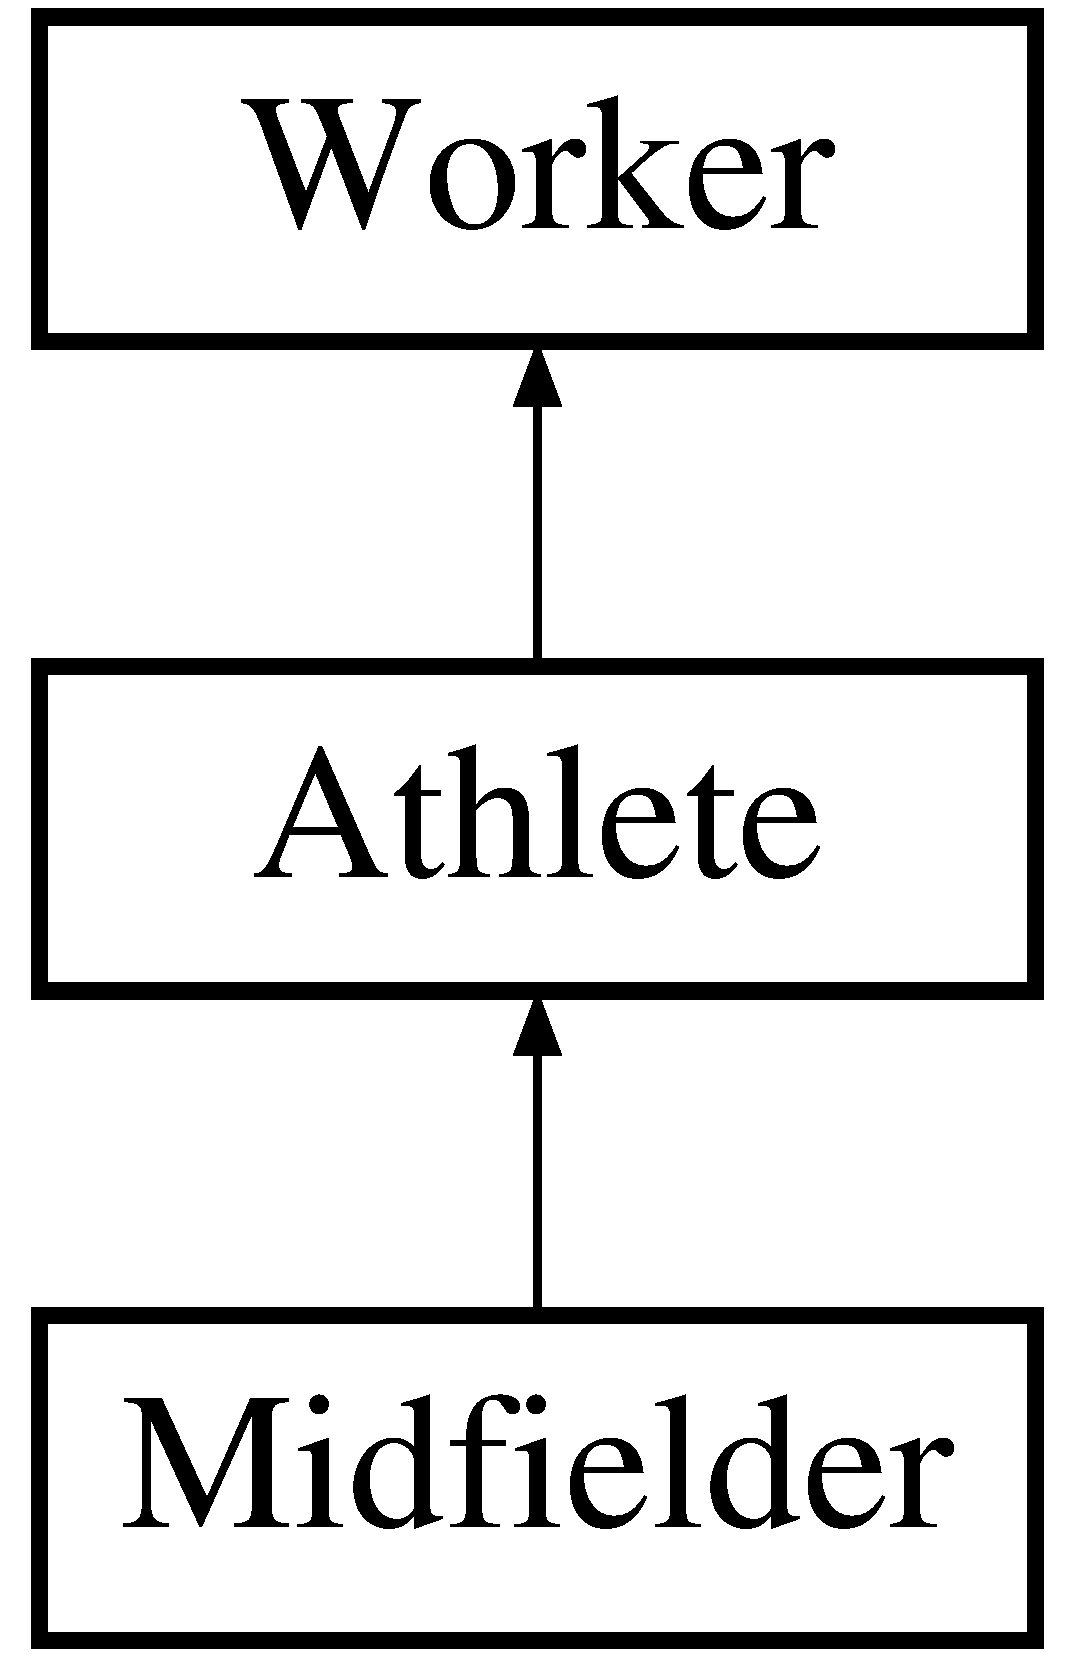
\includegraphics[height=3.000000cm]{class_midfielder}
\end{center}
\end{figure}
\subsection*{Public Member Functions}
\begin{DoxyCompactItemize}
\item 
\hyperlink{class_midfielder_a267913d73597a780ad523d49aadea2f0}{Midfielder} (string \hyperlink{class_worker_a66cf57341253a31e418cf8abad59ffb1}{name}, \hyperlink{class_date}{Date} \hyperlink{class_worker_a3c1845f40a084b471750a787a87614dd}{birthdate}, unsigned int \hyperlink{class_worker_adfafba55f967994f4595bd914bbba127}{civil\+ID}, unsigned char \hyperlink{class_athlete_a80a64bb1d5c943aaa7ca152d596d9914}{height}, unsigned int \hyperlink{class_worker_afc39287cd510977cfe7697ed2c86b2ca}{id}=0)
\item 
\hyperlink{class_midfielder_abab63a71a619509011b23eb3e11e099b}{Midfielder} (string \&new\+MF)
\item 
\hyperlink{class_midfielder_ae0d6c23126b9c08ea3c3a58222d4118f}{$\sim$\+Midfielder} ()
\begin{DoxyCompactList}\small\item\em Destructor. \end{DoxyCompactList}\item 
unsigned int \hyperlink{class_midfielder_ac55e51de4a6544c30ef2471b6c160d2b}{get\+ID} () const
\item 
\hyperlink{class_info}{Info} $\ast$ \hyperlink{class_midfielder_a18c2c163951dd942685950ac562f3b24}{get\+Info} () const
\item 
void \hyperlink{class_midfielder_aca69e728b57110b3f34de94556465c0a}{add\+Info} (\hyperlink{class_info}{Info} $\ast$more\+Info)
\end{DoxyCompactItemize}
\subsection*{Private Attributes}
\begin{DoxyCompactItemize}
\item 
\hyperlink{class_info}{Info} $\ast$ \hyperlink{class_midfielder_aa3b78958ffc35755ca4a06aa642115e5}{general\+Info}
\begin{DoxyCompactList}\small\item\em midfielder\textquotesingle{}s general information. \end{DoxyCompactList}\end{DoxyCompactItemize}
\subsection*{Additional Inherited Members}


\subsection{Constructor \& Destructor Documentation}
\hypertarget{class_midfielder_a267913d73597a780ad523d49aadea2f0}{}\label{class_midfielder_a267913d73597a780ad523d49aadea2f0} 
\index{Midfielder@{Midfielder}!Midfielder@{Midfielder}}
\index{Midfielder@{Midfielder}!Midfielder@{Midfielder}}
\subsubsection{\texorpdfstring{Midfielder()}{Midfielder()}\hspace{0.1cm}{\footnotesize\ttfamily [1/2]}}
{\footnotesize\ttfamily Midfielder\+::\+Midfielder (\begin{DoxyParamCaption}\item[{string}]{name,  }\item[{\hyperlink{class_date}{Date}}]{birthdate,  }\item[{unsigned int}]{civil\+ID,  }\item[{unsigned char}]{height,  }\item[{unsigned int}]{id = {\ttfamily 0} }\end{DoxyParamCaption})}

This is a constructor that creates a new midfielder using his name, birthdate, civil\+ID, height. Id is automatically set \hypertarget{class_midfielder_abab63a71a619509011b23eb3e11e099b}{}\label{class_midfielder_abab63a71a619509011b23eb3e11e099b} 
\index{Midfielder@{Midfielder}!Midfielder@{Midfielder}}
\index{Midfielder@{Midfielder}!Midfielder@{Midfielder}}
\subsubsection{\texorpdfstring{Midfielder()}{Midfielder()}\hspace{0.1cm}{\footnotesize\ttfamily [2/2]}}
{\footnotesize\ttfamily Midfielder\+::\+Midfielder (\begin{DoxyParamCaption}\item[{string \&}]{new\+MF }\end{DoxyParamCaption})}

This is a constructor that creates a new midfielder using his midfield position passed by reference \hypertarget{class_midfielder_ae0d6c23126b9c08ea3c3a58222d4118f}{}\label{class_midfielder_ae0d6c23126b9c08ea3c3a58222d4118f} 
\index{Midfielder@{Midfielder}!````~Midfielder@{$\sim$\+Midfielder}}
\index{````~Midfielder@{$\sim$\+Midfielder}!Midfielder@{Midfielder}}
\subsubsection{\texorpdfstring{$\sim$\+Midfielder()}{~Midfielder()}}
{\footnotesize\ttfamily Midfielder\+::$\sim$\+Midfielder (\begin{DoxyParamCaption}{ }\end{DoxyParamCaption})}



Destructor. 

Luís, 20/11/2016. 

\subsection{Member Function Documentation}
\hypertarget{class_midfielder_aca69e728b57110b3f34de94556465c0a}{}\label{class_midfielder_aca69e728b57110b3f34de94556465c0a} 
\index{Midfielder@{Midfielder}!add\+Info@{add\+Info}}
\index{add\+Info@{add\+Info}!Midfielder@{Midfielder}}
\subsubsection{\texorpdfstring{add\+Info()}{addInfo()}}
{\footnotesize\ttfamily void Midfielder\+::add\+Info (\begin{DoxyParamCaption}\item[{\hyperlink{class_info}{Info} $\ast$}]{more\+Info }\end{DoxyParamCaption})\hspace{0.3cm}{\ttfamily [virtual]}}

This is a method that adds information to the midfielder 

Reimplemented from \hyperlink{class_worker_ad54db262f7473cc729c371dd54e292eb}{Worker}.

\hypertarget{class_midfielder_ac55e51de4a6544c30ef2471b6c160d2b}{}\label{class_midfielder_ac55e51de4a6544c30ef2471b6c160d2b} 
\index{Midfielder@{Midfielder}!get\+ID@{get\+ID}}
\index{get\+ID@{get\+ID}!Midfielder@{Midfielder}}
\subsubsection{\texorpdfstring{get\+I\+D()}{getID()}}
{\footnotesize\ttfamily unsigned int Midfielder\+::get\+ID (\begin{DoxyParamCaption}{ }\end{DoxyParamCaption}) const\hspace{0.3cm}{\ttfamily [virtual]}}

This is a method that gets the midfielder\textquotesingle{}s id 

Implements \hyperlink{class_worker_a8b3e221c4a1ebd12ade03ee9b9c86182}{Worker}.

\hypertarget{class_midfielder_a18c2c163951dd942685950ac562f3b24}{}\label{class_midfielder_a18c2c163951dd942685950ac562f3b24} 
\index{Midfielder@{Midfielder}!get\+Info@{get\+Info}}
\index{get\+Info@{get\+Info}!Midfielder@{Midfielder}}
\subsubsection{\texorpdfstring{get\+Info()}{getInfo()}}
{\footnotesize\ttfamily \hyperlink{class_info}{Info} $\ast$ Midfielder\+::get\+Info (\begin{DoxyParamCaption}{ }\end{DoxyParamCaption}) const\hspace{0.3cm}{\ttfamily [virtual]}}

This is a method that gets the midfielder\textquotesingle{}s performance information 

Reimplemented from \hyperlink{class_worker_a95a4f7c750644937859b8e14515a480e}{Worker}.



\subsection{Member Data Documentation}
\hypertarget{class_midfielder_aa3b78958ffc35755ca4a06aa642115e5}{}\label{class_midfielder_aa3b78958ffc35755ca4a06aa642115e5} 
\index{Midfielder@{Midfielder}!general\+Info@{general\+Info}}
\index{general\+Info@{general\+Info}!Midfielder@{Midfielder}}
\subsubsection{\texorpdfstring{general\+Info}{generalInfo}}
{\footnotesize\ttfamily \hyperlink{class_info}{Info}$\ast$ Midfielder\+::general\+Info\hspace{0.3cm}{\ttfamily [private]}}



midfielder\textquotesingle{}s general information. 



The documentation for this class was generated from the following files\+:\begin{DoxyCompactItemize}
\item 
\hyperlink{_midfielder_8hpp}{Midfielder.\+hpp}\item 
\hyperlink{_midfielder_8cpp}{Midfielder.\+cpp}\end{DoxyCompactItemize}

\hypertarget{class_season}{}\section{Season Class Reference}
\label{class_season}\index{Season@{Season}}


A season.  




{\ttfamily \#include $<$Season.\+hpp$>$}

\subsection*{Public Member Functions}
\begin{DoxyCompactItemize}
\item 
\hyperlink{class_season_aaafaba60ff94d4c85799fcf788ce8eb3}{Season} (unsigned int \hyperlink{class_season_a804663f60306c492542be36f23e20022}{year}, vector$<$ \hyperlink{class_level}{Level} $\ast$$>$ levels\+Vector)
\begin{DoxyCompactList}\small\item\em Constructor. \end{DoxyCompactList}\item 
\hyperlink{class_season_a2e189a58f91fa3718bf2c6234e3b56c3}{Season} (string \hyperlink{class_season_a41002efa6b5ed6a84cf321ca617668eb}{season\+Name}, \hyperlink{class_club}{Club} $\ast$parent\+Club)
\begin{DoxyCompactList}\small\item\em Constructor. \end{DoxyCompactList}\item 
unsigned int \hyperlink{class_season_a437263c3d5536555227adc5b096aa1e1}{get\+Year} () const
\begin{DoxyCompactList}\small\item\em Gets the year. \end{DoxyCompactList}\item 
vector$<$ \hyperlink{class_level}{Level} $\ast$ $>$ \hyperlink{class_season_abedd416fd2c01eb45d1b6c18d3a7a8d0}{get\+Levels} () const
\begin{DoxyCompactList}\small\item\em Gets the levels. \end{DoxyCompactList}\item 
string \hyperlink{class_season_a6fea0a2e3e978a9793fd29e5d879547e}{get\+Path\+To\+Season\+Folder} () const
\begin{DoxyCompactList}\small\item\em Gets path to season folder. \end{DoxyCompactList}\item 
string \hyperlink{class_season_a26e74348cf0105301a3f18edf2284c32}{get\+Season\+Name} () const
\begin{DoxyCompactList}\small\item\em Gets season name. \end{DoxyCompactList}\item 
\hyperlink{class_date}{Date} \hyperlink{class_season_a0707e2e1c277e58f93936c6e211d6ddf}{get\+Initial\+Date} () const
\begin{DoxyCompactList}\small\item\em Gets initial date. \end{DoxyCompactList}\item 
\hyperlink{class_date}{Date} \hyperlink{class_season_a4ed31ffa307d193ba972c6c81b388ba6}{get\+End\+Date} () const
\begin{DoxyCompactList}\small\item\em Gets end date. \end{DoxyCompactList}\end{DoxyCompactItemize}
\subsection*{Private Member Functions}
\begin{DoxyCompactItemize}
\item 
void \hyperlink{class_season_ada58c4b8942d26fd81624e709c8c93b7}{set\+Date\+Interval} ()
\begin{DoxyCompactList}\small\item\em Sets date interval. \end{DoxyCompactList}\end{DoxyCompactItemize}
\subsection*{Private Attributes}
\begin{DoxyCompactItemize}
\item 
unsigned int \hyperlink{class_season_a804663f60306c492542be36f23e20022}{year}
\begin{DoxyCompactList}\small\item\em The year. \end{DoxyCompactList}\item 
\hyperlink{class_date}{Date} \hyperlink{class_season_a509b94f8c80eb1a5f77a72a28dd2561f}{initial\+Date}
\begin{DoxyCompactList}\small\item\em The initial date. \end{DoxyCompactList}\item 
\hyperlink{class_date}{Date} \hyperlink{class_season_a1d00aa2551bb9cf2b55d2cd7c2978311}{end\+Date}
\begin{DoxyCompactList}\small\item\em The end date. \end{DoxyCompactList}\item 
vector$<$ \hyperlink{class_level}{Level} $\ast$ $>$ \hyperlink{class_season_a6a9827750bcc35501396c5a791574f08}{levels}
\begin{DoxyCompactList}\small\item\em The levels. \end{DoxyCompactList}\item 
string \hyperlink{class_season_a739e641c676a73d3d2a3f77867c9df71}{path\+To\+Season\+Folder}
\begin{DoxyCompactList}\small\item\em Pathname of the path to season folder. \end{DoxyCompactList}\item 
string \hyperlink{class_season_a41002efa6b5ed6a84cf321ca617668eb}{season\+Name}
\begin{DoxyCompactList}\small\item\em Name of the season. \end{DoxyCompactList}\end{DoxyCompactItemize}


\subsection{Detailed Description}
A season. 

Lu�s, 20/11/2016. 

\subsection{Constructor \& Destructor Documentation}
\hypertarget{class_season_aaafaba60ff94d4c85799fcf788ce8eb3}{}\label{class_season_aaafaba60ff94d4c85799fcf788ce8eb3} 
\index{Season@{Season}!Season@{Season}}
\index{Season@{Season}!Season@{Season}}
\subsubsection{\texorpdfstring{Season()}{Season()}\hspace{0.1cm}{\footnotesize\ttfamily [1/2]}}
{\footnotesize\ttfamily Season\+::\+Season (\begin{DoxyParamCaption}\item[{unsigned int}]{year,  }\item[{vector$<$ \hyperlink{class_level}{Level} $\ast$$>$}]{levels\+Vector }\end{DoxyParamCaption})}



Constructor. 

Lu�s, 20/11/2016. 


\begin{DoxyParams}{Parameters}
{\em year} & The year. \\
\hline
{\em levels\+Vector} & \mbox{[}in,out\mbox{]} If non-\/null, the levels vector. \\
\hline
\end{DoxyParams}
\hypertarget{class_season_a2e189a58f91fa3718bf2c6234e3b56c3}{}\label{class_season_a2e189a58f91fa3718bf2c6234e3b56c3} 
\index{Season@{Season}!Season@{Season}}
\index{Season@{Season}!Season@{Season}}
\subsubsection{\texorpdfstring{Season()}{Season()}\hspace{0.1cm}{\footnotesize\ttfamily [2/2]}}
{\footnotesize\ttfamily Season\+::\+Season (\begin{DoxyParamCaption}\item[{string}]{season\+Name,  }\item[{\hyperlink{class_club}{Club} $\ast$}]{parent\+Club }\end{DoxyParamCaption})}



Constructor. 

Lu�s, 20/11/2016. 


\begin{DoxyParams}{Parameters}
{\em season\+Name} & Name of the season. \\
\hline
{\em parent\+Club} & \mbox{[}in,out\mbox{]} If non-\/null, the parent club. \\
\hline
\end{DoxyParams}


\subsection{Member Function Documentation}
\hypertarget{class_season_a4ed31ffa307d193ba972c6c81b388ba6}{}\label{class_season_a4ed31ffa307d193ba972c6c81b388ba6} 
\index{Season@{Season}!get\+End\+Date@{get\+End\+Date}}
\index{get\+End\+Date@{get\+End\+Date}!Season@{Season}}
\subsubsection{\texorpdfstring{get\+End\+Date()}{getEndDate()}}
{\footnotesize\ttfamily \hyperlink{class_date}{Date} Season\+::get\+End\+Date (\begin{DoxyParamCaption}{ }\end{DoxyParamCaption}) const}



Gets end date. 

Lu�s, 20/11/2016. 

\begin{DoxyReturn}{Returns}
The end date. 
\end{DoxyReturn}
\hypertarget{class_season_a0707e2e1c277e58f93936c6e211d6ddf}{}\label{class_season_a0707e2e1c277e58f93936c6e211d6ddf} 
\index{Season@{Season}!get\+Initial\+Date@{get\+Initial\+Date}}
\index{get\+Initial\+Date@{get\+Initial\+Date}!Season@{Season}}
\subsubsection{\texorpdfstring{get\+Initial\+Date()}{getInitialDate()}}
{\footnotesize\ttfamily \hyperlink{class_date}{Date} Season\+::get\+Initial\+Date (\begin{DoxyParamCaption}{ }\end{DoxyParamCaption}) const}



Gets initial date. 

Lu�s, 20/11/2016. 

\begin{DoxyReturn}{Returns}
The initial date. 
\end{DoxyReturn}
\hypertarget{class_season_abedd416fd2c01eb45d1b6c18d3a7a8d0}{}\label{class_season_abedd416fd2c01eb45d1b6c18d3a7a8d0} 
\index{Season@{Season}!get\+Levels@{get\+Levels}}
\index{get\+Levels@{get\+Levels}!Season@{Season}}
\subsubsection{\texorpdfstring{get\+Levels()}{getLevels()}}
{\footnotesize\ttfamily vector$<$ \hyperlink{class_level}{Level} $\ast$ $>$ Season\+::get\+Levels (\begin{DoxyParamCaption}{ }\end{DoxyParamCaption}) const}



Gets the levels. 

Lu�s, 20/11/2016. 

\begin{DoxyReturn}{Returns}
Null if it fails, else the levels. 
\end{DoxyReturn}
\hypertarget{class_season_a6fea0a2e3e978a9793fd29e5d879547e}{}\label{class_season_a6fea0a2e3e978a9793fd29e5d879547e} 
\index{Season@{Season}!get\+Path\+To\+Season\+Folder@{get\+Path\+To\+Season\+Folder}}
\index{get\+Path\+To\+Season\+Folder@{get\+Path\+To\+Season\+Folder}!Season@{Season}}
\subsubsection{\texorpdfstring{get\+Path\+To\+Season\+Folder()}{getPathToSeasonFolder()}}
{\footnotesize\ttfamily string Season\+::get\+Path\+To\+Season\+Folder (\begin{DoxyParamCaption}{ }\end{DoxyParamCaption}) const}



Gets path to season folder. 

Lu�s, 20/11/2016. 

\begin{DoxyReturn}{Returns}
The path to season folder. 
\end{DoxyReturn}
\hypertarget{class_season_a26e74348cf0105301a3f18edf2284c32}{}\label{class_season_a26e74348cf0105301a3f18edf2284c32} 
\index{Season@{Season}!get\+Season\+Name@{get\+Season\+Name}}
\index{get\+Season\+Name@{get\+Season\+Name}!Season@{Season}}
\subsubsection{\texorpdfstring{get\+Season\+Name()}{getSeasonName()}}
{\footnotesize\ttfamily string Season\+::get\+Season\+Name (\begin{DoxyParamCaption}{ }\end{DoxyParamCaption}) const}



Gets season name. 

Lu�s, 20/11/2016. 

\begin{DoxyReturn}{Returns}
The season name. 
\end{DoxyReturn}
\hypertarget{class_season_a437263c3d5536555227adc5b096aa1e1}{}\label{class_season_a437263c3d5536555227adc5b096aa1e1} 
\index{Season@{Season}!get\+Year@{get\+Year}}
\index{get\+Year@{get\+Year}!Season@{Season}}
\subsubsection{\texorpdfstring{get\+Year()}{getYear()}}
{\footnotesize\ttfamily unsigned int Season\+::get\+Year (\begin{DoxyParamCaption}{ }\end{DoxyParamCaption}) const}



Gets the year. 

Lu�s, 20/11/2016. 

\begin{DoxyReturn}{Returns}
The year. 
\end{DoxyReturn}
\hypertarget{class_season_ada58c4b8942d26fd81624e709c8c93b7}{}\label{class_season_ada58c4b8942d26fd81624e709c8c93b7} 
\index{Season@{Season}!set\+Date\+Interval@{set\+Date\+Interval}}
\index{set\+Date\+Interval@{set\+Date\+Interval}!Season@{Season}}
\subsubsection{\texorpdfstring{set\+Date\+Interval()}{setDateInterval()}}
{\footnotesize\ttfamily void Season\+::set\+Date\+Interval (\begin{DoxyParamCaption}{ }\end{DoxyParamCaption})\hspace{0.3cm}{\ttfamily [private]}}



Sets date interval. 

Lu�s, 20/11/2016. 

\subsection{Member Data Documentation}
\hypertarget{class_season_a1d00aa2551bb9cf2b55d2cd7c2978311}{}\label{class_season_a1d00aa2551bb9cf2b55d2cd7c2978311} 
\index{Season@{Season}!end\+Date@{end\+Date}}
\index{end\+Date@{end\+Date}!Season@{Season}}
\subsubsection{\texorpdfstring{end\+Date}{endDate}}
{\footnotesize\ttfamily \hyperlink{class_date}{Date} Season\+::end\+Date\hspace{0.3cm}{\ttfamily [private]}}



The end date. 

\hypertarget{class_season_a509b94f8c80eb1a5f77a72a28dd2561f}{}\label{class_season_a509b94f8c80eb1a5f77a72a28dd2561f} 
\index{Season@{Season}!initial\+Date@{initial\+Date}}
\index{initial\+Date@{initial\+Date}!Season@{Season}}
\subsubsection{\texorpdfstring{initial\+Date}{initialDate}}
{\footnotesize\ttfamily \hyperlink{class_date}{Date} Season\+::initial\+Date\hspace{0.3cm}{\ttfamily [private]}}



The initial date. 

\hypertarget{class_season_a6a9827750bcc35501396c5a791574f08}{}\label{class_season_a6a9827750bcc35501396c5a791574f08} 
\index{Season@{Season}!levels@{levels}}
\index{levels@{levels}!Season@{Season}}
\subsubsection{\texorpdfstring{levels}{levels}}
{\footnotesize\ttfamily vector$<$\hyperlink{class_level}{Level}$\ast$$>$ Season\+::levels\hspace{0.3cm}{\ttfamily [private]}}



The levels. 

\hypertarget{class_season_a739e641c676a73d3d2a3f77867c9df71}{}\label{class_season_a739e641c676a73d3d2a3f77867c9df71} 
\index{Season@{Season}!path\+To\+Season\+Folder@{path\+To\+Season\+Folder}}
\index{path\+To\+Season\+Folder@{path\+To\+Season\+Folder}!Season@{Season}}
\subsubsection{\texorpdfstring{path\+To\+Season\+Folder}{pathToSeasonFolder}}
{\footnotesize\ttfamily string Season\+::path\+To\+Season\+Folder\hspace{0.3cm}{\ttfamily [private]}}



Pathname of the path to season folder. 

\hypertarget{class_season_a41002efa6b5ed6a84cf321ca617668eb}{}\label{class_season_a41002efa6b5ed6a84cf321ca617668eb} 
\index{Season@{Season}!season\+Name@{season\+Name}}
\index{season\+Name@{season\+Name}!Season@{Season}}
\subsubsection{\texorpdfstring{season\+Name}{seasonName}}
{\footnotesize\ttfamily string Season\+::season\+Name\hspace{0.3cm}{\ttfamily [private]}}



Name of the season. 

\hypertarget{class_season_a804663f60306c492542be36f23e20022}{}\label{class_season_a804663f60306c492542be36f23e20022} 
\index{Season@{Season}!year@{year}}
\index{year@{year}!Season@{Season}}
\subsubsection{\texorpdfstring{year}{year}}
{\footnotesize\ttfamily unsigned int Season\+::year\hspace{0.3cm}{\ttfamily [private]}}



The year. 



The documentation for this class was generated from the following files\+:\begin{DoxyCompactItemize}
\item 
\hyperlink{_season_8hpp}{Season.\+hpp}\item 
\hyperlink{_season_8cpp}{Season.\+cpp}\end{DoxyCompactItemize}

\hypertarget{class_sort_training}{}\section{Sort\+Training Class Reference}
\label{class_sort_training}\index{Sort\+Training@{Sort\+Training}}


A sort training.  




{\ttfamily \#include $<$Training.\+hpp$>$}

\subsection*{Public Member Functions}
\begin{DoxyCompactItemize}
\item 
\hyperlink{class_sort_training_adf058e5b7c1de349a4d07206401fd865}{Sort\+Training} (\hyperlink{_training_8hpp_aa44c715f606358e721f7911b15a1cfc5}{Sort\+Criteria} \hyperlink{class_sort_training_adad567b222d6d5c2799d58ce9fce4682}{criteria}, \hyperlink{_training_8hpp_ad9be72f666a31b4318bbc8e8a16a9472}{Sort\+Order} \hyperlink{class_sort_training_a813c7ada10d981e1cc468bac20410460}{order})
\begin{DoxyCompactList}\small\item\em Constructor that sorts a vector of trainings. \end{DoxyCompactList}\item 
bool \hyperlink{class_sort_training_a20fcf9d5d652278d080239edebabd61e}{operator()} (\hyperlink{class_training}{Training} $\ast$t1, \hyperlink{class_training}{Training} $\ast$t2)
\begin{DoxyCompactList}\small\item\em Function call operator. \end{DoxyCompactList}\end{DoxyCompactItemize}
\subsection*{Private Attributes}
\begin{DoxyCompactItemize}
\item 
\hyperlink{_training_8hpp_aa44c715f606358e721f7911b15a1cfc5}{Sort\+Criteria} \hyperlink{class_sort_training_adad567b222d6d5c2799d58ce9fce4682}{criteria}
\begin{DoxyCompactList}\small\item\em The criteria. \end{DoxyCompactList}\item 
\hyperlink{_training_8hpp_ad9be72f666a31b4318bbc8e8a16a9472}{Sort\+Order} \hyperlink{class_sort_training_a813c7ada10d981e1cc468bac20410460}{order}
\begin{DoxyCompactList}\small\item\em The order. \end{DoxyCompactList}\end{DoxyCompactItemize}


\subsection{Detailed Description}
A sort training. 

Lu�s, 20/11/2016. 

\subsection{Constructor \& Destructor Documentation}
\hypertarget{class_sort_training_adf058e5b7c1de349a4d07206401fd865}{}\label{class_sort_training_adf058e5b7c1de349a4d07206401fd865} 
\index{Sort\+Training@{Sort\+Training}!Sort\+Training@{Sort\+Training}}
\index{Sort\+Training@{Sort\+Training}!Sort\+Training@{Sort\+Training}}
\subsubsection{\texorpdfstring{Sort\+Training()}{SortTraining()}}
{\footnotesize\ttfamily Sort\+Training\+::\+Sort\+Training (\begin{DoxyParamCaption}\item[{\hyperlink{_training_8hpp_aa44c715f606358e721f7911b15a1cfc5}{Sort\+Criteria}}]{criteria,  }\item[{\hyperlink{_training_8hpp_ad9be72f666a31b4318bbc8e8a16a9472}{Sort\+Order}}]{order }\end{DoxyParamCaption})}



Constructor that sorts a vector of trainings. 

Lu�s, 20/11/2016. 


\begin{DoxyParams}{Parameters}
{\em criteria} & The criteria. \\
\hline
{\em order} & The order. \\
\hline
\end{DoxyParams}


\subsection{Member Function Documentation}
\hypertarget{class_sort_training_a20fcf9d5d652278d080239edebabd61e}{}\label{class_sort_training_a20fcf9d5d652278d080239edebabd61e} 
\index{Sort\+Training@{Sort\+Training}!operator()@{operator()}}
\index{operator()@{operator()}!Sort\+Training@{Sort\+Training}}
\subsubsection{\texorpdfstring{operator()()}{operator()()}}
{\footnotesize\ttfamily bool Sort\+Training\+::operator() (\begin{DoxyParamCaption}\item[{\hyperlink{class_training}{Training} $\ast$}]{t1,  }\item[{\hyperlink{class_training}{Training} $\ast$}]{t2 }\end{DoxyParamCaption})}



Function call operator. 

Lu�s, 20/11/2016. 


\begin{DoxyParams}{Parameters}
{\em t1} & \mbox{[}in,out\mbox{]} If non-\/null, the first \hyperlink{class_training}{Training}. \\
\hline
{\em t2} & \mbox{[}in,out\mbox{]} If non-\/null, the last \hyperlink{class_training}{Training}. \\
\hline
\end{DoxyParams}


\begin{DoxyReturn}{Returns}
The result of the operation. 
\end{DoxyReturn}


\subsection{Member Data Documentation}
\hypertarget{class_sort_training_adad567b222d6d5c2799d58ce9fce4682}{}\label{class_sort_training_adad567b222d6d5c2799d58ce9fce4682} 
\index{Sort\+Training@{Sort\+Training}!criteria@{criteria}}
\index{criteria@{criteria}!Sort\+Training@{Sort\+Training}}
\subsubsection{\texorpdfstring{criteria}{criteria}}
{\footnotesize\ttfamily \hyperlink{_training_8hpp_aa44c715f606358e721f7911b15a1cfc5}{Sort\+Criteria} Sort\+Training\+::criteria\hspace{0.3cm}{\ttfamily [private]}}



The criteria. 

\hypertarget{class_sort_training_a813c7ada10d981e1cc468bac20410460}{}\label{class_sort_training_a813c7ada10d981e1cc468bac20410460} 
\index{Sort\+Training@{Sort\+Training}!order@{order}}
\index{order@{order}!Sort\+Training@{Sort\+Training}}
\subsubsection{\texorpdfstring{order}{order}}
{\footnotesize\ttfamily \hyperlink{_training_8hpp_ad9be72f666a31b4318bbc8e8a16a9472}{Sort\+Order} Sort\+Training\+::order\hspace{0.3cm}{\ttfamily [private]}}



The order. 



The documentation for this class was generated from the following files\+:\begin{DoxyCompactItemize}
\item 
\hyperlink{_training_8hpp}{Training.\+hpp}\item 
\hyperlink{_training_8cpp}{Training.\+cpp}\end{DoxyCompactItemize}

\hypertarget{class_table}{}\section{Table Class Reference}
\label{class_table}\index{Table@{Table}}


{\ttfamily \#include $<$Utils.\+hpp$>$}

\subsection*{Public Member Functions}
\begin{DoxyCompactItemize}
\item 
\hyperlink{class_table_a80b23f471aa594c4d1a1db51a22fb6c4}{Table} (vector$<$ string $>$ components, unsigned int indentacao=0)
\item 
\hyperlink{class_table_a65aecaa868a14218cbecb86437f996c1}{Table} (vector$<$ string $>$ components, vector$<$ int $>$ spaces\+For\+Column, unsigned int indentacao=0)
\item 
\hyperlink{class_table_a9abee52d5b062c43f79bfe55c67b7759}{Table} (vector$<$ vector$<$ string $>$$>$ \hyperlink{class_table_a9052c218f9eae23950459720e8069e62}{table\+Vector}, vector$<$ bool $>$ \hyperlink{class_table_a733288d34b5fd55085572f212fbe0260}{blocks}, vector$<$ int $>$ spaces\+For\+Column, unsigned int indentacao=0)
\item 
\hyperlink{class_table_a49c13a4307cb192d0a449f948dda66e2}{Table} (vector$<$ vector$<$ string $>$$>$ \hyperlink{class_table_a9052c218f9eae23950459720e8069e62}{table\+Vector}, unsigned int indentation)
\item 
void \hyperlink{class_table_a3c9712fbea1a7101e5aa28adc42d50b5}{format\+Table} (char internal\+Char, char limiting\+Char, vector$<$ int $>$ spaces\+For\+Column, unsigned int indentacao\+FT=0)
\item 
vector$<$ int $>$ \hyperlink{class_table_ab6541bd5783a13f8958e7def259ad844}{get\+Colums\+Width} () const
\item 
unsigned int \hyperlink{class_table_aa6fd97bbceb82d9acddf1858f3dbfc14}{get\+Indentacao} () const
\item 
vector$<$ vector$<$ string $>$ $>$ \hyperlink{class_table_a4a3ecdc1ad22d0dadd116af3cda3a74d}{get\+Table\+Vector} () const
\item 
vector$<$ bool $>$ \hyperlink{class_table_aeefe34b1ca9fa483b3605f9d6adbfdb5}{get\+Blocks} () const
\item 
string \hyperlink{class_table_a695b8d8f464194e26bcf23e07cd216bd}{get\+Stream} () const
\item 
void \hyperlink{class_table_a8d1739ca805a00714d030303124c2927}{add\+New\+Line} (vector$<$ string $>$ components)
\item 
void \hyperlink{class_table_ac1fcf6cb33298c4fbfa5457e0b276738}{add\+Data\+In\+Same\+Line} (vector$<$ string $>$ components)
\item 
void \hyperlink{class_table_aee12cc19eef2f8d152d92c6c92011207}{adjust\+Columns\+Size} (vector$<$ int $>$ spaspaces\+For\+Column)
\end{DoxyCompactItemize}
\subsection*{Public Attributes}
\begin{DoxyCompactItemize}
\item 
stringstream \hyperlink{class_table_a9df4c1c33927ef0b7cd474d4420a7278}{table\+Stream}
\end{DoxyCompactItemize}
\subsection*{Private Attributes}
\begin{DoxyCompactItemize}
\item 
vector$<$ vector$<$ string $>$ $>$ \hyperlink{class_table_a9052c218f9eae23950459720e8069e62}{table\+Vector}
\item 
vector$<$ bool $>$ \hyperlink{class_table_a733288d34b5fd55085572f212fbe0260}{blocks}
\item 
unsigned int \hyperlink{class_table_a88a6ec978fe9116bbfed4e7aa066b5e2}{num\+Columns}
\item 
unsigned int \hyperlink{class_table_a0e4ed290246197725eee0c0a266b85d2}{num\+Lines}
\item 
vector$<$ int $>$ \hyperlink{class_table_a36e32fdefca7b32f938d0029496c4238}{columns\+Width}
\item 
vector$<$ string $>$ \hyperlink{class_table_a2e6a2cba72cb9975758d05507ded659e}{last\+Line\+Components}
\item 
unsigned int \hyperlink{class_table_a4e5eecbb3e6363585df871429381f433}{indent}
\end{DoxyCompactItemize}
\subsection*{Friends}
\begin{DoxyCompactItemize}
\item 
ostream \& \hyperlink{class_table_af5e0f2c2e64aa1dc084c36859c54a289}{operator$<$$<$} (ostream \&out, const \hyperlink{class_table}{Table} \&table)
\end{DoxyCompactItemize}


\subsection{Constructor \& Destructor Documentation}
\hypertarget{class_table_a80b23f471aa594c4d1a1db51a22fb6c4}{}\label{class_table_a80b23f471aa594c4d1a1db51a22fb6c4} 
\index{Table@{Table}!Table@{Table}}
\index{Table@{Table}!Table@{Table}}
\subsubsection{\texorpdfstring{Table()}{Table()}\hspace{0.1cm}{\footnotesize\ttfamily [1/4]}}
{\footnotesize\ttfamily Table\+::\+Table (\begin{DoxyParamCaption}\item[{vector$<$ string $>$}]{components,  }\item[{unsigned int}]{indentacao = {\ttfamily 0} }\end{DoxyParamCaption})}

\hypertarget{class_table_a65aecaa868a14218cbecb86437f996c1}{}\label{class_table_a65aecaa868a14218cbecb86437f996c1} 
\index{Table@{Table}!Table@{Table}}
\index{Table@{Table}!Table@{Table}}
\subsubsection{\texorpdfstring{Table()}{Table()}\hspace{0.1cm}{\footnotesize\ttfamily [2/4]}}
{\footnotesize\ttfamily Table\+::\+Table (\begin{DoxyParamCaption}\item[{vector$<$ string $>$}]{components,  }\item[{vector$<$ int $>$}]{spaces\+For\+Column,  }\item[{unsigned int}]{indentacao = {\ttfamily 0} }\end{DoxyParamCaption})}

\hypertarget{class_table_a9abee52d5b062c43f79bfe55c67b7759}{}\label{class_table_a9abee52d5b062c43f79bfe55c67b7759} 
\index{Table@{Table}!Table@{Table}}
\index{Table@{Table}!Table@{Table}}
\subsubsection{\texorpdfstring{Table()}{Table()}\hspace{0.1cm}{\footnotesize\ttfamily [3/4]}}
{\footnotesize\ttfamily Table\+::\+Table (\begin{DoxyParamCaption}\item[{vector$<$ vector$<$ string $>$$>$}]{table\+Vector,  }\item[{vector$<$ bool $>$}]{blocks,  }\item[{vector$<$ int $>$}]{spaces\+For\+Column,  }\item[{unsigned int}]{indentacao = {\ttfamily 0} }\end{DoxyParamCaption})}

\hypertarget{class_table_a49c13a4307cb192d0a449f948dda66e2}{}\label{class_table_a49c13a4307cb192d0a449f948dda66e2} 
\index{Table@{Table}!Table@{Table}}
\index{Table@{Table}!Table@{Table}}
\subsubsection{\texorpdfstring{Table()}{Table()}\hspace{0.1cm}{\footnotesize\ttfamily [4/4]}}
{\footnotesize\ttfamily Table\+::\+Table (\begin{DoxyParamCaption}\item[{vector$<$ vector$<$ string $>$$>$}]{table\+Vector,  }\item[{unsigned int}]{indentation }\end{DoxyParamCaption})}



\subsection{Member Function Documentation}
\hypertarget{class_table_ac1fcf6cb33298c4fbfa5457e0b276738}{}\label{class_table_ac1fcf6cb33298c4fbfa5457e0b276738} 
\index{Table@{Table}!add\+Data\+In\+Same\+Line@{add\+Data\+In\+Same\+Line}}
\index{add\+Data\+In\+Same\+Line@{add\+Data\+In\+Same\+Line}!Table@{Table}}
\subsubsection{\texorpdfstring{add\+Data\+In\+Same\+Line()}{addDataInSameLine()}}
{\footnotesize\ttfamily void Table\+::add\+Data\+In\+Same\+Line (\begin{DoxyParamCaption}\item[{vector$<$ string $>$}]{components }\end{DoxyParamCaption})}

\hypertarget{class_table_a8d1739ca805a00714d030303124c2927}{}\label{class_table_a8d1739ca805a00714d030303124c2927} 
\index{Table@{Table}!add\+New\+Line@{add\+New\+Line}}
\index{add\+New\+Line@{add\+New\+Line}!Table@{Table}}
\subsubsection{\texorpdfstring{add\+New\+Line()}{addNewLine()}}
{\footnotesize\ttfamily void Table\+::add\+New\+Line (\begin{DoxyParamCaption}\item[{vector$<$ string $>$}]{components }\end{DoxyParamCaption})}

\hypertarget{class_table_aee12cc19eef2f8d152d92c6c92011207}{}\label{class_table_aee12cc19eef2f8d152d92c6c92011207} 
\index{Table@{Table}!adjust\+Columns\+Size@{adjust\+Columns\+Size}}
\index{adjust\+Columns\+Size@{adjust\+Columns\+Size}!Table@{Table}}
\subsubsection{\texorpdfstring{adjust\+Columns\+Size()}{adjustColumnsSize()}}
{\footnotesize\ttfamily void Table\+::adjust\+Columns\+Size (\begin{DoxyParamCaption}\item[{vector$<$ int $>$}]{spaspaces\+For\+Column }\end{DoxyParamCaption})}

\hypertarget{class_table_a3c9712fbea1a7101e5aa28adc42d50b5}{}\label{class_table_a3c9712fbea1a7101e5aa28adc42d50b5} 
\index{Table@{Table}!format\+Table@{format\+Table}}
\index{format\+Table@{format\+Table}!Table@{Table}}
\subsubsection{\texorpdfstring{format\+Table()}{formatTable()}}
{\footnotesize\ttfamily void Table\+::format\+Table (\begin{DoxyParamCaption}\item[{char}]{internal\+Char,  }\item[{char}]{limiting\+Char,  }\item[{vector$<$ int $>$}]{spaces\+For\+Column,  }\item[{unsigned int}]{indentacao\+FT = {\ttfamily 0} }\end{DoxyParamCaption})}

\hypertarget{class_table_aeefe34b1ca9fa483b3605f9d6adbfdb5}{}\label{class_table_aeefe34b1ca9fa483b3605f9d6adbfdb5} 
\index{Table@{Table}!get\+Blocks@{get\+Blocks}}
\index{get\+Blocks@{get\+Blocks}!Table@{Table}}
\subsubsection{\texorpdfstring{get\+Blocks()}{getBlocks()}}
{\footnotesize\ttfamily vector$<$ bool $>$ Table\+::get\+Blocks (\begin{DoxyParamCaption}{ }\end{DoxyParamCaption}) const}

\hypertarget{class_table_ab6541bd5783a13f8958e7def259ad844}{}\label{class_table_ab6541bd5783a13f8958e7def259ad844} 
\index{Table@{Table}!get\+Colums\+Width@{get\+Colums\+Width}}
\index{get\+Colums\+Width@{get\+Colums\+Width}!Table@{Table}}
\subsubsection{\texorpdfstring{get\+Colums\+Width()}{getColumsWidth()}}
{\footnotesize\ttfamily vector$<$ int $>$ Table\+::get\+Colums\+Width (\begin{DoxyParamCaption}{ }\end{DoxyParamCaption}) const}

\hypertarget{class_table_aa6fd97bbceb82d9acddf1858f3dbfc14}{}\label{class_table_aa6fd97bbceb82d9acddf1858f3dbfc14} 
\index{Table@{Table}!get\+Indentacao@{get\+Indentacao}}
\index{get\+Indentacao@{get\+Indentacao}!Table@{Table}}
\subsubsection{\texorpdfstring{get\+Indentacao()}{getIndentacao()}}
{\footnotesize\ttfamily unsigned int Table\+::get\+Indentacao (\begin{DoxyParamCaption}{ }\end{DoxyParamCaption}) const}

\hypertarget{class_table_a695b8d8f464194e26bcf23e07cd216bd}{}\label{class_table_a695b8d8f464194e26bcf23e07cd216bd} 
\index{Table@{Table}!get\+Stream@{get\+Stream}}
\index{get\+Stream@{get\+Stream}!Table@{Table}}
\subsubsection{\texorpdfstring{get\+Stream()}{getStream()}}
{\footnotesize\ttfamily string Table\+::get\+Stream (\begin{DoxyParamCaption}{ }\end{DoxyParamCaption}) const}

\hypertarget{class_table_a4a3ecdc1ad22d0dadd116af3cda3a74d}{}\label{class_table_a4a3ecdc1ad22d0dadd116af3cda3a74d} 
\index{Table@{Table}!get\+Table\+Vector@{get\+Table\+Vector}}
\index{get\+Table\+Vector@{get\+Table\+Vector}!Table@{Table}}
\subsubsection{\texorpdfstring{get\+Table\+Vector()}{getTableVector()}}
{\footnotesize\ttfamily vector$<$ vector$<$ string $>$ $>$ Table\+::get\+Table\+Vector (\begin{DoxyParamCaption}{ }\end{DoxyParamCaption}) const}



\subsection{Friends And Related Function Documentation}
\hypertarget{class_table_af5e0f2c2e64aa1dc084c36859c54a289}{}\label{class_table_af5e0f2c2e64aa1dc084c36859c54a289} 
\index{Table@{Table}!operator$<$$<$@{operator$<$$<$}}
\index{operator$<$$<$@{operator$<$$<$}!Table@{Table}}
\subsubsection{\texorpdfstring{operator$<$$<$}{operator<<}}
{\footnotesize\ttfamily ostream\& operator$<$$<$ (\begin{DoxyParamCaption}\item[{ostream \&}]{out,  }\item[{const \hyperlink{class_table}{Table} \&}]{table }\end{DoxyParamCaption})\hspace{0.3cm}{\ttfamily [friend]}}



\subsection{Member Data Documentation}
\hypertarget{class_table_a733288d34b5fd55085572f212fbe0260}{}\label{class_table_a733288d34b5fd55085572f212fbe0260} 
\index{Table@{Table}!blocks@{blocks}}
\index{blocks@{blocks}!Table@{Table}}
\subsubsection{\texorpdfstring{blocks}{blocks}}
{\footnotesize\ttfamily vector$<$bool$>$ Table\+::blocks\hspace{0.3cm}{\ttfamily [private]}}

\hypertarget{class_table_a36e32fdefca7b32f938d0029496c4238}{}\label{class_table_a36e32fdefca7b32f938d0029496c4238} 
\index{Table@{Table}!columns\+Width@{columns\+Width}}
\index{columns\+Width@{columns\+Width}!Table@{Table}}
\subsubsection{\texorpdfstring{columns\+Width}{columnsWidth}}
{\footnotesize\ttfamily vector$<$int$>$ Table\+::columns\+Width\hspace{0.3cm}{\ttfamily [private]}}

\hypertarget{class_table_a4e5eecbb3e6363585df871429381f433}{}\label{class_table_a4e5eecbb3e6363585df871429381f433} 
\index{Table@{Table}!indent@{indent}}
\index{indent@{indent}!Table@{Table}}
\subsubsection{\texorpdfstring{indent}{indent}}
{\footnotesize\ttfamily unsigned int Table\+::indent\hspace{0.3cm}{\ttfamily [private]}}

\hypertarget{class_table_a2e6a2cba72cb9975758d05507ded659e}{}\label{class_table_a2e6a2cba72cb9975758d05507ded659e} 
\index{Table@{Table}!last\+Line\+Components@{last\+Line\+Components}}
\index{last\+Line\+Components@{last\+Line\+Components}!Table@{Table}}
\subsubsection{\texorpdfstring{last\+Line\+Components}{lastLineComponents}}
{\footnotesize\ttfamily vector$<$string$>$ Table\+::last\+Line\+Components\hspace{0.3cm}{\ttfamily [private]}}

\hypertarget{class_table_a88a6ec978fe9116bbfed4e7aa066b5e2}{}\label{class_table_a88a6ec978fe9116bbfed4e7aa066b5e2} 
\index{Table@{Table}!num\+Columns@{num\+Columns}}
\index{num\+Columns@{num\+Columns}!Table@{Table}}
\subsubsection{\texorpdfstring{num\+Columns}{numColumns}}
{\footnotesize\ttfamily unsigned int Table\+::num\+Columns\hspace{0.3cm}{\ttfamily [private]}}

\hypertarget{class_table_a0e4ed290246197725eee0c0a266b85d2}{}\label{class_table_a0e4ed290246197725eee0c0a266b85d2} 
\index{Table@{Table}!num\+Lines@{num\+Lines}}
\index{num\+Lines@{num\+Lines}!Table@{Table}}
\subsubsection{\texorpdfstring{num\+Lines}{numLines}}
{\footnotesize\ttfamily unsigned int Table\+::num\+Lines\hspace{0.3cm}{\ttfamily [private]}}

\hypertarget{class_table_a9df4c1c33927ef0b7cd474d4420a7278}{}\label{class_table_a9df4c1c33927ef0b7cd474d4420a7278} 
\index{Table@{Table}!table\+Stream@{table\+Stream}}
\index{table\+Stream@{table\+Stream}!Table@{Table}}
\subsubsection{\texorpdfstring{table\+Stream}{tableStream}}
{\footnotesize\ttfamily stringstream Table\+::table\+Stream}

\hypertarget{class_table_a9052c218f9eae23950459720e8069e62}{}\label{class_table_a9052c218f9eae23950459720e8069e62} 
\index{Table@{Table}!table\+Vector@{table\+Vector}}
\index{table\+Vector@{table\+Vector}!Table@{Table}}
\subsubsection{\texorpdfstring{table\+Vector}{tableVector}}
{\footnotesize\ttfamily vector$<$vector$<$string$>$ $>$ Table\+::table\+Vector\hspace{0.3cm}{\ttfamily [private]}}



The documentation for this class was generated from the following files\+:\begin{DoxyCompactItemize}
\item 
\hyperlink{_utils_8hpp}{Utils.\+hpp}\item 
\hyperlink{_utils_8cpp}{Utils.\+cpp}\end{DoxyCompactItemize}

\hypertarget{class_tournament}{}\section{Tournament Class Reference}
\label{class_tournament}\index{Tournament@{Tournament}}


A tournament.  




{\ttfamily \#include $<$Tournament.\+hpp$>$}

\subsection*{Public Member Functions}
\begin{DoxyCompactItemize}
\item 
\hyperlink{class_tournament_a65490b32c093ace034b15ec8cbe75795}{Tournament} (\hyperlink{class_date}{Date} \hyperlink{class_tournament_afe5c5994c15194a320914831d05e40fc}{tournament\+Starting\+Date}, \hyperlink{class_date}{Date} \hyperlink{class_tournament_a85027b414ba2ddd7cd513c399588d2a8}{tournament\+Ending\+Date}, vector$<$ string $>$ tournament\+Clubs, \hyperlink{class_club}{Club} $\ast$program\+Club, string \hyperlink{class_tournament_a6d4f678a73d89147d34bb1d0c50cc976}{name}, unsigned int \hyperlink{class_tournament_a15cf54c0cde58d9a29c9700808173a8c}{id}=0)
\begin{DoxyCompactList}\small\item\em Constructor. \end{DoxyCompactList}\item 
\hyperlink{class_tournament_a4d5e4eb2007fb6873b5e4e91f70d565b}{Tournament} (ifstream \&in\+Stream, ifstream \&\hyperlink{class_tournament_a561cd3b82b192558910f85ae1c1f5bea}{tournament\+Tree}, \hyperlink{class_level}{Level} $\ast$tournament\+Level)
\begin{DoxyCompactList}\small\item\em Constructor. \end{DoxyCompactList}\item 
\hyperlink{class_tournament_a3cd15abb3e9599c60ae124fed5a04ee5}{$\sim$\+Tournament} ()
\begin{DoxyCompactList}\small\item\em Destructor. \end{DoxyCompactList}\item 
string \hyperlink{class_tournament_a94cfb5371bd09ab75a50a13ef924ae58}{get\+Name} () const
\begin{DoxyCompactList}\small\item\em Gets the name. \end{DoxyCompactList}\item 
\hyperlink{class_date}{Date} \hyperlink{class_tournament_a30bc0b9edbc862c7318d94199f6a94ee}{get\+Tournament\+Starting\+Date} () const
\begin{DoxyCompactList}\small\item\em Gets tournament starting date. \end{DoxyCompactList}\item 
\hyperlink{class_date}{Date} \hyperlink{class_tournament_adffedf926ee07ba1a18424f71070ad3e}{get\+Tournament\+Ending\+Date} () const
\begin{DoxyCompactList}\small\item\em Gets tournament ending date. \end{DoxyCompactList}\item 
\hyperlink{class_binary_tree}{Binary\+Tree}$<$ \hyperlink{_tournament_8hpp_a59a90f79e961bd9bc490adbf767f7cc4}{node\+Match} $>$ \hyperlink{class_tournament_ada52b0008dc78beee5c64718ce72a9ed}{fill\+Tournament\+Tree} (unsigned int final\+Phase)
\begin{DoxyCompactList}\small\item\em Fill tournament tree. \end{DoxyCompactList}\item 
\hyperlink{_tournament_8hpp_a59a90f79e961bd9bc490adbf767f7cc4}{node\+Match} $\ast$ \hyperlink{class_tournament_af89af84fd12e55685a9693551b6b7652}{find\+Match\+Node} (unsigned int tournament\+Match\+Id)
\begin{DoxyCompactList}\small\item\em Searches for the first match node. \end{DoxyCompactList}\item 
unsigned int \hyperlink{class_tournament_ad5e59e6551498b634e7bd745a7967fc9}{get\+Id} () const
\begin{DoxyCompactList}\small\item\em Gets the identifier. \end{DoxyCompactList}\item 
vector$<$ \hyperlink{class_club}{Club} $\ast$ $>$ \hyperlink{class_tournament_a51a2a85ded44857ab3798c8a9855f5b6}{get\+Tournament\+Clubs} () const
\begin{DoxyCompactList}\small\item\em Gets tournament clubs. \end{DoxyCompactList}\item 
const \hyperlink{class_binary_tree}{Binary\+Tree}$<$ \hyperlink{_tournament_8hpp_a59a90f79e961bd9bc490adbf767f7cc4}{node\+Match} $>$ \& \hyperlink{class_tournament_abeb767d12aab092bf94410e7224cf29b}{get\+Tournament\+Tree} () const
\begin{DoxyCompactList}\small\item\em Gets tournament tree. \end{DoxyCompactList}\item 
vector$<$ vector$<$ string $>$ $>$ \hyperlink{class_tournament_af7b21e0eff39c9ebcba96f1a319d7f67}{get\+Tournament\+Matches} () const
\begin{DoxyCompactList}\small\item\em Gets tournament matches. \end{DoxyCompactList}\item 
void \hyperlink{class_tournament_a8f132d5b00451d7c65eafd3048e29362}{schedule\+Tournament\+Match} (unsigned int tournament\+Match\+Id, \hyperlink{class_date}{Date} match\+Date, unsigned int home\+Team\+Index=0, unsigned int away\+Team\+Index=0)
\begin{DoxyCompactList}\small\item\em Schedule tournament match. \end{DoxyCompactList}\item 
void \hyperlink{class_tournament_adbc7625a6fab79463241834d05fc5bfb}{call\+Up\+Players} (unsigned int tournament\+Match\+Id, vector$<$ unsigned int $>$ match\+Players)
\begin{DoxyCompactList}\small\item\em Call up players. \end{DoxyCompactList}\item 
void \hyperlink{class_tournament_a15948a541a1675213e52381c6a67f51c}{call\+Up\+Players} (unsigned int tournament\+Match\+Id, \hyperlink{class_date}{Date} match\+Date, \hyperlink{class_level}{Level} $\ast$level, vector$<$ unsigned int $>$ match\+Players, unsigned int home\+Team\+Index=0, unsigned int away\+Team\+Index=0)
\begin{DoxyCompactList}\small\item\em Call up players. \end{DoxyCompactList}\item 
void \hyperlink{class_tournament_aa795dcb0ac03da77e9b916d8ef19bd63}{register\+Match} (unsigned int tournament\+Match\+Id, \hyperlink{class_level}{Level} $\ast$level, unsigned int home\+Team\+Score, unsigned int away\+Team\+Score, vector$<$ unsigned int $>$ match\+Players)
\begin{DoxyCompactList}\small\item\em Registers the match. \end{DoxyCompactList}\item 
void \hyperlink{class_tournament_a344a73233eab3d1c2aa1224ec2f3cd5b}{register\+Match} (unsigned int tournament\+Match\+Id, \hyperlink{class_date}{Date} match\+Date, \hyperlink{class_level}{Level} $\ast$level, vector$<$ unsigned int $>$ match\+Players, unsigned int home\+Team\+Score=0, unsigned int away\+Team\+Score=0, unsigned int home\+Team\+Index=0, unsigned int away\+Team\+Index=0)
\begin{DoxyCompactList}\small\item\em Registers the match. \end{DoxyCompactList}\item 
void \hyperlink{class_tournament_a98e75090ce3a6eddb2fdbe5f812d1894}{update\+Tree} ()
\begin{DoxyCompactList}\small\item\em Updates the tree. \end{DoxyCompactList}\end{DoxyCompactItemize}
\subsection*{Private Attributes}
\begin{DoxyCompactItemize}
\item 
\hyperlink{class_date}{Date} \hyperlink{class_tournament_afe5c5994c15194a320914831d05e40fc}{tournament\+Starting\+Date}
\begin{DoxyCompactList}\small\item\em The tournament starting date. \end{DoxyCompactList}\item 
\hyperlink{class_date}{Date} \hyperlink{class_tournament_a85027b414ba2ddd7cd513c399588d2a8}{tournament\+Ending\+Date}
\begin{DoxyCompactList}\small\item\em The tournament ending date. \end{DoxyCompactList}\item 
vector$<$ \hyperlink{class_club}{Club} $\ast$ $>$ \hyperlink{class_tournament_a0bc3b92b52e1e0b13c466f5e14100a10}{clubs}
\begin{DoxyCompactList}\small\item\em The clubs. \end{DoxyCompactList}\item 
vector$<$ unsigned int $>$ \hyperlink{class_tournament_a23735b59d67642c8e8e826b9638d588c}{clubs\+Aux\+Used}
\begin{DoxyCompactList}\small\item\em The clubs auxiliary used. \end{DoxyCompactList}\item 
\hyperlink{class_binary_tree}{Binary\+Tree}$<$ \hyperlink{_tournament_8hpp_a59a90f79e961bd9bc490adbf767f7cc4}{node\+Match} $>$ \hyperlink{class_tournament_a561cd3b82b192558910f85ae1c1f5bea}{tournament\+Tree}
\begin{DoxyCompactList}\small\item\em The tournament tree. \end{DoxyCompactList}\item 
\hyperlink{class_club}{Club} $\ast$ \hyperlink{class_tournament_a4e662ffc9d1c3c868bb6db5c60be5c58}{winner}
\begin{DoxyCompactList}\small\item\em The winner. \end{DoxyCompactList}\item 
\hyperlink{_tournament_8hpp_ae1c5184dc404edf057ed537bcfddef84}{Phase} \hyperlink{class_tournament_a1536d0ea138cb8ccd6ce0ef5e2d0f6ec}{initial\+Phase}
\begin{DoxyCompactList}\small\item\em The initial phase. \end{DoxyCompactList}\item 
unsigned int \hyperlink{class_tournament_a3b41df083ed5b33411e307ad1859ab6d}{number\+Of\+Matches}
\begin{DoxyCompactList}\small\item\em Number of matches. \end{DoxyCompactList}\item 
string \hyperlink{class_tournament_a6d4f678a73d89147d34bb1d0c50cc976}{name}
\begin{DoxyCompactList}\small\item\em The name. \end{DoxyCompactList}\item 
unsigned int \hyperlink{class_tournament_a15cf54c0cde58d9a29c9700808173a8c}{id}
\begin{DoxyCompactList}\small\item\em The identifier. \end{DoxyCompactList}\end{DoxyCompactItemize}
\subsection*{Static Private Attributes}
\begin{DoxyCompactItemize}
\item 
static unsigned int \hyperlink{class_tournament_a02145894ee5d8aedffa86b6444cf4205}{id\+Counter} = 0
\begin{DoxyCompactList}\small\item\em The identifier counter. \end{DoxyCompactList}\end{DoxyCompactItemize}
\subsection*{Friends}
\begin{DoxyCompactItemize}
\item 
ostream \& \hyperlink{class_tournament_a30a1cb2d3a53d0cc6c77c5f29449305c}{operator$<$$<$} (ostream \&o\+Stream, \hyperlink{class_tournament}{Tournament} \&tournament\+To\+Write)
\begin{DoxyCompactList}\small\item\em Stream insertion operator. \end{DoxyCompactList}\item 
ostream \& \hyperlink{class_tournament_ac1914f90b80482b534f7a20273ea5b60}{operator$<$} (ostream \&o\+Stream, \hyperlink{class_tournament}{Tournament} \&tournament\+To\+Write)
\begin{DoxyCompactList}\small\item\em Less-\/than comparison operator. \end{DoxyCompactList}\end{DoxyCompactItemize}


\subsection{Detailed Description}
A tournament. 

Luís, 20/11/2016. 

\subsection{Constructor \& Destructor Documentation}
\hypertarget{class_tournament_a65490b32c093ace034b15ec8cbe75795}{}\label{class_tournament_a65490b32c093ace034b15ec8cbe75795} 
\index{Tournament@{Tournament}!Tournament@{Tournament}}
\index{Tournament@{Tournament}!Tournament@{Tournament}}
\subsubsection{\texorpdfstring{Tournament()}{Tournament()}\hspace{0.1cm}{\footnotesize\ttfamily [1/2]}}
{\footnotesize\ttfamily Tournament\+::\+Tournament (\begin{DoxyParamCaption}\item[{\hyperlink{class_date}{Date}}]{tournament\+Starting\+Date,  }\item[{\hyperlink{class_date}{Date}}]{tournament\+Ending\+Date,  }\item[{vector$<$ string $>$}]{tournament\+Clubs,  }\item[{\hyperlink{class_club}{Club} $\ast$}]{program\+Club,  }\item[{string}]{name,  }\item[{unsigned int}]{id = {\ttfamily 0} }\end{DoxyParamCaption})}



Constructor. 

Luís, 20/11/2016. 


\begin{DoxyParams}{Parameters}
{\em tournament\+Starting\+Date} & The tournament starting date. \\
\hline
{\em tournament\+Ending\+Date} & The tournament ending date. \\
\hline
{\em tournament\+Clubs} & The tournament clubs. \\
\hline
{\em program\+Club} & \mbox{[}in,out\mbox{]} If non-\/null, the program club. \\
\hline
{\em name} & The name. \\
\hline
{\em id} & (Optional) The identifier. \\
\hline
\end{DoxyParams}
\hypertarget{class_tournament_a4d5e4eb2007fb6873b5e4e91f70d565b}{}\label{class_tournament_a4d5e4eb2007fb6873b5e4e91f70d565b} 
\index{Tournament@{Tournament}!Tournament@{Tournament}}
\index{Tournament@{Tournament}!Tournament@{Tournament}}
\subsubsection{\texorpdfstring{Tournament()}{Tournament()}\hspace{0.1cm}{\footnotesize\ttfamily [2/2]}}
{\footnotesize\ttfamily Tournament\+::\+Tournament (\begin{DoxyParamCaption}\item[{ifstream \&}]{in\+Stream,  }\item[{ifstream \&}]{tournament\+Tree,  }\item[{\hyperlink{class_level}{Level} $\ast$}]{tournament\+Level }\end{DoxyParamCaption})}



Constructor. 

Luís, 20/11/2016. 


\begin{DoxyParams}{Parameters}
{\em in\+Stream} & \mbox{[}in,out\mbox{]} Stream to read data from the club file. \\
\hline
{\em tournament\+Tree} & \mbox{[}in,out\mbox{]} The tournament tree. \\
\hline
{\em tournament\+Level} & \mbox{[}in,out\mbox{]} If non-\/null, the tournament level. \\
\hline
\end{DoxyParams}
\hypertarget{class_tournament_a3cd15abb3e9599c60ae124fed5a04ee5}{}\label{class_tournament_a3cd15abb3e9599c60ae124fed5a04ee5} 
\index{Tournament@{Tournament}!````~Tournament@{$\sim$\+Tournament}}
\index{````~Tournament@{$\sim$\+Tournament}!Tournament@{Tournament}}
\subsubsection{\texorpdfstring{$\sim$\+Tournament()}{~Tournament()}}
{\footnotesize\ttfamily Tournament\+::$\sim$\+Tournament (\begin{DoxyParamCaption}{ }\end{DoxyParamCaption})\hspace{0.3cm}{\ttfamily [inline]}}



Destructor. 

Luís, 20/11/2016. 

\subsection{Member Function Documentation}
\hypertarget{class_tournament_adbc7625a6fab79463241834d05fc5bfb}{}\label{class_tournament_adbc7625a6fab79463241834d05fc5bfb} 
\index{Tournament@{Tournament}!call\+Up\+Players@{call\+Up\+Players}}
\index{call\+Up\+Players@{call\+Up\+Players}!Tournament@{Tournament}}
\subsubsection{\texorpdfstring{call\+Up\+Players()}{callUpPlayers()}\hspace{0.1cm}{\footnotesize\ttfamily [1/2]}}
{\footnotesize\ttfamily void Tournament\+::call\+Up\+Players (\begin{DoxyParamCaption}\item[{unsigned int}]{tournament\+Match\+Id,  }\item[{vector$<$ unsigned int $>$}]{match\+Players }\end{DoxyParamCaption})}



Call up players. 

Luís, 20/11/2016. 


\begin{DoxyParams}{Parameters}
{\em tournament\+Match\+Id} & Identifier for the tournament match. \\
\hline
{\em match\+Players} & The match players. \\
\hline
\end{DoxyParams}
\hypertarget{class_tournament_a15948a541a1675213e52381c6a67f51c}{}\label{class_tournament_a15948a541a1675213e52381c6a67f51c} 
\index{Tournament@{Tournament}!call\+Up\+Players@{call\+Up\+Players}}
\index{call\+Up\+Players@{call\+Up\+Players}!Tournament@{Tournament}}
\subsubsection{\texorpdfstring{call\+Up\+Players()}{callUpPlayers()}\hspace{0.1cm}{\footnotesize\ttfamily [2/2]}}
{\footnotesize\ttfamily void Tournament\+::call\+Up\+Players (\begin{DoxyParamCaption}\item[{unsigned int}]{tournament\+Match\+Id,  }\item[{\hyperlink{class_date}{Date}}]{match\+Date,  }\item[{\hyperlink{class_level}{Level} $\ast$}]{level,  }\item[{vector$<$ unsigned int $>$}]{match\+Players,  }\item[{unsigned int}]{home\+Team\+Index = {\ttfamily 0},  }\item[{unsigned int}]{away\+Team\+Index = {\ttfamily 0} }\end{DoxyParamCaption})}



Call up players. 

Luís, 20/11/2016. 


\begin{DoxyParams}{Parameters}
{\em tournament\+Match\+Id} & Identifier for the tournament match. \\
\hline
{\em match\+Date} & The match date. \\
\hline
{\em level} & \mbox{[}in,out\mbox{]} If non-\/null, the level. \\
\hline
{\em match\+Players} & The match players. \\
\hline
{\em home\+Team\+Index} & (Optional) Zero-\/based index of the home team. \\
\hline
{\em away\+Team\+Index} & (Optional) Zero-\/based index of the away team. \\
\hline
\end{DoxyParams}
\hypertarget{class_tournament_ada52b0008dc78beee5c64718ce72a9ed}{}\label{class_tournament_ada52b0008dc78beee5c64718ce72a9ed} 
\index{Tournament@{Tournament}!fill\+Tournament\+Tree@{fill\+Tournament\+Tree}}
\index{fill\+Tournament\+Tree@{fill\+Tournament\+Tree}!Tournament@{Tournament}}
\subsubsection{\texorpdfstring{fill\+Tournament\+Tree()}{fillTournamentTree()}}
{\footnotesize\ttfamily \hyperlink{class_binary_tree}{Binary\+Tree}$<$ \hyperlink{_tournament_8hpp_a59a90f79e961bd9bc490adbf767f7cc4}{node\+Match} $>$ Tournament\+::fill\+Tournament\+Tree (\begin{DoxyParamCaption}\item[{unsigned int}]{final\+Phase }\end{DoxyParamCaption})}



Fill tournament tree. 

Luís, 20/11/2016. 


\begin{DoxyParams}{Parameters}
{\em final\+Phase} & The final phase. \\
\hline
\end{DoxyParams}


\begin{DoxyReturn}{Returns}
A \hyperlink{class_binary_tree}{Binary\+Tree}$<$node\+Match$>$ 
\end{DoxyReturn}
\hypertarget{class_tournament_af89af84fd12e55685a9693551b6b7652}{}\label{class_tournament_af89af84fd12e55685a9693551b6b7652} 
\index{Tournament@{Tournament}!find\+Match\+Node@{find\+Match\+Node}}
\index{find\+Match\+Node@{find\+Match\+Node}!Tournament@{Tournament}}
\subsubsection{\texorpdfstring{find\+Match\+Node()}{findMatchNode()}}
{\footnotesize\ttfamily \hyperlink{_tournament_8hpp_a59a90f79e961bd9bc490adbf767f7cc4}{node\+Match} $\ast$ Tournament\+::find\+Match\+Node (\begin{DoxyParamCaption}\item[{unsigned int}]{tournament\+Match\+Id }\end{DoxyParamCaption})}



Searches for the first match node. 

Luís, 20/11/2016. 


\begin{DoxyParams}{Parameters}
{\em tournament\+Match\+Id} & Identifier for the tournament match. \\
\hline
\end{DoxyParams}


\begin{DoxyReturn}{Returns}
Null if it fails, else the found match node. 
\end{DoxyReturn}
\hypertarget{class_tournament_ad5e59e6551498b634e7bd745a7967fc9}{}\label{class_tournament_ad5e59e6551498b634e7bd745a7967fc9} 
\index{Tournament@{Tournament}!get\+Id@{get\+Id}}
\index{get\+Id@{get\+Id}!Tournament@{Tournament}}
\subsubsection{\texorpdfstring{get\+Id()}{getId()}}
{\footnotesize\ttfamily unsigned int Tournament\+::get\+Id (\begin{DoxyParamCaption}{ }\end{DoxyParamCaption}) const}



Gets the identifier. 

Luís, 20/11/2016. 

\begin{DoxyReturn}{Returns}
The identifier. 
\end{DoxyReturn}
\hypertarget{class_tournament_a94cfb5371bd09ab75a50a13ef924ae58}{}\label{class_tournament_a94cfb5371bd09ab75a50a13ef924ae58} 
\index{Tournament@{Tournament}!get\+Name@{get\+Name}}
\index{get\+Name@{get\+Name}!Tournament@{Tournament}}
\subsubsection{\texorpdfstring{get\+Name()}{getName()}}
{\footnotesize\ttfamily string Tournament\+::get\+Name (\begin{DoxyParamCaption}{ }\end{DoxyParamCaption}) const}



Gets the name. 

Luís, 20/11/2016. 

\begin{DoxyReturn}{Returns}
The name. 
\end{DoxyReturn}
\hypertarget{class_tournament_a51a2a85ded44857ab3798c8a9855f5b6}{}\label{class_tournament_a51a2a85ded44857ab3798c8a9855f5b6} 
\index{Tournament@{Tournament}!get\+Tournament\+Clubs@{get\+Tournament\+Clubs}}
\index{get\+Tournament\+Clubs@{get\+Tournament\+Clubs}!Tournament@{Tournament}}
\subsubsection{\texorpdfstring{get\+Tournament\+Clubs()}{getTournamentClubs()}}
{\footnotesize\ttfamily vector$<$ \hyperlink{class_club}{Club} $\ast$ $>$ Tournament\+::get\+Tournament\+Clubs (\begin{DoxyParamCaption}{ }\end{DoxyParamCaption}) const}



Gets tournament clubs. 

Luís, 20/11/2016. 

\begin{DoxyReturn}{Returns}
Null if it fails, else the tournament clubs. 
\end{DoxyReturn}
\hypertarget{class_tournament_adffedf926ee07ba1a18424f71070ad3e}{}\label{class_tournament_adffedf926ee07ba1a18424f71070ad3e} 
\index{Tournament@{Tournament}!get\+Tournament\+Ending\+Date@{get\+Tournament\+Ending\+Date}}
\index{get\+Tournament\+Ending\+Date@{get\+Tournament\+Ending\+Date}!Tournament@{Tournament}}
\subsubsection{\texorpdfstring{get\+Tournament\+Ending\+Date()}{getTournamentEndingDate()}}
{\footnotesize\ttfamily \hyperlink{class_date}{Date} Tournament\+::get\+Tournament\+Ending\+Date (\begin{DoxyParamCaption}{ }\end{DoxyParamCaption}) const}



Gets tournament ending date. 

Luís, 20/11/2016. 

\begin{DoxyReturn}{Returns}
The tournament ending date. 
\end{DoxyReturn}
\hypertarget{class_tournament_af7b21e0eff39c9ebcba96f1a319d7f67}{}\label{class_tournament_af7b21e0eff39c9ebcba96f1a319d7f67} 
\index{Tournament@{Tournament}!get\+Tournament\+Matches@{get\+Tournament\+Matches}}
\index{get\+Tournament\+Matches@{get\+Tournament\+Matches}!Tournament@{Tournament}}
\subsubsection{\texorpdfstring{get\+Tournament\+Matches()}{getTournamentMatches()}}
{\footnotesize\ttfamily vector$<$ vector$<$ string $>$ $>$ Tournament\+::get\+Tournament\+Matches (\begin{DoxyParamCaption}{ }\end{DoxyParamCaption}) const}



Gets tournament matches. 

Luís, 20/11/2016. 

\begin{DoxyReturn}{Returns}
The tournament matches. 
\end{DoxyReturn}
\hypertarget{class_tournament_a30bc0b9edbc862c7318d94199f6a94ee}{}\label{class_tournament_a30bc0b9edbc862c7318d94199f6a94ee} 
\index{Tournament@{Tournament}!get\+Tournament\+Starting\+Date@{get\+Tournament\+Starting\+Date}}
\index{get\+Tournament\+Starting\+Date@{get\+Tournament\+Starting\+Date}!Tournament@{Tournament}}
\subsubsection{\texorpdfstring{get\+Tournament\+Starting\+Date()}{getTournamentStartingDate()}}
{\footnotesize\ttfamily \hyperlink{class_date}{Date} Tournament\+::get\+Tournament\+Starting\+Date (\begin{DoxyParamCaption}{ }\end{DoxyParamCaption}) const}



Gets tournament starting date. 

Luís, 20/11/2016. 

\begin{DoxyReturn}{Returns}
The tournament starting date. 
\end{DoxyReturn}
\hypertarget{class_tournament_abeb767d12aab092bf94410e7224cf29b}{}\label{class_tournament_abeb767d12aab092bf94410e7224cf29b} 
\index{Tournament@{Tournament}!get\+Tournament\+Tree@{get\+Tournament\+Tree}}
\index{get\+Tournament\+Tree@{get\+Tournament\+Tree}!Tournament@{Tournament}}
\subsubsection{\texorpdfstring{get\+Tournament\+Tree()}{getTournamentTree()}}
{\footnotesize\ttfamily const \hyperlink{class_binary_tree}{Binary\+Tree}$<$ \hyperlink{_tournament_8hpp_a59a90f79e961bd9bc490adbf767f7cc4}{node\+Match} $>$ \& Tournament\+::get\+Tournament\+Tree (\begin{DoxyParamCaption}{ }\end{DoxyParamCaption}) const}



Gets tournament tree. 

Luís, 20/11/2016. 

\begin{DoxyReturn}{Returns}
The tournament tree. 
\end{DoxyReturn}
\hypertarget{class_tournament_aa795dcb0ac03da77e9b916d8ef19bd63}{}\label{class_tournament_aa795dcb0ac03da77e9b916d8ef19bd63} 
\index{Tournament@{Tournament}!register\+Match@{register\+Match}}
\index{register\+Match@{register\+Match}!Tournament@{Tournament}}
\subsubsection{\texorpdfstring{register\+Match()}{registerMatch()}\hspace{0.1cm}{\footnotesize\ttfamily [1/2]}}
{\footnotesize\ttfamily void Tournament\+::register\+Match (\begin{DoxyParamCaption}\item[{unsigned int}]{tournament\+Match\+Id,  }\item[{\hyperlink{class_level}{Level} $\ast$}]{level,  }\item[{unsigned int}]{home\+Team\+Score,  }\item[{unsigned int}]{away\+Team\+Score,  }\item[{vector$<$ unsigned int $>$}]{match\+Players }\end{DoxyParamCaption})}



Registers the match. 

Luís, 20/11/2016. 


\begin{DoxyParams}{Parameters}
{\em tournament\+Match\+Id} & Identifier for the tournament match. \\
\hline
{\em level} & \mbox{[}in,out\mbox{]} If non-\/null, the level. \\
\hline
{\em home\+Team\+Score} & The home team score. \\
\hline
{\em away\+Team\+Score} & The away team score. \\
\hline
{\em match\+Players} & The match players. \\
\hline
\end{DoxyParams}
\hypertarget{class_tournament_a344a73233eab3d1c2aa1224ec2f3cd5b}{}\label{class_tournament_a344a73233eab3d1c2aa1224ec2f3cd5b} 
\index{Tournament@{Tournament}!register\+Match@{register\+Match}}
\index{register\+Match@{register\+Match}!Tournament@{Tournament}}
\subsubsection{\texorpdfstring{register\+Match()}{registerMatch()}\hspace{0.1cm}{\footnotesize\ttfamily [2/2]}}
{\footnotesize\ttfamily void Tournament\+::register\+Match (\begin{DoxyParamCaption}\item[{unsigned int}]{tournament\+Match\+Id,  }\item[{\hyperlink{class_date}{Date}}]{match\+Date,  }\item[{\hyperlink{class_level}{Level} $\ast$}]{level,  }\item[{vector$<$ unsigned int $>$}]{match\+Players,  }\item[{unsigned int}]{home\+Team\+Score = {\ttfamily 0},  }\item[{unsigned int}]{away\+Team\+Score = {\ttfamily 0},  }\item[{unsigned int}]{home\+Team\+Index = {\ttfamily 0},  }\item[{unsigned int}]{away\+Team\+Index = {\ttfamily 0} }\end{DoxyParamCaption})}



Registers the match. 

Luís, 20/11/2016. 


\begin{DoxyParams}{Parameters}
{\em tournament\+Match\+Id} & Identifier for the tournament match. \\
\hline
{\em match\+Date} & The match date. \\
\hline
{\em level} & \mbox{[}in,out\mbox{]} If non-\/null, the level. \\
\hline
{\em match\+Players} & The match players. \\
\hline
{\em home\+Team\+Score} & (Optional) The home team score. \\
\hline
{\em away\+Team\+Score} & (Optional) The away team score. \\
\hline
{\em home\+Team\+Index} & (Optional) Zero-\/based index of the home team. \\
\hline
{\em away\+Team\+Index} & (Optional) Zero-\/based index of the away team. \\
\hline
\end{DoxyParams}
\hypertarget{class_tournament_a8f132d5b00451d7c65eafd3048e29362}{}\label{class_tournament_a8f132d5b00451d7c65eafd3048e29362} 
\index{Tournament@{Tournament}!schedule\+Tournament\+Match@{schedule\+Tournament\+Match}}
\index{schedule\+Tournament\+Match@{schedule\+Tournament\+Match}!Tournament@{Tournament}}
\subsubsection{\texorpdfstring{schedule\+Tournament\+Match()}{scheduleTournamentMatch()}}
{\footnotesize\ttfamily void Tournament\+::schedule\+Tournament\+Match (\begin{DoxyParamCaption}\item[{unsigned int}]{tournament\+Match\+Id,  }\item[{\hyperlink{class_date}{Date}}]{match\+Date,  }\item[{unsigned int}]{home\+Team\+Index = {\ttfamily 0},  }\item[{unsigned int}]{away\+Team\+Index = {\ttfamily 0} }\end{DoxyParamCaption})}



Schedule tournament match. 

Luís, 20/11/2016. 


\begin{DoxyParams}{Parameters}
{\em tournament\+Match\+Id} & Identifier for the tournament match. \\
\hline
{\em match\+Date} & The match date. \\
\hline
{\em home\+Team\+Index} & (Optional) Zero-\/based index of the home team. \\
\hline
{\em away\+Team\+Index} & (Optional) Zero-\/based index of the away team. \\
\hline
\end{DoxyParams}
\hypertarget{class_tournament_a98e75090ce3a6eddb2fdbe5f812d1894}{}\label{class_tournament_a98e75090ce3a6eddb2fdbe5f812d1894} 
\index{Tournament@{Tournament}!update\+Tree@{update\+Tree}}
\index{update\+Tree@{update\+Tree}!Tournament@{Tournament}}
\subsubsection{\texorpdfstring{update\+Tree()}{updateTree()}}
{\footnotesize\ttfamily void Tournament\+::update\+Tree (\begin{DoxyParamCaption}{ }\end{DoxyParamCaption})}



Updates the tree. 

Luís, 20/11/2016. 

\subsection{Friends And Related Function Documentation}
\hypertarget{class_tournament_ac1914f90b80482b534f7a20273ea5b60}{}\label{class_tournament_ac1914f90b80482b534f7a20273ea5b60} 
\index{Tournament@{Tournament}!operator$<$@{operator$<$}}
\index{operator$<$@{operator$<$}!Tournament@{Tournament}}
\subsubsection{\texorpdfstring{operator$<$}{operator<}}
{\footnotesize\ttfamily ostream\& operator$<$ (\begin{DoxyParamCaption}\item[{ostream \&}]{o\+Stream,  }\item[{\hyperlink{class_tournament}{Tournament} \&}]{tournament\+To\+Write }\end{DoxyParamCaption})\hspace{0.3cm}{\ttfamily [friend]}}



Less-\/than comparison operator. 

Luís, 20/11/2016. 


\begin{DoxyParams}{Parameters}
{\em o\+Stream} & \mbox{[}in,out\mbox{]} The first instance to compare. \\
\hline
{\em tournament\+To\+Write} & \mbox{[}in,out\mbox{]} The second instance to compare. \\
\hline
\end{DoxyParams}


\begin{DoxyReturn}{Returns}
True if the first parameter is less than the second. 
\end{DoxyReturn}
\hypertarget{class_tournament_a30a1cb2d3a53d0cc6c77c5f29449305c}{}\label{class_tournament_a30a1cb2d3a53d0cc6c77c5f29449305c} 
\index{Tournament@{Tournament}!operator$<$$<$@{operator$<$$<$}}
\index{operator$<$$<$@{operator$<$$<$}!Tournament@{Tournament}}
\subsubsection{\texorpdfstring{operator$<$$<$}{operator<<}}
{\footnotesize\ttfamily ostream\& operator$<$$<$ (\begin{DoxyParamCaption}\item[{ostream \&}]{o\+Stream,  }\item[{\hyperlink{class_tournament}{Tournament} \&}]{tournament\+To\+Write }\end{DoxyParamCaption})\hspace{0.3cm}{\ttfamily [friend]}}



Stream insertion operator. 

Luís, 20/11/2016. 


\begin{DoxyParams}{Parameters}
{\em o\+Stream} & \mbox{[}in,out\mbox{]} The stream. \\
\hline
{\em tournament\+To\+Write} & \mbox{[}in,out\mbox{]} The tournament to write. \\
\hline
\end{DoxyParams}


\begin{DoxyReturn}{Returns}
The shifted result. 
\end{DoxyReturn}


\subsection{Member Data Documentation}
\hypertarget{class_tournament_a0bc3b92b52e1e0b13c466f5e14100a10}{}\label{class_tournament_a0bc3b92b52e1e0b13c466f5e14100a10} 
\index{Tournament@{Tournament}!clubs@{clubs}}
\index{clubs@{clubs}!Tournament@{Tournament}}
\subsubsection{\texorpdfstring{clubs}{clubs}}
{\footnotesize\ttfamily vector$<$\hyperlink{class_club}{Club}$\ast$$>$ Tournament\+::clubs\hspace{0.3cm}{\ttfamily [private]}}



The clubs. 

\hypertarget{class_tournament_a23735b59d67642c8e8e826b9638d588c}{}\label{class_tournament_a23735b59d67642c8e8e826b9638d588c} 
\index{Tournament@{Tournament}!clubs\+Aux\+Used@{clubs\+Aux\+Used}}
\index{clubs\+Aux\+Used@{clubs\+Aux\+Used}!Tournament@{Tournament}}
\subsubsection{\texorpdfstring{clubs\+Aux\+Used}{clubsAuxUsed}}
{\footnotesize\ttfamily vector$<$unsigned int$>$ Tournament\+::clubs\+Aux\+Used\hspace{0.3cm}{\ttfamily [private]}}



The clubs auxiliary used. 

\hypertarget{class_tournament_a15cf54c0cde58d9a29c9700808173a8c}{}\label{class_tournament_a15cf54c0cde58d9a29c9700808173a8c} 
\index{Tournament@{Tournament}!id@{id}}
\index{id@{id}!Tournament@{Tournament}}
\subsubsection{\texorpdfstring{id}{id}}
{\footnotesize\ttfamily unsigned int Tournament\+::id\hspace{0.3cm}{\ttfamily [private]}}



The identifier. 

\hypertarget{class_tournament_a02145894ee5d8aedffa86b6444cf4205}{}\label{class_tournament_a02145894ee5d8aedffa86b6444cf4205} 
\index{Tournament@{Tournament}!id\+Counter@{id\+Counter}}
\index{id\+Counter@{id\+Counter}!Tournament@{Tournament}}
\subsubsection{\texorpdfstring{id\+Counter}{idCounter}}
{\footnotesize\ttfamily unsigned int Tournament\+::id\+Counter = 0\hspace{0.3cm}{\ttfamily [static]}, {\ttfamily [private]}}



The identifier counter. 

\hypertarget{class_tournament_a1536d0ea138cb8ccd6ce0ef5e2d0f6ec}{}\label{class_tournament_a1536d0ea138cb8ccd6ce0ef5e2d0f6ec} 
\index{Tournament@{Tournament}!initial\+Phase@{initial\+Phase}}
\index{initial\+Phase@{initial\+Phase}!Tournament@{Tournament}}
\subsubsection{\texorpdfstring{initial\+Phase}{initialPhase}}
{\footnotesize\ttfamily \hyperlink{_tournament_8hpp_ae1c5184dc404edf057ed537bcfddef84}{Phase} Tournament\+::initial\+Phase\hspace{0.3cm}{\ttfamily [private]}}



The initial phase. 

\hypertarget{class_tournament_a6d4f678a73d89147d34bb1d0c50cc976}{}\label{class_tournament_a6d4f678a73d89147d34bb1d0c50cc976} 
\index{Tournament@{Tournament}!name@{name}}
\index{name@{name}!Tournament@{Tournament}}
\subsubsection{\texorpdfstring{name}{name}}
{\footnotesize\ttfamily string Tournament\+::name\hspace{0.3cm}{\ttfamily [private]}}



The name. 

\hypertarget{class_tournament_a3b41df083ed5b33411e307ad1859ab6d}{}\label{class_tournament_a3b41df083ed5b33411e307ad1859ab6d} 
\index{Tournament@{Tournament}!number\+Of\+Matches@{number\+Of\+Matches}}
\index{number\+Of\+Matches@{number\+Of\+Matches}!Tournament@{Tournament}}
\subsubsection{\texorpdfstring{number\+Of\+Matches}{numberOfMatches}}
{\footnotesize\ttfamily unsigned int Tournament\+::number\+Of\+Matches\hspace{0.3cm}{\ttfamily [private]}}



Number of matches. 

\hypertarget{class_tournament_a85027b414ba2ddd7cd513c399588d2a8}{}\label{class_tournament_a85027b414ba2ddd7cd513c399588d2a8} 
\index{Tournament@{Tournament}!tournament\+Ending\+Date@{tournament\+Ending\+Date}}
\index{tournament\+Ending\+Date@{tournament\+Ending\+Date}!Tournament@{Tournament}}
\subsubsection{\texorpdfstring{tournament\+Ending\+Date}{tournamentEndingDate}}
{\footnotesize\ttfamily \hyperlink{class_date}{Date} Tournament\+::tournament\+Ending\+Date\hspace{0.3cm}{\ttfamily [private]}}



The tournament ending date. 

\hypertarget{class_tournament_afe5c5994c15194a320914831d05e40fc}{}\label{class_tournament_afe5c5994c15194a320914831d05e40fc} 
\index{Tournament@{Tournament}!tournament\+Starting\+Date@{tournament\+Starting\+Date}}
\index{tournament\+Starting\+Date@{tournament\+Starting\+Date}!Tournament@{Tournament}}
\subsubsection{\texorpdfstring{tournament\+Starting\+Date}{tournamentStartingDate}}
{\footnotesize\ttfamily \hyperlink{class_date}{Date} Tournament\+::tournament\+Starting\+Date\hspace{0.3cm}{\ttfamily [private]}}



The tournament starting date. 

\hypertarget{class_tournament_a561cd3b82b192558910f85ae1c1f5bea}{}\label{class_tournament_a561cd3b82b192558910f85ae1c1f5bea} 
\index{Tournament@{Tournament}!tournament\+Tree@{tournament\+Tree}}
\index{tournament\+Tree@{tournament\+Tree}!Tournament@{Tournament}}
\subsubsection{\texorpdfstring{tournament\+Tree}{tournamentTree}}
{\footnotesize\ttfamily \hyperlink{class_binary_tree}{Binary\+Tree}$<$\hyperlink{_tournament_8hpp_a59a90f79e961bd9bc490adbf767f7cc4}{node\+Match}$>$ Tournament\+::tournament\+Tree\hspace{0.3cm}{\ttfamily [private]}}



The tournament tree. 

\hypertarget{class_tournament_a4e662ffc9d1c3c868bb6db5c60be5c58}{}\label{class_tournament_a4e662ffc9d1c3c868bb6db5c60be5c58} 
\index{Tournament@{Tournament}!winner@{winner}}
\index{winner@{winner}!Tournament@{Tournament}}
\subsubsection{\texorpdfstring{winner}{winner}}
{\footnotesize\ttfamily \hyperlink{class_club}{Club}$\ast$ Tournament\+::winner\hspace{0.3cm}{\ttfamily [private]}}



The winner. 



The documentation for this class was generated from the following files\+:\begin{DoxyCompactItemize}
\item 
\hyperlink{_tournament_8hpp}{Tournament.\+hpp}\item 
\hyperlink{_tournament_8cpp}{Tournament.\+cpp}\end{DoxyCompactItemize}

\hypertarget{class_training}{}\section{Training Class Reference}
\label{class_training}\index{Training@{Training}}


A training.  




{\ttfamily \#include $<$Training.\+hpp$>$}

\subsection*{Public Member Functions}
\begin{DoxyCompactItemize}
\item 
\hyperlink{class_training_a0c5ec811d510696b93c26665c0f2b479}{Training} (\hyperlink{class_date}{Date} \hyperlink{class_training_aff67daf3f133ce1dd1750ec53f91ec87}{training\+Date}, vector$<$ unsigned int $>$ players\+Ids, unsigned int \hyperlink{class_training_a104fdf8ff960559f1bb463ccc00ff211}{id}=0)
\begin{DoxyCompactList}\small\item\em \hyperlink{class_training}{Training}\textquotesingle{}s constructor. \end{DoxyCompactList}\item 
\hyperlink{class_training_ad62503c864a26aea3a3aba439b93e362}{Training} (istream \&iss)
\begin{DoxyCompactList}\small\item\em Constructor that creates a new training from reading from the club file using a stringstream. \end{DoxyCompactList}\item 
\hyperlink{class_date}{Date} \hyperlink{class_training_a4b7435f2cbf56ad8d3ca789f356e81d2}{get\+Training\+Date} () const
\begin{DoxyCompactList}\small\item\em Gets training date. \end{DoxyCompactList}\item 
unsigned int \hyperlink{class_training_a23f6e6754eb9549965c31f411d70d682}{get\+Id} () const
\begin{DoxyCompactList}\small\item\em Gets the training\textquotesingle{}s identifier. \end{DoxyCompactList}\item 
vector$<$ unsigned int $>$ \hyperlink{class_training_a4a0c2ecd06f3d84c49fbf9b233896af4}{get\+Players} () const
\begin{DoxyCompactList}\small\item\em Gets the players that attended the training. \end{DoxyCompactList}\item 
bool \hyperlink{class_training_affc9813e6dca738b4a39fe88b1a8d256}{get\+Training\+Given} () const
\begin{DoxyCompactList}\small\item\em Gets training given. \end{DoxyCompactList}\item 
bool \hyperlink{class_training_ada0efc956f5401b104ddb747cd46c8a1}{is\+Registered} () const
\begin{DoxyCompactList}\small\item\em Query if the training is registered. \end{DoxyCompactList}\item 
void \hyperlink{class_training_a670ea58ff49013b1689a92f9aa568a9e}{set\+Players} (vector$<$ unsigned int $>$ \hyperlink{class_training_ab6095fdd4b700a854d7f238dafdf00c9}{players\+Trained})
\begin{DoxyCompactList}\small\item\em Sets the players that attended the training. \end{DoxyCompactList}\item 
void \hyperlink{class_training_a1ee553850c99f2751e34c3245625ca82}{set\+Date} (\hyperlink{class_date}{Date} new\+Date)
\begin{DoxyCompactList}\small\item\em Sets a date. \end{DoxyCompactList}\item 
void \hyperlink{class_training_abf8f9a41740356847db41810c817f512}{set\+Registered} ()
\begin{DoxyCompactList}\small\item\em Sets the registered trainings. \end{DoxyCompactList}\item 
void \hyperlink{class_training_afcbcc0684808ac14573fd1e7cc51bddb}{cancel\+Register} ()
\begin{DoxyCompactList}\small\item\em Cancel training register . \end{DoxyCompactList}\item 
vector$<$ vector$<$ string $>$ $>$ \hyperlink{class_training_af81556719ce3417690551de196adfacf}{show\+In\+Screen} (\hyperlink{class_club}{Club} $\ast$parent\+Club) const
\end{DoxyCompactItemize}
\subsection*{Static Public Member Functions}
\begin{DoxyCompactItemize}
\item 
static void \hyperlink{class_training_a7d27bdc56aa16c3f8c9be28da29740ab}{reset\+ID} (unsigned int new\+Id)
\begin{DoxyCompactList}\small\item\em Resets the training\textquotesingle{}s identifier and adds a training performed. \end{DoxyCompactList}\end{DoxyCompactItemize}
\subsection*{Private Attributes}
\begin{DoxyCompactItemize}
\item 
\hyperlink{class_date}{Date} \hyperlink{class_training_aff67daf3f133ce1dd1750ec53f91ec87}{training\+Date}
\begin{DoxyCompactList}\small\item\em The training date. \end{DoxyCompactList}\item 
unsigned int \hyperlink{class_training_a104fdf8ff960559f1bb463ccc00ff211}{id}
\begin{DoxyCompactList}\small\item\em The identifier. \end{DoxyCompactList}\item 
vector$<$ unsigned int $>$ \hyperlink{class_training_ab6095fdd4b700a854d7f238dafdf00c9}{players\+Trained}
\begin{DoxyCompactList}\small\item\em The players that attended the training. \end{DoxyCompactList}\item 
bool \hyperlink{class_training_a07fd628d802637545b40ec42e368e509}{registed}
\begin{DoxyCompactList}\small\item\em True if registed. \end{DoxyCompactList}\end{DoxyCompactItemize}
\subsection*{Static Private Attributes}
\begin{DoxyCompactItemize}
\item 
static unsigned int \hyperlink{class_training_a0538bf7c5929e0dc851d62b4abec3ad6}{training\+Counter} = 0
\begin{DoxyCompactList}\small\item\em The training counter. \end{DoxyCompactList}\end{DoxyCompactItemize}
\subsection*{Friends}
\begin{DoxyCompactItemize}
\item 
ostream \& \hyperlink{class_training_a22f4481803b2d771b403c0110938f589}{operator$<$$<$} (ostream \&out\+Stream, \hyperlink{class_training}{Training} \&training\+To\+Save)
\begin{DoxyCompactList}\small\item\em Stream insertion operator. \end{DoxyCompactList}\end{DoxyCompactItemize}


\subsection{Detailed Description}
A training. 

Lu�s, 20/11/2016. 

\subsection{Constructor \& Destructor Documentation}
\hypertarget{class_training_a0c5ec811d510696b93c26665c0f2b479}{}\label{class_training_a0c5ec811d510696b93c26665c0f2b479} 
\index{Training@{Training}!Training@{Training}}
\index{Training@{Training}!Training@{Training}}
\subsubsection{\texorpdfstring{Training()}{Training()}\hspace{0.1cm}{\footnotesize\ttfamily [1/2]}}
{\footnotesize\ttfamily Training\+::\+Training (\begin{DoxyParamCaption}\item[{\hyperlink{class_date}{Date}}]{training\+Date,  }\item[{vector$<$ unsigned int $>$}]{players\+Ids,  }\item[{unsigned int}]{id = {\ttfamily 0} }\end{DoxyParamCaption})}



\hyperlink{class_training}{Training}\textquotesingle{}s constructor. 

This is a constructor that creates a new training using the training date and a vector containing the ids of the player that attended the training. The training\textquotesingle{}s id is set automatically. 

Constructor. 

Lu�s, 20/11/2016. 


\begin{DoxyParams}{Parameters}
{\em training\+Date} & The training date. \\
\hline
{\em players\+Ids} & List of identifiers for the players. \\
\hline
{\em id} & (Optional) The identifier. \\
\hline
\end{DoxyParams}
\hypertarget{class_training_ad62503c864a26aea3a3aba439b93e362}{}\label{class_training_ad62503c864a26aea3a3aba439b93e362} 
\index{Training@{Training}!Training@{Training}}
\index{Training@{Training}!Training@{Training}}
\subsubsection{\texorpdfstring{Training()}{Training()}\hspace{0.1cm}{\footnotesize\ttfamily [2/2]}}
{\footnotesize\ttfamily Training\+::\+Training (\begin{DoxyParamCaption}\item[{istream \&}]{iss }\end{DoxyParamCaption})}



Constructor that creates a new training from reading from the club file using a stringstream. 

Lu�s, 20/11/2016. 


\begin{DoxyParams}{Parameters}
{\em iss} & \mbox{[}in,out\mbox{]} The stringstream. \\
\hline
\end{DoxyParams}


\subsection{Member Function Documentation}
\hypertarget{class_training_afcbcc0684808ac14573fd1e7cc51bddb}{}\label{class_training_afcbcc0684808ac14573fd1e7cc51bddb} 
\index{Training@{Training}!cancel\+Register@{cancel\+Register}}
\index{cancel\+Register@{cancel\+Register}!Training@{Training}}
\subsubsection{\texorpdfstring{cancel\+Register()}{cancelRegister()}}
{\footnotesize\ttfamily void Training\+::cancel\+Register (\begin{DoxyParamCaption}{ }\end{DoxyParamCaption})}



Cancel training register . 

Lu�s, 20/11/2016. \hypertarget{class_training_a23f6e6754eb9549965c31f411d70d682}{}\label{class_training_a23f6e6754eb9549965c31f411d70d682} 
\index{Training@{Training}!get\+Id@{get\+Id}}
\index{get\+Id@{get\+Id}!Training@{Training}}
\subsubsection{\texorpdfstring{get\+Id()}{getId()}}
{\footnotesize\ttfamily unsigned int Training\+::get\+Id (\begin{DoxyParamCaption}{ }\end{DoxyParamCaption}) const}



Gets the training\textquotesingle{}s identifier. 

This is a method that the training\textquotesingle{}s id

Lu�s, 20/11/2016. 

\begin{DoxyReturn}{Returns}
The identifier. 
\end{DoxyReturn}
\hypertarget{class_training_a4a0c2ecd06f3d84c49fbf9b233896af4}{}\label{class_training_a4a0c2ecd06f3d84c49fbf9b233896af4} 
\index{Training@{Training}!get\+Players@{get\+Players}}
\index{get\+Players@{get\+Players}!Training@{Training}}
\subsubsection{\texorpdfstring{get\+Players()}{getPlayers()}}
{\footnotesize\ttfamily vector$<$ unsigned int $>$ Training\+::get\+Players (\begin{DoxyParamCaption}{ }\end{DoxyParamCaption}) const}



Gets the players that attended the training. 

Lu�s, 20/11/2016. 

\begin{DoxyReturn}{Returns}
The players that attended the training. 
\end{DoxyReturn}
\hypertarget{class_training_a4b7435f2cbf56ad8d3ca789f356e81d2}{}\label{class_training_a4b7435f2cbf56ad8d3ca789f356e81d2} 
\index{Training@{Training}!get\+Training\+Date@{get\+Training\+Date}}
\index{get\+Training\+Date@{get\+Training\+Date}!Training@{Training}}
\subsubsection{\texorpdfstring{get\+Training\+Date()}{getTrainingDate()}}
{\footnotesize\ttfamily \hyperlink{class_date}{Date} Training\+::get\+Training\+Date (\begin{DoxyParamCaption}{ }\end{DoxyParamCaption}) const}



Gets training date. 

Lu�s, 20/11/2016. 

\begin{DoxyReturn}{Returns}
The training date. 
\end{DoxyReturn}
\hypertarget{class_training_affc9813e6dca738b4a39fe88b1a8d256}{}\label{class_training_affc9813e6dca738b4a39fe88b1a8d256} 
\index{Training@{Training}!get\+Training\+Given@{get\+Training\+Given}}
\index{get\+Training\+Given@{get\+Training\+Given}!Training@{Training}}
\subsubsection{\texorpdfstring{get\+Training\+Given()}{getTrainingGiven()}}
{\footnotesize\ttfamily bool Training\+::get\+Training\+Given (\begin{DoxyParamCaption}{ }\end{DoxyParamCaption}) const}



Gets training given. 

Lu�s, 20/11/2016. 

\begin{DoxyReturn}{Returns}
True if it succeeds, false if it fails. 
\end{DoxyReturn}
\hypertarget{class_training_ada0efc956f5401b104ddb747cd46c8a1}{}\label{class_training_ada0efc956f5401b104ddb747cd46c8a1} 
\index{Training@{Training}!is\+Registered@{is\+Registered}}
\index{is\+Registered@{is\+Registered}!Training@{Training}}
\subsubsection{\texorpdfstring{is\+Registered()}{isRegistered()}}
{\footnotesize\ttfamily bool Training\+::is\+Registered (\begin{DoxyParamCaption}{ }\end{DoxyParamCaption}) const}



Query if the training is registered. 

Lu�s, 20/11/2016. 

\begin{DoxyReturn}{Returns}
True if registered, false if not. 
\end{DoxyReturn}
\hypertarget{class_training_a7d27bdc56aa16c3f8c9be28da29740ab}{}\label{class_training_a7d27bdc56aa16c3f8c9be28da29740ab} 
\index{Training@{Training}!reset\+ID@{reset\+ID}}
\index{reset\+ID@{reset\+ID}!Training@{Training}}
\subsubsection{\texorpdfstring{reset\+I\+D()}{resetID()}}
{\footnotesize\ttfamily void Training\+::reset\+ID (\begin{DoxyParamCaption}\item[{unsigned int}]{new\+Id }\end{DoxyParamCaption})\hspace{0.3cm}{\ttfamily [static]}}



Resets the training\textquotesingle{}s identifier and adds a training performed. 

Lu�s, 20/11/2016. 


\begin{DoxyParams}{Parameters}
{\em new\+Id} & Identifier for the new training. \\
\hline
\end{DoxyParams}
\hypertarget{class_training_a1ee553850c99f2751e34c3245625ca82}{}\label{class_training_a1ee553850c99f2751e34c3245625ca82} 
\index{Training@{Training}!set\+Date@{set\+Date}}
\index{set\+Date@{set\+Date}!Training@{Training}}
\subsubsection{\texorpdfstring{set\+Date()}{setDate()}}
{\footnotesize\ttfamily void Training\+::set\+Date (\begin{DoxyParamCaption}\item[{\hyperlink{class_date}{Date}}]{new\+Date }\end{DoxyParamCaption})}



Sets a date. 

Lu�s, 20/11/2016. 


\begin{DoxyParams}{Parameters}
{\em new\+Date} & The new date. \\
\hline
\end{DoxyParams}
\hypertarget{class_training_a670ea58ff49013b1689a92f9aa568a9e}{}\label{class_training_a670ea58ff49013b1689a92f9aa568a9e} 
\index{Training@{Training}!set\+Players@{set\+Players}}
\index{set\+Players@{set\+Players}!Training@{Training}}
\subsubsection{\texorpdfstring{set\+Players()}{setPlayers()}}
{\footnotesize\ttfamily void Training\+::set\+Players (\begin{DoxyParamCaption}\item[{vector$<$ unsigned int $>$}]{players\+Trained }\end{DoxyParamCaption})}



Sets the players that attended the training. 

Lu�s, 20/11/2016. 


\begin{DoxyParams}{Parameters}
{\em players\+Trained} & The players that attended the training. \\
\hline
\end{DoxyParams}
\hypertarget{class_training_abf8f9a41740356847db41810c817f512}{}\label{class_training_abf8f9a41740356847db41810c817f512} 
\index{Training@{Training}!set\+Registered@{set\+Registered}}
\index{set\+Registered@{set\+Registered}!Training@{Training}}
\subsubsection{\texorpdfstring{set\+Registered()}{setRegistered()}}
{\footnotesize\ttfamily void Training\+::set\+Registered (\begin{DoxyParamCaption}{ }\end{DoxyParamCaption})}



Sets the registered trainings. 

Lu�s, 20/11/2016. \hypertarget{class_training_af81556719ce3417690551de196adfacf}{}\label{class_training_af81556719ce3417690551de196adfacf} 
\index{Training@{Training}!show\+In\+Screen@{show\+In\+Screen}}
\index{show\+In\+Screen@{show\+In\+Screen}!Training@{Training}}
\subsubsection{\texorpdfstring{show\+In\+Screen()}{showInScreen()}}
{\footnotesize\ttfamily vector$<$ vector$<$ string $>$ $>$ Training\+::show\+In\+Screen (\begin{DoxyParamCaption}\item[{\hyperlink{class_club}{Club} $\ast$}]{parent\+Club }\end{DoxyParamCaption}) const}



\subsection{Friends And Related Function Documentation}
\hypertarget{class_training_a22f4481803b2d771b403c0110938f589}{}\label{class_training_a22f4481803b2d771b403c0110938f589} 
\index{Training@{Training}!operator$<$$<$@{operator$<$$<$}}
\index{operator$<$$<$@{operator$<$$<$}!Training@{Training}}
\subsubsection{\texorpdfstring{operator$<$$<$}{operator<<}}
{\footnotesize\ttfamily ostream\& operator$<$$<$ (\begin{DoxyParamCaption}\item[{ostream \&}]{out\+Stream,  }\item[{\hyperlink{class_training}{Training} \&}]{training\+To\+Save }\end{DoxyParamCaption})\hspace{0.3cm}{\ttfamily [friend]}}



Stream insertion operator. 

Lu�s, 20/11/2016. 


\begin{DoxyParams}{Parameters}
{\em out\+Stream} & \mbox{[}in,out\mbox{]} Stream to write data to. \\
\hline
{\em training\+To\+Save} & \mbox{[}in,out\mbox{]} The training to save. \\
\hline
\end{DoxyParams}


\begin{DoxyReturn}{Returns}
The shifted result. 
\end{DoxyReturn}


\subsection{Member Data Documentation}
\hypertarget{class_training_a104fdf8ff960559f1bb463ccc00ff211}{}\label{class_training_a104fdf8ff960559f1bb463ccc00ff211} 
\index{Training@{Training}!id@{id}}
\index{id@{id}!Training@{Training}}
\subsubsection{\texorpdfstring{id}{id}}
{\footnotesize\ttfamily unsigned int Training\+::id\hspace{0.3cm}{\ttfamily [private]}}



The identifier. 

\hypertarget{class_training_ab6095fdd4b700a854d7f238dafdf00c9}{}\label{class_training_ab6095fdd4b700a854d7f238dafdf00c9} 
\index{Training@{Training}!players\+Trained@{players\+Trained}}
\index{players\+Trained@{players\+Trained}!Training@{Training}}
\subsubsection{\texorpdfstring{players\+Trained}{playersTrained}}
{\footnotesize\ttfamily vector$<$unsigned int$>$ Training\+::players\+Trained\hspace{0.3cm}{\ttfamily [private]}}



The players that attended the training. 

\hypertarget{class_training_a07fd628d802637545b40ec42e368e509}{}\label{class_training_a07fd628d802637545b40ec42e368e509} 
\index{Training@{Training}!registed@{registed}}
\index{registed@{registed}!Training@{Training}}
\subsubsection{\texorpdfstring{registed}{registed}}
{\footnotesize\ttfamily bool Training\+::registed\hspace{0.3cm}{\ttfamily [private]}}



True if registed. 

\hypertarget{class_training_a0538bf7c5929e0dc851d62b4abec3ad6}{}\label{class_training_a0538bf7c5929e0dc851d62b4abec3ad6} 
\index{Training@{Training}!training\+Counter@{training\+Counter}}
\index{training\+Counter@{training\+Counter}!Training@{Training}}
\subsubsection{\texorpdfstring{training\+Counter}{trainingCounter}}
{\footnotesize\ttfamily unsigned int Training\+::training\+Counter = 0\hspace{0.3cm}{\ttfamily [static]}, {\ttfamily [private]}}



The training counter. 

\hypertarget{class_training_aff67daf3f133ce1dd1750ec53f91ec87}{}\label{class_training_aff67daf3f133ce1dd1750ec53f91ec87} 
\index{Training@{Training}!training\+Date@{training\+Date}}
\index{training\+Date@{training\+Date}!Training@{Training}}
\subsubsection{\texorpdfstring{training\+Date}{trainingDate}}
{\footnotesize\ttfamily \hyperlink{class_date}{Date} Training\+::training\+Date\hspace{0.3cm}{\ttfamily [private]}}



The training date. 



The documentation for this class was generated from the following files\+:\begin{DoxyCompactItemize}
\item 
\hyperlink{_training_8hpp}{Training.\+hpp}\item 
\hyperlink{_training_8cpp}{Training.\+cpp}\end{DoxyCompactItemize}

\hypertarget{class_underflow}{}\section{Underflow Class Reference}
\label{class_underflow}\index{Underflow@{Underflow}}


An underflow.  




{\ttfamily \#include $<$B\+S\+T.\+h$>$}



\subsection{Detailed Description}
An underflow. 

Lu�s, 20/11/2016. 

The documentation for this class was generated from the following file\+:\begin{DoxyCompactItemize}
\item 
\hyperlink{_b_s_t_8h}{B\+S\+T.\+h}\end{DoxyCompactItemize}

\hypertarget{class_worker}{}\section{Worker Class Reference}
\label{class_worker}\index{Worker@{Worker}}


\hyperlink{class_worker}{Worker} Class.  




{\ttfamily \#include $<$Worker.\+hpp$>$}

Inheritance diagram for Worker\+:\begin{figure}[H]
\begin{center}
\leavevmode
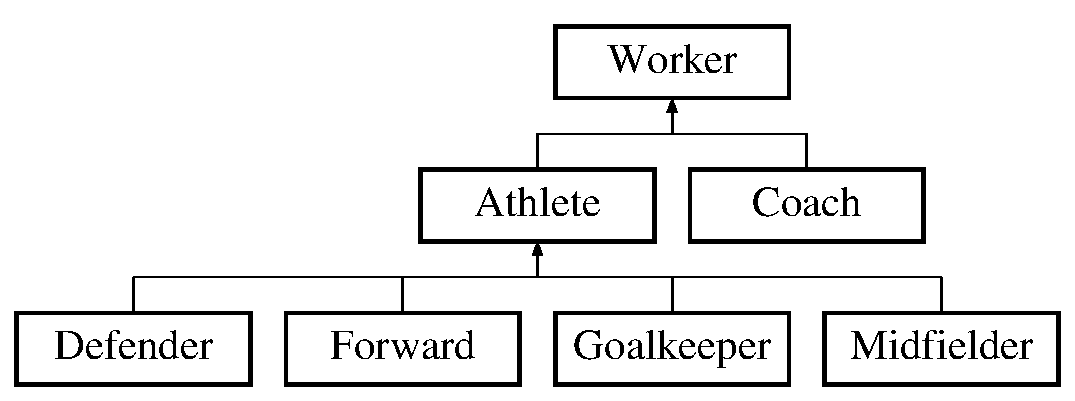
\includegraphics[height=3.000000cm]{class_worker}
\end{center}
\end{figure}
\subsection*{Public Member Functions}
\begin{DoxyCompactItemize}
\item 
\hyperlink{class_worker_a29731c51f83b66fad738b7c66383b62b}{Worker} (string \hyperlink{class_worker_a66cf57341253a31e418cf8abad59ffb1}{name}, \hyperlink{class_date}{Date} \hyperlink{class_worker_a3c1845f40a084b471750a787a87614dd}{birthdate}, unsigned int \hyperlink{class_worker_adfafba55f967994f4595bd914bbba127}{civil\+ID}, unsigned int \hyperlink{class_worker_afc39287cd510977cfe7697ed2c86b2ca}{id}=0)
\begin{DoxyCompactList}\small\item\em \hyperlink{class_worker}{Worker} constructor. \end{DoxyCompactList}\item 
\hyperlink{class_worker_a3754817df06ffe220f7f0d903c78ccac}{Worker} ()
\begin{DoxyCompactList}\small\item\em \hyperlink{class_worker}{Worker} empty constructor. \end{DoxyCompactList}\item 
virtual unsigned int \hyperlink{class_worker_a8b3e221c4a1ebd12ade03ee9b9c86182}{get\+ID} () const =0
\begin{DoxyCompactList}\small\item\em Abstract method -\/ get the worker id. \end{DoxyCompactList}\item 
virtual bool \hyperlink{class_worker_a0a2eb7505b3a734184be3dfdf3316cc3}{is\+Athlete} () const =0
\item 
bool \hyperlink{class_worker_ab2f8a86824ea129ea4d39b6ed7cfe847}{operator==} (\hyperlink{class_worker}{Worker} $\ast$worker) const
\item 
void \hyperlink{class_worker_a7d66047c0683a9a43f89254d0450cd47}{set\+Status} (bool new\+Status)
\item 
void \hyperlink{class_worker_a213180d9f1e4822113f654f7f4ed147c}{set\+Id} (unsigned int new\+Id)
\item 
void \hyperlink{class_worker_ace180f14f1a72e3e018c5ce06c1f3bb3}{set\+Civil\+Id} (unsigned int new\+Civil\+Id)
\item 
virtual void \hyperlink{class_worker_a7d06c15a1d9872d629988aa054996627}{update\+E\+CG} (bool resultado, \hyperlink{class_date}{Date} expiration\+Date=\hyperlink{class_date}{Date}(\hyperlink{class_date}{Date}().get\+Day(), \hyperlink{class_date}{Date}().get\+Month(), \hyperlink{class_date}{Date}().get\+Year()+1))
\begin{DoxyCompactList}\small\item\em Updates the ecg. \end{DoxyCompactList}\item 
void \hyperlink{class_worker_a9113351bf9395094fa0e1d1cfa426881}{set\+Name} (string new\+Name)
\begin{DoxyCompactList}\small\item\em Sets a name. \end{DoxyCompactList}\item 
virtual void \hyperlink{class_worker_ac48a8315ccdeb2913cd98ea223660f72}{set\+Birth\+Date} (\hyperlink{class_date}{Date} new\+Birthdate)
\begin{DoxyCompactList}\small\item\em Sets birth date. \end{DoxyCompactList}\item 
virtual void \hyperlink{class_worker_a64124dca31baa9b110779c7698c15a57}{set\+Height} (unsigned int new\+Height)
\begin{DoxyCompactList}\small\item\em Sets a height. \end{DoxyCompactList}\item 
virtual void \hyperlink{class_worker_ae84b05468a6fdbadad9163bfc18e0569}{set\+Coach\+Type} (\hyperlink{_utils_8hpp_ad6bce769911d709b802464c1ec12e7ad}{Coach\+Type} new\+Type)
\begin{DoxyCompactList}\small\item\em Sets coach type. \end{DoxyCompactList}\item 
\hyperlink{class_worker_aa8e4543ef1e93fd9d884269ba30c5bfe}{$\sim$\+Worker} ()
\item 
unsigned int \hyperlink{class_worker_ae82fdc34f91e5f47dc709d97329a872f}{get\+Age} () const
\begin{DoxyCompactList}\small\item\em Gets the age. \end{DoxyCompactList}\item 
\hyperlink{class_date}{Date} \hyperlink{class_worker_a43fb49c315c8c0a656924e8da285ddf9}{get\+Birthdate} () const
\begin{DoxyCompactList}\small\item\em Gets the birthdate. \end{DoxyCompactList}\item 
virtual \hyperlink{class_info}{Info} $\ast$ \hyperlink{class_worker_a95a4f7c750644937859b8e14515a480e}{get\+Info} () const
\begin{DoxyCompactList}\small\item\em Gets the information. \end{DoxyCompactList}\item 
virtual void \hyperlink{class_worker_ad54db262f7473cc729c371dd54e292eb}{add\+Info} (\hyperlink{class_info}{Info} $\ast$more\+Info)
\begin{DoxyCompactList}\small\item\em Adds an information. \end{DoxyCompactList}\item 
virtual string \hyperlink{class_worker_ac77905603b86c58cb0a87d6389dca744}{generate\+Info} () const
\begin{DoxyCompactList}\small\item\em Generates an information. \end{DoxyCompactList}\item 
string \hyperlink{class_worker_aaaa5808dae61a91b5344224b0ec4d0aa}{get\+Name} () const
\item 
virtual unsigned int \hyperlink{class_worker_a5fd37dea8c5e6579c1deecbfc1b22db9}{get\+Position} () const =0
\item 
virtual unsigned int \hyperlink{class_worker_a1c5dcdc1c7dc5e498a44f678e964bbfd}{get\+Height} () const =0
\item 
virtual \hyperlink{class_e_c_g}{E\+CG} $\ast$ \hyperlink{class_worker_a625cb5da072fd244f38f42e15693058a}{get\+E\+CG} () const
\item 
unsigned int \hyperlink{class_worker_a29fed9c10e4e9a8c1bd4cdfa41add2d2}{get\+Civil\+ID} () const
\item 
virtual vector$<$ string $>$ \hyperlink{class_worker_aca1475c72f6e7c6b85114b0bba0da038}{show\+In\+Screen} () const
\item 
bool \hyperlink{class_worker_a59b1b4769ad7cc740b051e53c986b725}{is\+Active} () const
\end{DoxyCompactItemize}
\subsection*{Static Public Member Functions}
\begin{DoxyCompactItemize}
\item 
static unsigned int \hyperlink{class_worker_ab2ad8ec70eb7a478a3525e5114689625}{get\+Last\+Id} ()
\end{DoxyCompactItemize}
\subsection*{Protected Attributes}
\begin{DoxyCompactItemize}
\item 
string \hyperlink{class_worker_a66cf57341253a31e418cf8abad59ffb1}{name}
\item 
\hyperlink{class_date}{Date} \hyperlink{class_worker_a3c1845f40a084b471750a787a87614dd}{birthdate}
\item 
unsigned int \hyperlink{class_worker_afc39287cd510977cfe7697ed2c86b2ca}{id}
\item 
bool \hyperlink{class_worker_a86618aa5fcac9253f9a7ca0dc16a31d4}{status}
\item 
unsigned int \hyperlink{class_worker_adfafba55f967994f4595bd914bbba127}{civil\+ID}
\end{DoxyCompactItemize}
\subsection*{Static Protected Attributes}
\begin{DoxyCompactItemize}
\item 
static unsigned int \hyperlink{class_worker_a5f0df787d74ab0938583c07a09d126bf}{workers\+Counter} = 0
\end{DoxyCompactItemize}
\subsection*{Friends}
\begin{DoxyCompactItemize}
\item 
ostream \& \hyperlink{class_worker_a8d1e3d13654b0c5466ec0560d2ab7c4e}{operator$<$$<$} (ostream \&out, const \hyperlink{class_worker}{Worker} \&worker)
\begin{DoxyCompactList}\small\item\em Stream insertion operator. \end{DoxyCompactList}\end{DoxyCompactItemize}


\subsection{Detailed Description}
\hyperlink{class_worker}{Worker} Class. 

Represents a club worker, can be either a player or a coach 

\subsection{Constructor \& Destructor Documentation}
\hypertarget{class_worker_a29731c51f83b66fad738b7c66383b62b}{}\label{class_worker_a29731c51f83b66fad738b7c66383b62b} 
\index{Worker@{Worker}!Worker@{Worker}}
\index{Worker@{Worker}!Worker@{Worker}}
\subsubsection{\texorpdfstring{Worker()}{Worker()}\hspace{0.1cm}{\footnotesize\ttfamily [1/2]}}
{\footnotesize\ttfamily Worker\+::\+Worker (\begin{DoxyParamCaption}\item[{string}]{name,  }\item[{\hyperlink{class_date}{Date}}]{birthdate,  }\item[{unsigned int}]{civil\+ID,  }\item[{unsigned int}]{id = {\ttfamily 0} }\end{DoxyParamCaption})}



\hyperlink{class_worker}{Worker} constructor. 


\begin{DoxyParams}{Parameters}
{\em name} & the name of the worker. \\
\hline
{\em birthdate} & the worker birthdate. \\
\hline
\end{DoxyParams}
\hypertarget{class_worker_a3754817df06ffe220f7f0d903c78ccac}{}\label{class_worker_a3754817df06ffe220f7f0d903c78ccac} 
\index{Worker@{Worker}!Worker@{Worker}}
\index{Worker@{Worker}!Worker@{Worker}}
\subsubsection{\texorpdfstring{Worker()}{Worker()}\hspace{0.1cm}{\footnotesize\ttfamily [2/2]}}
{\footnotesize\ttfamily Worker\+::\+Worker (\begin{DoxyParamCaption}{ }\end{DoxyParamCaption})}



\hyperlink{class_worker}{Worker} empty constructor. 

\hypertarget{class_worker_aa8e4543ef1e93fd9d884269ba30c5bfe}{}\label{class_worker_aa8e4543ef1e93fd9d884269ba30c5bfe} 
\index{Worker@{Worker}!````~Worker@{$\sim$\+Worker}}
\index{````~Worker@{$\sim$\+Worker}!Worker@{Worker}}
\subsubsection{\texorpdfstring{$\sim$\+Worker()}{~Worker()}}
{\footnotesize\ttfamily Worker\+::$\sim$\+Worker (\begin{DoxyParamCaption}{ }\end{DoxyParamCaption})}



\subsection{Member Function Documentation}
\hypertarget{class_worker_ad54db262f7473cc729c371dd54e292eb}{}\label{class_worker_ad54db262f7473cc729c371dd54e292eb} 
\index{Worker@{Worker}!add\+Info@{add\+Info}}
\index{add\+Info@{add\+Info}!Worker@{Worker}}
\subsubsection{\texorpdfstring{add\+Info()}{addInfo()}}
{\footnotesize\ttfamily virtual void Worker\+::add\+Info (\begin{DoxyParamCaption}\item[{\hyperlink{class_info}{Info} $\ast$}]{more\+Info }\end{DoxyParamCaption})\hspace{0.3cm}{\ttfamily [inline]}, {\ttfamily [virtual]}}



Adds an information. 

Luís, 20/11/2016. 


\begin{DoxyParams}{Parameters}
{\em more\+Info} & \mbox{[}in,out\mbox{]} If non-\/null, information describing the more. \\
\hline
\end{DoxyParams}


Reimplemented in \hyperlink{class_coach_a989f8c8ec5ba95849503f79376fc68bb}{Coach}, \hyperlink{class_goalkeeper_a97fc43118c67d500d7d56abc9c0029fe}{Goalkeeper}, \hyperlink{class_defender_abcd887808491719d6e40d92d68862b4e}{Defender}, \hyperlink{class_forward_a18f2db8a8234912d6a27727cb3b04fd9}{Forward}, and \hyperlink{class_midfielder_aca69e728b57110b3f34de94556465c0a}{Midfielder}.

\hypertarget{class_worker_ac77905603b86c58cb0a87d6389dca744}{}\label{class_worker_ac77905603b86c58cb0a87d6389dca744} 
\index{Worker@{Worker}!generate\+Info@{generate\+Info}}
\index{generate\+Info@{generate\+Info}!Worker@{Worker}}
\subsubsection{\texorpdfstring{generate\+Info()}{generateInfo()}}
{\footnotesize\ttfamily virtual string Worker\+::generate\+Info (\begin{DoxyParamCaption}{ }\end{DoxyParamCaption}) const\hspace{0.3cm}{\ttfamily [inline]}, {\ttfamily [virtual]}}



Generates an information. 

Luís, 20/11/2016. 

\begin{DoxyReturn}{Returns}
The information. 
\end{DoxyReturn}


Reimplemented in \hyperlink{class_coach_a95f841d14e6994708a7f230a5d3a8d23}{Coach}, and \hyperlink{class_athlete_a44a5a7f1676c6ad2faca9bf51877a6f8}{Athlete}.

\hypertarget{class_worker_ae82fdc34f91e5f47dc709d97329a872f}{}\label{class_worker_ae82fdc34f91e5f47dc709d97329a872f} 
\index{Worker@{Worker}!get\+Age@{get\+Age}}
\index{get\+Age@{get\+Age}!Worker@{Worker}}
\subsubsection{\texorpdfstring{get\+Age()}{getAge()}}
{\footnotesize\ttfamily unsigned int Worker\+::get\+Age (\begin{DoxyParamCaption}{ }\end{DoxyParamCaption}) const}



Gets the age. 

Luís, 20/11/2016. 

\begin{DoxyReturn}{Returns}
The age. 
\end{DoxyReturn}
\hypertarget{class_worker_a43fb49c315c8c0a656924e8da285ddf9}{}\label{class_worker_a43fb49c315c8c0a656924e8da285ddf9} 
\index{Worker@{Worker}!get\+Birthdate@{get\+Birthdate}}
\index{get\+Birthdate@{get\+Birthdate}!Worker@{Worker}}
\subsubsection{\texorpdfstring{get\+Birthdate()}{getBirthdate()}}
{\footnotesize\ttfamily \hyperlink{class_date}{Date} Worker\+::get\+Birthdate (\begin{DoxyParamCaption}{ }\end{DoxyParamCaption}) const}



Gets the birthdate. 

Luís, 20/11/2016. 

\begin{DoxyReturn}{Returns}
The birthdate. 
\end{DoxyReturn}
\hypertarget{class_worker_a29fed9c10e4e9a8c1bd4cdfa41add2d2}{}\label{class_worker_a29fed9c10e4e9a8c1bd4cdfa41add2d2} 
\index{Worker@{Worker}!get\+Civil\+ID@{get\+Civil\+ID}}
\index{get\+Civil\+ID@{get\+Civil\+ID}!Worker@{Worker}}
\subsubsection{\texorpdfstring{get\+Civil\+I\+D()}{getCivilID()}}
{\footnotesize\ttfamily unsigned int Worker\+::get\+Civil\+ID (\begin{DoxyParamCaption}{ }\end{DoxyParamCaption}) const}

\hypertarget{class_worker_a625cb5da072fd244f38f42e15693058a}{}\label{class_worker_a625cb5da072fd244f38f42e15693058a} 
\index{Worker@{Worker}!get\+E\+CG@{get\+E\+CG}}
\index{get\+E\+CG@{get\+E\+CG}!Worker@{Worker}}
\subsubsection{\texorpdfstring{get\+E\+C\+G()}{getECG()}}
{\footnotesize\ttfamily \hyperlink{class_e_c_g}{E\+CG} $\ast$ Worker\+::get\+E\+CG (\begin{DoxyParamCaption}{ }\end{DoxyParamCaption}) const\hspace{0.3cm}{\ttfamily [virtual]}}

This is an abstract method to get the athlete\textquotesingle{}s \hyperlink{class_e_c_g}{E\+CG} 

Reimplemented in \hyperlink{class_athlete_a9655c13ed4126435df2e57e64884deab}{Athlete}.

\hypertarget{class_worker_a1c5dcdc1c7dc5e498a44f678e964bbfd}{}\label{class_worker_a1c5dcdc1c7dc5e498a44f678e964bbfd} 
\index{Worker@{Worker}!get\+Height@{get\+Height}}
\index{get\+Height@{get\+Height}!Worker@{Worker}}
\subsubsection{\texorpdfstring{get\+Height()}{getHeight()}}
{\footnotesize\ttfamily virtual unsigned int Worker\+::get\+Height (\begin{DoxyParamCaption}{ }\end{DoxyParamCaption}) const\hspace{0.3cm}{\ttfamily [pure virtual]}}

This is an abstract method to get the athlete height 

Implemented in \hyperlink{class_coach_af899da3e98bc326b9abdf3ef46cf5279}{Coach}, and \hyperlink{class_athlete_a54a75ed3943dc6b5e229997be8422466}{Athlete}.

\hypertarget{class_worker_a8b3e221c4a1ebd12ade03ee9b9c86182}{}\label{class_worker_a8b3e221c4a1ebd12ade03ee9b9c86182} 
\index{Worker@{Worker}!get\+ID@{get\+ID}}
\index{get\+ID@{get\+ID}!Worker@{Worker}}
\subsubsection{\texorpdfstring{get\+I\+D()}{getID()}}
{\footnotesize\ttfamily unsigned int Worker\+::get\+ID (\begin{DoxyParamCaption}{ }\end{DoxyParamCaption}) const\hspace{0.3cm}{\ttfamily [pure virtual]}}



Abstract method -\/ get the worker id. 

This is an abstract method to make this class abstract 

Implemented in \hyperlink{class_goalkeeper_a61cff0476146d2fc063d5ed7be82a123}{Goalkeeper}, \hyperlink{class_defender_ad2aadb1cb382bf08522bd858ecc69667}{Defender}, \hyperlink{class_coach_a408361901fdbc11fd990b5fa26a94803}{Coach}, \hyperlink{class_forward_aacec6cafa4f965940286bd81e91e1eed}{Forward}, and \hyperlink{class_midfielder_ac55e51de4a6544c30ef2471b6c160d2b}{Midfielder}.

\hypertarget{class_worker_a95a4f7c750644937859b8e14515a480e}{}\label{class_worker_a95a4f7c750644937859b8e14515a480e} 
\index{Worker@{Worker}!get\+Info@{get\+Info}}
\index{get\+Info@{get\+Info}!Worker@{Worker}}
\subsubsection{\texorpdfstring{get\+Info()}{getInfo()}}
{\footnotesize\ttfamily virtual \hyperlink{class_info}{Info}$\ast$ Worker\+::get\+Info (\begin{DoxyParamCaption}{ }\end{DoxyParamCaption}) const\hspace{0.3cm}{\ttfamily [inline]}, {\ttfamily [virtual]}}



Gets the information. 

Luís, 20/11/2016. 

\begin{DoxyReturn}{Returns}
Null if it fails, else the information. 
\end{DoxyReturn}


Reimplemented in \hyperlink{class_coach_a527d675556892403695d70c438d76151}{Coach}, \hyperlink{class_goalkeeper_a8636c061d81440070cf554d5a3923acb}{Goalkeeper}, \hyperlink{class_defender_a54de21eac6353f8847ac109b8a08fcab}{Defender}, \hyperlink{class_forward_a5d8e8085c9a8c95a3296afc40fca81e5}{Forward}, and \hyperlink{class_midfielder_a18c2c163951dd942685950ac562f3b24}{Midfielder}.

\hypertarget{class_worker_ab2ad8ec70eb7a478a3525e5114689625}{}\label{class_worker_ab2ad8ec70eb7a478a3525e5114689625} 
\index{Worker@{Worker}!get\+Last\+Id@{get\+Last\+Id}}
\index{get\+Last\+Id@{get\+Last\+Id}!Worker@{Worker}}
\subsubsection{\texorpdfstring{get\+Last\+Id()}{getLastId()}}
{\footnotesize\ttfamily unsigned int Worker\+::get\+Last\+Id (\begin{DoxyParamCaption}{ }\end{DoxyParamCaption})\hspace{0.3cm}{\ttfamily [static]}}

This is a static method to get the last Id created \hypertarget{class_worker_aaaa5808dae61a91b5344224b0ec4d0aa}{}\label{class_worker_aaaa5808dae61a91b5344224b0ec4d0aa} 
\index{Worker@{Worker}!get\+Name@{get\+Name}}
\index{get\+Name@{get\+Name}!Worker@{Worker}}
\subsubsection{\texorpdfstring{get\+Name()}{getName()}}
{\footnotesize\ttfamily string Worker\+::get\+Name (\begin{DoxyParamCaption}{ }\end{DoxyParamCaption}) const}

\hypertarget{class_worker_a5fd37dea8c5e6579c1deecbfc1b22db9}{}\label{class_worker_a5fd37dea8c5e6579c1deecbfc1b22db9} 
\index{Worker@{Worker}!get\+Position@{get\+Position}}
\index{get\+Position@{get\+Position}!Worker@{Worker}}
\subsubsection{\texorpdfstring{get\+Position()}{getPosition()}}
{\footnotesize\ttfamily virtual unsigned int Worker\+::get\+Position (\begin{DoxyParamCaption}{ }\end{DoxyParamCaption}) const\hspace{0.3cm}{\ttfamily [pure virtual]}}

This is an abstract method to get the athlete or coach position 

Implemented in \hyperlink{class_coach_aa248ee0fec4a5dfdddb8c235ad4ae4a8}{Coach}, and \hyperlink{class_athlete_a18ca289d50900c3825f21d36f2bf8d75}{Athlete}.

\hypertarget{class_worker_a59b1b4769ad7cc740b051e53c986b725}{}\label{class_worker_a59b1b4769ad7cc740b051e53c986b725} 
\index{Worker@{Worker}!is\+Active@{is\+Active}}
\index{is\+Active@{is\+Active}!Worker@{Worker}}
\subsubsection{\texorpdfstring{is\+Active()}{isActive()}}
{\footnotesize\ttfamily bool Worker\+::is\+Active (\begin{DoxyParamCaption}{ }\end{DoxyParamCaption}) const}

\hypertarget{class_worker_a0a2eb7505b3a734184be3dfdf3316cc3}{}\label{class_worker_a0a2eb7505b3a734184be3dfdf3316cc3} 
\index{Worker@{Worker}!is\+Athlete@{is\+Athlete}}
\index{is\+Athlete@{is\+Athlete}!Worker@{Worker}}
\subsubsection{\texorpdfstring{is\+Athlete()}{isAthlete()}}
{\footnotesize\ttfamily virtual bool Worker\+::is\+Athlete (\begin{DoxyParamCaption}{ }\end{DoxyParamCaption}) const\hspace{0.3cm}{\ttfamily [pure virtual]}}

This is an abstract method to check if the object is an \hyperlink{class_athlete}{Athlete} 

Implemented in \hyperlink{class_athlete_a5a6f1744e0944cbabbe333964d6357f4}{Athlete}, and \hyperlink{class_coach_a6329a96f3fea5b02b46b4e6caf519359}{Coach}.

\hypertarget{class_worker_ab2f8a86824ea129ea4d39b6ed7cfe847}{}\label{class_worker_ab2f8a86824ea129ea4d39b6ed7cfe847} 
\index{Worker@{Worker}!operator==@{operator==}}
\index{operator==@{operator==}!Worker@{Worker}}
\subsubsection{\texorpdfstring{operator==()}{operator==()}}
{\footnotesize\ttfamily bool Worker\+::operator== (\begin{DoxyParamCaption}\item[{\hyperlink{class_worker}{Worker} $\ast$}]{worker }\end{DoxyParamCaption}) const}

This is the == operator that returns true if the id\textquotesingle{}s are equal \hypertarget{class_worker_ac48a8315ccdeb2913cd98ea223660f72}{}\label{class_worker_ac48a8315ccdeb2913cd98ea223660f72} 
\index{Worker@{Worker}!set\+Birth\+Date@{set\+Birth\+Date}}
\index{set\+Birth\+Date@{set\+Birth\+Date}!Worker@{Worker}}
\subsubsection{\texorpdfstring{set\+Birth\+Date()}{setBirthDate()}}
{\footnotesize\ttfamily virtual void Worker\+::set\+Birth\+Date (\begin{DoxyParamCaption}\item[{\hyperlink{class_date}{Date}}]{new\+Birthdate }\end{DoxyParamCaption})\hspace{0.3cm}{\ttfamily [inline]}, {\ttfamily [virtual]}}



Sets birth date. 

Luís, 20/11/2016. 


\begin{DoxyParams}{Parameters}
{\em new\+Birthdate} & The new birthdate. \\
\hline
\end{DoxyParams}


Reimplemented in \hyperlink{class_athlete_a73fdec76546be945f02cc2b6d90b99ca}{Athlete}, and \hyperlink{class_coach_aef508cef2680594ef837407790d00db6}{Coach}.

\hypertarget{class_worker_ace180f14f1a72e3e018c5ce06c1f3bb3}{}\label{class_worker_ace180f14f1a72e3e018c5ce06c1f3bb3} 
\index{Worker@{Worker}!set\+Civil\+Id@{set\+Civil\+Id}}
\index{set\+Civil\+Id@{set\+Civil\+Id}!Worker@{Worker}}
\subsubsection{\texorpdfstring{set\+Civil\+Id()}{setCivilId()}}
{\footnotesize\ttfamily void Worker\+::set\+Civil\+Id (\begin{DoxyParamCaption}\item[{unsigned int}]{new\+Civil\+Id }\end{DoxyParamCaption})}

This is the set Civil ID function that actualize the civil ID atribute \hypertarget{class_worker_ae84b05468a6fdbadad9163bfc18e0569}{}\label{class_worker_ae84b05468a6fdbadad9163bfc18e0569} 
\index{Worker@{Worker}!set\+Coach\+Type@{set\+Coach\+Type}}
\index{set\+Coach\+Type@{set\+Coach\+Type}!Worker@{Worker}}
\subsubsection{\texorpdfstring{set\+Coach\+Type()}{setCoachType()}}
{\footnotesize\ttfamily virtual void Worker\+::set\+Coach\+Type (\begin{DoxyParamCaption}\item[{\hyperlink{_utils_8hpp_ad6bce769911d709b802464c1ec12e7ad}{Coach\+Type}}]{new\+Type }\end{DoxyParamCaption})\hspace{0.3cm}{\ttfamily [inline]}, {\ttfamily [virtual]}}



Sets coach type. 

Luís, 20/11/2016. 


\begin{DoxyParams}{Parameters}
{\em new\+Type} & Type of the new. \\
\hline
\end{DoxyParams}


Reimplemented in \hyperlink{class_coach_a72de329d96f180eca4108c7103946ee3}{Coach}.

\hypertarget{class_worker_a64124dca31baa9b110779c7698c15a57}{}\label{class_worker_a64124dca31baa9b110779c7698c15a57} 
\index{Worker@{Worker}!set\+Height@{set\+Height}}
\index{set\+Height@{set\+Height}!Worker@{Worker}}
\subsubsection{\texorpdfstring{set\+Height()}{setHeight()}}
{\footnotesize\ttfamily virtual void Worker\+::set\+Height (\begin{DoxyParamCaption}\item[{unsigned int}]{new\+Height }\end{DoxyParamCaption})\hspace{0.3cm}{\ttfamily [inline]}, {\ttfamily [virtual]}}



Sets a height. 

Luís, 20/11/2016. 


\begin{DoxyParams}{Parameters}
{\em new\+Height} & Height of the new. \\
\hline
\end{DoxyParams}


Reimplemented in \hyperlink{class_athlete_ab96f3138f984bb830aa69f1502961dc8}{Athlete}.

\hypertarget{class_worker_a213180d9f1e4822113f654f7f4ed147c}{}\label{class_worker_a213180d9f1e4822113f654f7f4ed147c} 
\index{Worker@{Worker}!set\+Id@{set\+Id}}
\index{set\+Id@{set\+Id}!Worker@{Worker}}
\subsubsection{\texorpdfstring{set\+Id()}{setId()}}
{\footnotesize\ttfamily void Worker\+::set\+Id (\begin{DoxyParamCaption}\item[{unsigned int}]{new\+Id }\end{DoxyParamCaption})}

This is the set ID function that actualize the ID atribute \hypertarget{class_worker_a9113351bf9395094fa0e1d1cfa426881}{}\label{class_worker_a9113351bf9395094fa0e1d1cfa426881} 
\index{Worker@{Worker}!set\+Name@{set\+Name}}
\index{set\+Name@{set\+Name}!Worker@{Worker}}
\subsubsection{\texorpdfstring{set\+Name()}{setName()}}
{\footnotesize\ttfamily void Worker\+::set\+Name (\begin{DoxyParamCaption}\item[{string}]{new\+Name }\end{DoxyParamCaption})}



Sets a name. 

Luís, 20/11/2016. 


\begin{DoxyParams}{Parameters}
{\em new\+Name} & Name of the new. \\
\hline
\end{DoxyParams}
\hypertarget{class_worker_a7d66047c0683a9a43f89254d0450cd47}{}\label{class_worker_a7d66047c0683a9a43f89254d0450cd47} 
\index{Worker@{Worker}!set\+Status@{set\+Status}}
\index{set\+Status@{set\+Status}!Worker@{Worker}}
\subsubsection{\texorpdfstring{set\+Status()}{setStatus()}}
{\footnotesize\ttfamily void Worker\+::set\+Status (\begin{DoxyParamCaption}\item[{bool}]{new\+Status }\end{DoxyParamCaption})}

This is the set status function that actualize the status atribute \hypertarget{class_worker_aca1475c72f6e7c6b85114b0bba0da038}{}\label{class_worker_aca1475c72f6e7c6b85114b0bba0da038} 
\index{Worker@{Worker}!show\+In\+Screen@{show\+In\+Screen}}
\index{show\+In\+Screen@{show\+In\+Screen}!Worker@{Worker}}
\subsubsection{\texorpdfstring{show\+In\+Screen()}{showInScreen()}}
{\footnotesize\ttfamily vector$<$ string $>$ Worker\+::show\+In\+Screen (\begin{DoxyParamCaption}{ }\end{DoxyParamCaption}) const\hspace{0.3cm}{\ttfamily [virtual]}}



Reimplemented in \hyperlink{class_coach_a954ee94a35267f5992d1a84d25c15c7f}{Coach}, and \hyperlink{class_athlete_a4c7813bb2b52b7095cb7e85aef2e54d5}{Athlete}.

\hypertarget{class_worker_a7d06c15a1d9872d629988aa054996627}{}\label{class_worker_a7d06c15a1d9872d629988aa054996627} 
\index{Worker@{Worker}!update\+E\+CG@{update\+E\+CG}}
\index{update\+E\+CG@{update\+E\+CG}!Worker@{Worker}}
\subsubsection{\texorpdfstring{update\+E\+C\+G()}{updateECG()}}
{\footnotesize\ttfamily void Worker\+::update\+E\+CG (\begin{DoxyParamCaption}\item[{bool}]{resultado,  }\item[{\hyperlink{class_date}{Date}}]{expiration\+Date = {\ttfamily \hyperlink{class_date}{Date}(\hyperlink{class_date}{Date}().getDay(),~\hyperlink{class_date}{Date}().getMonth(),\hyperlink{class_date}{Date}().getYear()+1)} }\end{DoxyParamCaption})\hspace{0.3cm}{\ttfamily [virtual]}}



Updates the ecg. 

Luís, 20/11/2016. 


\begin{DoxyParams}{Parameters}
{\em resultado} & True to resultado. \\
\hline
{\em expiration\+Date} & (Optional) The expiration date. \\
\hline
\end{DoxyParams}


Reimplemented in \hyperlink{class_athlete_a7eda9551e23db1e742a33e9ac61bd42d}{Athlete}.



\subsection{Friends And Related Function Documentation}
\hypertarget{class_worker_a8d1e3d13654b0c5466ec0560d2ab7c4e}{}\label{class_worker_a8d1e3d13654b0c5466ec0560d2ab7c4e} 
\index{Worker@{Worker}!operator$<$$<$@{operator$<$$<$}}
\index{operator$<$$<$@{operator$<$$<$}!Worker@{Worker}}
\subsubsection{\texorpdfstring{operator$<$$<$}{operator<<}}
{\footnotesize\ttfamily ostream\& operator$<$$<$ (\begin{DoxyParamCaption}\item[{ostream \&}]{out,  }\item[{const \hyperlink{class_worker}{Worker} \&}]{worker }\end{DoxyParamCaption})\hspace{0.3cm}{\ttfamily [friend]}}



Stream insertion operator. 

Luís, 20/11/2016. 


\begin{DoxyParams}{Parameters}
{\em out} & \mbox{[}in,out\mbox{]} The out. \\
\hline
{\em worker} & The worker. \\
\hline
\end{DoxyParams}


\begin{DoxyReturn}{Returns}
The shifted result. 
\end{DoxyReturn}


\subsection{Member Data Documentation}
\hypertarget{class_worker_a3c1845f40a084b471750a787a87614dd}{}\label{class_worker_a3c1845f40a084b471750a787a87614dd} 
\index{Worker@{Worker}!birthdate@{birthdate}}
\index{birthdate@{birthdate}!Worker@{Worker}}
\subsubsection{\texorpdfstring{birthdate}{birthdate}}
{\footnotesize\ttfamily \hyperlink{class_date}{Date} Worker\+::birthdate\hspace{0.3cm}{\ttfamily [protected]}}

\hyperlink{class_worker}{Worker} birthdate used to calculate age \hypertarget{class_worker_adfafba55f967994f4595bd914bbba127}{}\label{class_worker_adfafba55f967994f4595bd914bbba127} 
\index{Worker@{Worker}!civil\+ID@{civil\+ID}}
\index{civil\+ID@{civil\+ID}!Worker@{Worker}}
\subsubsection{\texorpdfstring{civil\+ID}{civilID}}
{\footnotesize\ttfamily unsigned int Worker\+::civil\+ID\hspace{0.3cm}{\ttfamily [protected]}}

\hyperlink{class_worker}{Worker} Civil ID \hypertarget{class_worker_afc39287cd510977cfe7697ed2c86b2ca}{}\label{class_worker_afc39287cd510977cfe7697ed2c86b2ca} 
\index{Worker@{Worker}!id@{id}}
\index{id@{id}!Worker@{Worker}}
\subsubsection{\texorpdfstring{id}{id}}
{\footnotesize\ttfamily unsigned int Worker\+::id\hspace{0.3cm}{\ttfamily [protected]}}

\hyperlink{class_worker}{Worker} unique id for each club worker \hypertarget{class_worker_a66cf57341253a31e418cf8abad59ffb1}{}\label{class_worker_a66cf57341253a31e418cf8abad59ffb1} 
\index{Worker@{Worker}!name@{name}}
\index{name@{name}!Worker@{Worker}}
\subsubsection{\texorpdfstring{name}{name}}
{\footnotesize\ttfamily string Worker\+::name\hspace{0.3cm}{\ttfamily [protected]}}

\hyperlink{class_worker}{Worker} name \hypertarget{class_worker_a86618aa5fcac9253f9a7ca0dc16a31d4}{}\label{class_worker_a86618aa5fcac9253f9a7ca0dc16a31d4} 
\index{Worker@{Worker}!status@{status}}
\index{status@{status}!Worker@{Worker}}
\subsubsection{\texorpdfstring{status}{status}}
{\footnotesize\ttfamily bool Worker\+::status\hspace{0.3cm}{\ttfamily [protected]}}

\hyperlink{class_worker}{Worker} current status \hypertarget{class_worker_a5f0df787d74ab0938583c07a09d126bf}{}\label{class_worker_a5f0df787d74ab0938583c07a09d126bf} 
\index{Worker@{Worker}!workers\+Counter@{workers\+Counter}}
\index{workers\+Counter@{workers\+Counter}!Worker@{Worker}}
\subsubsection{\texorpdfstring{workers\+Counter}{workersCounter}}
{\footnotesize\ttfamily unsigned int Worker\+::workers\+Counter = 0\hspace{0.3cm}{\ttfamily [static]}, {\ttfamily [protected]}}

\hyperlink{class_worker}{Worker} counter to keep track and generate the ids 

The documentation for this class was generated from the following files\+:\begin{DoxyCompactItemize}
\item 
\hyperlink{_worker_8hpp}{Worker.\+hpp}\item 
\hyperlink{_worker_8cpp}{Worker.\+cpp}\end{DoxyCompactItemize}

\chapter{File Documentation}
\hypertarget{_athlete_8cpp}{}\section{Athlete.\+cpp File Reference}
\label{_athlete_8cpp}\index{Athlete.\+cpp@{Athlete.\+cpp}}
{\ttfamily \#include \char`\"{}Athlete.\+hpp\char`\"{}}\newline

\hypertarget{_athlete_8hpp}{}\section{Athlete.\+hpp File Reference}
\label{_athlete_8hpp}\index{Athlete.\+hpp@{Athlete.\+hpp}}
{\ttfamily \#include \char`\"{}Coach.\+hpp\char`\"{}}\newline
\subsection*{Classes}
\begin{DoxyCompactItemize}
\item 
class \hyperlink{class_athlete}{Athlete}
\begin{DoxyCompactList}\small\item\em An athlete. \end{DoxyCompactList}\end{DoxyCompactItemize}
\subsection*{Macros}
\begin{DoxyCompactItemize}
\item 
\#define \hyperlink{_athlete_8hpp_a5750cdf72871669540c953af9523ae99}{Athlete\+\_\+hpp}
\end{DoxyCompactItemize}


\subsection{Macro Definition Documentation}
\hypertarget{_athlete_8hpp_a5750cdf72871669540c953af9523ae99}{}\label{_athlete_8hpp_a5750cdf72871669540c953af9523ae99} 
\index{Athlete.\+hpp@{Athlete.\+hpp}!Athlete\+\_\+hpp@{Athlete\+\_\+hpp}}
\index{Athlete\+\_\+hpp@{Athlete\+\_\+hpp}!Athlete.\+hpp@{Athlete.\+hpp}}
\subsubsection{\texorpdfstring{Athlete\+\_\+hpp}{Athlete\_hpp}}
{\footnotesize\ttfamily \#define Athlete\+\_\+hpp}


\hypertarget{_b_s_t_8h}{}\section{B\+S\+T.\+h File Reference}
\label{_b_s_t_8h}\index{B\+S\+T.\+h@{B\+S\+T.\+h}}
{\ttfamily \#include $<$iostream$>$}\newline
{\ttfamily \#include $<$stack$>$}\newline
{\ttfamily \#include $<$queue$>$}\newline
\subsection*{Classes}
\begin{DoxyCompactItemize}
\item 
class \hyperlink{class_b_t_itr_in}{B\+T\+Itr\+In$<$ T $>$}
\begin{DoxyCompactList}\small\item\em An in binary tree iterator. \end{DoxyCompactList}\item 
class \hyperlink{class_b_t_itr_pre}{B\+T\+Itr\+Pre$<$ T $>$}
\begin{DoxyCompactList}\small\item\em A pre binary tree iterator. \end{DoxyCompactList}\item 
class \hyperlink{class_b_t_itr_post}{B\+T\+Itr\+Post$<$ T $>$}
\begin{DoxyCompactList}\small\item\em A post binary tree iterator. \end{DoxyCompactList}\item 
class \hyperlink{class_b_t_itr_level}{B\+T\+Itr\+Level$<$ T $>$}
\begin{DoxyCompactList}\small\item\em A level binary tree iterator. \end{DoxyCompactList}\item 
class \hyperlink{class_binary_tree}{Binary\+Tree$<$ T $>$}
\begin{DoxyCompactList}\small\item\em A binary tree. \end{DoxyCompactList}\item 
class \hyperlink{class_underflow}{Underflow}
\begin{DoxyCompactList}\small\item\em An underflow. \end{DoxyCompactList}\item 
class \hyperlink{class_b_t_node}{B\+T\+Node$<$ T $>$}
\begin{DoxyCompactList}\small\item\em A binary tree node. \end{DoxyCompactList}\item 
class \hyperlink{class_binary_tree}{Binary\+Tree$<$ T $>$}
\begin{DoxyCompactList}\small\item\em A binary tree. \end{DoxyCompactList}\item 
class \hyperlink{class_b_t_itr_post}{B\+T\+Itr\+Post$<$ T $>$}
\begin{DoxyCompactList}\small\item\em A post binary tree iterator. \end{DoxyCompactList}\item 
class \hyperlink{class_b_t_itr_pre}{B\+T\+Itr\+Pre$<$ T $>$}
\begin{DoxyCompactList}\small\item\em A pre binary tree iterator. \end{DoxyCompactList}\item 
class \hyperlink{class_b_t_itr_in}{B\+T\+Itr\+In$<$ T $>$}
\begin{DoxyCompactList}\small\item\em An in binary tree iterator. \end{DoxyCompactList}\item 
class \hyperlink{class_b_t_itr_level}{B\+T\+Itr\+Level$<$ T $>$}
\begin{DoxyCompactList}\small\item\em A level binary tree iterator. \end{DoxyCompactList}\end{DoxyCompactItemize}
\subsection*{Macros}
\begin{DoxyCompactItemize}
\item 
\#define \hyperlink{_b_s_t_8h_ac02da2e3786b0be4a93b7620c46e6e22}{\+\_\+\+B\+I\+N\+A\+R\+Y\+\_\+\+T\+R\+E\+E\+\_\+H}
\end{DoxyCompactItemize}
\subsection*{Functions}
\begin{DoxyCompactItemize}
\item 
{\footnotesize template$<$class T $>$ }\\ostream \& \hyperlink{_b_s_t_8h_a54bcac3e6a2991f97116c8191e2df8eb}{operator$<$$<$} (ostream \&out, const \hyperlink{class_binary_tree}{Binary\+Tree}$<$ T $>$ \&t)
\begin{DoxyCompactList}\small\item\em Cast that converts the given ostream into a binary tree; \end{DoxyCompactList}\end{DoxyCompactItemize}


\subsection{Macro Definition Documentation}
\hypertarget{_b_s_t_8h_ac02da2e3786b0be4a93b7620c46e6e22}{}\label{_b_s_t_8h_ac02da2e3786b0be4a93b7620c46e6e22} 
\index{B\+S\+T.\+h@{B\+S\+T.\+h}!\+\_\+\+B\+I\+N\+A\+R\+Y\+\_\+\+T\+R\+E\+E\+\_\+H@{\+\_\+\+B\+I\+N\+A\+R\+Y\+\_\+\+T\+R\+E\+E\+\_\+H}}
\index{\+\_\+\+B\+I\+N\+A\+R\+Y\+\_\+\+T\+R\+E\+E\+\_\+H@{\+\_\+\+B\+I\+N\+A\+R\+Y\+\_\+\+T\+R\+E\+E\+\_\+H}!B\+S\+T.\+h@{B\+S\+T.\+h}}
\subsubsection{\texorpdfstring{\+\_\+\+B\+I\+N\+A\+R\+Y\+\_\+\+T\+R\+E\+E\+\_\+H}{\_BINARY\_TREE\_H}}
{\footnotesize\ttfamily \#define \+\_\+\+B\+I\+N\+A\+R\+Y\+\_\+\+T\+R\+E\+E\+\_\+H}



\subsection{Function Documentation}
\hypertarget{_b_s_t_8h_a54bcac3e6a2991f97116c8191e2df8eb}{}\label{_b_s_t_8h_a54bcac3e6a2991f97116c8191e2df8eb} 
\index{B\+S\+T.\+h@{B\+S\+T.\+h}!operator$<$$<$@{operator$<$$<$}}
\index{operator$<$$<$@{operator$<$$<$}!B\+S\+T.\+h@{B\+S\+T.\+h}}
\subsubsection{\texorpdfstring{operator$<$$<$()}{operator<<()}}
{\footnotesize\ttfamily template$<$class T $>$ \\
ostream\& operator$<$$<$ (\begin{DoxyParamCaption}\item[{ostream \&}]{out,  }\item[{const \hyperlink{class_binary_tree}{Binary\+Tree}$<$ T $>$ \&}]{t }\end{DoxyParamCaption})}



Cast that converts the given ostream into a binary tree; 

Lu�s, 20/11/2016. 


\begin{DoxyParams}{Parameters}
{\em out} & \mbox{[}in,out\mbox{]} The outfile. \\
\hline
{\em t} & The binary tree to process. \\
\hline
\end{DoxyParams}


\begin{DoxyReturn}{Returns}
The result of the operation. 
\end{DoxyReturn}

\hypertarget{_club_8cpp}{}\section{Club.\+cpp File Reference}
\label{_club_8cpp}\index{Club.\+cpp@{Club.\+cpp}}
{\ttfamily \#include \char`\"{}Club.\+hpp\char`\"{}}\newline
{\ttfamily \#include \char`\"{}Season.\+hpp\char`\"{}}\newline
{\ttfamily \#include \char`\"{}Match.\+hpp\char`\"{}}\newline
{\ttfamily \#include \char`\"{}Level.\+h\char`\"{}}\newline

\hypertarget{_club_8hpp}{}\section{Club.\+hpp File Reference}
\label{_club_8hpp}\index{Club.\+hpp@{Club.\+hpp}}
{\ttfamily \#include \char`\"{}Goalkeeper.\+hpp\char`\"{}}\newline
{\ttfamily \#include \char`\"{}Forward.\+hpp\char`\"{}}\newline
\subsection*{Classes}
\begin{DoxyCompactItemize}
\item 
class \hyperlink{class_club}{Club}
\begin{DoxyCompactList}\small\item\em A club. \end{DoxyCompactList}\end{DoxyCompactItemize}
\subsection*{Functions}
\begin{DoxyCompactItemize}
\item 
bool \hyperlink{_club_8hpp_aba1d31da0cee422234dab65e959d075a}{confirm} (const \hyperlink{class_table}{Table} \&message)
\begin{DoxyCompactList}\small\item\em Confirms the given message. \end{DoxyCompactList}\item 
void \hyperlink{_club_8hpp_a048da20072517ef177c79ce2940833d4}{show\+Main\+Menu} (unsigned short int option\+Chosen, string season\+Name)
\begin{DoxyCompactList}\small\item\em Shows the main menu. \end{DoxyCompactList}\end{DoxyCompactItemize}
\subsection*{Variables}
\begin{DoxyCompactItemize}
\item 
const map$<$ string, \hyperlink{_utils_8hpp_ad6bce769911d709b802464c1ec12e7ad}{Coach\+Type} $>$ \hyperlink{_club_8hpp_abcccd5e447418046556559994cfc522d}{coach\+Type\+Map}
\begin{DoxyCompactList}\small\item\em The coach type map. \end{DoxyCompactList}\item 
const map$<$ string, \hyperlink{_utils_8hpp_a226b190c54f09ab6ba8ac83b28e3c4b6}{age\+Level} $>$ \hyperlink{_club_8hpp_afe2a835516f3d8fb7eaa7bc6cd1cf961}{age\+Level\+Map}
\begin{DoxyCompactList}\small\item\em The age level map. \end{DoxyCompactList}\end{DoxyCompactItemize}


\subsection{Function Documentation}
\hypertarget{_club_8hpp_aba1d31da0cee422234dab65e959d075a}{}\label{_club_8hpp_aba1d31da0cee422234dab65e959d075a} 
\index{Club.\+hpp@{Club.\+hpp}!confirm@{confirm}}
\index{confirm@{confirm}!Club.\+hpp@{Club.\+hpp}}
\subsubsection{\texorpdfstring{confirm()}{confirm()}}
{\footnotesize\ttfamily bool confirm (\begin{DoxyParamCaption}\item[{const \hyperlink{class_table}{Table} \&}]{message }\end{DoxyParamCaption})}



Confirms the given message. 

Luís, 20/11/2016. 


\begin{DoxyParams}{Parameters}
{\em message} & The message. \\
\hline
\end{DoxyParams}


\begin{DoxyReturn}{Returns}
True if it succeeds, false if it fails. 
\end{DoxyReturn}
\hypertarget{_club_8hpp_a048da20072517ef177c79ce2940833d4}{}\label{_club_8hpp_a048da20072517ef177c79ce2940833d4} 
\index{Club.\+hpp@{Club.\+hpp}!show\+Main\+Menu@{show\+Main\+Menu}}
\index{show\+Main\+Menu@{show\+Main\+Menu}!Club.\+hpp@{Club.\+hpp}}
\subsubsection{\texorpdfstring{show\+Main\+Menu()}{showMainMenu()}}
{\footnotesize\ttfamily void show\+Main\+Menu (\begin{DoxyParamCaption}\item[{unsigned short int}]{option\+Chosen,  }\item[{string}]{season\+Name }\end{DoxyParamCaption})}



Shows the main menu. 

Luís, 20/11/2016. 


\begin{DoxyParams}{Parameters}
{\em option\+Chosen} & The option chosen. \\
\hline
{\em season\+Name} & Name of the season. \\
\hline
\end{DoxyParams}


\subsection{Variable Documentation}
\hypertarget{_club_8hpp_afe2a835516f3d8fb7eaa7bc6cd1cf961}{}\label{_club_8hpp_afe2a835516f3d8fb7eaa7bc6cd1cf961} 
\index{Club.\+hpp@{Club.\+hpp}!age\+Level\+Map@{age\+Level\+Map}}
\index{age\+Level\+Map@{age\+Level\+Map}!Club.\+hpp@{Club.\+hpp}}
\subsubsection{\texorpdfstring{age\+Level\+Map}{ageLevelMap}}
{\footnotesize\ttfamily const map$<$string, \hyperlink{_utils_8hpp_a226b190c54f09ab6ba8ac83b28e3c4b6}{age\+Level}$>$ age\+Level\+Map}



The age level map. 

\hypertarget{_club_8hpp_abcccd5e447418046556559994cfc522d}{}\label{_club_8hpp_abcccd5e447418046556559994cfc522d} 
\index{Club.\+hpp@{Club.\+hpp}!coach\+Type\+Map@{coach\+Type\+Map}}
\index{coach\+Type\+Map@{coach\+Type\+Map}!Club.\+hpp@{Club.\+hpp}}
\subsubsection{\texorpdfstring{coach\+Type\+Map}{coachTypeMap}}
{\footnotesize\ttfamily const map$<$string, \hyperlink{_utils_8hpp_ad6bce769911d709b802464c1ec12e7ad}{Coach\+Type}$>$ coach\+Type\+Map}



The coach type map. 


\hypertarget{_coach_8cpp}{}\section{Coach.\+cpp File Reference}
\label{_coach_8cpp}\index{Coach.\+cpp@{Coach.\+cpp}}
{\ttfamily \#include \char`\"{}Coach.\+hpp\char`\"{}}\newline

\hypertarget{_coach_8hpp}{}\section{Coach.\+hpp File Reference}
\label{_coach_8hpp}\index{Coach.\+hpp@{Coach.\+hpp}}
{\ttfamily \#include \char`\"{}Worker.\+hpp\char`\"{}}\newline
\subsection*{Classes}
\begin{DoxyCompactItemize}
\item 
class \hyperlink{class_coach}{Coach}
\begin{DoxyCompactList}\small\item\em A coach. \end{DoxyCompactList}\end{DoxyCompactItemize}

\hypertarget{_defender_8cpp}{}\section{Defender.\+cpp File Reference}
\label{_defender_8cpp}\index{Defender.\+cpp@{Defender.\+cpp}}
{\ttfamily \#include \char`\"{}Defender.\+hpp\char`\"{}}\newline

\hypertarget{_defender_8hpp}{}\section{Defender.\+hpp File Reference}
\label{_defender_8hpp}\index{Defender.\+hpp@{Defender.\+hpp}}
{\ttfamily \#include \char`\"{}Midfielder.\+hpp\char`\"{}}\newline
\subsection*{Classes}
\begin{DoxyCompactItemize}
\item 
class \hyperlink{class_defender}{Defender}
\begin{DoxyCompactList}\small\item\em A defender. \end{DoxyCompactList}\end{DoxyCompactItemize}
\subsection*{Macros}
\begin{DoxyCompactItemize}
\item 
\#define \hyperlink{_defender_8hpp_a6c83e9d5e217d209c43d6c1c8dbd3b6d}{Defender\+\_\+hpp}
\end{DoxyCompactItemize}


\subsection{Macro Definition Documentation}
\hypertarget{_defender_8hpp_a6c83e9d5e217d209c43d6c1c8dbd3b6d}{}\label{_defender_8hpp_a6c83e9d5e217d209c43d6c1c8dbd3b6d} 
\index{Defender.\+hpp@{Defender.\+hpp}!Defender\+\_\+hpp@{Defender\+\_\+hpp}}
\index{Defender\+\_\+hpp@{Defender\+\_\+hpp}!Defender.\+hpp@{Defender.\+hpp}}
\subsubsection{\texorpdfstring{Defender\+\_\+hpp}{Defender\_hpp}}
{\footnotesize\ttfamily \#define Defender\+\_\+hpp}


\hypertarget{_e_c_g_8cpp}{}\section{E\+C\+G.\+cpp File Reference}
\label{_e_c_g_8cpp}\index{E\+C\+G.\+cpp@{E\+C\+G.\+cpp}}
{\ttfamily \#include \char`\"{}E\+C\+G.\+hpp\char`\"{}}\newline

\hypertarget{_e_c_g_8hpp}{}\section{E\+C\+G.\+hpp File Reference}
\label{_e_c_g_8hpp}\index{E\+C\+G.\+hpp@{E\+C\+G.\+hpp}}
{\ttfamily \#include \char`\"{}Info\+Athletes.\+hpp\char`\"{}}\newline
\subsection*{Classes}
\begin{DoxyCompactItemize}
\item 
class \hyperlink{class_e_c_g}{E\+CG}
\begin{DoxyCompactList}\small\item\em An ecg. \end{DoxyCompactList}\end{DoxyCompactItemize}
\subsection*{Macros}
\begin{DoxyCompactItemize}
\item 
\#define \hyperlink{_e_c_g_8hpp_aacd257044f98abaf69d28e1464291c15}{E\+C\+G\+\_\+hpp}
\end{DoxyCompactItemize}


\subsection{Macro Definition Documentation}
\hypertarget{_e_c_g_8hpp_aacd257044f98abaf69d28e1464291c15}{}\label{_e_c_g_8hpp_aacd257044f98abaf69d28e1464291c15} 
\index{E\+C\+G.\+hpp@{E\+C\+G.\+hpp}!E\+C\+G\+\_\+hpp@{E\+C\+G\+\_\+hpp}}
\index{E\+C\+G\+\_\+hpp@{E\+C\+G\+\_\+hpp}!E\+C\+G.\+hpp@{E\+C\+G.\+hpp}}
\subsubsection{\texorpdfstring{E\+C\+G\+\_\+hpp}{ECG\_hpp}}
{\footnotesize\ttfamily \#define E\+C\+G\+\_\+hpp}


\hypertarget{_exceptions_8cpp}{}\section{Exceptions.\+cpp File Reference}
\label{_exceptions_8cpp}\index{Exceptions.\+cpp@{Exceptions.\+cpp}}
{\ttfamily \#include \char`\"{}Exceptions.\+hpp\char`\"{}}\newline

\hypertarget{_exceptions_8hpp}{}\section{Exceptions.\+hpp File Reference}
\label{_exceptions_8hpp}\index{Exceptions.\+hpp@{Exceptions.\+hpp}}
{\ttfamily \#include $<$stdio.\+h$>$}\newline
{\ttfamily \#include $<$string$>$}\newline
\subsection*{Classes}
\begin{DoxyCompactItemize}
\item 
class \hyperlink{class_invalid_date}{Invalid\+Date}
\begin{DoxyCompactList}\small\item\em An invalid date. \end{DoxyCompactList}\item 
class \hyperlink{class_invalid_stream}{Invalid\+Stream}
\begin{DoxyCompactList}\small\item\em An invalid stream. \end{DoxyCompactList}\item 
class \hyperlink{class_invalid_input}{Invalid\+Input}
\begin{DoxyCompactList}\small\item\em An invalid input. \end{DoxyCompactList}\end{DoxyCompactItemize}
\subsection*{Enumerations}
\begin{DoxyCompactItemize}
\item 
enum \hyperlink{_exceptions_8hpp_a3c07f150c56e3659483593a47dafc0e3}{Date\+Exception\+Type} \{ \newline
\hyperlink{_exceptions_8hpp_a3c07f150c56e3659483593a47dafc0e3ac8a2781a3a26c629de347bb72e20ea4f}{Invalid\+Day}, 
\hyperlink{_exceptions_8hpp_a3c07f150c56e3659483593a47dafc0e3a54767c7b71c22c93ea05783dec0f8c9c}{Invalid\+Month}, 
\hyperlink{_exceptions_8hpp_a3c07f150c56e3659483593a47dafc0e3ab1afa53fe865da8026fd392e9de6d3e2}{Invalid\+Year}, 
\hyperlink{_exceptions_8hpp_a3c07f150c56e3659483593a47dafc0e3a613fa88fb2700c04545b7ab2f58a3872}{Invalid\+Separators}, 
\newline
\hyperlink{_exceptions_8hpp_a3c07f150c56e3659483593a47dafc0e3a7dc85a46620e365933f9cdcebaf11fe4}{Out\+Of\+Bounds\+Min}, 
\hyperlink{_exceptions_8hpp_a3c07f150c56e3659483593a47dafc0e3a58754c47e13e44449c4e6a8a84f8d227}{Out\+Of\+Bounds\+Max}
 \}\begin{DoxyCompactList}\small\item\em Values that represent date exception types. \end{DoxyCompactList}
\item 
enum \hyperlink{_exceptions_8hpp_a20debbce0a9d256d07eac93067032a39}{Invalid\+Stream\+Type} \{ \hyperlink{_exceptions_8hpp_a20debbce0a9d256d07eac93067032a39aae835b662be01cdc3752f7db84529cca}{write}, 
\hyperlink{_exceptions_8hpp_a20debbce0a9d256d07eac93067032a39aea7c12cb3031ad9e88104ce9859ce1c5}{read}
 \}\begin{DoxyCompactList}\small\item\em Values that represent invalid stream types. \end{DoxyCompactList}
\end{DoxyCompactItemize}


\subsection{Enumeration Type Documentation}
\hypertarget{_exceptions_8hpp_a3c07f150c56e3659483593a47dafc0e3}{}\label{_exceptions_8hpp_a3c07f150c56e3659483593a47dafc0e3} 
\index{Exceptions.\+hpp@{Exceptions.\+hpp}!Date\+Exception\+Type@{Date\+Exception\+Type}}
\index{Date\+Exception\+Type@{Date\+Exception\+Type}!Exceptions.\+hpp@{Exceptions.\+hpp}}
\subsubsection{\texorpdfstring{Date\+Exception\+Type}{DateExceptionType}}
{\footnotesize\ttfamily enum \hyperlink{_exceptions_8hpp_a3c07f150c56e3659483593a47dafc0e3}{Date\+Exception\+Type}}



Values that represent date exception types. 

Luís, 20/11/2016. \begin{DoxyEnumFields}{Enumerator}
\raisebox{\heightof{T}}[0pt][0pt]{\index{Invalid\+Day@{Invalid\+Day}!Exceptions.\+hpp@{Exceptions.\+hpp}}\index{Exceptions.\+hpp@{Exceptions.\+hpp}!Invalid\+Day@{Invalid\+Day}}}\hypertarget{_exceptions_8hpp_a3c07f150c56e3659483593a47dafc0e3ac8a2781a3a26c629de347bb72e20ea4f}{}\label{_exceptions_8hpp_a3c07f150c56e3659483593a47dafc0e3ac8a2781a3a26c629de347bb72e20ea4f} 
Invalid\+Day&\\
\hline

\raisebox{\heightof{T}}[0pt][0pt]{\index{Invalid\+Month@{Invalid\+Month}!Exceptions.\+hpp@{Exceptions.\+hpp}}\index{Exceptions.\+hpp@{Exceptions.\+hpp}!Invalid\+Month@{Invalid\+Month}}}\hypertarget{_exceptions_8hpp_a3c07f150c56e3659483593a47dafc0e3a54767c7b71c22c93ea05783dec0f8c9c}{}\label{_exceptions_8hpp_a3c07f150c56e3659483593a47dafc0e3a54767c7b71c22c93ea05783dec0f8c9c} 
Invalid\+Month&\\
\hline

\raisebox{\heightof{T}}[0pt][0pt]{\index{Invalid\+Year@{Invalid\+Year}!Exceptions.\+hpp@{Exceptions.\+hpp}}\index{Exceptions.\+hpp@{Exceptions.\+hpp}!Invalid\+Year@{Invalid\+Year}}}\hypertarget{_exceptions_8hpp_a3c07f150c56e3659483593a47dafc0e3ab1afa53fe865da8026fd392e9de6d3e2}{}\label{_exceptions_8hpp_a3c07f150c56e3659483593a47dafc0e3ab1afa53fe865da8026fd392e9de6d3e2} 
Invalid\+Year&\\
\hline

\raisebox{\heightof{T}}[0pt][0pt]{\index{Invalid\+Separators@{Invalid\+Separators}!Exceptions.\+hpp@{Exceptions.\+hpp}}\index{Exceptions.\+hpp@{Exceptions.\+hpp}!Invalid\+Separators@{Invalid\+Separators}}}\hypertarget{_exceptions_8hpp_a3c07f150c56e3659483593a47dafc0e3a613fa88fb2700c04545b7ab2f58a3872}{}\label{_exceptions_8hpp_a3c07f150c56e3659483593a47dafc0e3a613fa88fb2700c04545b7ab2f58a3872} 
Invalid\+Separators&\\
\hline

\raisebox{\heightof{T}}[0pt][0pt]{\index{Out\+Of\+Bounds\+Min@{Out\+Of\+Bounds\+Min}!Exceptions.\+hpp@{Exceptions.\+hpp}}\index{Exceptions.\+hpp@{Exceptions.\+hpp}!Out\+Of\+Bounds\+Min@{Out\+Of\+Bounds\+Min}}}\hypertarget{_exceptions_8hpp_a3c07f150c56e3659483593a47dafc0e3a7dc85a46620e365933f9cdcebaf11fe4}{}\label{_exceptions_8hpp_a3c07f150c56e3659483593a47dafc0e3a7dc85a46620e365933f9cdcebaf11fe4} 
Out\+Of\+Bounds\+Min&\\
\hline

\raisebox{\heightof{T}}[0pt][0pt]{\index{Out\+Of\+Bounds\+Max@{Out\+Of\+Bounds\+Max}!Exceptions.\+hpp@{Exceptions.\+hpp}}\index{Exceptions.\+hpp@{Exceptions.\+hpp}!Out\+Of\+Bounds\+Max@{Out\+Of\+Bounds\+Max}}}\hypertarget{_exceptions_8hpp_a3c07f150c56e3659483593a47dafc0e3a58754c47e13e44449c4e6a8a84f8d227}{}\label{_exceptions_8hpp_a3c07f150c56e3659483593a47dafc0e3a58754c47e13e44449c4e6a8a84f8d227} 
Out\+Of\+Bounds\+Max&\\
\hline

\end{DoxyEnumFields}
\hypertarget{_exceptions_8hpp_a20debbce0a9d256d07eac93067032a39}{}\label{_exceptions_8hpp_a20debbce0a9d256d07eac93067032a39} 
\index{Exceptions.\+hpp@{Exceptions.\+hpp}!Invalid\+Stream\+Type@{Invalid\+Stream\+Type}}
\index{Invalid\+Stream\+Type@{Invalid\+Stream\+Type}!Exceptions.\+hpp@{Exceptions.\+hpp}}
\subsubsection{\texorpdfstring{Invalid\+Stream\+Type}{InvalidStreamType}}
{\footnotesize\ttfamily enum \hyperlink{_exceptions_8hpp_a20debbce0a9d256d07eac93067032a39}{Invalid\+Stream\+Type}}



Values that represent invalid stream types. 

Luís, 20/11/2016. \begin{DoxyEnumFields}{Enumerator}
\raisebox{\heightof{T}}[0pt][0pt]{\index{write@{write}!Exceptions.\+hpp@{Exceptions.\+hpp}}\index{Exceptions.\+hpp@{Exceptions.\+hpp}!write@{write}}}\hypertarget{_exceptions_8hpp_a20debbce0a9d256d07eac93067032a39aae835b662be01cdc3752f7db84529cca}{}\label{_exceptions_8hpp_a20debbce0a9d256d07eac93067032a39aae835b662be01cdc3752f7db84529cca} 
write&\\
\hline

\raisebox{\heightof{T}}[0pt][0pt]{\index{read@{read}!Exceptions.\+hpp@{Exceptions.\+hpp}}\index{Exceptions.\+hpp@{Exceptions.\+hpp}!read@{read}}}\hypertarget{_exceptions_8hpp_a20debbce0a9d256d07eac93067032a39aea7c12cb3031ad9e88104ce9859ce1c5}{}\label{_exceptions_8hpp_a20debbce0a9d256d07eac93067032a39aea7c12cb3031ad9e88104ce9859ce1c5} 
read&\\
\hline

\end{DoxyEnumFields}

\hypertarget{_forward_8cpp}{}\section{Forward.\+cpp File Reference}
\label{_forward_8cpp}\index{Forward.\+cpp@{Forward.\+cpp}}
{\ttfamily \#include \char`\"{}Forward.\+hpp\char`\"{}}\newline

\hypertarget{_forward_8hpp}{}\section{Forward.\+hpp File Reference}
\label{_forward_8hpp}\index{Forward.\+hpp@{Forward.\+hpp}}
{\ttfamily \#include \char`\"{}Athlete.\+hpp\char`\"{}}\newline
\subsection*{Classes}
\begin{DoxyCompactItemize}
\item 
class \hyperlink{class_forward}{Forward}
\begin{DoxyCompactList}\small\item\em A forward. \end{DoxyCompactList}\end{DoxyCompactItemize}

\hypertarget{_goalkeeper_8cpp}{}\section{Goalkeeper.\+cpp File Reference}
\label{_goalkeeper_8cpp}\index{Goalkeeper.\+cpp@{Goalkeeper.\+cpp}}
{\ttfamily \#include \char`\"{}Goalkeeper.\+hpp\char`\"{}}\newline

\hypertarget{_goalkeeper_8hpp}{}\section{Goalkeeper.\+hpp File Reference}
\label{_goalkeeper_8hpp}\index{Goalkeeper.\+hpp@{Goalkeeper.\+hpp}}
{\ttfamily \#include \char`\"{}Defender.\+hpp\char`\"{}}\newline
\subsection*{Classes}
\begin{DoxyCompactItemize}
\item 
class \hyperlink{class_goalkeeper}{Goalkeeper}
\end{DoxyCompactItemize}
\subsection*{Macros}
\begin{DoxyCompactItemize}
\item 
\#define \hyperlink{_goalkeeper_8hpp_a06e77e9040a0f51f9444cb01b5a2ede6}{Goalkeeper\+\_\+hpp}
\end{DoxyCompactItemize}


\subsection{Macro Definition Documentation}
\hypertarget{_goalkeeper_8hpp_a06e77e9040a0f51f9444cb01b5a2ede6}{}\label{_goalkeeper_8hpp_a06e77e9040a0f51f9444cb01b5a2ede6} 
\index{Goalkeeper.\+hpp@{Goalkeeper.\+hpp}!Goalkeeper\+\_\+hpp@{Goalkeeper\+\_\+hpp}}
\index{Goalkeeper\+\_\+hpp@{Goalkeeper\+\_\+hpp}!Goalkeeper.\+hpp@{Goalkeeper.\+hpp}}
\subsubsection{\texorpdfstring{Goalkeeper\+\_\+hpp}{Goalkeeper\_hpp}}
{\footnotesize\ttfamily \#define Goalkeeper\+\_\+hpp}


\hypertarget{_info_athletes_8cpp}{}\section{Info\+Athletes.\+cpp File Reference}
\label{_info_athletes_8cpp}\index{Info\+Athletes.\+cpp@{Info\+Athletes.\+cpp}}
{\ttfamily \#include \char`\"{}Info\+Athletes.\+hpp\char`\"{}}\newline
\subsection*{Functions}
\begin{DoxyCompactItemize}
\item 
ostream \& \hyperlink{_info_athletes_8cpp_afea35e873bef1ced055e4f0e3eee9838}{operator$<$$<$} (ostream \&out, const \hyperlink{class_info}{Info} \&info)
\end{DoxyCompactItemize}


\subsection{Function Documentation}
\hypertarget{_info_athletes_8cpp_afea35e873bef1ced055e4f0e3eee9838}{}\label{_info_athletes_8cpp_afea35e873bef1ced055e4f0e3eee9838} 
\index{Info\+Athletes.\+cpp@{Info\+Athletes.\+cpp}!operator$<$$<$@{operator$<$$<$}}
\index{operator$<$$<$@{operator$<$$<$}!Info\+Athletes.\+cpp@{Info\+Athletes.\+cpp}}
\subsubsection{\texorpdfstring{operator$<$$<$()}{operator<<()}}
{\footnotesize\ttfamily ostream\& operator$<$$<$ (\begin{DoxyParamCaption}\item[{ostream \&}]{out,  }\item[{const \hyperlink{class_info}{Info} \&}]{info }\end{DoxyParamCaption})}

This is an stream extraction operator that writes in the athlete\textquotesingle{}s file the string containing the athlete\textquotesingle{}s performance information generated in the virtual method generate\+String(), using a stringstream

Luís, 20/11/2016. 


\begin{DoxyParams}{Parameters}
{\em out} & \mbox{[}in,out\mbox{]} The atheletes file. \\
\hline
{\em info} & The athlete\textquotesingle{}s performance information. \\
\hline
\end{DoxyParams}


\begin{DoxyReturn}{Returns}
The shifted result. 
\end{DoxyReturn}

\hypertarget{_info_athletes_8hpp}{}\section{Info\+Athletes.\+hpp File Reference}
\label{_info_athletes_8hpp}\index{Info\+Athletes.\+hpp@{Info\+Athletes.\+hpp}}
{\ttfamily \#include \char`\"{}Utils.\+hpp\char`\"{}}\newline
\subsection*{Classes}
\begin{DoxyCompactItemize}
\item 
class \hyperlink{class_info}{Info}
\item 
class \hyperlink{class_info_g_k}{Info\+GK}
\item 
class \hyperlink{class_info_d_f}{Info\+DF}
\begin{DoxyCompactList}\small\item\em \hyperlink{class_defender}{Defender}\textquotesingle{}s performance information. \end{DoxyCompactList}\item 
class \hyperlink{class_info_m_f}{Info\+MF}
\begin{DoxyCompactList}\small\item\em A \hyperlink{class_midfielder}{Midfielder}\textquotesingle{}s performance information. \end{DoxyCompactList}\item 
class \hyperlink{class_info_f_w}{Info\+FW}
\begin{DoxyCompactList}\small\item\em \hyperlink{class_forward}{Forward}\textquotesingle{}s performance information. \end{DoxyCompactList}\end{DoxyCompactItemize}
\subsection*{Variables}
\begin{DoxyCompactItemize}
\item 
const map$<$ string, \hyperlink{_utils_8hpp_ad6bce769911d709b802464c1ec12e7ad}{Coach\+Type} $>$ \hyperlink{_info_athletes_8hpp_abcccd5e447418046556559994cfc522d}{coach\+Type\+Map}
\begin{DoxyCompactList}\small\item\em map including the different types of coaches. \end{DoxyCompactList}\item 
const map$<$ string, \hyperlink{_utils_8hpp_ab91b34ae619fcdfcba4522b4f335bf83}{Position} $>$ \hyperlink{_info_athletes_8hpp_a07c4c7c854db3ff4915d5d7d2d7da002}{positions\+Map}
\begin{DoxyCompactList}\small\item\em map including the different positions of the athlete. \end{DoxyCompactList}\item 
const map$<$ string, \hyperlink{_utils_8hpp_a94ee089ecd5db12c81c7edbefaabff4d}{Defender\+Position} $>$ \hyperlink{_info_athletes_8hpp_a58887bb0379763da91da1fd6650010c4}{defenders\+Map}
\begin{DoxyCompactList}\small\item\em map including the different positions of the defender. \end{DoxyCompactList}\item 
const map$<$ string, \hyperlink{_utils_8hpp_a9f9328fe291d23e820ad594679abd217}{Midfielder\+Position} $>$ \hyperlink{_info_athletes_8hpp_a89d9efb068bef492bfcc45a62dea04ee}{midfielders\+Map}
\begin{DoxyCompactList}\small\item\em map including the different positions of the midfielder. \end{DoxyCompactList}\item 
const map$<$ string, \hyperlink{_utils_8hpp_ae6ffae6f01bd3312aac4a44642f14620}{Forward\+Position} $>$ \hyperlink{_info_athletes_8hpp_a086afed5352a186d0f0b3196609a63df}{forwards\+Map}
\begin{DoxyCompactList}\small\item\em map including the different positiions of the forward. \end{DoxyCompactList}\end{DoxyCompactItemize}


\subsection{Variable Documentation}
\hypertarget{_info_athletes_8hpp_abcccd5e447418046556559994cfc522d}{}\label{_info_athletes_8hpp_abcccd5e447418046556559994cfc522d} 
\index{Info\+Athletes.\+hpp@{Info\+Athletes.\+hpp}!coach\+Type\+Map@{coach\+Type\+Map}}
\index{coach\+Type\+Map@{coach\+Type\+Map}!Info\+Athletes.\+hpp@{Info\+Athletes.\+hpp}}
\subsubsection{\texorpdfstring{coach\+Type\+Map}{coachTypeMap}}
{\footnotesize\ttfamily const map$<$string, \hyperlink{_utils_8hpp_ad6bce769911d709b802464c1ec12e7ad}{Coach\+Type}$>$ coach\+Type\+Map}



map including the different types of coaches. 

\hypertarget{_info_athletes_8hpp_a58887bb0379763da91da1fd6650010c4}{}\label{_info_athletes_8hpp_a58887bb0379763da91da1fd6650010c4} 
\index{Info\+Athletes.\+hpp@{Info\+Athletes.\+hpp}!defenders\+Map@{defenders\+Map}}
\index{defenders\+Map@{defenders\+Map}!Info\+Athletes.\+hpp@{Info\+Athletes.\+hpp}}
\subsubsection{\texorpdfstring{defenders\+Map}{defendersMap}}
{\footnotesize\ttfamily const map$<$string, \hyperlink{_utils_8hpp_a94ee089ecd5db12c81c7edbefaabff4d}{Defender\+Position}$>$ defenders\+Map}



map including the different positions of the defender. 

\hypertarget{_info_athletes_8hpp_a086afed5352a186d0f0b3196609a63df}{}\label{_info_athletes_8hpp_a086afed5352a186d0f0b3196609a63df} 
\index{Info\+Athletes.\+hpp@{Info\+Athletes.\+hpp}!forwards\+Map@{forwards\+Map}}
\index{forwards\+Map@{forwards\+Map}!Info\+Athletes.\+hpp@{Info\+Athletes.\+hpp}}
\subsubsection{\texorpdfstring{forwards\+Map}{forwardsMap}}
{\footnotesize\ttfamily const map$<$string, \hyperlink{_utils_8hpp_ae6ffae6f01bd3312aac4a44642f14620}{Forward\+Position}$>$ forwards\+Map}



map including the different positiions of the forward. 

\hypertarget{_info_athletes_8hpp_a89d9efb068bef492bfcc45a62dea04ee}{}\label{_info_athletes_8hpp_a89d9efb068bef492bfcc45a62dea04ee} 
\index{Info\+Athletes.\+hpp@{Info\+Athletes.\+hpp}!midfielders\+Map@{midfielders\+Map}}
\index{midfielders\+Map@{midfielders\+Map}!Info\+Athletes.\+hpp@{Info\+Athletes.\+hpp}}
\subsubsection{\texorpdfstring{midfielders\+Map}{midfieldersMap}}
{\footnotesize\ttfamily const map$<$string, \hyperlink{_utils_8hpp_a9f9328fe291d23e820ad594679abd217}{Midfielder\+Position}$>$ midfielders\+Map}



map including the different positions of the midfielder. 

\hypertarget{_info_athletes_8hpp_a07c4c7c854db3ff4915d5d7d2d7da002}{}\label{_info_athletes_8hpp_a07c4c7c854db3ff4915d5d7d2d7da002} 
\index{Info\+Athletes.\+hpp@{Info\+Athletes.\+hpp}!positions\+Map@{positions\+Map}}
\index{positions\+Map@{positions\+Map}!Info\+Athletes.\+hpp@{Info\+Athletes.\+hpp}}
\subsubsection{\texorpdfstring{positions\+Map}{positionsMap}}
{\footnotesize\ttfamily const map$<$string, \hyperlink{_utils_8hpp_ab91b34ae619fcdfcba4522b4f335bf83}{Position}$>$ positions\+Map}



map including the different positions of the athlete. 


\hypertarget{_level_8cpp}{}\section{Level.\+cpp File Reference}
\label{_level_8cpp}\index{Level.\+cpp@{Level.\+cpp}}
{\ttfamily \#include \char`\"{}Level.\+h\char`\"{}}\newline
{\ttfamily \#include \char`\"{}Club.\+hpp\char`\"{}}\newline

\hypertarget{_level_8h}{}\section{Level.\+h File Reference}
\label{_level_8h}\index{Level.\+h@{Level.\+h}}
{\ttfamily \#include \char`\"{}Goalkeeper.\+hpp\char`\"{}}\newline
{\ttfamily \#include \char`\"{}Match.\+hpp\char`\"{}}\newline
{\ttfamily \#include \char`\"{}Training.\+hpp\char`\"{}}\newline
{\ttfamily \#include \char`\"{}Tournament.\+hpp\char`\"{}}\newline
\subsection*{Classes}
\begin{DoxyCompactItemize}
\item 
class \hyperlink{class_level}{Level}
\end{DoxyCompactItemize}

\hypertarget{_match_8cpp}{}\section{Match.\+cpp File Reference}
\label{_match_8cpp}\index{Match.\+cpp@{Match.\+cpp}}
{\ttfamily \#include \char`\"{}Match.\+hpp\char`\"{}}\newline
\subsection*{Functions}
\begin{DoxyCompactItemize}
\item 
bool \hyperlink{_match_8cpp_ae305eda09716cd9934cff86f759c64c1}{operator$<$} (const \hyperlink{class_match}{Match} \&match1, const \hyperlink{class_match}{Match} \&match2)
\item 
ostream \& \hyperlink{_match_8cpp_a515417e660af7b1028a457aedb8a6443}{operator$<$$<$} (ostream \&out, \hyperlink{class_match}{Match} \&match)
\end{DoxyCompactItemize}


\subsection{Function Documentation}
\hypertarget{_match_8cpp_ae305eda09716cd9934cff86f759c64c1}{}\label{_match_8cpp_ae305eda09716cd9934cff86f759c64c1} 
\index{Match.\+cpp@{Match.\+cpp}!operator$<$@{operator$<$}}
\index{operator$<$@{operator$<$}!Match.\+cpp@{Match.\+cpp}}
\subsubsection{\texorpdfstring{operator$<$()}{operator<()}}
{\footnotesize\ttfamily bool operator$<$ (\begin{DoxyParamCaption}\item[{const \hyperlink{class_match}{Match} \&}]{match1,  }\item[{const \hyperlink{class_match}{Match} \&}]{match2 }\end{DoxyParamCaption})}

Lu�s, 20/11/2016. 


\begin{DoxyParams}{Parameters}
{\em match1} & The first match . \\
\hline
{\em match2} & The second match. \\
\hline
\end{DoxyParams}


\begin{DoxyReturn}{Returns}
True if the first match\textquotesingle{}s day is less than the second\textquotesingle{}s. 
\end{DoxyReturn}
\hypertarget{_match_8cpp_a515417e660af7b1028a457aedb8a6443}{}\label{_match_8cpp_a515417e660af7b1028a457aedb8a6443} 
\index{Match.\+cpp@{Match.\+cpp}!operator$<$$<$@{operator$<$$<$}}
\index{operator$<$$<$@{operator$<$$<$}!Match.\+cpp@{Match.\+cpp}}
\subsubsection{\texorpdfstring{operator$<$$<$()}{operator<<()}}
{\footnotesize\ttfamily ostream\& operator$<$$<$ (\begin{DoxyParamCaption}\item[{ostream \&}]{out,  }\item[{\hyperlink{class_match}{Match} \&}]{match }\end{DoxyParamCaption})}

Lu�s, 20/11/2016. 


\begin{DoxyParams}{Parameters}
{\em out} & \mbox{[}in,out\mbox{]} The outfile. \\
\hline
{\em match} & \mbox{[}in,out\mbox{]} Specifies the match. \\
\hline
\end{DoxyParams}


\begin{DoxyReturn}{Returns}
The shifted result. 
\end{DoxyReturn}

\hypertarget{_match_8hpp}{}\section{Match.\+hpp File Reference}
\label{_match_8hpp}\index{Match.\+hpp@{Match.\+hpp}}
{\ttfamily \#include \char`\"{}Club.\+hpp\char`\"{}}\newline
\subsection*{Classes}
\begin{DoxyCompactItemize}
\item 
class \hyperlink{class_match}{Match}
\begin{DoxyCompactList}\small\item\em A match. \end{DoxyCompactList}\end{DoxyCompactItemize}

\hypertarget{_menus_8cpp}{}\section{Menus.\+cpp File Reference}
\label{_menus_8cpp}\index{Menus.\+cpp@{Menus.\+cpp}}
{\ttfamily \#include \char`\"{}Menus.\+h\char`\"{}}\newline
{\ttfamily \#include \char`\"{}Season.\+hpp\char`\"{}}\newline
\subsection*{Functions}
\begin{DoxyCompactItemize}
\item 
void \hyperlink{_menus_8cpp_a17fff41a52f56b7415e17a9901aef3bd}{initial\+Info} (string \&club\+Name)
\begin{DoxyCompactList}\small\item\em Initial information. \end{DoxyCompactList}\item 
bool \hyperlink{_menus_8cpp_aba1d31da0cee422234dab65e959d075a}{confirm} (const \hyperlink{class_table}{Table} \&message)
\begin{DoxyCompactList}\small\item\em Confirms the given message. \end{DoxyCompactList}\item 
void \hyperlink{_menus_8cpp_a6c9679e3924a7c2bc973c4d21489d7f9}{initial\+Options} (\hyperlink{class_club}{Club} \&main\+Club)
\begin{DoxyCompactList}\small\item\em Displays initial options. \end{DoxyCompactList}\item 
unsigned short int \hyperlink{_menus_8cpp_ad5d02bcfd5db07f50cbe5b6f7eaf1583}{main\+Menu} (string season\+Name)
\begin{DoxyCompactList}\small\item\em Main menu. \end{DoxyCompactList}\item 
void \hyperlink{_menus_8cpp_a19a4edcd5cd802ee7c6bf50e34d5dc1f}{show\+Main\+Menu} (unsigned short int opcao\+Chosen, string season\+Name)
\begin{DoxyCompactList}\small\item\em Shows the main menu. \end{DoxyCompactList}\item 
void \hyperlink{_menus_8cpp_a9f3c4b439a5f8ed7e98757ef4b75c801}{print\+Athletes\+Menu} (string season\+Name)
\begin{DoxyCompactList}\small\item\em Print athletes menu. \end{DoxyCompactList}\item 
void \hyperlink{_menus_8cpp_a69e227cadc4edcc033a18d9c07024705}{print\+Add\+Athlete\+Menu} (string season\+Name)
\begin{DoxyCompactList}\small\item\em Print add athlete menu. \end{DoxyCompactList}\item 
unsigned int \hyperlink{_menus_8cpp_a9bcfc196f990e60b8cabbb0ee548d178}{menu\+Athletes\+Management} (string season\+Name)
\begin{DoxyCompactList}\small\item\em Displays the athletes management menu. \end{DoxyCompactList}\item 
void \hyperlink{_menus_8cpp_a61026bc1d06413a5b13c64175758b682}{options\+Athletes\+Management} (\hyperlink{class_club}{Club} \&main\+Club, string season\+Name)
\begin{DoxyCompactList}\small\item\em Displays athletes management options. \end{DoxyCompactList}\item 
void \hyperlink{_menus_8cpp_ac7e1de477c51eda2d53115a463204d03}{print\+Coaches\+Menu} (string season\+Name)
\begin{DoxyCompactList}\small\item\em Print coaches menu. \end{DoxyCompactList}\item 
void \hyperlink{_menus_8cpp_af6820edb9a6eb31af5d4580008276c96}{print\+Add\+Coach\+Menu} (string season\+Name)
\item 
unsigned int \hyperlink{_menus_8cpp_a422fbb588b855f19351d94531e202fea}{menu\+Coaches\+Management} (string season\+Name)
\begin{DoxyCompactList}\small\item\em Displays the coaches management menu. \end{DoxyCompactList}\item 
void \hyperlink{_menus_8cpp_ad19f96da69d9d0796b15938b0d2e0614}{options\+Coaches\+Management} (\hyperlink{class_club}{Club} \&main\+Club, string season\+Name)
\begin{DoxyCompactList}\small\item\em Displays coaches management options. \end{DoxyCompactList}\item 
void \hyperlink{_menus_8cpp_abe56e5460ba04b3bc9b05a17ce2f4522}{print\+Levels\+Menu} (\hyperlink{_utils_8hpp_a226b190c54f09ab6ba8ac83b28e3c4b6}{age\+Level} level)
\item 
unsigned int \hyperlink{_menus_8cpp_a4024915e96d2481729de5924a86b7363}{menu\+Levels\+Management} (\hyperlink{class_level}{Level} $\ast$current\+Level)
\begin{DoxyCompactList}\small\item\em Displays the levels management menu. \end{DoxyCompactList}\item 
void \hyperlink{_menus_8cpp_aba6aee8db113f1e9d96b04b931bcdaae}{options\+Levels\+Management} (\hyperlink{class_club}{Club} \&main\+Club, \hyperlink{class_season}{Season} $\ast$current\+Season, \hyperlink{class_level}{Level} $\ast$current\+Level)
\begin{DoxyCompactList}\small\item\em Displays levels management options. \end{DoxyCompactList}\item 
void \hyperlink{_menus_8cpp_a9c0bdbf2607971bfa3af0dc659b346b4}{print\+Friendlys\+Menu} (\hyperlink{_utils_8hpp_a226b190c54f09ab6ba8ac83b28e3c4b6}{age\+Level} level)
\begin{DoxyCompactList}\small\item\em Print friendly matches menu. \end{DoxyCompactList}\item 
unsigned int \hyperlink{_menus_8cpp_a46dfe2f8dd620d7e687f880c5618f3b2}{menu\+Friendlys\+Management} (\hyperlink{class_level}{Level} $\ast$current\+Level)
\begin{DoxyCompactList}\small\item\em Displays the friendly matches management menu. \end{DoxyCompactList}\item 
void \hyperlink{_menus_8cpp_a30e2cf2012dd2f2530eaf74117f23405}{options\+Friendlys\+Management} (\hyperlink{class_club}{Club} \&main\+Club, \hyperlink{class_season}{Season} $\ast$current\+Season, \hyperlink{class_level}{Level} $\ast$current\+Level)
\begin{DoxyCompactList}\small\item\em Friendly matches management options. \end{DoxyCompactList}\item 
void \hyperlink{_menus_8cpp_a0106dde0643a438add9fbb6184e4c575}{print\+Trainings\+Menu} (\hyperlink{_utils_8hpp_a226b190c54f09ab6ba8ac83b28e3c4b6}{age\+Level} level)
\begin{DoxyCompactList}\small\item\em Print trainings menu. \end{DoxyCompactList}\item 
unsigned int \hyperlink{_menus_8cpp_a8c39b9149fb2aef371f68b86ed3869ec}{menu\+Trainings\+Management} (\hyperlink{class_level}{Level} $\ast$current\+Level)
\begin{DoxyCompactList}\small\item\em Displays the trainings management menu. \end{DoxyCompactList}\item 
void \hyperlink{_menus_8cpp_a54d7e0cce7d7da7c933cbe0ee35d8300}{options\+Trainings\+Management} (\hyperlink{class_club}{Club} \&main\+Club, \hyperlink{class_season}{Season} $\ast$current\+Season, \hyperlink{class_level}{Level} $\ast$current\+Level)
\begin{DoxyCompactList}\small\item\em Trainings management options. \end{DoxyCompactList}\end{DoxyCompactItemize}


\subsection{Function Documentation}
\hypertarget{_menus_8cpp_aba1d31da0cee422234dab65e959d075a}{}\label{_menus_8cpp_aba1d31da0cee422234dab65e959d075a} 
\index{Menus.\+cpp@{Menus.\+cpp}!confirm@{confirm}}
\index{confirm@{confirm}!Menus.\+cpp@{Menus.\+cpp}}
\subsubsection{\texorpdfstring{confirm()}{confirm()}}
{\footnotesize\ttfamily bool confirm (\begin{DoxyParamCaption}\item[{const \hyperlink{class_table}{Table} \&}]{message }\end{DoxyParamCaption})}



Confirms the given message. 

Luís, 20/11/2016. 


\begin{DoxyParams}{Parameters}
{\em message} & The message. \\
\hline
\end{DoxyParams}


\begin{DoxyReturn}{Returns}
True if it succeeds, false if it fails. 
\end{DoxyReturn}
\hypertarget{_menus_8cpp_a17fff41a52f56b7415e17a9901aef3bd}{}\label{_menus_8cpp_a17fff41a52f56b7415e17a9901aef3bd} 
\index{Menus.\+cpp@{Menus.\+cpp}!initial\+Info@{initial\+Info}}
\index{initial\+Info@{initial\+Info}!Menus.\+cpp@{Menus.\+cpp}}
\subsubsection{\texorpdfstring{initial\+Info()}{initialInfo()}}
{\footnotesize\ttfamily void initial\+Info (\begin{DoxyParamCaption}\item[{string \&}]{club\+Name }\end{DoxyParamCaption})}



Initial information. 

Lu�s, 20/11/2016. 


\begin{DoxyParams}{Parameters}
{\em club\+Name} & \mbox{[}in,out\mbox{]} Name of the club. \\
\hline
\end{DoxyParams}
\hypertarget{_menus_8cpp_a6c9679e3924a7c2bc973c4d21489d7f9}{}\label{_menus_8cpp_a6c9679e3924a7c2bc973c4d21489d7f9} 
\index{Menus.\+cpp@{Menus.\+cpp}!initial\+Options@{initial\+Options}}
\index{initial\+Options@{initial\+Options}!Menus.\+cpp@{Menus.\+cpp}}
\subsubsection{\texorpdfstring{initial\+Options()}{initialOptions()}}
{\footnotesize\ttfamily void initial\+Options (\begin{DoxyParamCaption}\item[{\hyperlink{class_club}{Club} \&}]{football\+Club }\end{DoxyParamCaption})}



Displays initial options. 

Lu�s, 20/11/2016. 


\begin{DoxyParams}{Parameters}
{\em football\+Club} & \mbox{[}in,out\mbox{]} The football club. \\
\hline
\end{DoxyParams}
\hypertarget{_menus_8cpp_ad5d02bcfd5db07f50cbe5b6f7eaf1583}{}\label{_menus_8cpp_ad5d02bcfd5db07f50cbe5b6f7eaf1583} 
\index{Menus.\+cpp@{Menus.\+cpp}!main\+Menu@{main\+Menu}}
\index{main\+Menu@{main\+Menu}!Menus.\+cpp@{Menus.\+cpp}}
\subsubsection{\texorpdfstring{main\+Menu()}{mainMenu()}}
{\footnotesize\ttfamily unsigned short int main\+Menu (\begin{DoxyParamCaption}\item[{string}]{season\+Name }\end{DoxyParamCaption})}



Main menu. 

Lu�s, 20/11/2016. 


\begin{DoxyParams}{Parameters}
{\em season\+Name} & Name of the season. \\
\hline
\end{DoxyParams}


\begin{DoxyReturn}{Returns}
An int. 
\end{DoxyReturn}
\hypertarget{_menus_8cpp_a9bcfc196f990e60b8cabbb0ee548d178}{}\label{_menus_8cpp_a9bcfc196f990e60b8cabbb0ee548d178} 
\index{Menus.\+cpp@{Menus.\+cpp}!menu\+Athletes\+Management@{menu\+Athletes\+Management}}
\index{menu\+Athletes\+Management@{menu\+Athletes\+Management}!Menus.\+cpp@{Menus.\+cpp}}
\subsubsection{\texorpdfstring{menu\+Athletes\+Management()}{menuAthletesManagement()}}
{\footnotesize\ttfamily unsigned int menu\+Athletes\+Management (\begin{DoxyParamCaption}\item[{string}]{season\+Name }\end{DoxyParamCaption})}



Displays the athletes management menu. 

Lu�s, 20/11/2016. 


\begin{DoxyParams}{Parameters}
{\em season\+Name} & Name of the season. \\
\hline
\end{DoxyParams}


\begin{DoxyReturn}{Returns}
An int. 
\end{DoxyReturn}
\hypertarget{_menus_8cpp_a422fbb588b855f19351d94531e202fea}{}\label{_menus_8cpp_a422fbb588b855f19351d94531e202fea} 
\index{Menus.\+cpp@{Menus.\+cpp}!menu\+Coaches\+Management@{menu\+Coaches\+Management}}
\index{menu\+Coaches\+Management@{menu\+Coaches\+Management}!Menus.\+cpp@{Menus.\+cpp}}
\subsubsection{\texorpdfstring{menu\+Coaches\+Management()}{menuCoachesManagement()}}
{\footnotesize\ttfamily unsigned int menu\+Coaches\+Management (\begin{DoxyParamCaption}\item[{string}]{season\+Name }\end{DoxyParamCaption})}



Displays the coaches management menu. 

Lu�s, 20/11/2016. 


\begin{DoxyParams}{Parameters}
{\em season\+Name} & Name of the season. \\
\hline
\end{DoxyParams}


\begin{DoxyReturn}{Returns}
An int. 
\end{DoxyReturn}
\hypertarget{_menus_8cpp_a46dfe2f8dd620d7e687f880c5618f3b2}{}\label{_menus_8cpp_a46dfe2f8dd620d7e687f880c5618f3b2} 
\index{Menus.\+cpp@{Menus.\+cpp}!menu\+Friendlys\+Management@{menu\+Friendlys\+Management}}
\index{menu\+Friendlys\+Management@{menu\+Friendlys\+Management}!Menus.\+cpp@{Menus.\+cpp}}
\subsubsection{\texorpdfstring{menu\+Friendlys\+Management()}{menuFriendlysManagement()}}
{\footnotesize\ttfamily unsigned int menu\+Friendlys\+Management (\begin{DoxyParamCaption}\item[{\hyperlink{class_level}{Level} $\ast$}]{current\+Level }\end{DoxyParamCaption})}



Displays the friendly matches management menu. 

Lu�s, 20/11/2016. 


\begin{DoxyParams}{Parameters}
{\em current\+Level} & \mbox{[}in,out\mbox{]} If non-\/null, the current level. \\
\hline
\end{DoxyParams}


\begin{DoxyReturn}{Returns}
An int. 
\end{DoxyReturn}
\hypertarget{_menus_8cpp_a4024915e96d2481729de5924a86b7363}{}\label{_menus_8cpp_a4024915e96d2481729de5924a86b7363} 
\index{Menus.\+cpp@{Menus.\+cpp}!menu\+Levels\+Management@{menu\+Levels\+Management}}
\index{menu\+Levels\+Management@{menu\+Levels\+Management}!Menus.\+cpp@{Menus.\+cpp}}
\subsubsection{\texorpdfstring{menu\+Levels\+Management()}{menuLevelsManagement()}}
{\footnotesize\ttfamily unsigned int menu\+Levels\+Management (\begin{DoxyParamCaption}\item[{\hyperlink{class_level}{Level} $\ast$}]{current\+Level }\end{DoxyParamCaption})}



Displays the levels management menu. 

Lu�s, 20/11/2016. 


\begin{DoxyParams}{Parameters}
{\em current\+Level} & \mbox{[}in,out\mbox{]} If non-\/null, the current level. \\
\hline
\end{DoxyParams}


\begin{DoxyReturn}{Returns}
An int. 
\end{DoxyReturn}
\hypertarget{_menus_8cpp_a8c39b9149fb2aef371f68b86ed3869ec}{}\label{_menus_8cpp_a8c39b9149fb2aef371f68b86ed3869ec} 
\index{Menus.\+cpp@{Menus.\+cpp}!menu\+Trainings\+Management@{menu\+Trainings\+Management}}
\index{menu\+Trainings\+Management@{menu\+Trainings\+Management}!Menus.\+cpp@{Menus.\+cpp}}
\subsubsection{\texorpdfstring{menu\+Trainings\+Management()}{menuTrainingsManagement()}}
{\footnotesize\ttfamily unsigned int menu\+Trainings\+Management (\begin{DoxyParamCaption}\item[{\hyperlink{class_level}{Level} $\ast$}]{current\+Level }\end{DoxyParamCaption})}



Displays the trainings management menu. 

Lu�s, 20/11/2016. 


\begin{DoxyParams}{Parameters}
{\em current\+Level} & \mbox{[}in,out\mbox{]} If non-\/null, the current level. \\
\hline
\end{DoxyParams}


\begin{DoxyReturn}{Returns}
An int. 
\end{DoxyReturn}
\hypertarget{_menus_8cpp_a61026bc1d06413a5b13c64175758b682}{}\label{_menus_8cpp_a61026bc1d06413a5b13c64175758b682} 
\index{Menus.\+cpp@{Menus.\+cpp}!options\+Athletes\+Management@{options\+Athletes\+Management}}
\index{options\+Athletes\+Management@{options\+Athletes\+Management}!Menus.\+cpp@{Menus.\+cpp}}
\subsubsection{\texorpdfstring{options\+Athletes\+Management()}{optionsAthletesManagement()}}
{\footnotesize\ttfamily void options\+Athletes\+Management (\begin{DoxyParamCaption}\item[{\hyperlink{class_club}{Club} \&}]{football\+Club,  }\item[{string}]{season\+Name = {\ttfamily to\+\_\+string(\hyperlink{class_date}{Date}().getYear())} }\end{DoxyParamCaption})}



Displays athletes management options. 

Lu�s, 20/11/2016. 


\begin{DoxyParams}{Parameters}
{\em football\+Club} & \mbox{[}in,out\mbox{]} The football club. \\
\hline
{\em season\+Name} & (Optional) Name of the season. \\
\hline
\end{DoxyParams}
\hypertarget{_menus_8cpp_ad19f96da69d9d0796b15938b0d2e0614}{}\label{_menus_8cpp_ad19f96da69d9d0796b15938b0d2e0614} 
\index{Menus.\+cpp@{Menus.\+cpp}!options\+Coaches\+Management@{options\+Coaches\+Management}}
\index{options\+Coaches\+Management@{options\+Coaches\+Management}!Menus.\+cpp@{Menus.\+cpp}}
\subsubsection{\texorpdfstring{options\+Coaches\+Management()}{optionsCoachesManagement()}}
{\footnotesize\ttfamily void options\+Coaches\+Management (\begin{DoxyParamCaption}\item[{\hyperlink{class_club}{Club} \&}]{football\+Club,  }\item[{string}]{season\+Name = {\ttfamily to\+\_\+string(\hyperlink{class_date}{Date}().getYear())} }\end{DoxyParamCaption})}



Displays coaches management options. 

Lu�s, 20/11/2016. 


\begin{DoxyParams}{Parameters}
{\em football\+Club} & \mbox{[}in,out\mbox{]} The football club. \\
\hline
{\em season\+Name} & (Optional) Name of the season. \\
\hline
\end{DoxyParams}
\hypertarget{_menus_8cpp_a30e2cf2012dd2f2530eaf74117f23405}{}\label{_menus_8cpp_a30e2cf2012dd2f2530eaf74117f23405} 
\index{Menus.\+cpp@{Menus.\+cpp}!options\+Friendlys\+Management@{options\+Friendlys\+Management}}
\index{options\+Friendlys\+Management@{options\+Friendlys\+Management}!Menus.\+cpp@{Menus.\+cpp}}
\subsubsection{\texorpdfstring{options\+Friendlys\+Management()}{optionsFriendlysManagement()}}
{\footnotesize\ttfamily void options\+Friendlys\+Management (\begin{DoxyParamCaption}\item[{\hyperlink{class_club}{Club} \&}]{main\+Club,  }\item[{\hyperlink{class_season}{Season} $\ast$}]{current\+Season,  }\item[{\hyperlink{class_level}{Level} $\ast$}]{current\+Level }\end{DoxyParamCaption})}



Friendly matches management options. 

Lu�s, 20/11/2016. 


\begin{DoxyParams}{Parameters}
{\em main\+Club} & \mbox{[}in,out\mbox{]} The main club. \\
\hline
{\em current\+Season} & \mbox{[}in,out\mbox{]} If non-\/null, the current season. \\
\hline
{\em current\+Level} & \mbox{[}in,out\mbox{]} If non-\/null, the current level. \\
\hline
\end{DoxyParams}
\hypertarget{_menus_8cpp_aba6aee8db113f1e9d96b04b931bcdaae}{}\label{_menus_8cpp_aba6aee8db113f1e9d96b04b931bcdaae} 
\index{Menus.\+cpp@{Menus.\+cpp}!options\+Levels\+Management@{options\+Levels\+Management}}
\index{options\+Levels\+Management@{options\+Levels\+Management}!Menus.\+cpp@{Menus.\+cpp}}
\subsubsection{\texorpdfstring{options\+Levels\+Management()}{optionsLevelsManagement()}}
{\footnotesize\ttfamily void options\+Levels\+Management (\begin{DoxyParamCaption}\item[{\hyperlink{class_club}{Club} \&}]{main\+Club,  }\item[{\hyperlink{class_season}{Season} $\ast$}]{current\+Season,  }\item[{\hyperlink{class_level}{Level} $\ast$}]{current\+Level }\end{DoxyParamCaption})}



Displays levels management options. 

Lu�s, 20/11/2016. 


\begin{DoxyParams}{Parameters}
{\em main\+Club} & \mbox{[}in,out\mbox{]} The main club. \\
\hline
{\em current\+Season} & \mbox{[}in,out\mbox{]} If non-\/null, the current season. \\
\hline
{\em current\+Level} & \mbox{[}in,out\mbox{]} If non-\/null, the current level. \\
\hline
\end{DoxyParams}
\hypertarget{_menus_8cpp_a54d7e0cce7d7da7c933cbe0ee35d8300}{}\label{_menus_8cpp_a54d7e0cce7d7da7c933cbe0ee35d8300} 
\index{Menus.\+cpp@{Menus.\+cpp}!options\+Trainings\+Management@{options\+Trainings\+Management}}
\index{options\+Trainings\+Management@{options\+Trainings\+Management}!Menus.\+cpp@{Menus.\+cpp}}
\subsubsection{\texorpdfstring{options\+Trainings\+Management()}{optionsTrainingsManagement()}}
{\footnotesize\ttfamily void options\+Trainings\+Management (\begin{DoxyParamCaption}\item[{\hyperlink{class_club}{Club} \&}]{main\+Club,  }\item[{\hyperlink{class_season}{Season} $\ast$}]{current\+Season,  }\item[{\hyperlink{class_level}{Level} $\ast$}]{current\+Level }\end{DoxyParamCaption})}



Trainings management options. 

Lu�s, 20/11/2016. 


\begin{DoxyParams}{Parameters}
{\em main\+Club} & \mbox{[}in,out\mbox{]} The main club. \\
\hline
{\em current\+Season} & \mbox{[}in,out\mbox{]} If non-\/null, the current season. \\
\hline
{\em current\+Level} & \mbox{[}in,out\mbox{]} If non-\/null, the current level. \\
\hline
\end{DoxyParams}
\hypertarget{_menus_8cpp_a69e227cadc4edcc033a18d9c07024705}{}\label{_menus_8cpp_a69e227cadc4edcc033a18d9c07024705} 
\index{Menus.\+cpp@{Menus.\+cpp}!print\+Add\+Athlete\+Menu@{print\+Add\+Athlete\+Menu}}
\index{print\+Add\+Athlete\+Menu@{print\+Add\+Athlete\+Menu}!Menus.\+cpp@{Menus.\+cpp}}
\subsubsection{\texorpdfstring{print\+Add\+Athlete\+Menu()}{printAddAthleteMenu()}}
{\footnotesize\ttfamily void print\+Add\+Athlete\+Menu (\begin{DoxyParamCaption}\item[{string}]{season\+Name }\end{DoxyParamCaption})}



Print add athlete menu. 

Lu�s, 20/11/2016. 


\begin{DoxyParams}{Parameters}
{\em season\+Name} & Name of the season. \\
\hline
\end{DoxyParams}
\hypertarget{_menus_8cpp_af6820edb9a6eb31af5d4580008276c96}{}\label{_menus_8cpp_af6820edb9a6eb31af5d4580008276c96} 
\index{Menus.\+cpp@{Menus.\+cpp}!print\+Add\+Coach\+Menu@{print\+Add\+Coach\+Menu}}
\index{print\+Add\+Coach\+Menu@{print\+Add\+Coach\+Menu}!Menus.\+cpp@{Menus.\+cpp}}
\subsubsection{\texorpdfstring{print\+Add\+Coach\+Menu()}{printAddCoachMenu()}}
{\footnotesize\ttfamily void print\+Add\+Coach\+Menu (\begin{DoxyParamCaption}\item[{string}]{season\+Name }\end{DoxyParamCaption})}

\hypertarget{_menus_8cpp_a9f3c4b439a5f8ed7e98757ef4b75c801}{}\label{_menus_8cpp_a9f3c4b439a5f8ed7e98757ef4b75c801} 
\index{Menus.\+cpp@{Menus.\+cpp}!print\+Athletes\+Menu@{print\+Athletes\+Menu}}
\index{print\+Athletes\+Menu@{print\+Athletes\+Menu}!Menus.\+cpp@{Menus.\+cpp}}
\subsubsection{\texorpdfstring{print\+Athletes\+Menu()}{printAthletesMenu()}}
{\footnotesize\ttfamily void print\+Athletes\+Menu (\begin{DoxyParamCaption}\item[{string}]{season\+Name }\end{DoxyParamCaption})}



Print athletes menu. 

Lu�s, 20/11/2016. 


\begin{DoxyParams}{Parameters}
{\em season\+Name} & Name of the season. \\
\hline
\end{DoxyParams}
\hypertarget{_menus_8cpp_ac7e1de477c51eda2d53115a463204d03}{}\label{_menus_8cpp_ac7e1de477c51eda2d53115a463204d03} 
\index{Menus.\+cpp@{Menus.\+cpp}!print\+Coaches\+Menu@{print\+Coaches\+Menu}}
\index{print\+Coaches\+Menu@{print\+Coaches\+Menu}!Menus.\+cpp@{Menus.\+cpp}}
\subsubsection{\texorpdfstring{print\+Coaches\+Menu()}{printCoachesMenu()}}
{\footnotesize\ttfamily void print\+Coaches\+Menu (\begin{DoxyParamCaption}\item[{string}]{season\+Name }\end{DoxyParamCaption})}



Print coaches menu. 

Lu�s, 20/11/2016. 


\begin{DoxyParams}{Parameters}
{\em season\+Name} & Name of the season. \\
\hline
\end{DoxyParams}
\hypertarget{_menus_8cpp_a9c0bdbf2607971bfa3af0dc659b346b4}{}\label{_menus_8cpp_a9c0bdbf2607971bfa3af0dc659b346b4} 
\index{Menus.\+cpp@{Menus.\+cpp}!print\+Friendlys\+Menu@{print\+Friendlys\+Menu}}
\index{print\+Friendlys\+Menu@{print\+Friendlys\+Menu}!Menus.\+cpp@{Menus.\+cpp}}
\subsubsection{\texorpdfstring{print\+Friendlys\+Menu()}{printFriendlysMenu()}}
{\footnotesize\ttfamily void print\+Friendlys\+Menu (\begin{DoxyParamCaption}\item[{\hyperlink{_utils_8hpp_a226b190c54f09ab6ba8ac83b28e3c4b6}{age\+Level}}]{level }\end{DoxyParamCaption})}



Print friendly matches menu. 

Lu�s, 20/11/2016. 


\begin{DoxyParams}{Parameters}
{\em level} & The level. \\
\hline
\end{DoxyParams}
\hypertarget{_menus_8cpp_abe56e5460ba04b3bc9b05a17ce2f4522}{}\label{_menus_8cpp_abe56e5460ba04b3bc9b05a17ce2f4522} 
\index{Menus.\+cpp@{Menus.\+cpp}!print\+Levels\+Menu@{print\+Levels\+Menu}}
\index{print\+Levels\+Menu@{print\+Levels\+Menu}!Menus.\+cpp@{Menus.\+cpp}}
\subsubsection{\texorpdfstring{print\+Levels\+Menu()}{printLevelsMenu()}}
{\footnotesize\ttfamily void print\+Levels\+Menu (\begin{DoxyParamCaption}\item[{\hyperlink{_utils_8hpp_a226b190c54f09ab6ba8ac83b28e3c4b6}{age\+Level}}]{level }\end{DoxyParamCaption})}

\hypertarget{_menus_8cpp_a0106dde0643a438add9fbb6184e4c575}{}\label{_menus_8cpp_a0106dde0643a438add9fbb6184e4c575} 
\index{Menus.\+cpp@{Menus.\+cpp}!print\+Trainings\+Menu@{print\+Trainings\+Menu}}
\index{print\+Trainings\+Menu@{print\+Trainings\+Menu}!Menus.\+cpp@{Menus.\+cpp}}
\subsubsection{\texorpdfstring{print\+Trainings\+Menu()}{printTrainingsMenu()}}
{\footnotesize\ttfamily void print\+Trainings\+Menu (\begin{DoxyParamCaption}\item[{\hyperlink{_utils_8hpp_a226b190c54f09ab6ba8ac83b28e3c4b6}{age\+Level}}]{level }\end{DoxyParamCaption})}



Print trainings menu. 

Lu�s, 20/11/2016. 


\begin{DoxyParams}{Parameters}
{\em level} & The level. \\
\hline
\end{DoxyParams}
\hypertarget{_menus_8cpp_a19a4edcd5cd802ee7c6bf50e34d5dc1f}{}\label{_menus_8cpp_a19a4edcd5cd802ee7c6bf50e34d5dc1f} 
\index{Menus.\+cpp@{Menus.\+cpp}!show\+Main\+Menu@{show\+Main\+Menu}}
\index{show\+Main\+Menu@{show\+Main\+Menu}!Menus.\+cpp@{Menus.\+cpp}}
\subsubsection{\texorpdfstring{show\+Main\+Menu()}{showMainMenu()}}
{\footnotesize\ttfamily void show\+Main\+Menu (\begin{DoxyParamCaption}\item[{unsigned short int}]{option\+Chosen,  }\item[{string}]{season\+Name }\end{DoxyParamCaption})}



Shows the main menu. 

Luís, 20/11/2016. 


\begin{DoxyParams}{Parameters}
{\em option\+Chosen} & The option chosen. \\
\hline
{\em season\+Name} & Name of the season. \\
\hline
\end{DoxyParams}

\hypertarget{_menus_8h}{}\section{Menus.\+h File Reference}
\label{_menus_8h}\index{Menus.\+h@{Menus.\+h}}
{\ttfamily \#include \char`\"{}Club.\+hpp\char`\"{}}\newline
\subsection*{Functions}
\begin{DoxyCompactItemize}
\item 
void \hyperlink{_menus_8h_a17fff41a52f56b7415e17a9901aef3bd}{initial\+Info} (string \&club\+Name)
\begin{DoxyCompactList}\small\item\em Initial information. \end{DoxyCompactList}\item 
bool \hyperlink{_menus_8h_aba1d31da0cee422234dab65e959d075a}{confirm} (const \hyperlink{class_table}{Table} \&message)
\begin{DoxyCompactList}\small\item\em Confirms the given message. \end{DoxyCompactList}\item 
void \hyperlink{_menus_8h_a72820154ce26c4a6b6a8479a30db6c65}{initial\+Options} (\hyperlink{class_club}{Club} \&football\+Club)
\begin{DoxyCompactList}\small\item\em Displays initial options. \end{DoxyCompactList}\item 
unsigned short int \hyperlink{_menus_8h_ad5d02bcfd5db07f50cbe5b6f7eaf1583}{main\+Menu} (string season\+Name)
\begin{DoxyCompactList}\small\item\em Main menu. \end{DoxyCompactList}\item 
void \hyperlink{_menus_8h_a69e227cadc4edcc033a18d9c07024705}{print\+Add\+Athlete\+Menu} (string season\+Name)
\begin{DoxyCompactList}\small\item\em Print add athlete menu. \end{DoxyCompactList}\item 
void \hyperlink{_menus_8h_a9f3c4b439a5f8ed7e98757ef4b75c801}{print\+Athletes\+Menu} (string season\+Name)
\begin{DoxyCompactList}\small\item\em Print athletes menu. \end{DoxyCompactList}\item 
void \hyperlink{_menus_8h_ac7e1de477c51eda2d53115a463204d03}{print\+Coaches\+Menu} (string season\+Name)
\begin{DoxyCompactList}\small\item\em Print coaches menu. \end{DoxyCompactList}\item 
void \hyperlink{_menus_8h_adf522750ebb32b1b33a548cb70ee710f}{show\+Main\+Menu} (unsigned short int option\+Chosen=0, string season\+Name=\hyperlink{class_date}{Date}().str())
\begin{DoxyCompactList}\small\item\em Shows the main menu. \end{DoxyCompactList}\item 
void \hyperlink{_menus_8h_aa1a8ffa80a356171f524127e936ab695}{options\+Athletes\+Management} (\hyperlink{class_club}{Club} \&football\+Club, string season\+Name=to\+\_\+string(\hyperlink{class_date}{Date}().get\+Year()))
\begin{DoxyCompactList}\small\item\em Displays athletes management options. \end{DoxyCompactList}\item 
void \hyperlink{_menus_8h_ab4c901fe6a6931655c937059a64a3c2d}{options\+Coaches\+Management} (\hyperlink{class_club}{Club} \&football\+Club, string season\+Name=to\+\_\+string(\hyperlink{class_date}{Date}().get\+Year()))
\begin{DoxyCompactList}\small\item\em Displays coaches management options. \end{DoxyCompactList}\item 
void \hyperlink{_menus_8h_aba6aee8db113f1e9d96b04b931bcdaae}{options\+Levels\+Management} (\hyperlink{class_club}{Club} \&main\+Club, \hyperlink{class_season}{Season} $\ast$current\+Season, \hyperlink{class_level}{Level} $\ast$current\+Level)
\begin{DoxyCompactList}\small\item\em Displays levels management options. \end{DoxyCompactList}\item 
unsigned int \hyperlink{_menus_8h_a9bcfc196f990e60b8cabbb0ee548d178}{menu\+Athletes\+Management} (string season\+Name)
\begin{DoxyCompactList}\small\item\em Displays the athletes management menu. \end{DoxyCompactList}\item 
unsigned int \hyperlink{_menus_8h_a422fbb588b855f19351d94531e202fea}{menu\+Coaches\+Management} (string season\+Name)
\begin{DoxyCompactList}\small\item\em Displays the coaches management menu. \end{DoxyCompactList}\item 
unsigned int \hyperlink{_menus_8h_a4024915e96d2481729de5924a86b7363}{menu\+Levels\+Management} (\hyperlink{class_level}{Level} $\ast$current\+Level)
\begin{DoxyCompactList}\small\item\em Displays the levels management menu. \end{DoxyCompactList}\item 
void \hyperlink{_menus_8h_a9c0bdbf2607971bfa3af0dc659b346b4}{print\+Friendlys\+Menu} (\hyperlink{_utils_8hpp_a226b190c54f09ab6ba8ac83b28e3c4b6}{age\+Level} level)
\begin{DoxyCompactList}\small\item\em Print friendly matches menu. \end{DoxyCompactList}\item 
unsigned int \hyperlink{_menus_8h_a46dfe2f8dd620d7e687f880c5618f3b2}{menu\+Friendlys\+Management} (\hyperlink{class_level}{Level} $\ast$current\+Level)
\begin{DoxyCompactList}\small\item\em Displays the friendly matches management menu. \end{DoxyCompactList}\item 
void \hyperlink{_menus_8h_a30e2cf2012dd2f2530eaf74117f23405}{options\+Friendlys\+Management} (\hyperlink{class_club}{Club} \&main\+Club, \hyperlink{class_season}{Season} $\ast$current\+Season, \hyperlink{class_level}{Level} $\ast$current\+Level)
\begin{DoxyCompactList}\small\item\em Friendly matches management options. \end{DoxyCompactList}\item 
void \hyperlink{_menus_8h_a0106dde0643a438add9fbb6184e4c575}{print\+Trainings\+Menu} (\hyperlink{_utils_8hpp_a226b190c54f09ab6ba8ac83b28e3c4b6}{age\+Level} level)
\begin{DoxyCompactList}\small\item\em Print trainings menu. \end{DoxyCompactList}\item 
unsigned int \hyperlink{_menus_8h_a8c39b9149fb2aef371f68b86ed3869ec}{menu\+Trainings\+Management} (\hyperlink{class_level}{Level} $\ast$current\+Level)
\begin{DoxyCompactList}\small\item\em Displays the trainings management menu. \end{DoxyCompactList}\item 
void \hyperlink{_menus_8h_a54d7e0cce7d7da7c933cbe0ee35d8300}{options\+Trainings\+Management} (\hyperlink{class_club}{Club} \&main\+Club, \hyperlink{class_season}{Season} $\ast$current\+Season, \hyperlink{class_level}{Level} $\ast$current\+Level)
\begin{DoxyCompactList}\small\item\em Trainings management options. \end{DoxyCompactList}\end{DoxyCompactItemize}


\subsection{Function Documentation}
\hypertarget{_menus_8h_aba1d31da0cee422234dab65e959d075a}{}\label{_menus_8h_aba1d31da0cee422234dab65e959d075a} 
\index{Menus.\+h@{Menus.\+h}!confirm@{confirm}}
\index{confirm@{confirm}!Menus.\+h@{Menus.\+h}}
\subsubsection{\texorpdfstring{confirm()}{confirm()}}
{\footnotesize\ttfamily bool confirm (\begin{DoxyParamCaption}\item[{const \hyperlink{class_table}{Table} \&}]{message }\end{DoxyParamCaption})}



Confirms the given message. 

Lu�s, 20/11/2016. 


\begin{DoxyParams}{Parameters}
{\em message} & The message. \\
\hline
\end{DoxyParams}


\begin{DoxyReturn}{Returns}
True if it succeeds, false if it fails. 
\end{DoxyReturn}


Luís, 20/11/2016. 


\begin{DoxyParams}{Parameters}
{\em message} & The message. \\
\hline
\end{DoxyParams}


\begin{DoxyReturn}{Returns}
True if it succeeds, false if it fails. 
\end{DoxyReturn}
\hypertarget{_menus_8h_a17fff41a52f56b7415e17a9901aef3bd}{}\label{_menus_8h_a17fff41a52f56b7415e17a9901aef3bd} 
\index{Menus.\+h@{Menus.\+h}!initial\+Info@{initial\+Info}}
\index{initial\+Info@{initial\+Info}!Menus.\+h@{Menus.\+h}}
\subsubsection{\texorpdfstring{initial\+Info()}{initialInfo()}}
{\footnotesize\ttfamily void initial\+Info (\begin{DoxyParamCaption}\item[{string \&}]{club\+Name }\end{DoxyParamCaption})}



Initial information. 

Lu�s, 20/11/2016. 


\begin{DoxyParams}{Parameters}
{\em club\+Name} & \mbox{[}in,out\mbox{]} Name of the club. \\
\hline
\end{DoxyParams}
\hypertarget{_menus_8h_a72820154ce26c4a6b6a8479a30db6c65}{}\label{_menus_8h_a72820154ce26c4a6b6a8479a30db6c65} 
\index{Menus.\+h@{Menus.\+h}!initial\+Options@{initial\+Options}}
\index{initial\+Options@{initial\+Options}!Menus.\+h@{Menus.\+h}}
\subsubsection{\texorpdfstring{initial\+Options()}{initialOptions()}}
{\footnotesize\ttfamily void initial\+Options (\begin{DoxyParamCaption}\item[{\hyperlink{class_club}{Club} \&}]{football\+Club }\end{DoxyParamCaption})}



Displays initial options. 

Lu�s, 20/11/2016. 


\begin{DoxyParams}{Parameters}
{\em football\+Club} & \mbox{[}in,out\mbox{]} The football club. \\
\hline
\end{DoxyParams}
\hypertarget{_menus_8h_ad5d02bcfd5db07f50cbe5b6f7eaf1583}{}\label{_menus_8h_ad5d02bcfd5db07f50cbe5b6f7eaf1583} 
\index{Menus.\+h@{Menus.\+h}!main\+Menu@{main\+Menu}}
\index{main\+Menu@{main\+Menu}!Menus.\+h@{Menus.\+h}}
\subsubsection{\texorpdfstring{main\+Menu()}{mainMenu()}}
{\footnotesize\ttfamily unsigned short int main\+Menu (\begin{DoxyParamCaption}\item[{string}]{season\+Name }\end{DoxyParamCaption})}



Main menu. 

Lu�s, 20/11/2016. 


\begin{DoxyParams}{Parameters}
{\em season\+Name} & Name of the season. \\
\hline
\end{DoxyParams}


\begin{DoxyReturn}{Returns}
An int. 
\end{DoxyReturn}
\hypertarget{_menus_8h_a9bcfc196f990e60b8cabbb0ee548d178}{}\label{_menus_8h_a9bcfc196f990e60b8cabbb0ee548d178} 
\index{Menus.\+h@{Menus.\+h}!menu\+Athletes\+Management@{menu\+Athletes\+Management}}
\index{menu\+Athletes\+Management@{menu\+Athletes\+Management}!Menus.\+h@{Menus.\+h}}
\subsubsection{\texorpdfstring{menu\+Athletes\+Management()}{menuAthletesManagement()}}
{\footnotesize\ttfamily unsigned int menu\+Athletes\+Management (\begin{DoxyParamCaption}\item[{string}]{season\+Name }\end{DoxyParamCaption})}



Displays the athletes management menu. 

Lu�s, 20/11/2016. 


\begin{DoxyParams}{Parameters}
{\em season\+Name} & Name of the season. \\
\hline
\end{DoxyParams}


\begin{DoxyReturn}{Returns}
An int. 
\end{DoxyReturn}
\hypertarget{_menus_8h_a422fbb588b855f19351d94531e202fea}{}\label{_menus_8h_a422fbb588b855f19351d94531e202fea} 
\index{Menus.\+h@{Menus.\+h}!menu\+Coaches\+Management@{menu\+Coaches\+Management}}
\index{menu\+Coaches\+Management@{menu\+Coaches\+Management}!Menus.\+h@{Menus.\+h}}
\subsubsection{\texorpdfstring{menu\+Coaches\+Management()}{menuCoachesManagement()}}
{\footnotesize\ttfamily unsigned int menu\+Coaches\+Management (\begin{DoxyParamCaption}\item[{string}]{season\+Name }\end{DoxyParamCaption})}



Displays the coaches management menu. 

Lu�s, 20/11/2016. 


\begin{DoxyParams}{Parameters}
{\em season\+Name} & Name of the season. \\
\hline
\end{DoxyParams}


\begin{DoxyReturn}{Returns}
An int. 
\end{DoxyReturn}
\hypertarget{_menus_8h_a46dfe2f8dd620d7e687f880c5618f3b2}{}\label{_menus_8h_a46dfe2f8dd620d7e687f880c5618f3b2} 
\index{Menus.\+h@{Menus.\+h}!menu\+Friendlys\+Management@{menu\+Friendlys\+Management}}
\index{menu\+Friendlys\+Management@{menu\+Friendlys\+Management}!Menus.\+h@{Menus.\+h}}
\subsubsection{\texorpdfstring{menu\+Friendlys\+Management()}{menuFriendlysManagement()}}
{\footnotesize\ttfamily unsigned int menu\+Friendlys\+Management (\begin{DoxyParamCaption}\item[{\hyperlink{class_level}{Level} $\ast$}]{current\+Level }\end{DoxyParamCaption})}



Displays the friendly matches management menu. 

Lu�s, 20/11/2016. 


\begin{DoxyParams}{Parameters}
{\em current\+Level} & \mbox{[}in,out\mbox{]} If non-\/null, the current level. \\
\hline
\end{DoxyParams}


\begin{DoxyReturn}{Returns}
An int. 
\end{DoxyReturn}
\hypertarget{_menus_8h_a4024915e96d2481729de5924a86b7363}{}\label{_menus_8h_a4024915e96d2481729de5924a86b7363} 
\index{Menus.\+h@{Menus.\+h}!menu\+Levels\+Management@{menu\+Levels\+Management}}
\index{menu\+Levels\+Management@{menu\+Levels\+Management}!Menus.\+h@{Menus.\+h}}
\subsubsection{\texorpdfstring{menu\+Levels\+Management()}{menuLevelsManagement()}}
{\footnotesize\ttfamily unsigned int menu\+Levels\+Management (\begin{DoxyParamCaption}\item[{\hyperlink{class_level}{Level} $\ast$}]{current\+Level }\end{DoxyParamCaption})}



Displays the levels management menu. 

Lu�s, 20/11/2016. 


\begin{DoxyParams}{Parameters}
{\em current\+Level} & \mbox{[}in,out\mbox{]} If non-\/null, the current level. \\
\hline
\end{DoxyParams}


\begin{DoxyReturn}{Returns}
An int. 
\end{DoxyReturn}
\hypertarget{_menus_8h_a8c39b9149fb2aef371f68b86ed3869ec}{}\label{_menus_8h_a8c39b9149fb2aef371f68b86ed3869ec} 
\index{Menus.\+h@{Menus.\+h}!menu\+Trainings\+Management@{menu\+Trainings\+Management}}
\index{menu\+Trainings\+Management@{menu\+Trainings\+Management}!Menus.\+h@{Menus.\+h}}
\subsubsection{\texorpdfstring{menu\+Trainings\+Management()}{menuTrainingsManagement()}}
{\footnotesize\ttfamily unsigned int menu\+Trainings\+Management (\begin{DoxyParamCaption}\item[{\hyperlink{class_level}{Level} $\ast$}]{current\+Level }\end{DoxyParamCaption})}



Displays the trainings management menu. 

Lu�s, 20/11/2016. 


\begin{DoxyParams}{Parameters}
{\em current\+Level} & \mbox{[}in,out\mbox{]} If non-\/null, the current level. \\
\hline
\end{DoxyParams}


\begin{DoxyReturn}{Returns}
An int. 
\end{DoxyReturn}
\hypertarget{_menus_8h_aa1a8ffa80a356171f524127e936ab695}{}\label{_menus_8h_aa1a8ffa80a356171f524127e936ab695} 
\index{Menus.\+h@{Menus.\+h}!options\+Athletes\+Management@{options\+Athletes\+Management}}
\index{options\+Athletes\+Management@{options\+Athletes\+Management}!Menus.\+h@{Menus.\+h}}
\subsubsection{\texorpdfstring{options\+Athletes\+Management()}{optionsAthletesManagement()}}
{\footnotesize\ttfamily void options\+Athletes\+Management (\begin{DoxyParamCaption}\item[{\hyperlink{class_club}{Club} \&}]{football\+Club,  }\item[{string}]{season\+Name = {\ttfamily to\+\_\+string(\hyperlink{class_date}{Date}().getYear())} }\end{DoxyParamCaption})}



Displays athletes management options. 

Lu�s, 20/11/2016. 


\begin{DoxyParams}{Parameters}
{\em football\+Club} & \mbox{[}in,out\mbox{]} The football club. \\
\hline
{\em season\+Name} & (Optional) Name of the season. \\
\hline
\end{DoxyParams}
\hypertarget{_menus_8h_ab4c901fe6a6931655c937059a64a3c2d}{}\label{_menus_8h_ab4c901fe6a6931655c937059a64a3c2d} 
\index{Menus.\+h@{Menus.\+h}!options\+Coaches\+Management@{options\+Coaches\+Management}}
\index{options\+Coaches\+Management@{options\+Coaches\+Management}!Menus.\+h@{Menus.\+h}}
\subsubsection{\texorpdfstring{options\+Coaches\+Management()}{optionsCoachesManagement()}}
{\footnotesize\ttfamily void options\+Coaches\+Management (\begin{DoxyParamCaption}\item[{\hyperlink{class_club}{Club} \&}]{football\+Club,  }\item[{string}]{season\+Name = {\ttfamily to\+\_\+string(\hyperlink{class_date}{Date}().getYear())} }\end{DoxyParamCaption})}



Displays coaches management options. 

Lu�s, 20/11/2016. 


\begin{DoxyParams}{Parameters}
{\em football\+Club} & \mbox{[}in,out\mbox{]} The football club. \\
\hline
{\em season\+Name} & (Optional) Name of the season. \\
\hline
\end{DoxyParams}
\hypertarget{_menus_8h_a30e2cf2012dd2f2530eaf74117f23405}{}\label{_menus_8h_a30e2cf2012dd2f2530eaf74117f23405} 
\index{Menus.\+h@{Menus.\+h}!options\+Friendlys\+Management@{options\+Friendlys\+Management}}
\index{options\+Friendlys\+Management@{options\+Friendlys\+Management}!Menus.\+h@{Menus.\+h}}
\subsubsection{\texorpdfstring{options\+Friendlys\+Management()}{optionsFriendlysManagement()}}
{\footnotesize\ttfamily void options\+Friendlys\+Management (\begin{DoxyParamCaption}\item[{\hyperlink{class_club}{Club} \&}]{main\+Club,  }\item[{\hyperlink{class_season}{Season} $\ast$}]{current\+Season,  }\item[{\hyperlink{class_level}{Level} $\ast$}]{current\+Level }\end{DoxyParamCaption})}



Friendly matches management options. 

Lu�s, 20/11/2016. 


\begin{DoxyParams}{Parameters}
{\em main\+Club} & \mbox{[}in,out\mbox{]} The main club. \\
\hline
{\em current\+Season} & \mbox{[}in,out\mbox{]} If non-\/null, the current season. \\
\hline
{\em current\+Level} & \mbox{[}in,out\mbox{]} If non-\/null, the current level. \\
\hline
\end{DoxyParams}
\hypertarget{_menus_8h_aba6aee8db113f1e9d96b04b931bcdaae}{}\label{_menus_8h_aba6aee8db113f1e9d96b04b931bcdaae} 
\index{Menus.\+h@{Menus.\+h}!options\+Levels\+Management@{options\+Levels\+Management}}
\index{options\+Levels\+Management@{options\+Levels\+Management}!Menus.\+h@{Menus.\+h}}
\subsubsection{\texorpdfstring{options\+Levels\+Management()}{optionsLevelsManagement()}}
{\footnotesize\ttfamily void options\+Levels\+Management (\begin{DoxyParamCaption}\item[{\hyperlink{class_club}{Club} \&}]{main\+Club,  }\item[{\hyperlink{class_season}{Season} $\ast$}]{current\+Season,  }\item[{\hyperlink{class_level}{Level} $\ast$}]{current\+Level }\end{DoxyParamCaption})}



Displays levels management options. 

Lu�s, 20/11/2016. 


\begin{DoxyParams}{Parameters}
{\em main\+Club} & \mbox{[}in,out\mbox{]} The main club. \\
\hline
{\em current\+Season} & \mbox{[}in,out\mbox{]} If non-\/null, the current season. \\
\hline
{\em current\+Level} & \mbox{[}in,out\mbox{]} If non-\/null, the current level. \\
\hline
\end{DoxyParams}
\hypertarget{_menus_8h_a54d7e0cce7d7da7c933cbe0ee35d8300}{}\label{_menus_8h_a54d7e0cce7d7da7c933cbe0ee35d8300} 
\index{Menus.\+h@{Menus.\+h}!options\+Trainings\+Management@{options\+Trainings\+Management}}
\index{options\+Trainings\+Management@{options\+Trainings\+Management}!Menus.\+h@{Menus.\+h}}
\subsubsection{\texorpdfstring{options\+Trainings\+Management()}{optionsTrainingsManagement()}}
{\footnotesize\ttfamily void options\+Trainings\+Management (\begin{DoxyParamCaption}\item[{\hyperlink{class_club}{Club} \&}]{main\+Club,  }\item[{\hyperlink{class_season}{Season} $\ast$}]{current\+Season,  }\item[{\hyperlink{class_level}{Level} $\ast$}]{current\+Level }\end{DoxyParamCaption})}



Trainings management options. 

Lu�s, 20/11/2016. 


\begin{DoxyParams}{Parameters}
{\em main\+Club} & \mbox{[}in,out\mbox{]} The main club. \\
\hline
{\em current\+Season} & \mbox{[}in,out\mbox{]} If non-\/null, the current season. \\
\hline
{\em current\+Level} & \mbox{[}in,out\mbox{]} If non-\/null, the current level. \\
\hline
\end{DoxyParams}
\hypertarget{_menus_8h_a69e227cadc4edcc033a18d9c07024705}{}\label{_menus_8h_a69e227cadc4edcc033a18d9c07024705} 
\index{Menus.\+h@{Menus.\+h}!print\+Add\+Athlete\+Menu@{print\+Add\+Athlete\+Menu}}
\index{print\+Add\+Athlete\+Menu@{print\+Add\+Athlete\+Menu}!Menus.\+h@{Menus.\+h}}
\subsubsection{\texorpdfstring{print\+Add\+Athlete\+Menu()}{printAddAthleteMenu()}}
{\footnotesize\ttfamily void print\+Add\+Athlete\+Menu (\begin{DoxyParamCaption}\item[{string}]{season\+Name }\end{DoxyParamCaption})}



Print add athlete menu. 

Lu�s, 20/11/2016. 


\begin{DoxyParams}{Parameters}
{\em season\+Name} & Name of the season. \\
\hline
\end{DoxyParams}
\hypertarget{_menus_8h_a9f3c4b439a5f8ed7e98757ef4b75c801}{}\label{_menus_8h_a9f3c4b439a5f8ed7e98757ef4b75c801} 
\index{Menus.\+h@{Menus.\+h}!print\+Athletes\+Menu@{print\+Athletes\+Menu}}
\index{print\+Athletes\+Menu@{print\+Athletes\+Menu}!Menus.\+h@{Menus.\+h}}
\subsubsection{\texorpdfstring{print\+Athletes\+Menu()}{printAthletesMenu()}}
{\footnotesize\ttfamily void print\+Athletes\+Menu (\begin{DoxyParamCaption}\item[{string}]{season\+Name }\end{DoxyParamCaption})}



Print athletes menu. 

Lu�s, 20/11/2016. 


\begin{DoxyParams}{Parameters}
{\em season\+Name} & Name of the season. \\
\hline
\end{DoxyParams}
\hypertarget{_menus_8h_ac7e1de477c51eda2d53115a463204d03}{}\label{_menus_8h_ac7e1de477c51eda2d53115a463204d03} 
\index{Menus.\+h@{Menus.\+h}!print\+Coaches\+Menu@{print\+Coaches\+Menu}}
\index{print\+Coaches\+Menu@{print\+Coaches\+Menu}!Menus.\+h@{Menus.\+h}}
\subsubsection{\texorpdfstring{print\+Coaches\+Menu()}{printCoachesMenu()}}
{\footnotesize\ttfamily void print\+Coaches\+Menu (\begin{DoxyParamCaption}\item[{string}]{season\+Name }\end{DoxyParamCaption})}



Print coaches menu. 

Lu�s, 20/11/2016. 


\begin{DoxyParams}{Parameters}
{\em season\+Name} & Name of the season. \\
\hline
\end{DoxyParams}
\hypertarget{_menus_8h_a9c0bdbf2607971bfa3af0dc659b346b4}{}\label{_menus_8h_a9c0bdbf2607971bfa3af0dc659b346b4} 
\index{Menus.\+h@{Menus.\+h}!print\+Friendlys\+Menu@{print\+Friendlys\+Menu}}
\index{print\+Friendlys\+Menu@{print\+Friendlys\+Menu}!Menus.\+h@{Menus.\+h}}
\subsubsection{\texorpdfstring{print\+Friendlys\+Menu()}{printFriendlysMenu()}}
{\footnotesize\ttfamily void print\+Friendlys\+Menu (\begin{DoxyParamCaption}\item[{\hyperlink{_utils_8hpp_a226b190c54f09ab6ba8ac83b28e3c4b6}{age\+Level}}]{level }\end{DoxyParamCaption})}



Print friendly matches menu. 

Lu�s, 20/11/2016. 


\begin{DoxyParams}{Parameters}
{\em level} & The level. \\
\hline
\end{DoxyParams}
\hypertarget{_menus_8h_a0106dde0643a438add9fbb6184e4c575}{}\label{_menus_8h_a0106dde0643a438add9fbb6184e4c575} 
\index{Menus.\+h@{Menus.\+h}!print\+Trainings\+Menu@{print\+Trainings\+Menu}}
\index{print\+Trainings\+Menu@{print\+Trainings\+Menu}!Menus.\+h@{Menus.\+h}}
\subsubsection{\texorpdfstring{print\+Trainings\+Menu()}{printTrainingsMenu()}}
{\footnotesize\ttfamily void print\+Trainings\+Menu (\begin{DoxyParamCaption}\item[{\hyperlink{_utils_8hpp_a226b190c54f09ab6ba8ac83b28e3c4b6}{age\+Level}}]{level }\end{DoxyParamCaption})}



Print trainings menu. 

Lu�s, 20/11/2016. 


\begin{DoxyParams}{Parameters}
{\em level} & The level. \\
\hline
\end{DoxyParams}
\hypertarget{_menus_8h_adf522750ebb32b1b33a548cb70ee710f}{}\label{_menus_8h_adf522750ebb32b1b33a548cb70ee710f} 
\index{Menus.\+h@{Menus.\+h}!show\+Main\+Menu@{show\+Main\+Menu}}
\index{show\+Main\+Menu@{show\+Main\+Menu}!Menus.\+h@{Menus.\+h}}
\subsubsection{\texorpdfstring{show\+Main\+Menu()}{showMainMenu()}}
{\footnotesize\ttfamily void show\+Main\+Menu (\begin{DoxyParamCaption}\item[{unsigned short int}]{option\+Chosen = {\ttfamily 0},  }\item[{string}]{season\+Name = {\ttfamily \hyperlink{class_date}{Date}().str()} }\end{DoxyParamCaption})}



Shows the main menu. 

Lu�s, 20/11/2016. 


\begin{DoxyParams}{Parameters}
{\em option\+Chosen} & (Optional) The option chosen. \\
\hline
{\em season\+Name} & (Optional) Name of the season. \\
\hline
\end{DoxyParams}


Luís, 20/11/2016. 


\begin{DoxyParams}{Parameters}
{\em option\+Chosen} & The option chosen. \\
\hline
{\em season\+Name} & Name of the season. \\
\hline
\end{DoxyParams}

\hypertarget{_midfielder_8cpp}{}\section{Midfielder.\+cpp File Reference}
\label{_midfielder_8cpp}\index{Midfielder.\+cpp@{Midfielder.\+cpp}}
{\ttfamily \#include \char`\"{}Midfielder.\+hpp\char`\"{}}\newline

\hypertarget{_midfielder_8hpp}{}\section{Midfielder.\+hpp File Reference}
\label{_midfielder_8hpp}\index{Midfielder.\+hpp@{Midfielder.\+hpp}}
{\ttfamily \#include \char`\"{}Forward.\+hpp\char`\"{}}\newline
\subsection*{Classes}
\begin{DoxyCompactItemize}
\item 
class \hyperlink{class_midfielder}{Midfielder}
\end{DoxyCompactItemize}
\subsection*{Macros}
\begin{DoxyCompactItemize}
\item 
\#define \hyperlink{_midfielder_8hpp_a844fc45a27cfe6308ce0789aa960e460}{Midfielder\+\_\+hpp}
\end{DoxyCompactItemize}


\subsection{Macro Definition Documentation}
\hypertarget{_midfielder_8hpp_a844fc45a27cfe6308ce0789aa960e460}{}\label{_midfielder_8hpp_a844fc45a27cfe6308ce0789aa960e460} 
\index{Midfielder.\+hpp@{Midfielder.\+hpp}!Midfielder\+\_\+hpp@{Midfielder\+\_\+hpp}}
\index{Midfielder\+\_\+hpp@{Midfielder\+\_\+hpp}!Midfielder.\+hpp@{Midfielder.\+hpp}}
\subsubsection{\texorpdfstring{Midfielder\+\_\+hpp}{Midfielder\_hpp}}
{\footnotesize\ttfamily \#define Midfielder\+\_\+hpp}


\hypertarget{_season_8cpp}{}\section{Season.\+cpp File Reference}
\label{_season_8cpp}\index{Season.\+cpp@{Season.\+cpp}}
{\ttfamily \#include \char`\"{}Season.\+hpp\char`\"{}}\newline
{\ttfamily \#include \char`\"{}Club.\+hpp\char`\"{}}\newline

\hypertarget{_season_8hpp}{}\section{Season.\+hpp File Reference}
\label{_season_8hpp}\index{Season.\+hpp@{Season.\+hpp}}
{\ttfamily \#include \char`\"{}Level.\+h\char`\"{}}\newline
\subsection*{Classes}
\begin{DoxyCompactItemize}
\item 
class \hyperlink{class_season}{Season}
\begin{DoxyCompactList}\small\item\em A season. \end{DoxyCompactList}\end{DoxyCompactItemize}

\hypertarget{_tournament_8cpp}{}\section{Tournament.\+cpp File Reference}
\label{_tournament_8cpp}\index{Tournament.\+cpp@{Tournament.\+cpp}}
{\ttfamily \#include \char`\"{}Tournament.\+hpp\char`\"{}}\newline
{\ttfamily \#include \char`\"{}Level.\+h\char`\"{}}\newline
\subsection*{Functions}
\begin{DoxyCompactItemize}
\item 
ostream \& \hyperlink{_tournament_8cpp_a30a1cb2d3a53d0cc6c77c5f29449305c}{operator$<$$<$} (ostream \&o\+Stream, \hyperlink{class_tournament}{Tournament} \&tournament\+To\+Write)
\item 
ostream \& \hyperlink{_tournament_8cpp_ac1914f90b80482b534f7a20273ea5b60}{operator$<$} (ostream \&o\+Stream, \hyperlink{class_tournament}{Tournament} \&tournament\+To\+Write)
\end{DoxyCompactItemize}


\subsection{Function Documentation}
\hypertarget{_tournament_8cpp_ac1914f90b80482b534f7a20273ea5b60}{}\label{_tournament_8cpp_ac1914f90b80482b534f7a20273ea5b60} 
\index{Tournament.\+cpp@{Tournament.\+cpp}!operator$<$@{operator$<$}}
\index{operator$<$@{operator$<$}!Tournament.\+cpp@{Tournament.\+cpp}}
\subsubsection{\texorpdfstring{operator$<$()}{operator<()}}
{\footnotesize\ttfamily ostream\& operator$<$ (\begin{DoxyParamCaption}\item[{ostream \&}]{o\+Stream,  }\item[{\hyperlink{class_tournament}{Tournament} \&}]{tournament\+To\+Write }\end{DoxyParamCaption})}

Luís, 20/11/2016. 


\begin{DoxyParams}{Parameters}
{\em o\+Stream} & \mbox{[}in,out\mbox{]} The first instance to compare. \\
\hline
{\em tournament\+To\+Write} & \mbox{[}in,out\mbox{]} The second instance to compare. \\
\hline
\end{DoxyParams}


\begin{DoxyReturn}{Returns}
True if the first parameter is less than the second. 
\end{DoxyReturn}
\hypertarget{_tournament_8cpp_a30a1cb2d3a53d0cc6c77c5f29449305c}{}\label{_tournament_8cpp_a30a1cb2d3a53d0cc6c77c5f29449305c} 
\index{Tournament.\+cpp@{Tournament.\+cpp}!operator$<$$<$@{operator$<$$<$}}
\index{operator$<$$<$@{operator$<$$<$}!Tournament.\+cpp@{Tournament.\+cpp}}
\subsubsection{\texorpdfstring{operator$<$$<$()}{operator<<()}}
{\footnotesize\ttfamily ostream\& operator$<$$<$ (\begin{DoxyParamCaption}\item[{ostream \&}]{o\+Stream,  }\item[{\hyperlink{class_tournament}{Tournament} \&}]{tournament\+To\+Write }\end{DoxyParamCaption})}

Luís, 20/11/2016. 


\begin{DoxyParams}{Parameters}
{\em o\+Stream} & \mbox{[}in,out\mbox{]} The stream. \\
\hline
{\em tournament\+To\+Write} & \mbox{[}in,out\mbox{]} The tournament to write. \\
\hline
\end{DoxyParams}


\begin{DoxyReturn}{Returns}
The shifted result. 
\end{DoxyReturn}

\hypertarget{_tournament_8hpp}{}\section{Tournament.\+hpp File Reference}
\label{_tournament_8hpp}\index{Tournament.\+hpp@{Tournament.\+hpp}}
{\ttfamily \#include \char`\"{}Match.\+hpp\char`\"{}}\newline
{\ttfamily \#include \char`\"{}Club.\+hpp\char`\"{}}\newline
\subsection*{Classes}
\begin{DoxyCompactItemize}
\item 
class \hyperlink{class_tournament}{Tournament}
\begin{DoxyCompactList}\small\item\em A tournament. \end{DoxyCompactList}\end{DoxyCompactItemize}
\subsection*{Typedefs}
\begin{DoxyCompactItemize}
\item 
typedef pair$<$ pair$<$ unsigned int, unsigned int $>$, pair$<$ \hyperlink{_tournament_8hpp_ae1c5184dc404edf057ed537bcfddef84}{Phase}, \hyperlink{class_match}{Match} $\ast$ $>$ $>$ \hyperlink{_tournament_8hpp_a59a90f79e961bd9bc490adbf767f7cc4}{node\+Match}
\begin{DoxyCompactList}\small\item\em \hyperlink{class_tournament}{Tournament} binary tree; \end{DoxyCompactList}\end{DoxyCompactItemize}
\subsection*{Enumerations}
\begin{DoxyCompactItemize}
\item 
enum \hyperlink{_tournament_8hpp_ae1c5184dc404edf057ed537bcfddef84}{Phase} \{ \hyperlink{_tournament_8hpp_ae1c5184dc404edf057ed537bcfddef84a6850cd07c4b3b517167ed621db492114}{Eight\+Of\+Finals} = 4, 
\hyperlink{_tournament_8hpp_ae1c5184dc404edf057ed537bcfddef84a20c1d6d646327cd6b07dd90300a5132c}{Quarter\+Finals} = 3, 
\hyperlink{_tournament_8hpp_ae1c5184dc404edf057ed537bcfddef84ad82a319a544a22eeab7f28afae77e5fd}{Semi\+Finals} = 2, 
\hyperlink{_tournament_8hpp_ae1c5184dc404edf057ed537bcfddef84ab068018251f551730c472862a3b2fca9}{Final} = 1
 \}\begin{DoxyCompactList}\small\item\em Values that represent phases. \end{DoxyCompactList}
\end{DoxyCompactItemize}
\subsection*{Variables}
\begin{DoxyCompactItemize}
\item 
const map$<$ \hyperlink{_tournament_8hpp_ae1c5184dc404edf057ed537bcfddef84}{Phase}, string $>$ \hyperlink{_tournament_8hpp_a686d53174696e16e1663cdc33c0854ee}{phase\+String\+Map}
\begin{DoxyCompactList}\small\item\em Gets the phase string map. \end{DoxyCompactList}\end{DoxyCompactItemize}


\subsection{Typedef Documentation}
\hypertarget{_tournament_8hpp_a59a90f79e961bd9bc490adbf767f7cc4}{}\label{_tournament_8hpp_a59a90f79e961bd9bc490adbf767f7cc4} 
\index{Tournament.\+hpp@{Tournament.\+hpp}!node\+Match@{node\+Match}}
\index{node\+Match@{node\+Match}!Tournament.\+hpp@{Tournament.\+hpp}}
\subsubsection{\texorpdfstring{node\+Match}{nodeMatch}}
{\footnotesize\ttfamily typedef pair$<$pair$<$unsigned int,unsigned int$>$, pair$<$\hyperlink{_tournament_8hpp_ae1c5184dc404edf057ed537bcfddef84}{Phase}, \hyperlink{class_match}{Match}$\ast$$>$ $>$ \hyperlink{_tournament_8hpp_a59a90f79e961bd9bc490adbf767f7cc4}{node\+Match}}



\hyperlink{class_tournament}{Tournament} binary tree; 

Luís, 20/11/2016. 

\subsection{Enumeration Type Documentation}
\hypertarget{_tournament_8hpp_ae1c5184dc404edf057ed537bcfddef84}{}\label{_tournament_8hpp_ae1c5184dc404edf057ed537bcfddef84} 
\index{Tournament.\+hpp@{Tournament.\+hpp}!Phase@{Phase}}
\index{Phase@{Phase}!Tournament.\+hpp@{Tournament.\+hpp}}
\subsubsection{\texorpdfstring{Phase}{Phase}}
{\footnotesize\ttfamily enum \hyperlink{_tournament_8hpp_ae1c5184dc404edf057ed537bcfddef84}{Phase}}



Values that represent phases. 

Luís, 20/11/2016. \begin{DoxyEnumFields}{Enumerator}
\raisebox{\heightof{T}}[0pt][0pt]{\index{Eight\+Of\+Finals@{Eight\+Of\+Finals}!Tournament.\+hpp@{Tournament.\+hpp}}\index{Tournament.\+hpp@{Tournament.\+hpp}!Eight\+Of\+Finals@{Eight\+Of\+Finals}}}\hypertarget{_tournament_8hpp_ae1c5184dc404edf057ed537bcfddef84a6850cd07c4b3b517167ed621db492114}{}\label{_tournament_8hpp_ae1c5184dc404edf057ed537bcfddef84a6850cd07c4b3b517167ed621db492114} 
Eight\+Of\+Finals&\\
\hline

\raisebox{\heightof{T}}[0pt][0pt]{\index{Quarter\+Finals@{Quarter\+Finals}!Tournament.\+hpp@{Tournament.\+hpp}}\index{Tournament.\+hpp@{Tournament.\+hpp}!Quarter\+Finals@{Quarter\+Finals}}}\hypertarget{_tournament_8hpp_ae1c5184dc404edf057ed537bcfddef84a20c1d6d646327cd6b07dd90300a5132c}{}\label{_tournament_8hpp_ae1c5184dc404edf057ed537bcfddef84a20c1d6d646327cd6b07dd90300a5132c} 
Quarter\+Finals&\\
\hline

\raisebox{\heightof{T}}[0pt][0pt]{\index{Semi\+Finals@{Semi\+Finals}!Tournament.\+hpp@{Tournament.\+hpp}}\index{Tournament.\+hpp@{Tournament.\+hpp}!Semi\+Finals@{Semi\+Finals}}}\hypertarget{_tournament_8hpp_ae1c5184dc404edf057ed537bcfddef84ad82a319a544a22eeab7f28afae77e5fd}{}\label{_tournament_8hpp_ae1c5184dc404edf057ed537bcfddef84ad82a319a544a22eeab7f28afae77e5fd} 
Semi\+Finals&\\
\hline

\raisebox{\heightof{T}}[0pt][0pt]{\index{Final@{Final}!Tournament.\+hpp@{Tournament.\+hpp}}\index{Tournament.\+hpp@{Tournament.\+hpp}!Final@{Final}}}\hypertarget{_tournament_8hpp_ae1c5184dc404edf057ed537bcfddef84ab068018251f551730c472862a3b2fca9}{}\label{_tournament_8hpp_ae1c5184dc404edf057ed537bcfddef84ab068018251f551730c472862a3b2fca9} 
Final&\\
\hline

\end{DoxyEnumFields}


\subsection{Variable Documentation}
\hypertarget{_tournament_8hpp_a686d53174696e16e1663cdc33c0854ee}{}\label{_tournament_8hpp_a686d53174696e16e1663cdc33c0854ee} 
\index{Tournament.\+hpp@{Tournament.\+hpp}!phase\+String\+Map@{phase\+String\+Map}}
\index{phase\+String\+Map@{phase\+String\+Map}!Tournament.\+hpp@{Tournament.\+hpp}}
\subsubsection{\texorpdfstring{phase\+String\+Map}{phaseStringMap}}
{\footnotesize\ttfamily const map$<$\hyperlink{_tournament_8hpp_ae1c5184dc404edf057ed537bcfddef84}{Phase},string$>$ phase\+String\+Map}

{\bfseries Initial value\+:}
\begin{DoxyCode}
\{
    \{\hyperlink{_tournament_8hpp_ae1c5184dc404edf057ed537bcfddef84a6850cd07c4b3b517167ed621db492114}{EightOfFinals}, \textcolor{stringliteral}{"EightOfFinals"}\},
    \{\hyperlink{_tournament_8hpp_ae1c5184dc404edf057ed537bcfddef84a20c1d6d646327cd6b07dd90300a5132c}{QuarterFinals}, \textcolor{stringliteral}{"QuarterFinals"}\},
    \{\hyperlink{_tournament_8hpp_ae1c5184dc404edf057ed537bcfddef84ad82a319a544a22eeab7f28afae77e5fd}{SemiFinals}, \textcolor{stringliteral}{"SemiFinals"}\},
    \{\hyperlink{_tournament_8hpp_ae1c5184dc404edf057ed537bcfddef84ab068018251f551730c472862a3b2fca9}{Final}, \textcolor{stringliteral}{"Final"}\}
\}
\end{DoxyCode}


Gets the phase string map. 

The phase string map. 
\hypertarget{_training_8cpp}{}\section{Training.\+cpp File Reference}
\label{_training_8cpp}\index{Training.\+cpp@{Training.\+cpp}}
{\ttfamily \#include \char`\"{}Training.\+hpp\char`\"{}}\newline
{\ttfamily \#include \char`\"{}Club.\+hpp\char`\"{}}\newline
\subsection*{Functions}
\begin{DoxyCompactItemize}
\item 
ostream \& \hyperlink{_training_8cpp_a22f4481803b2d771b403c0110938f589}{operator$<$$<$} (ostream \&out\+Stream, \hyperlink{class_training}{Training} \&training\+To\+Save)
\end{DoxyCompactItemize}


\subsection{Function Documentation}
\hypertarget{_training_8cpp_a22f4481803b2d771b403c0110938f589}{}\label{_training_8cpp_a22f4481803b2d771b403c0110938f589} 
\index{Training.\+cpp@{Training.\+cpp}!operator$<$$<$@{operator$<$$<$}}
\index{operator$<$$<$@{operator$<$$<$}!Training.\+cpp@{Training.\+cpp}}
\subsubsection{\texorpdfstring{operator$<$$<$()}{operator<<()}}
{\footnotesize\ttfamily ostream\& operator$<$$<$ (\begin{DoxyParamCaption}\item[{ostream \&}]{out\+Stream,  }\item[{\hyperlink{class_training}{Training} \&}]{training\+To\+Save }\end{DoxyParamCaption})}

Lu�s, 20/11/2016. 


\begin{DoxyParams}{Parameters}
{\em out\+Stream} & \mbox{[}in,out\mbox{]} Stream to write data to. \\
\hline
{\em training\+To\+Save} & \mbox{[}in,out\mbox{]} The training to save. \\
\hline
\end{DoxyParams}


\begin{DoxyReturn}{Returns}
The shifted result. 
\end{DoxyReturn}

\hypertarget{_training_8hpp}{}\section{Training.\+hpp File Reference}
\label{_training_8hpp}\index{Training.\+hpp@{Training.\+hpp}}
{\ttfamily \#include \char`\"{}Info\+Athletes.\+hpp\char`\"{}}\newline
\subsection*{Classes}
\begin{DoxyCompactItemize}
\item 
class \hyperlink{class_training}{Training}
\begin{DoxyCompactList}\small\item\em A training. \end{DoxyCompactList}\item 
class \hyperlink{class_sort_training}{Sort\+Training}
\begin{DoxyCompactList}\small\item\em A sort training. \end{DoxyCompactList}\end{DoxyCompactItemize}
\subsection*{Enumerations}
\begin{DoxyCompactItemize}
\item 
enum \hyperlink{_training_8hpp_aa44c715f606358e721f7911b15a1cfc5}{Sort\+Criteria} \{ \hyperlink{_training_8hpp_aa44c715f606358e721f7911b15a1cfc5a280d7329079c73a4a5df3f35697b60b1}{id}, 
\hyperlink{_training_8hpp_aa44c715f606358e721f7911b15a1cfc5aa325b226dd9bbe4b1d3989a96326bb43}{date}, 
\hyperlink{_training_8hpp_aa44c715f606358e721f7911b15a1cfc5ab8a8fdca648a796a78ae6bcc02b1eca6}{number\+Of\+Players}
 \}\begin{DoxyCompactList}\small\item\em Values that represent sort criterias. \end{DoxyCompactList}
\item 
enum \hyperlink{_training_8hpp_ad9be72f666a31b4318bbc8e8a16a9472}{Sort\+Order} \{ \hyperlink{_training_8hpp_ad9be72f666a31b4318bbc8e8a16a9472a9c04aeb1f974b5141257e307bcd1610d}{ascending}, 
\hyperlink{_training_8hpp_ad9be72f666a31b4318bbc8e8a16a9472ae74da233f31837679d1eee7ac7cd2cc1}{descending}
 \}\begin{DoxyCompactList}\small\item\em Values that represent sort orders. \end{DoxyCompactList}
\end{DoxyCompactItemize}


\subsection{Enumeration Type Documentation}
\hypertarget{_training_8hpp_aa44c715f606358e721f7911b15a1cfc5}{}\label{_training_8hpp_aa44c715f606358e721f7911b15a1cfc5} 
\index{Training.\+hpp@{Training.\+hpp}!Sort\+Criteria@{Sort\+Criteria}}
\index{Sort\+Criteria@{Sort\+Criteria}!Training.\+hpp@{Training.\+hpp}}
\subsubsection{\texorpdfstring{Sort\+Criteria}{SortCriteria}}
{\footnotesize\ttfamily enum \hyperlink{_training_8hpp_aa44c715f606358e721f7911b15a1cfc5}{Sort\+Criteria}}



Values that represent sort criterias. 

Lu�s, 20/11/2016. \begin{DoxyEnumFields}{Enumerator}
\raisebox{\heightof{T}}[0pt][0pt]{\index{id@{id}!Training.\+hpp@{Training.\+hpp}}\index{Training.\+hpp@{Training.\+hpp}!id@{id}}}\hypertarget{_training_8hpp_aa44c715f606358e721f7911b15a1cfc5a280d7329079c73a4a5df3f35697b60b1}{}\label{_training_8hpp_aa44c715f606358e721f7911b15a1cfc5a280d7329079c73a4a5df3f35697b60b1} 
id&\\
\hline

\raisebox{\heightof{T}}[0pt][0pt]{\index{date@{date}!Training.\+hpp@{Training.\+hpp}}\index{Training.\+hpp@{Training.\+hpp}!date@{date}}}\hypertarget{_training_8hpp_aa44c715f606358e721f7911b15a1cfc5aa325b226dd9bbe4b1d3989a96326bb43}{}\label{_training_8hpp_aa44c715f606358e721f7911b15a1cfc5aa325b226dd9bbe4b1d3989a96326bb43} 
date&\\
\hline

\raisebox{\heightof{T}}[0pt][0pt]{\index{number\+Of\+Players@{number\+Of\+Players}!Training.\+hpp@{Training.\+hpp}}\index{Training.\+hpp@{Training.\+hpp}!number\+Of\+Players@{number\+Of\+Players}}}\hypertarget{_training_8hpp_aa44c715f606358e721f7911b15a1cfc5ab8a8fdca648a796a78ae6bcc02b1eca6}{}\label{_training_8hpp_aa44c715f606358e721f7911b15a1cfc5ab8a8fdca648a796a78ae6bcc02b1eca6} 
number\+Of\+Players&\\
\hline

\end{DoxyEnumFields}
\hypertarget{_training_8hpp_ad9be72f666a31b4318bbc8e8a16a9472}{}\label{_training_8hpp_ad9be72f666a31b4318bbc8e8a16a9472} 
\index{Training.\+hpp@{Training.\+hpp}!Sort\+Order@{Sort\+Order}}
\index{Sort\+Order@{Sort\+Order}!Training.\+hpp@{Training.\+hpp}}
\subsubsection{\texorpdfstring{Sort\+Order}{SortOrder}}
{\footnotesize\ttfamily enum \hyperlink{_training_8hpp_ad9be72f666a31b4318bbc8e8a16a9472}{Sort\+Order}}



Values that represent sort orders. 

Lu�s, 20/11/2016. \begin{DoxyEnumFields}{Enumerator}
\raisebox{\heightof{T}}[0pt][0pt]{\index{ascending@{ascending}!Training.\+hpp@{Training.\+hpp}}\index{Training.\+hpp@{Training.\+hpp}!ascending@{ascending}}}\hypertarget{_training_8hpp_ad9be72f666a31b4318bbc8e8a16a9472a9c04aeb1f974b5141257e307bcd1610d}{}\label{_training_8hpp_ad9be72f666a31b4318bbc8e8a16a9472a9c04aeb1f974b5141257e307bcd1610d} 
ascending&\\
\hline

\raisebox{\heightof{T}}[0pt][0pt]{\index{descending@{descending}!Training.\+hpp@{Training.\+hpp}}\index{Training.\+hpp@{Training.\+hpp}!descending@{descending}}}\hypertarget{_training_8hpp_ad9be72f666a31b4318bbc8e8a16a9472ae74da233f31837679d1eee7ac7cd2cc1}{}\label{_training_8hpp_ad9be72f666a31b4318bbc8e8a16a9472ae74da233f31837679d1eee7ac7cd2cc1} 
descending&\\
\hline

\end{DoxyEnumFields}

\hypertarget{_utils_8cpp}{}\section{Utils.\+cpp File Reference}
\label{_utils_8cpp}\index{Utils.\+cpp@{Utils.\+cpp}}
{\ttfamily \#include \char`\"{}Utils.\+hpp\char`\"{}}\newline
\subsection*{Functions}
\begin{DoxyCompactItemize}
\item 
string \hyperlink{_utils_8cpp_a8625ab296ed94e5daa9e706f0092c02c}{path} ()
\item 
ifstream \& \hyperlink{_utils_8cpp_ab895bef0d8545ab4875f6bfc4a7fd4f7}{operator$>$$>$} (ifstream \&in\+Stream, \hyperlink{class_date}{Date} \&date\+To\+Read)
\item 
bool \hyperlink{_utils_8cpp_ad9736995fa90a35631dc5f220e33e4b2}{operator$>$=} (const \hyperlink{class_date}{Date} \&date1, const \hyperlink{class_date}{Date} date2)
\item 
bool \hyperlink{_utils_8cpp_aa2e695ccf211714fafbc8c73cb7e5419}{operator$<$} (const \hyperlink{class_date}{Date} \&date1, const \hyperlink{class_date}{Date} \&date2)
\item 
bool \hyperlink{_utils_8cpp_a588c6068972f9e69bc50292405c1fac7}{operator==} (const \hyperlink{class_date}{Date} \&date1, const \hyperlink{class_date}{Date} \&date2)
\item 
ostream \& \hyperlink{_utils_8cpp_a7f6a6b50c5a5aca26dd5b5631c2f5c43}{operator$<$$<$} (ostream \&out, const \hyperlink{class_date}{Date} \&data)
\item 
int \hyperlink{_utils_8cpp_ac5bf05534baacb5dc11f6abbb4e1f621}{operator-\/} (const \hyperlink{class_date}{Date} \&date1, const \hyperlink{class_date}{Date} \&date2)
\item 
ostream \& \hyperlink{_utils_8cpp_ab62cd5b71f0c86a6f3660d2f51c39ae2}{operator$<$$<$} (ostream \&out, const \hyperlink{class_table}{Table} \&table\+To\+Show)
\item 
void \hyperlink{_utils_8cpp_a76c3b6dd449893fa001791a607156ee9}{trim\+String} (string \&input\+String)
\item 
bool \hyperlink{_utils_8cpp_ab2255ac1652e2daed66d88ae5d84050c}{validate\+Name} (string \&name)
\item 
string \hyperlink{_utils_8cpp_af88c4312f7ae914b33ee4e7f0a60fcc8}{trim\+Link} (string link)
\item 
void \hyperlink{_utils_8cpp_a9d7e8af417b6d543da691e9c0e2f6f9f}{clear\+Screen} ()
\item 
void \hyperlink{_utils_8cpp_a7d905c3b893189bc2abe50f79b4a4c20}{Set\+Cursor} (int column, int line)
\item 
int \hyperlink{_utils_8cpp_a7c508c83150dcd127156d9c4e2436a8e}{Get\+CursorX} ()
\item 
int \hyperlink{_utils_8cpp_a4769e37502d12fbc431ace1a32749bc8}{Get\+CursorY} ()
\item 
void \hyperlink{_utils_8cpp_ab0a6821c334c03f3c4125f344fba4291}{ignore\+Line} (bool ignore\+Control, string message)
\item 
bool \hyperlink{_utils_8cpp_ae0bd1183f37f992d8fb42d561a421f9c}{read\+Unsigned\+Int} (unsigned int \&input, unsigned int min, unsigned int max, string error\+Message)
\item 
bool \hyperlink{_utils_8cpp_a84078122f9457a3f7bb42f43dadcee7d}{read\+Dates} (vector$<$ \hyperlink{class_date}{Date} $>$ \&result\+Vector, string message, string error\+Message)
\item 
bool \hyperlink{_utils_8cpp_a08bdd1f203edd7936f1256e6e931e979}{read\+Date} (\hyperlink{class_date}{Date} \&result, string message, string error\+Message)
\item 
bool \hyperlink{_utils_8cpp_aa2d200d1fbc5a914f855998bacc80a49}{read\+Date} (\hyperlink{class_date}{Date} \&result, \hyperlink{class_date}{Date} min, \hyperlink{class_date}{Date} max, string message, string error\+Message)
\item 
bool \hyperlink{_utils_8cpp_ab69bf0d112f660a98443802bce2f97ef}{empty\+String} (string string\+Test)
\item 
int \hyperlink{_utils_8cpp_a9bf46266629bc543ecdf949886fd73dd}{create\+Directory} (const char $\ast$\hyperlink{_utils_8hpp_a8625ab296ed94e5daa9e706f0092c02c}{path})
\item 
string \hyperlink{_utils_8cpp_a8530f12a89322bd0fb3f64e9a3399420}{string\+Path} (string original\+Str)
\item 
string \hyperlink{_utils_8cpp_a77e3a6811ac83614248b3ec327662346}{get\+Level\+From\+Age} (\hyperlink{class_date}{Date} birth\+Date)
\item 
string \hyperlink{_utils_8cpp_ab3099eb7c73632b13474563c471a1794}{read\+And\+Cut} (string \&string\+To\+Cut)
\item 
string \hyperlink{_utils_8cpp_a040b8bb81caab1486ee310ea2edd102c}{normalize\+Id} (unsigned int digits, unsigned int \hyperlink{_training_8hpp_aa44c715f606358e721f7911b15a1cfc5a280d7329079c73a4a5df3f35697b60b1}{id})
\end{DoxyCompactItemize}
\subsection*{Variables}
\begin{DoxyCompactItemize}
\item 
const map$<$ string, \hyperlink{_utils_8hpp_a226b190c54f09ab6ba8ac83b28e3c4b6}{age\+Level} $>$ \hyperlink{_utils_8cpp_afe2a835516f3d8fb7eaa7bc6cd1cf961}{age\+Level\+Map}
\item 
const map$<$ string, \hyperlink{_utils_8hpp_ad6bce769911d709b802464c1ec12e7ad}{Coach\+Type} $>$ \hyperlink{_utils_8cpp_abcccd5e447418046556559994cfc522d}{coach\+Type\+Map}
\item 
const map$<$ string, \hyperlink{_utils_8hpp_ab91b34ae619fcdfcba4522b4f335bf83}{Position} $>$ \hyperlink{_utils_8cpp_a07c4c7c854db3ff4915d5d7d2d7da002}{positions\+Map}
\item 
const map$<$ string, \hyperlink{_utils_8hpp_a94ee089ecd5db12c81c7edbefaabff4d}{Defender\+Position} $>$ \hyperlink{_utils_8cpp_a58887bb0379763da91da1fd6650010c4}{defenders\+Map}
\item 
const map$<$ string, \hyperlink{_utils_8hpp_a9f9328fe291d23e820ad594679abd217}{Midfielder\+Position} $>$ \hyperlink{_utils_8cpp_a89d9efb068bef492bfcc45a62dea04ee}{midfielders\+Map}
\item 
const map$<$ string, \hyperlink{_utils_8hpp_ae6ffae6f01bd3312aac4a44642f14620}{Forward\+Position} $>$ \hyperlink{_utils_8cpp_a086afed5352a186d0f0b3196609a63df}{forwards\+Map}
\end{DoxyCompactItemize}


\subsection{Function Documentation}
\hypertarget{_utils_8cpp_a9d7e8af417b6d543da691e9c0e2f6f9f}{}\label{_utils_8cpp_a9d7e8af417b6d543da691e9c0e2f6f9f} 
\index{Utils.\+cpp@{Utils.\+cpp}!clear\+Screen@{clear\+Screen}}
\index{clear\+Screen@{clear\+Screen}!Utils.\+cpp@{Utils.\+cpp}}
\subsubsection{\texorpdfstring{clear\+Screen()}{clearScreen()}}
{\footnotesize\ttfamily void clear\+Screen (\begin{DoxyParamCaption}{ }\end{DoxyParamCaption})}

\hypertarget{_utils_8cpp_a9bf46266629bc543ecdf949886fd73dd}{}\label{_utils_8cpp_a9bf46266629bc543ecdf949886fd73dd} 
\index{Utils.\+cpp@{Utils.\+cpp}!create\+Directory@{create\+Directory}}
\index{create\+Directory@{create\+Directory}!Utils.\+cpp@{Utils.\+cpp}}
\subsubsection{\texorpdfstring{create\+Directory()}{createDirectory()}}
{\footnotesize\ttfamily int create\+Directory (\begin{DoxyParamCaption}\item[{const char $\ast$}]{path }\end{DoxyParamCaption})}

\hypertarget{_utils_8cpp_ab69bf0d112f660a98443802bce2f97ef}{}\label{_utils_8cpp_ab69bf0d112f660a98443802bce2f97ef} 
\index{Utils.\+cpp@{Utils.\+cpp}!empty\+String@{empty\+String}}
\index{empty\+String@{empty\+String}!Utils.\+cpp@{Utils.\+cpp}}
\subsubsection{\texorpdfstring{empty\+String()}{emptyString()}}
{\footnotesize\ttfamily bool empty\+String (\begin{DoxyParamCaption}\item[{string}]{string\+Test }\end{DoxyParamCaption})}

\hypertarget{_utils_8cpp_a7c508c83150dcd127156d9c4e2436a8e}{}\label{_utils_8cpp_a7c508c83150dcd127156d9c4e2436a8e} 
\index{Utils.\+cpp@{Utils.\+cpp}!Get\+CursorX@{Get\+CursorX}}
\index{Get\+CursorX@{Get\+CursorX}!Utils.\+cpp@{Utils.\+cpp}}
\subsubsection{\texorpdfstring{Get\+Cursor\+X()}{GetCursorX()}}
{\footnotesize\ttfamily int Get\+CursorX (\begin{DoxyParamCaption}{ }\end{DoxyParamCaption})}

\hypertarget{_utils_8cpp_a4769e37502d12fbc431ace1a32749bc8}{}\label{_utils_8cpp_a4769e37502d12fbc431ace1a32749bc8} 
\index{Utils.\+cpp@{Utils.\+cpp}!Get\+CursorY@{Get\+CursorY}}
\index{Get\+CursorY@{Get\+CursorY}!Utils.\+cpp@{Utils.\+cpp}}
\subsubsection{\texorpdfstring{Get\+Cursor\+Y()}{GetCursorY()}}
{\footnotesize\ttfamily int Get\+CursorY (\begin{DoxyParamCaption}{ }\end{DoxyParamCaption})}

\hypertarget{_utils_8cpp_a77e3a6811ac83614248b3ec327662346}{}\label{_utils_8cpp_a77e3a6811ac83614248b3ec327662346} 
\index{Utils.\+cpp@{Utils.\+cpp}!get\+Level\+From\+Age@{get\+Level\+From\+Age}}
\index{get\+Level\+From\+Age@{get\+Level\+From\+Age}!Utils.\+cpp@{Utils.\+cpp}}
\subsubsection{\texorpdfstring{get\+Level\+From\+Age()}{getLevelFromAge()}}
{\footnotesize\ttfamily string get\+Level\+From\+Age (\begin{DoxyParamCaption}\item[{\hyperlink{class_date}{Date}}]{birth\+Date }\end{DoxyParamCaption})}

\hypertarget{_utils_8cpp_ab0a6821c334c03f3c4125f344fba4291}{}\label{_utils_8cpp_ab0a6821c334c03f3c4125f344fba4291} 
\index{Utils.\+cpp@{Utils.\+cpp}!ignore\+Line@{ignore\+Line}}
\index{ignore\+Line@{ignore\+Line}!Utils.\+cpp@{Utils.\+cpp}}
\subsubsection{\texorpdfstring{ignore\+Line()}{ignoreLine()}}
{\footnotesize\ttfamily void ignore\+Line (\begin{DoxyParamCaption}\item[{bool}]{ignore\+Control,  }\item[{string}]{message }\end{DoxyParamCaption})}

\hypertarget{_utils_8cpp_a040b8bb81caab1486ee310ea2edd102c}{}\label{_utils_8cpp_a040b8bb81caab1486ee310ea2edd102c} 
\index{Utils.\+cpp@{Utils.\+cpp}!normalize\+Id@{normalize\+Id}}
\index{normalize\+Id@{normalize\+Id}!Utils.\+cpp@{Utils.\+cpp}}
\subsubsection{\texorpdfstring{normalize\+Id()}{normalizeId()}}
{\footnotesize\ttfamily string normalize\+Id (\begin{DoxyParamCaption}\item[{unsigned int}]{digits,  }\item[{unsigned int}]{id }\end{DoxyParamCaption})}

\hypertarget{_utils_8cpp_ac5bf05534baacb5dc11f6abbb4e1f621}{}\label{_utils_8cpp_ac5bf05534baacb5dc11f6abbb4e1f621} 
\index{Utils.\+cpp@{Utils.\+cpp}!operator-\/@{operator-\/}}
\index{operator-\/@{operator-\/}!Utils.\+cpp@{Utils.\+cpp}}
\subsubsection{\texorpdfstring{operator-\/()}{operator-()}}
{\footnotesize\ttfamily int operator-\/ (\begin{DoxyParamCaption}\item[{const \hyperlink{class_date}{Date} \&}]{date1,  }\item[{const \hyperlink{class_date}{Date} \&}]{date2 }\end{DoxyParamCaption})}

\hypertarget{_utils_8cpp_aa2e695ccf211714fafbc8c73cb7e5419}{}\label{_utils_8cpp_aa2e695ccf211714fafbc8c73cb7e5419} 
\index{Utils.\+cpp@{Utils.\+cpp}!operator$<$@{operator$<$}}
\index{operator$<$@{operator$<$}!Utils.\+cpp@{Utils.\+cpp}}
\subsubsection{\texorpdfstring{operator$<$()}{operator<()}}
{\footnotesize\ttfamily bool operator$<$ (\begin{DoxyParamCaption}\item[{const \hyperlink{class_date}{Date} \&}]{date1,  }\item[{const \hyperlink{class_date}{Date} \&}]{date2 }\end{DoxyParamCaption})}

\hypertarget{_utils_8cpp_a7f6a6b50c5a5aca26dd5b5631c2f5c43}{}\label{_utils_8cpp_a7f6a6b50c5a5aca26dd5b5631c2f5c43} 
\index{Utils.\+cpp@{Utils.\+cpp}!operator$<$$<$@{operator$<$$<$}}
\index{operator$<$$<$@{operator$<$$<$}!Utils.\+cpp@{Utils.\+cpp}}
\subsubsection{\texorpdfstring{operator$<$$<$()}{operator<<()}\hspace{0.1cm}{\footnotesize\ttfamily [1/2]}}
{\footnotesize\ttfamily ostream\& operator$<$$<$ (\begin{DoxyParamCaption}\item[{ostream \&}]{out,  }\item[{const \hyperlink{class_date}{Date} \&}]{data }\end{DoxyParamCaption})}

\hypertarget{_utils_8cpp_ab62cd5b71f0c86a6f3660d2f51c39ae2}{}\label{_utils_8cpp_ab62cd5b71f0c86a6f3660d2f51c39ae2} 
\index{Utils.\+cpp@{Utils.\+cpp}!operator$<$$<$@{operator$<$$<$}}
\index{operator$<$$<$@{operator$<$$<$}!Utils.\+cpp@{Utils.\+cpp}}
\subsubsection{\texorpdfstring{operator$<$$<$()}{operator<<()}\hspace{0.1cm}{\footnotesize\ttfamily [2/2]}}
{\footnotesize\ttfamily ostream\& operator$<$$<$ (\begin{DoxyParamCaption}\item[{ostream \&}]{out,  }\item[{const \hyperlink{class_table}{Table} \&}]{table\+To\+Show }\end{DoxyParamCaption})}

\hypertarget{_utils_8cpp_a588c6068972f9e69bc50292405c1fac7}{}\label{_utils_8cpp_a588c6068972f9e69bc50292405c1fac7} 
\index{Utils.\+cpp@{Utils.\+cpp}!operator==@{operator==}}
\index{operator==@{operator==}!Utils.\+cpp@{Utils.\+cpp}}
\subsubsection{\texorpdfstring{operator==()}{operator==()}}
{\footnotesize\ttfamily bool operator== (\begin{DoxyParamCaption}\item[{const \hyperlink{class_date}{Date} \&}]{date1,  }\item[{const \hyperlink{class_date}{Date} \&}]{date2 }\end{DoxyParamCaption})}

\hypertarget{_utils_8cpp_ad9736995fa90a35631dc5f220e33e4b2}{}\label{_utils_8cpp_ad9736995fa90a35631dc5f220e33e4b2} 
\index{Utils.\+cpp@{Utils.\+cpp}!operator$>$=@{operator$>$=}}
\index{operator$>$=@{operator$>$=}!Utils.\+cpp@{Utils.\+cpp}}
\subsubsection{\texorpdfstring{operator$>$=()}{operator>=()}}
{\footnotesize\ttfamily bool operator$>$= (\begin{DoxyParamCaption}\item[{const \hyperlink{class_date}{Date} \&}]{date1,  }\item[{const \hyperlink{class_date}{Date}}]{date2 }\end{DoxyParamCaption})}

\hypertarget{_utils_8cpp_ab895bef0d8545ab4875f6bfc4a7fd4f7}{}\label{_utils_8cpp_ab895bef0d8545ab4875f6bfc4a7fd4f7} 
\index{Utils.\+cpp@{Utils.\+cpp}!operator$>$$>$@{operator$>$$>$}}
\index{operator$>$$>$@{operator$>$$>$}!Utils.\+cpp@{Utils.\+cpp}}
\subsubsection{\texorpdfstring{operator$>$$>$()}{operator>>()}}
{\footnotesize\ttfamily ifstream\& operator$>$$>$ (\begin{DoxyParamCaption}\item[{ifstream \&}]{in\+Stream,  }\item[{\hyperlink{class_date}{Date} \&}]{date\+To\+Read }\end{DoxyParamCaption})}

\hypertarget{_utils_8cpp_a8625ab296ed94e5daa9e706f0092c02c}{}\label{_utils_8cpp_a8625ab296ed94e5daa9e706f0092c02c} 
\index{Utils.\+cpp@{Utils.\+cpp}!path@{path}}
\index{path@{path}!Utils.\+cpp@{Utils.\+cpp}}
\subsubsection{\texorpdfstring{path()}{path()}}
{\footnotesize\ttfamily string path (\begin{DoxyParamCaption}{ }\end{DoxyParamCaption})}

\hypertarget{_utils_8cpp_ab3099eb7c73632b13474563c471a1794}{}\label{_utils_8cpp_ab3099eb7c73632b13474563c471a1794} 
\index{Utils.\+cpp@{Utils.\+cpp}!read\+And\+Cut@{read\+And\+Cut}}
\index{read\+And\+Cut@{read\+And\+Cut}!Utils.\+cpp@{Utils.\+cpp}}
\subsubsection{\texorpdfstring{read\+And\+Cut()}{readAndCut()}}
{\footnotesize\ttfamily string read\+And\+Cut (\begin{DoxyParamCaption}\item[{string \&}]{string\+To\+Cut }\end{DoxyParamCaption})}

\hypertarget{_utils_8cpp_a08bdd1f203edd7936f1256e6e931e979}{}\label{_utils_8cpp_a08bdd1f203edd7936f1256e6e931e979} 
\index{Utils.\+cpp@{Utils.\+cpp}!read\+Date@{read\+Date}}
\index{read\+Date@{read\+Date}!Utils.\+cpp@{Utils.\+cpp}}
\subsubsection{\texorpdfstring{read\+Date()}{readDate()}\hspace{0.1cm}{\footnotesize\ttfamily [1/2]}}
{\footnotesize\ttfamily bool read\+Date (\begin{DoxyParamCaption}\item[{\hyperlink{class_date}{Date} \&}]{result,  }\item[{string}]{message,  }\item[{string}]{error\+Message }\end{DoxyParamCaption})}

\hypertarget{_utils_8cpp_aa2d200d1fbc5a914f855998bacc80a49}{}\label{_utils_8cpp_aa2d200d1fbc5a914f855998bacc80a49} 
\index{Utils.\+cpp@{Utils.\+cpp}!read\+Date@{read\+Date}}
\index{read\+Date@{read\+Date}!Utils.\+cpp@{Utils.\+cpp}}
\subsubsection{\texorpdfstring{read\+Date()}{readDate()}\hspace{0.1cm}{\footnotesize\ttfamily [2/2]}}
{\footnotesize\ttfamily bool read\+Date (\begin{DoxyParamCaption}\item[{\hyperlink{class_date}{Date} \&}]{result,  }\item[{\hyperlink{class_date}{Date}}]{min,  }\item[{\hyperlink{class_date}{Date}}]{max,  }\item[{string}]{message,  }\item[{string}]{error\+Message }\end{DoxyParamCaption})}

\hypertarget{_utils_8cpp_a84078122f9457a3f7bb42f43dadcee7d}{}\label{_utils_8cpp_a84078122f9457a3f7bb42f43dadcee7d} 
\index{Utils.\+cpp@{Utils.\+cpp}!read\+Dates@{read\+Dates}}
\index{read\+Dates@{read\+Dates}!Utils.\+cpp@{Utils.\+cpp}}
\subsubsection{\texorpdfstring{read\+Dates()}{readDates()}}
{\footnotesize\ttfamily bool read\+Dates (\begin{DoxyParamCaption}\item[{vector$<$ \hyperlink{class_date}{Date} $>$ \&}]{result\+Vector,  }\item[{string}]{message,  }\item[{string}]{error\+Message }\end{DoxyParamCaption})}

\hypertarget{_utils_8cpp_ae0bd1183f37f992d8fb42d561a421f9c}{}\label{_utils_8cpp_ae0bd1183f37f992d8fb42d561a421f9c} 
\index{Utils.\+cpp@{Utils.\+cpp}!read\+Unsigned\+Int@{read\+Unsigned\+Int}}
\index{read\+Unsigned\+Int@{read\+Unsigned\+Int}!Utils.\+cpp@{Utils.\+cpp}}
\subsubsection{\texorpdfstring{read\+Unsigned\+Int()}{readUnsignedInt()}}
{\footnotesize\ttfamily bool read\+Unsigned\+Int (\begin{DoxyParamCaption}\item[{unsigned int \&}]{input,  }\item[{unsigned int}]{min,  }\item[{unsigned int}]{max,  }\item[{string}]{error\+Message }\end{DoxyParamCaption})}

\hypertarget{_utils_8cpp_a7d905c3b893189bc2abe50f79b4a4c20}{}\label{_utils_8cpp_a7d905c3b893189bc2abe50f79b4a4c20} 
\index{Utils.\+cpp@{Utils.\+cpp}!Set\+Cursor@{Set\+Cursor}}
\index{Set\+Cursor@{Set\+Cursor}!Utils.\+cpp@{Utils.\+cpp}}
\subsubsection{\texorpdfstring{Set\+Cursor()}{SetCursor()}}
{\footnotesize\ttfamily void Set\+Cursor (\begin{DoxyParamCaption}\item[{int}]{column,  }\item[{int}]{line }\end{DoxyParamCaption})}

\hypertarget{_utils_8cpp_a8530f12a89322bd0fb3f64e9a3399420}{}\label{_utils_8cpp_a8530f12a89322bd0fb3f64e9a3399420} 
\index{Utils.\+cpp@{Utils.\+cpp}!string\+Path@{string\+Path}}
\index{string\+Path@{string\+Path}!Utils.\+cpp@{Utils.\+cpp}}
\subsubsection{\texorpdfstring{string\+Path()}{stringPath()}}
{\footnotesize\ttfamily string string\+Path (\begin{DoxyParamCaption}\item[{string}]{original\+Str }\end{DoxyParamCaption})}

\hypertarget{_utils_8cpp_af88c4312f7ae914b33ee4e7f0a60fcc8}{}\label{_utils_8cpp_af88c4312f7ae914b33ee4e7f0a60fcc8} 
\index{Utils.\+cpp@{Utils.\+cpp}!trim\+Link@{trim\+Link}}
\index{trim\+Link@{trim\+Link}!Utils.\+cpp@{Utils.\+cpp}}
\subsubsection{\texorpdfstring{trim\+Link()}{trimLink()}}
{\footnotesize\ttfamily string trim\+Link (\begin{DoxyParamCaption}\item[{string}]{link }\end{DoxyParamCaption})}

\hypertarget{_utils_8cpp_a76c3b6dd449893fa001791a607156ee9}{}\label{_utils_8cpp_a76c3b6dd449893fa001791a607156ee9} 
\index{Utils.\+cpp@{Utils.\+cpp}!trim\+String@{trim\+String}}
\index{trim\+String@{trim\+String}!Utils.\+cpp@{Utils.\+cpp}}
\subsubsection{\texorpdfstring{trim\+String()}{trimString()}}
{\footnotesize\ttfamily void trim\+String (\begin{DoxyParamCaption}\item[{string \&}]{input\+String }\end{DoxyParamCaption})}

\hypertarget{_utils_8cpp_ab2255ac1652e2daed66d88ae5d84050c}{}\label{_utils_8cpp_ab2255ac1652e2daed66d88ae5d84050c} 
\index{Utils.\+cpp@{Utils.\+cpp}!validate\+Name@{validate\+Name}}
\index{validate\+Name@{validate\+Name}!Utils.\+cpp@{Utils.\+cpp}}
\subsubsection{\texorpdfstring{validate\+Name()}{validateName()}}
{\footnotesize\ttfamily bool validate\+Name (\begin{DoxyParamCaption}\item[{string \&}]{name }\end{DoxyParamCaption})}



\subsection{Variable Documentation}
\hypertarget{_utils_8cpp_afe2a835516f3d8fb7eaa7bc6cd1cf961}{}\label{_utils_8cpp_afe2a835516f3d8fb7eaa7bc6cd1cf961} 
\index{Utils.\+cpp@{Utils.\+cpp}!age\+Level\+Map@{age\+Level\+Map}}
\index{age\+Level\+Map@{age\+Level\+Map}!Utils.\+cpp@{Utils.\+cpp}}
\subsubsection{\texorpdfstring{age\+Level\+Map}{ageLevelMap}}
{\footnotesize\ttfamily const map$<$string, \hyperlink{_utils_8hpp_a226b190c54f09ab6ba8ac83b28e3c4b6}{age\+Level}$>$ age\+Level\+Map}

{\bfseries Initial value\+:}
\begin{DoxyCode}
= \{ \{ \textcolor{stringliteral}{"Seniors"}, \hyperlink{_utils_8hpp_a226b190c54f09ab6ba8ac83b28e3c4b6a2a42f11356765d3b5c0cd86635ef99d0}{Seniors} \},
\{ \textcolor{stringliteral}{"U13"}, \hyperlink{_utils_8hpp_a226b190c54f09ab6ba8ac83b28e3c4b6af64a5bccdcd2787a36a46aed13e6e069}{U13} \},
\{ \textcolor{stringliteral}{"U15"}, \hyperlink{_utils_8hpp_a226b190c54f09ab6ba8ac83b28e3c4b6adef26a81b3801797aa22ed51f5e43753}{U15} \},
\{ \textcolor{stringliteral}{"U17"}, \hyperlink{_utils_8hpp_a226b190c54f09ab6ba8ac83b28e3c4b6a7b49270308326ebb72b856255ad3a769}{U17} \},
\{ \textcolor{stringliteral}{"U19"}, \hyperlink{_utils_8hpp_a226b190c54f09ab6ba8ac83b28e3c4b6a354b06864c89d2f5358783521e5b2209}{U19} \} \}
\end{DoxyCode}
\hypertarget{_utils_8cpp_abcccd5e447418046556559994cfc522d}{}\label{_utils_8cpp_abcccd5e447418046556559994cfc522d} 
\index{Utils.\+cpp@{Utils.\+cpp}!coach\+Type\+Map@{coach\+Type\+Map}}
\index{coach\+Type\+Map@{coach\+Type\+Map}!Utils.\+cpp@{Utils.\+cpp}}
\subsubsection{\texorpdfstring{coach\+Type\+Map}{coachTypeMap}}
{\footnotesize\ttfamily const map$<$string, \hyperlink{_utils_8hpp_ad6bce769911d709b802464c1ec12e7ad}{Coach\+Type}$>$ coach\+Type\+Map}

{\bfseries Initial value\+:}
\begin{DoxyCode}
= \{ \{ \textcolor{stringliteral}{"HDC"}, \hyperlink{_utils_8hpp_ad6bce769911d709b802464c1ec12e7ada3daa920051b17100f8c9617ff2d5efab}{HeadCoach} \},
\{ \textcolor{stringliteral}{"GKC"}, \hyperlink{_utils_8hpp_ad6bce769911d709b802464c1ec12e7ada9e0ea2164e471d68f8bdb08db9610171}{GoalkeeperCoach} \},
\{ \textcolor{stringliteral}{"PHT"}, \hyperlink{_utils_8hpp_ad6bce769911d709b802464c1ec12e7ada55634e87dff8c65da56a77c756744074}{PhysicalTrainer} \} \}
\end{DoxyCode}
\hypertarget{_utils_8cpp_a58887bb0379763da91da1fd6650010c4}{}\label{_utils_8cpp_a58887bb0379763da91da1fd6650010c4} 
\index{Utils.\+cpp@{Utils.\+cpp}!defenders\+Map@{defenders\+Map}}
\index{defenders\+Map@{defenders\+Map}!Utils.\+cpp@{Utils.\+cpp}}
\subsubsection{\texorpdfstring{defenders\+Map}{defendersMap}}
{\footnotesize\ttfamily const map$<$string, \hyperlink{_utils_8hpp_a94ee089ecd5db12c81c7edbefaabff4d}{Defender\+Position}$>$ defenders\+Map}

{\bfseries Initial value\+:}
\begin{DoxyCode}
= \{ \{ \textcolor{stringliteral}{"CB"}, \hyperlink{_utils_8hpp_a94ee089ecd5db12c81c7edbefaabff4dacc7b7d7345511ce1e2178f337ecac463}{CenterBack} \},
\{ \textcolor{stringliteral}{"LB"}, \hyperlink{_utils_8hpp_a94ee089ecd5db12c81c7edbefaabff4dad692ab443c7f9e5afc4f93ef925cf931}{LeftBack} \},
\{ \textcolor{stringliteral}{"RB"}, \hyperlink{_utils_8hpp_a94ee089ecd5db12c81c7edbefaabff4da4bd87de17806c0677ed897689a99ebe8}{RightBack} \} \}
\end{DoxyCode}
\hypertarget{_utils_8cpp_a086afed5352a186d0f0b3196609a63df}{}\label{_utils_8cpp_a086afed5352a186d0f0b3196609a63df} 
\index{Utils.\+cpp@{Utils.\+cpp}!forwards\+Map@{forwards\+Map}}
\index{forwards\+Map@{forwards\+Map}!Utils.\+cpp@{Utils.\+cpp}}
\subsubsection{\texorpdfstring{forwards\+Map}{forwardsMap}}
{\footnotesize\ttfamily const map$<$string, \hyperlink{_utils_8hpp_ae6ffae6f01bd3312aac4a44642f14620}{Forward\+Position}$>$ forwards\+Map}

{\bfseries Initial value\+:}
\begin{DoxyCode}
= \{ \{ \textcolor{stringliteral}{"CM"}, \hyperlink{_utils_8hpp_ae6ffae6f01bd3312aac4a44642f14620a7e9f30c03495f2f4e3541149f64d608f}{Striker} \},
\{ \textcolor{stringliteral}{"CDM"}, \hyperlink{_utils_8hpp_ae6ffae6f01bd3312aac4a44642f14620ae5f9d2447a0a0f2253897b523b92f9a0}{CentreForward} \},
\{ \textcolor{stringliteral}{"CAM"}, \hyperlink{_utils_8hpp_ae6ffae6f01bd3312aac4a44642f14620ac1b362b415000ed6568a9f263e0f7d97}{RigthWinger} \},
\{ \textcolor{stringliteral}{"LM"}, \hyperlink{_utils_8hpp_ae6ffae6f01bd3312aac4a44642f14620ac510a2473ed1c58a2a21e88e27fb7584}{LeftWinger} \} \}
\end{DoxyCode}
\hypertarget{_utils_8cpp_a89d9efb068bef492bfcc45a62dea04ee}{}\label{_utils_8cpp_a89d9efb068bef492bfcc45a62dea04ee} 
\index{Utils.\+cpp@{Utils.\+cpp}!midfielders\+Map@{midfielders\+Map}}
\index{midfielders\+Map@{midfielders\+Map}!Utils.\+cpp@{Utils.\+cpp}}
\subsubsection{\texorpdfstring{midfielders\+Map}{midfieldersMap}}
{\footnotesize\ttfamily const map$<$string, \hyperlink{_utils_8hpp_a9f9328fe291d23e820ad594679abd217}{Midfielder\+Position}$>$ midfielders\+Map}

{\bfseries Initial value\+:}
\begin{DoxyCode}
= \{ \{ \textcolor{stringliteral}{"CM"}, \hyperlink{_utils_8hpp_a9f9328fe291d23e820ad594679abd217ab5e328095d03589cf333024ac38e3260}{CentreMidfielder} \},
\{ \textcolor{stringliteral}{"CDM"}, \hyperlink{_utils_8hpp_a9f9328fe291d23e820ad594679abd217a55087bd2bc79a87f093e20865904bda8}{DefensiveMidfielder} \},
\{ \textcolor{stringliteral}{"CAM"}, \hyperlink{_utils_8hpp_a9f9328fe291d23e820ad594679abd217a293dc71a8706eb9d5f4543db57fcea14}{AttackingMidfielder} \},
\{ \textcolor{stringliteral}{"LM"}, \hyperlink{_utils_8hpp_a9f9328fe291d23e820ad594679abd217ac13521b92f9473eb01373cd682b7360f}{LeftMidfield} \},
\{ \textcolor{stringliteral}{"RM"}, \hyperlink{_utils_8hpp_a9f9328fe291d23e820ad594679abd217ac7d4fa415c0cab9a1c34c773de4c19d1}{RightMidfield} \} \}
\end{DoxyCode}
\hypertarget{_utils_8cpp_a07c4c7c854db3ff4915d5d7d2d7da002}{}\label{_utils_8cpp_a07c4c7c854db3ff4915d5d7d2d7da002} 
\index{Utils.\+cpp@{Utils.\+cpp}!positions\+Map@{positions\+Map}}
\index{positions\+Map@{positions\+Map}!Utils.\+cpp@{Utils.\+cpp}}
\subsubsection{\texorpdfstring{positions\+Map}{positionsMap}}
{\footnotesize\ttfamily const map$<$string, \hyperlink{_utils_8hpp_ab91b34ae619fcdfcba4522b4f335bf83}{Position}$>$ positions\+Map}

{\bfseries Initial value\+:}
\begin{DoxyCode}
= \{ \{ \textcolor{stringliteral}{"GK"}, \hyperlink{_utils_8hpp_ab91b34ae619fcdfcba4522b4f335bf83a45b8f189e491f4babb168883b2ae686f}{GoalkeeperPos} \},
\{ \textcolor{stringliteral}{"DF"}, \hyperlink{_utils_8hpp_ab91b34ae619fcdfcba4522b4f335bf83ab4e5162c2a3d0e4fa7974946ab3f0be4}{DefenderPos} \},
\{ \textcolor{stringliteral}{"MF"}, \hyperlink{_utils_8hpp_ab91b34ae619fcdfcba4522b4f335bf83af1cb1bf7c311fff921f5276874f6d4bc}{MidfielderPos} \},
\{ \textcolor{stringliteral}{"FW"}, \hyperlink{_utils_8hpp_ab91b34ae619fcdfcba4522b4f335bf83a31b1c80c80b9bf3165dc4bd2af7f962f}{ForwardPos} \} \}
\end{DoxyCode}

\hypertarget{_utils_8hpp}{}\section{Utils.\+hpp File Reference}
\label{_utils_8hpp}\index{Utils.\+hpp@{Utils.\+hpp}}
{\ttfamily \#include $<$iostream$>$}\newline
{\ttfamily \#include $<$math.\+h$>$}\newline
{\ttfamily \#include $<$iomanip$>$}\newline
{\ttfamily \#include $<$fstream$>$}\newline
{\ttfamily \#include $<$sstream$>$}\newline
{\ttfamily \#include $<$stdio.\+h$>$}\newline
{\ttfamily \#include $<$vector$>$}\newline
{\ttfamily \#include $<$map$>$}\newline
{\ttfamily \#include $<$ctime$>$}\newline
{\ttfamily \#include $<$algorithm$>$}\newline
{\ttfamily \#include \char`\"{}Exceptions.\+hpp\char`\"{}}\newline
{\ttfamily \#include \char`\"{}B\+S\+T.\+h\char`\"{}}\newline
\subsection*{Classes}
\begin{DoxyCompactItemize}
\item 
class \hyperlink{class_date}{Date}
\item 
class \hyperlink{class_table}{Table}
\item 
class \hyperlink{class_fraction}{Fraction}
\end{DoxyCompactItemize}
\subsection*{Macros}
\begin{DoxyCompactItemize}
\item 
\#define \hyperlink{_utils_8hpp_a16713295201c7b22328379e293ca2d0b}{Utils\+\_\+hpp}
\end{DoxyCompactItemize}
\subsection*{Enumerations}
\begin{DoxyCompactItemize}
\item 
enum \hyperlink{_utils_8hpp_ad6bce769911d709b802464c1ec12e7ad}{Coach\+Type} \{ \hyperlink{_utils_8hpp_ad6bce769911d709b802464c1ec12e7ada3daa920051b17100f8c9617ff2d5efab}{Head\+Coach} = 1, 
\hyperlink{_utils_8hpp_ad6bce769911d709b802464c1ec12e7ada9e0ea2164e471d68f8bdb08db9610171}{Goalkeeper\+Coach} = 2, 
\hyperlink{_utils_8hpp_ad6bce769911d709b802464c1ec12e7ada55634e87dff8c65da56a77c756744074}{Physical\+Trainer} = 3
 \}
\item 
enum \hyperlink{_utils_8hpp_ab91b34ae619fcdfcba4522b4f335bf83}{Position} \{ \hyperlink{_utils_8hpp_ab91b34ae619fcdfcba4522b4f335bf83a45b8f189e491f4babb168883b2ae686f}{Goalkeeper\+Pos} = 1, 
\hyperlink{_utils_8hpp_ab91b34ae619fcdfcba4522b4f335bf83ab4e5162c2a3d0e4fa7974946ab3f0be4}{Defender\+Pos} = 2, 
\hyperlink{_utils_8hpp_ab91b34ae619fcdfcba4522b4f335bf83af1cb1bf7c311fff921f5276874f6d4bc}{Midfielder\+Pos} = 3, 
\hyperlink{_utils_8hpp_ab91b34ae619fcdfcba4522b4f335bf83a31b1c80c80b9bf3165dc4bd2af7f962f}{Forward\+Pos} = 4
 \}
\item 
enum \hyperlink{_utils_8hpp_a94ee089ecd5db12c81c7edbefaabff4d}{Defender\+Position} \{ \hyperlink{_utils_8hpp_a94ee089ecd5db12c81c7edbefaabff4dacc7b7d7345511ce1e2178f337ecac463}{Center\+Back} = 1, 
\hyperlink{_utils_8hpp_a94ee089ecd5db12c81c7edbefaabff4dad692ab443c7f9e5afc4f93ef925cf931}{Left\+Back} = 2, 
\hyperlink{_utils_8hpp_a94ee089ecd5db12c81c7edbefaabff4da4bd87de17806c0677ed897689a99ebe8}{Right\+Back} = 3
 \}
\item 
enum \hyperlink{_utils_8hpp_a9f9328fe291d23e820ad594679abd217}{Midfielder\+Position} \{ \newline
\hyperlink{_utils_8hpp_a9f9328fe291d23e820ad594679abd217ab5e328095d03589cf333024ac38e3260}{Centre\+Midfielder} = 1, 
\hyperlink{_utils_8hpp_a9f9328fe291d23e820ad594679abd217a55087bd2bc79a87f093e20865904bda8}{Defensive\+Midfielder} = 2, 
\hyperlink{_utils_8hpp_a9f9328fe291d23e820ad594679abd217a293dc71a8706eb9d5f4543db57fcea14}{Attacking\+Midfielder} = 3, 
\hyperlink{_utils_8hpp_a9f9328fe291d23e820ad594679abd217ac13521b92f9473eb01373cd682b7360f}{Left\+Midfield} = 4, 
\newline
\hyperlink{_utils_8hpp_a9f9328fe291d23e820ad594679abd217ac7d4fa415c0cab9a1c34c773de4c19d1}{Right\+Midfield} = 5
 \}
\item 
enum \hyperlink{_utils_8hpp_ae6ffae6f01bd3312aac4a44642f14620}{Forward\+Position} \{ \hyperlink{_utils_8hpp_ae6ffae6f01bd3312aac4a44642f14620a7e9f30c03495f2f4e3541149f64d608f}{Striker} = 1, 
\hyperlink{_utils_8hpp_ae6ffae6f01bd3312aac4a44642f14620ae5f9d2447a0a0f2253897b523b92f9a0}{Centre\+Forward} = 2, 
\hyperlink{_utils_8hpp_ae6ffae6f01bd3312aac4a44642f14620ac1b362b415000ed6568a9f263e0f7d97}{Rigth\+Winger} = 3, 
\hyperlink{_utils_8hpp_ae6ffae6f01bd3312aac4a44642f14620ac510a2473ed1c58a2a21e88e27fb7584}{Left\+Winger} = 4
 \}
\item 
enum \hyperlink{_utils_8hpp_a226b190c54f09ab6ba8ac83b28e3c4b6}{age\+Level} \{ \newline
\hyperlink{_utils_8hpp_a226b190c54f09ab6ba8ac83b28e3c4b6af64a5bccdcd2787a36a46aed13e6e069}{U13} = 1, 
\hyperlink{_utils_8hpp_a226b190c54f09ab6ba8ac83b28e3c4b6adef26a81b3801797aa22ed51f5e43753}{U15} = 2, 
\hyperlink{_utils_8hpp_a226b190c54f09ab6ba8ac83b28e3c4b6a7b49270308326ebb72b856255ad3a769}{U17} = 3, 
\hyperlink{_utils_8hpp_a226b190c54f09ab6ba8ac83b28e3c4b6a354b06864c89d2f5358783521e5b2209}{U19} = 4, 
\newline
\hyperlink{_utils_8hpp_a226b190c54f09ab6ba8ac83b28e3c4b6a2a42f11356765d3b5c0cd86635ef99d0}{Seniors} = 5
 \}
\item 
enum \hyperlink{_utils_8hpp_a747637046be33d7273262104aad8069d}{Match\+Type} \{ \hyperlink{_utils_8hpp_a747637046be33d7273262104aad8069da66d4d52fb0aec97add83801761cedeb1}{home}, 
\hyperlink{_utils_8hpp_a747637046be33d7273262104aad8069daf9041944d03ddae555b4de516b5f4587}{away}, 
\hyperlink{_utils_8hpp_a747637046be33d7273262104aad8069da411a6ae8b6775768a0c5386d2a1ad68d}{neutral}
 \}
\end{DoxyCompactItemize}
\subsection*{Functions}
\begin{DoxyCompactItemize}
\item 
void \hyperlink{_utils_8hpp_a76c3b6dd449893fa001791a607156ee9}{trim\+String} (string \&input\+String)
\item 
bool \hyperlink{_utils_8hpp_abdb7233442cfd0c8d4125472cbfc43db}{validate\+Name} (string \&nome)
\item 
string \hyperlink{_utils_8hpp_af88c4312f7ae914b33ee4e7f0a60fcc8}{trim\+Link} (string link)
\item 
void \hyperlink{_utils_8hpp_a9d7e8af417b6d543da691e9c0e2f6f9f}{clear\+Screen} ()
\item 
void \hyperlink{_utils_8hpp_a7d905c3b893189bc2abe50f79b4a4c20}{Set\+Cursor} (int column, int line)
\item 
int \hyperlink{_utils_8hpp_a7c508c83150dcd127156d9c4e2436a8e}{Get\+CursorX} ()
\item 
int \hyperlink{_utils_8hpp_a4769e37502d12fbc431ace1a32749bc8}{Get\+CursorY} ()
\item 
void \hyperlink{_utils_8hpp_af2e10f4711549d12f0a1153785f94a8c}{ignore\+Line} (bool ignore\+Control=true, string message=\char`\"{}Press E\+N\+T\+ER to continue.\char`\"{})
\item 
bool \hyperlink{_utils_8hpp_a8bf22d7324a899ff9c4e4d75ca58a798}{read\+Unsigned\+Int} (unsigned int \&input, unsigned int min, unsigned int max, string error\+Message=\char`\"{}Invalid Input\char`\"{})
\item 
bool \hyperlink{_utils_8hpp_a84078122f9457a3f7bb42f43dadcee7d}{read\+Dates} (vector$<$ \hyperlink{class_date}{Date} $>$ \&result\+Vector, string message, string error\+Message)
\item 
bool \hyperlink{_utils_8hpp_a08bdd1f203edd7936f1256e6e931e979}{read\+Date} (\hyperlink{class_date}{Date} \&result, string message, string error\+Message)
\item 
bool \hyperlink{_utils_8hpp_aa2d200d1fbc5a914f855998bacc80a49}{read\+Date} (\hyperlink{class_date}{Date} \&result, \hyperlink{class_date}{Date} min, \hyperlink{class_date}{Date} max, string message, string error\+Message)
\item 
bool \hyperlink{_utils_8hpp_ab69bf0d112f660a98443802bce2f97ef}{empty\+String} (string string\+Test)
\item 
string \hyperlink{_utils_8hpp_a8625ab296ed94e5daa9e706f0092c02c}{path} ()
\item 
int \hyperlink{_utils_8hpp_a9bf46266629bc543ecdf949886fd73dd}{create\+Directory} (const char $\ast$\hyperlink{_utils_8hpp_a8625ab296ed94e5daa9e706f0092c02c}{path})
\item 
string \hyperlink{_utils_8hpp_a8530f12a89322bd0fb3f64e9a3399420}{string\+Path} (string original\+Str)
\item 
string \hyperlink{_utils_8hpp_a77e3a6811ac83614248b3ec327662346}{get\+Level\+From\+Age} (\hyperlink{class_date}{Date} birth\+Date)
\item 
string \hyperlink{_utils_8hpp_ab3099eb7c73632b13474563c471a1794}{read\+And\+Cut} (string \&string\+To\+Cut)
\item 
string \hyperlink{_utils_8hpp_a040b8bb81caab1486ee310ea2edd102c}{normalize\+Id} (unsigned int digits, unsigned int \hyperlink{_training_8hpp_aa44c715f606358e721f7911b15a1cfc5a280d7329079c73a4a5df3f35697b60b1}{id})
\end{DoxyCompactItemize}
\subsection*{Variables}
\begin{DoxyCompactItemize}
\item 
string const \hyperlink{_utils_8hpp_a0f3e31a7d2d1f2cdd64455c5345ca761}{F\+I\+L\+E\+\_\+\+S\+E\+P\+A\+R\+A\+T\+OR} = \char`\"{}-\/-\/-\/-\/-\/-\/-\/-\/-\/-\/-\/-\/-\/-\/-\/-\/-\/-\/-\/-\/-\/-\/-\/-\/-\/-\/-\/-\/-\/-\/-\/-\/-\/-\/-\/-\/-\/-\/-\/-\/-\/-\/-\/-\/-\/-\/-\/-\/\char`\"{}
\item 
const map$<$ \hyperlink{_utils_8hpp_ab91b34ae619fcdfcba4522b4f335bf83}{Position}, string $>$ \hyperlink{_utils_8hpp_ab9f222c0949ff718384d94d277a9dc28}{positions\+Map\+Pos\+String}
\end{DoxyCompactItemize}


\subsection{Macro Definition Documentation}
\hypertarget{_utils_8hpp_a16713295201c7b22328379e293ca2d0b}{}\label{_utils_8hpp_a16713295201c7b22328379e293ca2d0b} 
\index{Utils.\+hpp@{Utils.\+hpp}!Utils\+\_\+hpp@{Utils\+\_\+hpp}}
\index{Utils\+\_\+hpp@{Utils\+\_\+hpp}!Utils.\+hpp@{Utils.\+hpp}}
\subsubsection{\texorpdfstring{Utils\+\_\+hpp}{Utils\_hpp}}
{\footnotesize\ttfamily \#define Utils\+\_\+hpp}



\subsection{Enumeration Type Documentation}
\hypertarget{_utils_8hpp_a226b190c54f09ab6ba8ac83b28e3c4b6}{}\label{_utils_8hpp_a226b190c54f09ab6ba8ac83b28e3c4b6} 
\index{Utils.\+hpp@{Utils.\+hpp}!age\+Level@{age\+Level}}
\index{age\+Level@{age\+Level}!Utils.\+hpp@{Utils.\+hpp}}
\subsubsection{\texorpdfstring{age\+Level}{ageLevel}}
{\footnotesize\ttfamily enum \hyperlink{_utils_8hpp_a226b190c54f09ab6ba8ac83b28e3c4b6}{age\+Level}}

\begin{DoxyEnumFields}{Enumerator}
\raisebox{\heightof{T}}[0pt][0pt]{\index{U13@{U13}!Utils.\+hpp@{Utils.\+hpp}}\index{Utils.\+hpp@{Utils.\+hpp}!U13@{U13}}}\hypertarget{_utils_8hpp_a226b190c54f09ab6ba8ac83b28e3c4b6af64a5bccdcd2787a36a46aed13e6e069}{}\label{_utils_8hpp_a226b190c54f09ab6ba8ac83b28e3c4b6af64a5bccdcd2787a36a46aed13e6e069} 
U13&\\
\hline

\raisebox{\heightof{T}}[0pt][0pt]{\index{U15@{U15}!Utils.\+hpp@{Utils.\+hpp}}\index{Utils.\+hpp@{Utils.\+hpp}!U15@{U15}}}\hypertarget{_utils_8hpp_a226b190c54f09ab6ba8ac83b28e3c4b6adef26a81b3801797aa22ed51f5e43753}{}\label{_utils_8hpp_a226b190c54f09ab6ba8ac83b28e3c4b6adef26a81b3801797aa22ed51f5e43753} 
U15&\\
\hline

\raisebox{\heightof{T}}[0pt][0pt]{\index{U17@{U17}!Utils.\+hpp@{Utils.\+hpp}}\index{Utils.\+hpp@{Utils.\+hpp}!U17@{U17}}}\hypertarget{_utils_8hpp_a226b190c54f09ab6ba8ac83b28e3c4b6a7b49270308326ebb72b856255ad3a769}{}\label{_utils_8hpp_a226b190c54f09ab6ba8ac83b28e3c4b6a7b49270308326ebb72b856255ad3a769} 
U17&\\
\hline

\raisebox{\heightof{T}}[0pt][0pt]{\index{U19@{U19}!Utils.\+hpp@{Utils.\+hpp}}\index{Utils.\+hpp@{Utils.\+hpp}!U19@{U19}}}\hypertarget{_utils_8hpp_a226b190c54f09ab6ba8ac83b28e3c4b6a354b06864c89d2f5358783521e5b2209}{}\label{_utils_8hpp_a226b190c54f09ab6ba8ac83b28e3c4b6a354b06864c89d2f5358783521e5b2209} 
U19&\\
\hline

\raisebox{\heightof{T}}[0pt][0pt]{\index{Seniors@{Seniors}!Utils.\+hpp@{Utils.\+hpp}}\index{Utils.\+hpp@{Utils.\+hpp}!Seniors@{Seniors}}}\hypertarget{_utils_8hpp_a226b190c54f09ab6ba8ac83b28e3c4b6a2a42f11356765d3b5c0cd86635ef99d0}{}\label{_utils_8hpp_a226b190c54f09ab6ba8ac83b28e3c4b6a2a42f11356765d3b5c0cd86635ef99d0} 
Seniors&\\
\hline

\end{DoxyEnumFields}
\hypertarget{_utils_8hpp_ad6bce769911d709b802464c1ec12e7ad}{}\label{_utils_8hpp_ad6bce769911d709b802464c1ec12e7ad} 
\index{Utils.\+hpp@{Utils.\+hpp}!Coach\+Type@{Coach\+Type}}
\index{Coach\+Type@{Coach\+Type}!Utils.\+hpp@{Utils.\+hpp}}
\subsubsection{\texorpdfstring{Coach\+Type}{CoachType}}
{\footnotesize\ttfamily enum \hyperlink{_utils_8hpp_ad6bce769911d709b802464c1ec12e7ad}{Coach\+Type}}

\begin{DoxyEnumFields}{Enumerator}
\raisebox{\heightof{T}}[0pt][0pt]{\index{Head\+Coach@{Head\+Coach}!Utils.\+hpp@{Utils.\+hpp}}\index{Utils.\+hpp@{Utils.\+hpp}!Head\+Coach@{Head\+Coach}}}\hypertarget{_utils_8hpp_ad6bce769911d709b802464c1ec12e7ada3daa920051b17100f8c9617ff2d5efab}{}\label{_utils_8hpp_ad6bce769911d709b802464c1ec12e7ada3daa920051b17100f8c9617ff2d5efab} 
Head\+Coach&\\
\hline

\raisebox{\heightof{T}}[0pt][0pt]{\index{Goalkeeper\+Coach@{Goalkeeper\+Coach}!Utils.\+hpp@{Utils.\+hpp}}\index{Utils.\+hpp@{Utils.\+hpp}!Goalkeeper\+Coach@{Goalkeeper\+Coach}}}\hypertarget{_utils_8hpp_ad6bce769911d709b802464c1ec12e7ada9e0ea2164e471d68f8bdb08db9610171}{}\label{_utils_8hpp_ad6bce769911d709b802464c1ec12e7ada9e0ea2164e471d68f8bdb08db9610171} 
Goalkeeper\+Coach&\\
\hline

\raisebox{\heightof{T}}[0pt][0pt]{\index{Physical\+Trainer@{Physical\+Trainer}!Utils.\+hpp@{Utils.\+hpp}}\index{Utils.\+hpp@{Utils.\+hpp}!Physical\+Trainer@{Physical\+Trainer}}}\hypertarget{_utils_8hpp_ad6bce769911d709b802464c1ec12e7ada55634e87dff8c65da56a77c756744074}{}\label{_utils_8hpp_ad6bce769911d709b802464c1ec12e7ada55634e87dff8c65da56a77c756744074} 
Physical\+Trainer&\\
\hline

\end{DoxyEnumFields}
\hypertarget{_utils_8hpp_a94ee089ecd5db12c81c7edbefaabff4d}{}\label{_utils_8hpp_a94ee089ecd5db12c81c7edbefaabff4d} 
\index{Utils.\+hpp@{Utils.\+hpp}!Defender\+Position@{Defender\+Position}}
\index{Defender\+Position@{Defender\+Position}!Utils.\+hpp@{Utils.\+hpp}}
\subsubsection{\texorpdfstring{Defender\+Position}{DefenderPosition}}
{\footnotesize\ttfamily enum \hyperlink{_utils_8hpp_a94ee089ecd5db12c81c7edbefaabff4d}{Defender\+Position}}

\begin{DoxyEnumFields}{Enumerator}
\raisebox{\heightof{T}}[0pt][0pt]{\index{Center\+Back@{Center\+Back}!Utils.\+hpp@{Utils.\+hpp}}\index{Utils.\+hpp@{Utils.\+hpp}!Center\+Back@{Center\+Back}}}\hypertarget{_utils_8hpp_a94ee089ecd5db12c81c7edbefaabff4dacc7b7d7345511ce1e2178f337ecac463}{}\label{_utils_8hpp_a94ee089ecd5db12c81c7edbefaabff4dacc7b7d7345511ce1e2178f337ecac463} 
Center\+Back&\\
\hline

\raisebox{\heightof{T}}[0pt][0pt]{\index{Left\+Back@{Left\+Back}!Utils.\+hpp@{Utils.\+hpp}}\index{Utils.\+hpp@{Utils.\+hpp}!Left\+Back@{Left\+Back}}}\hypertarget{_utils_8hpp_a94ee089ecd5db12c81c7edbefaabff4dad692ab443c7f9e5afc4f93ef925cf931}{}\label{_utils_8hpp_a94ee089ecd5db12c81c7edbefaabff4dad692ab443c7f9e5afc4f93ef925cf931} 
Left\+Back&\\
\hline

\raisebox{\heightof{T}}[0pt][0pt]{\index{Right\+Back@{Right\+Back}!Utils.\+hpp@{Utils.\+hpp}}\index{Utils.\+hpp@{Utils.\+hpp}!Right\+Back@{Right\+Back}}}\hypertarget{_utils_8hpp_a94ee089ecd5db12c81c7edbefaabff4da4bd87de17806c0677ed897689a99ebe8}{}\label{_utils_8hpp_a94ee089ecd5db12c81c7edbefaabff4da4bd87de17806c0677ed897689a99ebe8} 
Right\+Back&\\
\hline

\end{DoxyEnumFields}
\hypertarget{_utils_8hpp_ae6ffae6f01bd3312aac4a44642f14620}{}\label{_utils_8hpp_ae6ffae6f01bd3312aac4a44642f14620} 
\index{Utils.\+hpp@{Utils.\+hpp}!Forward\+Position@{Forward\+Position}}
\index{Forward\+Position@{Forward\+Position}!Utils.\+hpp@{Utils.\+hpp}}
\subsubsection{\texorpdfstring{Forward\+Position}{ForwardPosition}}
{\footnotesize\ttfamily enum \hyperlink{_utils_8hpp_ae6ffae6f01bd3312aac4a44642f14620}{Forward\+Position}}

\begin{DoxyEnumFields}{Enumerator}
\raisebox{\heightof{T}}[0pt][0pt]{\index{Striker@{Striker}!Utils.\+hpp@{Utils.\+hpp}}\index{Utils.\+hpp@{Utils.\+hpp}!Striker@{Striker}}}\hypertarget{_utils_8hpp_ae6ffae6f01bd3312aac4a44642f14620a7e9f30c03495f2f4e3541149f64d608f}{}\label{_utils_8hpp_ae6ffae6f01bd3312aac4a44642f14620a7e9f30c03495f2f4e3541149f64d608f} 
Striker&\\
\hline

\raisebox{\heightof{T}}[0pt][0pt]{\index{Centre\+Forward@{Centre\+Forward}!Utils.\+hpp@{Utils.\+hpp}}\index{Utils.\+hpp@{Utils.\+hpp}!Centre\+Forward@{Centre\+Forward}}}\hypertarget{_utils_8hpp_ae6ffae6f01bd3312aac4a44642f14620ae5f9d2447a0a0f2253897b523b92f9a0}{}\label{_utils_8hpp_ae6ffae6f01bd3312aac4a44642f14620ae5f9d2447a0a0f2253897b523b92f9a0} 
Centre\+Forward&\\
\hline

\raisebox{\heightof{T}}[0pt][0pt]{\index{Rigth\+Winger@{Rigth\+Winger}!Utils.\+hpp@{Utils.\+hpp}}\index{Utils.\+hpp@{Utils.\+hpp}!Rigth\+Winger@{Rigth\+Winger}}}\hypertarget{_utils_8hpp_ae6ffae6f01bd3312aac4a44642f14620ac1b362b415000ed6568a9f263e0f7d97}{}\label{_utils_8hpp_ae6ffae6f01bd3312aac4a44642f14620ac1b362b415000ed6568a9f263e0f7d97} 
Rigth\+Winger&\\
\hline

\raisebox{\heightof{T}}[0pt][0pt]{\index{Left\+Winger@{Left\+Winger}!Utils.\+hpp@{Utils.\+hpp}}\index{Utils.\+hpp@{Utils.\+hpp}!Left\+Winger@{Left\+Winger}}}\hypertarget{_utils_8hpp_ae6ffae6f01bd3312aac4a44642f14620ac510a2473ed1c58a2a21e88e27fb7584}{}\label{_utils_8hpp_ae6ffae6f01bd3312aac4a44642f14620ac510a2473ed1c58a2a21e88e27fb7584} 
Left\+Winger&\\
\hline

\end{DoxyEnumFields}
\hypertarget{_utils_8hpp_a747637046be33d7273262104aad8069d}{}\label{_utils_8hpp_a747637046be33d7273262104aad8069d} 
\index{Utils.\+hpp@{Utils.\+hpp}!Match\+Type@{Match\+Type}}
\index{Match\+Type@{Match\+Type}!Utils.\+hpp@{Utils.\+hpp}}
\subsubsection{\texorpdfstring{Match\+Type}{MatchType}}
{\footnotesize\ttfamily enum \hyperlink{_utils_8hpp_a747637046be33d7273262104aad8069d}{Match\+Type}}

\begin{DoxyEnumFields}{Enumerator}
\raisebox{\heightof{T}}[0pt][0pt]{\index{home@{home}!Utils.\+hpp@{Utils.\+hpp}}\index{Utils.\+hpp@{Utils.\+hpp}!home@{home}}}\hypertarget{_utils_8hpp_a747637046be33d7273262104aad8069da66d4d52fb0aec97add83801761cedeb1}{}\label{_utils_8hpp_a747637046be33d7273262104aad8069da66d4d52fb0aec97add83801761cedeb1} 
home&\\
\hline

\raisebox{\heightof{T}}[0pt][0pt]{\index{away@{away}!Utils.\+hpp@{Utils.\+hpp}}\index{Utils.\+hpp@{Utils.\+hpp}!away@{away}}}\hypertarget{_utils_8hpp_a747637046be33d7273262104aad8069daf9041944d03ddae555b4de516b5f4587}{}\label{_utils_8hpp_a747637046be33d7273262104aad8069daf9041944d03ddae555b4de516b5f4587} 
away&\\
\hline

\raisebox{\heightof{T}}[0pt][0pt]{\index{neutral@{neutral}!Utils.\+hpp@{Utils.\+hpp}}\index{Utils.\+hpp@{Utils.\+hpp}!neutral@{neutral}}}\hypertarget{_utils_8hpp_a747637046be33d7273262104aad8069da411a6ae8b6775768a0c5386d2a1ad68d}{}\label{_utils_8hpp_a747637046be33d7273262104aad8069da411a6ae8b6775768a0c5386d2a1ad68d} 
neutral&\\
\hline

\end{DoxyEnumFields}
\hypertarget{_utils_8hpp_a9f9328fe291d23e820ad594679abd217}{}\label{_utils_8hpp_a9f9328fe291d23e820ad594679abd217} 
\index{Utils.\+hpp@{Utils.\+hpp}!Midfielder\+Position@{Midfielder\+Position}}
\index{Midfielder\+Position@{Midfielder\+Position}!Utils.\+hpp@{Utils.\+hpp}}
\subsubsection{\texorpdfstring{Midfielder\+Position}{MidfielderPosition}}
{\footnotesize\ttfamily enum \hyperlink{_utils_8hpp_a9f9328fe291d23e820ad594679abd217}{Midfielder\+Position}}

\begin{DoxyEnumFields}{Enumerator}
\raisebox{\heightof{T}}[0pt][0pt]{\index{Centre\+Midfielder@{Centre\+Midfielder}!Utils.\+hpp@{Utils.\+hpp}}\index{Utils.\+hpp@{Utils.\+hpp}!Centre\+Midfielder@{Centre\+Midfielder}}}\hypertarget{_utils_8hpp_a9f9328fe291d23e820ad594679abd217ab5e328095d03589cf333024ac38e3260}{}\label{_utils_8hpp_a9f9328fe291d23e820ad594679abd217ab5e328095d03589cf333024ac38e3260} 
Centre\+Midfielder&\\
\hline

\raisebox{\heightof{T}}[0pt][0pt]{\index{Defensive\+Midfielder@{Defensive\+Midfielder}!Utils.\+hpp@{Utils.\+hpp}}\index{Utils.\+hpp@{Utils.\+hpp}!Defensive\+Midfielder@{Defensive\+Midfielder}}}\hypertarget{_utils_8hpp_a9f9328fe291d23e820ad594679abd217a55087bd2bc79a87f093e20865904bda8}{}\label{_utils_8hpp_a9f9328fe291d23e820ad594679abd217a55087bd2bc79a87f093e20865904bda8} 
Defensive\+Midfielder&\\
\hline

\raisebox{\heightof{T}}[0pt][0pt]{\index{Attacking\+Midfielder@{Attacking\+Midfielder}!Utils.\+hpp@{Utils.\+hpp}}\index{Utils.\+hpp@{Utils.\+hpp}!Attacking\+Midfielder@{Attacking\+Midfielder}}}\hypertarget{_utils_8hpp_a9f9328fe291d23e820ad594679abd217a293dc71a8706eb9d5f4543db57fcea14}{}\label{_utils_8hpp_a9f9328fe291d23e820ad594679abd217a293dc71a8706eb9d5f4543db57fcea14} 
Attacking\+Midfielder&\\
\hline

\raisebox{\heightof{T}}[0pt][0pt]{\index{Left\+Midfield@{Left\+Midfield}!Utils.\+hpp@{Utils.\+hpp}}\index{Utils.\+hpp@{Utils.\+hpp}!Left\+Midfield@{Left\+Midfield}}}\hypertarget{_utils_8hpp_a9f9328fe291d23e820ad594679abd217ac13521b92f9473eb01373cd682b7360f}{}\label{_utils_8hpp_a9f9328fe291d23e820ad594679abd217ac13521b92f9473eb01373cd682b7360f} 
Left\+Midfield&\\
\hline

\raisebox{\heightof{T}}[0pt][0pt]{\index{Right\+Midfield@{Right\+Midfield}!Utils.\+hpp@{Utils.\+hpp}}\index{Utils.\+hpp@{Utils.\+hpp}!Right\+Midfield@{Right\+Midfield}}}\hypertarget{_utils_8hpp_a9f9328fe291d23e820ad594679abd217ac7d4fa415c0cab9a1c34c773de4c19d1}{}\label{_utils_8hpp_a9f9328fe291d23e820ad594679abd217ac7d4fa415c0cab9a1c34c773de4c19d1} 
Right\+Midfield&\\
\hline

\end{DoxyEnumFields}
\hypertarget{_utils_8hpp_ab91b34ae619fcdfcba4522b4f335bf83}{}\label{_utils_8hpp_ab91b34ae619fcdfcba4522b4f335bf83} 
\index{Utils.\+hpp@{Utils.\+hpp}!Position@{Position}}
\index{Position@{Position}!Utils.\+hpp@{Utils.\+hpp}}
\subsubsection{\texorpdfstring{Position}{Position}}
{\footnotesize\ttfamily enum \hyperlink{_utils_8hpp_ab91b34ae619fcdfcba4522b4f335bf83}{Position}}

\begin{DoxyEnumFields}{Enumerator}
\raisebox{\heightof{T}}[0pt][0pt]{\index{Goalkeeper\+Pos@{Goalkeeper\+Pos}!Utils.\+hpp@{Utils.\+hpp}}\index{Utils.\+hpp@{Utils.\+hpp}!Goalkeeper\+Pos@{Goalkeeper\+Pos}}}\hypertarget{_utils_8hpp_ab91b34ae619fcdfcba4522b4f335bf83a45b8f189e491f4babb168883b2ae686f}{}\label{_utils_8hpp_ab91b34ae619fcdfcba4522b4f335bf83a45b8f189e491f4babb168883b2ae686f} 
Goalkeeper\+Pos&\\
\hline

\raisebox{\heightof{T}}[0pt][0pt]{\index{Defender\+Pos@{Defender\+Pos}!Utils.\+hpp@{Utils.\+hpp}}\index{Utils.\+hpp@{Utils.\+hpp}!Defender\+Pos@{Defender\+Pos}}}\hypertarget{_utils_8hpp_ab91b34ae619fcdfcba4522b4f335bf83ab4e5162c2a3d0e4fa7974946ab3f0be4}{}\label{_utils_8hpp_ab91b34ae619fcdfcba4522b4f335bf83ab4e5162c2a3d0e4fa7974946ab3f0be4} 
Defender\+Pos&\\
\hline

\raisebox{\heightof{T}}[0pt][0pt]{\index{Midfielder\+Pos@{Midfielder\+Pos}!Utils.\+hpp@{Utils.\+hpp}}\index{Utils.\+hpp@{Utils.\+hpp}!Midfielder\+Pos@{Midfielder\+Pos}}}\hypertarget{_utils_8hpp_ab91b34ae619fcdfcba4522b4f335bf83af1cb1bf7c311fff921f5276874f6d4bc}{}\label{_utils_8hpp_ab91b34ae619fcdfcba4522b4f335bf83af1cb1bf7c311fff921f5276874f6d4bc} 
Midfielder\+Pos&\\
\hline

\raisebox{\heightof{T}}[0pt][0pt]{\index{Forward\+Pos@{Forward\+Pos}!Utils.\+hpp@{Utils.\+hpp}}\index{Utils.\+hpp@{Utils.\+hpp}!Forward\+Pos@{Forward\+Pos}}}\hypertarget{_utils_8hpp_ab91b34ae619fcdfcba4522b4f335bf83a31b1c80c80b9bf3165dc4bd2af7f962f}{}\label{_utils_8hpp_ab91b34ae619fcdfcba4522b4f335bf83a31b1c80c80b9bf3165dc4bd2af7f962f} 
Forward\+Pos&\\
\hline

\end{DoxyEnumFields}


\subsection{Function Documentation}
\hypertarget{_utils_8hpp_a9d7e8af417b6d543da691e9c0e2f6f9f}{}\label{_utils_8hpp_a9d7e8af417b6d543da691e9c0e2f6f9f} 
\index{Utils.\+hpp@{Utils.\+hpp}!clear\+Screen@{clear\+Screen}}
\index{clear\+Screen@{clear\+Screen}!Utils.\+hpp@{Utils.\+hpp}}
\subsubsection{\texorpdfstring{clear\+Screen()}{clearScreen()}}
{\footnotesize\ttfamily void clear\+Screen (\begin{DoxyParamCaption}{ }\end{DoxyParamCaption})}

\hypertarget{_utils_8hpp_a9bf46266629bc543ecdf949886fd73dd}{}\label{_utils_8hpp_a9bf46266629bc543ecdf949886fd73dd} 
\index{Utils.\+hpp@{Utils.\+hpp}!create\+Directory@{create\+Directory}}
\index{create\+Directory@{create\+Directory}!Utils.\+hpp@{Utils.\+hpp}}
\subsubsection{\texorpdfstring{create\+Directory()}{createDirectory()}}
{\footnotesize\ttfamily int create\+Directory (\begin{DoxyParamCaption}\item[{const char $\ast$}]{path }\end{DoxyParamCaption})}

\hypertarget{_utils_8hpp_ab69bf0d112f660a98443802bce2f97ef}{}\label{_utils_8hpp_ab69bf0d112f660a98443802bce2f97ef} 
\index{Utils.\+hpp@{Utils.\+hpp}!empty\+String@{empty\+String}}
\index{empty\+String@{empty\+String}!Utils.\+hpp@{Utils.\+hpp}}
\subsubsection{\texorpdfstring{empty\+String()}{emptyString()}}
{\footnotesize\ttfamily bool empty\+String (\begin{DoxyParamCaption}\item[{string}]{string\+Test }\end{DoxyParamCaption})}

\hypertarget{_utils_8hpp_a7c508c83150dcd127156d9c4e2436a8e}{}\label{_utils_8hpp_a7c508c83150dcd127156d9c4e2436a8e} 
\index{Utils.\+hpp@{Utils.\+hpp}!Get\+CursorX@{Get\+CursorX}}
\index{Get\+CursorX@{Get\+CursorX}!Utils.\+hpp@{Utils.\+hpp}}
\subsubsection{\texorpdfstring{Get\+Cursor\+X()}{GetCursorX()}}
{\footnotesize\ttfamily int Get\+CursorX (\begin{DoxyParamCaption}{ }\end{DoxyParamCaption})}

\hypertarget{_utils_8hpp_a4769e37502d12fbc431ace1a32749bc8}{}\label{_utils_8hpp_a4769e37502d12fbc431ace1a32749bc8} 
\index{Utils.\+hpp@{Utils.\+hpp}!Get\+CursorY@{Get\+CursorY}}
\index{Get\+CursorY@{Get\+CursorY}!Utils.\+hpp@{Utils.\+hpp}}
\subsubsection{\texorpdfstring{Get\+Cursor\+Y()}{GetCursorY()}}
{\footnotesize\ttfamily int Get\+CursorY (\begin{DoxyParamCaption}{ }\end{DoxyParamCaption})}

\hypertarget{_utils_8hpp_a77e3a6811ac83614248b3ec327662346}{}\label{_utils_8hpp_a77e3a6811ac83614248b3ec327662346} 
\index{Utils.\+hpp@{Utils.\+hpp}!get\+Level\+From\+Age@{get\+Level\+From\+Age}}
\index{get\+Level\+From\+Age@{get\+Level\+From\+Age}!Utils.\+hpp@{Utils.\+hpp}}
\subsubsection{\texorpdfstring{get\+Level\+From\+Age()}{getLevelFromAge()}}
{\footnotesize\ttfamily string get\+Level\+From\+Age (\begin{DoxyParamCaption}\item[{\hyperlink{class_date}{Date}}]{birth\+Date }\end{DoxyParamCaption})}

\hypertarget{_utils_8hpp_af2e10f4711549d12f0a1153785f94a8c}{}\label{_utils_8hpp_af2e10f4711549d12f0a1153785f94a8c} 
\index{Utils.\+hpp@{Utils.\+hpp}!ignore\+Line@{ignore\+Line}}
\index{ignore\+Line@{ignore\+Line}!Utils.\+hpp@{Utils.\+hpp}}
\subsubsection{\texorpdfstring{ignore\+Line()}{ignoreLine()}}
{\footnotesize\ttfamily void ignore\+Line (\begin{DoxyParamCaption}\item[{bool}]{ignore\+Control = {\ttfamily true},  }\item[{string}]{message = {\ttfamily \char`\"{}Press~ENTER~to~continue.\char`\"{}} }\end{DoxyParamCaption})}

\hypertarget{_utils_8hpp_a040b8bb81caab1486ee310ea2edd102c}{}\label{_utils_8hpp_a040b8bb81caab1486ee310ea2edd102c} 
\index{Utils.\+hpp@{Utils.\+hpp}!normalize\+Id@{normalize\+Id}}
\index{normalize\+Id@{normalize\+Id}!Utils.\+hpp@{Utils.\+hpp}}
\subsubsection{\texorpdfstring{normalize\+Id()}{normalizeId()}}
{\footnotesize\ttfamily string normalize\+Id (\begin{DoxyParamCaption}\item[{unsigned int}]{digits,  }\item[{unsigned int}]{id }\end{DoxyParamCaption})}

\hypertarget{_utils_8hpp_a8625ab296ed94e5daa9e706f0092c02c}{}\label{_utils_8hpp_a8625ab296ed94e5daa9e706f0092c02c} 
\index{Utils.\+hpp@{Utils.\+hpp}!path@{path}}
\index{path@{path}!Utils.\+hpp@{Utils.\+hpp}}
\subsubsection{\texorpdfstring{path()}{path()}}
{\footnotesize\ttfamily string path (\begin{DoxyParamCaption}{ }\end{DoxyParamCaption})}

\hypertarget{_utils_8hpp_ab3099eb7c73632b13474563c471a1794}{}\label{_utils_8hpp_ab3099eb7c73632b13474563c471a1794} 
\index{Utils.\+hpp@{Utils.\+hpp}!read\+And\+Cut@{read\+And\+Cut}}
\index{read\+And\+Cut@{read\+And\+Cut}!Utils.\+hpp@{Utils.\+hpp}}
\subsubsection{\texorpdfstring{read\+And\+Cut()}{readAndCut()}}
{\footnotesize\ttfamily string read\+And\+Cut (\begin{DoxyParamCaption}\item[{string \&}]{string\+To\+Cut }\end{DoxyParamCaption})}

\hypertarget{_utils_8hpp_a08bdd1f203edd7936f1256e6e931e979}{}\label{_utils_8hpp_a08bdd1f203edd7936f1256e6e931e979} 
\index{Utils.\+hpp@{Utils.\+hpp}!read\+Date@{read\+Date}}
\index{read\+Date@{read\+Date}!Utils.\+hpp@{Utils.\+hpp}}
\subsubsection{\texorpdfstring{read\+Date()}{readDate()}\hspace{0.1cm}{\footnotesize\ttfamily [1/2]}}
{\footnotesize\ttfamily bool read\+Date (\begin{DoxyParamCaption}\item[{\hyperlink{class_date}{Date} \&}]{result,  }\item[{string}]{message,  }\item[{string}]{error\+Message }\end{DoxyParamCaption})}

\hypertarget{_utils_8hpp_aa2d200d1fbc5a914f855998bacc80a49}{}\label{_utils_8hpp_aa2d200d1fbc5a914f855998bacc80a49} 
\index{Utils.\+hpp@{Utils.\+hpp}!read\+Date@{read\+Date}}
\index{read\+Date@{read\+Date}!Utils.\+hpp@{Utils.\+hpp}}
\subsubsection{\texorpdfstring{read\+Date()}{readDate()}\hspace{0.1cm}{\footnotesize\ttfamily [2/2]}}
{\footnotesize\ttfamily bool read\+Date (\begin{DoxyParamCaption}\item[{\hyperlink{class_date}{Date} \&}]{result,  }\item[{\hyperlink{class_date}{Date}}]{min,  }\item[{\hyperlink{class_date}{Date}}]{max,  }\item[{string}]{message,  }\item[{string}]{error\+Message }\end{DoxyParamCaption})}

\hypertarget{_utils_8hpp_a84078122f9457a3f7bb42f43dadcee7d}{}\label{_utils_8hpp_a84078122f9457a3f7bb42f43dadcee7d} 
\index{Utils.\+hpp@{Utils.\+hpp}!read\+Dates@{read\+Dates}}
\index{read\+Dates@{read\+Dates}!Utils.\+hpp@{Utils.\+hpp}}
\subsubsection{\texorpdfstring{read\+Dates()}{readDates()}}
{\footnotesize\ttfamily bool read\+Dates (\begin{DoxyParamCaption}\item[{vector$<$ \hyperlink{class_date}{Date} $>$ \&}]{result\+Vector,  }\item[{string}]{message,  }\item[{string}]{error\+Message }\end{DoxyParamCaption})}

\hypertarget{_utils_8hpp_a8bf22d7324a899ff9c4e4d75ca58a798}{}\label{_utils_8hpp_a8bf22d7324a899ff9c4e4d75ca58a798} 
\index{Utils.\+hpp@{Utils.\+hpp}!read\+Unsigned\+Int@{read\+Unsigned\+Int}}
\index{read\+Unsigned\+Int@{read\+Unsigned\+Int}!Utils.\+hpp@{Utils.\+hpp}}
\subsubsection{\texorpdfstring{read\+Unsigned\+Int()}{readUnsignedInt()}}
{\footnotesize\ttfamily bool read\+Unsigned\+Int (\begin{DoxyParamCaption}\item[{unsigned int \&}]{input,  }\item[{unsigned int}]{min,  }\item[{unsigned int}]{max,  }\item[{string}]{error\+Message = {\ttfamily \char`\"{}Invalid~Input\char`\"{}} }\end{DoxyParamCaption})}

\hypertarget{_utils_8hpp_a7d905c3b893189bc2abe50f79b4a4c20}{}\label{_utils_8hpp_a7d905c3b893189bc2abe50f79b4a4c20} 
\index{Utils.\+hpp@{Utils.\+hpp}!Set\+Cursor@{Set\+Cursor}}
\index{Set\+Cursor@{Set\+Cursor}!Utils.\+hpp@{Utils.\+hpp}}
\subsubsection{\texorpdfstring{Set\+Cursor()}{SetCursor()}}
{\footnotesize\ttfamily void Set\+Cursor (\begin{DoxyParamCaption}\item[{int}]{column,  }\item[{int}]{line }\end{DoxyParamCaption})}

\hypertarget{_utils_8hpp_a8530f12a89322bd0fb3f64e9a3399420}{}\label{_utils_8hpp_a8530f12a89322bd0fb3f64e9a3399420} 
\index{Utils.\+hpp@{Utils.\+hpp}!string\+Path@{string\+Path}}
\index{string\+Path@{string\+Path}!Utils.\+hpp@{Utils.\+hpp}}
\subsubsection{\texorpdfstring{string\+Path()}{stringPath()}}
{\footnotesize\ttfamily string string\+Path (\begin{DoxyParamCaption}\item[{string}]{original\+Str }\end{DoxyParamCaption})}

\hypertarget{_utils_8hpp_af88c4312f7ae914b33ee4e7f0a60fcc8}{}\label{_utils_8hpp_af88c4312f7ae914b33ee4e7f0a60fcc8} 
\index{Utils.\+hpp@{Utils.\+hpp}!trim\+Link@{trim\+Link}}
\index{trim\+Link@{trim\+Link}!Utils.\+hpp@{Utils.\+hpp}}
\subsubsection{\texorpdfstring{trim\+Link()}{trimLink()}}
{\footnotesize\ttfamily string trim\+Link (\begin{DoxyParamCaption}\item[{string}]{link }\end{DoxyParamCaption})}

\hypertarget{_utils_8hpp_a76c3b6dd449893fa001791a607156ee9}{}\label{_utils_8hpp_a76c3b6dd449893fa001791a607156ee9} 
\index{Utils.\+hpp@{Utils.\+hpp}!trim\+String@{trim\+String}}
\index{trim\+String@{trim\+String}!Utils.\+hpp@{Utils.\+hpp}}
\subsubsection{\texorpdfstring{trim\+String()}{trimString()}}
{\footnotesize\ttfamily void trim\+String (\begin{DoxyParamCaption}\item[{string \&}]{input\+String }\end{DoxyParamCaption})}

\hypertarget{_utils_8hpp_abdb7233442cfd0c8d4125472cbfc43db}{}\label{_utils_8hpp_abdb7233442cfd0c8d4125472cbfc43db} 
\index{Utils.\+hpp@{Utils.\+hpp}!validate\+Name@{validate\+Name}}
\index{validate\+Name@{validate\+Name}!Utils.\+hpp@{Utils.\+hpp}}
\subsubsection{\texorpdfstring{validate\+Name()}{validateName()}}
{\footnotesize\ttfamily bool validate\+Name (\begin{DoxyParamCaption}\item[{string \&}]{nome }\end{DoxyParamCaption})}



\subsection{Variable Documentation}
\hypertarget{_utils_8hpp_a0f3e31a7d2d1f2cdd64455c5345ca761}{}\label{_utils_8hpp_a0f3e31a7d2d1f2cdd64455c5345ca761} 
\index{Utils.\+hpp@{Utils.\+hpp}!F\+I\+L\+E\+\_\+\+S\+E\+P\+A\+R\+A\+T\+OR@{F\+I\+L\+E\+\_\+\+S\+E\+P\+A\+R\+A\+T\+OR}}
\index{F\+I\+L\+E\+\_\+\+S\+E\+P\+A\+R\+A\+T\+OR@{F\+I\+L\+E\+\_\+\+S\+E\+P\+A\+R\+A\+T\+OR}!Utils.\+hpp@{Utils.\+hpp}}
\subsubsection{\texorpdfstring{F\+I\+L\+E\+\_\+\+S\+E\+P\+A\+R\+A\+T\+OR}{FILE\_SEPARATOR}}
{\footnotesize\ttfamily string const F\+I\+L\+E\+\_\+\+S\+E\+P\+A\+R\+A\+T\+OR = \char`\"{}-\/-\/-\/-\/-\/-\/-\/-\/-\/-\/-\/-\/-\/-\/-\/-\/-\/-\/-\/-\/-\/-\/-\/-\/-\/-\/-\/-\/-\/-\/-\/-\/-\/-\/-\/-\/-\/-\/-\/-\/-\/-\/-\/-\/-\/-\/-\/-\/\char`\"{}}

\hypertarget{_utils_8hpp_ab9f222c0949ff718384d94d277a9dc28}{}\label{_utils_8hpp_ab9f222c0949ff718384d94d277a9dc28} 
\index{Utils.\+hpp@{Utils.\+hpp}!positions\+Map\+Pos\+String@{positions\+Map\+Pos\+String}}
\index{positions\+Map\+Pos\+String@{positions\+Map\+Pos\+String}!Utils.\+hpp@{Utils.\+hpp}}
\subsubsection{\texorpdfstring{positions\+Map\+Pos\+String}{positionsMapPosString}}
{\footnotesize\ttfamily const map$<$\hyperlink{_utils_8hpp_ab91b34ae619fcdfcba4522b4f335bf83}{Position}, string$>$ positions\+Map\+Pos\+String}

{\bfseries Initial value\+:}
\begin{DoxyCode}
= \{
    
    \{\hyperlink{_utils_8hpp_ab91b34ae619fcdfcba4522b4f335bf83a45b8f189e491f4babb168883b2ae686f}{GoalkeeperPos}, \textcolor{stringliteral}{"GK"}\},
    \{\hyperlink{_utils_8hpp_ab91b34ae619fcdfcba4522b4f335bf83ab4e5162c2a3d0e4fa7974946ab3f0be4}{DefenderPos}, \textcolor{stringliteral}{"DF"}\},
    \{\hyperlink{_utils_8hpp_ab91b34ae619fcdfcba4522b4f335bf83af1cb1bf7c311fff921f5276874f6d4bc}{MidfielderPos}, \textcolor{stringliteral}{"MF"}\},
    \{\hyperlink{_utils_8hpp_ab91b34ae619fcdfcba4522b4f335bf83a31b1c80c80b9bf3165dc4bd2af7f962f}{ForwardPos}, \textcolor{stringliteral}{"FW"}\}
    
\}
\end{DoxyCode}

\hypertarget{_worker_8cpp}{}\section{Worker.\+cpp File Reference}
\label{_worker_8cpp}\index{Worker.\+cpp@{Worker.\+cpp}}
{\ttfamily \#include \char`\"{}Worker.\+hpp\char`\"{}}\newline
\subsection*{Functions}
\begin{DoxyCompactItemize}
\item 
ostream \& \hyperlink{_worker_8cpp_a8d1e3d13654b0c5466ec0560d2ab7c4e}{operator$<$$<$} (ostream \&out, const \hyperlink{class_worker}{Worker} \&worker)
\end{DoxyCompactItemize}


\subsection{Function Documentation}
\hypertarget{_worker_8cpp_a8d1e3d13654b0c5466ec0560d2ab7c4e}{}\label{_worker_8cpp_a8d1e3d13654b0c5466ec0560d2ab7c4e} 
\index{Worker.\+cpp@{Worker.\+cpp}!operator$<$$<$@{operator$<$$<$}}
\index{operator$<$$<$@{operator$<$$<$}!Worker.\+cpp@{Worker.\+cpp}}
\subsubsection{\texorpdfstring{operator$<$$<$()}{operator<<()}}
{\footnotesize\ttfamily ostream\& operator$<$$<$ (\begin{DoxyParamCaption}\item[{ostream \&}]{out,  }\item[{const \hyperlink{class_worker}{Worker} \&}]{worker }\end{DoxyParamCaption})}

Luís, 20/11/2016. 


\begin{DoxyParams}{Parameters}
{\em out} & \mbox{[}in,out\mbox{]} The out. \\
\hline
{\em worker} & The worker. \\
\hline
\end{DoxyParams}


\begin{DoxyReturn}{Returns}
The shifted result. 
\end{DoxyReturn}

\hypertarget{_worker_8hpp}{}\section{Worker.\+hpp File Reference}
\label{_worker_8hpp}\index{Worker.\+hpp@{Worker.\+hpp}}
{\ttfamily \#include \char`\"{}Info\+Athletes.\+hpp\char`\"{}}\newline
{\ttfamily \#include \char`\"{}E\+C\+G.\+hpp\char`\"{}}\newline
\subsection*{Classes}
\begin{DoxyCompactItemize}
\item 
class \hyperlink{class_worker}{Worker}
\begin{DoxyCompactList}\small\item\em \hyperlink{class_worker}{Worker} Class. \end{DoxyCompactList}\end{DoxyCompactItemize}
\subsection*{Macros}
\begin{DoxyCompactItemize}
\item 
\#define \hyperlink{_worker_8hpp_a4c71cdb6bfbfe023f08e38274dae7c72}{Worker\+\_\+hpp}
\end{DoxyCompactItemize}


\subsection{Macro Definition Documentation}
\hypertarget{_worker_8hpp_a4c71cdb6bfbfe023f08e38274dae7c72}{}\label{_worker_8hpp_a4c71cdb6bfbfe023f08e38274dae7c72} 
\index{Worker.\+hpp@{Worker.\+hpp}!Worker\+\_\+hpp@{Worker\+\_\+hpp}}
\index{Worker\+\_\+hpp@{Worker\+\_\+hpp}!Worker.\+hpp@{Worker.\+hpp}}
\subsubsection{\texorpdfstring{Worker\+\_\+hpp}{Worker\_hpp}}
{\footnotesize\ttfamily \#define Worker\+\_\+hpp}


%--- End generated contents ---

% Index
\backmatter
\newpage
\phantomsection
\clearemptydoublepage
\addcontentsline{toc}{chapter}{Index}
\printindex

\end{document}
